\documentclass[12pt]{article}
\usepackage{geometry}
\geometry{a4paper, portrait, margin=1in}

% --- Flag so sub-files can detect draft compilation ---
\newcommand{\isdraft}{}

% --- Math ---
\usepackage{amsmath}
\usepackage{amssymb}
\usepackage{amsfonts}
\usepackage{amsthm}

% --- Graphics ---
\usepackage{graphicx}
\usepackage{tikz}
\usetikzlibrary{shapes, arrows, positioning}

% --- Formatting ---
\usepackage{parskip}
\usepackage[hidelinks]{hyperref}
\usepackage{natbib}
\usepackage{enumitem}
\usepackage{float}
\usepackage{booktabs}
\usepackage{caption}
\usepackage{siunitx}
\usepackage{tabularray}
\UseTblrLibrary{booktabs, siunitx}
\pagestyle{plain}

% --- Theorem environments (from theoretical_model.tex) ---
\newtheorem{proposition}{Proposition}
\newtheorem{corollary}{Corollary}
\newtheorem{result}{Result}

% --- docmute: silently discards the preamble of any \input'd file ---
\usepackage{docmute}

% --- Suppress per-chapter front matter that appears in each sub-file body ---
\renewcommand{\maketitle}{}
\newcommand{\wordcount}{}

\let\mastertoc\tableofcontents
\renewcommand{\tableofcontents}{}

\let\masterbibliographystyle\bibliographystyle
\let\masterbibliography\bibliography
\renewcommand{\bibliographystyle}[1]{}
\renewcommand{\bibliography}[1]{}

% --- Suppress \appendix in sub-files (appendix content handled in draft.tex) ---
\renewcommand{\appendix}{}

% --- Word count for title page (requires --shell-escape) ---
\newcommand{\totalwordcount}{%
  \immediate\write18{texcount -sum -1 -inc draft.tex 2>/dev/null | python3 -c "import sys; n=sys.stdin.read().strip(); print(f'{int(n):,}') if n.isdigit() else print('?')" > draft.wc}%
  \documentclass[12pt]{article}
\usepackage{geometry}
\geometry{a4paper, portrait, margin=1in}

% --- Flag so sub-files can detect draft compilation ---
\newcommand{\isdraft}{}

% --- Math ---
\usepackage{amsmath}
\usepackage{amssymb}
\usepackage{amsfonts}
\usepackage{amsthm}

% --- Graphics ---
\usepackage{graphicx}
\usepackage{tikz}
\usetikzlibrary{shapes, arrows, positioning}

% --- Formatting ---
\usepackage{parskip}
\usepackage[hidelinks]{hyperref}
\usepackage{natbib}
\usepackage{enumitem}
\usepackage{float}
\usepackage{booktabs}
\usepackage{caption}
\usepackage{siunitx}
\usepackage{tabularray}
\UseTblrLibrary{booktabs, siunitx}
\pagestyle{plain}

% --- Theorem environments (from theoretical_model.tex) ---
\newtheorem{proposition}{Proposition}
\newtheorem{corollary}{Corollary}
\newtheorem{result}{Result}

% --- docmute: silently discards the preamble of any \input'd file ---
\usepackage{docmute}

% --- Suppress per-chapter front matter that appears in each sub-file body ---
\renewcommand{\maketitle}{}
\newcommand{\wordcount}{}

\let\mastertoc\tableofcontents
\renewcommand{\tableofcontents}{}

\let\masterbibliographystyle\bibliographystyle
\let\masterbibliography\bibliography
\renewcommand{\bibliographystyle}[1]{}
\renewcommand{\bibliography}[1]{}

% --- Suppress \appendix in sub-files (appendix content handled in draft.tex) ---
\renewcommand{\appendix}{}

% --- Word count for title page (requires --shell-escape) ---
\newcommand{\totalwordcount}{%
  \immediate\write18{texcount -sum -1 -inc draft.tex 2>/dev/null | python3 -c "import sys; n=sys.stdin.read().strip(); print(f'{int(n):,}') if n.isdigit() else print('?')" > draft.wc}%
  \documentclass[12pt]{article}
\usepackage{geometry}
\geometry{a4paper, portrait, margin=1in}

% --- Flag so sub-files can detect draft compilation ---
\newcommand{\isdraft}{}

% --- Math ---
\usepackage{amsmath}
\usepackage{amssymb}
\usepackage{amsfonts}
\usepackage{amsthm}

% --- Graphics ---
\usepackage{graphicx}
\usepackage{tikz}
\usetikzlibrary{shapes, arrows, positioning}

% --- Formatting ---
\usepackage{parskip}
\usepackage[hidelinks]{hyperref}
\usepackage{natbib}
\usepackage{enumitem}
\usepackage{float}
\usepackage{booktabs}
\usepackage{caption}
\usepackage{siunitx}
\usepackage{tabularray}
\UseTblrLibrary{booktabs, siunitx}
\pagestyle{plain}

% --- Theorem environments (from theoretical_model.tex) ---
\newtheorem{proposition}{Proposition}
\newtheorem{corollary}{Corollary}
\newtheorem{result}{Result}

% --- docmute: silently discards the preamble of any \input'd file ---
\usepackage{docmute}

% --- Suppress per-chapter front matter that appears in each sub-file body ---
\renewcommand{\maketitle}{}
\newcommand{\wordcount}{}

\let\mastertoc\tableofcontents
\renewcommand{\tableofcontents}{}

\let\masterbibliographystyle\bibliographystyle
\let\masterbibliography\bibliography
\renewcommand{\bibliographystyle}[1]{}
\renewcommand{\bibliography}[1]{}

% --- Suppress \appendix in sub-files (appendix content handled in draft.tex) ---
\renewcommand{\appendix}{}

% --- Word count for title page (requires --shell-escape) ---
\newcommand{\totalwordcount}{%
  \immediate\write18{texcount -sum -1 -inc draft.tex 2>/dev/null | python3 -c "import sys; n=sys.stdin.read().strip(); print(f'{int(n):,}') if n.isdigit() else print('?')" > draft.wc}%
  \documentclass[12pt]{article}
\usepackage{geometry}
\geometry{a4paper, portrait, margin=1in}

% --- Flag so sub-files can detect draft compilation ---
\newcommand{\isdraft}{}

% --- Math ---
\usepackage{amsmath}
\usepackage{amssymb}
\usepackage{amsfonts}
\usepackage{amsthm}

% --- Graphics ---
\usepackage{graphicx}
\usepackage{tikz}
\usetikzlibrary{shapes, arrows, positioning}

% --- Formatting ---
\usepackage{parskip}
\usepackage[hidelinks]{hyperref}
\usepackage{natbib}
\usepackage{enumitem}
\usepackage{float}
\usepackage{booktabs}
\usepackage{caption}
\usepackage{siunitx}
\usepackage{tabularray}
\UseTblrLibrary{booktabs, siunitx}
\pagestyle{plain}

% --- Theorem environments (from theoretical_model.tex) ---
\newtheorem{proposition}{Proposition}
\newtheorem{corollary}{Corollary}
\newtheorem{result}{Result}

% --- docmute: silently discards the preamble of any \input'd file ---
\usepackage{docmute}

% --- Suppress per-chapter front matter that appears in each sub-file body ---
\renewcommand{\maketitle}{}
\newcommand{\wordcount}{}

\let\mastertoc\tableofcontents
\renewcommand{\tableofcontents}{}

\let\masterbibliographystyle\bibliographystyle
\let\masterbibliography\bibliography
\renewcommand{\bibliographystyle}[1]{}
\renewcommand{\bibliography}[1]{}

% --- Suppress \appendix in sub-files (appendix content handled in draft.tex) ---
\renewcommand{\appendix}{}

% --- Word count for title page (requires --shell-escape) ---
\newcommand{\totalwordcount}{%
  \immediate\write18{texcount -sum -1 -inc draft.tex 2>/dev/null | python3 -c "import sys; n=sys.stdin.read().strip(); print(f'{int(n):,}') if n.isdigit() else print('?')" > draft.wc}%
  \input{draft.wc}%
}

\begin{document}

% ===== Title Page =====
\begin{titlepage}
  \centering
  \vspace*{3cm}
  {\LARGE\bfseries MPhil Thesis\par}
  \vspace{1.5cm}
  {\Large Mohammad-Shah Karim\par}
  \vspace{1cm}
  {\large May 2026\par}
  \vspace{2cm}
  {\large Word count: \totalwordcount\par}
  \vfill
\end{titlepage}

% ===== Table of Contents =====
\mastertoc
\newpage

% ===== Main Body =====
\input{introduction}
\input{literature_review}
\input{data}
\input{methodology}
\input{empirical_results}
\input{robustness}
\input{theoretical_model}
\input{conclusion}

% ===== Bibliography =====
\clearpage
\renewcommand{\refname}{\vspace{-1em}}
\section{References}
\masterbibliographystyle{apalike}
\masterbibliography{references}

% ===== Appendix =====
\clearpage
\section{Appendix}

% --- From data.tex ---

\subsection{Patent Assignee Matching}

%TC:ignore
\makeatletter
\renewenvironment{table}[1][H]{\@float{table}[H]}{\end@float}
\makeatother
\input{../output/robustness/patent_matching/patent_matching_summary.tex}
\input{../output/robustness/patent_matching/patent_matching_atc.tex}
\renewenvironment{table}[1][]{}{}
%TC:endignore

\subsection{PDL Exposure Distribution}

\begin{figure}[!h]
  \centering
  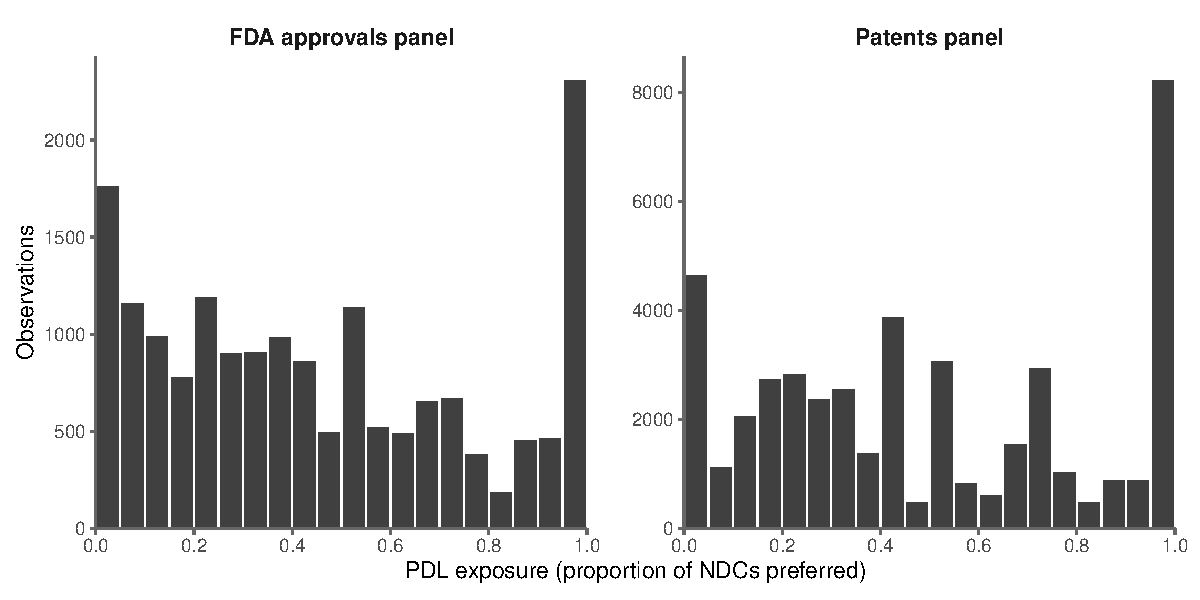
\includegraphics[width=\linewidth]{../output/summary_statistics/pdl_exposure_histogram.pdf}
  \caption{Distribution of PDL exposure in constructed panels}
  \label{fig:pdl_histogram}
\end{figure}

\clearpage

% --- From empirical_results.tex ---

\renewenvironment{table}[1][]{}{}

\subsection{Regression Tables}

\subsubsection{RQ1: Overall Innovation Response}

%TC:ignore
\footnotesize
\input{../output/RQ1/feols_exante_models.tex}
\captionof{table}{FEOLS event-study estimates: overall innovation response (ex-ante)}
\label{tab:rq1_feols_exante}
\normalsize
%TC:endignore

\clearpage

\subsubsection{RQ2: Medicaid Demand and PDL Exposure}

%TC:ignore
\footnotesize
\input{../output/RQ2/feols_exante_models.tex}
\captionof{table}{FEOLS event-study estimates: Medicaid demand and PDL exposure (ex-ante)}
\label{tab:rq2_feols_exante}
\normalsize
%TC:endignore

\clearpage

\subsection{Therapeutic-Class Substitutability}

%TC:ignore
\makeatletter
\renewenvironment{table}[1][H]{\@float{table}[H]}{\end@float}
\makeatother
\input{../output/rebate_exploration/class_substitutability.tex}
\renewenvironment{table}[1][]{}{}
%TC:endignore

\clearpage

% --- From robustness.tex ---

\subsection{Robustness Regression Tables}

\subsubsection{RQ1: Ex-Post FEOLS}

%TC:ignore
\footnotesize
\input{../output/RQ1/feols_expost_models.tex}
\captionof{table}{FEOLS event-study estimates: overall innovation response (ex-post)}
\label{tab:rob_rq1_feols_expost}
\normalsize
%TC:endignore

\begin{figure}[!h]
  \centering
  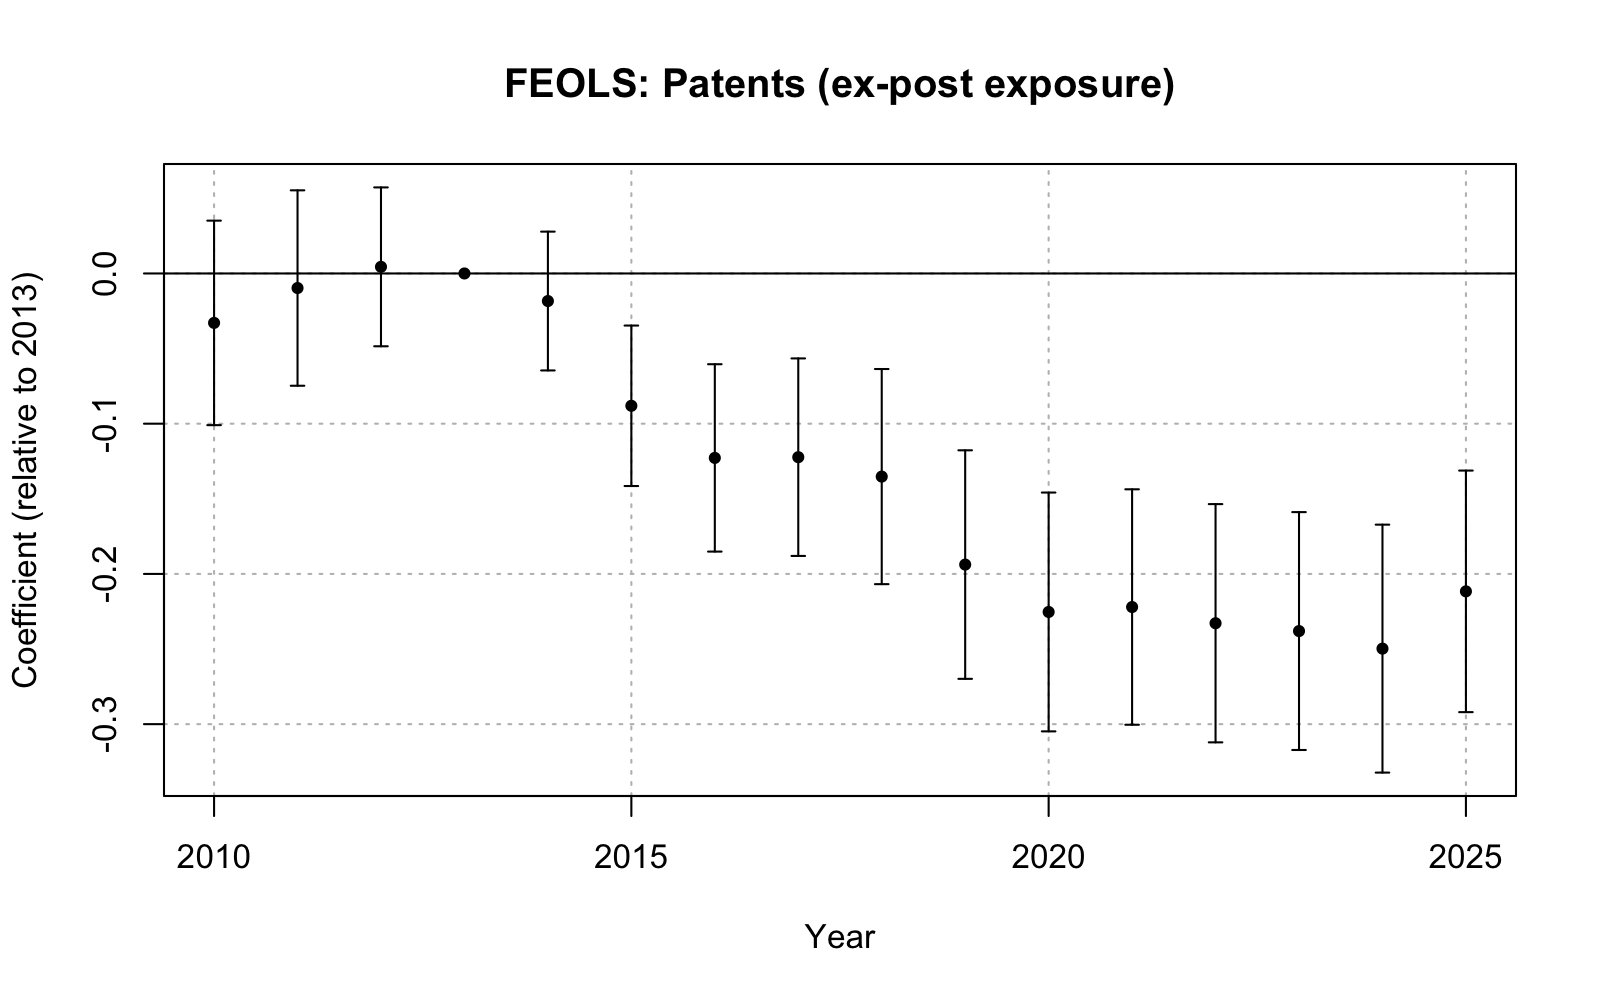
\includegraphics[width=\linewidth]{../output/RQ1/patent_feols_expost.png}
  \caption{FEOLS event study: patents, ex-post Medicaid exposure}
  \label{fig:rob_rq1_patent_feols_expost}
\end{figure}

\begin{figure}[!h]
  \centering
  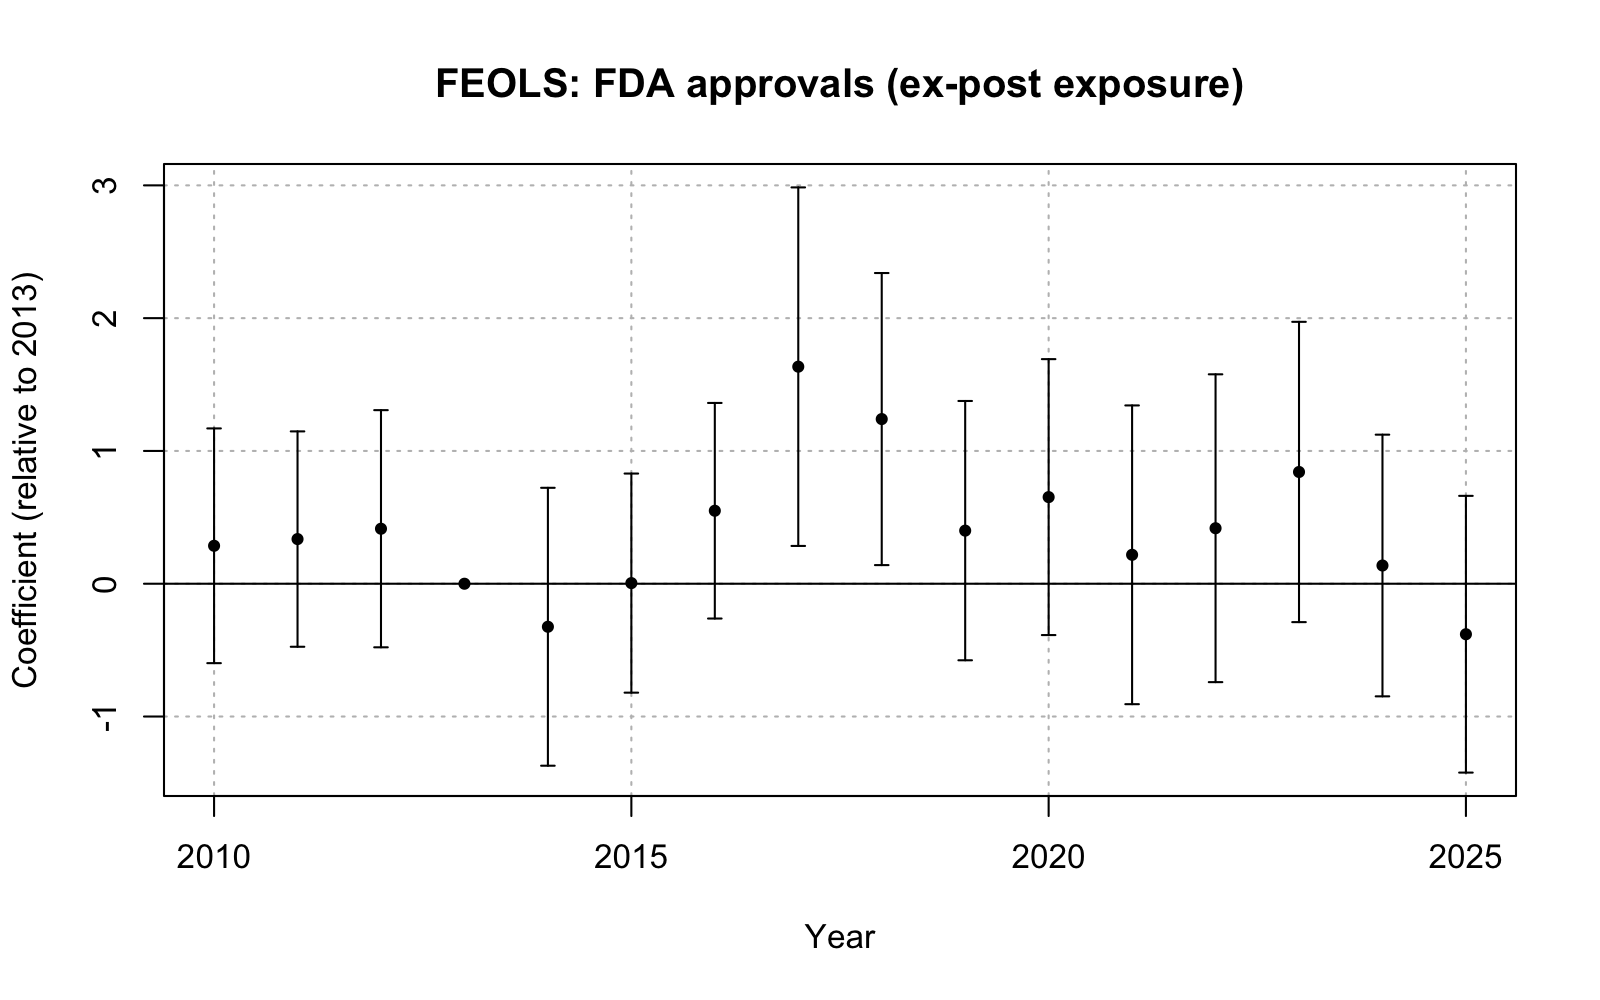
\includegraphics[width=\linewidth]{../output/RQ1/fda_feols_expost.png}
  \caption{FEOLS event study: FDA approvals, ex-post Medicaid exposure}
  \label{fig:rob_rq1_fda_feols_expost}
\end{figure}

\clearpage

\subsubsection{RQ1: Ex-Ante FE Poisson}

%TC:ignore
\footnotesize
\input{../output/RQ1/fepois_exante_models.tex}
\captionof{table}{FE Poisson event-study estimates: overall innovation response (ex-ante)}
\label{tab:rob_rq1_fepois_exante}
\normalsize
%TC:endignore

\begin{figure}[!h]
  \centering
  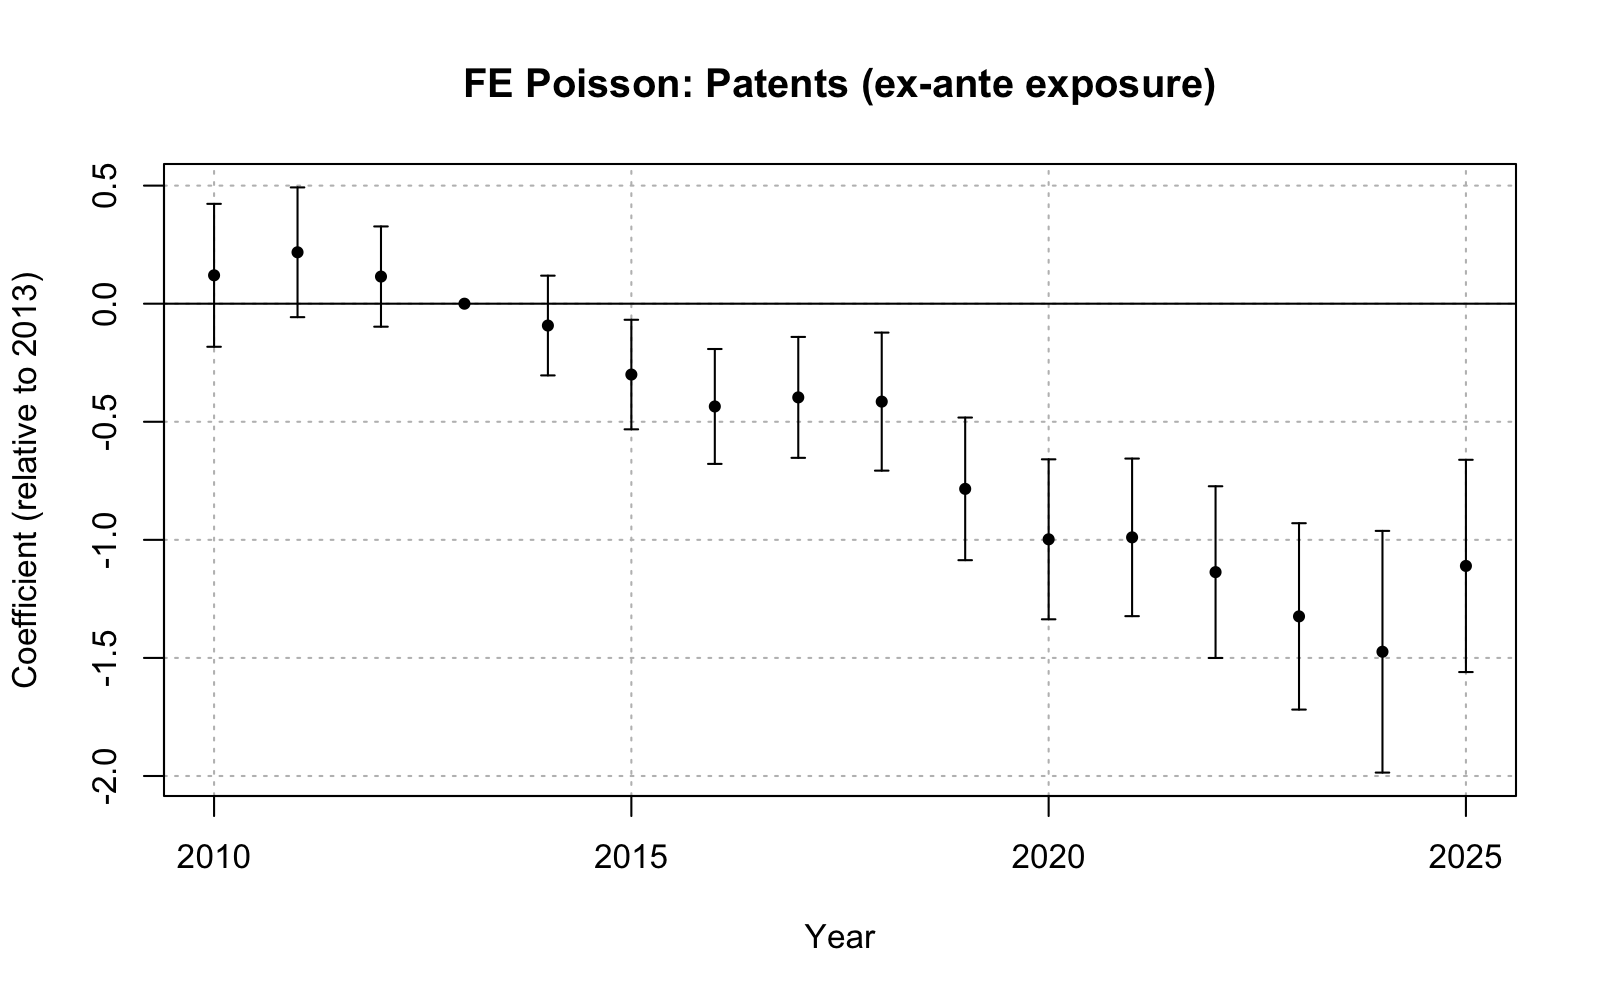
\includegraphics[width=\linewidth]{../output/RQ1/patent_poi_exante.png}
  \caption{FE Poisson event study: patents, ex-ante Medicaid exposure}
  \label{fig:rob_rq1_patent_poi_exante}
\end{figure}

\begin{figure}[!h]
  \centering
  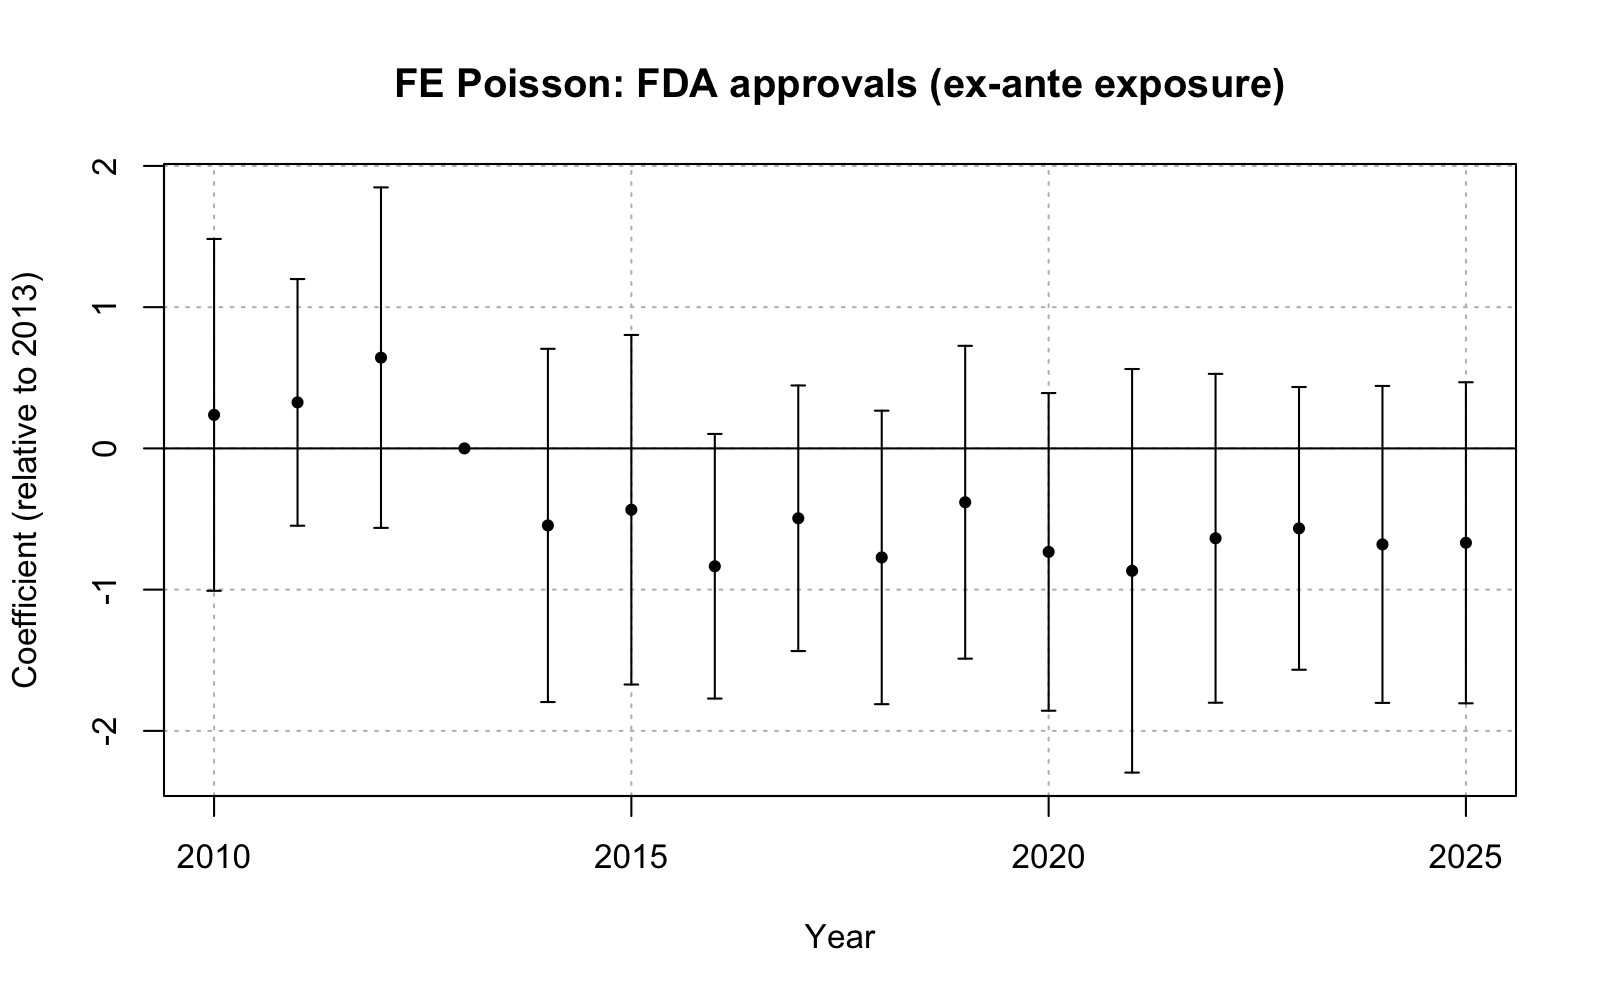
\includegraphics[width=\linewidth]{../output/RQ1/fda_poi_exante.png}
  \caption{FE Poisson event study: FDA approvals, ex-ante Medicaid exposure}
  \label{fig:rob_rq1_fda_poi_exante}
\end{figure}

\clearpage

\subsubsection{RQ1: Ex-Post FE Poisson}

%TC:ignore
\footnotesize
\input{../output/RQ1/fepois_expost_models.tex}
\captionof{table}{FE Poisson event-study estimates: overall innovation response (ex-post)}
\label{tab:rob_rq1_fepois_expost}
\normalsize
%TC:endignore

\begin{figure}[!h]
  \centering
  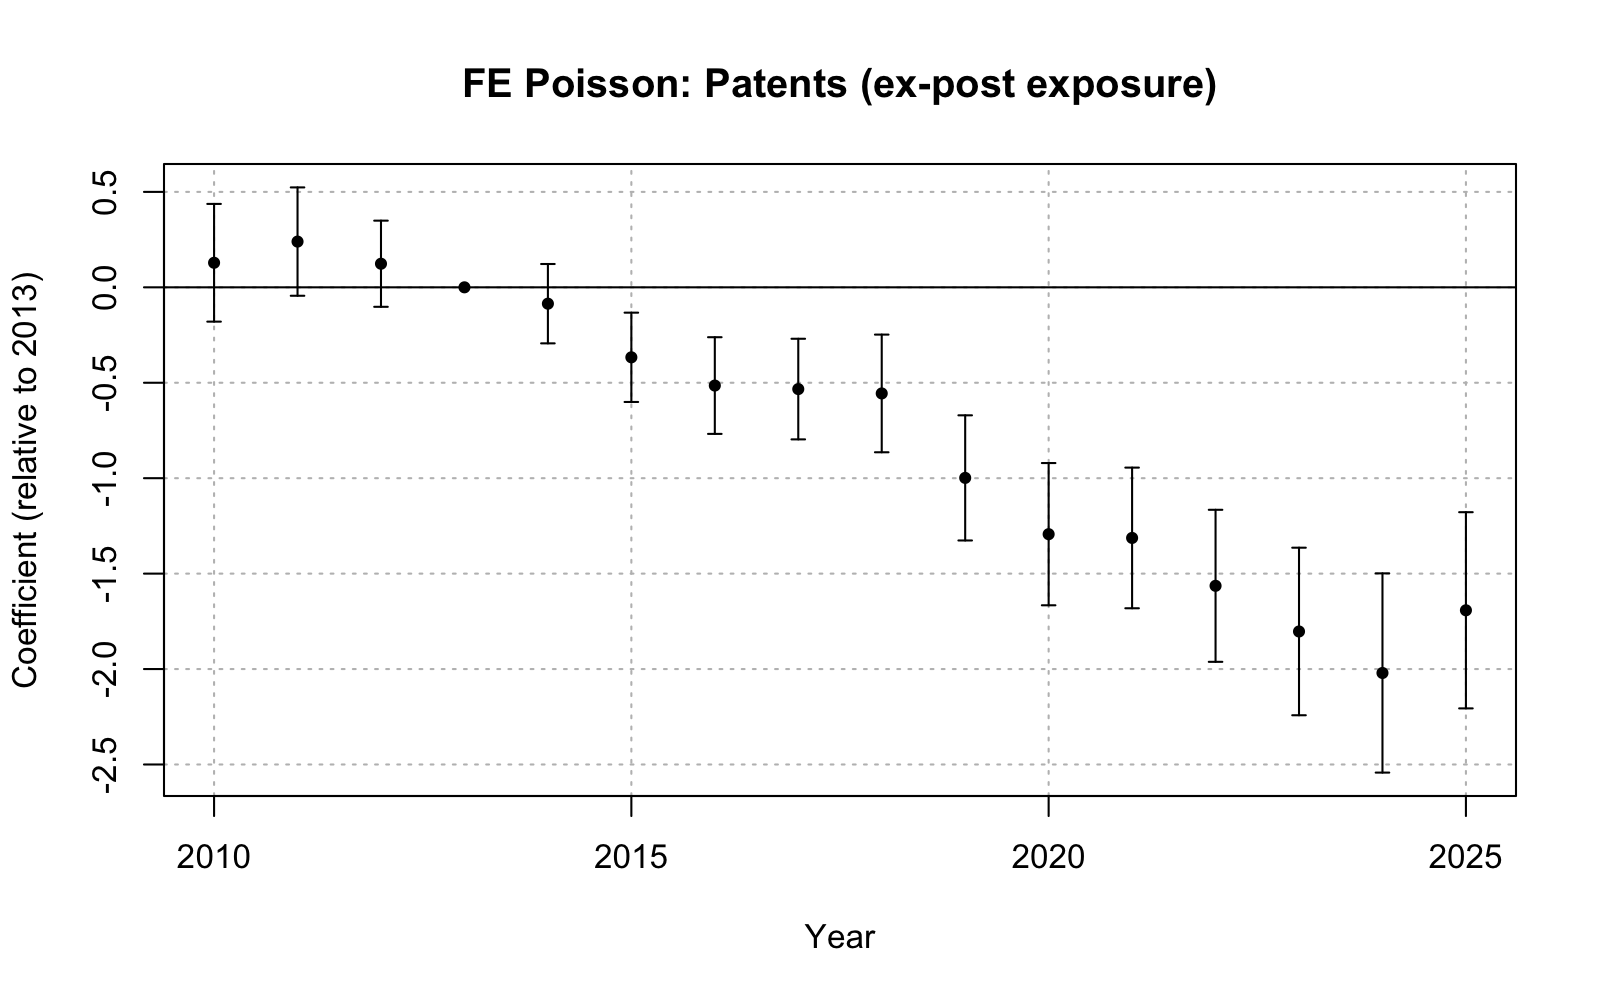
\includegraphics[width=\linewidth]{../output/RQ1/patent_poi_expost.png}
  \caption{FE Poisson event study: patents, ex-post Medicaid exposure}
  \label{fig:rob_rq1_patent_poi_expost}
\end{figure}

\begin{figure}[!h]
  \centering
  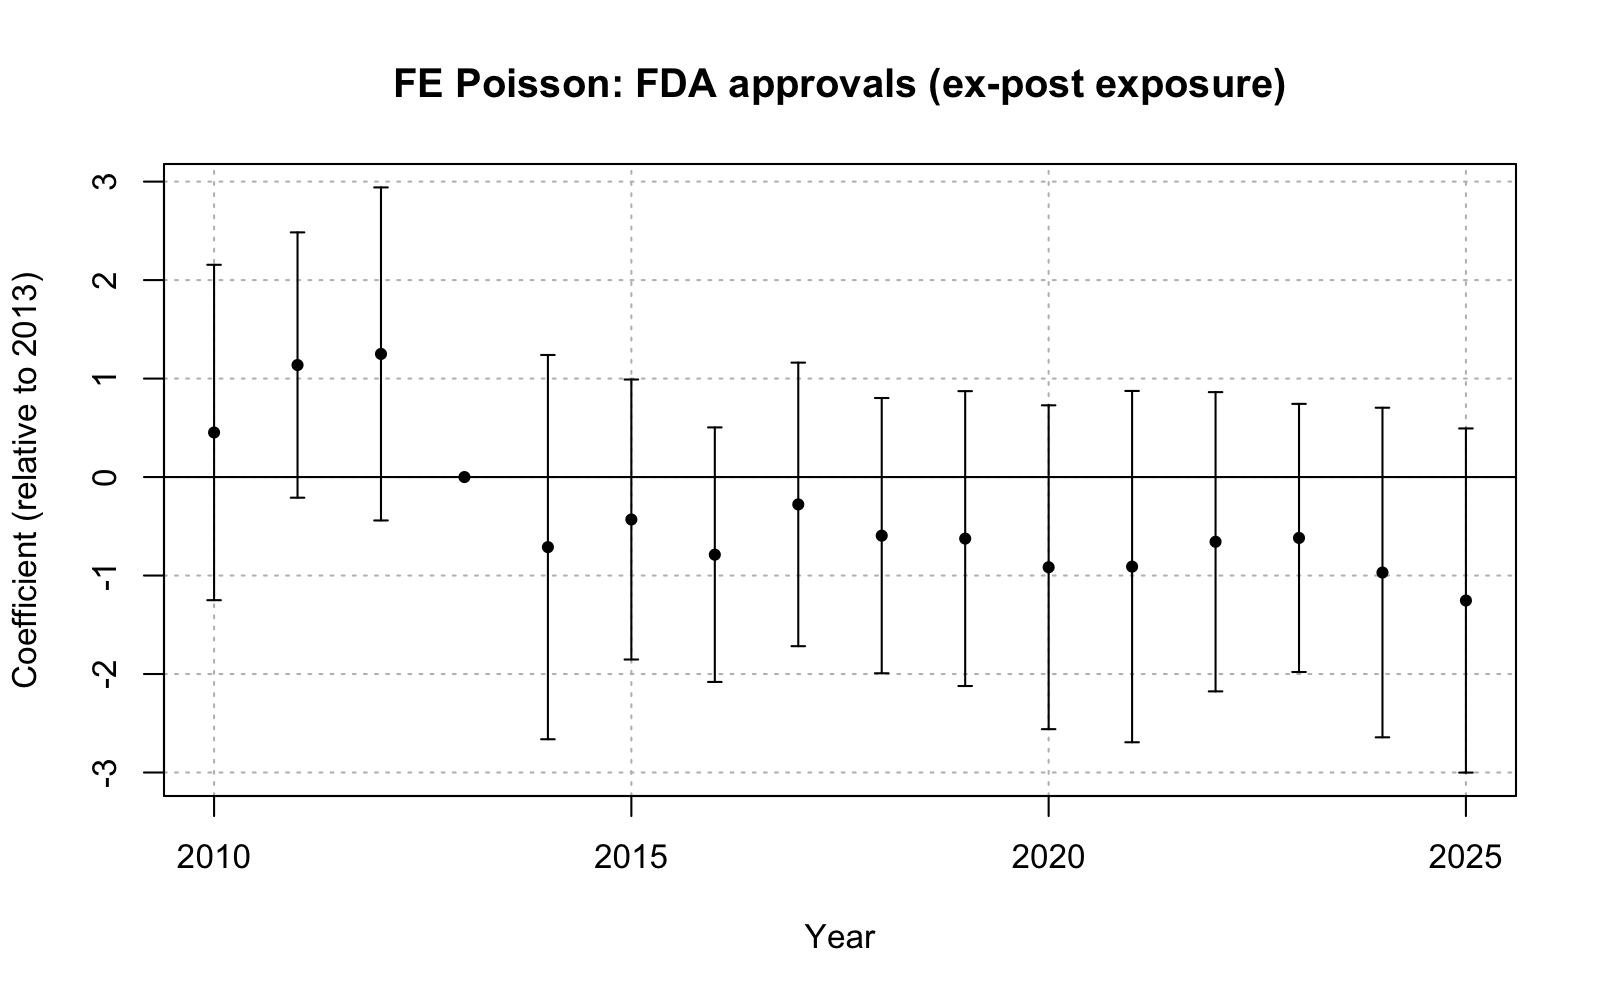
\includegraphics[width=\linewidth]{../output/RQ1/fda_poi_expost.png}
  \caption{FE Poisson event study: FDA approvals, ex-post Medicaid exposure}
  \label{fig:rob_rq1_fda_poi_expost}
\end{figure}

\clearpage

\subsubsection{RQ1: Binned Treatment}

%TC:ignore
\makeatletter
\renewenvironment{table}[1][H]{\@float{table}[H]}{\end@float}
\makeatother
\input{../output/robustness/binned_treatment/atc_bins.tex}
\renewenvironment{table}[1][]{}{}
%TC:endignore

%TC:ignore
\footnotesize
\input{../output/robustness/binned_treatment/binned_models.tex}
\captionof{table}{Binned treatment event-study estimates (FEOLS, ex-ante)}
\label{tab:rob_binned}
\normalsize
%TC:endignore

\begin{figure}[!h]
  \centering
  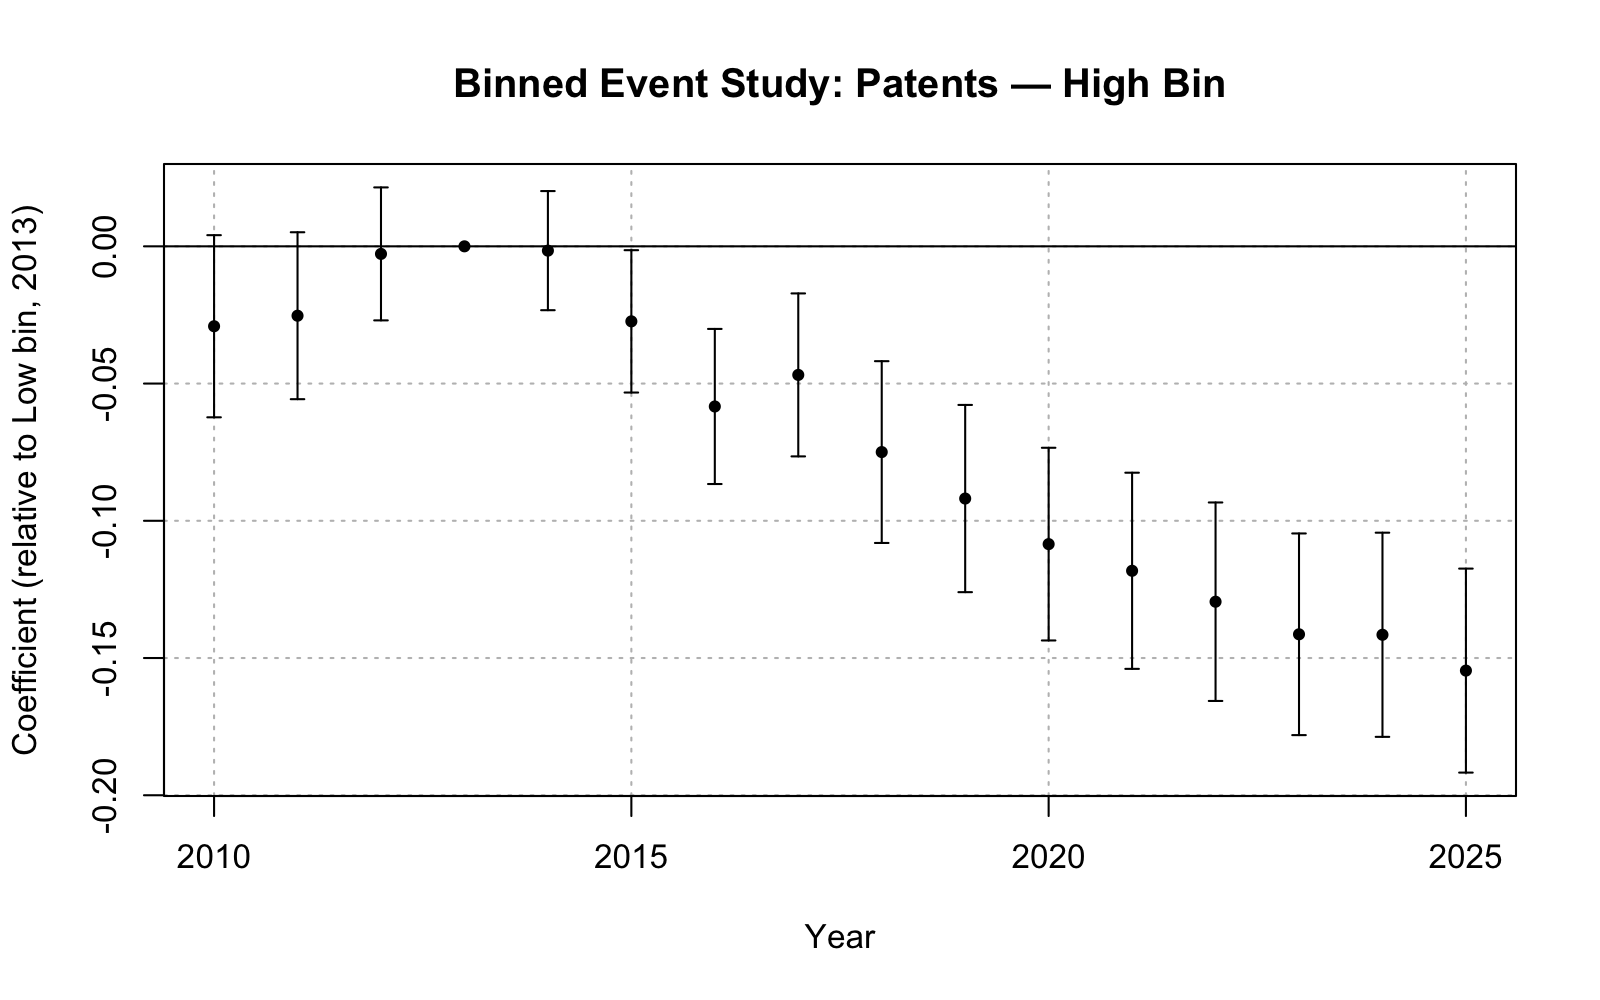
\includegraphics[width=\linewidth]{../output/robustness/binned_treatment/binned_patent_high_es.png}
  \caption{Binned event study: patents, high-exposure bin (N, C)}
  \label{fig:rob_binned_patent_high}
\end{figure}

\begin{figure}[!h]
  \centering
  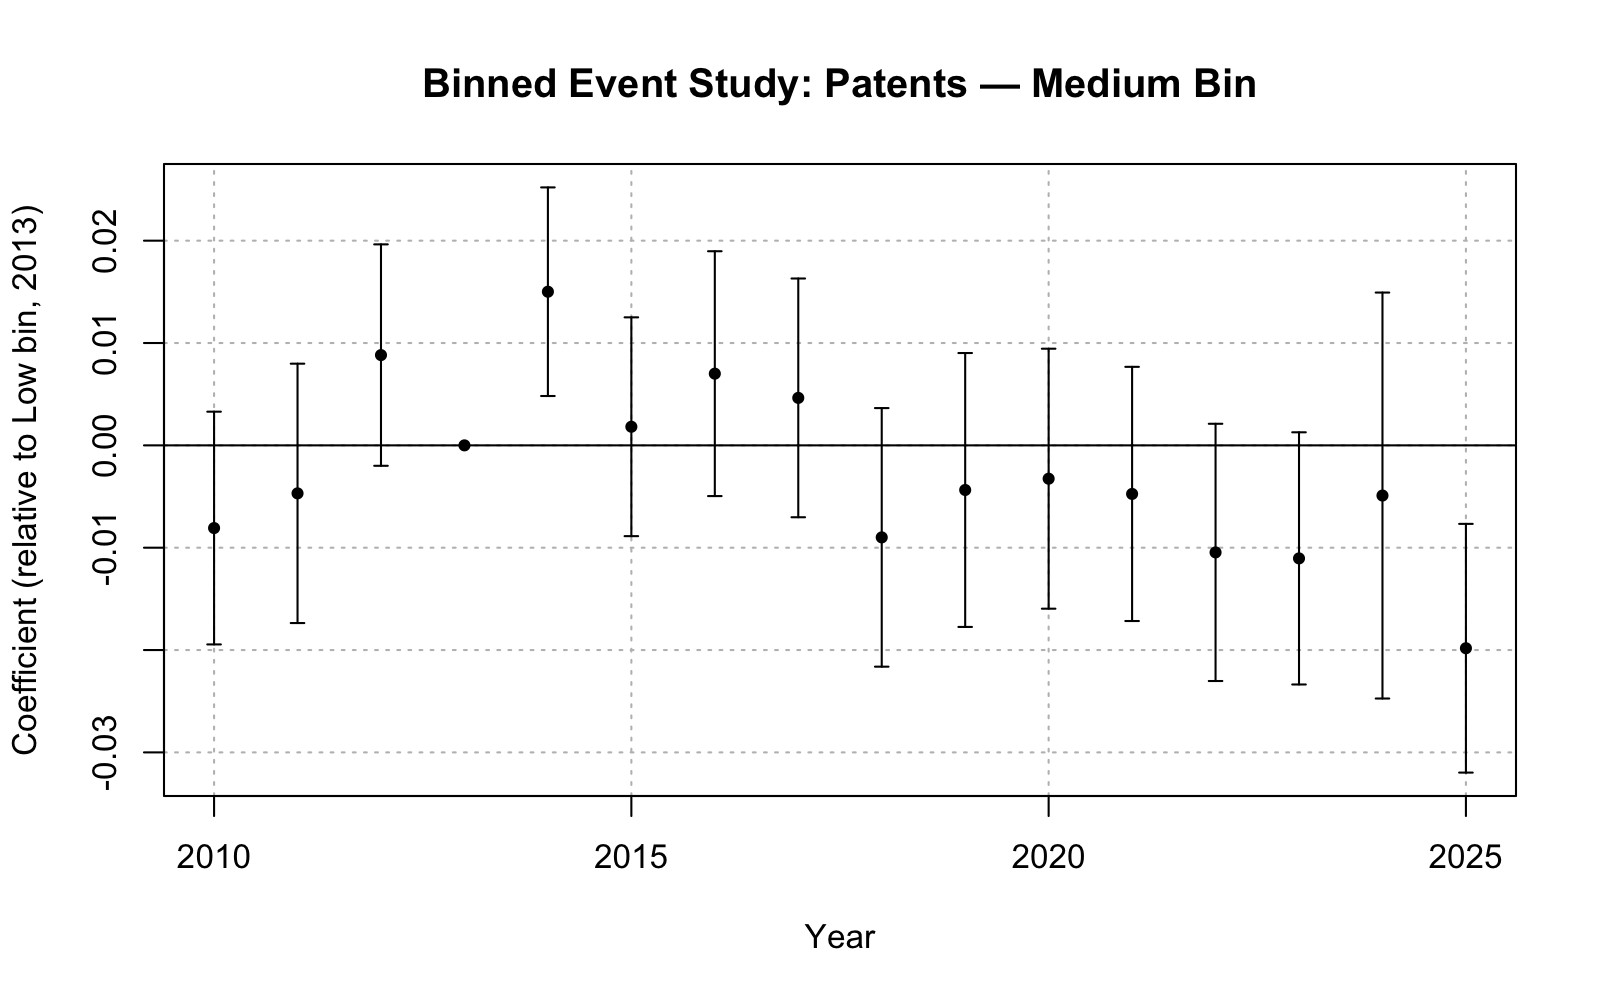
\includegraphics[width=\linewidth]{../output/robustness/binned_treatment/binned_patent_medium_es.png}
  \caption{Binned event study: patents, medium-exposure bin (J, D)}
  \label{fig:rob_binned_patent_medium}
\end{figure}

\clearpage

\begin{figure}[!h]
  \centering
  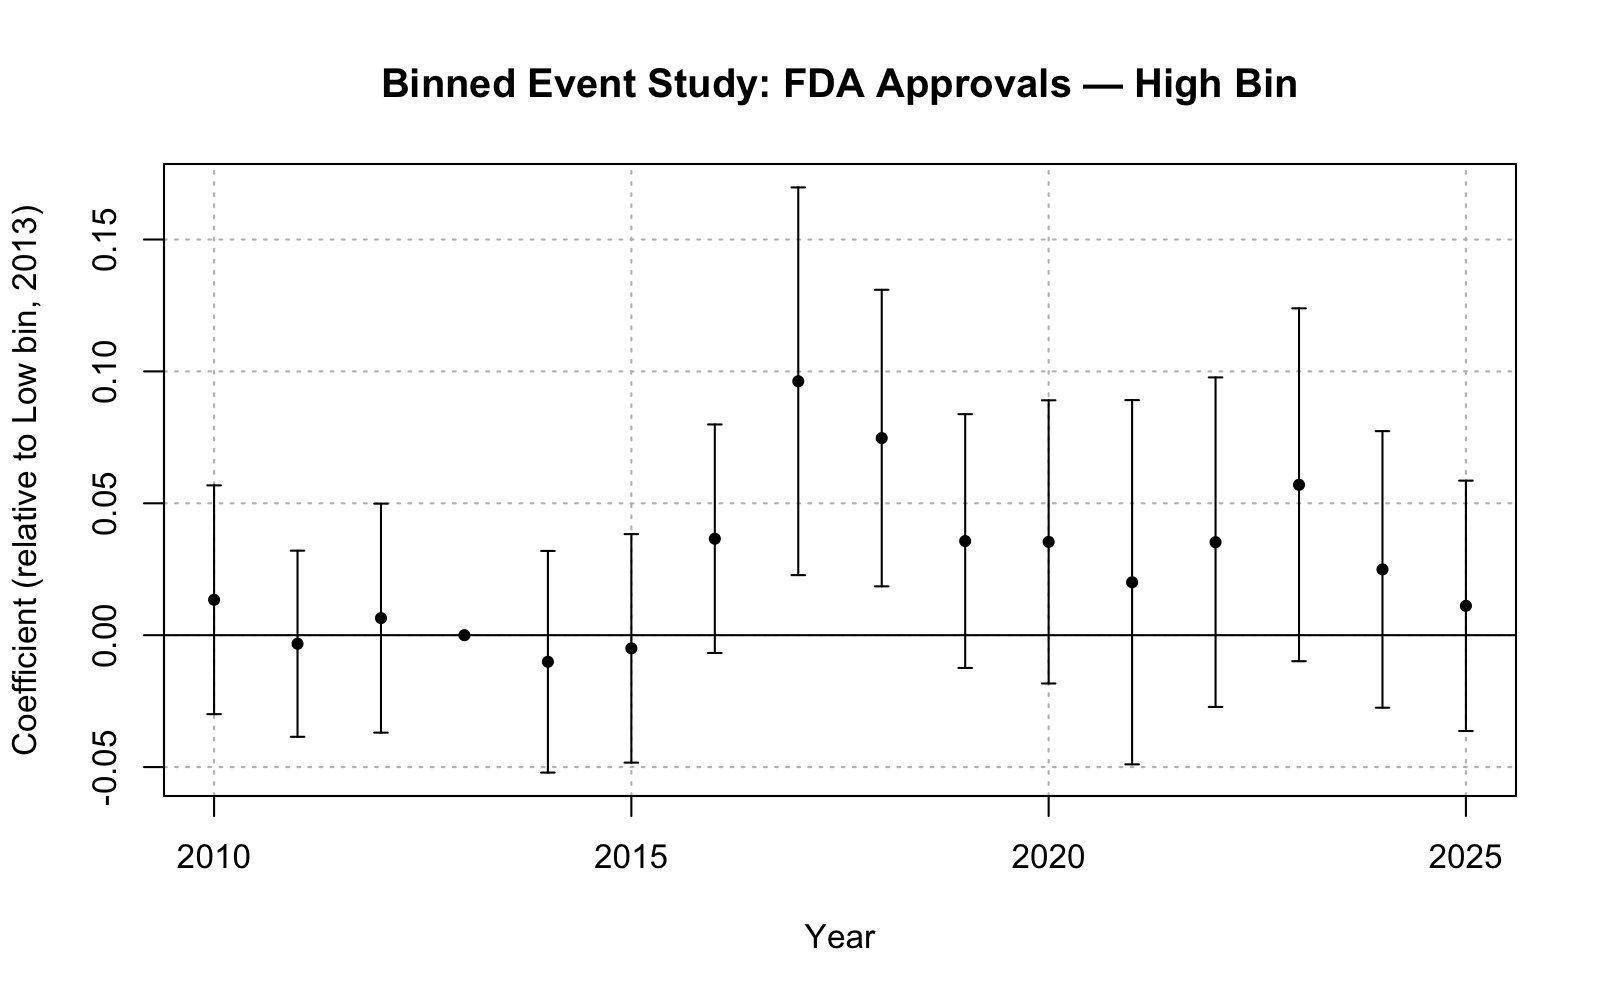
\includegraphics[width=\linewidth]{../output/robustness/binned_treatment/binned_fda_high_es.png}
  \caption{Binned event study: FDA approvals, high-exposure bin (N, C)}
  \label{fig:rob_binned_fda_high}
\end{figure}

\begin{figure}[!h]
  \centering
  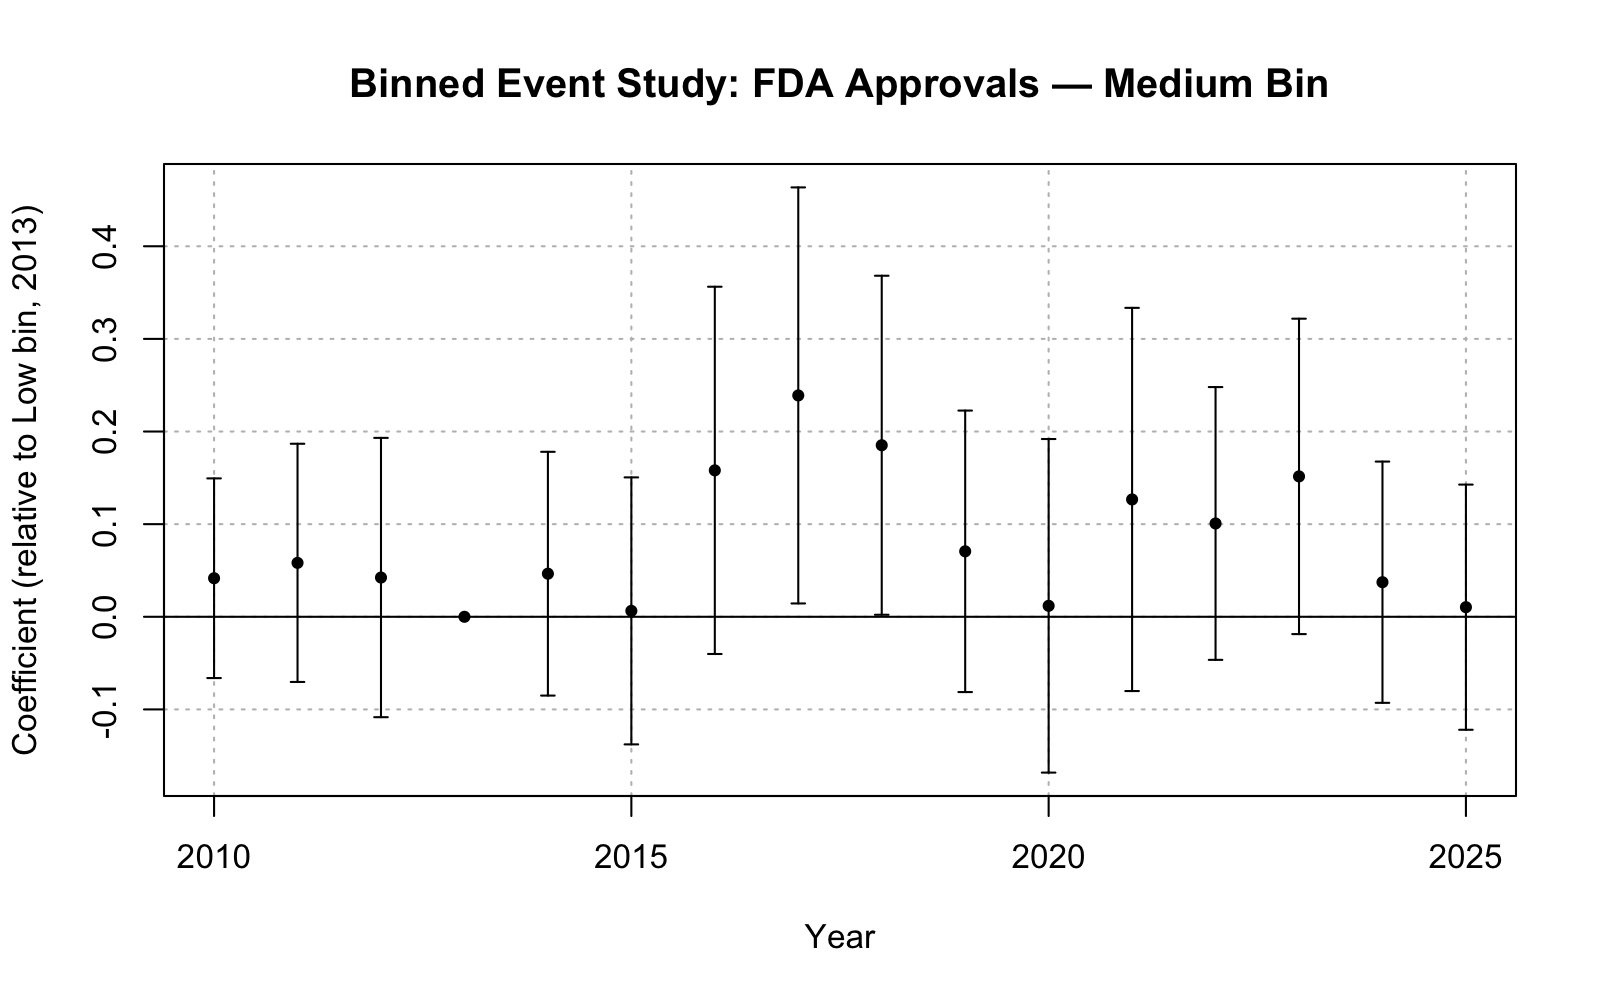
\includegraphics[width=\linewidth]{../output/robustness/binned_treatment/binned_fda_medium_es.png}
  \caption{Binned event study: FDA approvals, medium-exposure bin (J, D)}
  \label{fig:rob_binned_fda_medium}
\end{figure}

\clearpage

\subsubsection{RQ1: Continuous Difference-in-Differences}

%TC:ignore
\makeatletter
\renewenvironment{table}[1][H]{\@float{table}[H]}{\end@float}
\makeatother
\footnotesize
\input{../output/robustness/contdid/contdid_es.tex}
\normalsize
\renewenvironment{table}[1][]{}{}
%TC:endignore

\begin{figure}[!h]
  \centering
  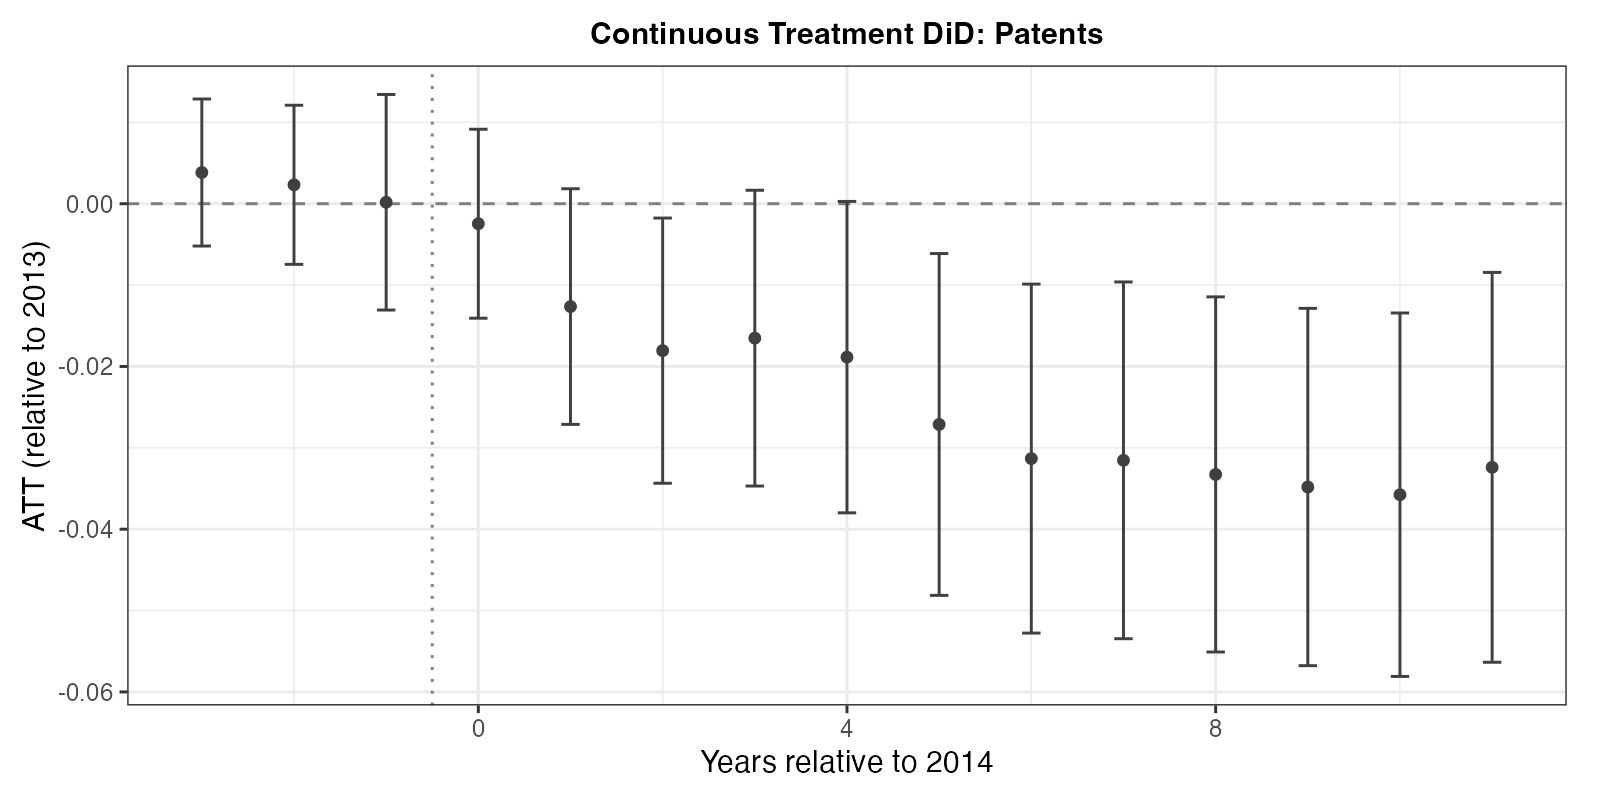
\includegraphics[width=\linewidth]{../output/robustness/contdid/contdid_patent_es.png}
  \caption{Continuous DiD event study: patents}
  \label{fig:rob_contdid_patent}
\end{figure}

\begin{figure}[!h]
  \centering
  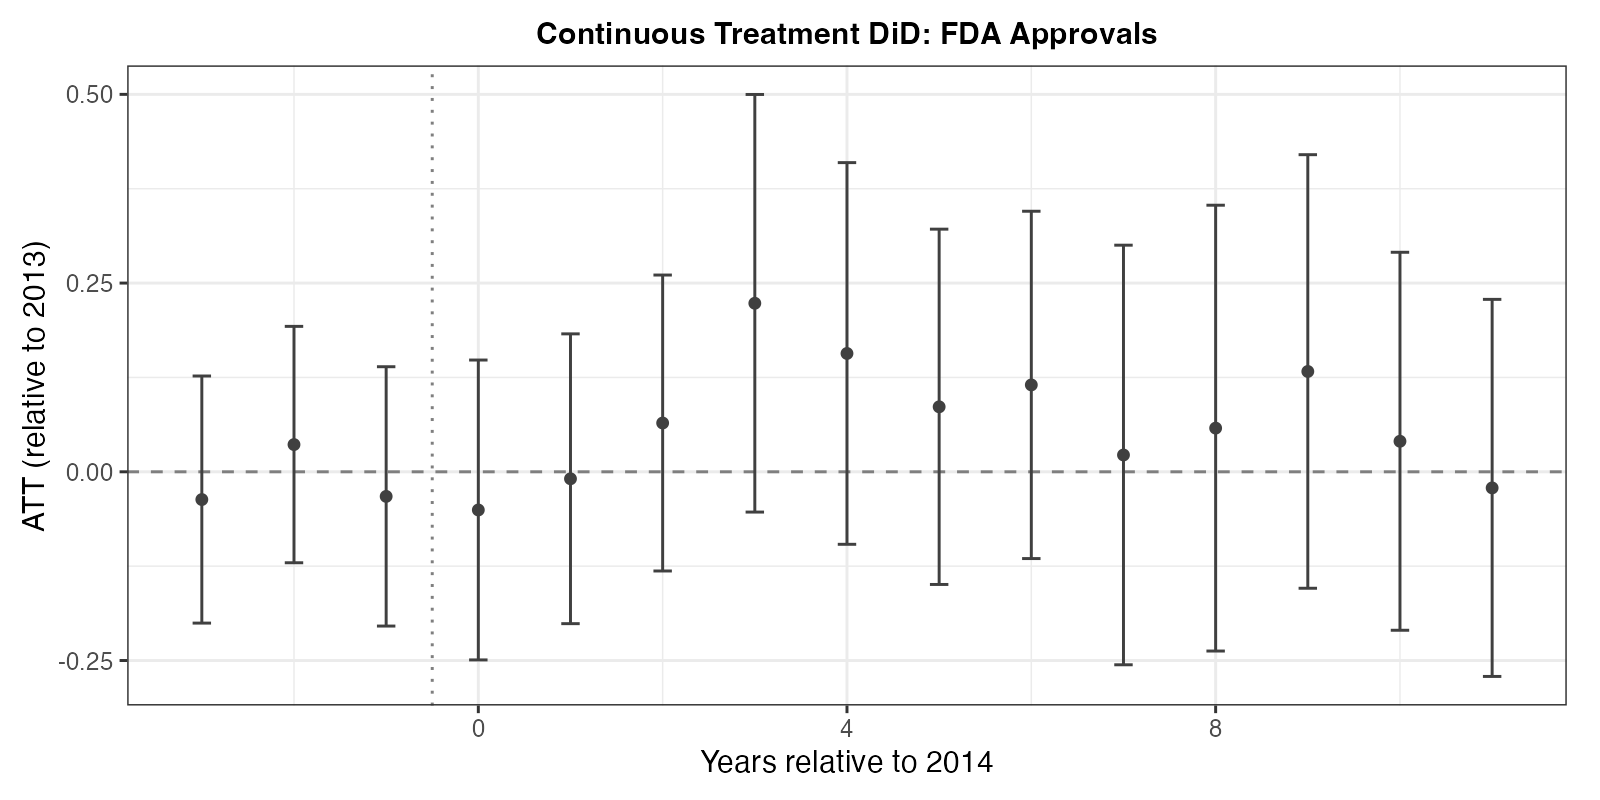
\includegraphics[width=\linewidth]{../output/robustness/contdid/contdid_fda_es.png}
  \caption{Continuous DiD event study: FDA approvals}
  \label{fig:rob_contdid_fda}
\end{figure}

\clearpage

\subsubsection{RQ2: Ex-Post FEOLS}

%TC:ignore
\footnotesize
\input{../output/RQ2/feols_expost_models.tex}
\captionof{table}{FEOLS event-study estimates: Medicaid demand and PDL exposure (ex-post)}
\label{tab:rob_rq2_feols_expost}
\normalsize
%TC:endignore

\begin{figure}[!h]
  \centering
  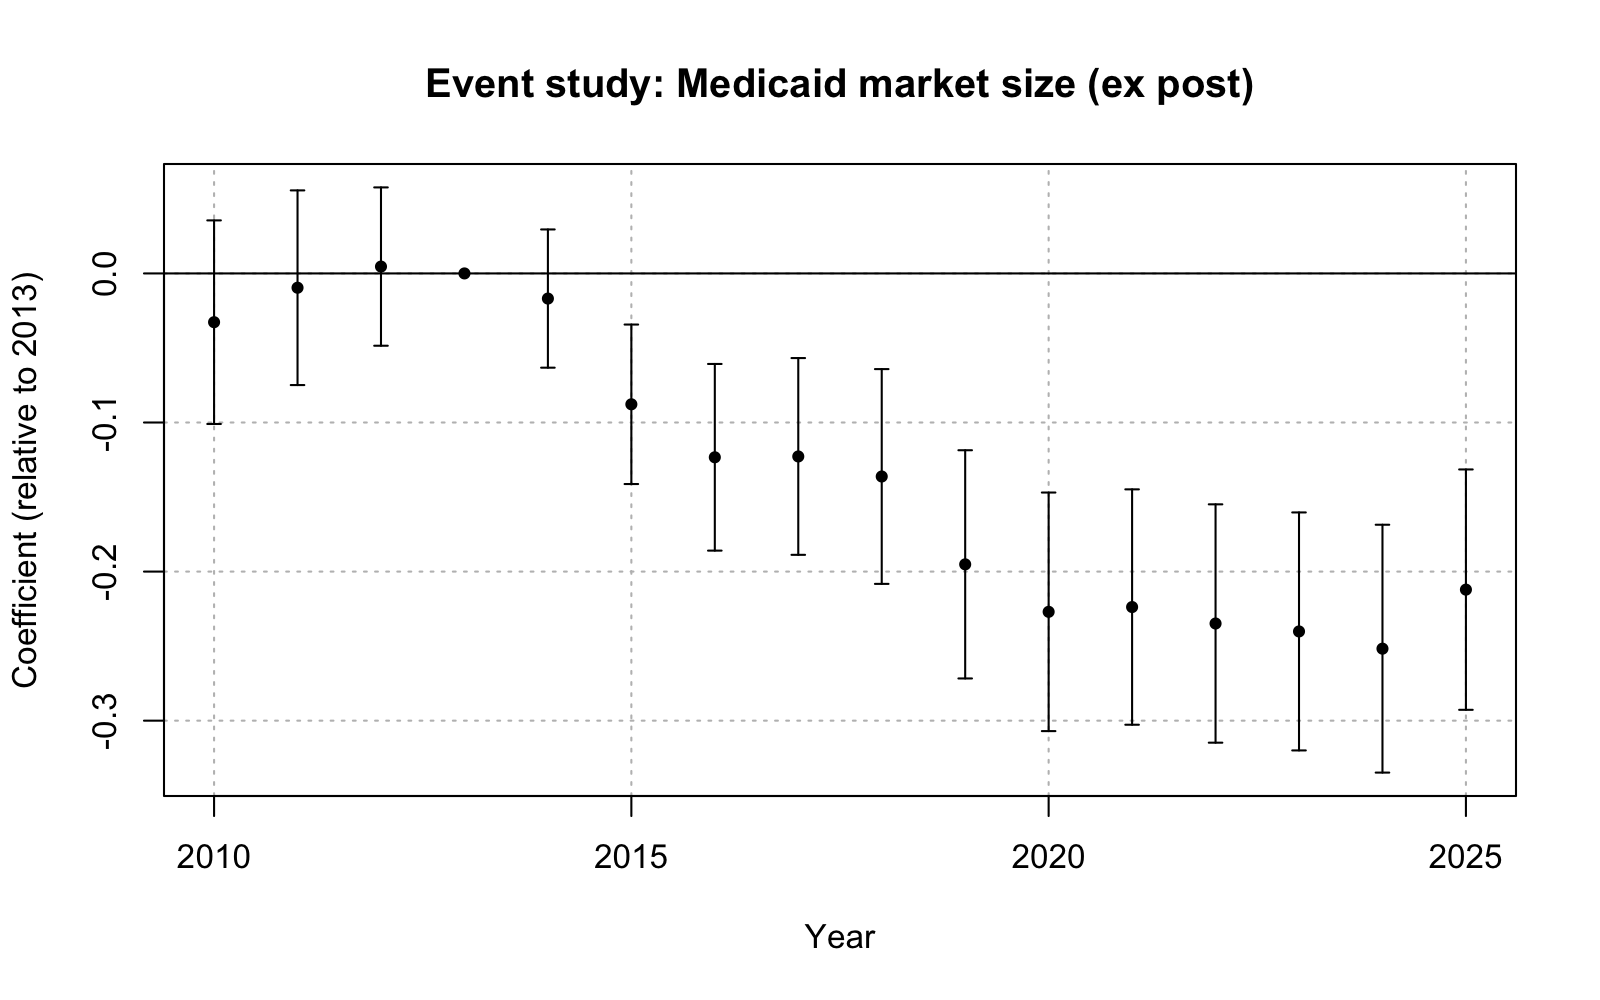
\includegraphics[width=\linewidth]{../output/RQ2/patent_feols_expost_medicaid.png}
  \caption{FEOLS event study: patents, Medicaid exposure (ex-post)}
  \label{fig:rob_rq2_patent_expost_medicaid}
\end{figure}

\begin{figure}[!h]
  \centering
  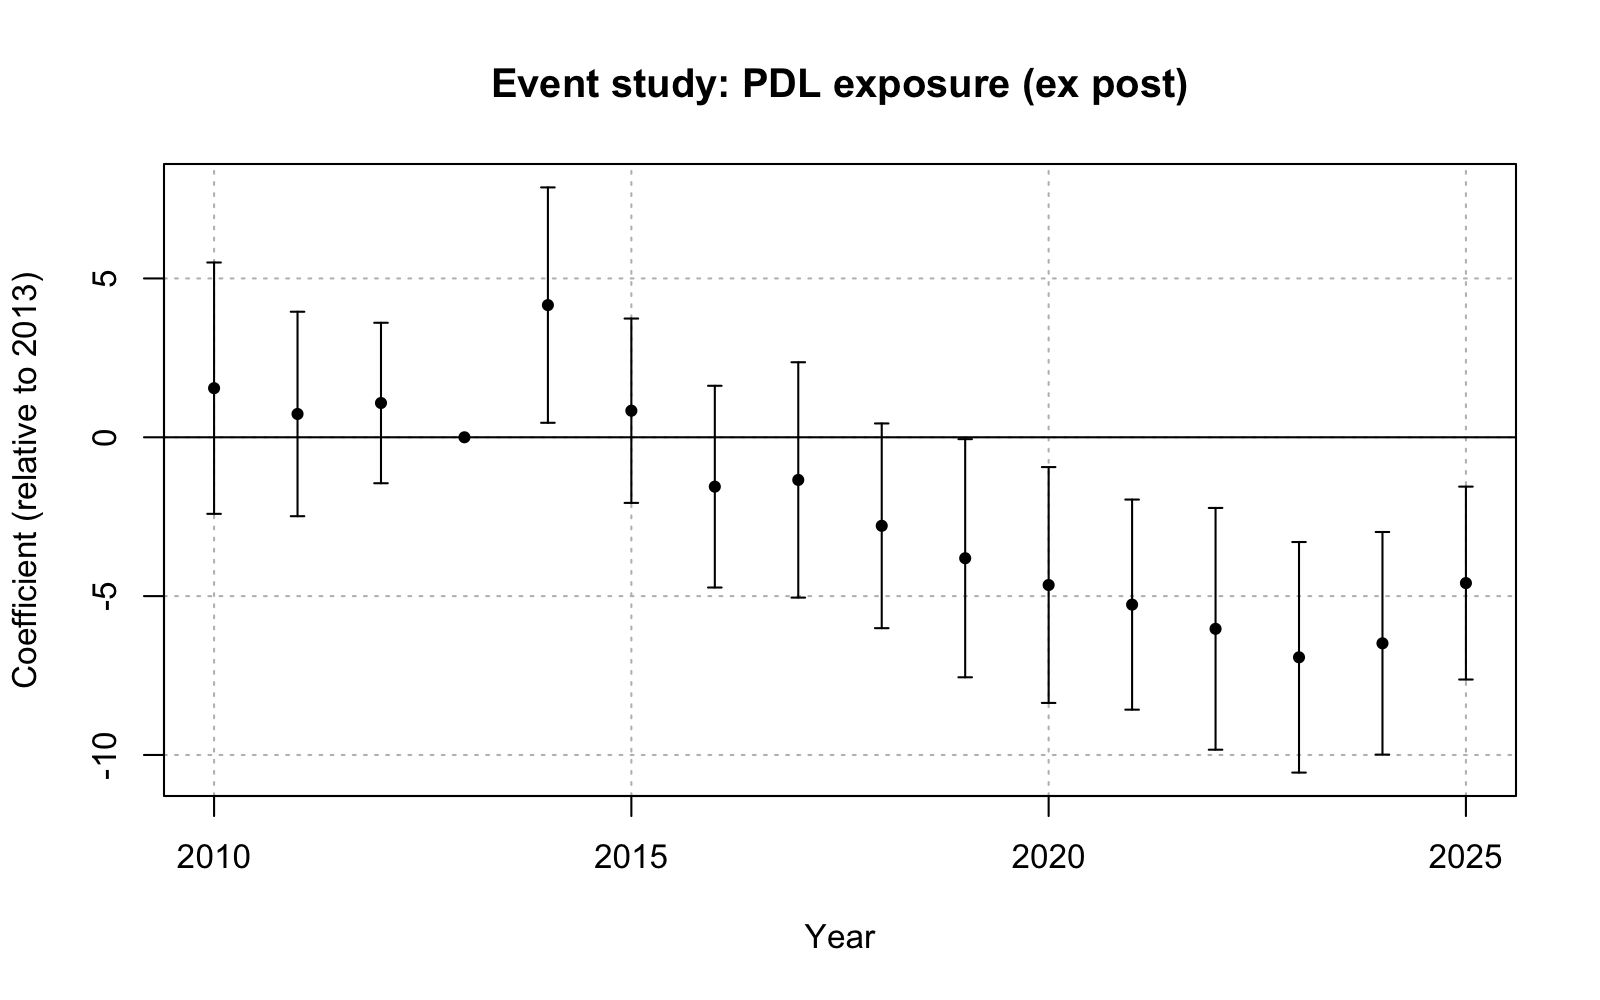
\includegraphics[width=\linewidth]{../output/RQ2/patent_feols_expost_pdl.png}
  \caption{FEOLS event study: patents, PDL exposure (ex-post)}
  \label{fig:rob_rq2_patent_expost_pdl}
\end{figure}

\clearpage

\begin{figure}[!h]
  \centering
  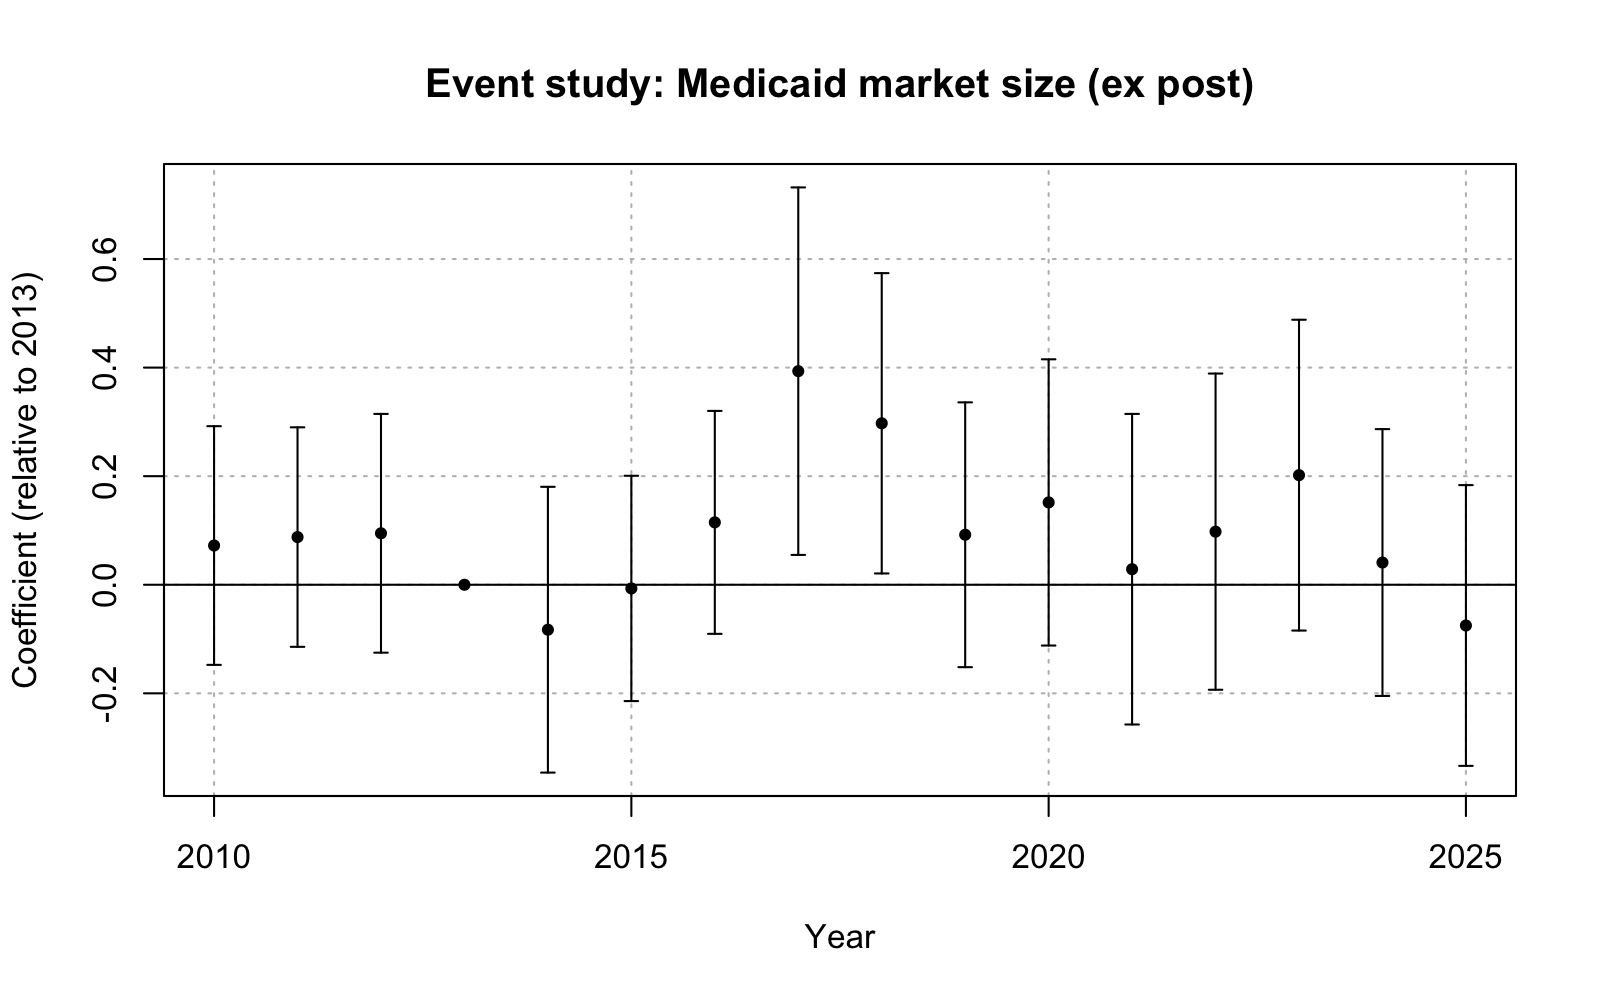
\includegraphics[width=\linewidth]{../output/RQ2/fda_feols_expost_medicaid.png}
  \caption{FEOLS event study: FDA approvals, Medicaid exposure (ex-post)}
  \label{fig:rob_rq2_fda_expost_medicaid}
\end{figure}

\begin{figure}[!h]
  \centering
  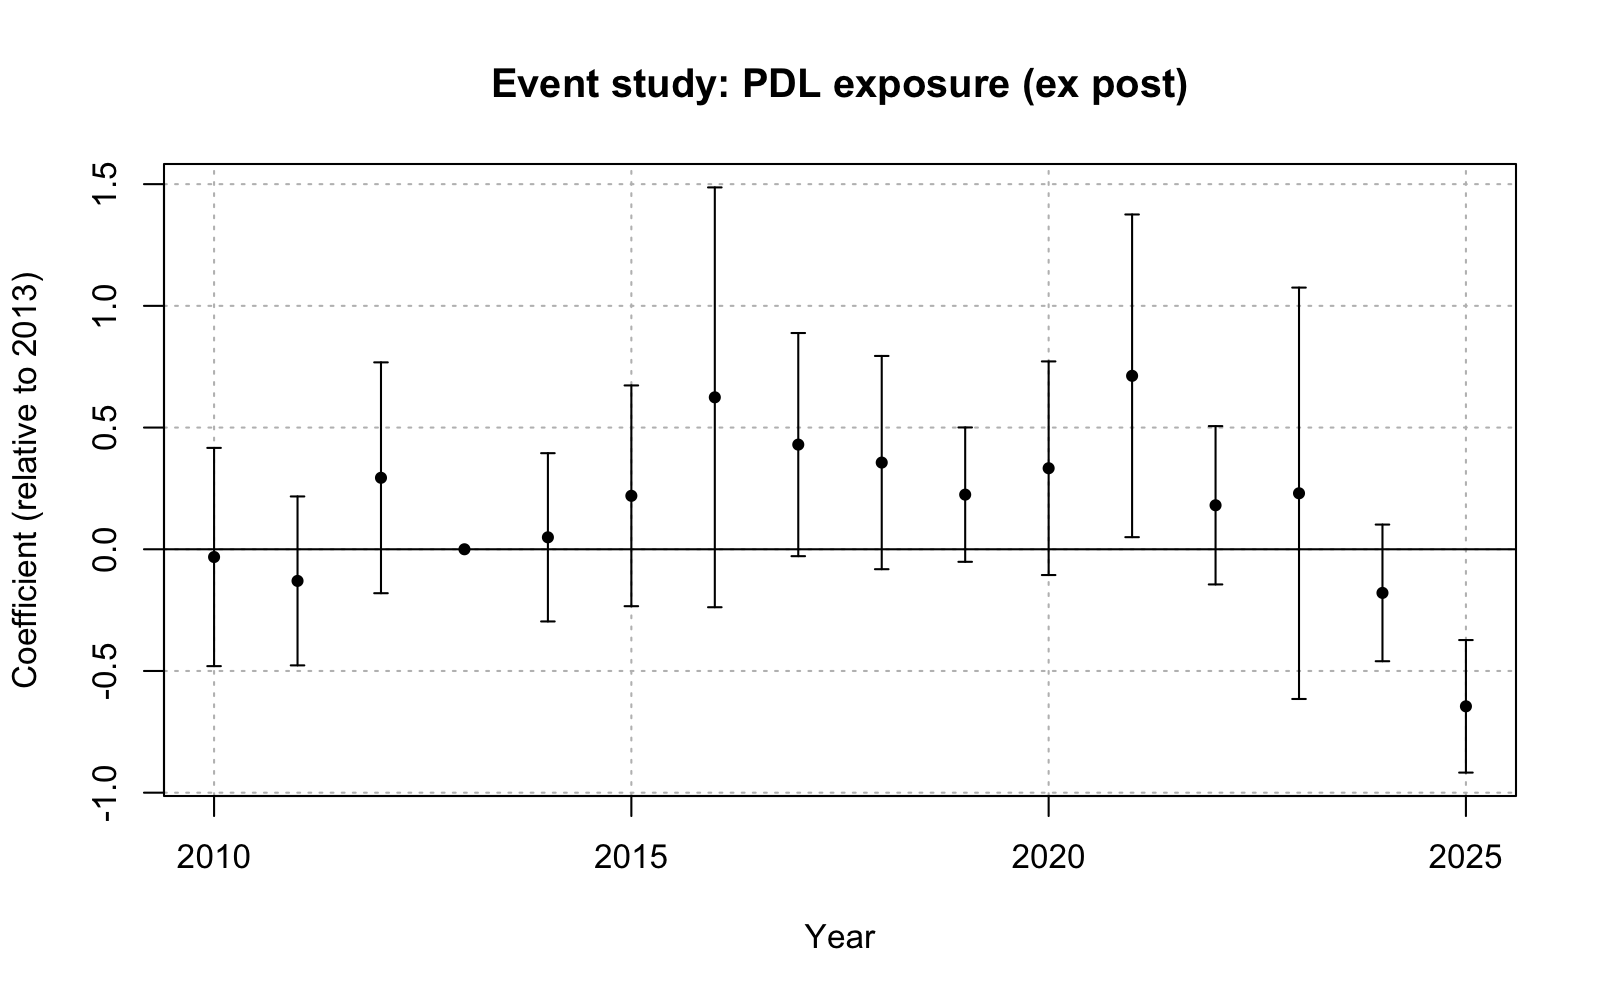
\includegraphics[width=\linewidth]{../output/RQ2/fda_feols_expost_pdl.png}
  \caption{FEOLS event study: FDA approvals, PDL exposure (ex-post)}
  \label{fig:rob_rq2_fda_expost_pdl}
\end{figure}

\clearpage

\subsubsection{RQ3: Ex-Post FEOLS}

%TC:ignore
\footnotesize
\input{../output/RQ3/feols_expost_models.tex}
\captionof{table}{Triple-difference estimates: therapeutic-class heterogeneity (FEOLS, ex-post)}
\label{tab:rob_rq3_feols_expost}
\normalsize
%TC:endignore

\clearpage

% --- From theoretical_model.tex ---

\subsection{Baseline Model Parameters} \label{app:parameters}

Table~\ref{tab:parameters} reports the baseline parameter values used to generate Figure~\ref{fig:comp_statics}. Parameters that are not varied are held at these baseline values.

%TC:ignore
\makeatletter
\renewenvironment{table}[1][H]{\@float{table}[H]}{\end@float}
\makeatother
\input{../output/theoretical_model/parameters.tex}
\renewenvironment{table}[1][]{}{}
%TC:endignore

\end{document}
%
}

\begin{document}

% ===== Title Page =====
\begin{titlepage}
  \centering
  \vspace*{3cm}
  {\LARGE\bfseries MPhil Thesis\par}
  \vspace{1.5cm}
  {\Large Mohammad-Shah Karim\par}
  \vspace{1cm}
  {\large May 2026\par}
  \vspace{2cm}
  {\large Word count: \totalwordcount\par}
  \vfill
\end{titlepage}

% ===== Table of Contents =====
\mastertoc
\newpage

% ===== Main Body =====
\documentclass[12pt]{article}
\usepackage{geometry}
\geometry{a4paper, portrait, margin=1in}

% --- Math Packages ---
\usepackage{amsmath}
\usepackage{amssymb}
\usepackage{amsfonts}
\usepackage{amsthm}

% --- Graphics & Diagrams ---
\usepackage{graphicx}
\usepackage{tikz}
\usetikzlibrary{shapes, arrows, positioning}

% --- Formatting ---
\usepackage{parskip}
\usepackage[hidelinks]{hyperref}
\usepackage{natbib}
\usepackage{enumitem}
\pagestyle{plain}

\title{MPhil Thesis: Introduction}
\author{Mohammad-Shah Karim}
\date{April 2026}

\begin{document}

\maketitle

\section{Introduction}

Pharmaceutical innovation is central towards long-run improvements in health and welfare. New drugs can improve quantity of life while changing the treatment possibilities which are available for physicians to administer on patients. At the same time, pharmaceutical innovation is unusually sensitive to policy. Development of a new drug requires a large upfront investment with a long development horizon including patent applications and clinical trials, with only a high probability of failure. Since the returns to a successful drug accrue over multiple years and depend on both prices and the volumes that prevail within the market, the incentives to undertake the investment to develop a drug are shaped not only by opportunity, but also by the economic and institutional environment present which determine the expected future profits once the drug reaches the market.

This makes the pharmaceutical market within the United States of America an ideal setting for studying how public policy shapes scientific opportunity. Federal and state governments are now responsible for roughly half of all prescription drug spending (INSERT SOURCE HERE), both as direct purchasers through programmes such as Medicaid and Medicare, and also indirectly through the tax preferences and regulatory rules that govern private insurance. Medicaid is especially important in this respect - it is a large public buyer, but it does not operate as a standard private insurer. Manufacturers that wish to have Medicaid coverage must participate in the Medicaid Drug rebate Program, and states can use Preferred Drug Lists (PDLs) in order to negotiate additional rebates in exchange for preferred formulary placement. Given this, Medicaid demand passes through a public procurement system with statutory and supplement rebates in addition to state level formulary bargaining, thus it cannot be treated as additional market demand.

This thesis examines the consequences of one of such reforms for pharmaceutical innovation - the 2014 Medicaid expansion under the the Patient Protection and Affordable Care Act (ACA). The reform produced a well-documented expansion in the size of the Medicaid market, with population coverage increasing by close to twenty million enrollees int he years following the policy change (INSERT SOURCE HERE). Under standard market-sized frameworks in the pharmaceutical sector this should increase innovation incentives for drug-classes more exposed to Medicaid demand \citep{finkelstein2004static, dubois2015market}. If firms expect to sell more units after a successful round of innovation, the expected returns to R\&D rise. However, the expansion of Medicaid took place inside a procurement framework that combined two features of that are unusual under the standards of a private insurer. A statutory rebate schedule that mechanically transfers a share of any list-price revenue back to the state, and a state-administered formulary system in which Preferred Drug Lists (PDLs) determine which products are reimbursed without prior authorisation. Thus the institutional features meant that an expansion of Medicaid was not simply a positive demand shock for pharmaceutical firm.

The Medicaid setting therefore complicates the prediction under standard pharmaceutical market-sized frameworks. The ACA did not only expand the number of beneficiaries under Medicaid, but it also raised the statutory rebate percentages and extended rebate obligations to Medicaid managed care. Therefore, the reform increased the size of the public market while also increasing the share of revenue back to the state. Additionally, as Medicaid demand grows, preferred placement on a state PDL becomes more valuable. States can use this to negotiate deeper rebates from manufacturers. The same policy may therefore generate two opposing effects. On the one hand, Medicaid expansion raises demand. On the other hand, it may increase pricing pressure and reduce the surplus that firms can capture from that demand.

This thesis therefore raises the question of whether the ACA-induced Medicaid expansion raised pharmaceutical innovation, and whether the response dependent on a firm's exposure to the Medicaid procurement institutions. Put simply, was the expected positive relationship between market size and innovation weakened when the additional demand flows through a state-wide monopsony. Many current drug-pricing reforms, including recent Medicare negotiation policies, rely on the same basic trade-off: lowering public spending and consumer prices may increase static welfare, but it may also affect the expected returns to future innovation, raising the relevance of this question


\newpage
\bibliographystyle{apalike}
\bibliography{references}

\end{document}

\documentclass[12pt]{article}
\usepackage{geometry}
\geometry{a4paper, portrait, margin=1in}

% --- Math Packages ---
\usepackage{amsmath}
\usepackage{amssymb}
\usepackage{amsfonts}
\usepackage{amsthm}

% --- Graphics & Diagrams ---
\usepackage{graphicx}
\usepackage{tikz}
\usetikzlibrary{shapes, arrows, positioning}

% --- Formatting ---
\usepackage{parskip}
\usepackage[hidelinks]{hyperref}
\usepackage{natbib}
\usepackage{enumitem}
\usepackage{booktabs}
\usepackage{caption}
\usepackage{siunitx}
\usepackage{tabularray}
\UseTblrLibrary{booktabs, siunitx}
\pagestyle{plain}

% --- Word count (requires compiling with --shell-escape) ---
\newcommand{\wordcount}{%
  \immediate\write18{texcount -sum -1 \jobname.tex 2>/dev/null | python3 -c "import sys; n=sys.stdin.read().strip(); print(f'{int(n):,}') if n.isdigit() else print('?')" > \jobname.wc}%
  \input{\jobname.wc}%
}

\title{MPhil Thesis: Literature Review}
\author{Mohammad-Shah Karim}
\date{May 2026}

\begin{document}

\maketitle

\begin{center}
  \small Word count: \wordcount
\end{center}

\tableofcontents

\newpage

\section{Literature Review}

This thesis sits at the intersection of the literature on pharmaceutical innovation and how the institutional settings behind public reimbursement shape firm incentives. It also draws on work examining the timing of innovation measures across the drug-development pipeline

Before turning to these areas, it is beneficial to understand the current studies on the ACA Medicaid expansion. The reform yielded large gains in concentrated in states that chose to expand access to Medicaid, with the gaps in racial and ethnic coverage narrowing as a result \citep{courtemanche2020impact, frean2017premium, miller2019four}. These states saw increased affordability indicating reductions in the cost barriers for accessing healthcare \citep{miller2017health}, alongside declines in medical debt and bankruptcy from healthcare \citep{brevoort2017medicaid, HU201899}. These increases in access and financial welfare were accompanies with improvements in self-reported health and reductions in adult mortality \citep{miller2021medicaid, miller2017health}. However, evidence on labour market effects has been more limited, where no no significant changes were recorded in employment outcomes or physician hours \citep{duggan2019effects, dague2017effect, neprash2021effect}. This thesis studies a less explored dimension of the Medicaid expansion - its effects on pharmaceutical innovation.

\subsection{Market Size and Pharmaceutical Innovation}



\subsection{Medicaid Expansion and Pharmaceutical Innovation}

The most closely related study to this thesis is \cite{NBERw28755}, which examines the impact of the ACA Medicaid expansion on clinical trial activity. With the use of disease condition Medicaid market shares as a proxy for Medicaid exposure, they find no evidence of a significant innovation response through to 2016. They propose that this null result may reflect the lower expected returns associated with Medicaid relative to reforms such as Medicare Part D, due to manufacturer revenue being constrained by the rebates and price controls embedded within the programme.

While this finding is an important starting point to address the question, their analysis leaves several gaps which this thesis addresses. First, the post-expansion window is constrained by both the innovation outcome studied and the length of the post-expansion window. \citeauthor{NBERw28755} investigated clinical trial activity through to 2016, so their estimates only capture the first two years of the Medicaid demand shock. This is short relative to the development horizon for pharmaceutical drug development, which can span between five to twenty years \citep{brown2022clinical}. As a result, the absence of a response in clinical trials cannot distinguish between an innovation effect that is genuinely absent, or one that has affected early stage R\&D decisions but has not reached the clinical trials stage.

Second, the absence of an aggregate clinical-trial response does not confirm whether the innovation effect differs across therapeutic classes. \citet{sutton1998technology} argues that pharmaceutical R\&D is organised around narrow chemically related drug groups rather than broad therapeutic categories, and finds limited persistence in firms' major follow-on successes within these groups. This suggests that therapeutic-class-level aggregates may conceal meaningful heterogeneity in how firms adjust innovation activity. Instead, an insignificant aggregate relationship may be driven by heterogeneous responses across drug classes. Positive R\&D responses may have occurred in classes where the market-size channel dominated, but the aggregate effect may have been offset by negative clinical-trial responses in areas where the expansion weakened innovation incentives.

Third, while \citeauthor{NBERw28755} propose that the lower returns to the Medicaid market may explain the contrast with earlier market-size studies that find positive innovation responses, this explanation lies outside of their empirical design. Specifically, their analysis does not control for the procurement institutions that may affect manufacturer profits, including rebate pressures and formulary placement on Medicaid's PDL.

This thesis addresses these gaps by extending the analysis across the innovation pipeline, across time, and across therapeutic markets. First, this thesis constructs novel panels linking firms to their drugs in Medicaid's State Drug Utilisation Data, and then to their patenting and FDA approval activity. These innovation outcomes bracket the clinical-trial stage examined by \citeauthor{NBERw28755}, allowing earlier and later innovation responses to be considered separately. Second, the impact of the reform is investigated over a substantially longer post-expansion period, with outcome data extending to 2025, whereas \citeauthor{NBERw28755} used data ending in 2016. This extension allows delayed innovation responses to be captured more clearly, which is particularly important given the long development horizon in pharmaceutical R\&D. Third, class-level heterogeneous responses are examined to determine whether the expansion generated different innovation incentives across the therapeutic markets in which firms operated in, rather than restricting the analysis to an average therapeutic-area effect.

\citeauthor{NBERw28755} cite the Medicaid procurement mechanism as a potential reason for the inconclusive results, thus this thesis addresses this paper directly in the empirical analysis with the use of firm-class exposure to Medicaid's PDL. This is complemented by a counterfactual analysis of the clinical and pricing stages of preferred placement on the PDL, alongside a theoretical model in which market expansion interacts with rebates and placement on Medicaid's formulary to shape innovation incentives.

\subsection{Medicaid Pricing and Manufacturer Incentives}

Medicaid prescriptions are subject to statutory rebates under the MDRP, and each state can negotiate supplemental rebates with manufacturers in exchange for preferred placement on the PDL. \cite{duggan2006distortionary} show that these rules create incentives for manufacturers to raise prices for non-Medicaid consumers, since drug prices and reimbursement offered to Medicaid is linked to the prices charged in the private market. Consequently, the results highlight that manufacturers segment drug demand separately for the Medicaid and private markets, amd the ACA may have intensified this distortion by raising the statutory rebate from 15.1\% to 23.1\% of AMP. \cite{feng2023profiting} find that the higher statutory rebates relaxed the constraints imposed by Medicaid's most favoured customer clause allowing private customers to benefit with lower prices and lower drug spending by 2.5\%. Together, these findings show that Medicaid's rebate rules have spillover effects on pricing incentives outside of Medicaid, but the direction of the effect depends on the institutional channel through which the rebate structure operates.

Related structural work shows that pharmaceutical pricing rules can alter manufacturers' pricing behaviour to offset reductions in per prescription revenues. \cite{dubois2022bargaining} show that firms adjust pricing and bargaining behaviour when price regulations in one market can impact profits elsewhere, indicating that the effect of pricing institutions on manufacturer returns depend on how firms respond strategically across markets.

However, \cite{inderst2007buyer} show that larger buyers can raise incentives for incremental forms of product innovation, while weakening incentives for more substantial novel R\&D. This distinction is crucial in the Medicaid setting, where the expansion increases market size, while also raising exposure to the formulary selection, which may weaken incentives for more inventive forms of innovation. Therefore, this is addressed empirically in the Medicaid setting by studying patent applications, which capture early stage R\&D behaviour undertaken in anticipation of future returns. FDA approvals are used to assess whether any upstream innovation response is eventually reflected in regulatory outcomes.

\subsection{Innovation Pipeline Timing}


\clearpage

\bibliographystyle{apalike}
\bibliography{references}

\end{document}
\documentclass[12pt]{article}
\usepackage{geometry}
\geometry{a4paper, portrait, margin=1in}

% --- Math Packages ---
\usepackage{amsmath}
\usepackage{amssymb}
\usepackage{amsfonts}
\usepackage{amsthm}

% --- Graphics & Diagrams ---
\usepackage{graphicx}
\usepackage{tikz}
\usetikzlibrary{shapes, arrows, positioning}

% --- Formatting ---
\usepackage{parskip}
\usepackage[hidelinks]{hyperref}
\usepackage{natbib}
\usepackage{enumitem}
\usepackage{booktabs}
\pagestyle{plain}

\title{MPhil Thesis: Data}
\author{Mohammad-Shah Karim}
\date{April 2026}

\begin{document}

\maketitle

\tableofcontents

\newpage

\section{Data}

\subsection{Overview and Unit of Observation}

The empirical analysis draws on five sources: the Medicaid State Drug Utilisation Data (SDUD) maintained by the Centers for Medicare and Medicaid Services (CMS); the Drugs@FDA database; patent bulk data files distributed by the USPTO through the PatentsView project; the Texas Vendor Drug Program formulary; and the National Library of Medicine's RxNorm and RxClass systems, which provide the therapeutic classification bridge across sources. Table~\ref{tab:data_overview} summarises the contribution of each source to the final dataset.

\begin{table}[htbp]
\centering
\caption{Data sources and their roles in the analysis}
\label{tab:data_overview}
\begin{tabular}{p{0.25\textwidth} p{0.25\textwidth} p{0.40\textwidth}}
\toprule
Source & Key identifier & Role \\
\midrule
SDUD (CMS) & NDC, state, year, quarter & Medicaid and non-Medicaid prescription volumes and reimbursement \\
Drugs@FDA & Application number, sponsor name & FDA drug approval outcomes \\
USPTO / PatentsView & Patent ID, assignee name & Patent counts by therapeutic class \\
Texas Vendor Drug Program & NDC, effective date & PDL status and prior authorisation indicators \\
RxNorm / RxClass & RxCUI, ATC code & Therapeutic classification of NDC and active ingredients \\
\bottomrule
\end{tabular}
\end{table}

The final estimation dataset is a balanced panel at the firm $\times$ ATC Level 1 $\times$ year $\times$ quarter level, spanning 2010 to 2025. The sample period begins in 2010 because the pre-expansion Medicaid exposure measures require at least two years of pre-reform prescription data, and the SDUD is downloaded from 2005 onwards for this purpose. All datasets are harmonised to the World Health Organisation's Anatomical Therapeutic Chemical (ATC) classification system at Level 1, as described in Section~\ref{sec:atc}. The construction of treatment and outcome variables, including the Medicaid exposure measures and PDL exposure variables, is described in the Methodology section.

\subsection{Medicaid State Drug Utilisation Data}
\label{sec:sdud}

The main source for Medicaid prescription demand is the State Drug Utilisation Data (SDUD), maintained by the Centers for Medicare and Medicaid Services (CMS). The SDUD was established alongside the Medicaid Drug Rebate Program and records outpatient prescription drugs reimbursed by state Medicaid programmes at the drug $\times$ state $\times$ quarter level. It covers all fifty states and the District of Columbia. Each record is identified by an 11-digit National Drug Code (NDC) and reports prescription counts, units reimbursed, and reimbursement amounts split into Medicaid and non-Medicaid components. Annual files covering 2005 to 2024 are downloaded via the Medicaid Data portal API, yielding a raw dataset of 42,031,131 records.

The SDUD plays two roles in the analysis. First, it is used to construct Medicaid exposure measures at the therapeutic-class - this forms the main treatment variable for the analysis. Secondly, once merged with PDL information from the Texas Vendor Drug Program, the SDUD is used to construct exposure measures to formulary placement and pricing pressure at the firm-level.

\begin{table}[htbp]
\centering
\caption{Key variables in the SDUD}
\begin{tabular}{p{0.28\textwidth} p{0.62\textwidth}}
\toprule
Variable & Description \\
\midrule
NDC & 11-digit code identifying each drug product, split into a 5-digit labeler code, 4-digit product code, and 2-digit package code \\
Drug name & Proprietary or generic name of the drug \\
Units reimbursed & Number of units reimbursed by Medicaid in the state-year-quarter cell \\
Number of prescriptions & Number of prescriptions filled for a given drug in the state-year-quarter cell \\
Reimbursement amount & Total reimbursement for a given drug, split into Medicaid and non-Medicaid components \\
\bottomrule
\end{tabular}
\end{table}

\subsubsection{National Drug Code structure}

The NDC is an 11-digit product identifier - this contains a 5-digit labeler code, a 4-digit product code, and a 2-digit package code. The SDUD stores the NDC as an 11-digit string without hyphens. However, throughout this analysis the labeler, product, and package components are extracted by splitting on character position (positions 1-5, 6-9, 10-11). External sources that use the hyphenated three-segment format such as the FDA NDC directory require the inverse transformation where each raw segment is zero-padded to its standard width before concatenation. This normalisation is applied uniformly across all datasets to ensure that NDC-based joins do not introduce incorrect matches due to formatting differences.

\subsubsection{Firm identification}

The SDUD does not record firm names, so firms are instead identified through their NDC labeler code. However, pharmaceutical firms commonly operate with the use of multiple labeler codes due to  subsidiaries or acquisition arrangements. As a result, labeler codes alone cannot be treated as a unique firm identifier in this analysis.

A firm mapping is constructed from the FDA NDC directory. Each labeler code is initially linked to its registered labeler name from the FDA's product and package text files. These names are then clustered into firm-level groups using a text similarity procedure. Labeler names are standardised by converting to lowercase, removing punctuation, and stripping trailing whitespace. Unigram tokenisation is then used to construct a term frequency-inverse document frequency (TF-IDF) representation, and pairwise cosine similarity is computed across all cleaned labeler names. Pairs with a cosine similarity score above 0.85 are treated as matches and are grouped into firm clusters, so that labeler codes with sufficiently similar names are assigned to the same firm. Each cluster is assigned the name of its first member as the canonical firm identifier. Merging the resulting firm mapping into the SDUD by labeler code allow for 40,003,656 of 42,031,131 records to match, which corresponds to a match rate of 95.18\%.

\subsubsection{Therapeutic classification}

Each NDC in the SDUD is mapped to an ATC Level 1 class using the RxNorm API. First, each NDC is submitted to the RxNorm NDC status endpoint in order to obtain its RxCUI identifier. This is then used to retrieve ATC codes through the RxNorm ATC lookup endpoint. ATC Level 1 is defined by the first character of the ATC code, while ATC Level 2 is defined by the first three characters. This procedure classifies 96.10\% of SDUD records. Records that cannot be classified are excluded from the estimation sample. In cases where a single NDC maps to more than one ATC class, the record is duplicated so that each NDC-class combination appears separately. These duplicated records are then aggregated within class cells in the final panel.


\end{document}

\documentclass[12pt]{article}
\usepackage{geometry}
\geometry{a4paper, portrait, margin=1in}

% --- Math Packages ---
\usepackage{amsmath}
\usepackage{amssymb}
\usepackage{amsfonts}
\usepackage{amsthm}

% --- Graphics & Diagrams ---
\usepackage{graphicx}
\usepackage{tikz}
\usetikzlibrary{shapes, arrows, positioning}

% --- Formatting ---
\usepackage{parskip}
\usepackage[hidelinks]{hyperref}
\usepackage{natbib}
\usepackage{enumitem}
\usepackage{booktabs}
\pagestyle{plain}

\title{MPhil Thesis: Data and Methodology}
\author{Mohammad-Shah Karim}
\date{March 2026}

\begin{document}

\maketitle

\tableofcontents

\newpage

\section{Data}

This section describes the data used in the empirical analysis of this thesis, the procedures used to harmonise them, and the methods used to construct the key variables. The final estimation dataset is a balanced panel containing observations for each firm at the therapeutic class $\times$ year level. Innovation is measured using patent counts and FDA drug approvals, while treatment intensity is measured using ex-post and ex-ante Medicaid utilisation shares and Preferred Drug List (PDL) variables are derived from the Texas Vendor Drug Program.

\subsection{Data Sources}

\subsubsection{Medicaid State Drug Utilisation Data}

The main source for Medicaid prescription demand is the State Drug Utilisation Data (SDUD) maintained by the Centers for Medicare and Medicaid Services (CMS). The SDUD was established when the Medicaid Drug rebate Program started, and this records outpatient prescription drugs reimbursed by state Medicaid programmes at the drug-state-quarter level. It covers all fifty states and the District of Columbia, and spans the period 2010 to 2024 in this study. Each record is identified by an 11-digit National Drug Code (NDC) and reports prescription counts, units reimbursed, and reimbursement amounts, split into Medicaid and non-Medicaid components.

The SDUD plays two roles in the analysis. First, it is used to construct therapeutic-class Medicaid exposure measures, which form the main continuous treatment variable. Second, once merged with PDL information, it is used to construct firm-level measures of exposure to formulary placement and pricing pressure.

\begin{table}[htbp]
\centering
\caption{Key variables in the SDUD}
\begin{tabular}{p{0.22\textwidth} p{0.68\textwidth}}
\toprule
Variable & Description \\
\midrule
NDC & 11-digit code identifying each drug product, split into labeler code, product code, and package size \\
Drug name & Proprietary or generic name of the drug \\
Units reimbursed & Number of units reimbursed by Medicaid in the state-year-quarter \\
Number of prescriptions & Number of prescriptions filled for a given drug in the state-year-quarter \\
Reimbursement amount & Total reimbursement for a given drug, split into Medicaid and non-Medicaid components \\
\bottomrule
\end{tabular}
\end{table}

The SDUD is accessed through the Medicaid API and downloaded as annual CSV files.

\subsubsection{Firm Identification and NDC Matching}

A key difficulty in the SDUD is that it does not report firm names directly. Firms are instead identified through the first 5 digits of the NDC - the labeler code, this corresponds to the entity responsible for manufacturing or distributing the drug. Typically, pharmaceutical firms operate through multiple labeler codes because of subsidiaries or acquisitions thus labeler codes cannot be treated as firm identifiers without further processing.

To address this, an FDA-NDC directory is created. Each labeler code is first linked to its registered labeler name. These names are then grouped into firm clusters using a text-similarity procedure. Firm names are cleaned by converting to lowercase, removing punctuation, and stripping common corporate suffixes such as Inc, Corp, LLC, and Pharmaceuticals. A TF-IDF representation is then constructed using unigram tokenisation, and pairwise cosine similarity is computed across all cleaned labeler names. An undirected graph is formed by linking pairs with cosine similarity above 0.85, and connected components in this graph define firm clusters. Each cluster is assigned the label of its first member as the canonical firm identifier. This procedure achieves a match rate of 95.18 per cent, linking 40,003,656 of 42,031,131 SDUD records to a canonical firm.

\subsubsection{Patent Data}

Patent data is drawn from the United States Patent and Trademark Office (USPTO) bulk files. The analysis uses four linked tables: the base patent file, which provides grant dates and titles; CPC classification codes; disambiguated assignee records; and WIPO technology field classifications. The sample is restricted to patents assigned to the WIPO field ``Pharmaceuticals'' and further restricted to those carrying the CPC subclass A61P, which denotes the therapeutic activity of chemical compounds or medicinal preparations. This restriction is intended to isolate patents directly related to pharmaceutical innovation and to exclude process patents, formulation patents without therapeutic claims, and non-pharmaceutical biotechnology patents.

Each patent is assigned to one or more ATC Level 1 therapeutic classes using a manually constructed crosswalk from CPC groups within A61P to ATC codes. For example, patents classified under A61P9 are mapped to ATC class C, while those classified under A61P25 are mapped to ATC class N. The patent year and quarter are taken from the grant date, and the disambiguated assignee organisation name is used as the firm identifier.

\subsubsection{Linking Patent Firms to SDUD Firms}

Since patents identify firms using assignee names while the SDUD identifies firms through NDC labeler codes, an additional crosswalk is required to merge patent outcomes into the main panel. Consequently, a three-stage matching procedure is employed. First, patent assignee names and NDC labeler names are standardised using the same cleaning rules, and exact matches on cleaned names are retained. Next, unmatched patent firms are linked to NDC firms using a root-token match, where the root token is defined as the first alphabetic token of at least four characters. Then, the remaining unmatched firms undergo pairwise Jaro-Winkler matching, with matches accepted at a threshold of 0.90 and the highest-scoring NDC firm retained for each patent firm. This procedure links patent assignees to NDC labeler codes and allows patent counts to be merged into the firm $\times$ therapeutic class $\times$ year panel.

\subsubsection{FDA Drug Approval Data}

Drug approval data is obtained from the Drugs@FDA database, which reports New Drug Applications (NDAs), Abbreviated New Drug Applications (ANDAs), and Biologics License Applications (BLAs). The Submissions file is used to identify the first approval date for each application, thereby giving the earliest observation with submission status ``AP''. This is merged with the Applications file to recover sponsor information and with the Products file to recover active ingredients.

Therapeutic classification is carried out in two steps. First, active ingredient strings are standardised and split to account for multi-ingredient products. Second, each normalised ingredient is queried against the National Library of Medicine's RxClass API, which returns ATC codes through the ATC1--4 class type. ATC Level 1 and Level 2 classifications are recovered from the returned codes using the first character and first three characters respectively. At the application level, assignments are collapsed so that each approved drug is linked to one or more ATC Level 1 classes. This procedure classifies 48,143 of 50,368 application-product observations, corresponding to a match rate of 95.58 per cent.

Sponsor names are linked to NDC labeler codes using the same three-stage matching procedure used for patents, giving an 82.26 per cent match rate to the NDC firm universe. Approval records are then collapsed to the firm $\times$ ATC Level 1 $\times$ year $\times$ quarter level.

\subsubsection{Texas Preferred Drug List Data}

Data on PDL status are taken from the Texas Vendor Drug Program formulary files. Texas is used because its formulary files are machine-readable and contain a historical record of drug coverage decisions, including effective dates of Medicaid coverage and indicators for both clinical and PDL-related prior authorisation. Unlike many other states, whose PDL data are available only as static PDFs or current cross-sections, the Texas data allow a time-varying measure of drug-level preferred status to be constructed.

Two binary variables are derived from the formulary records. The first, \texttt{pt\_stage\_pass}, is equal to one if the drug does not require clinical prior authorisation, indicating that it has passed the clinical review stage. The second, \texttt{price\_stage\_pass}, is equal to one if the drug does not require PDL-related prior authorisation, indicating that it has passed the pricing stage. A drug is classified as being on the PDL if and only if both conditions hold.

These variables are merged to the national SDUD using the labeler, product, and package components of the NDC. The merged file is then used to construct firm-level PDL measures within each therapeutic class.

\subsection{Therapeutic Classification}

All datasets are harmonised to the World Health Organisation's Anatomical Therapeutic Chemical (ATC) classification system at Level 1. This level groups drugs into fourteen broad anatomical or therapeutic classes. Classes are broad enough to contain a meaningful number of firms, patents, and approvals, but narrow enough that products within a class remain plausible substitutes from the perspective of Medicaid formulary management.

\begin{table}[htbp]
\centering
\caption{ATC Level 1 therapeutic classification}
\begin{tabular}{ll}
\toprule
Code & Therapeutic Area \\
\midrule
A & Alimentary tract and metabolism \\
B & Blood and blood-forming organs \\
C & Cardiovascular system \\
D & Dermatologicals \\
G & Genito-urinary system and sex hormones \\
H & Systemic hormonal preparations \\
J & Anti-infectives for systemic use \\
L & Antineoplastic and immunomodulating agents \\
M & Musculo-skeletal system \\
N & Nervous system \\
P & Antiparasitic products, insecticides and repellents \\
R & Respiratory system \\
S & Sensory organs \\
V & Various \\
\bottomrule
\end{tabular}
\end{table}

For the SDUD, ATC codes are assigned by mapping each NDC to its corresponding RxCUI and then to ATC using the RxNorm API. For patents, the mapping proceeds from CPC groups within A61P to ATC Level 1 using a manually constructed crosswalk. For FDA approvals, the mapping is ingredient-based using the RxClass API. In each case, the Level 1 class is defined by the first character of the ATC code.

\subsection{Construction of Key Variables}

\subsubsection{Ex-Ante Medicaid Market Exposure}

Following the empirical framework established by \cite{NBERw28755} in their study of Medicaid expansions, the main exposure measure in this paper is based on Medicaid prescription shares prior to the ACA Medicaid expansion. For each therapeutic class, this is calculated as:
\begin{equation}
\text{MedicaidShare}_{c}
=
\frac{
\sum_{t=2010}^{2013} \text{MedicaidPrescriptions}_{c,t}
}{
\sum_{t=2010}^{2013} \text{TotalPrescriptions}_{c,t}
}
\end{equation}
This measure is constructed using Medicaid State Drug Utilization Data (SDUD), aggregated to the therapeutic-class level. The advantage of the pre-period construction is that it avoids using post-treatment outcomes to define treatment intensity. Classes with higher pre-expansion Medicaid shares are interpreted as those more exposed to the demand consequences of expansion. Although therapeutic classes with high Medicaid use may differ systematically in disease burden or patient demographics, or product characteristics, these differences are likely to be persistent over time, and the firm-class fixed-effects structure absorbs such time-invariant sources of heterogeneity.

\subsubsection{Ex-Post Medicaid Market Exposure}

As a complement to the ex-ante measure, an ex-post exposure proxy based on realised demand shifts in the early years of the reform is also calculated. This is intended to capture the extent to which a therapeutic class actually experienced increased Medicaid demand in the immediate post-expansion period. Because this measure is closer to the realised response of the market, it may better reflect the economic environment faced by firms after expansion. However, at the same time, it is difficult to justify this measure as predetermined, thus estimates using this measure can be treated as a robustness check.

\subsubsection{PDL Exposure}

To examine the institutional pricing mechanisms, I construct a measure of preferred drug list exposure at the firm-by-class level:

\begin{equation}
\text{PDL\_Exposure}_{fc}
=
\frac{
\sum_{d} \mathbf{1}\{d \text{ is a firm } f \text{ drug in class } c \text{ and } d \in \text{PDL}\}
}{
\sum_{d} \mathbf{1}\{d \text{ is a firm } f \text{ drug in class } c\}
}
\end{equation}

Higher levels of PDL exposure indicate that a larger share of the firm's portfolio in a therapeutic class is subject to formulary selection and the pricing environment associated with preferred placement. Empirically, this variable is used as a proxy for exposure to procurement institutions rather than as a direct measure of rebates or negotiated prices.

In addition to this continuous measure, stage-based indicators from Texas PDL data are constructed - these distinguish between the clinical stage and price-related stages of formulary access. These indicators are used in a later counterfactual exercise to examine whether innovation outcomes differ depending on whether products pass the clinical screen, the price-related screen, or both.

\subsubsection{PDL Counterfactual Measures}

For the counterfactual analysis, I construct three baseline-period firm-level measures from the Texas formulary data: the proportion of a firm's drugs in class $c$ that pass the clinical stage, the proportion that pass the pricing stage, and the proportion that pass both stages jointly. These variables are averaged over the baseline period and interacted with a post-2014 indicator in the triple-difference specification.

\subsection{Panel Construction and Balancing}

The final estimation dataset is a balanced panel at the firm $\times$ ATC Level 1 $\times$ year $\times$ quarter level, covering 2010 to 2025. After collapsing innovation outcomes and merging them with the SDUD-based demand and PDL variables, the panel is balanced by completing all firm $\times$ class $\times$ time combinations and setting missing innovation counts equal to zero. Time-invariant exposure variables are filled within firm-class cells, while aggregate class-level demand measures are filled within class-time cells.

For patent regressions, the panel includes firm $\times$ ATC Level 1 fixed effects and year fixed effects. The FDA approval panel is constructed analogously, replacing patent dates with approval dates. Standard errors are clustered at the firm level throughout.

\subsection{Representativeness of the Texas PDL}

Since the PDL counterfactual analysis relies on a single state's formulary data, it is useful to assess whether the Texas PDL is broadly representative of formulary choices elsewhere. To do so, I compute pairwise overlap rates between the Texas PDL and the current preferred drug lists of New York, California, and Washington. For each state pair, overlap is measured as the share of drugs on one state's PDL that also appear on the other state's PDL, matching on the labeler and product components of the NDC.

\begin{table}[htbp]
\centering
\caption{Pairwise overlap of state Preferred Drug Lists}
\begin{tabular}{lllll}
\toprule
State 1 & State 2 & Overlap 1 & Overlap 2 & Max overlap \\
\midrule
New York & Texas & 0.375 & 0.950 & 0.950 \\
California & Texas & 0.196 & 0.197 & 0.197 \\
Washington & Texas & 0.223 & 0.812 & 0.812 \\
California & New York & 0.722 & 0.230 & 0.722 \\
California & Washington & 0.384 & 0.106 & 0.384 \\
\bottomrule
\end{tabular}

\vspace{0.5em}
\footnotesize
\textit{Notes:} Overlap 1 denotes the share of drugs in State 1's PDL that also appear in State 2's PDL. Overlap 2 denotes the reverse. Matching is conducted at the labeler $\times$ product NDC level.
\end{table}

The overlap rates indicate that 95.0 per cent of drugs on the Texas PDL also appear on the New York PDL, while 81.2 per cent also appear on the Washington PDL. Overlap with California is substantially lower, at 19.7 per cent in both directions, reflecting California's distinct formulary structure under Medi-Cal Rx. Taken together, the comparison suggests that the Texas PDL is not idiosyncratic, although it should not be treated as a literal proxy for every state's formulary. In this thesis, the Texas data are used primarily to identify the two-stage structure of PDL placement rather than the exact set of preferred drugs nationwide.

\subsection{The Rebate Market Size Relationship}

A central assumption of the theoretical framework is that the rebate wedge $\tau(M)$ is increasing in Medicaid market size. To examine this, I construct a measure of the per-prescription rebate from the SDUD using reimbursement amounts and prescription volume at the drug-state-year level. States are then assigned to their respective multi-state purchasing alliances---the Sovereign States Drug Consortium, the National Medicaid Pooling Initiative, and the Top Dollar programme---so that market size is measured at the level of the effective bargaining unit. Market size is defined as total prescription volume within the alliance-year.

Regressing the per-prescription rebate on the logarithm of market size, while controlling for ATC Level 1 fixed effects and year fixed effects, yields a coefficient of 5.51 with a standard error of 0.035, significant at the 0.1 per cent level. This is consistent with the view that larger Medicaid markets extract deeper rebates, as required by the condition $\tau'(M) > 0$ in the theoretical model.


\newpage

\section{Methodology}

\subsection{Empirical Strategy}

This thesis investigates how the 2014 ACA Medicaid expansion affected pharmaceutical innovation across therapeutic classes. While the expansion raised public insurance coverage across the population, the magnitude of this effect was not uniform across the pharmaceutical industry. In particular, some therapeutic classes were more exposed to Medicaid demand prior to the reform and, as a result, stood to experience a larger potential change in expected market conditions after the ACA reform. This cross-class variation is exploited using event-study designs that compare innovation outcomes in classes with higher pre-expansion Medicaid exposure to those in classes with lower exposure, before and after 2014.

The analysis is motivated by a central theoretical point of tension. Under standard market-size models, a positive demand shock raises the expected returns to R\&D, thereby incentivising innovation activity \citep{dubois2015market, finkelstein2004static}. However, in the Medicaid environment, the relevant buyer is a large public monopolist. Consequently, greater population coverage may also strengthen procurement leverage and intensify pricing pressure. To capure this, the empirical strategy proceeds in two steps. First,the overall aggregate innovation response to the Medicaid expansion is estimated across therapeutic classes. Second, analysis isolates the mechanism by estimating the responsiveness of innovation volume to exposure of the PDL. This second step provides a direct proxy for the extent to which firms' products are subject to formulary selection and price-related constraints.

The fundamental identifying assumption for this empirical strategy is the parallel trends assumption. Specifically, in the absence of the Medicaid expansion, innovation outcomes in therapeutic classes with different levels of pre-expansion Medicaid exposure would have followed parallel trajectories. While such a counterfactual cannot be directly tested, the event-study framework allows for its plausibility to be assessed by examining pre-treatment dynamics. For this to hold, the pre-2014 coefficients should be small and statistically insignificant, indicating no systematic deviations in R\&D activity prior to the policy shock. The absence of pre-treatment divergence supports the assumption that, had the Medicaid expansion not occured, innovation would have evolved similarly across therapeutic classes, allowing low-exposure classes to serve as a valid counterfactual. 

Therapeutic classes with higher Medicaid exposure may differ systematically from other classes in unobservable ways that also affect R\&D investment. To address this, the main specifications include firm-by-therapeutic-class fixed effects, which absorb all time-invariant differences in innovation levels across firms-market pairs. Additionally, year fixed effects absorb aggregate systematic shocks affecting all firms in a given year. Standard errors are clustered at the firm level to allow for serial correlation in innovation outcomes within firms over time, which may be possible since R\&D financing can depend on internal cash flow constraints which occurs at the firm level.

\subsection{Research Questions}

\subsubsection{RQ1: Overall Innovation Response}

The first research question asks whether therapeutic classes with greater Medicaid exposure experienced different innovation trajectories following the ACA Medicaid expansion. This is estimated using the following event-study specification:
\begin{equation}
Y_{f,c,t} = \alpha_{f,c} + \lambda_t + \sum_{\tau \neq 2013} \beta_{\tau}\left(\mathbf{1}\{t=\tau\} \times \text{MedicaidShare}_c\right) + \varepsilon_{f,c,t}
\end{equation}
where $Y_{f,c,t}$ is an innovation outcome for firm $f$, therapeutic class $c$, and year $t$. The main outcomes are patent counts and FDA approvals. $\text{MedicaidShare}_c$ measures pre-expansion Medicaid exposure in class $c$, $\alpha_{f,c}$ denotes firm-by-class fixed effects, and $\lambda_t$ denotes year fixed effects. Since the coefficient for 2013 is omitted, each $\beta_{\tau}$ coefficient captures the differential innovation outcome associated with Medicaid demand shock in year $\tau$, relative to 2013.

This specification is estimated using both fixed-effects ordinary least squares (FEOLS) and fixed-effects Poisson (FE-Poisson) models. The linear FEOLS model provides a transparent baselineand accommodates the event-study structure directly. By plotting the linear interaction coefficients, the FE-OLS specification provides a straightforward, visually intuitive assessment of both the parallel trends assumption and the dynamic evolution of the treatment effect over time.

Innovation outcomes, such as patent grants and FDA approvals, are non-negative, and negatively skewed integer counts. Given this underlying data-generating process, the specification is also estimated using a FE Poisson model. The Poisson estimator is suitable in this setting since it can handle count data and zero-valued observations without requiring additional adjustments in functional form. Provided the conditional mean is correctly specified, the Poisson estimator provides consistent estimates even if the underlying data exhibits significant overdispersion \citep{wooldridge1999distribution}. By estimating both the linear and Poisson estimates, the analysis ensures that the main findings are robust to alternative distributional assumptions, confirming that the results are driven by the economic mechanism rather than the choice of estimator.

Both ex-ante and ex-post exposure measure are used to measure $\text{MedicaidShare}_{c}$. The ex-ante measure is based on pre-2014 Medicaid prescription shares and captures exposure that is predetermined with respect to the policy change. The ex-post measure instead utilises realised post-expansion demand shifts and is interpreted more cautiously, as it potentially contains the contemporaneous market response induced by the ACA.

\subsubsection{RQ2: Market Size and PDL Pricing Pressure}

The second research question asks whether the innovation response to Medicaid expansion differs depending on firms' exposure to PDL institutions. The purpose of this exercise is to now separate, the role of expanded market size (and therefore demand) from the role of pricing pressures induced by Medicaid's PDL.

The event-study specification takes on the form:

\begin{equation}
\begin{aligned}
Y_{f,c,t} =\;&
\alpha_{f,c} + \lambda_t \\
&+
\sum_{\tau \neq 2013} \beta_{\tau}\left(\mathbf{1}\{t=\tau\} \times \text{MedicaidShare}_c\right) \\
&+
\sum_{\tau \neq 2013} \gamma_{\tau}\left(\mathbf{1}\{t=\tau\} \times \text{PDL\_Exposure}_{f,c}\right)
+ \varepsilon_{f,c,t}
\end{aligned}
\end{equation}


where $\text{PDL\_Exposure}_{f,c}$ measures the extent to which firm $f$'s portfolio in class $c$ is exposed to pricing pressures within the PDL. This is constructed as the share of the firm's drugs in a given therapeutic-class that appear on the PDL. The coefficients on the $\text{MedicaidShare}_c$ interactions capture the response associated with Medicaid-related market size over time, while the coefficients on the $\text{PDL\_exposure}_{f,c}$ interactions capture how innovation varies with firms' exposure to procurement institutions with time following the policy shift.

While this model does not provide a clean structural decomposition of market size and pricing pressures, PDL exposure is utilised as a proxy rather than a direct measure of rebate extraction, monopoly power or bargaining intensity. Nevertheless, if higher PDL exposure is associated with weaker post-expansion innovation responses, this would be consistent with the institutional setting of Medicaid attenuating the standard market-size effect.

\subsubsection{RQ3: Therapeutic-Class Heterogeneity}

The third research question investigates whether the effects of the Medicaid expansion differ across therapeutic classes. This is important because Medicaid exposure, market structure and even procurement intensity may vary in unobserved ways across classes.

To examine this, a triple-difference specification allowing for the post-expansion effect of Medicaid exposure to vary by ATC class is specified:
\begin{equation}
Y_{f,c,t} = \alpha_f + \delta_c + \lambda_t +
\sum_c \theta_c \left(\mathbf{1}\{t \geq 2014\} \times \text{MedicaidShare}_c \times \mathbf{1}\{ATC = c\}\right) + \varepsilon_{f,c,t}
\end{equation}
where $\theta_c$ captures the post-2014 differential response associated with Medicaid exposure in therapeutic class $c$. While these estimates are not the main basis for identification, they can instead provide evidence on the composition of the response and help assess whether the aggregate results are driven by particular sectors of the pharmaceutical sector.

\subsubsection{PDL Counterfactual Analysis}

To examine the innovation mechanism more directly, a counterfactual design exploiting the two-stage structure of Medicaid Preferred Drug List (PDL) placement is estimated. As discussed in the institutional background, a drug receives preferred status if and only if it clears both a clinical stage, administered through the Pharmacy and Therapeutics (P\&T) process, and a cost-competitiveness stage, determined through the pricing process. Firms that fail at only one of these stages provide informative counterfactuals, since their products come close to securing preferred placement but are excluded on a specific margin.

Using Texas Medicaid vendor data, firm-level measures of stage-specific PDL exposure are calculated. These measure the proportion of a firm's drugs that pass the clinical stage, the proportion that pass the pricing stage, and the proportion that pass both stages. These variables are then interacted with a post-expansion indicator, giving rise to the following triple-difference specification:

\begin{equation}
\begin{aligned}
Y_{f,c,t} =\;&
\alpha_{f,c} + \lambda_t + \beta_1\left(\text{PT\_Pass}_{f,c} \times \text{Post}_t\right) \\
&+ \beta_2\left(\text{Price\_Pass}_{f,c} \times \text{Post}_t\right) \\
&+ \beta_3\left(\text{PT\_Pass}_{f,c} \times \text{Price\_Pass}_{f,c} \times \text{Post}_t\right) \\
&+ \varepsilon_{f,c,t}
\end{aligned}
\end{equation}

Since preferred placement requires success at both stages, the interaction $\text{PT\_Pass}_{f,c} \times \text{Price\_Pass}_{f,c}$ provides an approximation to an indicator for full PDL placement. The specification therefore functions as a triple-difference design that separates the value of passing each stage in isolation from the value of passing both jointly.

This exercise yields three counterfactual comparisons. The coefficient $\beta_1$ captures the post-expansion change in innovation for firms whose drugs satisfy clinical standards but fail to be cost-competitive. These are drugs that appear therapeutically appropriate but do not obtain preferred placement due to being too expensive for the state. The coefficient $\beta_2$ captures the post-expansion change in innovation for firms whose drugs are price-competitive but do not pass the clinical stage. These are drugs that would satisfy the pricing condition for preferred placement but do not meet the relevant clinical criteria. The coefficient $\beta_3$ captures the additional innovation response for firms whose drugs clear both hurdles and therefore secure preferred status.

The purpose of this exercise is not to identify the full structural effect of the PDL process. Rather, it is intended to assess whether innovation outcomes respond more favourably when firms are able to clear both hurdles simultaneously. If so, that pattern would be consistent with the broader interpretation that the profitability relevant for innovation depends jointly on clinical acceptability and procurement terms. More generally, if the partial-success categories exhibit weaker or negative post-expansion coefficients while full PDL placement is associated with a more favourable response,MP this would support the theoretical mechanism in which expansion compresses expected profits for all but the most favourably positioned firms.

\newpage

\bibliographystyle{apalike}
\bibliography{references}


\end{document}
\documentclass[12pt]{article}
\usepackage{geometry}
\geometry{a4paper, portrait, margin=1in}

% --- Math Packages ---
\usepackage{amsmath}
\usepackage{amssymb}
\usepackage{amsfonts}
\usepackage{amsthm}

% --- Graphics & Diagrams ---
\usepackage{graphicx}
\usepackage{tikz}
\usetikzlibrary{shapes, arrows, positioning}

% --- Formatting ---
\usepackage{parskip}
\usepackage[hidelinks]{hyperref}
\usepackage{natbib}
\usepackage{enumitem}
\usepackage{booktabs}
\usepackage{caption}
\usepackage{siunitx}
\usepackage{tabularray}
\UseTblrLibrary{booktabs, siunitx}
\pagestyle{plain}

% --- Allow talltblr to break across pages ---
% modelsummary wraps talltblr in \begin{table}...\end{table}.
% Floats cannot span pages, so tall tables get cut off at the page bottom.
% All tables in this document are talltblr regression tables, so we
% redefine the table environment globally as a no-op.
\renewenvironment{table}[1][]{}{}

% --- Word count (requires compiling with --shell-escape) ---
\newcommand{\wordcount}{%
  \immediate\write18{texcount -sum -1 \jobname.tex 2>/dev/null | python3 -c "import sys; n=sys.stdin.read().strip(); print(f'{int(n):,}') if n.isdigit() else print('?')" > \jobname.wc}%
  \input{\jobname.wc}%
}

\title{MPhil Thesis: Empirical Results}
\author{Mohammad-Shah Karim}
\date{May 2026}

\begin{document}

\maketitle

\begin{center}
  \small Word count: \wordcount
\end{center}

\tableofcontents

\newpage

% -----------------------------------------------------------------------
\section{RQ1: Overall Innovation Response}
% -----------------------------------------------------------------------

\subsection{Patents}

\begin{figure}[!h]
  \centering
  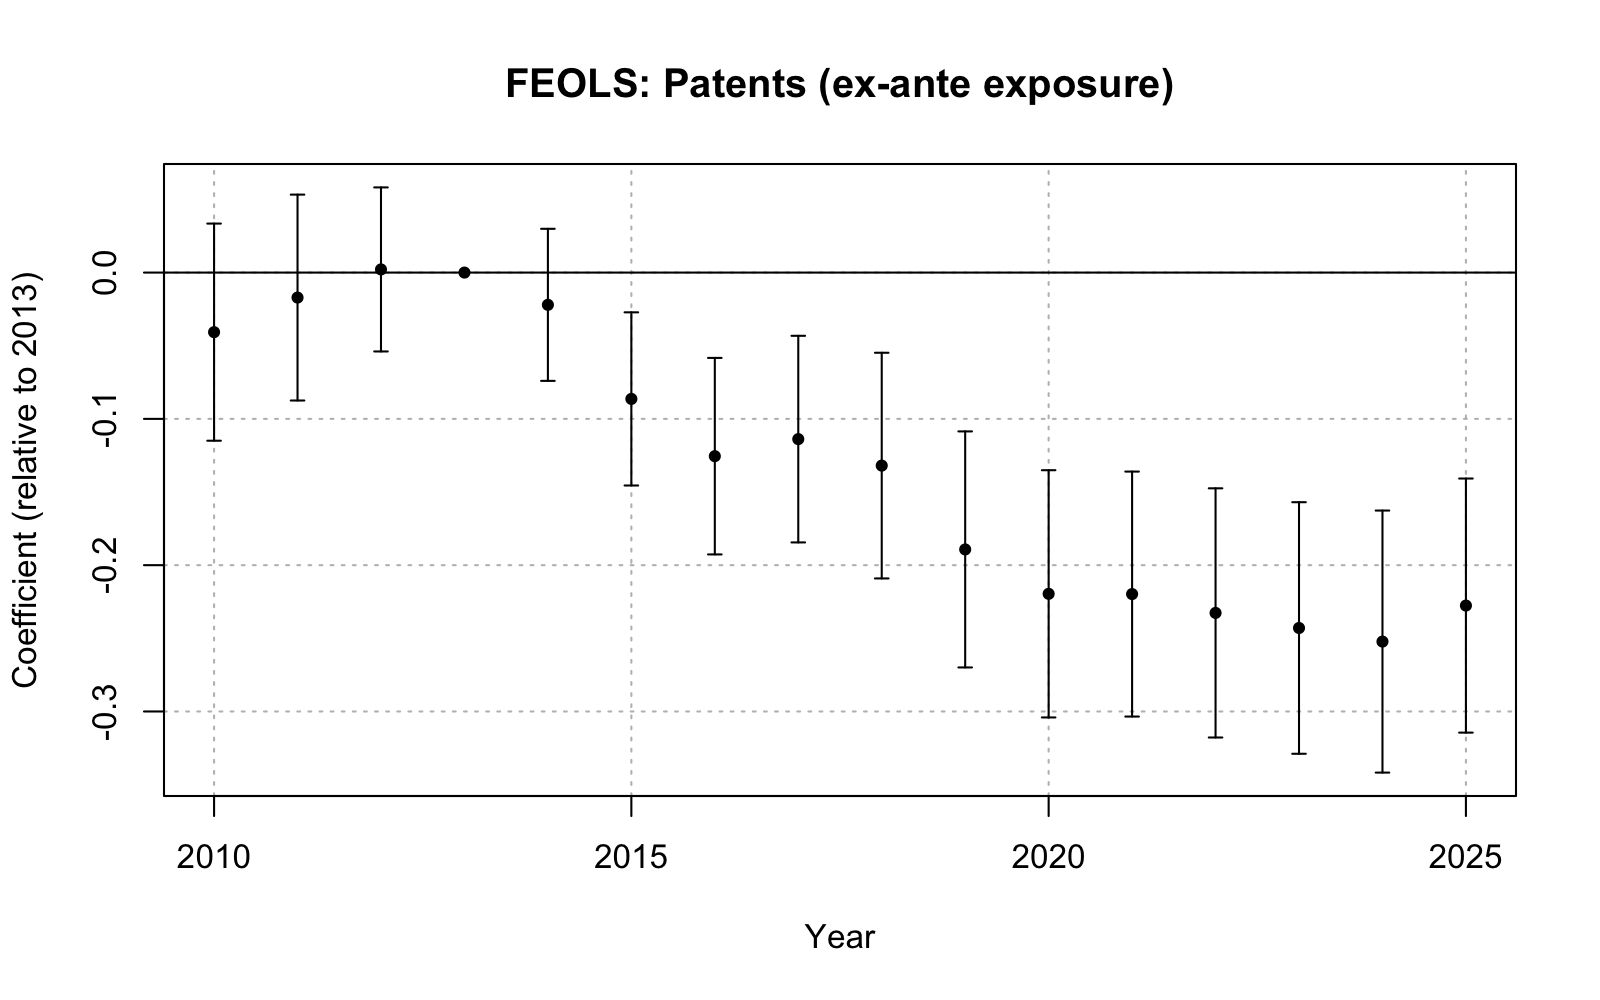
\includegraphics[width=\linewidth]{../output/RQ1/patent_feols_exante.png}
  \caption{FEOLS event study: patents, ex-ante Medicaid exposure}
  \label{fig:rq1_patent_feols_exante}
\end{figure}

\begin{figure}[!h]
  \centering
  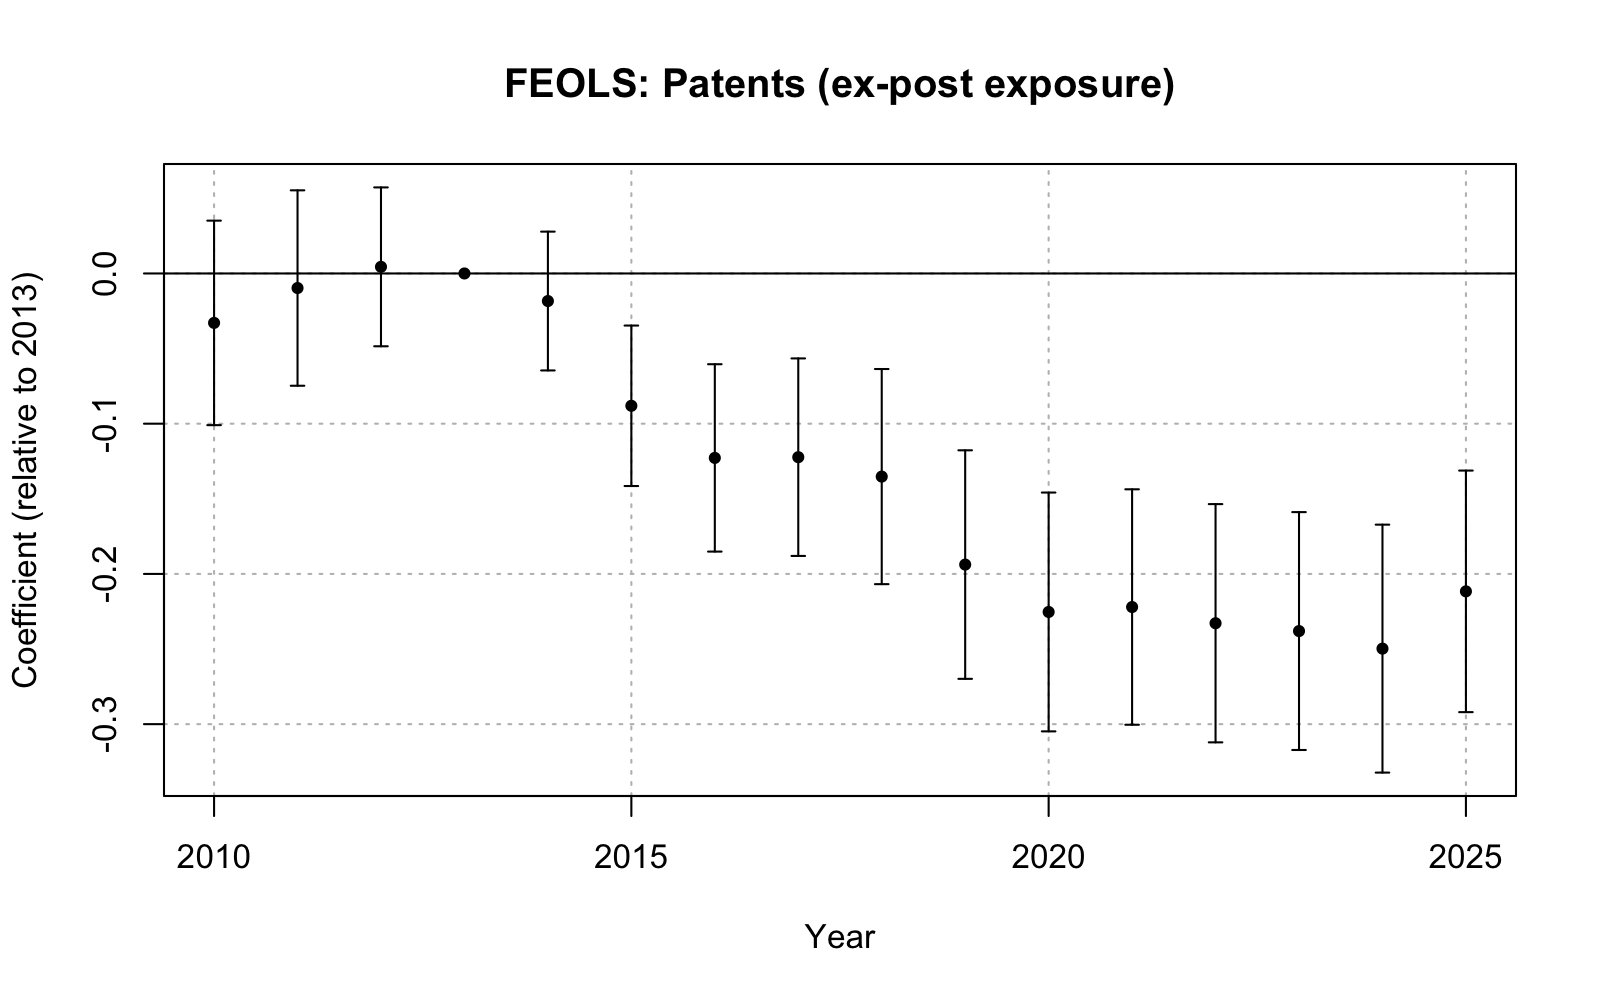
\includegraphics[width=\linewidth]{../output/RQ1/patent_feols_expost.png}
  \caption{FEOLS event study: patents, ex-post Medicaid exposure}
  \label{fig:rq1_patent_feols_expost}
\end{figure}

\begin{figure}[!h]
  \centering
  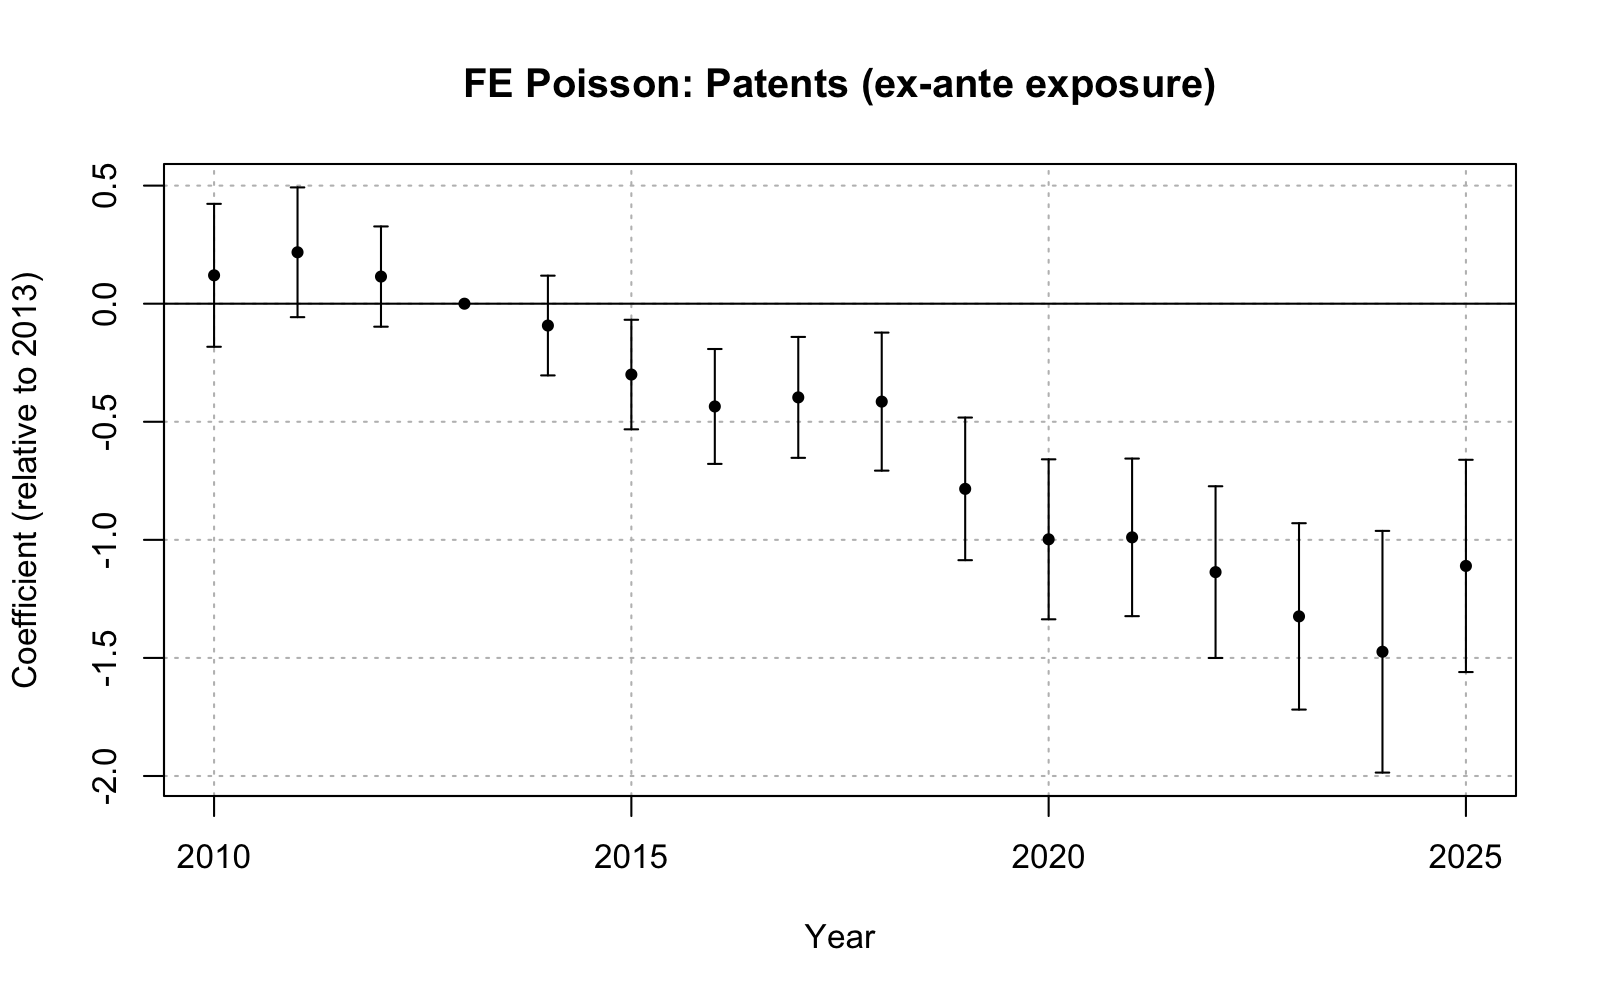
\includegraphics[width=\linewidth]{../output/RQ1/patent_poi_exante.png}
  \caption{FE Poisson event study: patents, ex-ante Medicaid exposure}
  \label{fig:rq1_patent_poi_exante}
\end{figure}

\begin{figure}[!h]
  \centering
  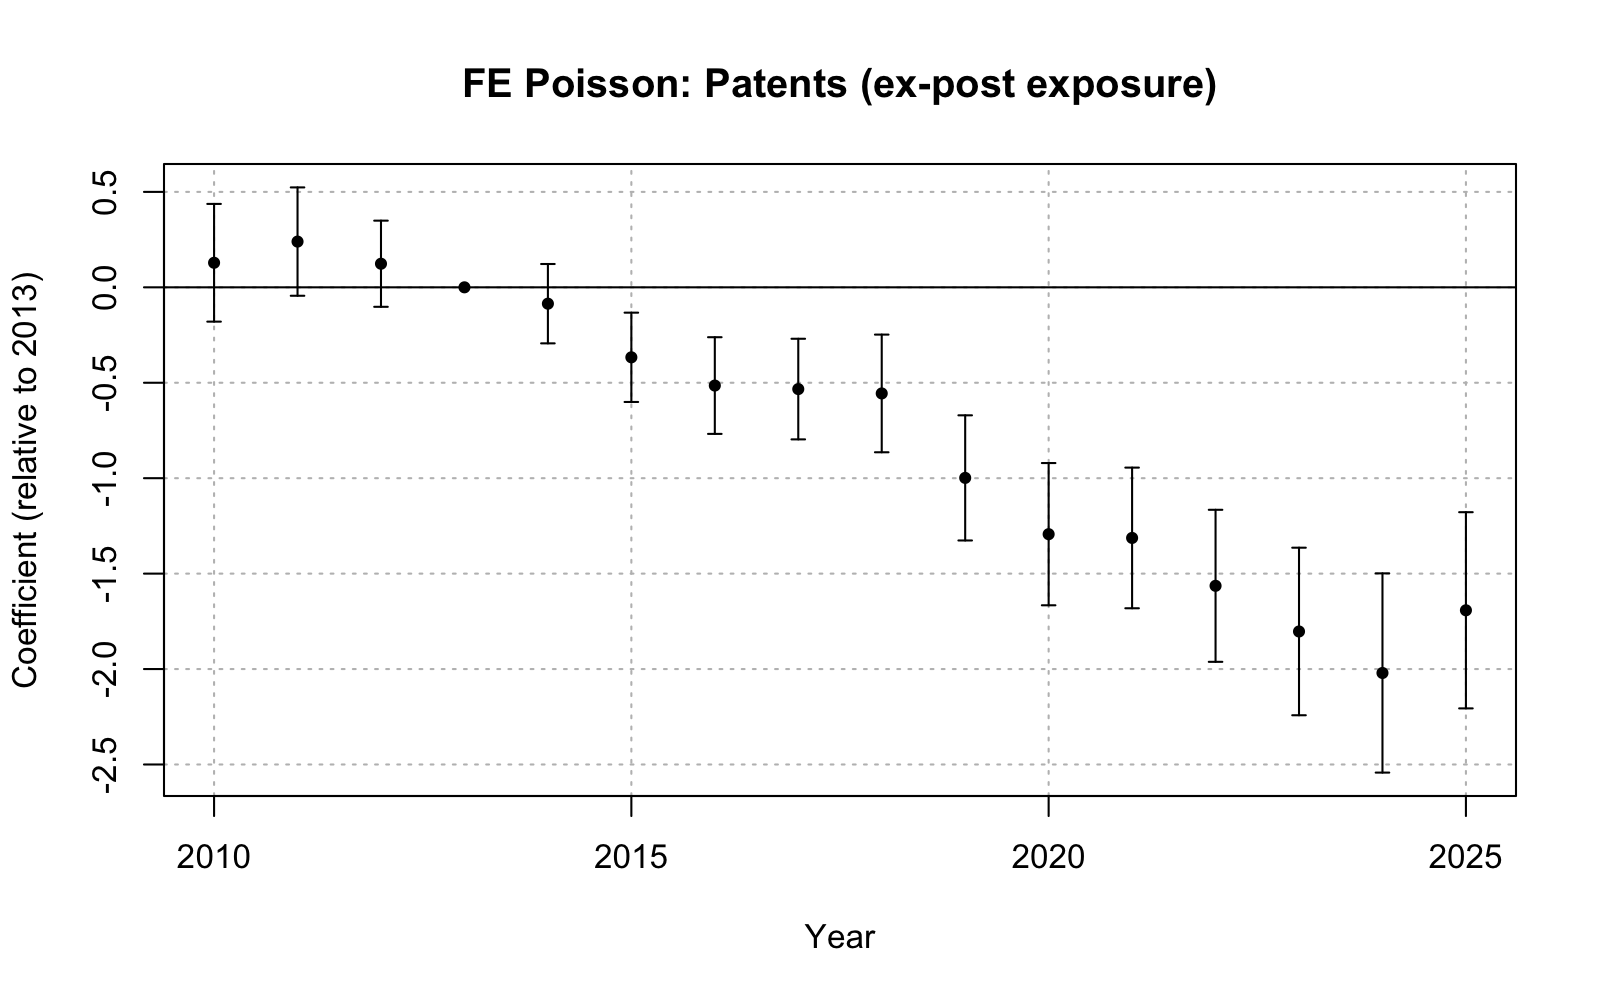
\includegraphics[width=\linewidth]{../output/RQ1/patent_poi_expost.png}
  \caption{FE Poisson event study: patents, ex-post Medicaid exposure}
  \label{fig:rq1_patent_poi_expost}
\end{figure}

\clearpage
\begingroup\footnotesize
\input{../output/RQ1/patent_models.tex}
\endgroup

\clearpage

\subsection{FDA Approvals}

\begin{figure}[!h]
  \centering
  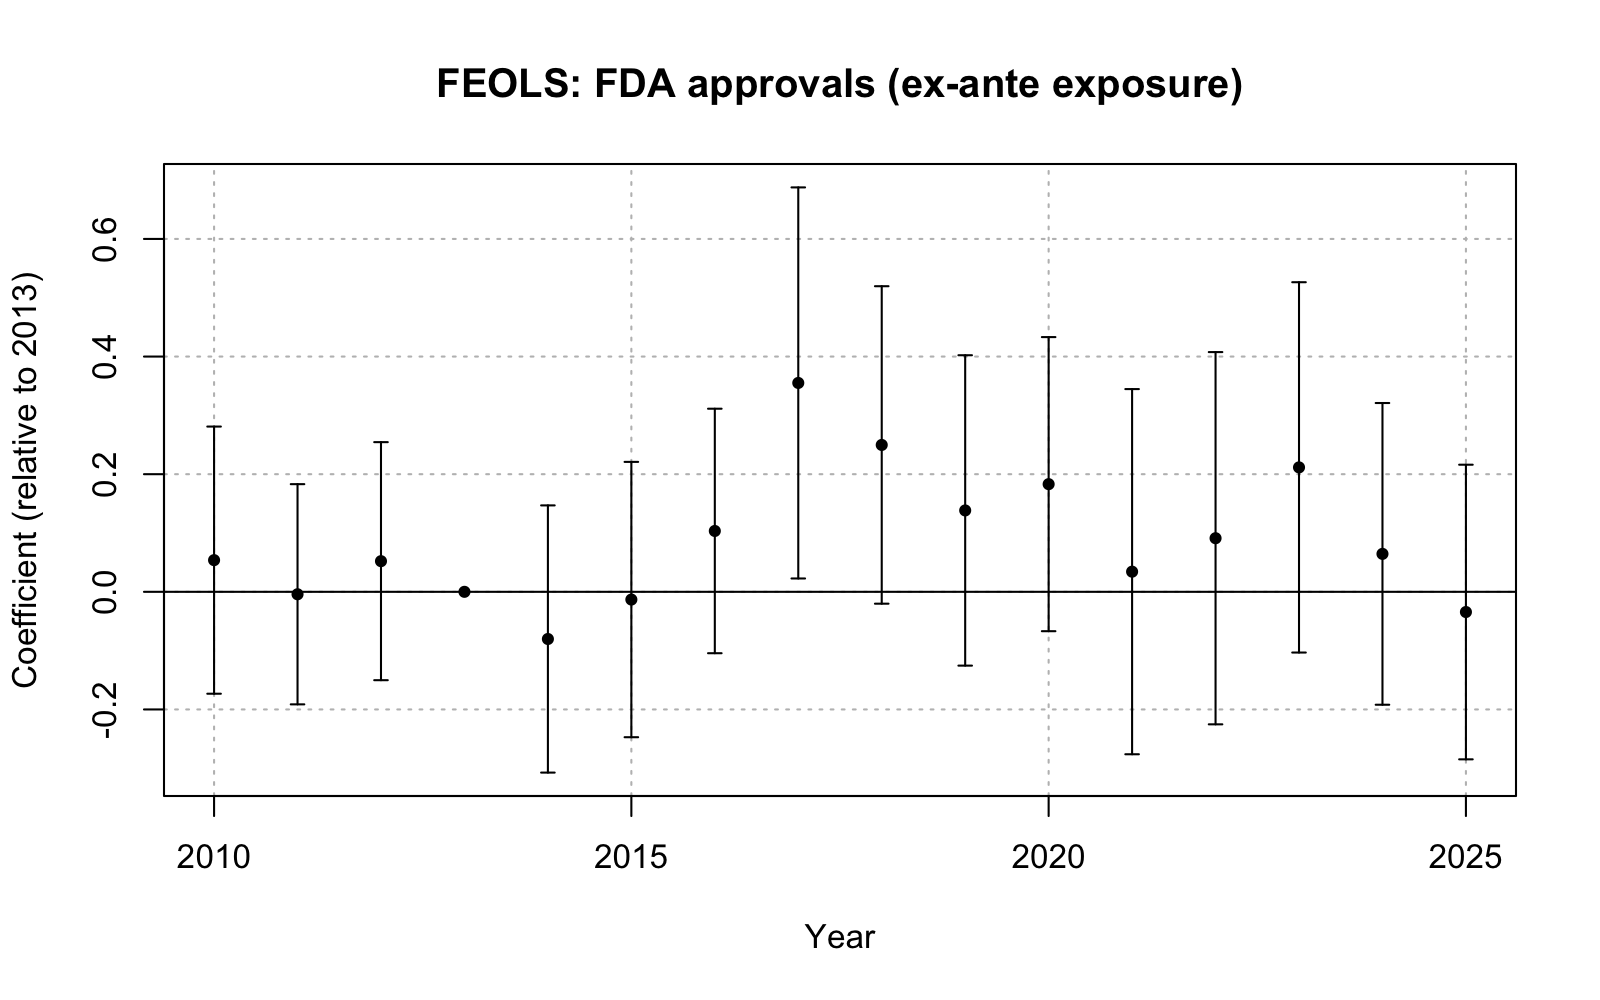
\includegraphics[width=\linewidth]{../output/RQ1/fda_feols_exante.png}
  \caption{FEOLS event study: FDA approvals, ex-ante Medicaid exposure}
  \label{fig:rq1_fda_feols_exante}
\end{figure}

\begin{figure}[!h]
  \centering
  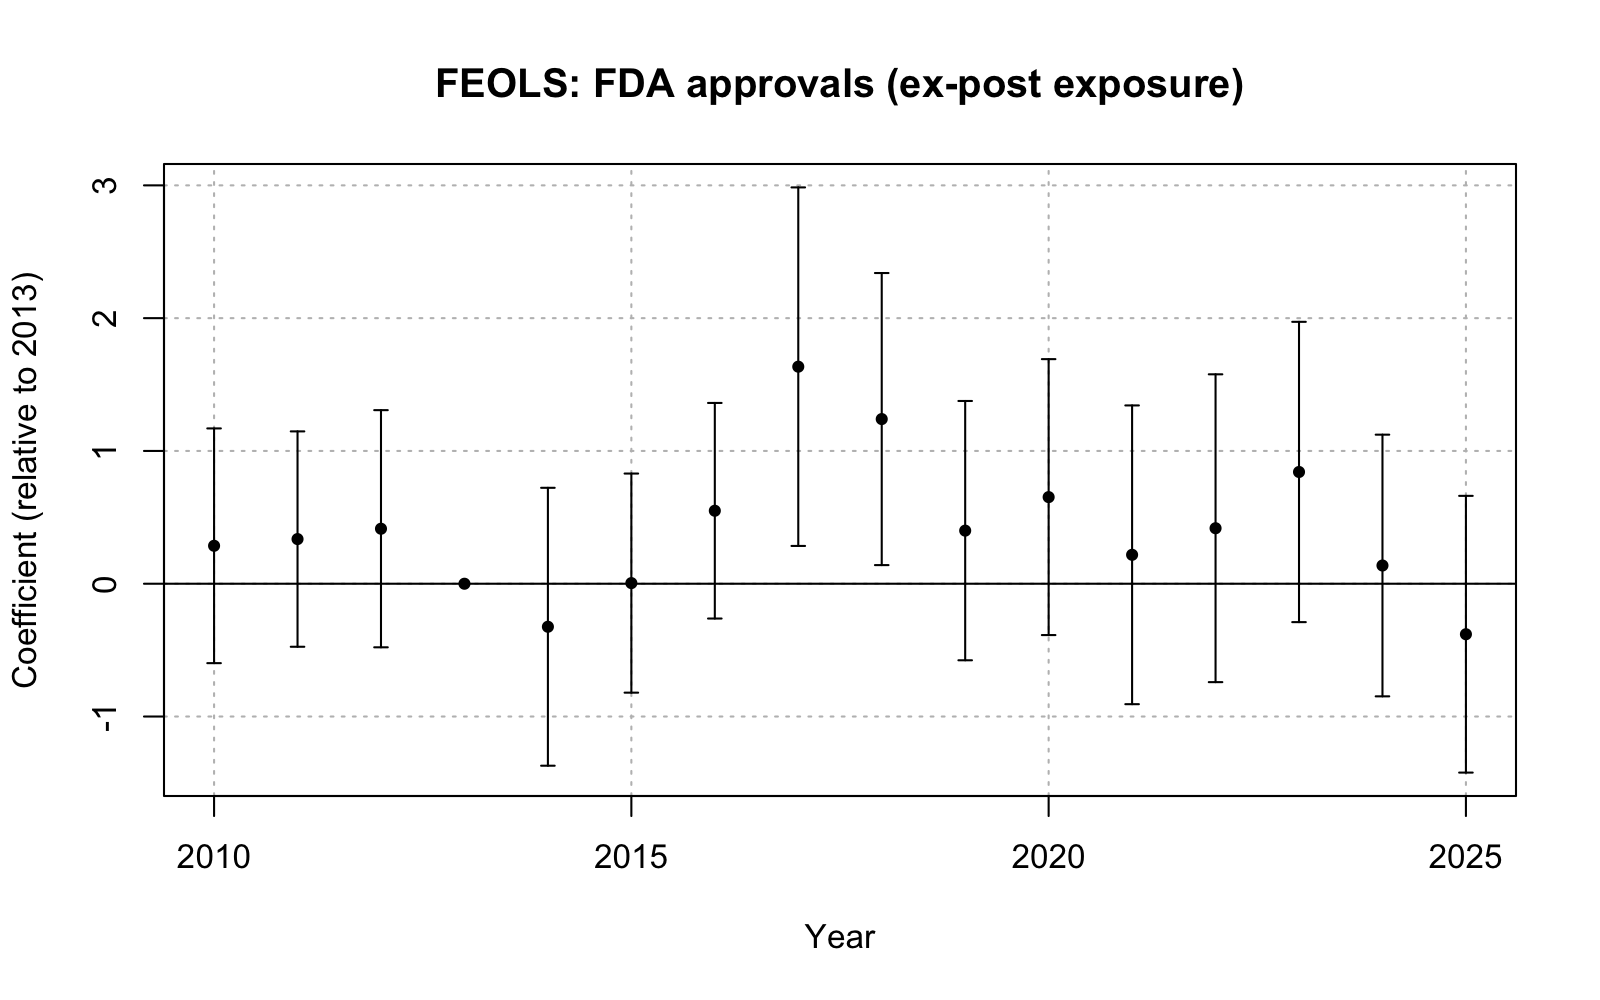
\includegraphics[width=\linewidth]{../output/RQ1/fda_feols_expost.png}
  \caption{FEOLS event study: FDA approvals, ex-post Medicaid exposure}
  \label{fig:rq1_fda_feols_expost}
\end{figure}

\begin{figure}[!h]
  \centering
  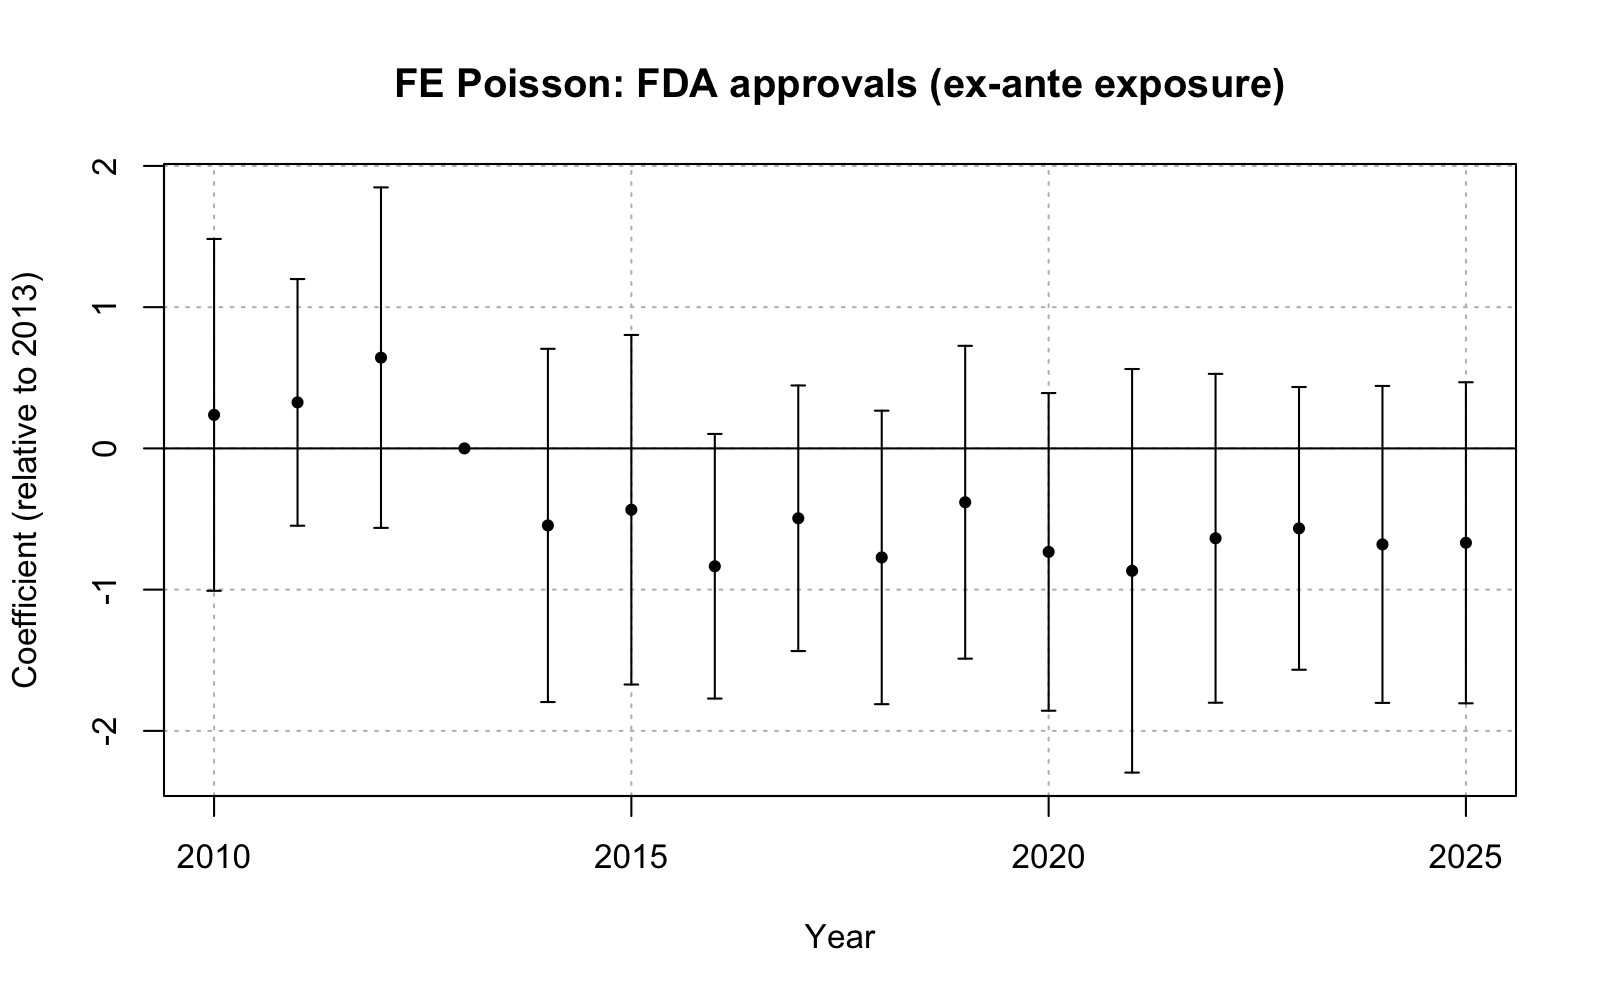
\includegraphics[width=\linewidth]{../output/RQ1/fda_poi_exante.png}
  \caption{FE Poisson event study: FDA approvals, ex-ante Medicaid exposure}
  \label{fig:rq1_fda_poi_exante}
\end{figure}

\begin{figure}[!h]
  \centering
  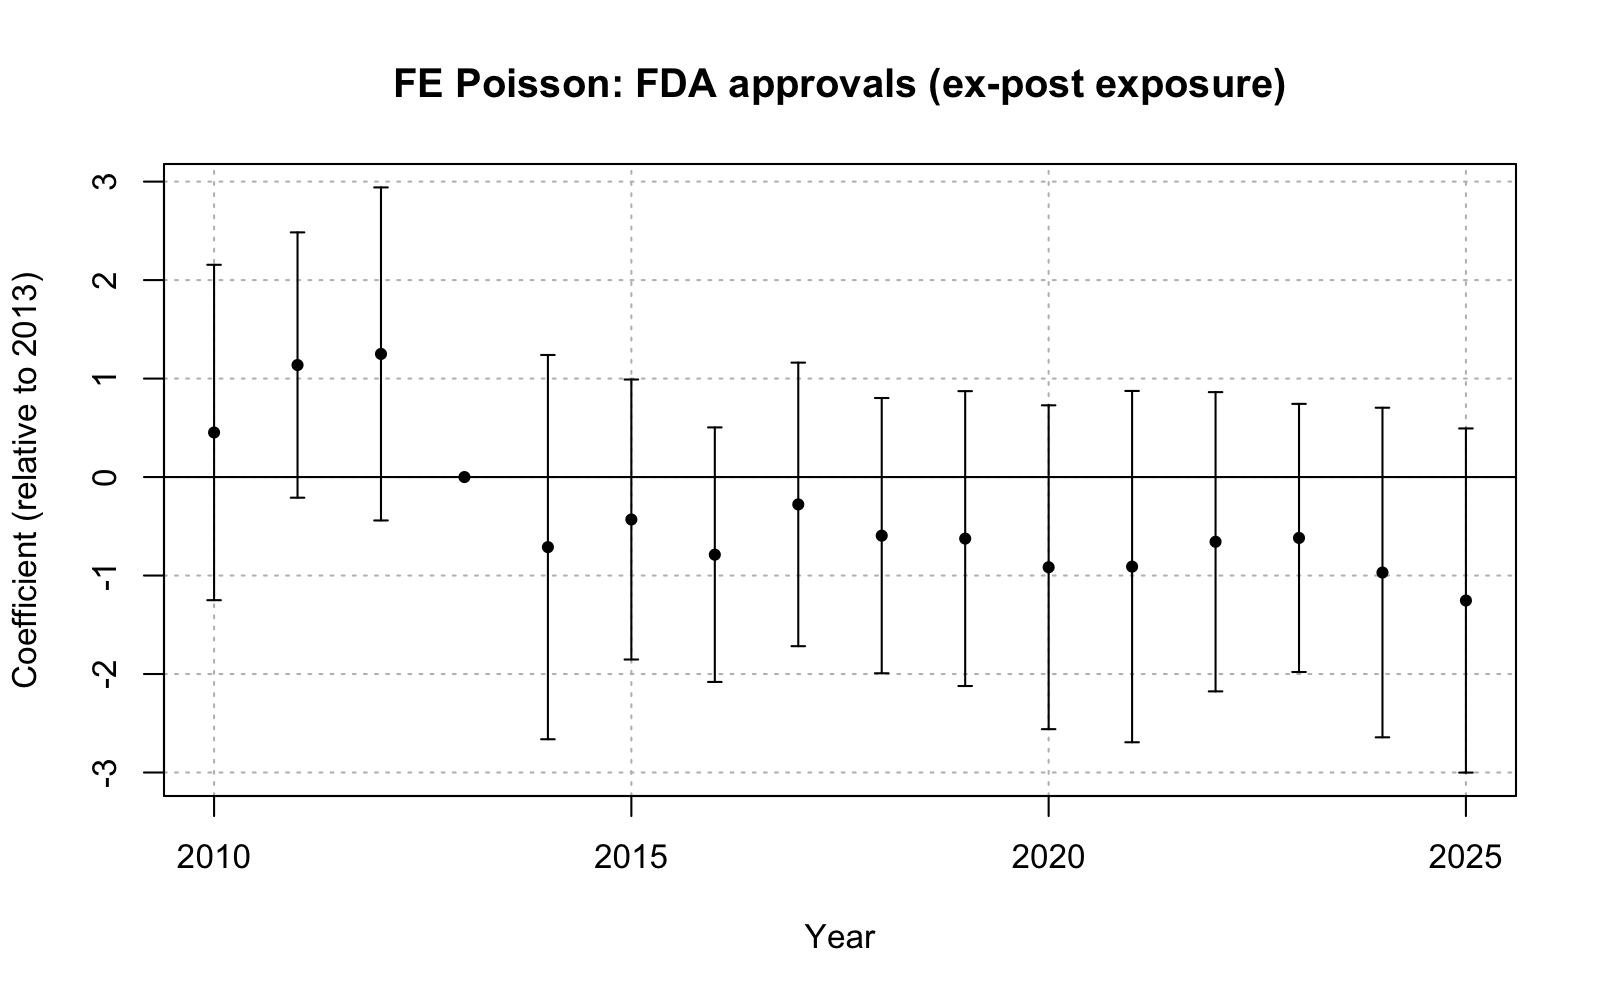
\includegraphics[width=\linewidth]{../output/RQ1/fda_poi_expost.png}
  \caption{FE Poisson event study: FDA approvals, ex-post Medicaid exposure}
  \label{fig:rq1_fda_poi_expost}
\end{figure}

\clearpage
\begingroup\footnotesize
\input{../output/RQ1/fda_models.tex}
\endgroup

\clearpage

% -----------------------------------------------------------------------
\section{RQ2: Medicaid Demand and PDL Exposure}
% -----------------------------------------------------------------------

\subsection{Patents}

\begin{figure}[!h]
  \centering
  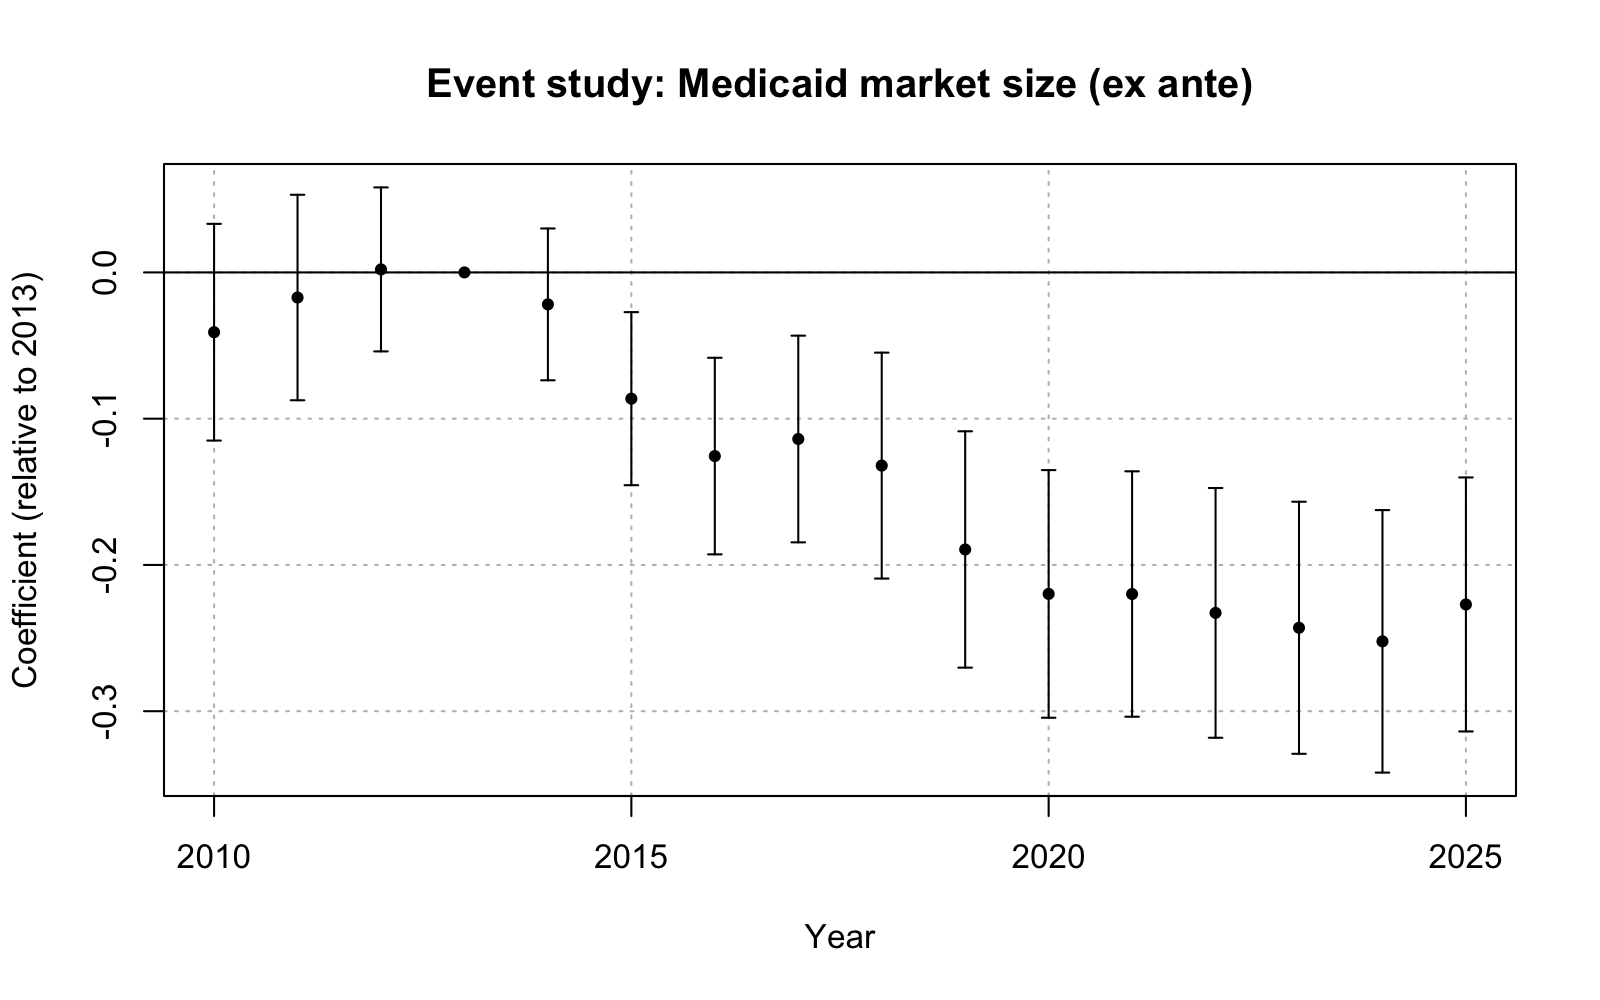
\includegraphics[width=\linewidth]{../output/RQ2/patent_feols_exante_medicaid.png}
  \caption{FEOLS event study: patents, Medicaid exposure (ex-ante)}
  \label{fig:rq2_patent_feols_exante_medicaid}
\end{figure}

\begin{figure}[!h]
  \centering
  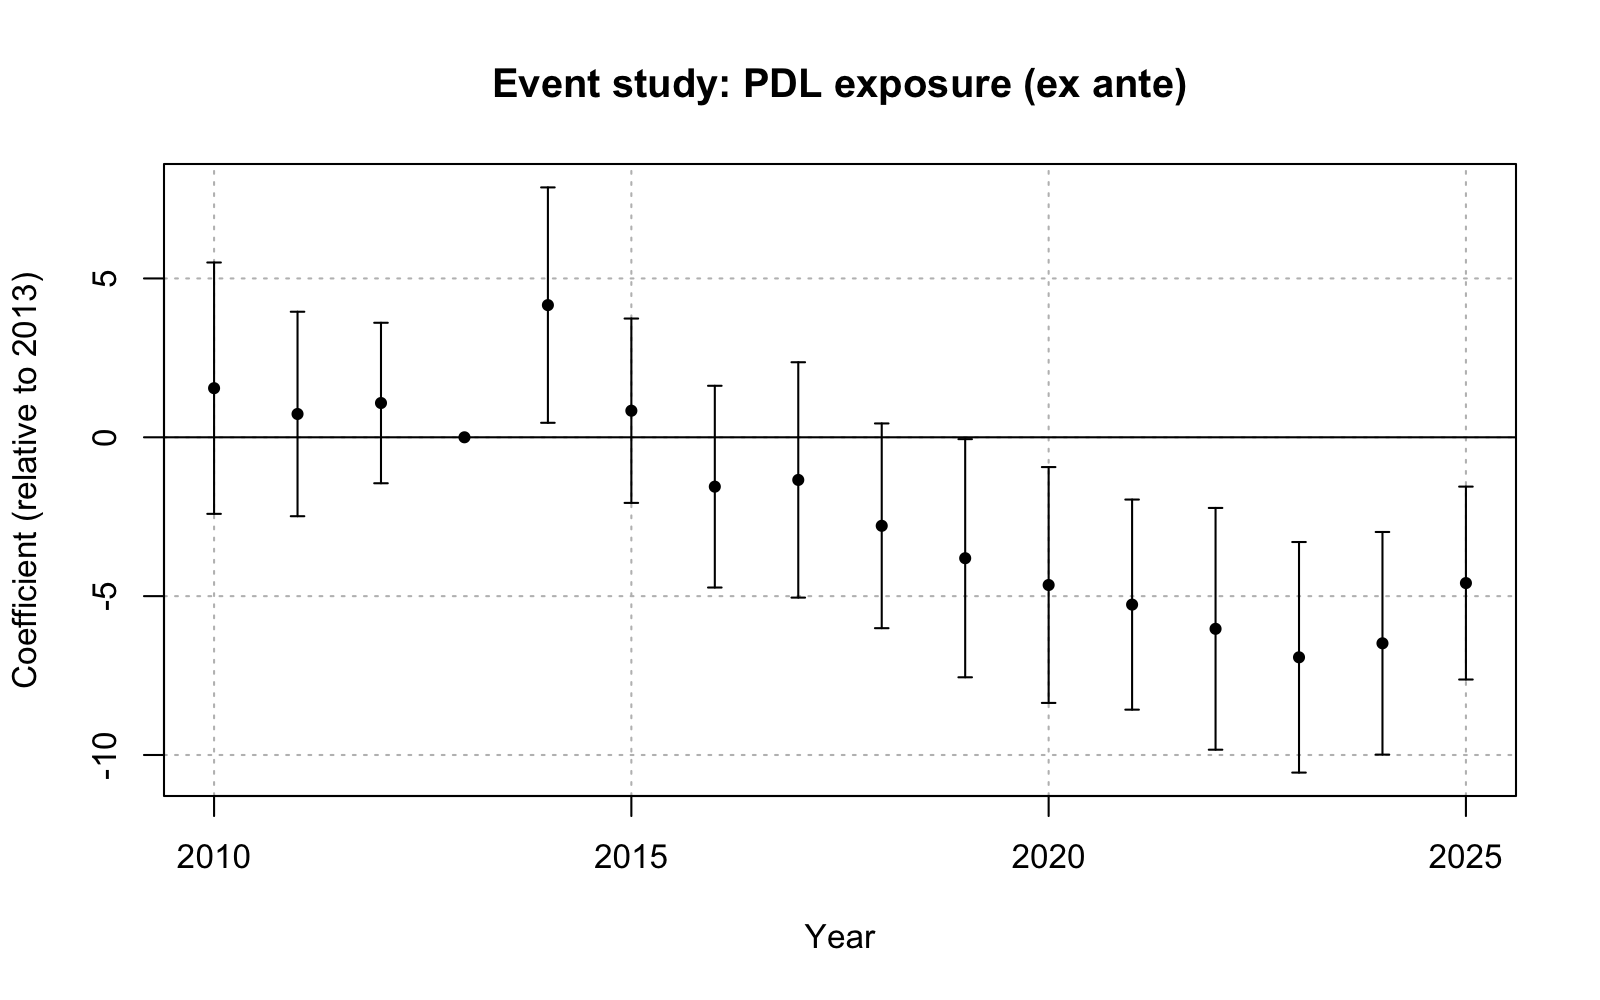
\includegraphics[width=\linewidth]{../output/RQ2/patent_feols_exante_pdl.png}
  \caption{FEOLS event study: patents, PDL exposure (ex-ante)}
  \label{fig:rq2_patent_feols_exante_pdl}
\end{figure}

\begin{figure}[!h]
  \centering
  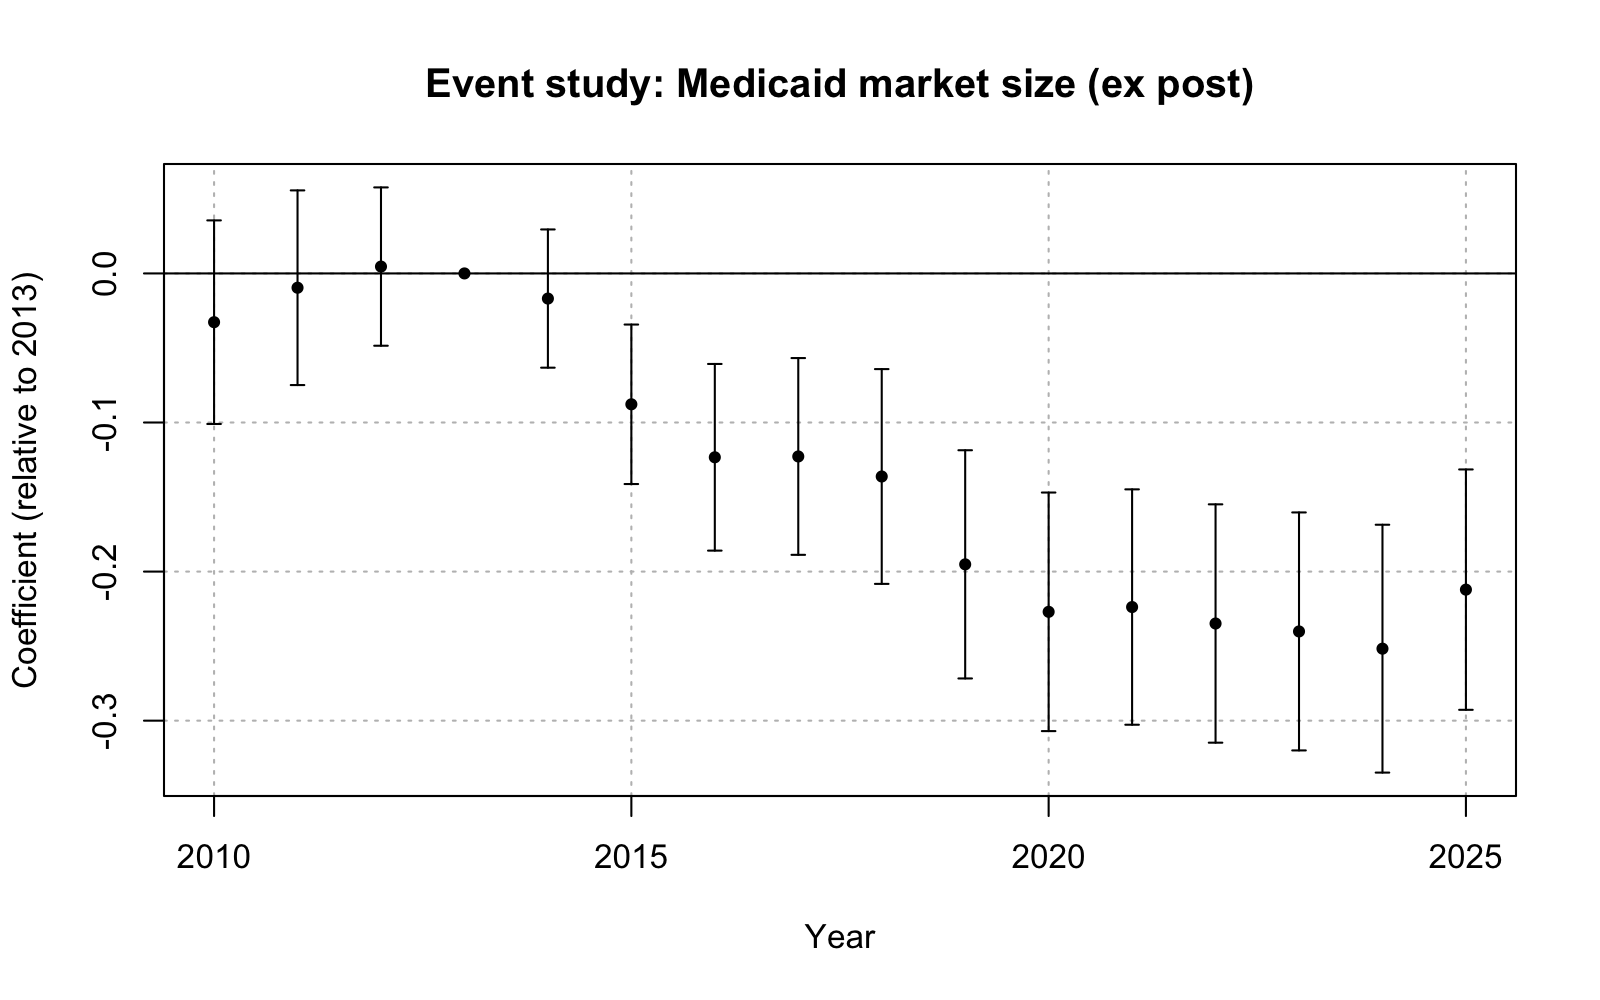
\includegraphics[width=\linewidth]{../output/RQ2/patent_feols_expost_medicaid.png}
  \caption{FEOLS event study: patents, Medicaid exposure (ex-post)}
  \label{fig:rq2_patent_feols_expost_medicaid}
\end{figure}

\begin{figure}[!h]
  \centering
  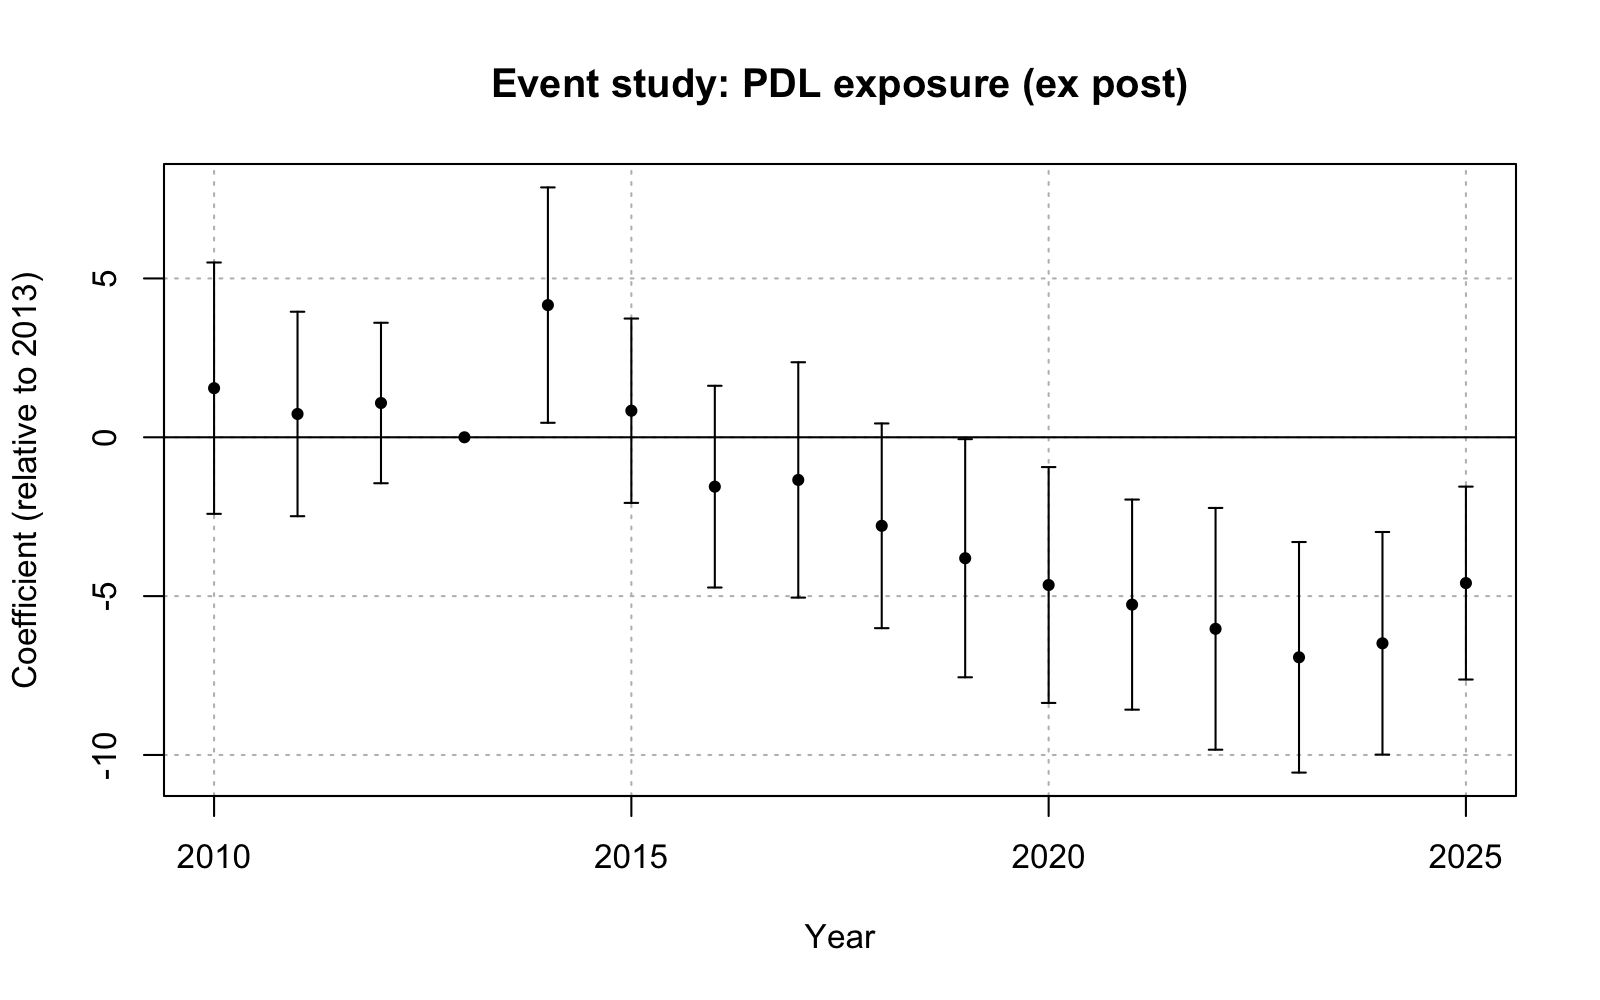
\includegraphics[width=\linewidth]{../output/RQ2/patent_feols_expost_pdl.png}
  \caption{FEOLS event study: patents, PDL exposure (ex-post)}
  \label{fig:rq2_patent_feols_expost_pdl}
\end{figure}

\clearpage
\begingroup\footnotesize
\input{../output/RQ2/patent_models.tex}
\endgroup

\clearpage

\subsection{FDA Approvals}

\begin{figure}[!h]
  \centering
  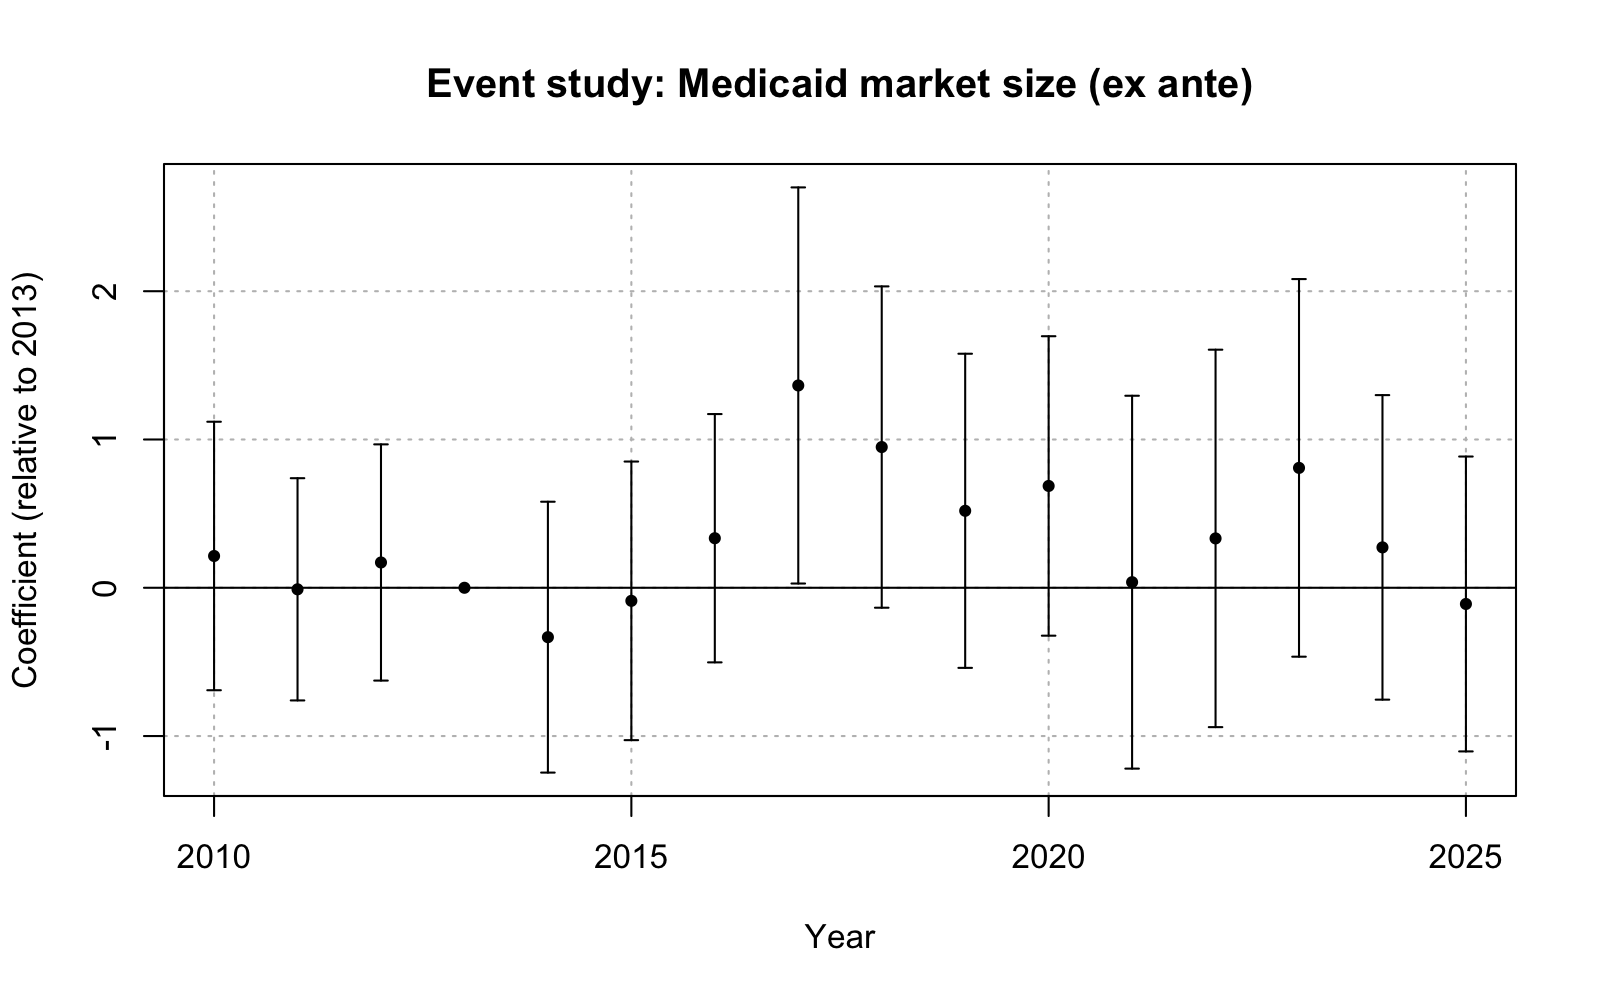
\includegraphics[width=\linewidth]{../output/RQ2/fda_feols_exante_medicaid.png}
  \caption{FEOLS event study: FDA approvals, Medicaid exposure (ex-ante)}
  \label{fig:rq2_fda_feols_exante_medicaid}
\end{figure}

\begin{figure}[!h]
  \centering
  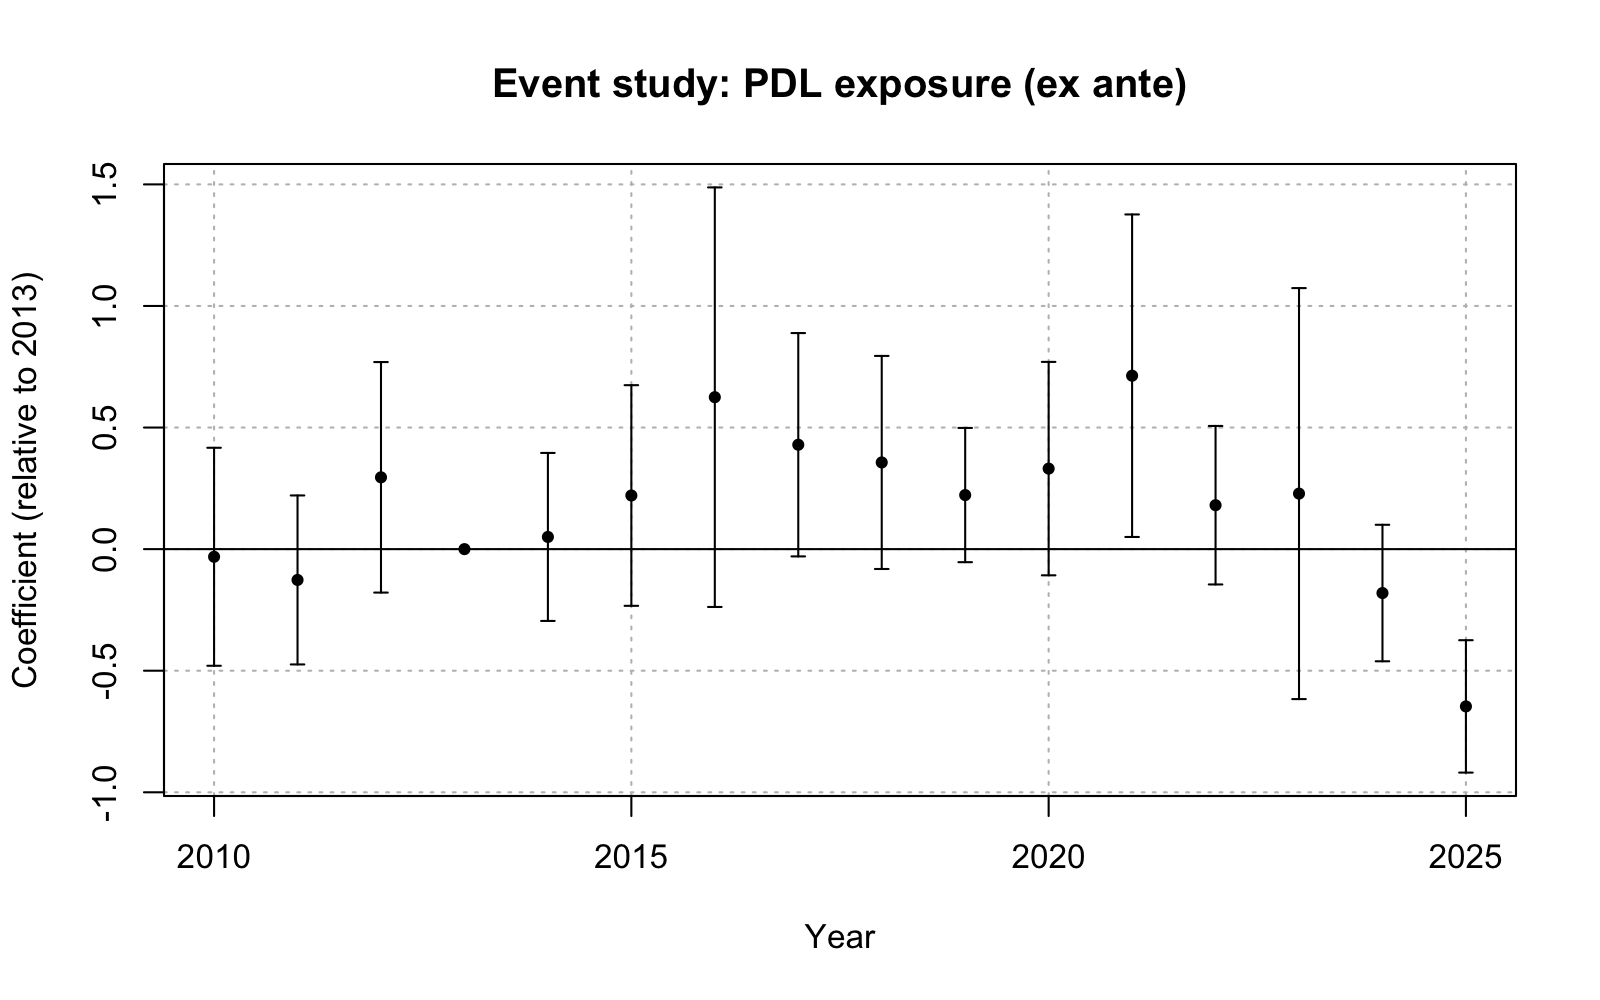
\includegraphics[width=\linewidth]{../output/RQ2/fda_feols_exante_pdl.png}
  \caption{FEOLS event study: FDA approvals, PDL exposure (ex-ante)}
  \label{fig:rq2_fda_feols_exante_pdl}
\end{figure}

\begin{figure}[!h]
  \centering
  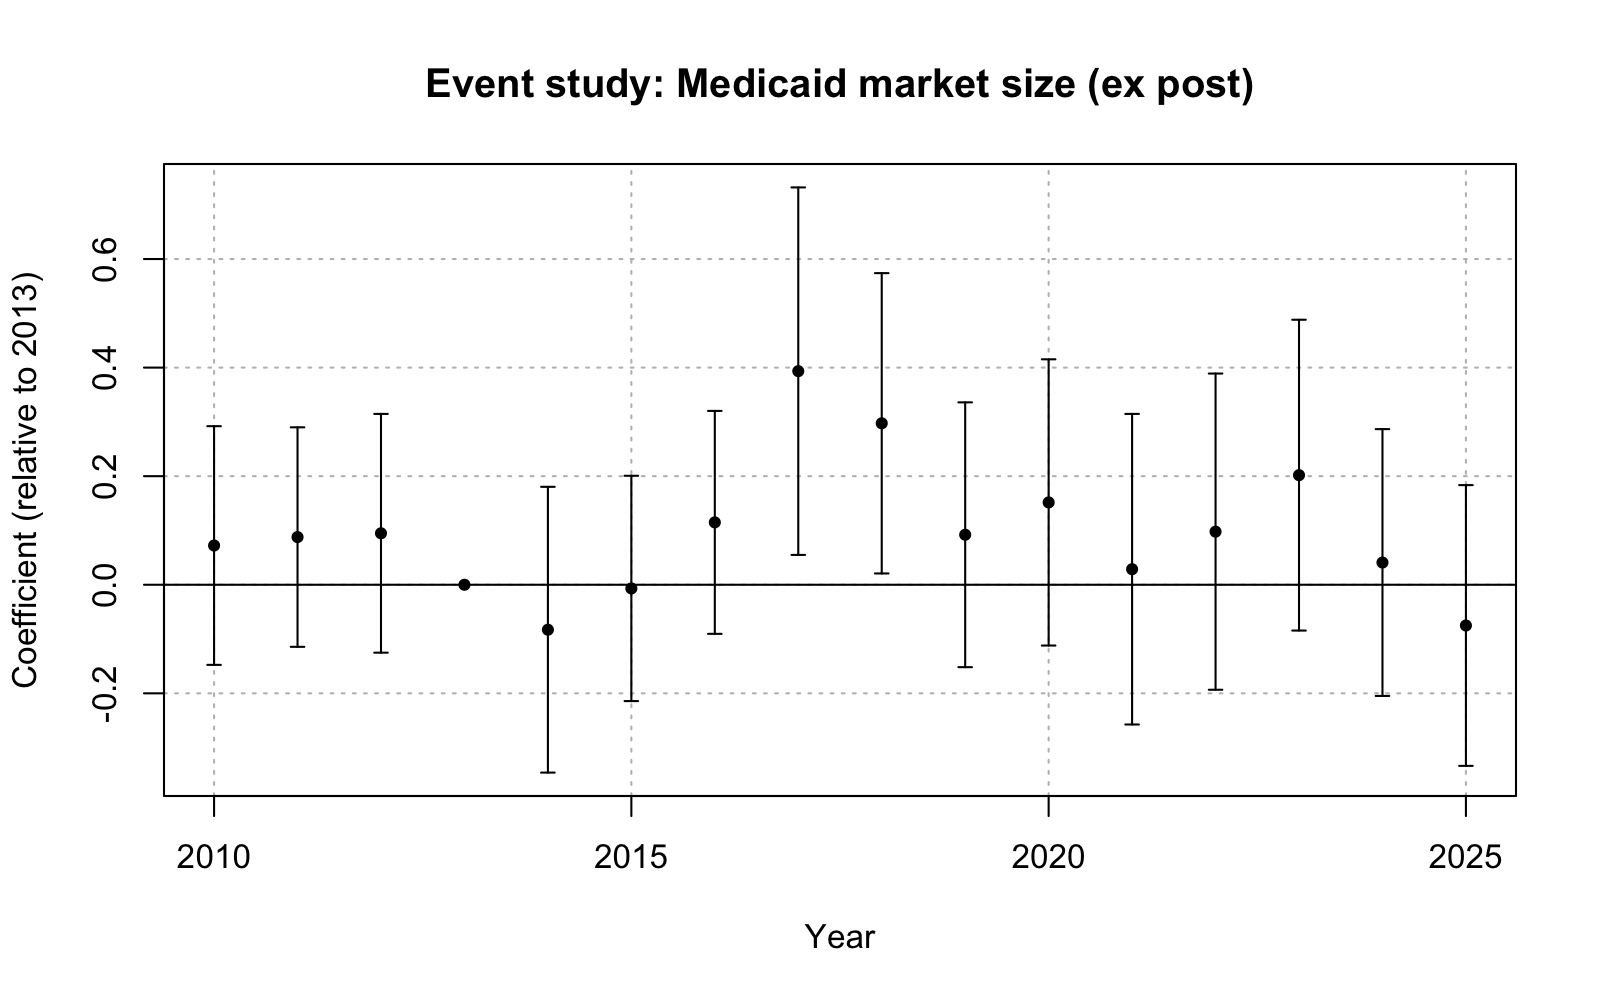
\includegraphics[width=\linewidth]{../output/RQ2/fda_feols_expost_medicaid.png}
  \caption{FEOLS event study: FDA approvals, Medicaid exposure (ex-post)}
  \label{fig:rq2_fda_feols_expost_medicaid}
\end{figure}

\begin{figure}[!h]
  \centering
  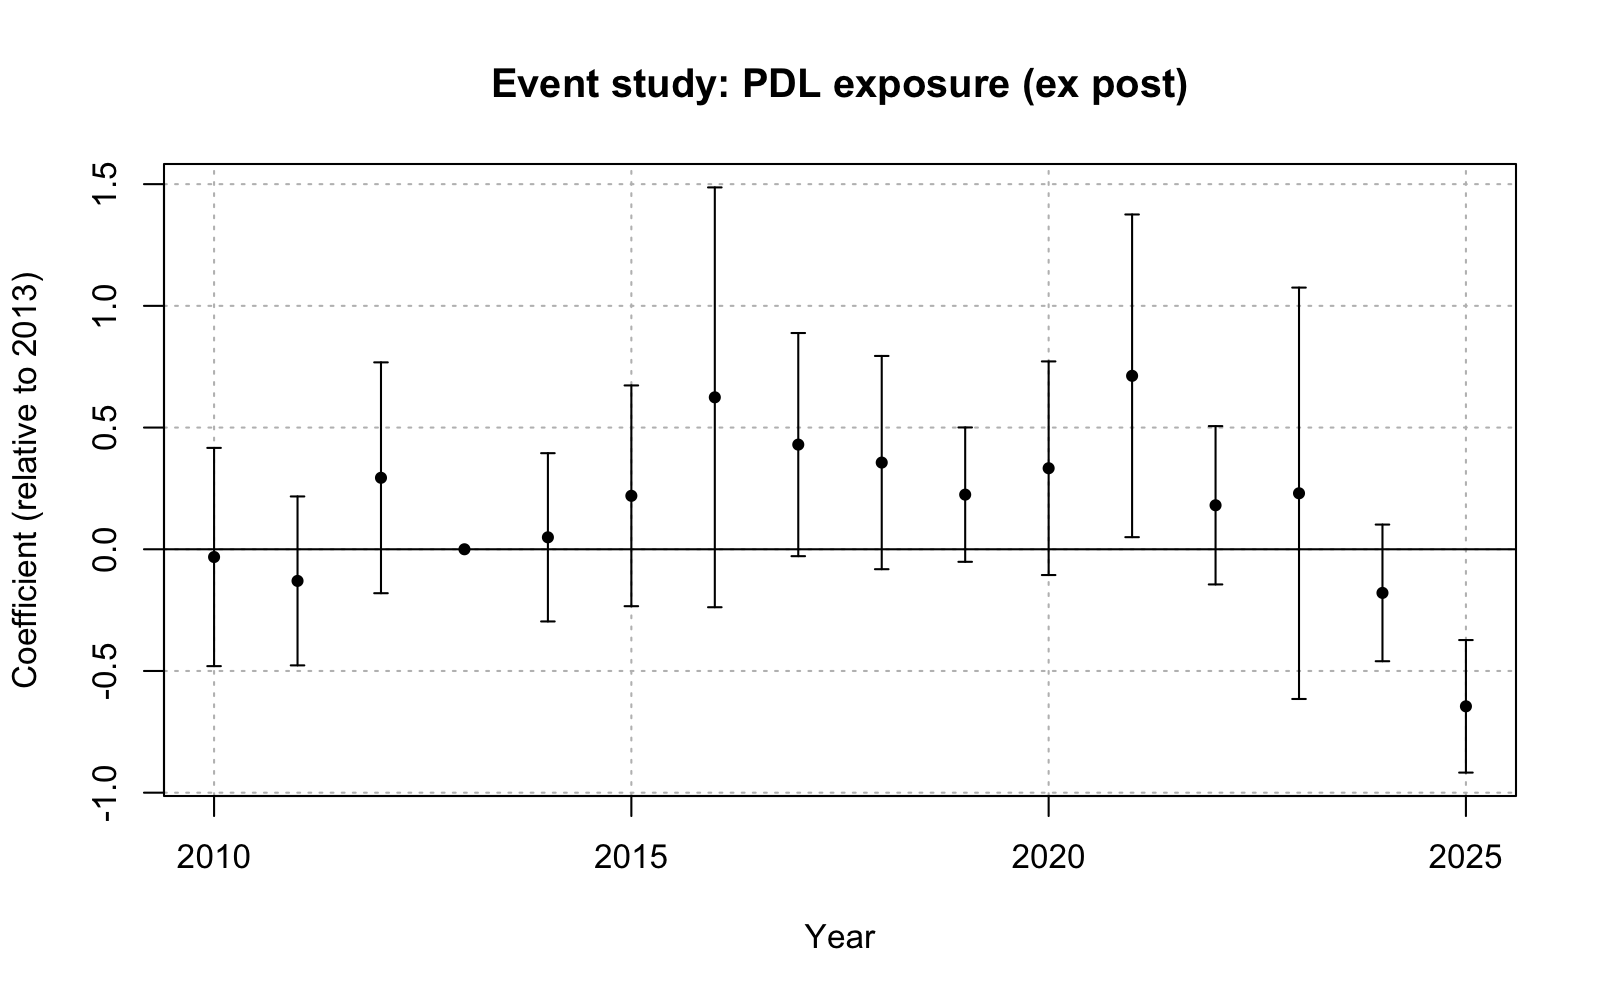
\includegraphics[width=\linewidth]{../output/RQ2/fda_feols_expost_pdl.png}
  \caption{FEOLS event study: FDA approvals, PDL exposure (ex-post)}
  \label{fig:rq2_fda_feols_expost_pdl}
\end{figure}

\clearpage
\begingroup\footnotesize
\input{../output/RQ2/fda_models.tex}
\endgroup

\clearpage

% -----------------------------------------------------------------------
\section{RQ3: Therapeutic-Class Heterogeneity}
% -----------------------------------------------------------------------

\subsection{Patents}

\begin{center}
\begingroup\footnotesize
\input{../output/RQ3/patent_models.tex}
\endgroup
\end{center}

\subsection{FDA Approvals}

\begin{center}
\begingroup\footnotesize
\input{../output/RQ3/fda_models.tex}
\endgroup
\end{center}

\clearpage

% -----------------------------------------------------------------------
\section{PDL Counterfactual Analysis}
% -----------------------------------------------------------------------

\begin{center}
\begingroup\footnotesize
\input{../output/PDL_counterfactual/pdl_counterfactual_models.tex}
\endgroup
\end{center}

\clearpage

\bibliographystyle{apalike}
\bibliography{references}

\end{document}

\documentclass[12pt]{article}
\usepackage{geometry}
\geometry{a4paper, portrait, margin=1in}

% --- Math Packages ---
\usepackage{amsmath}
\usepackage{amssymb}
\usepackage{amsfonts}
\usepackage{amsthm}

% --- Graphics & Diagrams ---
\usepackage{graphicx}
\usepackage{tikz}
\usetikzlibrary{shapes, arrows, positioning}

% --- Formatting ---
\usepackage{parskip}
\usepackage[hidelinks]{hyperref}
\usepackage{natbib}
\usepackage{enumitem}
\usepackage{booktabs}
\usepackage{caption}
\usepackage{float}
\usepackage{siunitx}
\usepackage{tabularray}
\UseTblrLibrary{booktabs, siunitx}
\pagestyle{plain}

% --- Allow talltblr to break across pages ---
\renewenvironment{table}[1][]{}{}

% --- Word count (requires compiling with --shell-escape) ---
\newcommand{\wordcount}{%
  \immediate\write18{texcount -sum -1 \jobname.tex 2>/dev/null | python3 -c "import sys; n=sys.stdin.read().strip(); print(f'{int(n):,}') if n.isdigit() else print('?')" > \jobname.wc}%
  \input{\jobname.wc}%
}

\title{MPhil Thesis: Robustness and Sensitivity Analysis}
\author{Mohammad-Shah Karim}
\date{May 2026}

\begin{document}

\maketitle

\begin{center}
  \small Word count: \wordcount
\end{center}

\tableofcontents

\newpage

% -----------------------------------------------------------------------
\section{Robustness and Sensitivity Analysis}
% -----------------------------------------------------------------------

The baseline results are estimated using FEOLS with an ex-ante Medicaid market share measure as a proxy for firm-class exposure to the Medicaid reform. This section examines the sensitivity of these findings to alternative specifications, estimation methods, and treatment of the continuous exposure variable. Each research question is addressed in turn.

% -----------------------------------------------------------------------
\subsection{RQ1: Overall Innovation Response}
% -----------------------------------------------------------------------

\subsubsection{Ex-Post Medicaid Exposure}

The baseline specification uses pre-expansion Medicaid market shares to measure treatment intensity. Ex-post market shares are constructed from realised the Medicaid prescription shares in 2014-2015 as an alternative measure of exposure to the ACA. The window for ex-post shares is restricted to the first two years of the reform in order to capture initial shifts in demand without extending into periods where endogenous response in firm entry or prescribing behaviour, may contaminate the exposure measure. Estimates using ex-post exposure act purely as a robustness check since the measure would still reflect the actual post-expansion demand environment as opposed to being a predetermined exposure measure.

Under the estimated ex-post measure, the patent coefficients are nearly identical to the ex-ante estimates. The pre-expansion coefficients remain small and insignificant, highlighting robustness to the parallel trends assumption while the post-reform coefficients follow the same gradual negative trajectory, growing from $-0.088$ in 2015 to $-0.250$ by 2024 before dropping slightly to $-0.212$ in 2025. These estimates are consistent with the ex-ante result, which also has a 2024 peak at $-0.252$. Similarly, the coefficients for FDA approvals are also in line with the baseline specification, where the coefficients are largely statistically insignificant with the exception of 2017 and 2019, while having no clear directional pattern. The alignment between the ex-ante and ex-post results therefore indicates that the findings are orthogonal to the choice of exposure measure.

\begin{figure}[!h]
  \centering
  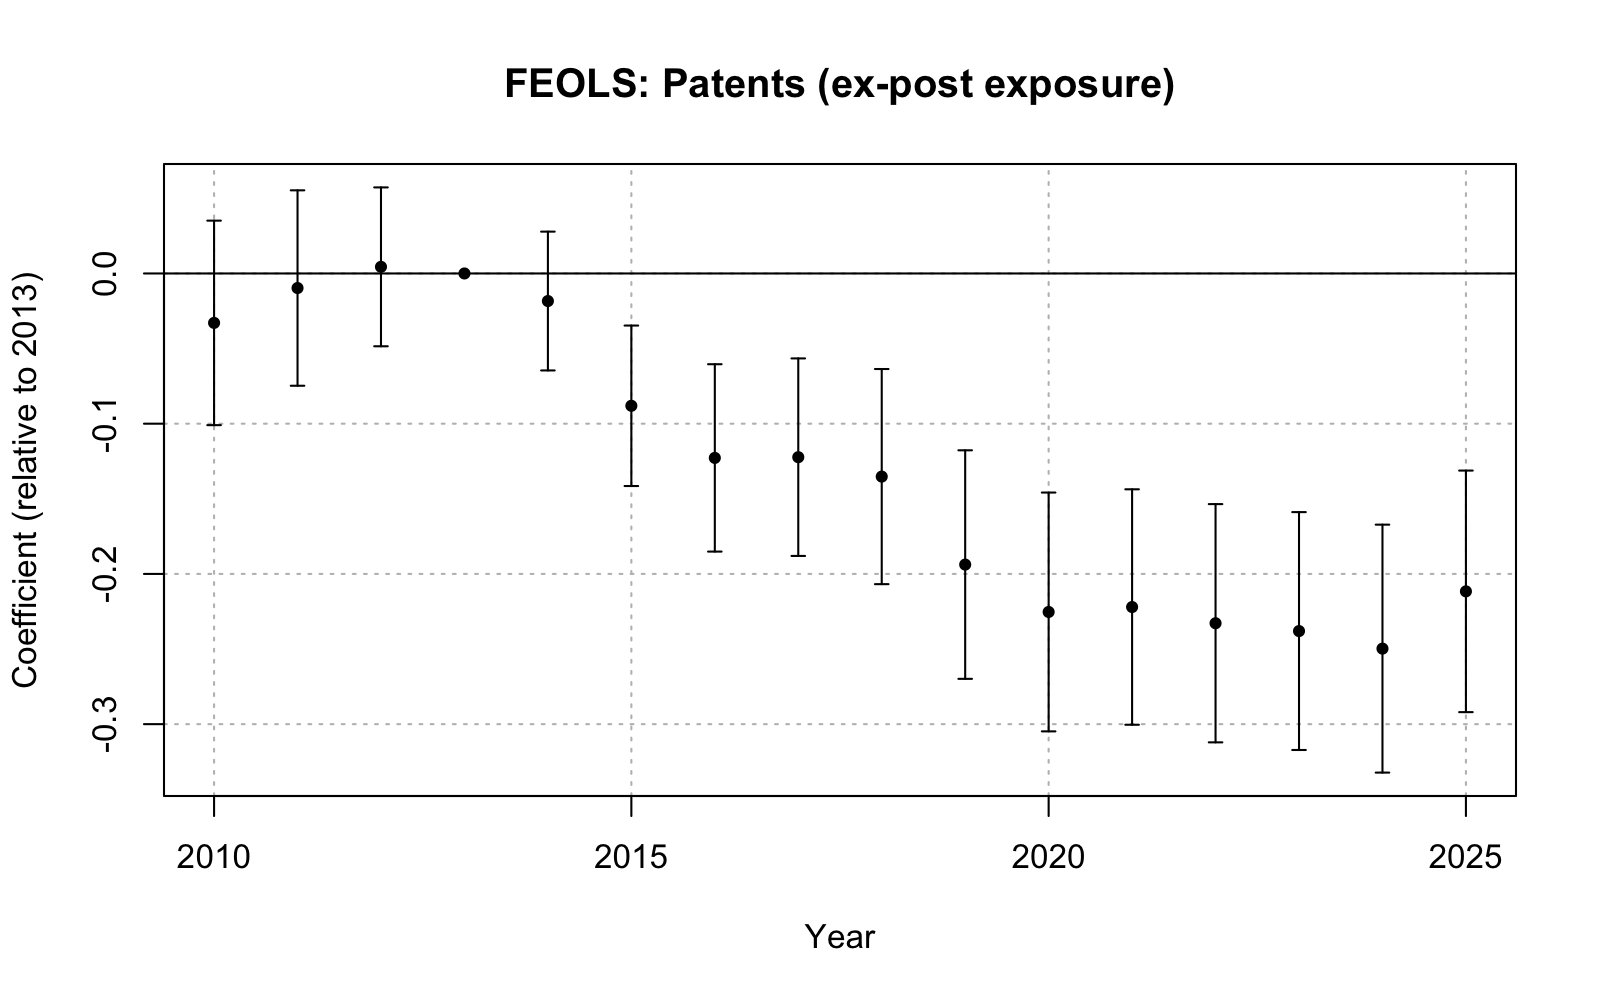
\includegraphics[width=\linewidth]{../output/RQ1/patent_feols_expost.png}
  \caption{FEOLS event study: patents, ex-post Medicaid exposure}
  \label{fig:rob_rq1_patent_feols_expost}
\end{figure}

\begin{figure}[!h]
  \centering
  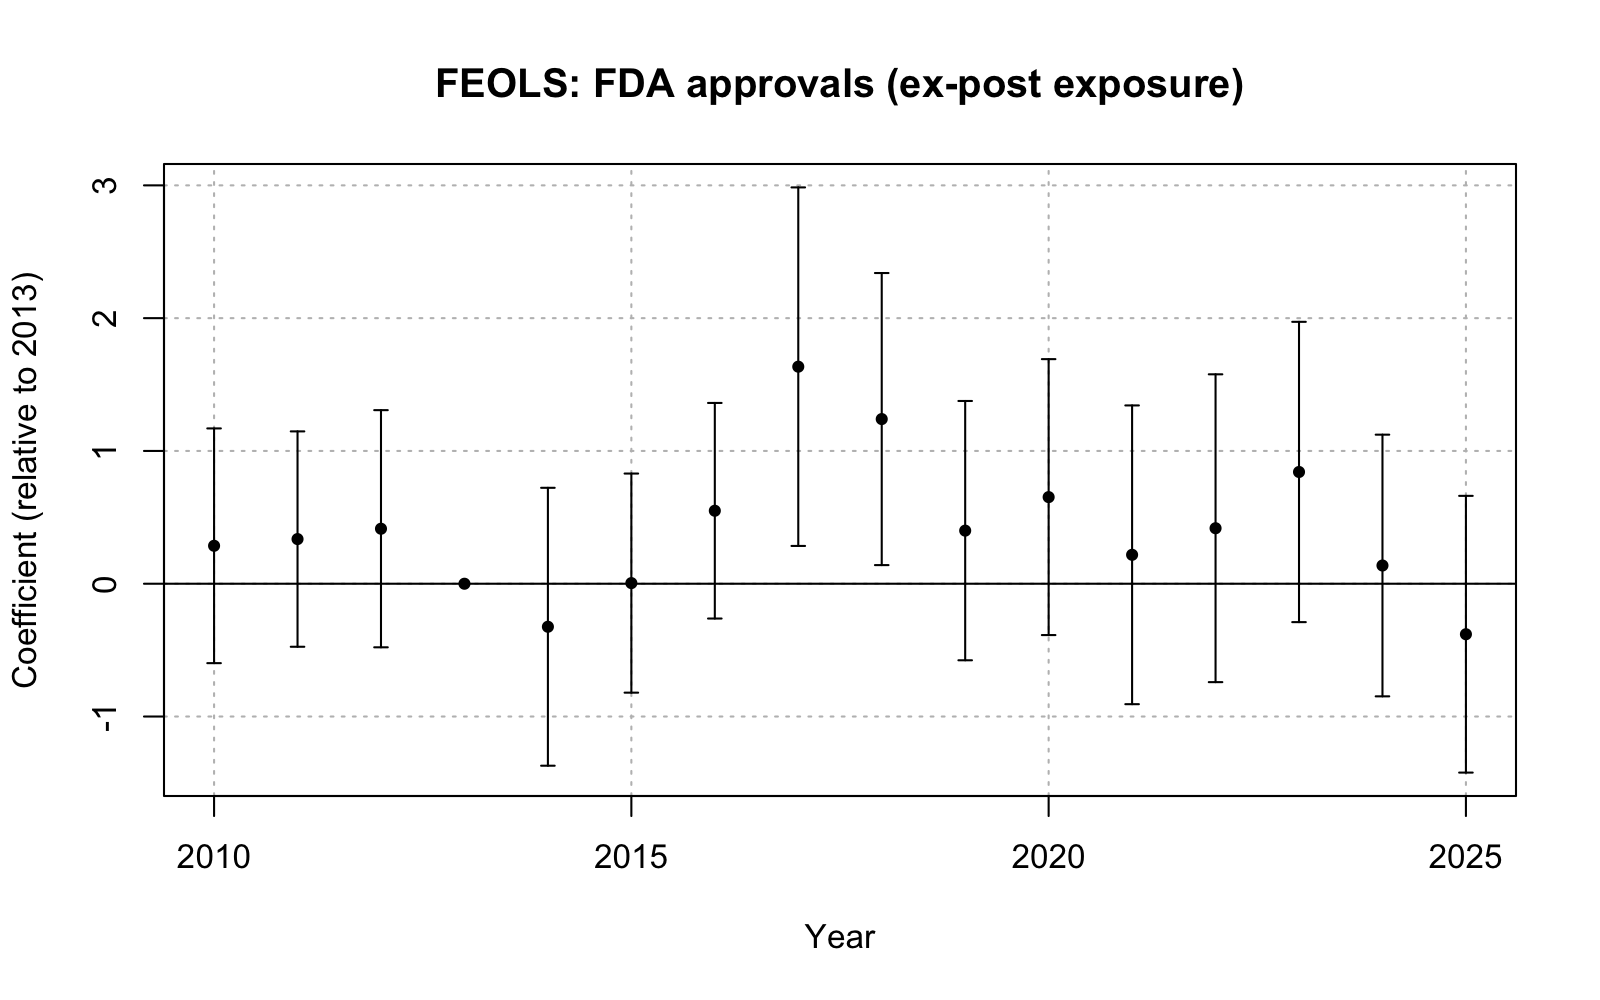
\includegraphics[width=\linewidth]{../output/RQ1/fda_feols_expost.png}
  \caption{FEOLS event study: FDA approvals, ex-post Medicaid exposure}
  \label{fig:rob_rq1_fda_feols_expost}
\end{figure}

\clearpage

\subsubsection{FE Poisson Estimation}

The baseline FEOLS specification models patent counts and FDA approvals linearly, although both outcomes are non-negative integer variables with substantial counts of zero. Consequently, the specification is re-estimated using a fixed-effects Poisson model, which therefore models the conditional mean of each of the innovation outcomes non-linearly. This allows for a robustness check on whether the baseline findings are sensitive to the linear treatment of the count outcomes, since the Poisson estimator remains consistent even when the outcome is overdispersed provided the conditional mean is correctly specified \citep{wooldridge1999distribution}.

The FE Poisson estimates for patents are consistent with the FEOLS results. Under the ex-ante specification, the pre-expansion coefficients are small and insignificant, providing support for the parallel trends assumption. The post-expansion coefficients are negative and grow in magnitude over time, peaking at $-1.474$ by 2024 and fall slightly in 2025, consistent with the FEOLS findings. Therefore, at its peak in 2024, a ten percentage point increase in Medicaid exposure corresponds to an approximate 14.7 percent decrease in patents on average. The ex-post FE Poisson estimates follow a similar trajectory, with the 2024 peak being more negative at $-2.021$.

While the FDA approval estimates under the Poisson model are uniformly negative, they still remain insignificant across both the ex-ante and ex-post specifications. This is a slight deviation from the baseline OLS results, where the FDA estimates fluctuate in sign, but both specifications agree that the innovation response at the approval stage remains statistically significant. The findings for both innovation outcomes are consistent between the linear and Poisson specifications, suggesting that the post-expansion patterns are not sensitive to modelling the count outcomes linearly.

\begin{figure}[!h]
  \centering
  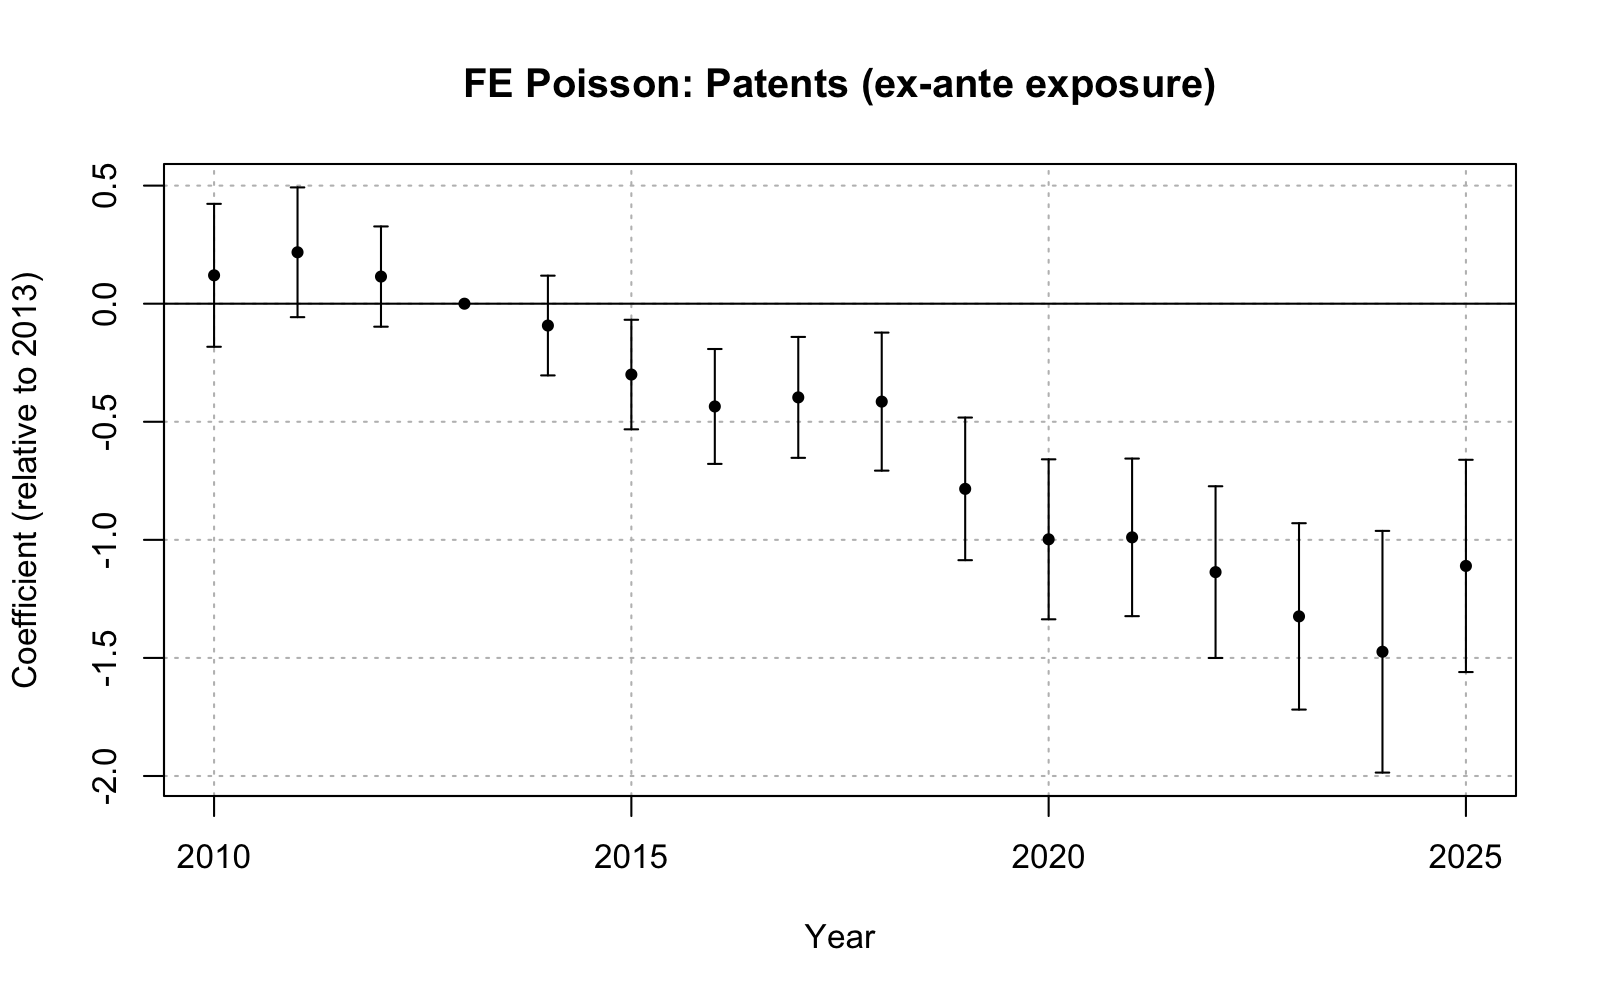
\includegraphics[width=\linewidth]{../output/RQ1/patent_poi_exante.png}
  \caption{FE Poisson event study: patents, ex-ante Medicaid exposure}
  \label{fig:rob_rq1_patent_poi_exante}
\end{figure}

\begin{figure}[!h]
  \centering
  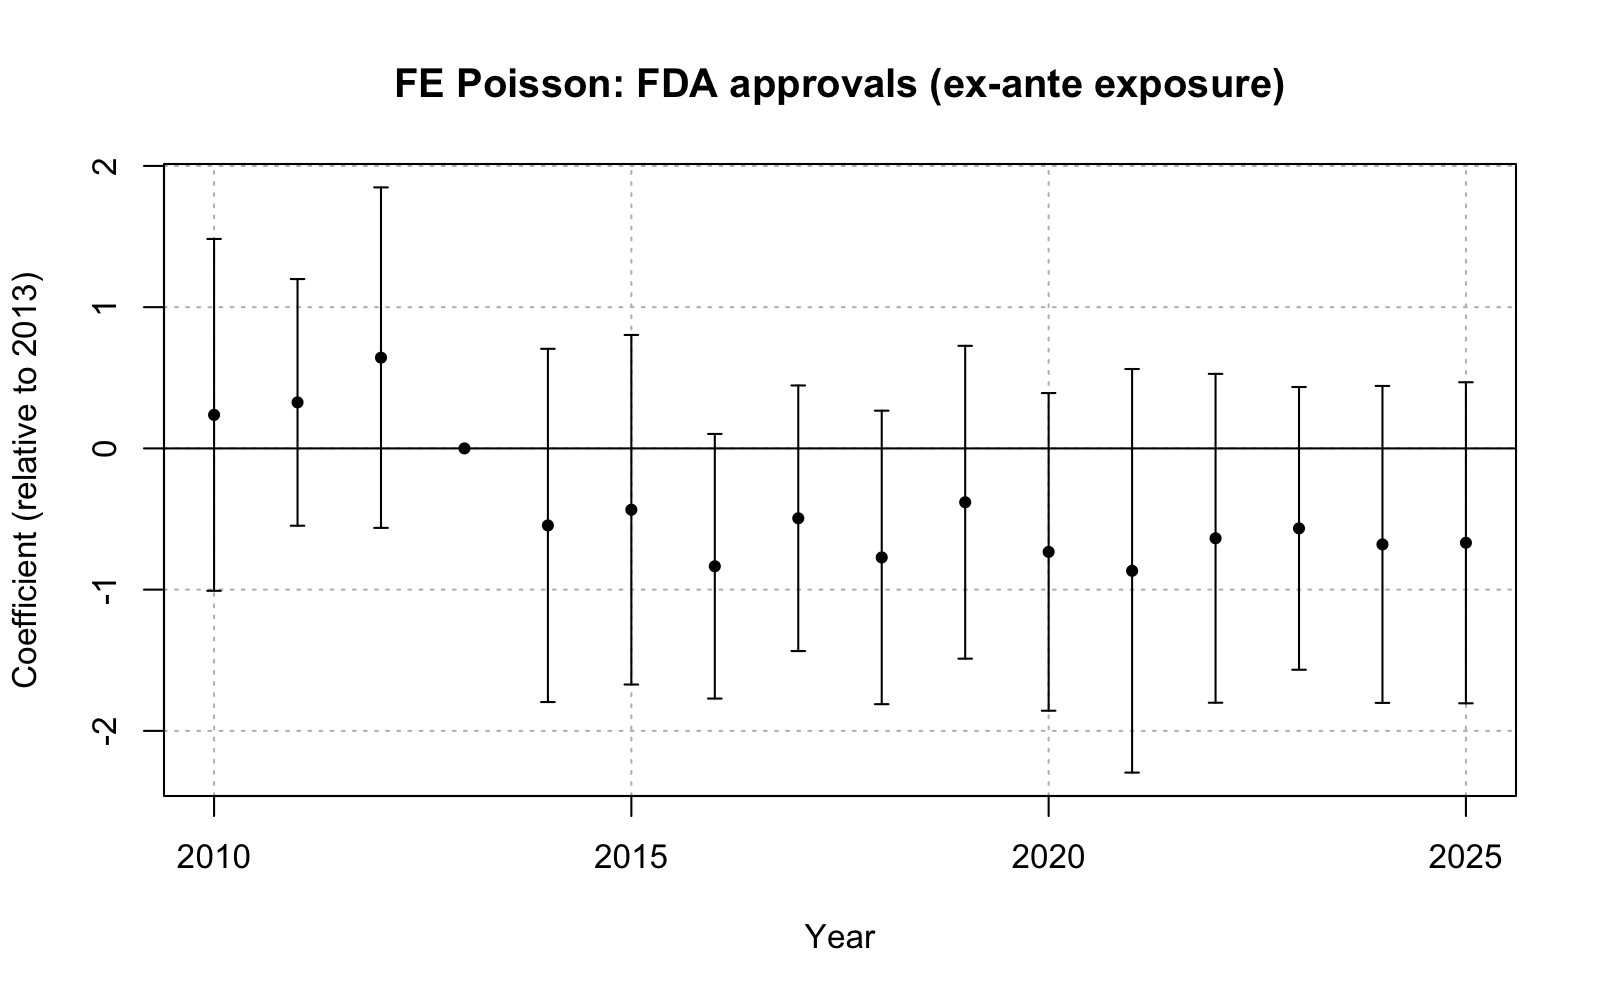
\includegraphics[width=\linewidth]{../output/RQ1/fda_poi_exante.png}
  \caption{FE Poisson event study: FDA approvals, ex-ante Medicaid exposure}
  \label{fig:rob_rq1_fda_poi_exante}
\end{figure}

\clearpage

\subsubsection{Binned Treatment Intensity}

The baseline specification treats exposure to the ACA as a continuous variable. As an alternative test, therapeutic classes are grouped into low, medium and high exposure bins, allowing for separate event-study coefficients to be estimated across different parts of the Medicaid exposure distribution. This relaxes the assumption of linearity in treatment effects imposed by the continuous specification, and examines whether the post-expansion response is concentrated among classes which are greater exposed to the Medicaid reform.

Therapeutic classes are grouped into the three bins based on their ex-ante Medicaid market shares, as reported in Table~\ref{tab:atc_bins}. Nervous system and cardiovascular drugs form the high-exposure bin, as their Medicaid market shares are substantially larger than other class shares. An approximate threshold of 10\% is used to distinguish between the medium and low bin classes, thus anti-infectives and dermatologicals form the medium-exposure bin.


\begingroup
\makeatletter
\renewenvironment{table}[1][tbp]{\@float{table}[#1]}{\end@float}
\makeatother
\input{../output/robustness/binned_treatment/atc_bins.tex}
\endgroup

The low exposure bin is omitted from the regression, so the coefficients for the high and medium bins are estimated relative to the low-exposure bin. The pre-expansion coefficients for both the high and medium-exposure patent bins are small and statistically insignificant, supporting the parallel trends assumption within each group. While the medium-exposure bin largely contain positive insignificant coefficients throughout the post-expansion period with a peak decline of $-0.02$ in 2025, the high-exposure bin exhibit a growing negative trajectory with coefficients reaching $-0.155$ by the same year. This reinforces the finding from RQ3 that the post-expansion patenting decline driven by classes at the upper end of the Medicaid exposure distribution. Importantly, the relative magnitude of the high and medium exposure coefficients is disproportionately larger than their respective Medicaid market shares. On average, exposure of the high bin is approximately $2.5$ times larger than the medium bin, yet the peak patent responses approximately differ by a factor of eight. This suggests that the relationship between Medicaid exposure and patenting may be convex, with the response intensifying at greater levels of exposure as opposed to scaling proportionally.

FDA approval estimates are statistically insignificant for both the high and medium-exposure bins throughout the sample period, and the pre-expansion coefficients are close to zero in both bins, supporting the parallel trends assumption. The absence of significant post-expansion effects for FDA approvals is consistent with the baseline findings and reinforces the interpretation that the innovation response has not yet propagated to the downstream approval stage. Unlike the patent results, the estimates from the FDA binned specification provide no evidence of a non-linear treatment effects across the Medicaid market share distribution, but this is driven by the absence of a detectable effect within each of the exposure bins rather than providing support for a linear relationship.

\clearpage

\begin{figure}[!h]
  \centering
  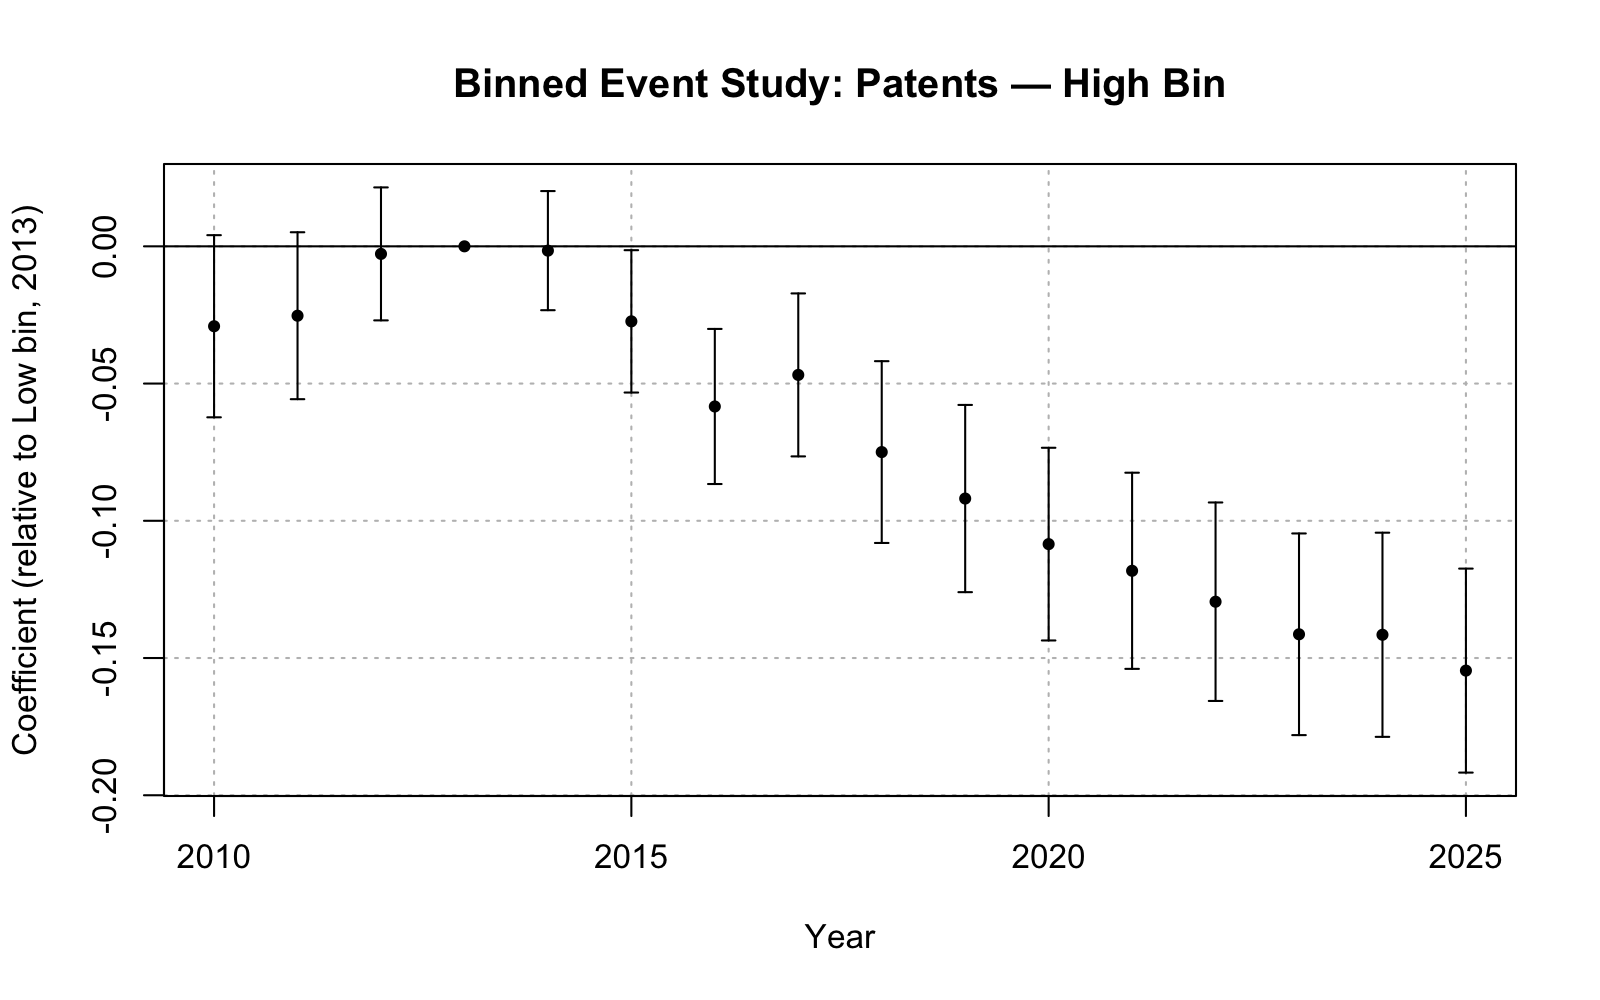
\includegraphics[width=\linewidth]{../output/robustness/binned_treatment/binned_patent_high_es.png}
  \caption{Binned event study: patents, high-exposure bin (N, C)}
  \label{fig:rob_binned_patent_high}
\end{figure}

\begin{figure}[!h]
  \centering
  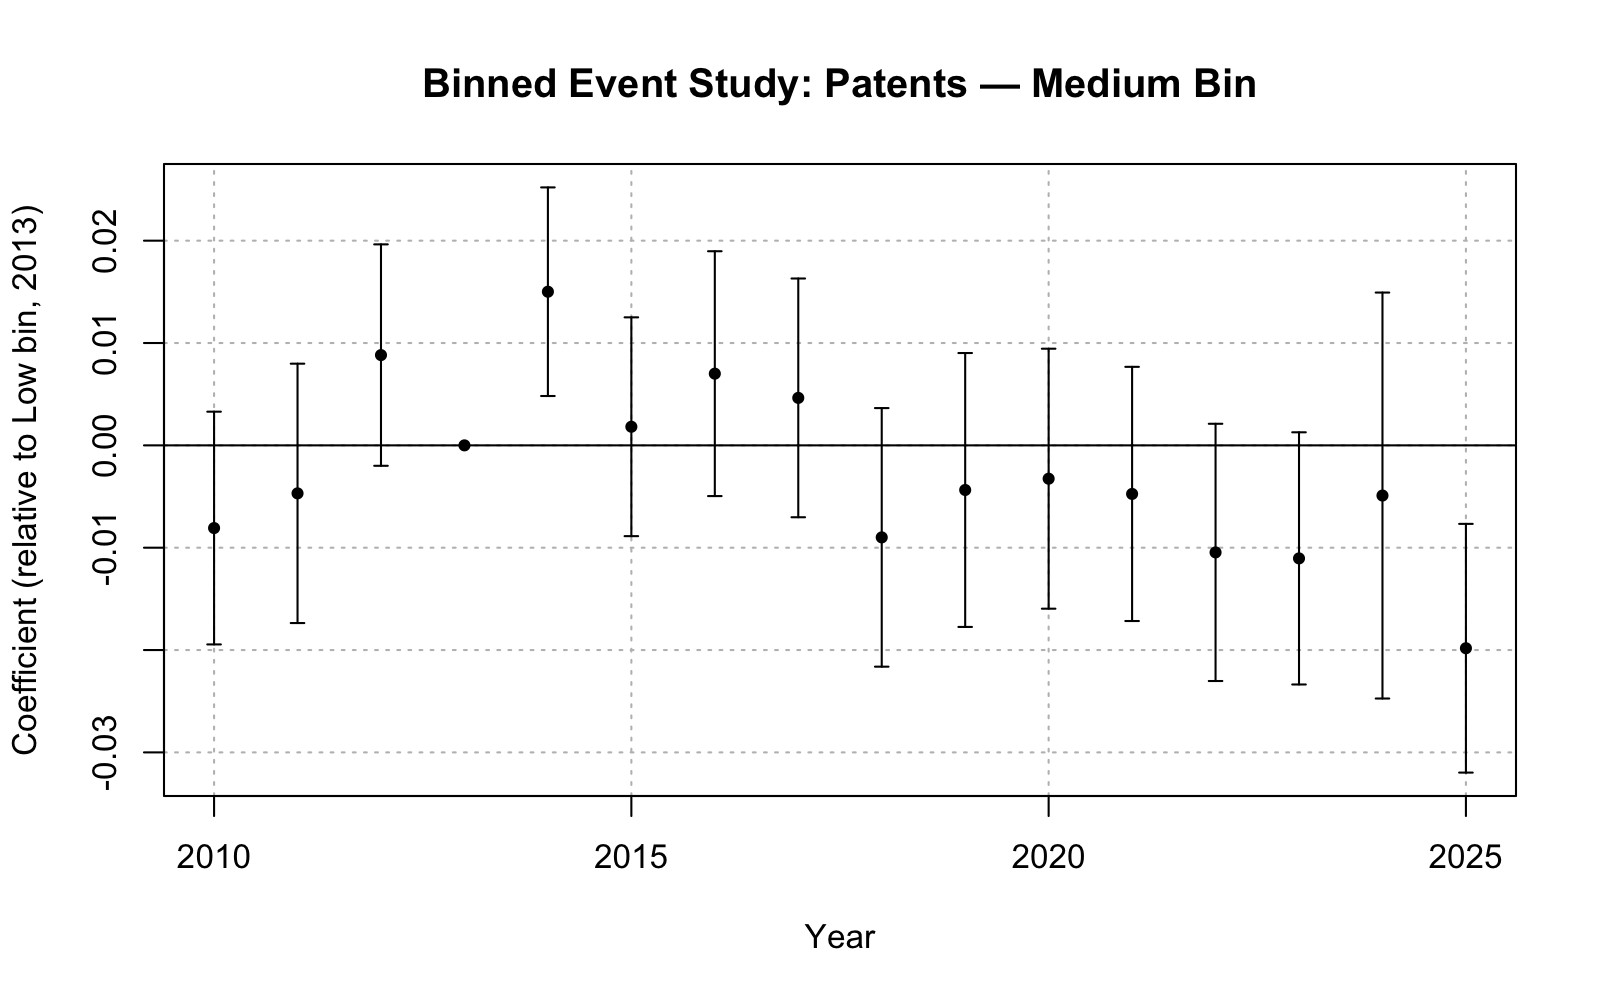
\includegraphics[width=\linewidth]{../output/robustness/binned_treatment/binned_patent_medium_es.png}
  \caption{Binned event study: patents, medium-exposure bin (J, D)}
  \label{fig:rob_binned_patent_medium}
\end{figure}

\clearpage

\begin{figure}[!h]
  \centering
  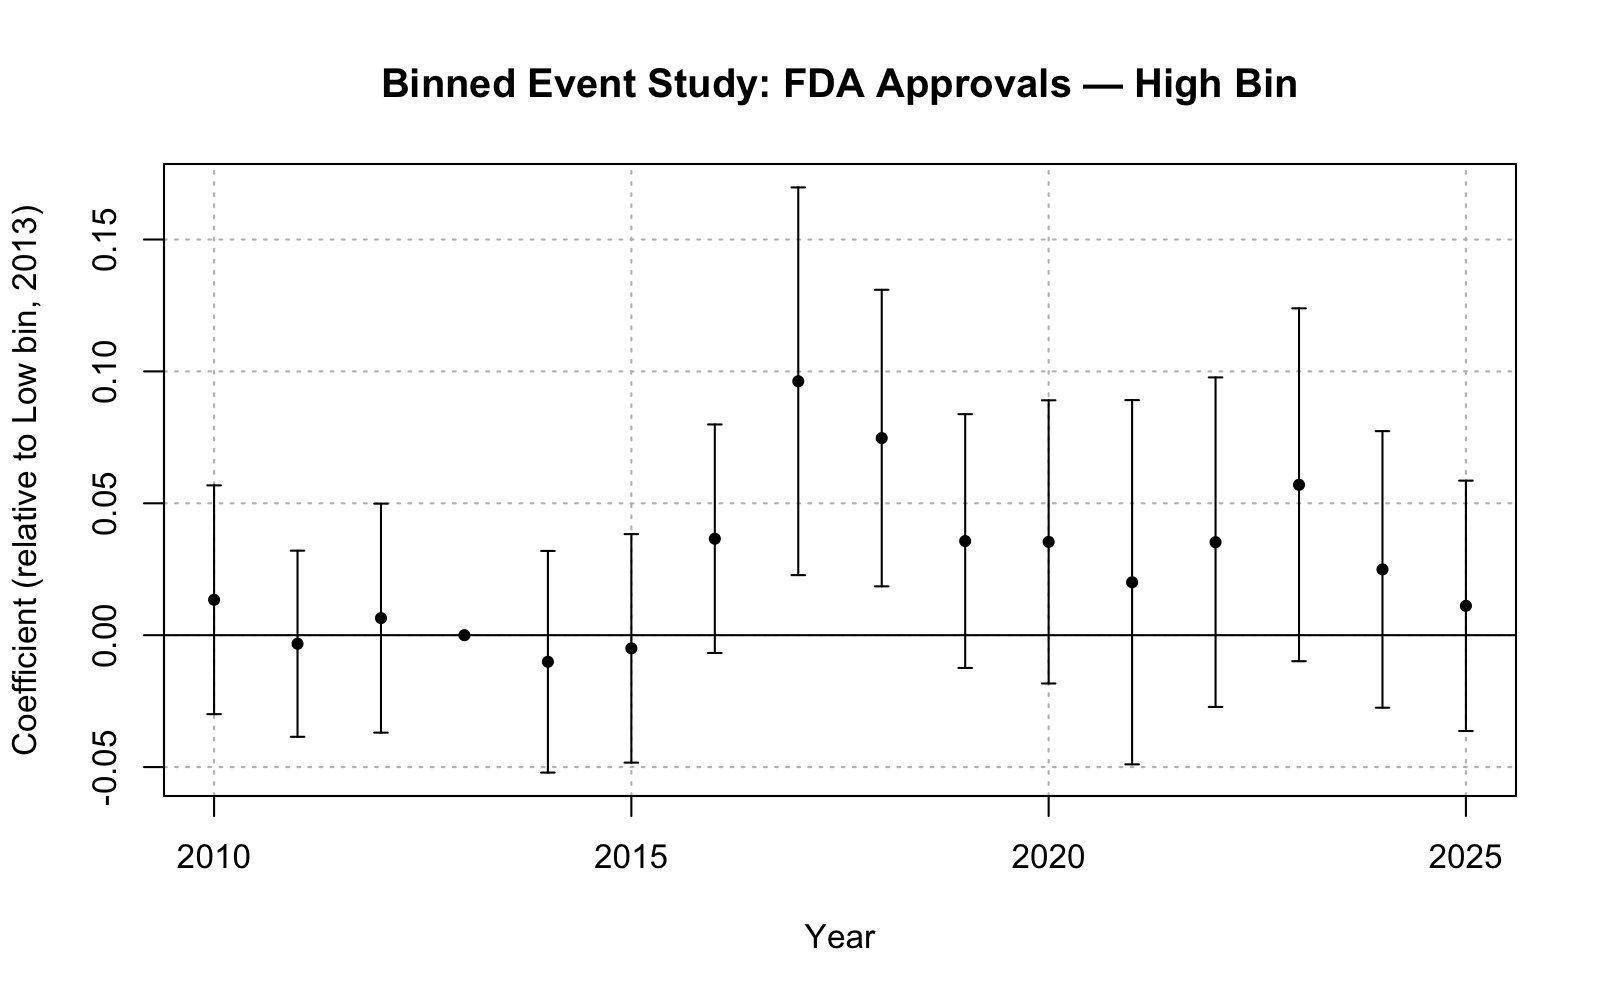
\includegraphics[width=\linewidth]{../output/robustness/binned_treatment/binned_fda_high_es.png}
  \caption{Binned event study: FDA approvals, high-exposure bin (N, C)}
  \label{fig:rob_binned_fda_high}
\end{figure}

\begin{figure}[!h]
  \centering
  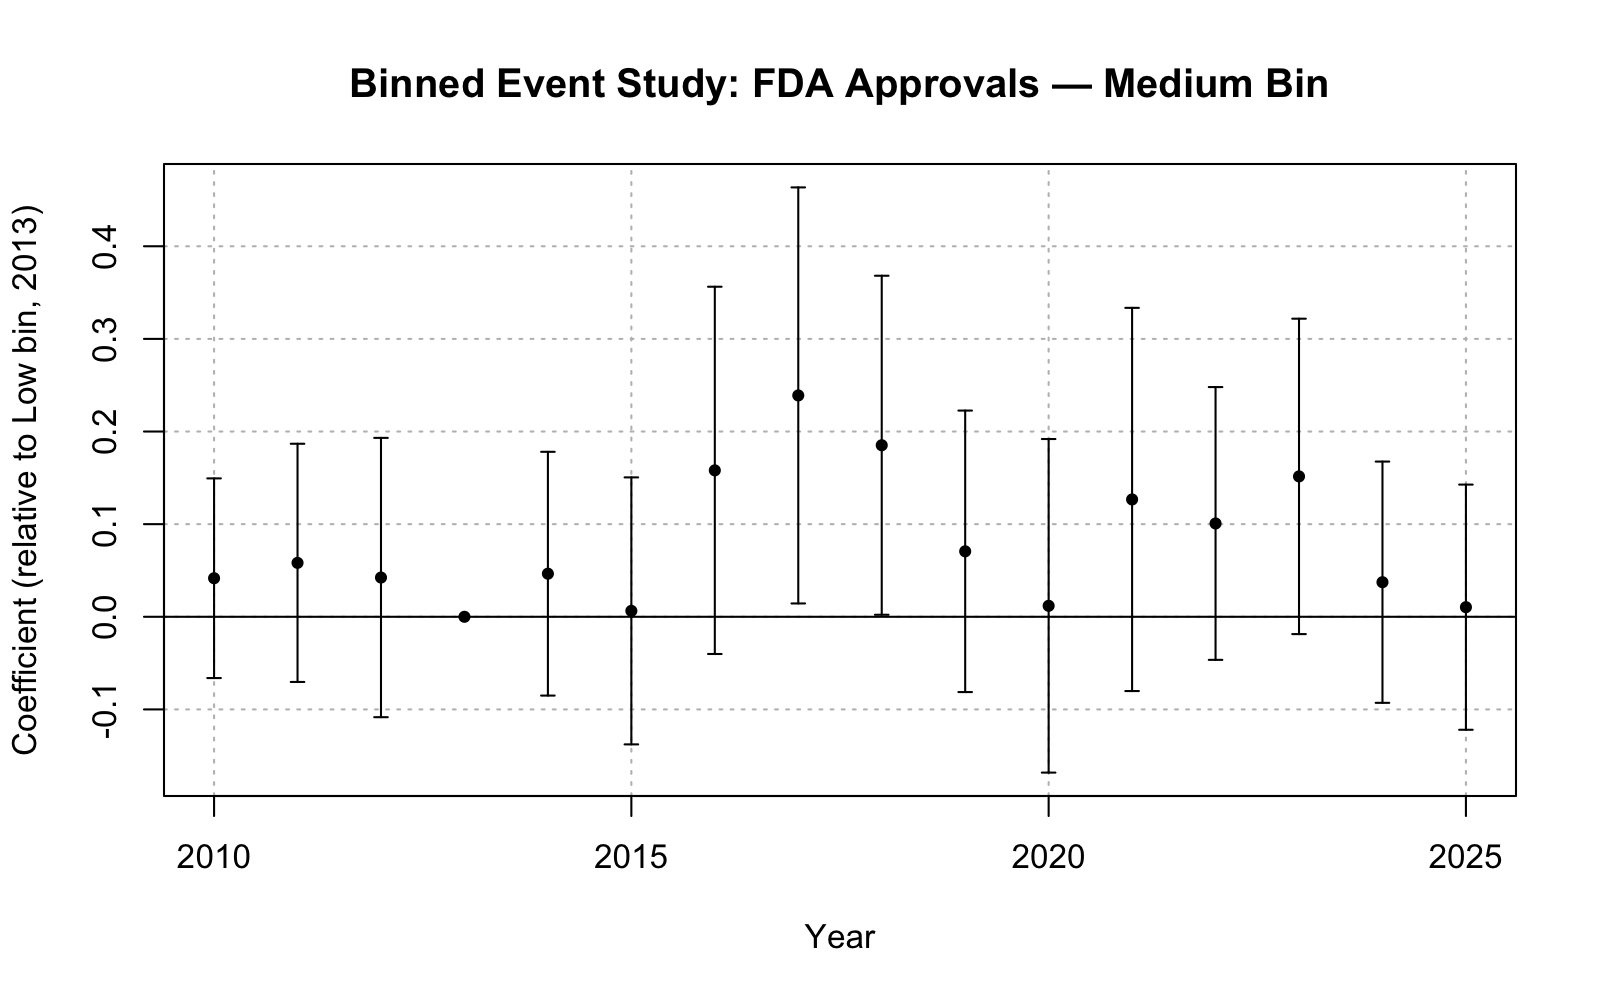
\includegraphics[width=\linewidth]{../output/robustness/binned_treatment/binned_fda_medium_es.png}
  \caption{Binned event study: FDA approvals, medium-exposure bin (J, D)}
  \label{fig:rob_binned_fda_medium}
\end{figure}

\clearpage

\subsubsection{Continuous Difference-in-Differences}

The binned event-study specification allowed for treatment effects to vary across the discrete groups, but the results were contingent on the boundaries specified for each exposure bin. Given this, the continuous difference-in-differences (Continuous DiD) estimator proposed by \citet{NBERw32117} is applied using the \texttt{contdid} R package \citep{contdid2025}. This estimator non-parametrically identifies dose-specific treatment effects at each exposure-level under the parallel trends assumption, thereby avoiding the need to discretise the treatment variable. Conventional TWFE estimators with continuous treatment can be difficult to interpret when treatment effects differ across the distribution of exposure level. The Continuous DiD estimator avoids this by aggregating the dose-specific estimates into event-study coefficients and assesses for pre-trends and post-treatment dynamics. The full set of coefficient estimates is reported in Table~\ref{tab:contdid_es}.

The Continuous DiD estimates for patents are consistent with the baseline results. The pre-expansion coefficients are small and statistically insignificant, supporting the parallel trends assumption. Notably, the coefficients are persistently significant from 2019 onwards, which is four years later than the 2015 onset under the baseline FEOLS model. This implies that the innovation response was not immediate as suggested by the baseline results, instead firms required several years to fully adjust their R\&D decisions in response to the expansion.

The FDA approval estimates under the Continuous DiD model are statistically insignificant throughout the entire period. The pre-period estimates are small and fluctuate around zero, while the post-expansion estimates are mostly positive. The absence of a clear FDA approval response to the Medicaid reform is therefore robust to modelling Medicaid exposure non-parametrically within the Continuous DiD framework.

Taken together, the results from the sensitivity analysis show that the main findings are robust to discretising market shares into exposure bins and using a non-parametric continuous DiD approach. Crucially, the sustained negative patent response remains visible under an estimator developed specifically for continuous-treatment DiD designs, while drug approvals do not appear to have a clear response to the ACA. The Continuous DiD estimates are also consistent with the binned analysis for highly exposed patents, while bins with medium exposure do not display a statistically significant response. This pattern is consistent with the class-level heterogeneity identified in RQ3, where nervous system and cardiovascular drugs were among the classes experiencing the greatest patent reductions.

\clearpage

\begin{figure}[!h]
  \centering
  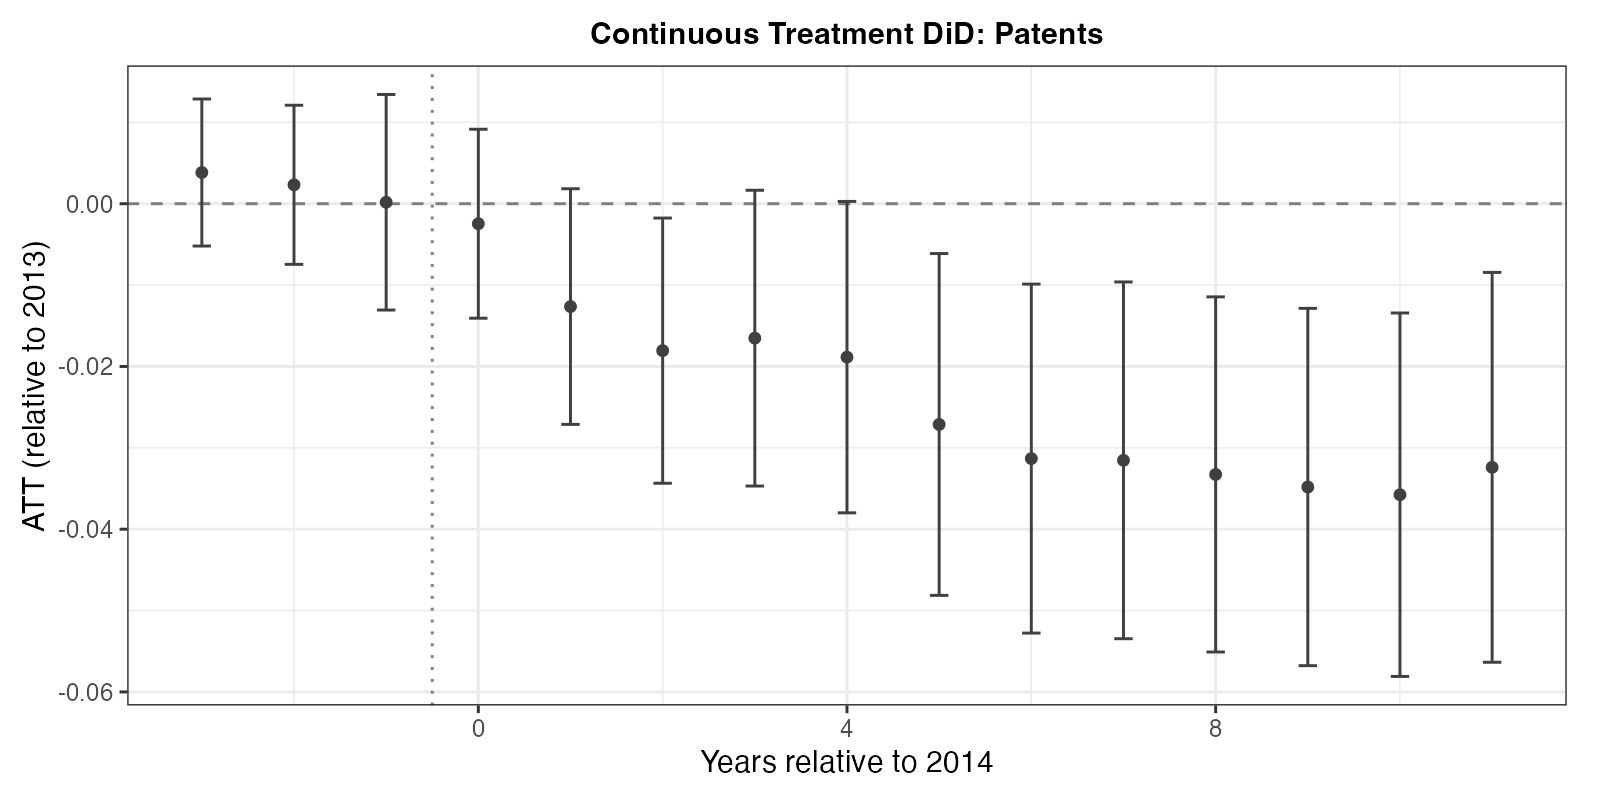
\includegraphics[width=\linewidth]{../output/robustness/contdid/contdid_patent_es.png}
  \caption{Continuous DiD event study: patents}
  \label{fig:rob_contdid_patent}
\end{figure}

\begin{figure}[!h]
  \centering
  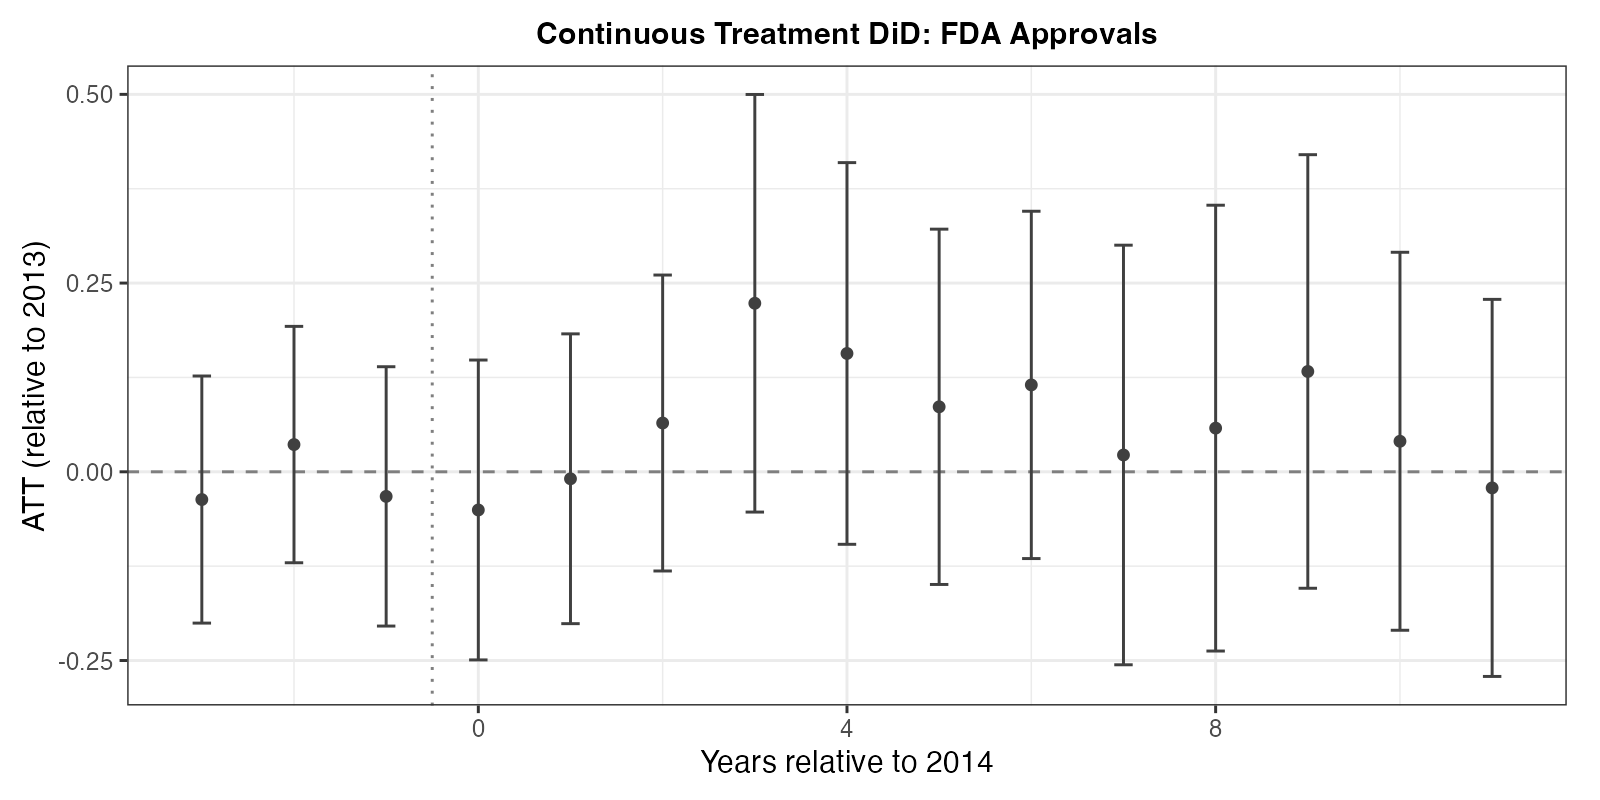
\includegraphics[width=\linewidth]{../output/robustness/contdid/contdid_fda_es.png}
  \caption{Continuous DiD event study: FDA approvals}
  \label{fig:rob_contdid_fda}
\end{figure}

\clearpage

% -----------------------------------------------------------------------
\subsection{RQ2: Medicaid Demand and PDL Exposure}
% -----------------------------------------------------------------------

\subsubsection{Ex-Post Medicaid Exposure}

The second specification jointly estimates the innovation response to Medicaid demand exposure and exposure to the PDL. Like RQ1, an ex-post market share measure is used to determine whether the estimates are sensitive to the construction of the exposure variable.

Once again, the ex-post Medicaid exposure coefficients for patents are nearly identical to the baseline results. The same reductions in Medicaid market share coefficients is observed, with the PDL exposure coefficient path also coinciding with the ex-ante model which saw negative coefficients from 2016 with significance from 2019. The pre-expansion coefficients for both the Medicaid and PDL measures remain small and statistically insignificant, supporting the parallel trends assumption even under the ex-post exposure construction.

The FDA approval coefficients are largely under the ex-post specification are statistically insignificant for both the Medicaid and PDL exposure measures, with isolated incidences of significance in a small number of post-expansion years. This aligns with the baseline finding that the innovation response has not yet reached the final stage of the R\&D pipeline. The agreement between the ex-ante and ex-post results therefore indicates that the decomposition into Medicaid demand and PDL exposure is not sensitive to the construction of exposure to Medicaid.

The FE Poisson, binned treatment, and continuous difference-in-differences estimators are not applied to the RQ2 specification. The joint estimation of two exposure variables under these alternative specifications is computationally demanding, and could not be completed with the device used for this study. Given this constraint, the alternative estimators are only used for the RQ1 specification where they are most informative for the aggregate response to the policy.

\clearpage

\begin{figure}[!h]
  \centering
  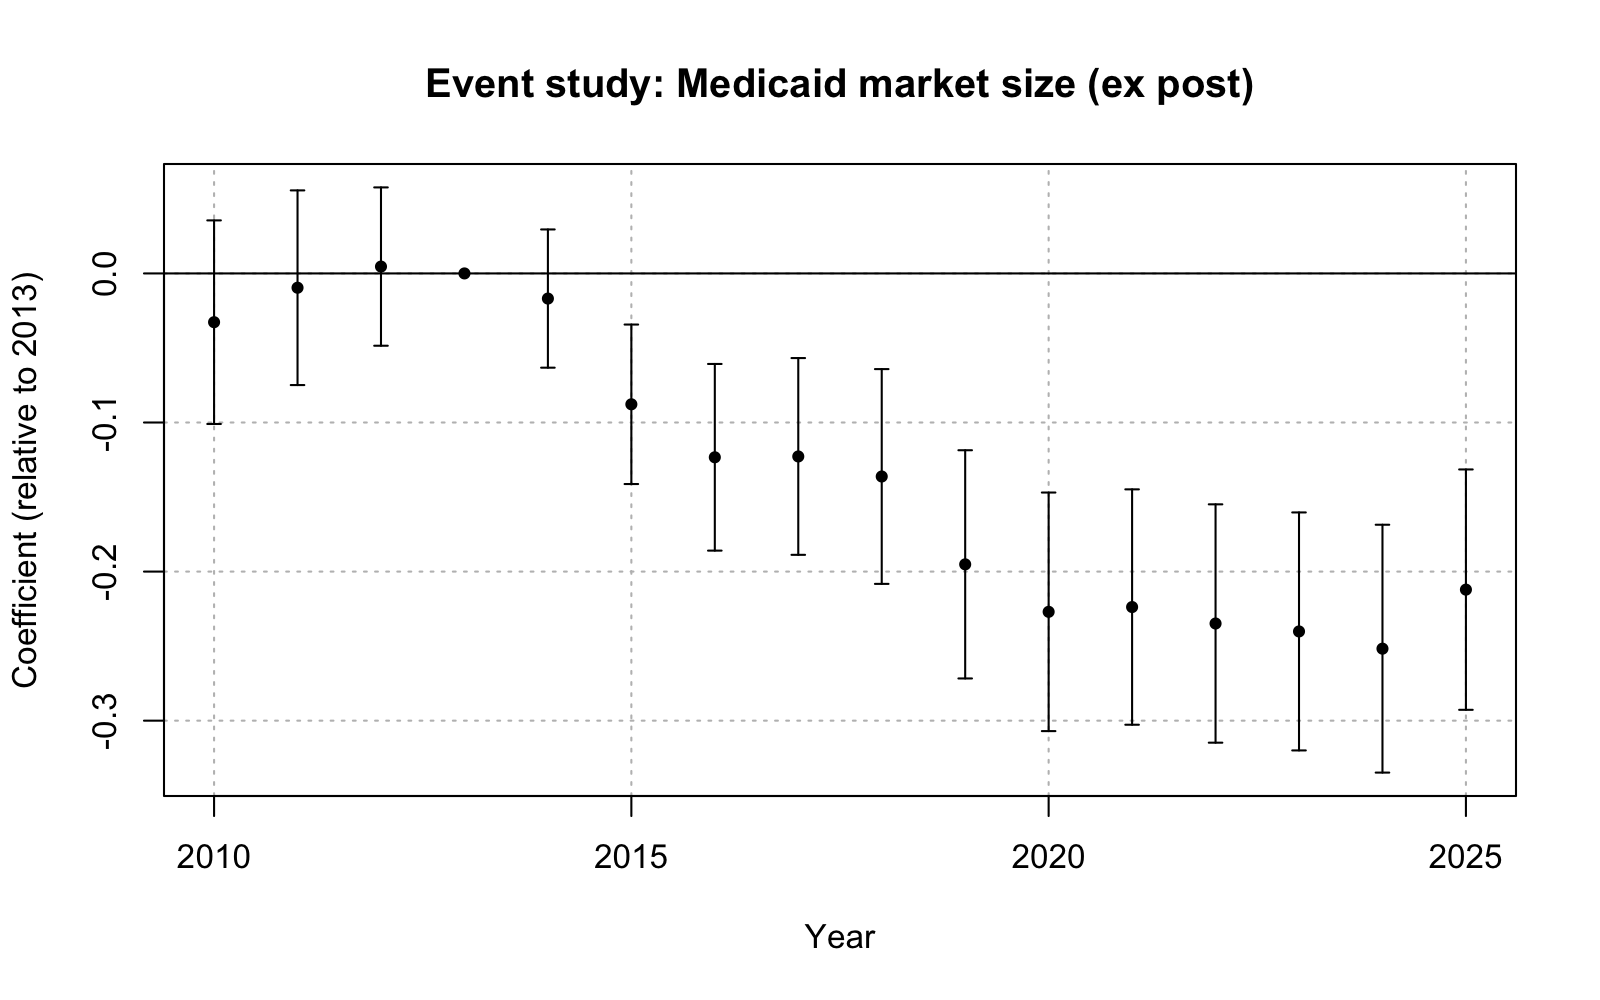
\includegraphics[width=\linewidth]{../output/RQ2/patent_feols_expost_medicaid.png}
  \caption{FEOLS event study: patents, Medicaid exposure (ex-post)}
  \label{fig:rob_rq2_patent_expost_medicaid}
\end{figure}

\begin{figure}[!h]
  \centering
  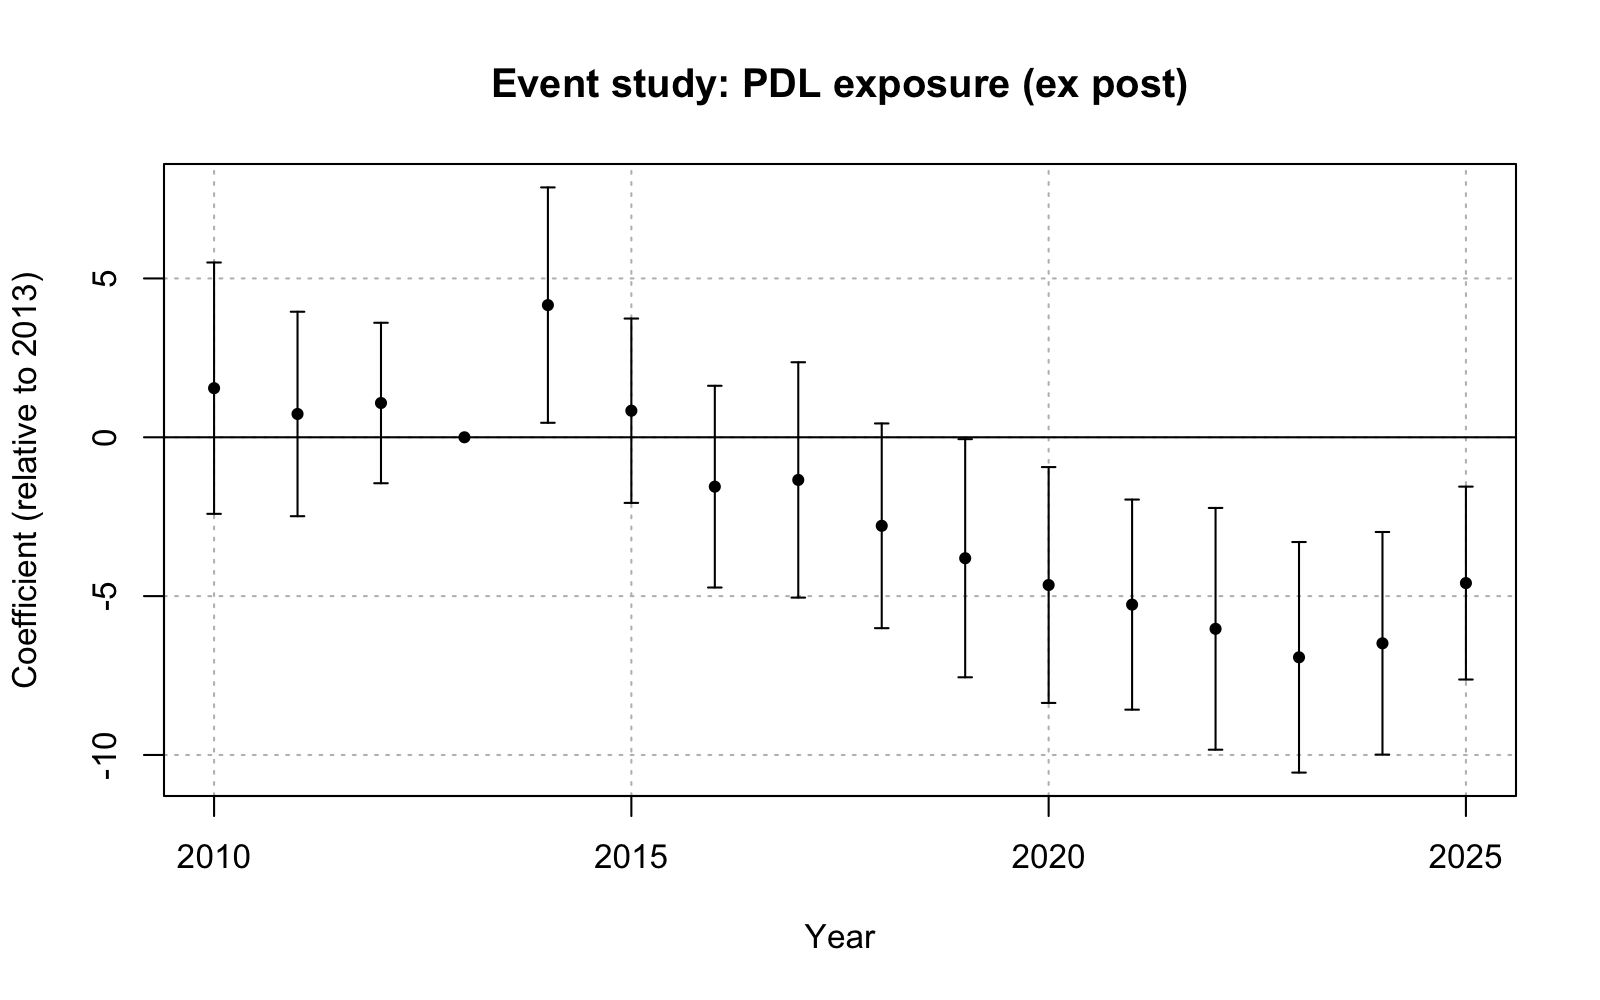
\includegraphics[width=\linewidth]{../output/RQ2/patent_feols_expost_pdl.png}
  \caption{FEOLS event study: patents, PDL exposure (ex-post)}
  \label{fig:rob_rq2_patent_expost_pdl}
\end{figure}

\clearpage

\begin{figure}[!h]
  \centering
  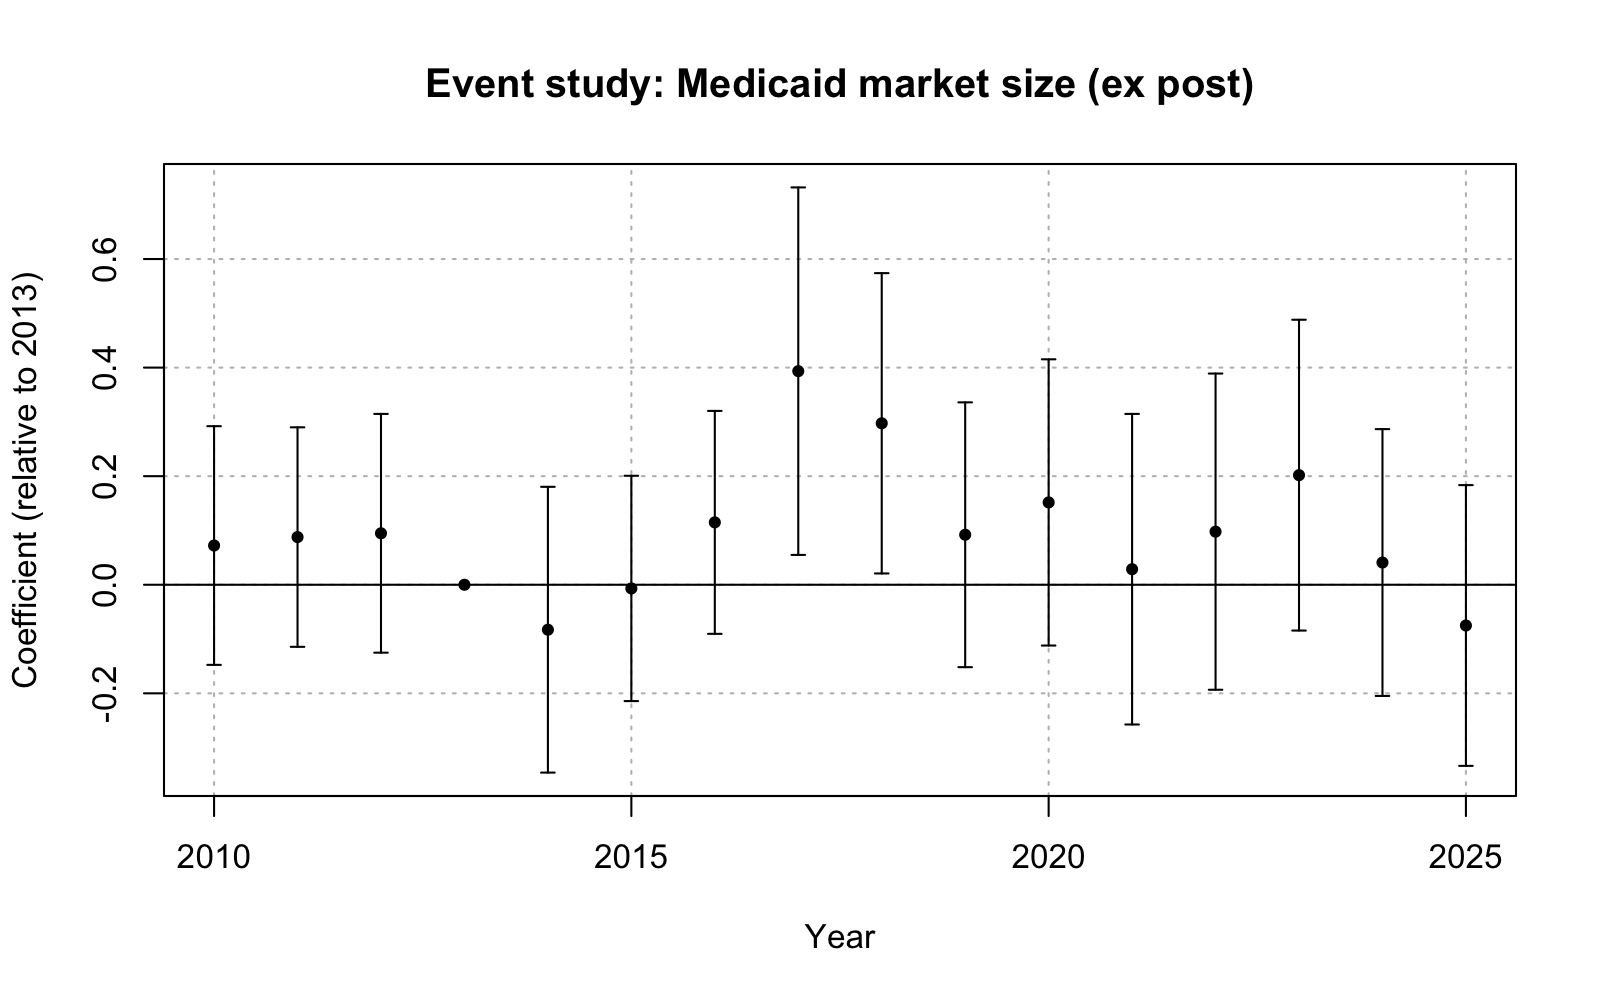
\includegraphics[width=\linewidth]{../output/RQ2/fda_feols_expost_medicaid.png}
  \caption{FEOLS event study: FDA approvals, Medicaid exposure (ex-post)}
  \label{fig:rob_rq2_fda_expost_medicaid}
\end{figure}

\begin{figure}[!h]
  \centering
  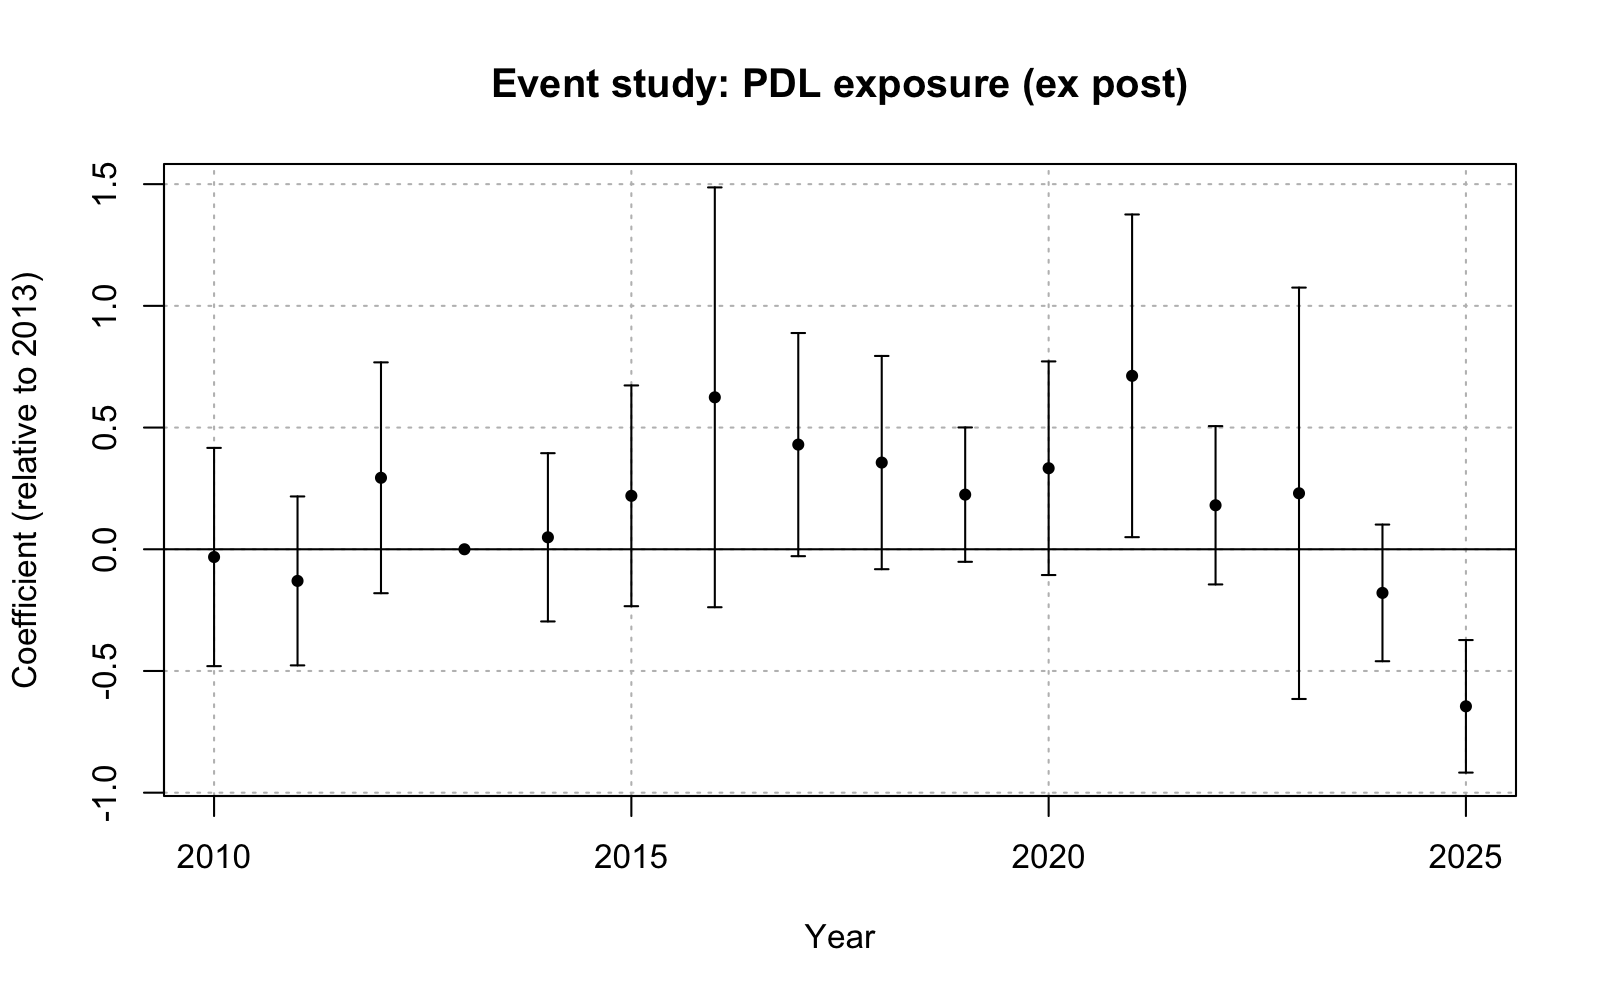
\includegraphics[width=\linewidth]{../output/RQ2/fda_feols_expost_pdl.png}
  \caption{FEOLS event study: FDA approvals, PDL exposure (ex-post)}
  \label{fig:rob_rq2_fda_expost_pdl}
\end{figure}

\clearpage

% -----------------------------------------------------------------------
\subsection{RQ3: Therapeutic-Class Heterogeneity}
% -----------------------------------------------------------------------

\subsubsection{Ex-Post Medicaid Exposure}

The RQ3 specification allows for heterogeneity in innovation behaviour to vary at ATC Level 1 therapeutic class. The ex-post exposure measure of Medicaid exposure is used as a robustness check.

\begin{center}
\begingroup\footnotesize
\input{../output/RQ3/feols_expost_models.tex}
\endgroup
\end{center}


The ex-post estimates are broadly consistent with the ex-ante baseline. Therapeutic classes that exhibited significant negative patent responses under ex-ante exposure, continue to display significant negative coefficients under the ex-post measure. Additionally, positive patent responses are still observed for therapeutic classes relating to blood related drugs, hormonal preparations, and sensory organs. Simiarly, the FDA approval coefficients are aligned with their ex-ante results - significant positive responses for alimentary tract and dermatologicals, and no class are recorded to have a significant reduction in approvals. The results aligning between the two exposure measures indicates that the baseline class-level heterogeneity in innovation response is not driven by the choice of exposure measure.

\subsubsection{Parallel Trends}

The RQ3 triple-difference specification does not take the form of an event study, as the estimation of class-specific dynamic coefficients would be computationally intensive. Consequently, pre-trends coefficients cannot be estimated directly, so the parallel trends assumption cannot be tested for in the same manner as RQ1 and RQ2. Since ATC class V is the omitted from the regressions, it is the reference group for the DDD models. In this context, this specifically indicates that absent the ACA, the relationship between Medicaid exposure and changes in innovation outcomes would have evolved similarly across therapeutic classes relative to class V. The results from earlier the earlier analyses and the model structure can provide evidence to support the plausibility of this assumption.

First, the RQ1 and RQ2 event studies consistently display small and statistically insignificant pre-expansion coefficients across all specifications, including FEOLS, FE Poisson, binned treatment and the continuous DiD approach. Therefore, therapeutic classes with differing levels of Medicaid exposure followed similar innovation trajectories prior to the ACA expansion. Since the same Medicaid exposure measure and firm-class panels are used for RQ3, the evidence for parallel trends from RQ1 and RQ2 provide support for the key identifying assumption of RQ3.

Third, as discussed in the methodology, a violation of parallel trends would require an additional shock around 2014 that differentially affected innovation within therapeutic classes such that it was correlated with exposure to Medicaid. There are no clear candidates for such a confounding shock.

\clearpage

\bibliographystyle{apalike}
\bibliography{references}

\clearpage
\appendix

% -----------------------------------------------------------------------
\section{Robustness Regression Tables}
% -----------------------------------------------------------------------

\subsection{RQ1: Ex-Post FEOLS}

\begingroup\footnotesize
\input{../output/RQ1/feols_expost_models.tex}
\endgroup

\clearpage

\subsection{RQ1: FE Poisson (Ex-Ante)}

\begingroup\footnotesize
\input{../output/RQ1/fepois_exante_models.tex}
\endgroup

\clearpage

\subsection{RQ1: FE Poisson (Ex-Post)}

\begingroup\footnotesize
\input{../output/RQ1/fepois_expost_models.tex}
\endgroup

\begin{figure}[!h]
  \centering
  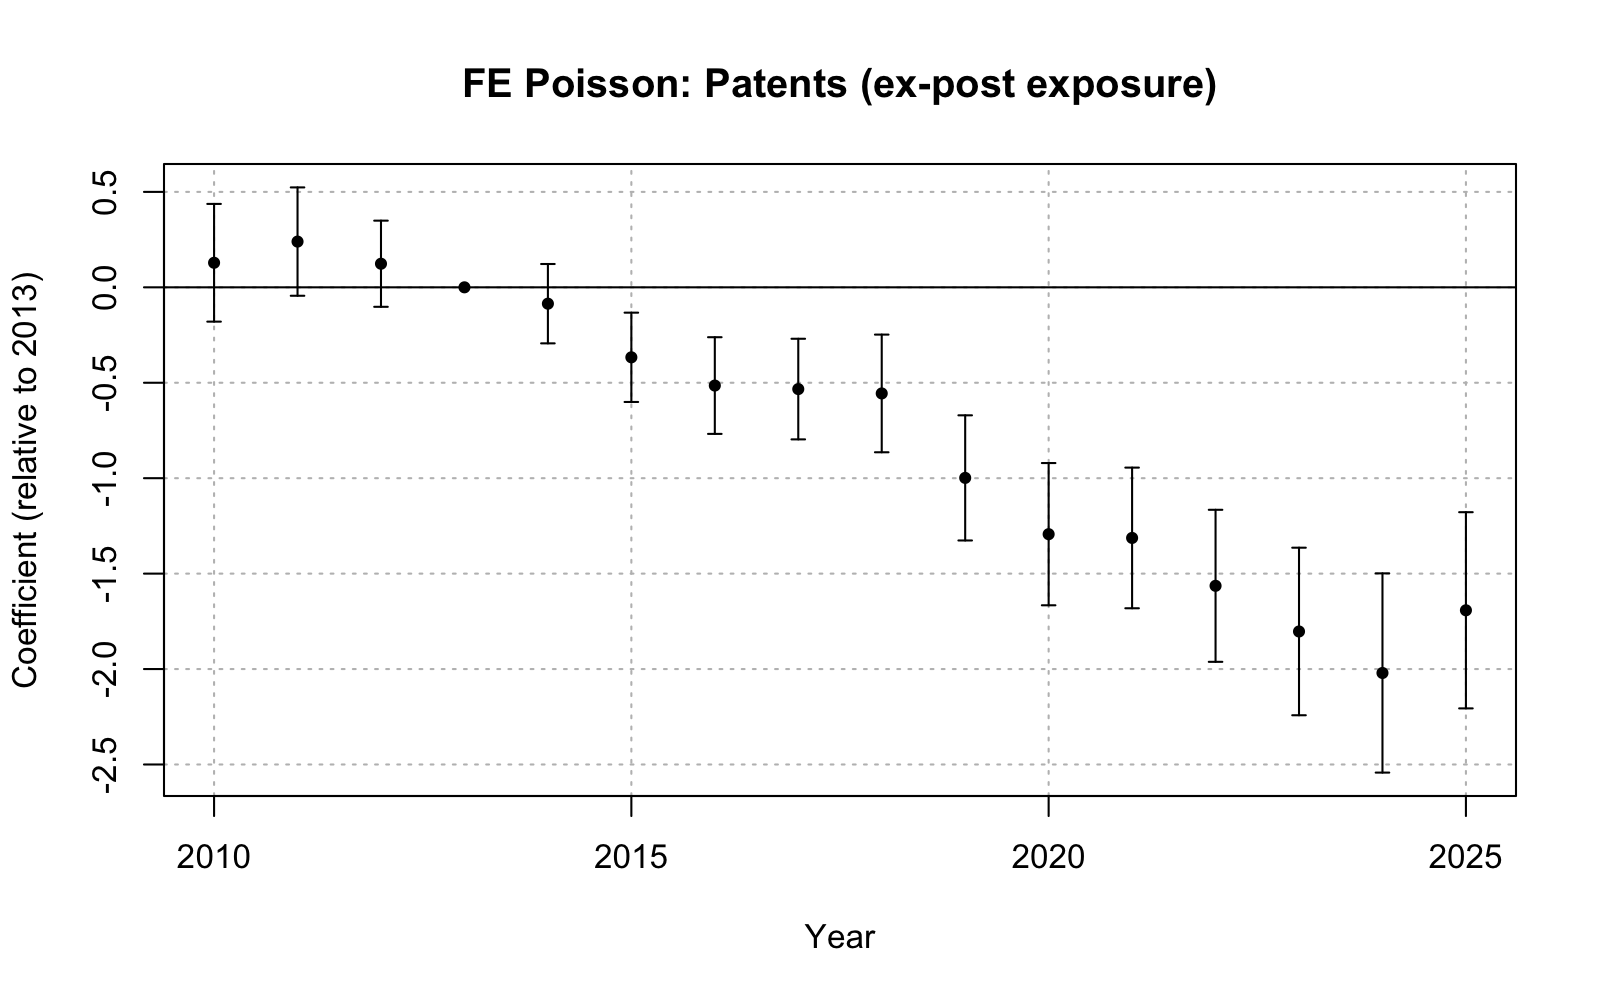
\includegraphics[width=\linewidth]{../output/RQ1/patent_poi_expost.png}
  \caption{FE Poisson event study: patents, ex-post Medicaid exposure}
  \label{fig:rob_rq1_patent_poi_expost}
\end{figure}

\begin{figure}[!h]
  \centering
  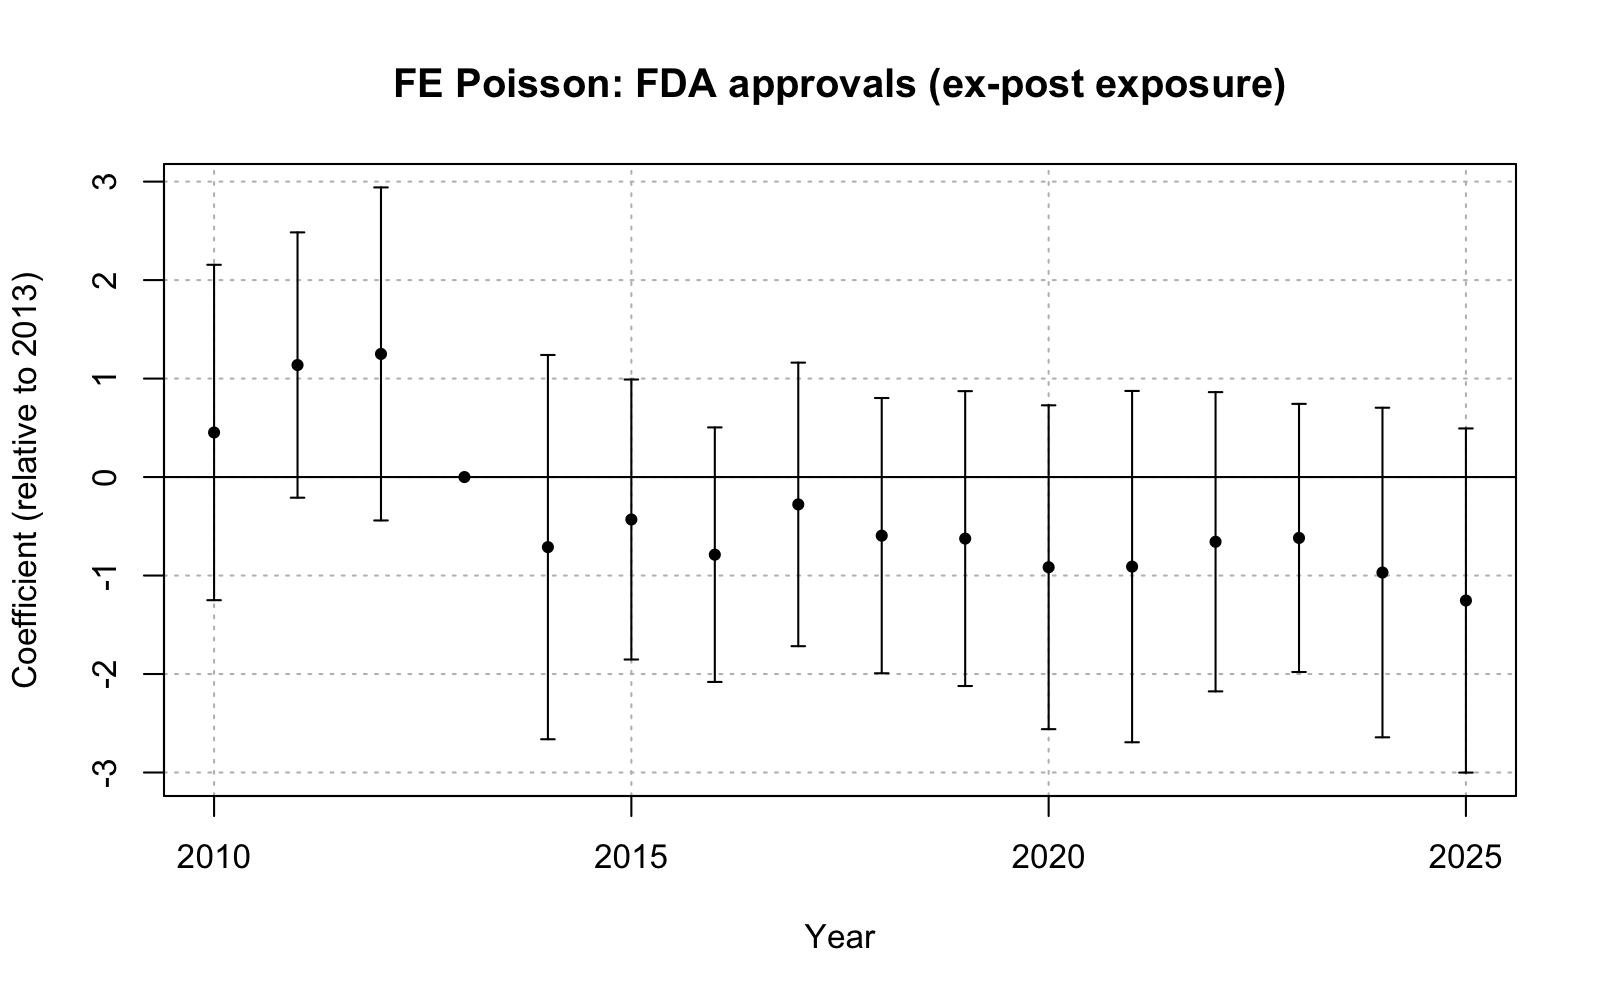
\includegraphics[width=\linewidth]{../output/RQ1/fda_poi_expost.png}
  \caption{FE Poisson event study: FDA approvals, ex-post Medicaid exposure}
  \label{fig:rob_rq1_fda_poi_expost}
\end{figure}

\clearpage

\subsection{RQ1: Binned Treatment}

\begingroup\footnotesize
\input{../output/robustness/binned_treatment/binned_models.tex}
\endgroup

\clearpage

\subsection{RQ1: Continuous Difference-in-Differences}

\begingroup
\makeatletter
\renewenvironment{table}[1][tbp]{\@float{table}[#1]}{\end@float}
\makeatother
\footnotesize
\input{../output/robustness/contdid/contdid_es.tex}
\endgroup

\clearpage

\subsection{RQ2: Ex-Post FEOLS}

\begingroup\footnotesize
\input{../output/RQ2/feols_expost_models.tex}
\endgroup

\end{document}

\input{theoretical_model}
\documentclass[12pt]{article}
\usepackage{geometry}
\geometry{a4paper, portrait, margin=1in}

% --- Math Packages ---
\usepackage{amsmath}
\usepackage{amssymb}
\usepackage{amsfonts}
\usepackage{amsthm}

% --- Graphics & Diagrams ---
\usepackage{graphicx}
\usepackage{tikz}
\usetikzlibrary{shapes, arrows, positioning}

% --- Formatting ---
\usepackage{parskip}
\usepackage[hidelinks]{hyperref}
\usepackage{natbib}
\usepackage{enumitem}
\pagestyle{plain}

% --- Word count (requires compiling with --shell-escape) ---
\newcommand{\wordcount}{%
  \immediate\write18{texcount -sum -1 \jobname.tex 2>/dev/null | python3 -c "import sys; n=sys.stdin.read().strip(); print(f'{int(n):,}') if n.isdigit() else print('?')" > \jobname.wc}%
  \input{\jobname.wc}%
}

\title{MPhil Thesis: Conclusion}
\author{Mohammad-Shah Karim}
\date{May 2026}

\begin{document}

\ifdefined\isdraft\else
\maketitle
\begin{center}
  \small Word count: \wordcount
\end{center}
\fi

\section{Directions for Further Research}

The empirical and theoretical analysis presented in this thesis is subject to several limitations. This section discusses the most important of these and identifies directions in which future work could extend the analysis.

\subsection{Clinical Trial Outcomes}

This thesis chooses to study patenting and drug approvals to capture the innovation stages before and after clinical-trials studied by \citet{NBERw28755}. Clinical trials are an intermediate position between these two outcomes; incorporating clinical-trial data would complete the pipeline comparison, thereby allowing the analysis to trace the innovation response across all three stages. Given the scope of this study, this extension was not feasible within the scope of the present study. \citeauthor{NBERw28755} utilise a proprietary clinical trial data supplied by Cortellis. Constructing a comparable panel from ClinicalTrials.gov would require substantial work. The wording of study titles vary substantially and do not always identify the relevant disease area explicitly. Mapping these records to therapeutic-classes would therefore require imperfect text-based classification. Future work utilising Cortellis could assess whether the negative patenting response identified in this thesis is mirrored at the trial stage.

\subsection{PDL Measurement}

The PDL exposure measure used in this thesis is constructed from the Texas Vendor Drug Program, as this is the only state that has made the full formulary history available in a machine-readable format. While the representativeness analysis indicates that the Texas PDL shares substantial overlap with the New York and Washington, overlap with California is considerably weaker, reflecting differences in state-level formulary structures. This introduces measurement error into the PDL exposure variable, since firms classified as having heavy exposure to the PDL in Texas may be less exposed to it in other states. Consequently, the estimated innovations response to PDL exposure is likely to be attenuated towards zero, and should be interpreted as a plausible lower bound. Further work could construct a multi-state PDL exposure measure using additional formulary records, and average these across states to obtain a more representative measure ofa firm's overall exposure to Medicaid's PDL.

\subsection{Therapeutic Classification}

The analysis aggregates all outcomes to a coarse clinical outcome - ATC Level 1. This can contain drugs with substantially different clinical profiles and competitive environments, so within-class innovation heterogeneity may be masked. This is particularly relevant for the heterogeneity analysis in RQ3, where differences in innovation responses may remain hidden even where the ATC Level 1 estimates appear null or weak. Finer classification such as ATC Levels 2 or 3 may allow the analysis to distinguish between sub-therapeutic areas, but would come at the cost of an increase in panel dimensionality and therefore computational demands. Patents are classified using a CPC-to-ATC crosswalk, and extending to more granular ATC levels would require a mapping that may be noisy.

\subsection{Alternative Estimators for the Joint Specification}

The FE Poisson, binned-treatment, and continuous DiD estimators are applied to the RQ1 specification but not the RQ2 specification separating the innovation responses to both Medicaid and PDL exposure. Extending these estimators to the joint specification exceeded the computational power of the device used for this thesis, due to the size of the firm-class panels and the additional interactions required. The RQ2 estimates are instead supported by the ex-ante and ex-post exposure comparison with the use of FEOLS, but were not subject to equivalent estimator-level sensitivity analysis. Future work could therefore use greater computational capacity to assess whether the decomposition of demand and PDL exposure is robust alternative models.

\subsection{The Theoretical Model}

The theoretical model developed is an illustrative simplification designed to formalise how the Medicaid expansion can reduce innovation incentives through the procurement design. The model restricts competition to two firms competing for access within each therapeutic class, and assumes that the winner of the price stage receives the entire Medicaid market. In reality, several manufacturers compete for PDL authorisation within a therapeutic class, and multiple products may receive preferred placement. The model therefore abstracts from an oligopolistic structure to a duopoly setting in order to isolate the interaction between market size, rebate extraction, and the rent gap rather than the exact number of firms. An $N$-firm extension would allow for the examination of how rebate pressure scales with the number of clinically viable competitors, and whether the Medicaid expansion causes marginal firms to exit Medicaid-relevant therapeutic areas entirely rather than simply reducing innovation effort.

\section{Conclusion}

This thesis has examined whether the ACA Medicaid expansion raised pharmaceutical innovation, and whether the response depended on firms' exposure to Medicaid's procurement institutions. Conventionally, an expansion in expected demand should increase the expected return to R\&D \citep{finkelstein2004static, dubois2015market}. However, the Medicaid setting alters this prediction, as the additional demand is subject to statutory rebates, supplemental rebate negotiations, and drug-list bargaining. To study this question, the analysis constructed novel firm-therapeutic-class panels linking both patent records and FDA drug approvals to Medicaid prescription data, and PDL placement over 2010-2025.

The main empirical finding is that therapeutic classes with greater exposure to Medicaid experienced a persistent decline in patenting following the 2014 reform, while FDA approvals had an inconclusive response. The divergence between patents and FDA approvals is consistent with the changes in patenting behaviour appearing earlier in the R\&D pipeline, with insufficient time passing for changes in drug development to reach the approval stage. This interpretation explains the null effect documented in clinical trials by \citet{NBERw28755}.

A decomposition of innovation behaviour by demand and PDL exposure revealed that firms with greater exposure to Medicaid's PDL experienced additional declines in patenting beyond the demand channel. The PDL counterfactual analysis provides further suggestive support for this where firms securing The aggregate decline in patenting is not uniform across the pharmaceutical industry, with the declines being concentrated in classes with higher exposure to Medicaid and greater levels of drug substitutability. However, classes with lower drug substitutability instead saw innovation responses consistent with the standard market-size prediction, with a rise in patent applications. The PDL counterfactual adds further to this nuanced mechanism, where firms passing only one stage of the PDL selection process experience the largest declines in patenting, while firms securing full preferred placement exhibited declines, albeit smaller ones.

The theoretical model formalises this procurement-based interpretation. Since rebate extraction strengthened with the Medicaid market expansion, additional demand can lower expected returns to R\&D. This effect is likelier to hold for more clinically substitutable drugs, where Medicaid's bargaining position for deeper rebates is stronger. Notably, the model identifies the gap between monopoly and competitive profits as the key object linking pricing pressure to innovation incentives. Policies that shrink this gap therefore reduce equilibrium effort immediately and in the future period through an internal-financing channel.

Taken together, the findings of this thesis suggest that the consequences of public demand expansions on innovation depend on the interaction between institutions governing how firms capture surpluses and market conditions, such as within-therapeutic-class drug substitutability. The findings speak more broadly to reforms that leverage government purchasing power to place downward pressure on drug prices, including debates surrounding Medicare price negotiation under the 2022 Inflation Reduction Act. Crucially, the analysis suggests that the innovation consequences of such reforms should be evaluated on a class-by-class basis, since the same demand shock may encourage R\&D in some therapeutic areas while weakening incentives in others.

\newpage
\bibliographystyle{apalike}
\bibliography{references}

\end{document}


% ===== Bibliography =====
\clearpage
\renewcommand{\refname}{\vspace{-1em}}
\section{References}
\masterbibliographystyle{apalike}
\masterbibliography{references}

% ===== Appendix =====
\clearpage
\section{Appendix}

% --- From data.tex ---

\subsection{Patent Assignee Matching}

%TC:ignore
\makeatletter
\renewenvironment{table}[1][H]{\@float{table}[H]}{\end@float}
\makeatother
\begin{table}[!h]
\centering
\caption{\label{tab:patent_matching_summary}Pre-2014 patent share: matched vs unmatched assignees}
\centering
\begin{tabular*}{\textwidth}{l@{\extracolsep{\fill}}rr}
\toprule
 & Matched & Unmatched \\
\midrule
Pre-2014 patent share & 35.8\% & 34.6\% \\
Post-2014 patent share & 64.2\% & 65.4\% \\
\bottomrule
\end{tabular*}
\end{table}


\begin{table}[!h]
\centering
\caption{\label{tab:patent_matching_atc}ATC1 share of A61P patents: matched vs unmatched}
\centering
\begin{tabular*}{\textwidth}{l@{\extracolsep{\fill}}rr}
\toprule
ATC1 & Matched & Unmatched \\
\midrule
A & 10.1\% & 10.3\% \\
B & 4.0\% & 3.8\% \\
C & 7.9\% & 7.7\% \\
D & 5.7\% & 5.7\% \\
G & 5.1\% & 4.5\% \\
H & 2.2\% & 1.8\% \\
J & 8.4\% & 9.4\% \\
L & 15.6\% & 16.6\% \\
M & 9.3\% & 9.6\% \\
N & 9.7\% & 9.7\% \\
P & 1.2\% & 1.4\% \\
R & 4.8\% & 4.4\% \\
S & 3.9\% & 3.3\% \\
V & 12.0\% & 11.7\% \\
\bottomrule
\end{tabular*}
\end{table}


\renewenvironment{table}[1][]{}{}
%TC:endignore

\subsection{PDL Exposure Distribution}

\begin{figure}[!h]
  \centering
  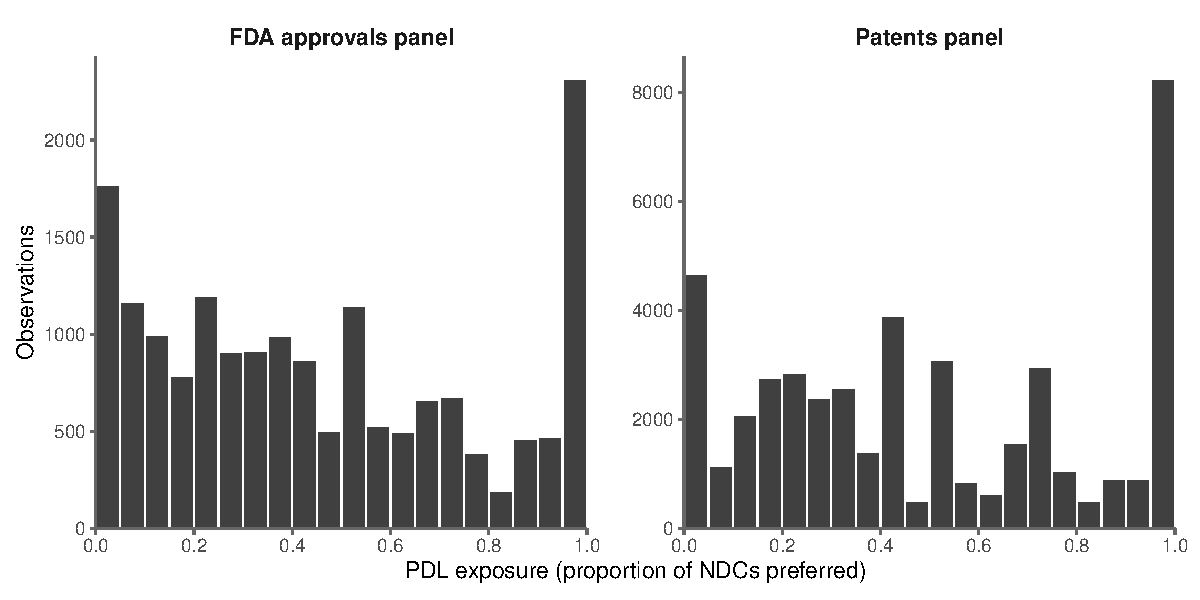
\includegraphics[width=\linewidth]{../output/summary_statistics/pdl_exposure_histogram.pdf}
  \caption{Distribution of PDL exposure in constructed panels}
  \label{fig:pdl_histogram}
\end{figure}

\clearpage

% --- From empirical_results.tex ---

\renewenvironment{table}[1][]{}{}

\subsection{Regression Tables}

\subsubsection{RQ1: Overall Innovation Response}

%TC:ignore
\footnotesize
\begin{table}
\centering
\begin{talltblr}[         %% tabularray outer open
entry=none,label=none,
note{}={* p \num{< 0.05}, ** p \num{< 0.01}, *** p \num{< 0.001}},
]                     %% tabularray outer close
{                     %% tabularray inner open
width=\linewidth,
colspec={Q[]X[]X[]},
column{2,3}={}{halign=c,},
column{1}={}{halign=l,},
hline{32}={1,2,3}{solid, black, 0.05em},
}                     %% tabularray inner close
\toprule
& Patents & FDA Approvals \\ \midrule
2010 × Medicaid Share & \num{-0.041}    & \num{0.215}   \\
                      & (\num{0.038})   & (\num{0.463}) \\
2011 × Medicaid Share & \num{-0.017}    & \num{-0.017}  \\
                      & (\num{0.036})   & (\num{0.381}) \\
2012 × Medicaid Share & \num{0.002}     & \num{0.208}   \\
                      & (\num{0.029})   & (\num{0.412}) \\
2014 × Medicaid Share & \num{-0.022}    & \num{-0.321}  \\
                      & (\num{0.027})   & (\num{0.463}) \\
2015 × Medicaid Share & \num{-0.086}**  & \num{-0.053}  \\
                      & (\num{0.030})   & (\num{0.477}) \\
2016 × Medicaid Share & \num{-0.125}*** & \num{0.414}   \\
                      & (\num{0.034})   & (\num{0.423}) \\
2017 × Medicaid Share & \num{-0.114}**  & \num{1.421}*  \\
                      & (\num{0.036})   & (\num{0.677}) \\
2018 × Medicaid Share & \num{-0.132}*** & \num{0.999}   \\
                      & (\num{0.039})   & (\num{0.550}) \\
2019 × Medicaid Share & \num{-0.189}*** & \num{0.554}   \\
                      & (\num{0.041})   & (\num{0.538}) \\
2020 × Medicaid Share & \num{-0.220}*** & \num{0.732}   \\
                      & (\num{0.043})   & (\num{0.509}) \\
2021 × Medicaid Share & \num{-0.220}*** & \num{0.137}   \\
                      & (\num{0.043})   & (\num{0.632}) \\
2022 × Medicaid Share & \num{-0.233}*** & \num{0.365}   \\
                      & (\num{0.043})   & (\num{0.645}) \\
2023 × Medicaid Share & \num{-0.243}*** & \num{0.846}   \\
                      & (\num{0.044})   & (\num{0.641}) \\
2024 × Medicaid Share & \num{-0.252}*** & \num{0.258}   \\
                      & (\num{0.046})   & (\num{0.523}) \\
2025 × Medicaid Share & \num{-0.228}*** & \num{-0.137}  \\
                      & (\num{0.044})   & (\num{0.510}) \\
Num. obs.             & \num{5281696}   & \num{151200}  \\
R2                    & \num{0.534}     & \num{0.609}   \\
\bottomrule
\end{talltblr}
\end{table}

\captionof{table}{FEOLS event-study estimates: overall innovation response (ex-ante)}
\label{tab:rq1_feols_exante}
\normalsize
%TC:endignore

\clearpage

\subsubsection{RQ2: Medicaid Demand and PDL Exposure}

%TC:ignore
\footnotesize
\begin{table}
\centering
\begin{talltblr}[         %% tabularray outer open
entry=none,label=none,
note{}={* p \num{< 0.05}, ** p \num{< 0.01}, *** p \num{< 0.001}},
]                     %% tabularray outer close
{                     %% tabularray inner open
colspec={Q[]Q[]Q[]Q[]Q[]},
column{2,3,4,5}={}{halign=c,},
column{1}={}{halign=l,},
hline{33}={1,2,3,4,5}{solid, black, 0.05em},
}                     %% tabularray inner close
\toprule
& \SetCell[c=2]{c} Patents && \SetCell[c=2]{c} FDA Approvals & \\
& Medicaid Market Share & PDL Exposure & Medicaid Market Share & PDL Exposure \\ \midrule
2010 & \num{-0.041}    & \num{1.546}     & \num{0.214}   & \num{0.049}   \\
     & (\num{0.038})   & (\num{2.018})   & (\num{0.461}) & (\num{0.807}) \\
2011 & \num{-0.017}    & \num{0.734}     & \num{-0.010}  & \num{-0.243}  \\
     & (\num{0.036})   & (\num{1.642})   & (\num{0.382}) & (\num{0.712}) \\
2012 & \num{0.002}     & \num{1.079}     & \num{0.171}   & \num{1.402}   \\
     & (\num{0.029})   & (\num{1.289})   & (\num{0.406}) & (\num{0.911}) \\
2014 & \num{-0.022}    & \num{4.161}*    & \num{-0.333}  & \num{0.403}   \\
     & (\num{0.026})   & (\num{1.890})   & (\num{0.465}) & (\num{0.647}) \\
2015 & \num{-0.086}**  & \num{0.836}     & \num{-0.088}  & \num{1.163}   \\
     & (\num{0.030})   & (\num{1.480})   & (\num{0.478}) & (\num{0.881}) \\
2016 & \num{-0.126}*** & \num{-1.554}    & \num{0.334}   & \num{2.645}   \\
     & (\num{0.034})   & (\num{1.620})   & (\num{0.426}) & (\num{1.683}) \\
2017 & \num{-0.114}**  & \num{-1.342}    & \num{1.364}*  & \num{1.923}   \\
     & (\num{0.036})   & (\num{1.890})   & (\num{0.680}) & (\num{0.994}) \\
2018 & \num{-0.132}*** & \num{-2.786}    & \num{0.949}   & \num{1.684}   \\
     & (\num{0.039})   & (\num{1.644})   & (\num{0.552}) & (\num{1.021}) \\
2019 & \num{-0.189}*** & \num{-3.806}*   & \num{0.519}   & \num{1.164}*  \\
     & (\num{0.041})   & (\num{1.912})   & (\num{0.539}) & (\num{0.592}) \\
2020 & \num{-0.220}*** & \num{-4.649}*   & \num{0.687}   & \num{1.579}   \\
     & (\num{0.043})   & (\num{1.894})   & (\num{0.514}) & (\num{0.942}) \\
2021 & \num{-0.220}*** & \num{-5.266}**  & \num{0.038}   & \num{3.114}*  \\
     & (\num{0.043})   & (\num{1.687})   & (\num{0.640}) & (\num{1.394}) \\
2022 & \num{-0.233}*** & \num{-6.029}**  & \num{0.333}   & \num{0.994}   \\
     & (\num{0.044})   & (\num{1.941})   & (\num{0.648}) & (\num{0.655}) \\
2023 & \num{-0.243}*** & \num{-6.925}*** & \num{0.809}   & \num{1.185}   \\
     & (\num{0.044})   & (\num{1.851})   & (\num{0.649}) & (\num{1.738}) \\
2024 & \num{-0.252}*** & \num{-6.484}*** & \num{0.272}   & \num{-0.452}  \\
     & (\num{0.046})   & (\num{1.788})   & (\num{0.523}) & (\num{0.590}) \\
2025 & \num{-0.227}*** & \num{-4.588}**  & \num{-0.109}  & \num{-1.118}  \\
     & (\num{0.044})   & (\num{1.549})   & (\num{0.506}) & (\num{0.908}) \\
Num. obs. & \SetCell[c=2]{c} \num{5281696} && \SetCell[c=2]{c} \num{151200} & \\
R2        & \SetCell[c=2]{c} \num{0.535}   && \SetCell[c=2]{c} \num{0.609}  & \\
\bottomrule
\end{talltblr}
\end{table}

\captionof{table}{FEOLS event-study estimates: Medicaid demand and PDL exposure (ex-ante)}
\label{tab:rq2_feols_exante}
\normalsize
%TC:endignore

\clearpage

\subsection{Therapeutic-Class Substitutability}

%TC:ignore
\makeatletter
\renewenvironment{table}[1][H]{\@float{table}[H]}{\end@float}
\makeatother
\begin{table}[!h]
\centering
\caption{\label{tab:class_substitutability}Average annual distinct NDC count by ATC class}
\centering
\begin{tabular}[t]{llr}
\toprule
ATC & Therapeutic class & Mean annual $n_c$\\
\midrule
N & Nervous system & 7351\\
C & Cardiovascular system & 4297\\
A & Alimentary tract and metabolism & 3407\\
J & Anti-infectives for systemic use & 2332\\
D & Dermatologicals & 1771\\
\addlinespace
R & Respiratory system & 1672\\
M & Musculo-skeletal system & 1407\\
B & Blood and blood-forming organs & 1389\\
L & Antineoplastic and immunomodulating & 932\\
G & Genito-urinary and sex hormones & 906\\
\addlinespace
H & Systemic hormonal preparations & 768\\
S & Sensory organs & 579\\
V & Various & 211\\
P & Antiparasitic products & 165\\
\bottomrule
\end{tabular}
\end{table}

\renewenvironment{table}[1][]{}{}
%TC:endignore

\clearpage

% --- From robustness.tex ---

\subsection{Robustness Regression Tables}

\subsubsection{RQ1: Ex-Post FEOLS}

%TC:ignore
\footnotesize
\begin{table}
\centering
\begin{talltblr}[         %% tabularray outer open
entry=none,label=none,
note{}={* p \num{< 0.05}, ** p \num{< 0.01}, *** p \num{< 0.001}},
]                     %% tabularray outer close
{                     %% tabularray inner open
width=\linewidth,
colspec={Q[]X[]X[]},
column{2,3}={}{halign=c,},
column{1}={}{halign=l,},
hline{32}={1,2,3}{solid, black, 0.05em},
}                     %% tabularray inner close
\toprule
& Patents & FDA Approvals \\ \midrule
2010 × Medicaid Share & \num{-0.033}    & \num{0.286}   \\
                      & (\num{0.035})   & (\num{0.450}) \\
2011 × Medicaid Share & \num{-0.010}    & \num{0.336}   \\
                      & (\num{0.033})   & (\num{0.413}) \\
2012 × Medicaid Share & \num{0.004}     & \num{0.414}   \\
                      & (\num{0.027})   & (\num{0.455}) \\
2014 × Medicaid Share & \num{-0.018}    & \num{-0.324}  \\
                      & (\num{0.024})   & (\num{0.533}) \\
2015 × Medicaid Share & \num{-0.088}**  & \num{0.005}   \\
                      & (\num{0.027})   & (\num{0.420}) \\
2016 × Medicaid Share & \num{-0.123}*** & \num{0.550}   \\
                      & (\num{0.032})   & (\num{0.413}) \\
2017 × Medicaid Share & \num{-0.122}*** & \num{1.635}*  \\
                      & (\num{0.034})   & (\num{0.688}) \\
2018 × Medicaid Share & \num{-0.135}*** & \num{1.240}*  \\
                      & (\num{0.037})   & (\num{0.560}) \\
2019 × Medicaid Share & \num{-0.194}*** & \num{0.400}   \\
                      & (\num{0.039})   & (\num{0.497}) \\
2020 × Medicaid Share & \num{-0.225}*** & \num{0.652}   \\
                      & (\num{0.041})   & (\num{0.529}) \\
2021 × Medicaid Share & \num{-0.222}*** & \num{0.218}   \\
                      & (\num{0.040})   & (\num{0.573}) \\
2022 × Medicaid Share & \num{-0.233}*** & \num{0.418}   \\
                      & (\num{0.040})   & (\num{0.590}) \\
2023 × Medicaid Share & \num{-0.238}*** & \num{0.842}   \\
                      & (\num{0.040})   & (\num{0.576}) \\
2024 × Medicaid Share & \num{-0.250}*** & \num{0.137}   \\
                      & (\num{0.042})   & (\num{0.502}) \\
2025 × Medicaid Share & \num{-0.212}*** & \num{-0.380}  \\
                      & (\num{0.041})   & (\num{0.531}) \\
Num. obs.             & \num{5281696}   & \num{151200}  \\
R2                    & \num{0.534}     & \num{0.609}   \\
\bottomrule
\end{talltblr}
\end{table}

\captionof{table}{FEOLS event-study estimates: overall innovation response (ex-post)}
\label{tab:rob_rq1_feols_expost}
\normalsize
%TC:endignore

\begin{figure}[!h]
  \centering
  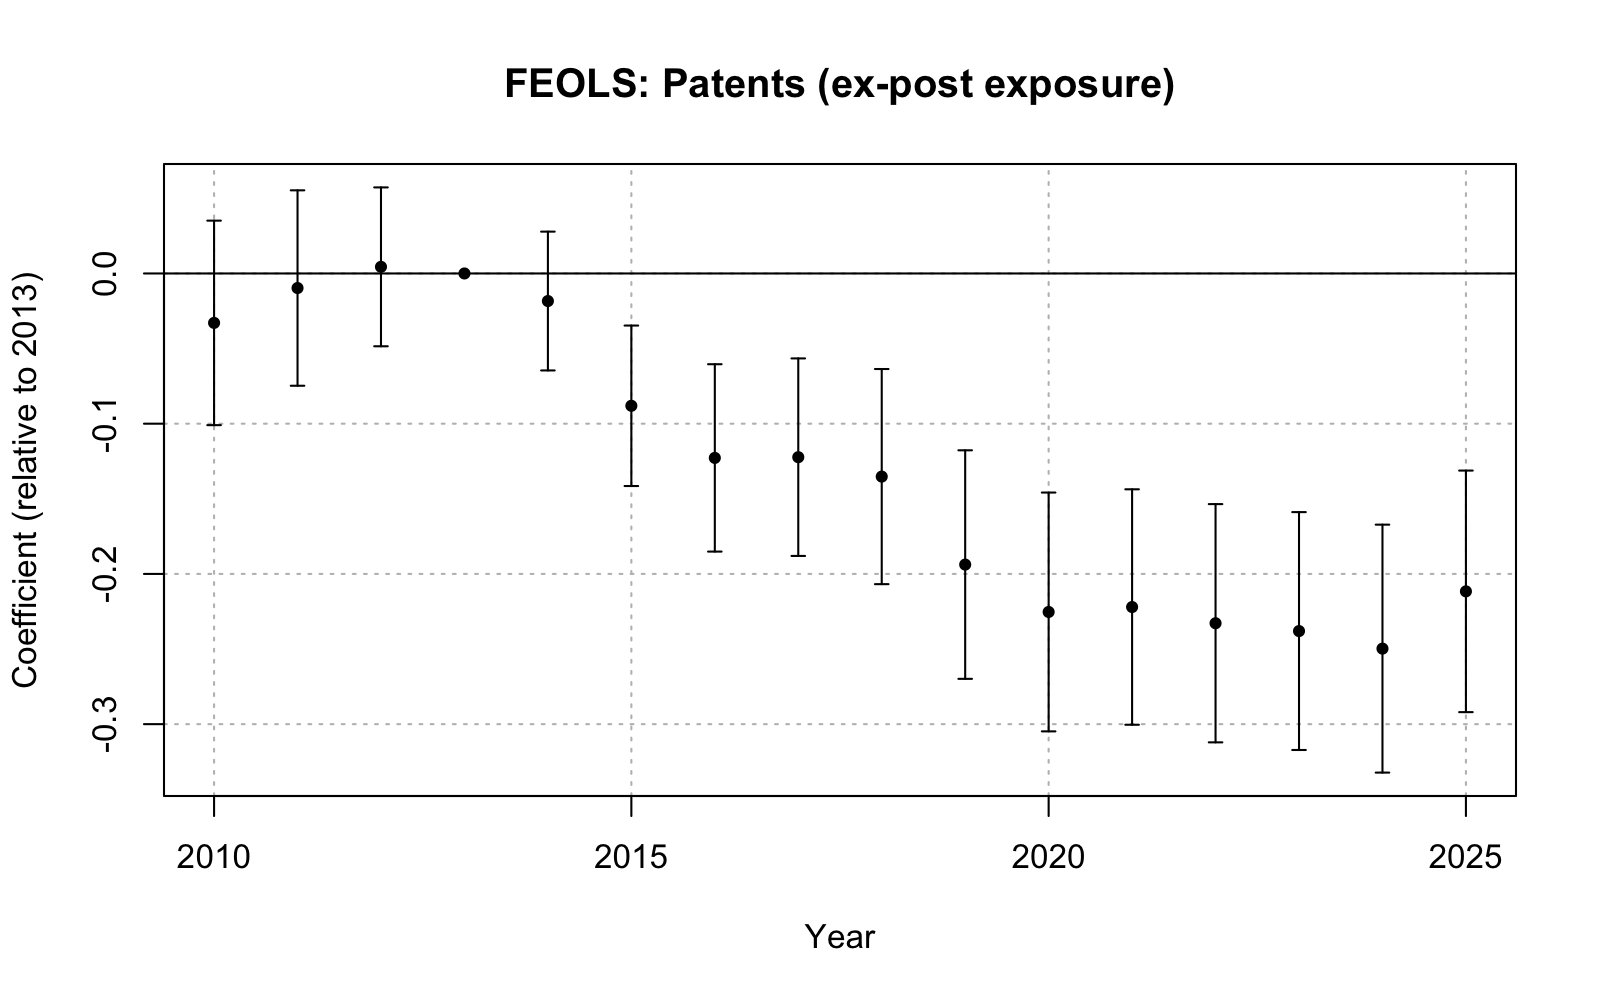
\includegraphics[width=\linewidth]{../output/RQ1/patent_feols_expost.png}
  \caption{FEOLS event study: patents, ex-post Medicaid exposure}
  \label{fig:rob_rq1_patent_feols_expost}
\end{figure}

\begin{figure}[!h]
  \centering
  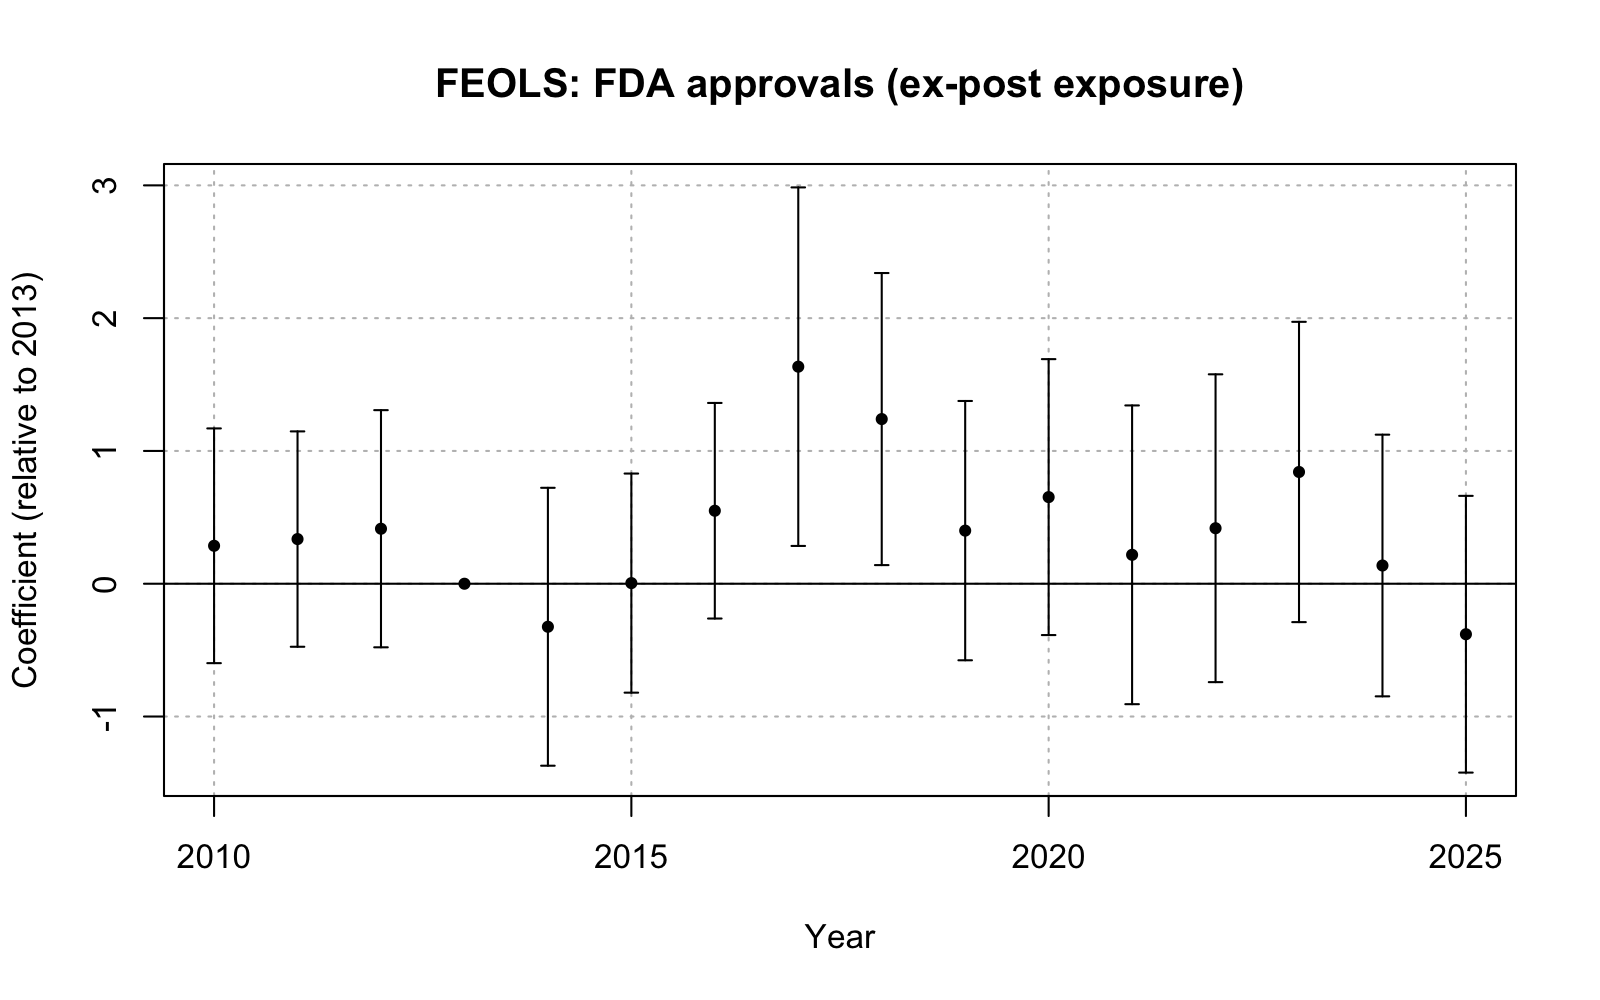
\includegraphics[width=\linewidth]{../output/RQ1/fda_feols_expost.png}
  \caption{FEOLS event study: FDA approvals, ex-post Medicaid exposure}
  \label{fig:rob_rq1_fda_feols_expost}
\end{figure}

\clearpage

\subsubsection{RQ1: Ex-Ante FE Poisson}

%TC:ignore
\footnotesize
\begin{table}
\centering
\begin{talltblr}[         %% tabularray outer open
entry=none,label=none,
note{}={* p \num{< 0.05}, ** p \num{< 0.01}, *** p \num{< 0.001}},
]                     %% tabularray outer close
{                     %% tabularray inner open
width=\linewidth,
colspec={Q[]X[]X[]},
column{2,3}={}{halign=c,},
column{1}={}{halign=l,},
hline{32}={1,2,3}{solid, black, 0.05em},
}                     %% tabularray inner close
\toprule
& Patents & FDA Approvals \\ \midrule
2010 × Medicaid Share & \num{0.120}     & \num{0.237}   \\
                      & (\num{0.154})   & (\num{0.636}) \\
2011 × Medicaid Share & \num{0.218}     & \num{0.326}   \\
                      & (\num{0.140})   & (\num{0.446}) \\
2012 × Medicaid Share & \num{0.115}     & \num{0.643}   \\
                      & (\num{0.108})   & (\num{0.615}) \\
2014 × Medicaid Share & \num{-0.092}    & \num{-0.545}  \\
                      & (\num{0.108})   & (\num{0.638}) \\
2015 × Medicaid Share & \num{-0.300}*   & \num{-0.434}  \\
                      & (\num{0.118})   & (\num{0.632}) \\
2016 × Medicaid Share & \num{-0.435}*** & \num{-0.834}  \\
                      & (\num{0.124})   & (\num{0.478}) \\
2017 × Medicaid Share & \num{-0.397}**  & \num{-0.495}  \\
                      & (\num{0.131})   & (\num{0.480}) \\
2018 × Medicaid Share & \num{-0.415}**  & \num{-0.772}  \\
                      & (\num{0.149})   & (\num{0.530}) \\
2019 × Medicaid Share & \num{-0.784}*** & \num{-0.381}  \\
                      & (\num{0.154})   & (\num{0.565}) \\
2020 × Medicaid Share & \num{-0.998}*** & \num{-0.733}  \\
                      & (\num{0.173})   & (\num{0.574}) \\
2021 × Medicaid Share & \num{-0.989}*** & \num{-0.867}  \\
                      & (\num{0.170})   & (\num{0.729}) \\
2022 × Medicaid Share & \num{-1.137}*** & \num{-0.637}  \\
                      & (\num{0.186})   & (\num{0.594}) \\
2023 × Medicaid Share & \num{-1.324}*** & \num{-0.566}  \\
                      & (\num{0.201})   & (\num{0.511}) \\
2024 × Medicaid Share & \num{-1.474}*** & \num{-0.680}  \\
                      & (\num{0.261})   & (\num{0.573}) \\
2025 × Medicaid Share & \num{-1.110}*** & \num{-0.668}  \\
                      & (\num{0.229})   & (\num{0.580}) \\
Num. obs.             & \num{1300944}   & \num{42176}   \\
\bottomrule
\end{talltblr}
\end{table}

\captionof{table}{FE Poisson event-study estimates: overall innovation response (ex-ante)}
\label{tab:rob_rq1_fepois_exante}
\normalsize
%TC:endignore

\begin{figure}[!h]
  \centering
  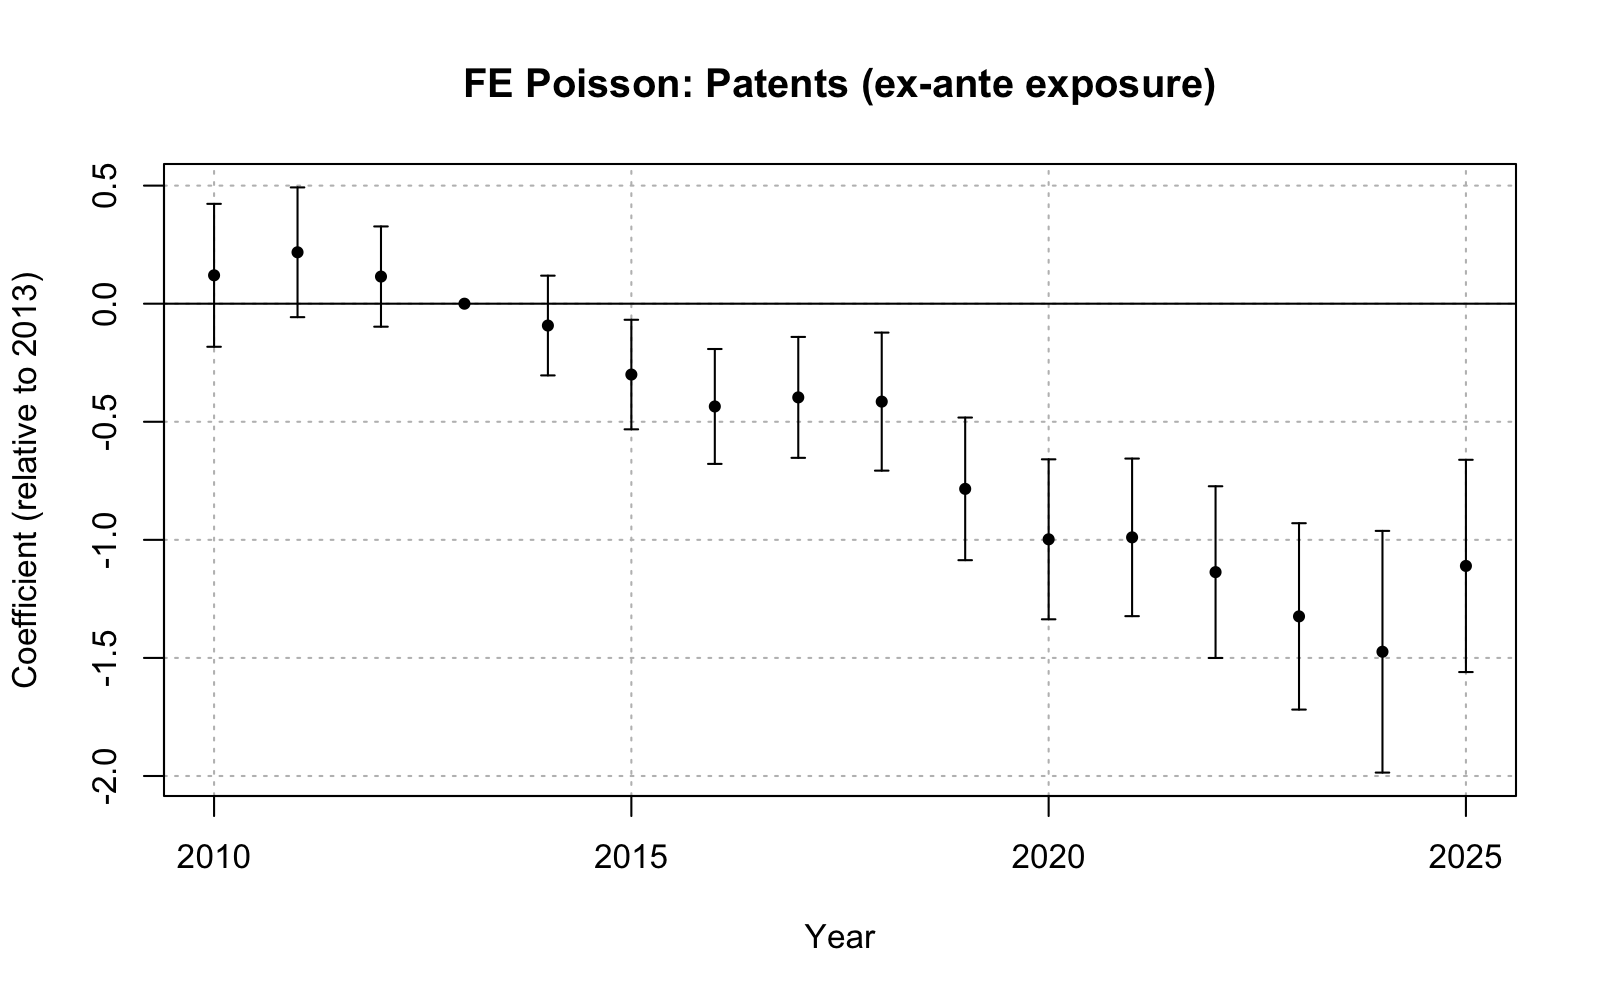
\includegraphics[width=\linewidth]{../output/RQ1/patent_poi_exante.png}
  \caption{FE Poisson event study: patents, ex-ante Medicaid exposure}
  \label{fig:rob_rq1_patent_poi_exante}
\end{figure}

\begin{figure}[!h]
  \centering
  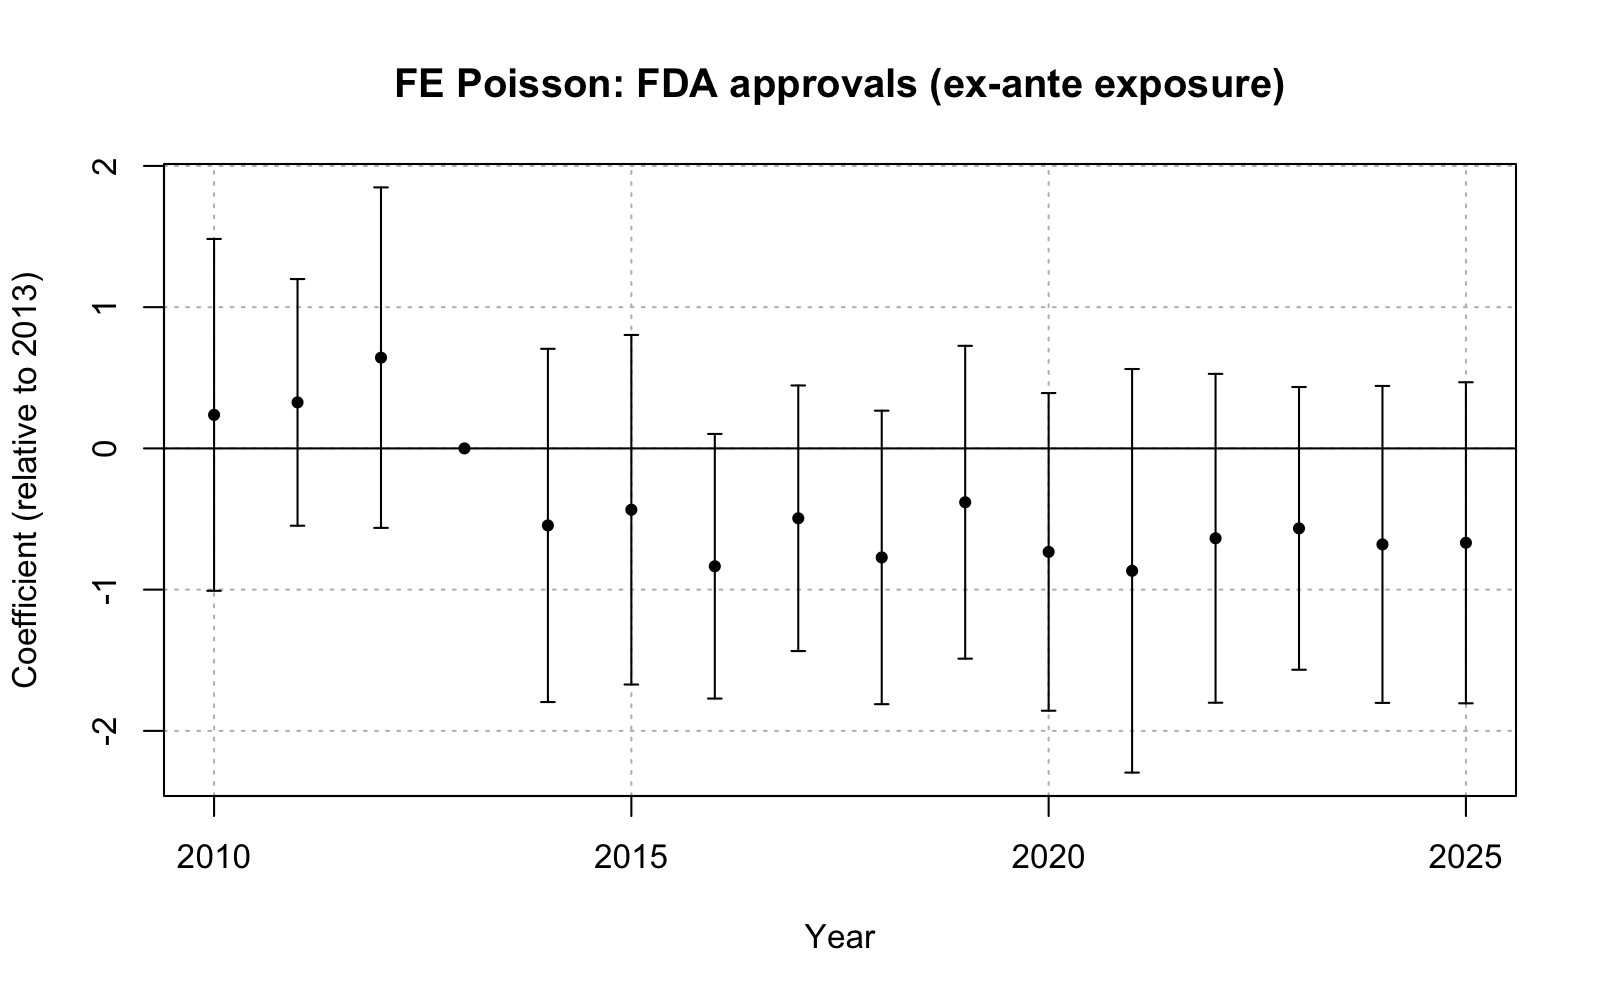
\includegraphics[width=\linewidth]{../output/RQ1/fda_poi_exante.png}
  \caption{FE Poisson event study: FDA approvals, ex-ante Medicaid exposure}
  \label{fig:rob_rq1_fda_poi_exante}
\end{figure}

\clearpage

\subsubsection{RQ1: Ex-Post FE Poisson}

%TC:ignore
\footnotesize
\begin{table}
\centering
\begin{talltblr}[         %% tabularray outer open
entry=none,label=none,
note{}={* p \num{< 0.05}, ** p \num{< 0.01}, *** p \num{< 0.001}},
]                     %% tabularray outer close
{                     %% tabularray inner open
width=\linewidth,
colspec={Q[]X[]X[]},
column{2,3}={}{halign=c,},
column{1}={}{halign=l,},
hline{32}={1,2,3}{solid, black, 0.05em},
}                     %% tabularray inner close
\toprule
& Patents & FDA Approvals \\ \midrule
2010 × Medicaid Share & \num{0.129}     & \num{0.453}   \\
                      & (\num{0.157})   & (\num{0.869}) \\
2011 × Medicaid Share & \num{0.240}     & \num{1.138}   \\
                      & (\num{0.145})   & (\num{0.687}) \\
2012 × Medicaid Share & \num{0.124}     & \num{1.250}   \\
                      & (\num{0.115})   & (\num{0.863}) \\
2014 × Medicaid Share & \num{-0.086}    & \num{-0.711}  \\
                      & (\num{0.106})   & (\num{0.996}) \\
2015 × Medicaid Share & \num{-0.367}**  & \num{-0.431}  \\
                      & (\num{0.119})   & (\num{0.725}) \\
2016 × Medicaid Share & \num{-0.515}*** & \num{-0.788}  \\
                      & (\num{0.129})   & (\num{0.660}) \\
2017 × Medicaid Share & \num{-0.533}*** & \num{-0.278}  \\
                      & (\num{0.134})   & (\num{0.735}) \\
2018 × Medicaid Share & \num{-0.556}*** & \num{-0.595}  \\
                      & (\num{0.157})   & (\num{0.713}) \\
2019 × Medicaid Share & \num{-0.998}*** & \num{-0.625}  \\
                      & (\num{0.167})   & (\num{0.764}) \\
2020 × Medicaid Share & \num{-1.293}*** & \num{-0.916}  \\
                      & (\num{0.190})   & (\num{0.839}) \\
2021 × Medicaid Share & \num{-1.313}*** & \num{-0.909}  \\
                      & (\num{0.188})   & (\num{0.910}) \\
2022 × Medicaid Share & \num{-1.564}*** & \num{-0.657}  \\
                      & (\num{0.203})   & (\num{0.775}) \\
2023 × Medicaid Share & \num{-1.803}*** & \num{-0.618}  \\
                      & (\num{0.224})   & (\num{0.695}) \\
2024 × Medicaid Share & \num{-2.021}*** & \num{-0.969}  \\
                      & (\num{0.266})   & (\num{0.854}) \\
2025 × Medicaid Share & \num{-1.692}*** & \num{-1.254}  \\
                      & (\num{0.262})   & (\num{0.892}) \\
Num. obs.             & \num{1300944}   & \num{42176}   \\
\bottomrule
\end{talltblr}
\end{table}

\captionof{table}{FE Poisson event-study estimates: overall innovation response (ex-post)}
\label{tab:rob_rq1_fepois_expost}
\normalsize
%TC:endignore

\begin{figure}[!h]
  \centering
  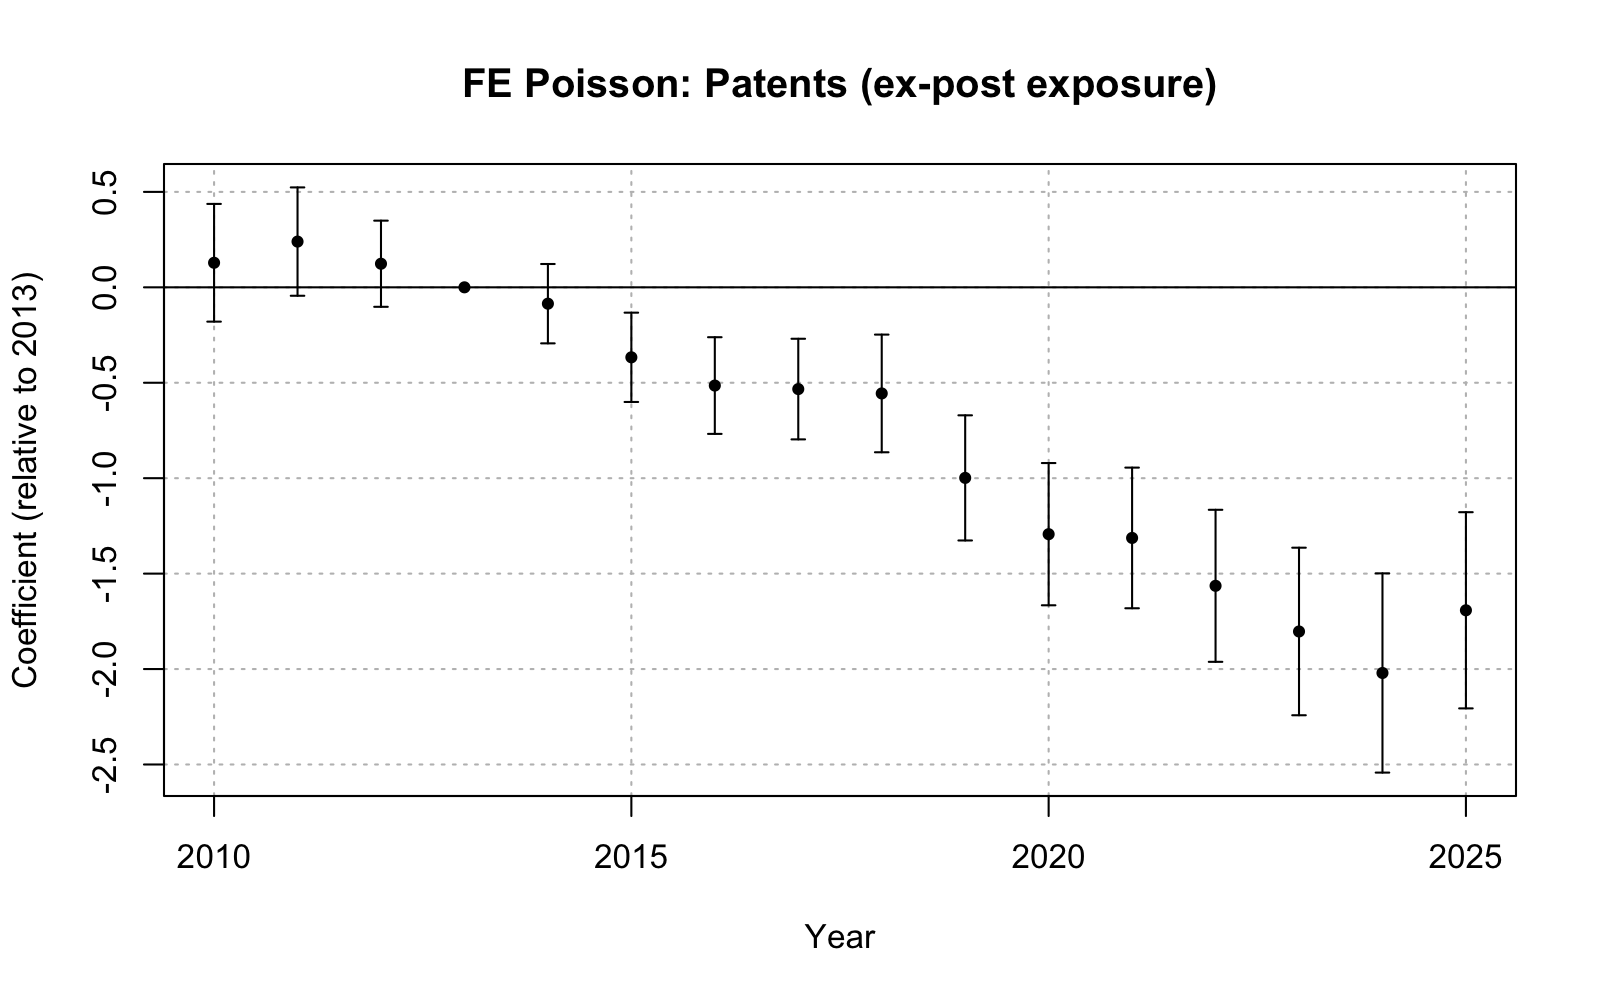
\includegraphics[width=\linewidth]{../output/RQ1/patent_poi_expost.png}
  \caption{FE Poisson event study: patents, ex-post Medicaid exposure}
  \label{fig:rob_rq1_patent_poi_expost}
\end{figure}

\begin{figure}[!h]
  \centering
  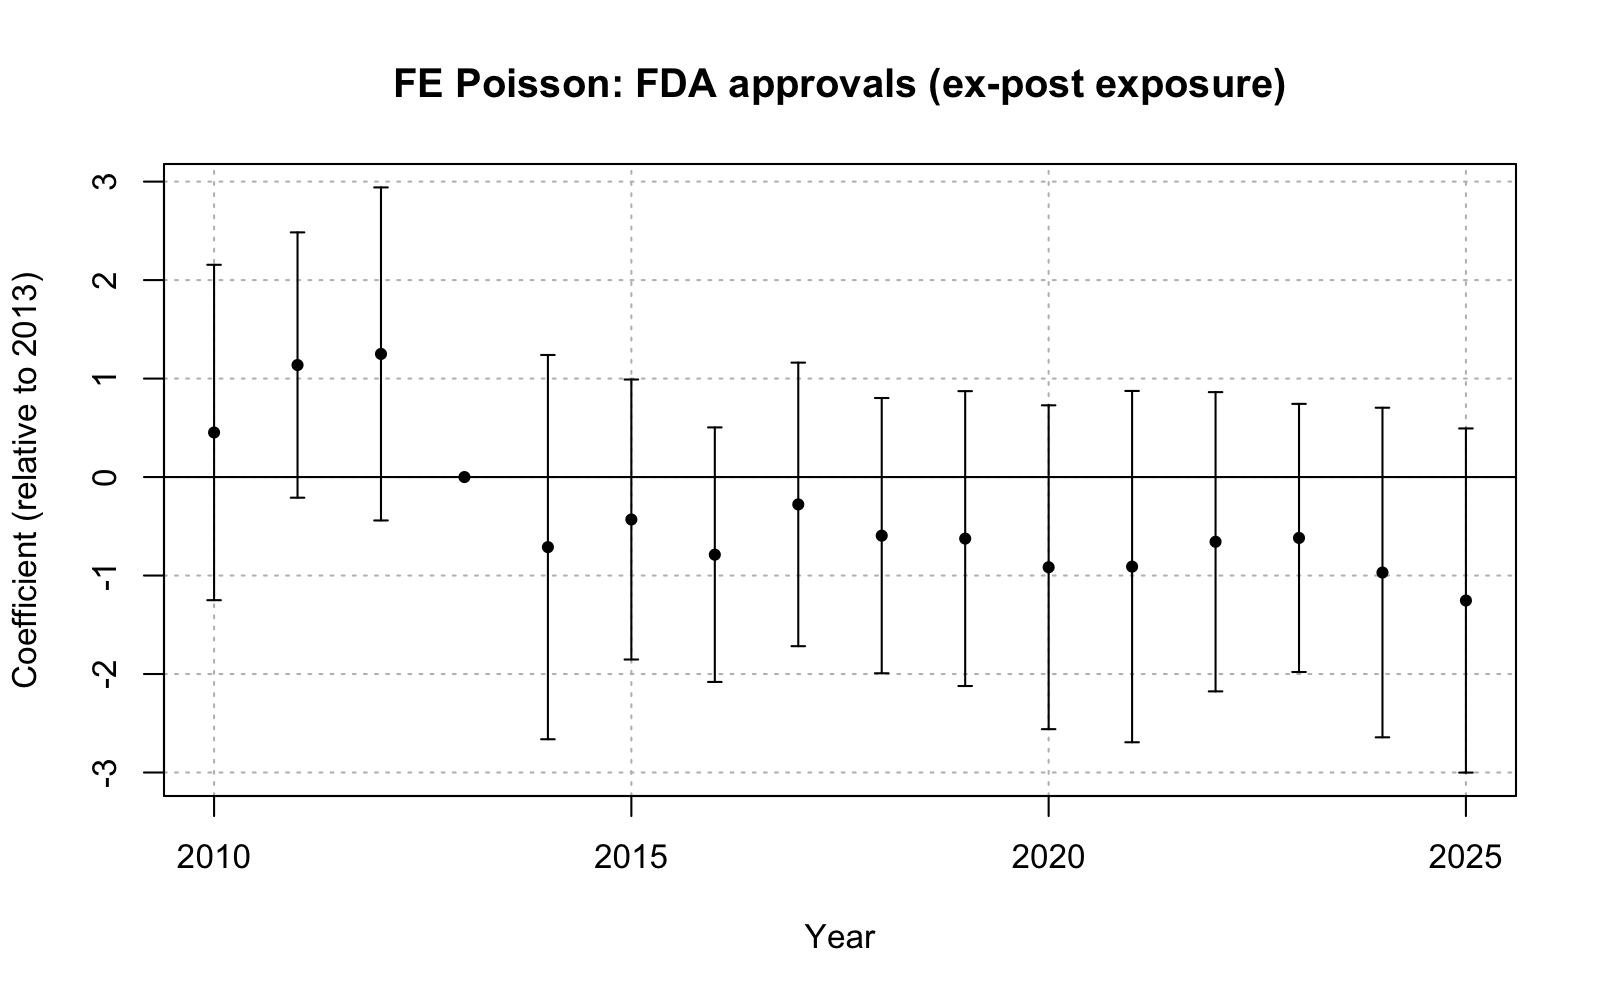
\includegraphics[width=\linewidth]{../output/RQ1/fda_poi_expost.png}
  \caption{FE Poisson event study: FDA approvals, ex-post Medicaid exposure}
  \label{fig:rob_rq1_fda_poi_expost}
\end{figure}

\clearpage

\subsubsection{RQ1: Binned Treatment}

%TC:ignore
\makeatletter
\renewenvironment{table}[1][H]{\@float{table}[H]}{\end@float}
\makeatother
\begin{table}[htbp]
\centering
\caption{Pre-expansion Medicaid market shares and bin assignments}
\label{tab:atc_bins}
\begin{tabular}{llrl}
\toprule
\multicolumn{1}{c}{ATC} & \multicolumn{1}{c}{Therapeutic Area} & \multicolumn{1}{c}{Medicaid Share} & \multicolumn{1}{c}{Bin} \\
\midrule
N & Nervous system                  & 0.363 & High   \\
C & Cardiovascular system           & 0.215 & High   \\
J & Anti-infectives for systemic use & 0.120 & Medium \\
D & Dermatologicals                 & 0.099 & Medium \\
R & Respiratory system              & 0.085 & Low    \\
A & Alimentary tract and metabolism & 0.068 & Low    \\
M & Musculo-skeletal system         & 0.015 & Low    \\
H & Systemic hormonal preparations  & 0.012 & Low    \\
L & Antineoplastic and immunomodulating agents & 0.006 & Low \\
G & Genito-urinary system and sex hormones     & 0.006 & Low \\
S & Sensory organs                  & 0.005 & Low    \\
B & Blood and blood-forming organs  & 0.005 & Low    \\
V & Various                         & 0.000 & Low    \\
P & Antiparasitic products          & 0.000 & Low    \\
\bottomrule
\end{tabular}
\end{table}

\renewenvironment{table}[1][]{}{}
%TC:endignore

%TC:ignore
\footnotesize
\begin{table}
\centering
\begin{talltblr}[         %% tabularray outer open
entry=none,label=none,
note{}={* p \num{< 0.05}, ** p \num{< 0.01}, *** p \num{< 0.001}},
]                     %% tabularray outer close
{                     %% tabularray inner open
width=\linewidth,
colspec={Q[]X[]X[]X[]X[]},
column{2,3,4,5}={}{halign=c,},
column{1}={}{halign=l,},
hline{33}={1,2,3,4,5}{solid, black, 0.05em},
}                     %% tabularray inner close
\toprule
& \SetCell[c=2]{c} Patents && \SetCell[c=2]{c} FDA Approvals & \\
& Medium Bin & High Bin & Medium Bin & High Bin \\ \midrule
2010 & \num{-0.008}    & \num{-0.029}    & \num{0.042}   & \num{0.085}   \\
     & (\num{0.006})   & (\num{0.017})   & (\num{0.055}) & (\num{0.140}) \\
2011 & \num{-0.005}    & \num{-0.025}    & \num{0.058}   & \num{-0.064}  \\
     & (\num{0.006})   & (\num{0.016})   & (\num{0.065}) & (\num{0.105}) \\
2012 & \num{0.009}     & \num{-0.003}    & \num{0.042}   & \num{0.033}   \\
     & (\num{0.006})   & (\num{0.012})   & (\num{0.077}) & (\num{0.121}) \\
2014 & \num{0.015}**   & \num{-0.002}    & \num{0.047}   & \num{-0.091}  \\
     & (\num{0.005})   & (\num{0.011})   & (\num{0.067}) & (\num{0.130}) \\
2015 & \num{0.002}     & \num{-0.027}*   & \num{0.006}   & \num{-0.005}  \\
     & (\num{0.005})   & (\num{0.013})   & (\num{0.073}) & (\num{0.148}) \\
2016 & \num{0.007}     & \num{-0.058}*** & \num{0.158}   & \num{0.070}   \\
     & (\num{0.006})   & (\num{0.014})   & (\num{0.101}) & (\num{0.130}) \\
2017 & \num{0.005}     & \num{-0.047}**  & \num{0.239}*  & \num{0.326}   \\
     & (\num{0.006})   & (\num{0.015})   & (\num{0.114}) & (\num{0.181}) \\
2018 & \num{-0.009}    & \num{-0.075}*** & \num{0.185}*  & \num{0.213}   \\
     & (\num{0.006})   & (\num{0.017})   & (\num{0.093}) & (\num{0.155}) \\
2019 & \num{-0.004}    & \num{-0.092}*** & \num{0.071}   & \num{0.206}   \\
     & (\num{0.007})   & (\num{0.017})   & (\num{0.077}) & (\num{0.162}) \\
2020 & \num{-0.003}    & \num{-0.108}*** & \num{0.012}   & \num{0.141}   \\
     & (\num{0.006})   & (\num{0.018})   & (\num{0.092}) & (\num{0.142}) \\
2021 & \num{-0.005}    & \num{-0.118}*** & \num{0.127}   & \num{-0.048}  \\
     & (\num{0.006})   & (\num{0.018})   & (\num{0.105}) & (\num{0.182}) \\
2022 & \num{-0.010}    & \num{-0.129}*** & \num{0.101}   & \num{0.040}   \\
     & (\num{0.006})   & (\num{0.018})   & (\num{0.075}) & (\num{0.184}) \\
2023 & \num{-0.011}    & \num{-0.141}*** & \num{0.152}   & \num{0.154}   \\
     & (\num{0.006})   & (\num{0.019})   & (\num{0.087}) & (\num{0.182}) \\
2024 & \num{-0.005}    & \num{-0.142}*** & \num{0.037}   & \num{0.070}   \\
     & (\num{0.010})   & (\num{0.019})   & (\num{0.066}) & (\num{0.146}) \\
2025 & \num{-0.020}**  & \num{-0.155}*** & \num{0.010}   & \num{0.032}   \\
     & (\num{0.006})   & (\num{0.019})   & (\num{0.067}) & (\num{0.153}) \\
Num. obs. & \SetCell[c=2]{c} \num{5281696} && \SetCell[c=2]{c} \num{151200} & \\
R2        & \SetCell[c=2]{c} \num{0.534}   && \SetCell[c=2]{c} \num{0.609}  & \\
\bottomrule
\end{talltblr}
\end{table}

\captionof{table}{Binned treatment event-study estimates (FEOLS, ex-ante)}
\label{tab:rob_binned}
\normalsize
%TC:endignore

\begin{figure}[!h]
  \centering
  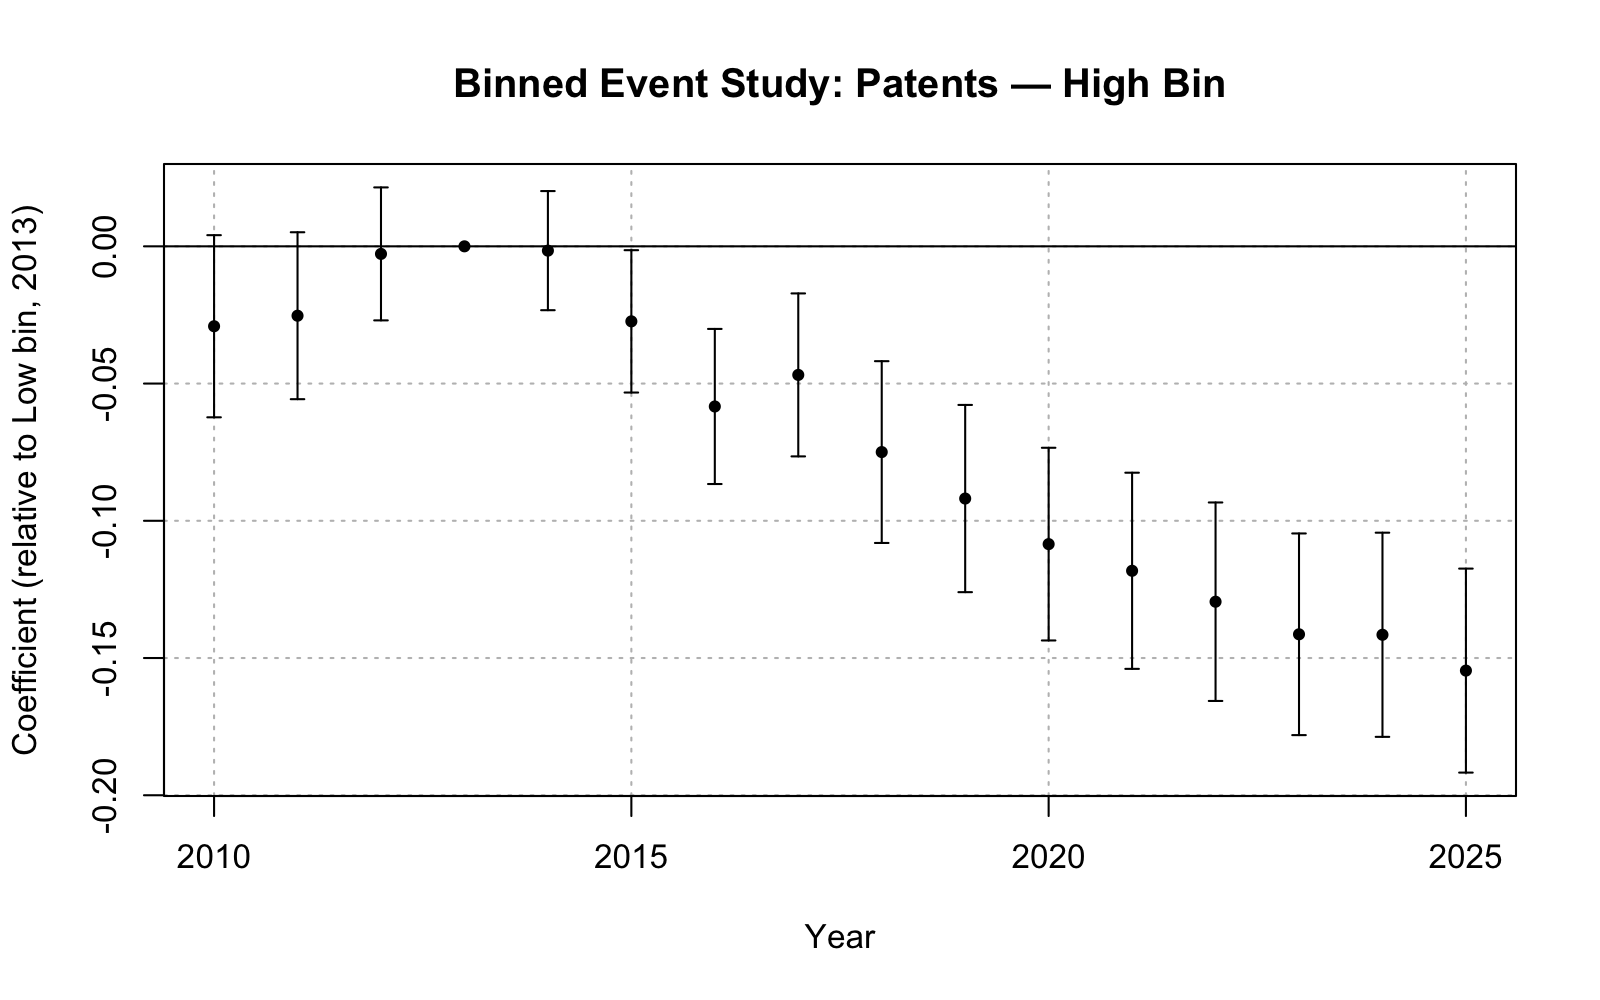
\includegraphics[width=\linewidth]{../output/robustness/binned_treatment/binned_patent_high_es.png}
  \caption{Binned event study: patents, high-exposure bin (N, C)}
  \label{fig:rob_binned_patent_high}
\end{figure}

\begin{figure}[!h]
  \centering
  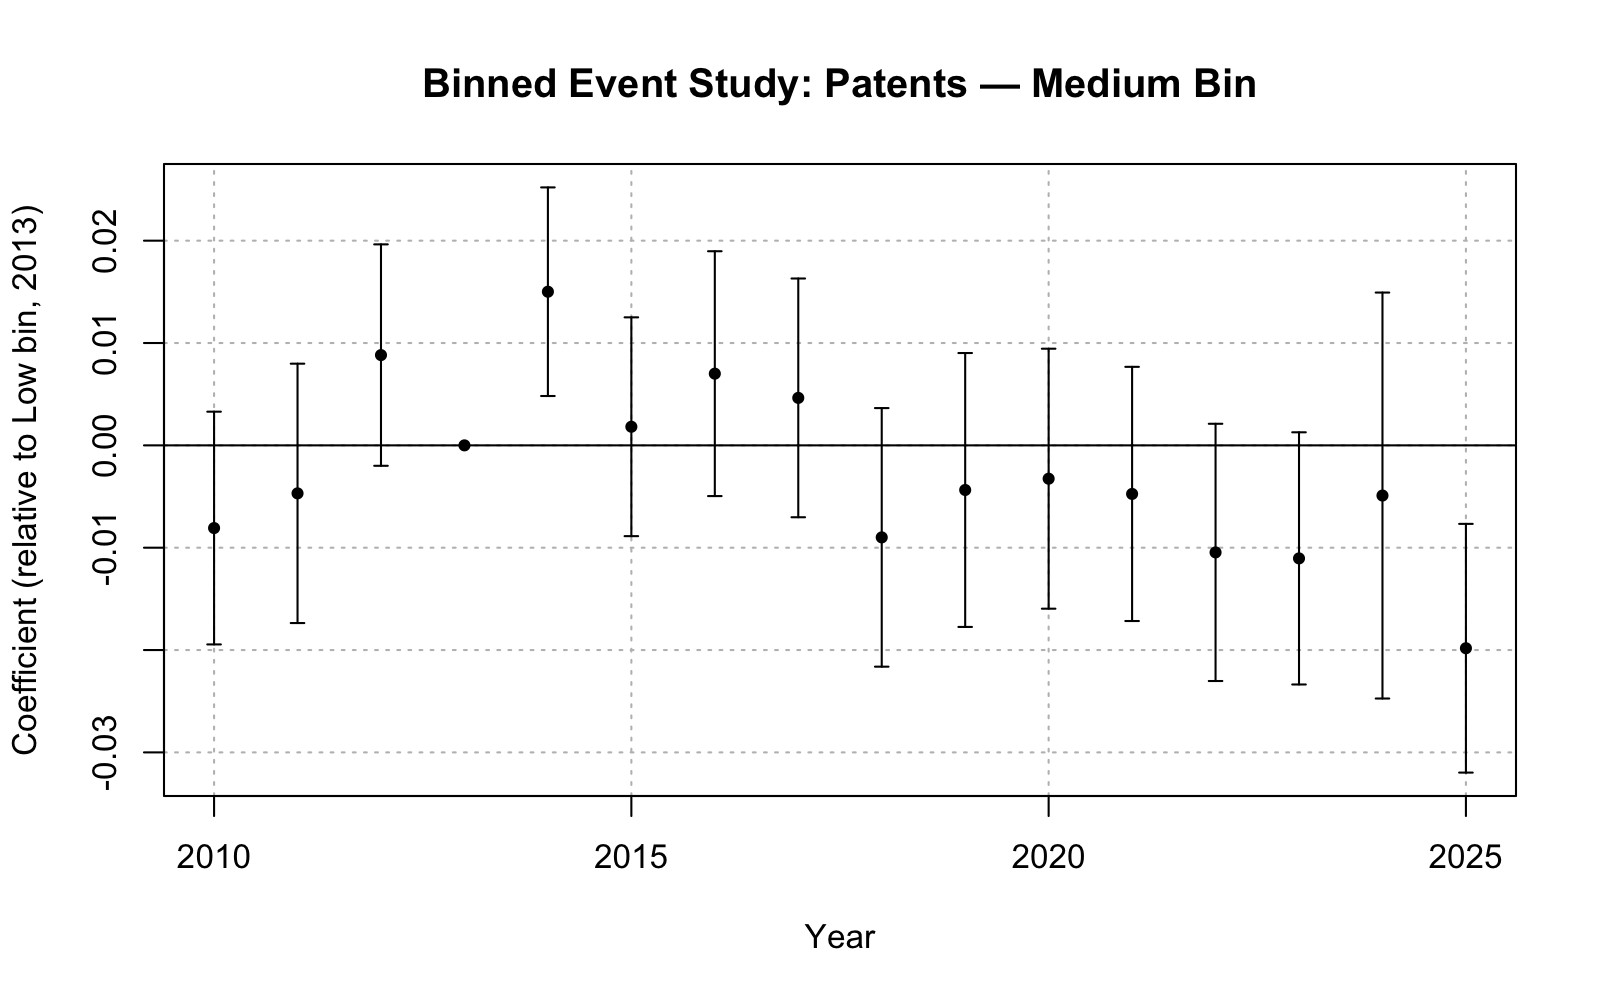
\includegraphics[width=\linewidth]{../output/robustness/binned_treatment/binned_patent_medium_es.png}
  \caption{Binned event study: patents, medium-exposure bin (J, D)}
  \label{fig:rob_binned_patent_medium}
\end{figure}

\clearpage

\begin{figure}[!h]
  \centering
  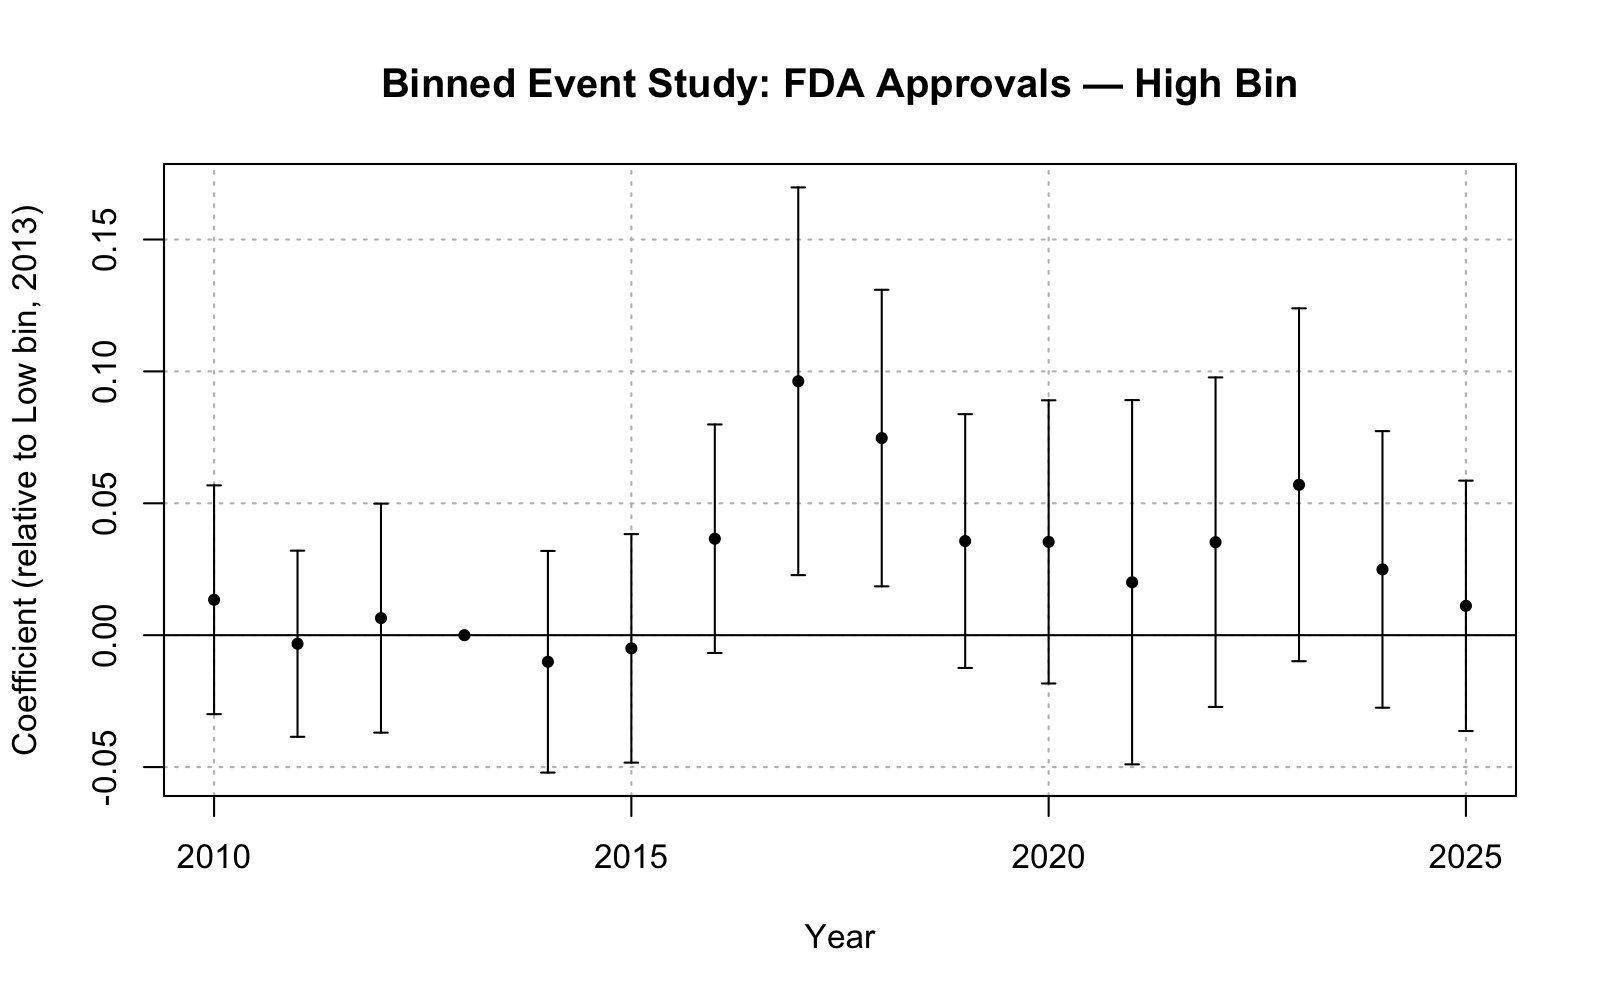
\includegraphics[width=\linewidth]{../output/robustness/binned_treatment/binned_fda_high_es.png}
  \caption{Binned event study: FDA approvals, high-exposure bin (N, C)}
  \label{fig:rob_binned_fda_high}
\end{figure}

\begin{figure}[!h]
  \centering
  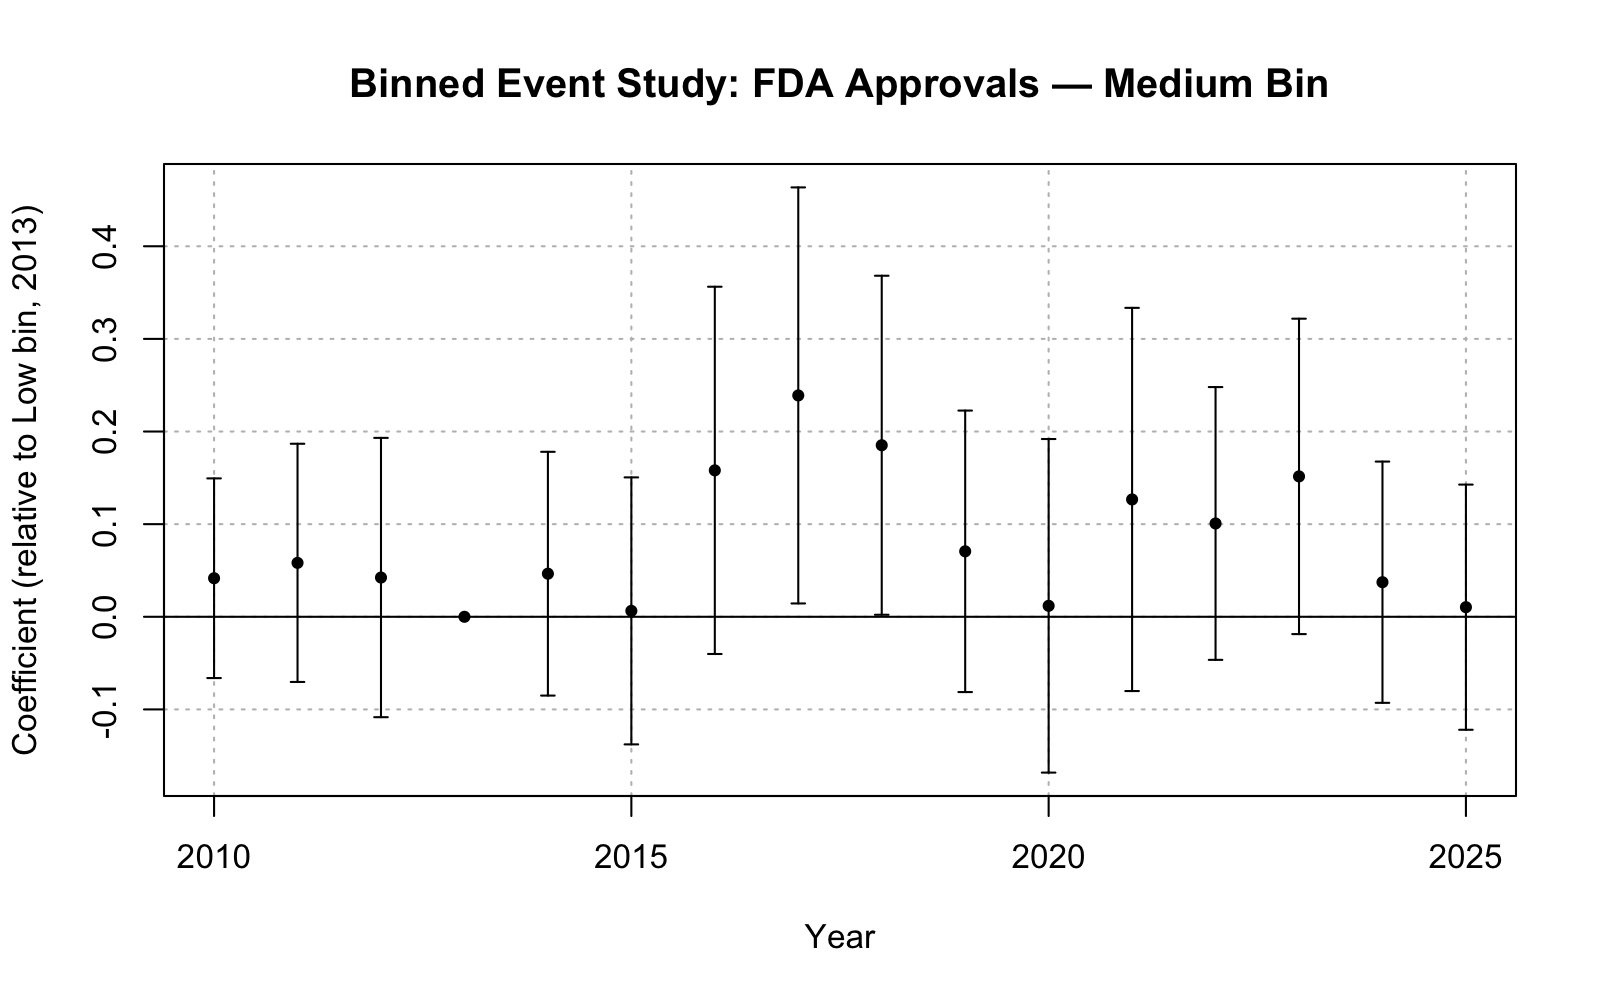
\includegraphics[width=\linewidth]{../output/robustness/binned_treatment/binned_fda_medium_es.png}
  \caption{Binned event study: FDA approvals, medium-exposure bin (J, D)}
  \label{fig:rob_binned_fda_medium}
\end{figure}

\clearpage

\subsubsection{RQ1: Continuous Difference-in-Differences}

%TC:ignore
\makeatletter
\renewenvironment{table}[1][H]{\@float{table}[H]}{\end@float}
\makeatother
\footnotesize
\begin{table}
\centering
\begin{talltblr}[         %% tabularray outer open
entry=none,label=none,
note{}={* 95\% uniform confidence band does not cover 0},
]                     %% tabularray outer close
{                     %% tabularray inner open
colspec={Q[]Q[]Q[]},
column{2,3}={}{halign=c,},
column{1}={}{halign=l,},
hline{8}={1,2,3}{solid, black, 0.05em},
}                     %% tabularray inner close
\toprule
Event Time & Patents & FDA Approvals \\ \midrule %% TinyTableHeader
-3 & \num{0.0038} & \num{-0.0368} \\
   & (\num{0.0034}) & (\num{0.0602}) \\
-2 & \num{0.0023} & \num{0.0361} \\
   & (\num{0.0037}) & (\num{0.0576}) \\
-1 & \num{0.0002} & \num{-0.0326} \\
   & (\num{0.0050}) & (\num{0.0632}) \\
0 & \num{-0.0025} & \num{-0.0506} \\
   & (\num{0.0044}) & (\num{0.0731}) \\
1 & \num{-0.0126} & \num{-0.0092} \\
   & (\num{0.0055}) & (\num{0.0706}) \\
2 & \num{-0.0181}* & \num{0.0646} \\
   & (\num{0.0062}) & (\num{0.0721}) \\
3 & \num{-0.0165} & \num{0.2233} \\
   & (\num{0.0069}) & (\num{0.1018}) \\
4 & \num{-0.0189} & \num{0.1568} \\
   & (\num{0.0073}) & (\num{0.0930}) \\
5 & \num{-0.0271}* & \num{0.0861} \\
   & (\num{0.0080}) & (\num{0.0866}) \\
6 & \num{-0.0313}* & \num{0.1151} \\
   & (\num{0.0082}) & (\num{0.0846}) \\
7 & \num{-0.0315}* & \num{0.0223} \\
   & (\num{0.0084}) & (\num{0.1022}) \\
8 & \num{-0.0333}* & \num{0.0579} \\
   & (\num{0.0083}) & (\num{0.1086}) \\
9 & \num{-0.0348}* & \num{0.1329} \\
   & (\num{0.0084}) & (\num{0.1056}) \\
10 & \num{-0.0358}* & \num{0.0404} \\
   & (\num{0.0085}) & (\num{0.0921}) \\
11 & \num{-0.0324}* & \num{-0.0213} \\
   & (\num{0.0091}) & (\num{0.0919}) \\
\bottomrule
\end{talltblr}
\end{table}

\normalsize
\renewenvironment{table}[1][]{}{}
%TC:endignore

\begin{figure}[!h]
  \centering
  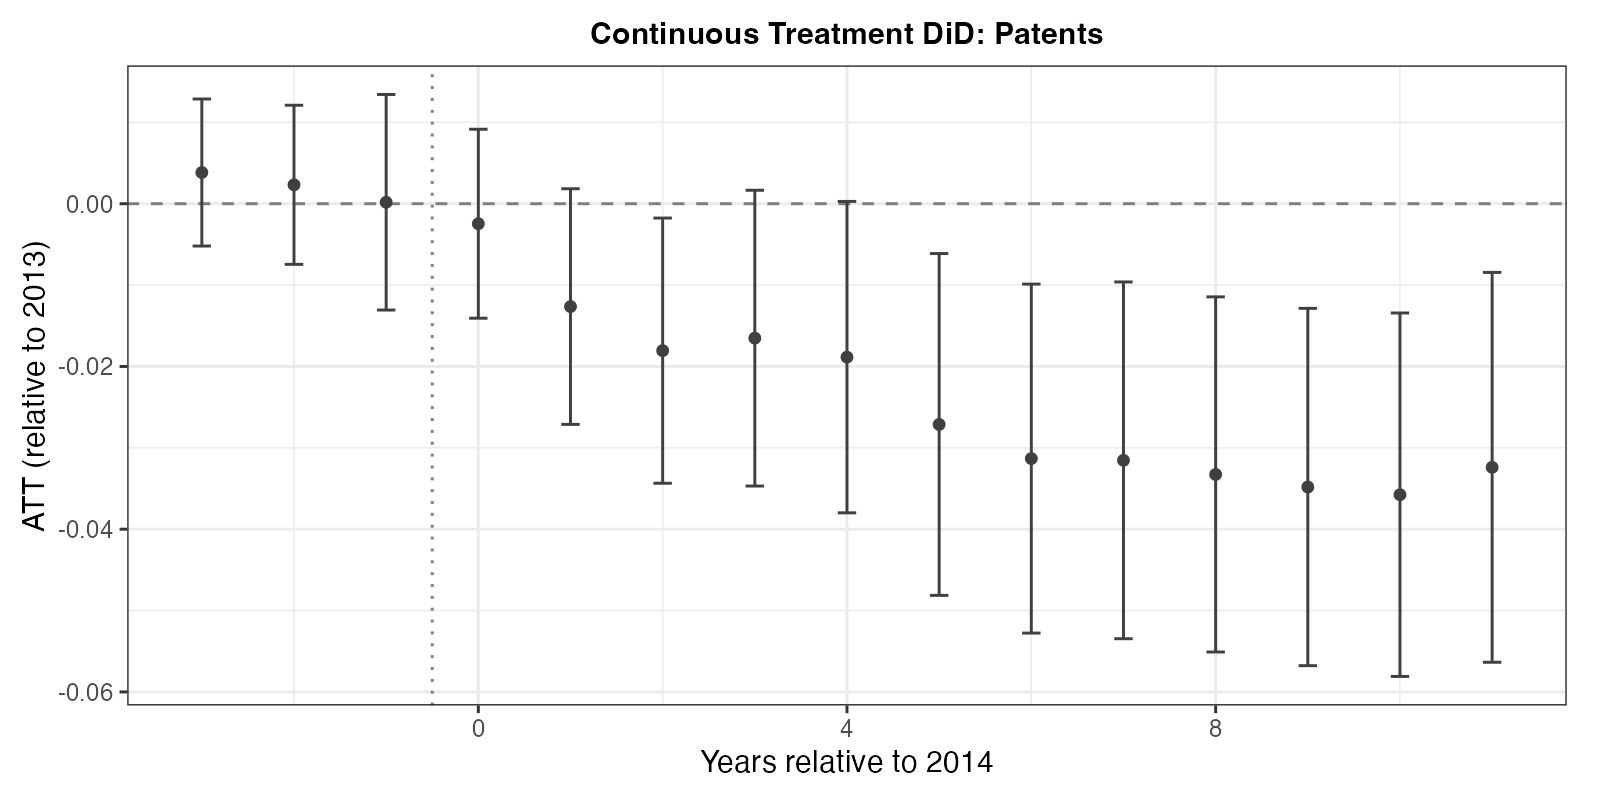
\includegraphics[width=\linewidth]{../output/robustness/contdid/contdid_patent_es.png}
  \caption{Continuous DiD event study: patents}
  \label{fig:rob_contdid_patent}
\end{figure}

\begin{figure}[!h]
  \centering
  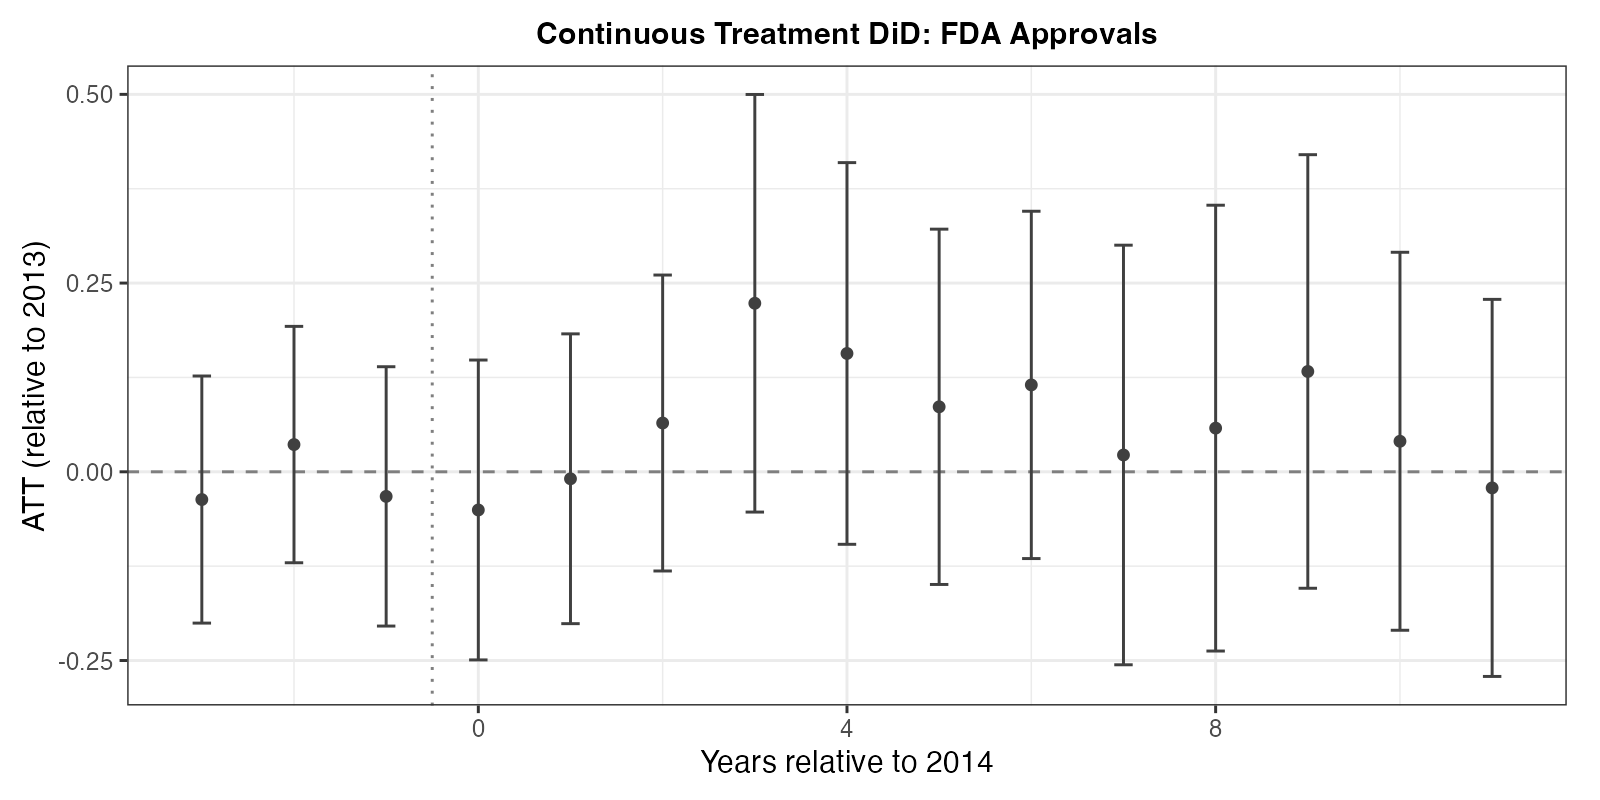
\includegraphics[width=\linewidth]{../output/robustness/contdid/contdid_fda_es.png}
  \caption{Continuous DiD event study: FDA approvals}
  \label{fig:rob_contdid_fda}
\end{figure}

\clearpage

\subsubsection{RQ2: Ex-Post FEOLS}

%TC:ignore
\footnotesize
\begin{table}
\centering
\begin{talltblr}[         %% tabularray outer open
entry=none,label=none,
note{}={* p \num{< 0.05}, ** p \num{< 0.01}, *** p \num{< 0.001}},
]                     %% tabularray outer close
{                     %% tabularray inner open
width=\linewidth,
colspec={Q[]X[]X[]X[]X[]},
column{2,3,4,5}={}{halign=c,},
column{1}={}{halign=l,},
hline{33}={1,2,3,4,5}{solid, black, 0.05em},
}                     %% tabularray inner close
\toprule
& \SetCell[c=2]{c} Patents && \SetCell[c=2]{c} FDA Approvals & \\
& Medicaid Market Share & PDL Exposure & Medicaid Market Share & PDL Exposure \\ \midrule
2010 & \num{-0.033}    & \num{1.546}     & \num{0.285}   & \num{0.046}   \\
     & (\num{0.035})   & (\num{2.018})   & (\num{0.448}) & (\num{0.807}) \\
2011 & \num{-0.010}    & \num{0.734}     & \num{0.344}   & \num{-0.257}  \\
     & (\num{0.033})   & (\num{1.642})   & (\num{0.412}) & (\num{0.711}) \\
2012 & \num{0.005}     & \num{1.079}     & \num{0.371}   & \num{1.395}   \\
     & (\num{0.027})   & (\num{1.289})   & (\num{0.447}) & (\num{0.912}) \\
2014 & \num{-0.017}    & \num{4.161}*    & \num{-0.338}  & \num{0.398}   \\
     & (\num{0.024})   & (\num{1.890})   & (\num{0.536}) & (\num{0.647}) \\
2015 & \num{-0.088}**  & \num{0.836}     & \num{-0.037}  & \num{1.158}   \\
     & (\num{0.027})   & (\num{1.480})   & (\num{0.422}) & (\num{0.881}) \\
2016 & \num{-0.123}*** & \num{-1.554}    & \num{0.456}   & \num{2.642}   \\
     & (\num{0.032})   & (\num{1.620})   & (\num{0.418}) & (\num{1.682}) \\
2017 & \num{-0.123}*** & \num{-1.342}    & \num{1.566}*  & \num{1.924}   \\
     & (\num{0.034})   & (\num{1.890})   & (\num{0.690}) & (\num{0.992}) \\
2018 & \num{-0.136}*** & \num{-2.787}    & \num{1.181}*  & \num{1.683}   \\
     & (\num{0.037})   & (\num{1.644})   & (\num{0.563}) & (\num{1.021}) \\
2019 & \num{-0.195}*** & \num{-3.807}*   & \num{0.359}   & \num{1.171}*  \\
     & (\num{0.039})   & (\num{1.912})   & (\num{0.498}) & (\num{0.591}) \\
2020 & \num{-0.227}*** & \num{-4.650}*   & \num{0.598}   & \num{1.585}   \\
     & (\num{0.041})   & (\num{1.894})   & (\num{0.537}) & (\num{0.942}) \\
2021 & \num{-0.224}*** & \num{-5.267}**  & \num{0.103}   & \num{3.110}*  \\
     & (\num{0.040})   & (\num{1.687})   & (\num{0.583}) & (\num{1.393}) \\
2022 & \num{-0.235}*** & \num{-6.029}**  & \num{0.381}   & \num{0.994}   \\
     & (\num{0.041})   & (\num{1.941})   & (\num{0.593}) & (\num{0.653}) \\
2023 & \num{-0.240}*** & \num{-6.926}*** & \num{0.798}   & \num{1.191}   \\
     & (\num{0.041})   & (\num{1.851})   & (\num{0.583}) & (\num{1.737}) \\
2024 & \num{-0.252}*** & \num{-6.485}*** & \num{0.154}   & \num{-0.447}  \\
     & (\num{0.042})   & (\num{1.788})   & (\num{0.501}) & (\num{0.589}) \\
2025 & \num{-0.212}*** & \num{-4.589}**  & \num{-0.347}  & \num{-1.113}  \\
     & (\num{0.041})   & (\num{1.549})   & (\num{0.525}) & (\num{0.908}) \\
Num. obs. & \SetCell[c=2]{c} \num{5281696} && \SetCell[c=2]{c} \num{151200} & \\
R2        & \SetCell[c=2]{c} \num{0.535}   && \SetCell[c=2]{c} \num{0.609}  & \\
\bottomrule
\end{talltblr}
\end{table}

\captionof{table}{FEOLS event-study estimates: Medicaid demand and PDL exposure (ex-post)}
\label{tab:rob_rq2_feols_expost}
\normalsize
%TC:endignore

\begin{figure}[!h]
  \centering
  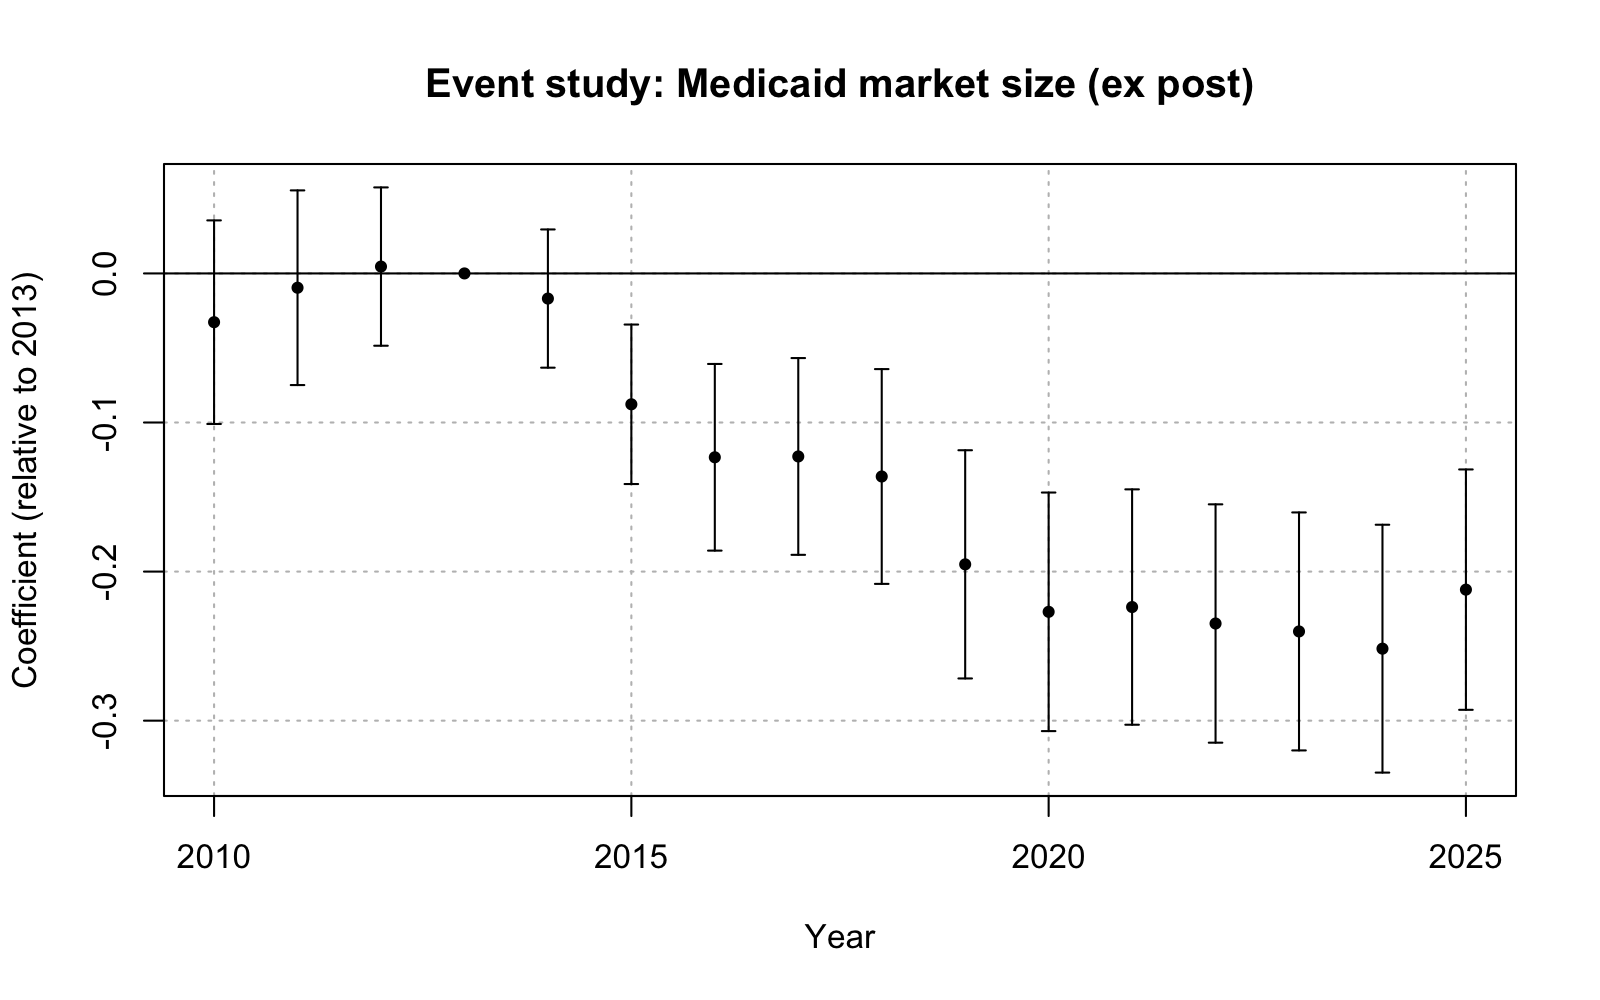
\includegraphics[width=\linewidth]{../output/RQ2/patent_feols_expost_medicaid.png}
  \caption{FEOLS event study: patents, Medicaid exposure (ex-post)}
  \label{fig:rob_rq2_patent_expost_medicaid}
\end{figure}

\begin{figure}[!h]
  \centering
  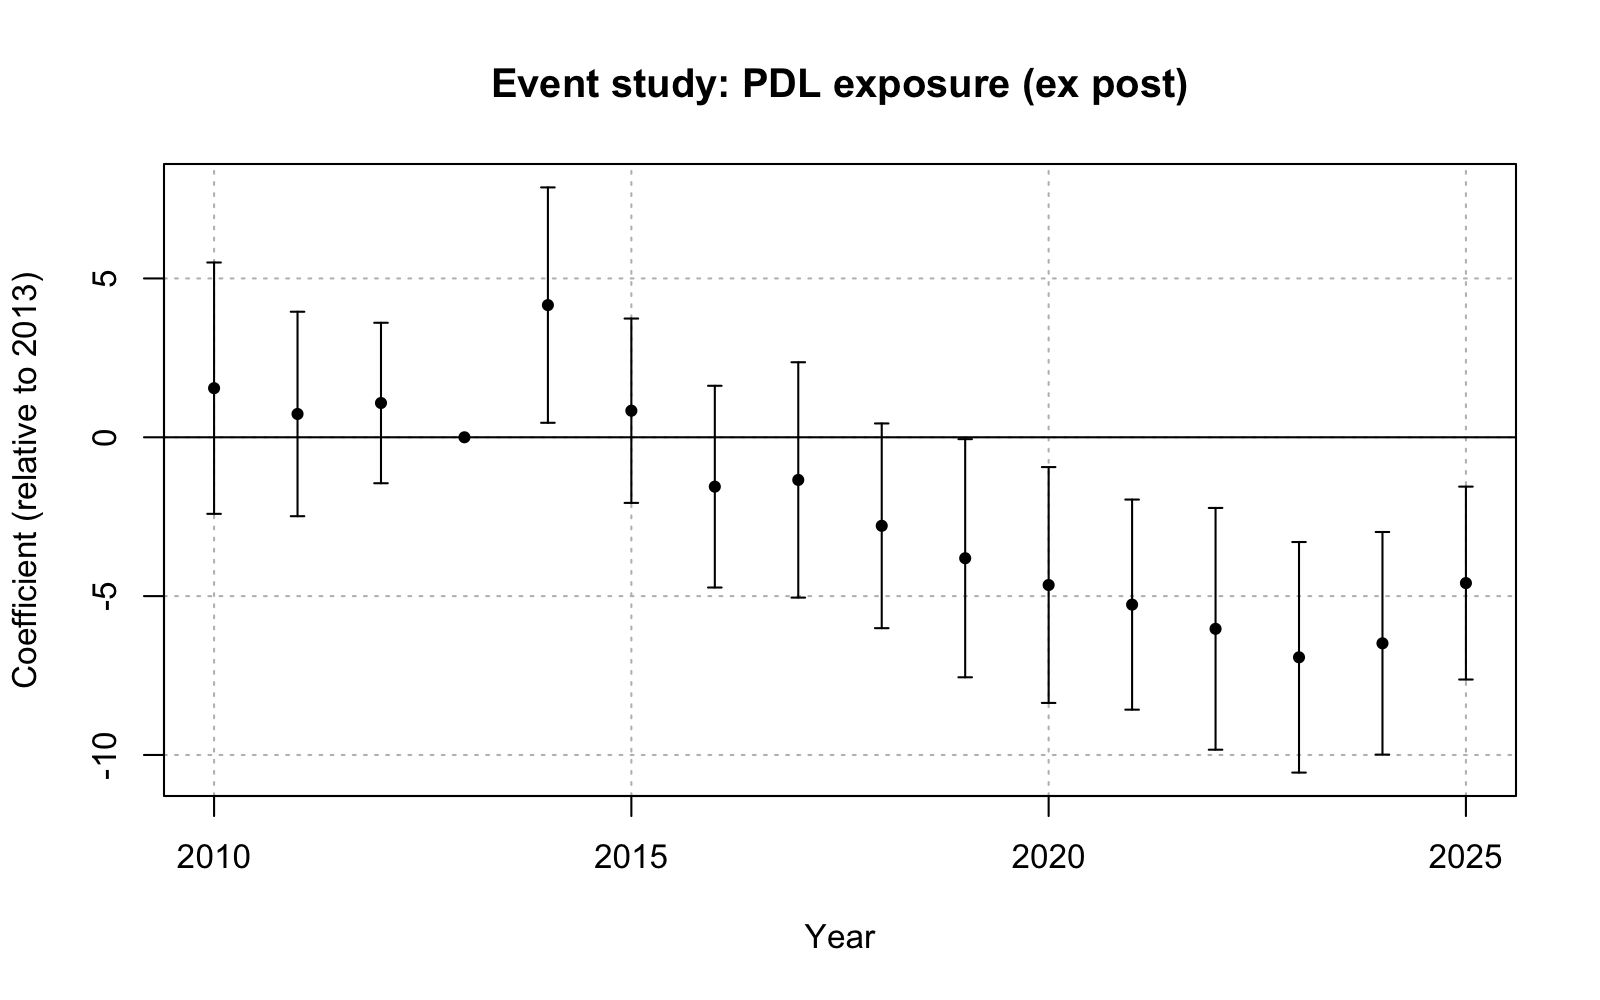
\includegraphics[width=\linewidth]{../output/RQ2/patent_feols_expost_pdl.png}
  \caption{FEOLS event study: patents, PDL exposure (ex-post)}
  \label{fig:rob_rq2_patent_expost_pdl}
\end{figure}

\clearpage

\begin{figure}[!h]
  \centering
  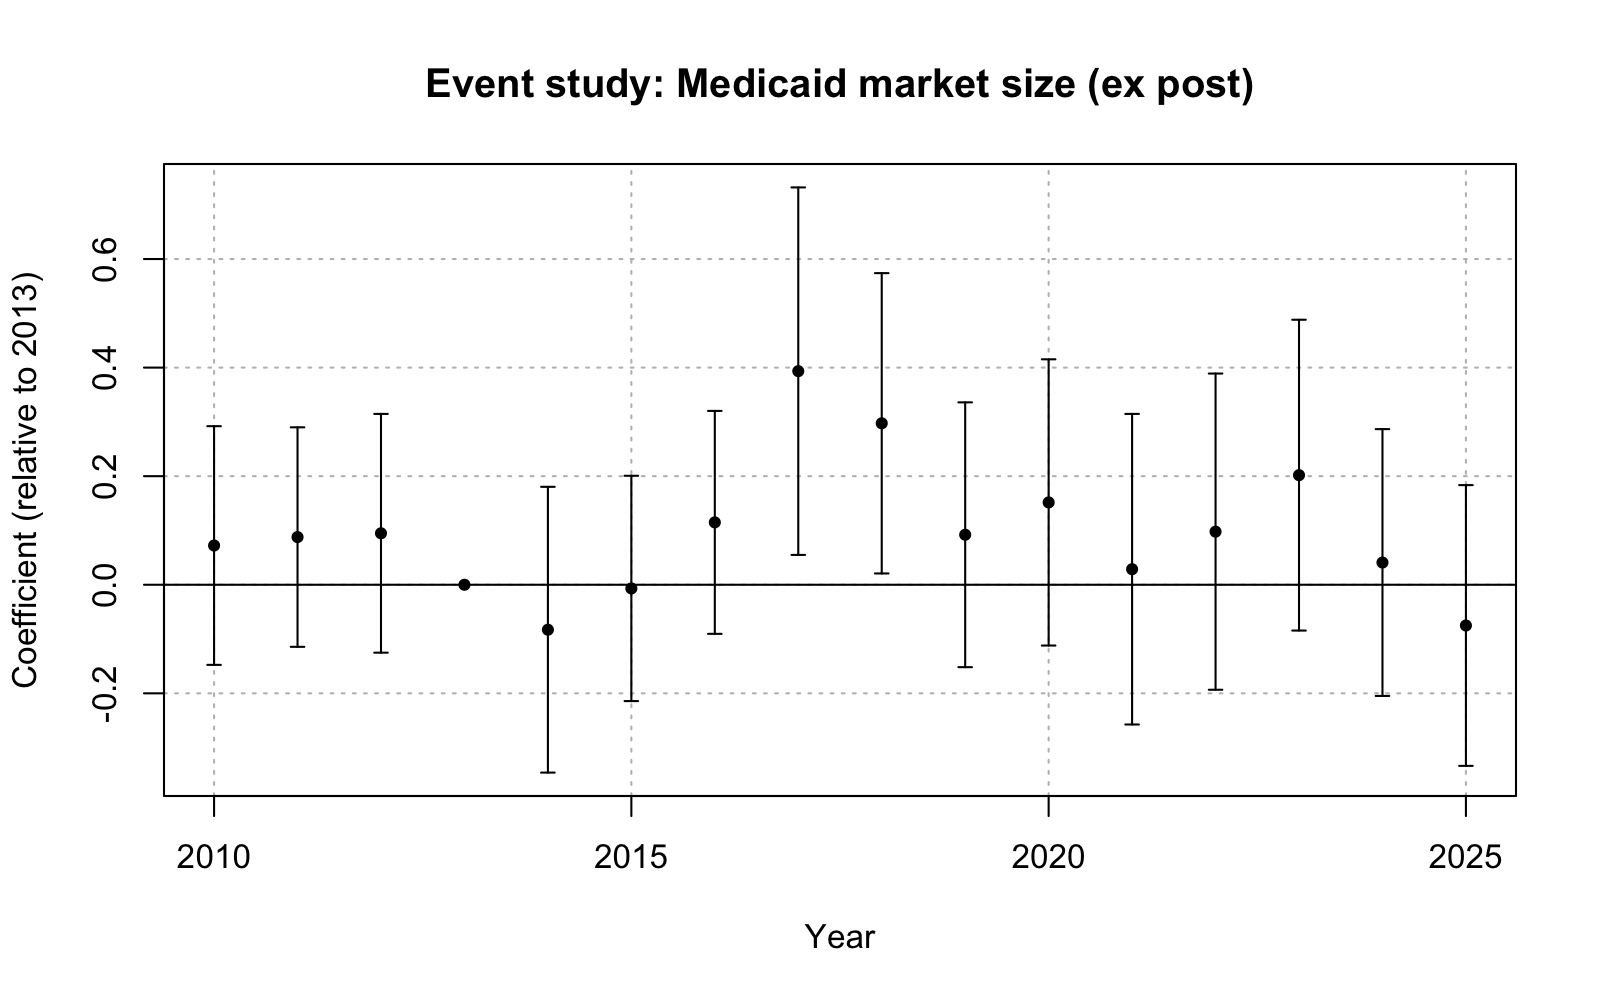
\includegraphics[width=\linewidth]{../output/RQ2/fda_feols_expost_medicaid.png}
  \caption{FEOLS event study: FDA approvals, Medicaid exposure (ex-post)}
  \label{fig:rob_rq2_fda_expost_medicaid}
\end{figure}

\begin{figure}[!h]
  \centering
  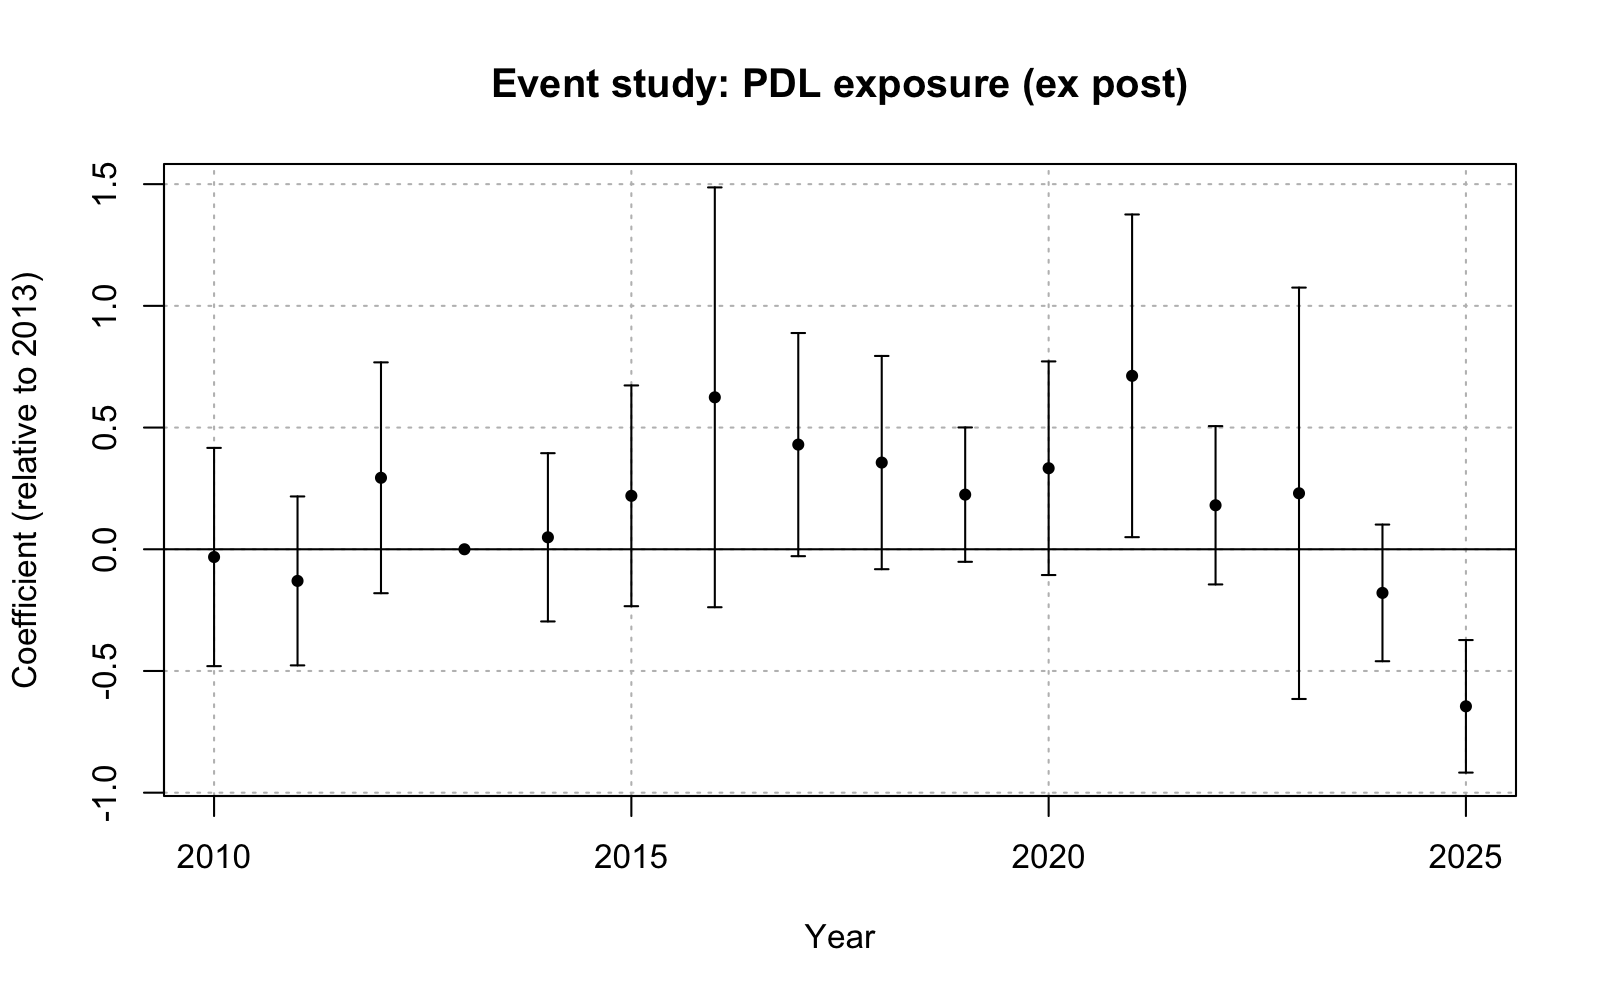
\includegraphics[width=\linewidth]{../output/RQ2/fda_feols_expost_pdl.png}
  \caption{FEOLS event study: FDA approvals, PDL exposure (ex-post)}
  \label{fig:rob_rq2_fda_expost_pdl}
\end{figure}

\clearpage

\subsubsection{RQ3: Ex-Post FEOLS}

%TC:ignore
\footnotesize
\begin{table}
\centering
\begin{talltblr}[         %% tabularray outer open
entry=none,label=none,
note{}={* p \num{< 0.05}, ** p \num{< 0.01}, *** p \num{< 0.001}},
]                     %% tabularray outer close
{                     %% tabularray inner open
colspec={Q[]Q[]Q[]},
column{2,3}={}{halign=c,},
column{1}={}{halign=l,},
hline{26}={1,2,3}{solid, black, 0.05em},
}                     %% tabularray inner close
\toprule
& Patents & FDA Approvals \\ \midrule
Medicaid Share × ATC = A & \num{-0.157}*** & \num{1.301}**  \\
& (\num{0.031})   & (\num{0.420})  \\
Medicaid Share × ATC = B & \num{0.151}***  & \num{-0.121}   \\
& (\num{0.027})   & (\num{0.784})  \\
Medicaid Share × ATC = C & \num{-0.094}*** & \num{0.373}    \\
& (\num{0.015})   & (\num{0.278})  \\
Medicaid Share × ATC = D & \num{-0.017}    & \num{0.881}**  \\
& (\num{0.062})   & (\num{0.337})  \\
Medicaid Share × ATC = G & \num{0.032}     & \num{-1.058}   \\
& (\num{0.049})   & (\num{1.121})  \\
Medicaid Share × ATC = H & \num{0.619}***  & \num{0.446}    \\
& (\num{0.096})   & (\num{0.530})  \\
Medicaid Share × ATC = J & \num{0.035}     & \num{-0.078}   \\
& (\num{0.034})   & (\num{0.089})  \\
Medicaid Share × ATC = L & \num{0.443}     & \num{-0.244}   \\
& (\num{0.578})   & (\num{2.115})  \\
Medicaid Share × ATC = M & \num{-0.212}*** & \num{0.017}    \\
& (\num{0.048})   & (\num{0.858})  \\
Medicaid Share × ATC = N & \num{-0.174}*** & \num{0.047}    \\
& (\num{0.039})   & (\num{0.101})  \\
Medicaid Share × ATC = R & \num{0.005}     & \num{0.178}    \\
& (\num{0.003})   & (\num{0.130})  \\
Medicaid Share × ATC = S & \num{0.105}***  & \num{6.473}*   \\
& (\num{0.020})   & (\num{3.004})  \\
Num. obs.                & \num{19617728}  & \num{561600}   \\
R2                       & \num{0.247}     & \num{0.235}    \\
\bottomrule
\end{talltblr}
\end{table}

\captionof{table}{Triple-difference estimates: therapeutic-class heterogeneity (FEOLS, ex-post)}
\label{tab:rob_rq3_feols_expost}
\normalsize
%TC:endignore

\clearpage

% --- From theoretical_model.tex ---

\subsection{Baseline Model Parameters} \label{app:parameters}

Table~\ref{tab:parameters} reports the baseline parameter values used to generate Figure~\ref{fig:comp_statics}. Parameters that are not varied are held at these baseline values.

%TC:ignore
\makeatletter
\renewenvironment{table}[1][H]{\@float{table}[H]}{\end@float}
\makeatother
\begin{table}[H]
\centering
\caption{Baseline parameter values used for comparative statics simulations}
\label{tab:parameters}
\begin{tblr}{
    width = \textwidth,
    colspec = {X[c,0.8] X[l,3.4] X[c,1.2]},
    row{1} = {halign=c}
}
\toprule
Parameter & Description & Baseline Value \\
\midrule
$\sigma$      & Std.\ dev.\ of the innovation shock $\varepsilon_i$                   & $1.0$           \\
$\bar{a}$     & Clinical quality threshold (P\&T approval bar)                        & $0.5$           \\
$\bar{p}$     & Regulatory price cap                                                  & $10.0$          \\
$\bar{c}$     & Expected marginal cost                                                & $2.0$           \\
$k$           & Effort cost scaling parameter                                         & $1.0$           \\
$\alpha_c$    & Rebate scale parameter                                                & $0.02$          \\
$\beta_c$     & Rebate elasticity under power form $\tau_c = \alpha_c M_c^{\beta_c}$ & $0.75$          \\
$c$           & Marginal cost distribution in the duopoly auction                     & $U[0.5,\, 3.5]$ \\
$M_0$         & Reference market size                                                 & $100$           \\
$\delta$      & Period 2 cost reduction factor                                        & $0.7$           \\
\bottomrule
\end{tblr}
\end{table}
\renewenvironment{table}[1][]{}{}
%TC:endignore

\end{document}
%
}

\begin{document}

% ===== Title Page =====
\begin{titlepage}
  \centering
  \vspace*{3cm}
  {\LARGE\bfseries MPhil Thesis\par}
  \vspace{1.5cm}
  {\Large Mohammad-Shah Karim\par}
  \vspace{1cm}
  {\large May 2026\par}
  \vspace{2cm}
  {\large Word count: \totalwordcount\par}
  \vfill
\end{titlepage}

% ===== Table of Contents =====
\mastertoc
\newpage

% ===== Main Body =====
\documentclass[12pt]{article}
\usepackage{geometry}
\geometry{a4paper, portrait, margin=1in}

% --- Math Packages ---
\usepackage{amsmath}
\usepackage{amssymb}
\usepackage{amsfonts}
\usepackage{amsthm}

% --- Graphics & Diagrams ---
\usepackage{graphicx}
\usepackage{tikz}
\usetikzlibrary{shapes, arrows, positioning}

% --- Formatting ---
\usepackage{parskip}
\usepackage[hidelinks]{hyperref}
\usepackage{natbib}
\usepackage{enumitem}
\pagestyle{plain}

\title{MPhil Thesis: Introduction}
\author{Mohammad-Shah Karim}
\date{April 2026}

\begin{document}

\maketitle

\section{Introduction}

Pharmaceutical innovation is central towards long-run improvements in health and welfare. New drugs can improve quantity of life while changing the treatment possibilities which are available for physicians to administer on patients. At the same time, pharmaceutical innovation is unusually sensitive to policy. Development of a new drug requires a large upfront investment with a long development horizon including patent applications and clinical trials, with only a high probability of failure. Since the returns to a successful drug accrue over multiple years and depend on both prices and the volumes that prevail within the market, the incentives to undertake the investment to develop a drug are shaped not only by opportunity, but also by the economic and institutional environment present which determine the expected future profits once the drug reaches the market.

This makes the pharmaceutical market within the United States of America an ideal setting for studying how public policy shapes scientific opportunity. Federal and state governments are now responsible for roughly half of all prescription drug spending (INSERT SOURCE HERE), both as direct purchasers through programmes such as Medicaid and Medicare, and also indirectly through the tax preferences and regulatory rules that govern private insurance. Medicaid is especially important in this respect - it is a large public buyer, but it does not operate as a standard private insurer. Manufacturers that wish to have Medicaid coverage must participate in the Medicaid Drug rebate Program, and states can use Preferred Drug Lists (PDLs) in order to negotiate additional rebates in exchange for preferred formulary placement. Given this, Medicaid demand passes through a public procurement system with statutory and supplement rebates in addition to state level formulary bargaining, thus it cannot be treated as additional market demand.

This thesis examines the consequences of one of such reforms for pharmaceutical innovation - the 2014 Medicaid expansion under the the Patient Protection and Affordable Care Act (ACA). The reform produced a well-documented expansion in the size of the Medicaid market, with population coverage increasing by close to twenty million enrollees int he years following the policy change (INSERT SOURCE HERE). Under standard market-sized frameworks in the pharmaceutical sector this should increase innovation incentives for drug-classes more exposed to Medicaid demand \citep{finkelstein2004static, dubois2015market}. If firms expect to sell more units after a successful round of innovation, the expected returns to R\&D rise. However, the expansion of Medicaid took place inside a procurement framework that combined two features of that are unusual under the standards of a private insurer. A statutory rebate schedule that mechanically transfers a share of any list-price revenue back to the state, and a state-administered formulary system in which Preferred Drug Lists (PDLs) determine which products are reimbursed without prior authorisation. Thus the institutional features meant that an expansion of Medicaid was not simply a positive demand shock for pharmaceutical firm.

The Medicaid setting therefore complicates the prediction under standard pharmaceutical market-sized frameworks. The ACA did not only expand the number of beneficiaries under Medicaid, but it also raised the statutory rebate percentages and extended rebate obligations to Medicaid managed care. Therefore, the reform increased the size of the public market while also increasing the share of revenue back to the state. Additionally, as Medicaid demand grows, preferred placement on a state PDL becomes more valuable. States can use this to negotiate deeper rebates from manufacturers. The same policy may therefore generate two opposing effects. On the one hand, Medicaid expansion raises demand. On the other hand, it may increase pricing pressure and reduce the surplus that firms can capture from that demand.

This thesis therefore raises the question of whether the ACA-induced Medicaid expansion raised pharmaceutical innovation, and whether the response dependent on a firm's exposure to the Medicaid procurement institutions. Put simply, was the expected positive relationship between market size and innovation weakened when the additional demand flows through a state-wide monopsony. Many current drug-pricing reforms, including recent Medicare negotiation policies, rely on the same basic trade-off: lowering public spending and consumer prices may increase static welfare, but it may also affect the expected returns to future innovation, raising the relevance of this question


\newpage
\bibliographystyle{apalike}
\bibliography{references}

\end{document}

\documentclass[12pt]{article}
\usepackage{geometry}
\geometry{a4paper, portrait, margin=1in}

% --- Math Packages ---
\usepackage{amsmath}
\usepackage{amssymb}
\usepackage{amsfonts}
\usepackage{amsthm}

% --- Graphics & Diagrams ---
\usepackage{graphicx}
\usepackage{tikz}
\usetikzlibrary{shapes, arrows, positioning}

% --- Formatting ---
\usepackage{parskip}
\usepackage[hidelinks]{hyperref}
\usepackage{natbib}
\usepackage{enumitem}
\usepackage{booktabs}
\usepackage{caption}
\usepackage{siunitx}
\usepackage{tabularray}
\UseTblrLibrary{booktabs, siunitx}
\pagestyle{plain}

% --- Word count (requires compiling with --shell-escape) ---
\newcommand{\wordcount}{%
  \immediate\write18{texcount -sum -1 \jobname.tex 2>/dev/null | python3 -c "import sys; n=sys.stdin.read().strip(); print(f'{int(n):,}') if n.isdigit() else print('?')" > \jobname.wc}%
  \input{\jobname.wc}%
}

\title{MPhil Thesis: Literature Review}
\author{Mohammad-Shah Karim}
\date{May 2026}

\begin{document}

\maketitle

\begin{center}
  \small Word count: \wordcount
\end{center}

\tableofcontents

\newpage

\section{Literature Review}

This thesis sits at the intersection of the literature on pharmaceutical innovation and how the institutional settings behind public reimbursement shape firm incentives. It also draws on work examining the timing of innovation measures across the drug-development pipeline

Before turning to these areas, it is beneficial to understand the current studies on the ACA Medicaid expansion. The reform yielded large gains in concentrated in states that chose to expand access to Medicaid, with the gaps in racial and ethnic coverage narrowing as a result \citep{courtemanche2020impact, frean2017premium, miller2019four}. These states saw increased affordability indicating reductions in the cost barriers for accessing healthcare \citep{miller2017health}, alongside declines in medical debt and bankruptcy from healthcare \citep{brevoort2017medicaid, HU201899}. These increases in access and financial welfare were accompanies with improvements in self-reported health and reductions in adult mortality \citep{miller2021medicaid, miller2017health}. However, evidence on labour market effects has been more limited, where no no significant changes were recorded in employment outcomes or physician hours \citep{duggan2019effects, dague2017effect, neprash2021effect}. This thesis studies a less explored dimension of the Medicaid expansion - its effects on pharmaceutical innovation.

\subsection{Market Size and Pharmaceutical Innovation}



\subsection{Medicaid Expansion and Pharmaceutical Innovation}

The most closely related study to this thesis is \cite{NBERw28755}, which examines the impact of the ACA Medicaid expansion on clinical trial activity. With the use of disease condition Medicaid market shares as a proxy for Medicaid exposure, they find no evidence of a significant innovation response through to 2016. They propose that this null result may reflect the lower expected returns associated with Medicaid relative to reforms such as Medicare Part D, due to manufacturer revenue being constrained by the rebates and price controls embedded within the programme.

While this finding is an important starting point to address the question, their analysis leaves several gaps which this thesis addresses. First, the post-expansion window is constrained by both the innovation outcome studied and the length of the post-expansion window. \citeauthor{NBERw28755} investigated clinical trial activity through to 2016, so their estimates only capture the first two years of the Medicaid demand shock. This is short relative to the development horizon for pharmaceutical drug development, which can span between five to twenty years \citep{brown2022clinical}. As a result, the absence of a response in clinical trials cannot distinguish between an innovation effect that is genuinely absent, or one that has affected early stage R\&D decisions but has not reached the clinical trials stage.

Second, the absence of an aggregate clinical-trial response does not confirm whether the innovation effect differs across therapeutic classes. \citet{sutton1998technology} argues that pharmaceutical R\&D is organised around narrow chemically related drug groups rather than broad therapeutic categories, and finds limited persistence in firms' major follow-on successes within these groups. This suggests that therapeutic-class-level aggregates may conceal meaningful heterogeneity in how firms adjust innovation activity. Instead, an insignificant aggregate relationship may be driven by heterogeneous responses across drug classes. Positive R\&D responses may have occurred in classes where the market-size channel dominated, but the aggregate effect may have been offset by negative clinical-trial responses in areas where the expansion weakened innovation incentives.

Third, while \citeauthor{NBERw28755} propose that the lower returns to the Medicaid market may explain the contrast with earlier market-size studies that find positive innovation responses, this explanation lies outside of their empirical design. Specifically, their analysis does not control for the procurement institutions that may affect manufacturer profits, including rebate pressures and formulary placement on Medicaid's PDL.

This thesis addresses these gaps by extending the analysis across the innovation pipeline, across time, and across therapeutic markets. First, this thesis constructs novel panels linking firms to their drugs in Medicaid's State Drug Utilisation Data, and then to their patenting and FDA approval activity. These innovation outcomes bracket the clinical-trial stage examined by \citeauthor{NBERw28755}, allowing earlier and later innovation responses to be considered separately. Second, the impact of the reform is investigated over a substantially longer post-expansion period, with outcome data extending to 2025, whereas \citeauthor{NBERw28755} used data ending in 2016. This extension allows delayed innovation responses to be captured more clearly, which is particularly important given the long development horizon in pharmaceutical R\&D. Third, class-level heterogeneous responses are examined to determine whether the expansion generated different innovation incentives across the therapeutic markets in which firms operated in, rather than restricting the analysis to an average therapeutic-area effect.

\citeauthor{NBERw28755} cite the Medicaid procurement mechanism as a potential reason for the inconclusive results, thus this thesis addresses this paper directly in the empirical analysis with the use of firm-class exposure to Medicaid's PDL. This is complemented by a counterfactual analysis of the clinical and pricing stages of preferred placement on the PDL, alongside a theoretical model in which market expansion interacts with rebates and placement on Medicaid's formulary to shape innovation incentives.

\subsection{Medicaid Pricing and Manufacturer Incentives}

Medicaid prescriptions are subject to statutory rebates under the MDRP, and each state can negotiate supplemental rebates with manufacturers in exchange for preferred placement on the PDL. \cite{duggan2006distortionary} show that these rules create incentives for manufacturers to raise prices for non-Medicaid consumers, since drug prices and reimbursement offered to Medicaid is linked to the prices charged in the private market. Consequently, the results highlight that manufacturers segment drug demand separately for the Medicaid and private markets, amd the ACA may have intensified this distortion by raising the statutory rebate from 15.1\% to 23.1\% of AMP. \cite{feng2023profiting} find that the higher statutory rebates relaxed the constraints imposed by Medicaid's most favoured customer clause allowing private customers to benefit with lower prices and lower drug spending by 2.5\%. Together, these findings show that Medicaid's rebate rules have spillover effects on pricing incentives outside of Medicaid, but the direction of the effect depends on the institutional channel through which the rebate structure operates.

Related structural work shows that pharmaceutical pricing rules can alter manufacturers' pricing behaviour to offset reductions in per prescription revenues. \cite{dubois2022bargaining} show that firms adjust pricing and bargaining behaviour when price regulations in one market can impact profits elsewhere, indicating that the effect of pricing institutions on manufacturer returns depend on how firms respond strategically across markets.

However, \cite{inderst2007buyer} show that larger buyers can raise incentives for incremental forms of product innovation, while weakening incentives for more substantial novel R\&D. This distinction is crucial in the Medicaid setting, where the expansion increases market size, while also raising exposure to the formulary selection, which may weaken incentives for more inventive forms of innovation. Therefore, this is addressed empirically in the Medicaid setting by studying patent applications, which capture early stage R\&D behaviour undertaken in anticipation of future returns. FDA approvals are used to assess whether any upstream innovation response is eventually reflected in regulatory outcomes.

\subsection{Innovation Pipeline Timing}


\clearpage

\bibliographystyle{apalike}
\bibliography{references}

\end{document}
\documentclass[12pt]{article}
\usepackage{geometry}
\geometry{a4paper, portrait, margin=1in}

% --- Math Packages ---
\usepackage{amsmath}
\usepackage{amssymb}
\usepackage{amsfonts}
\usepackage{amsthm}

% --- Graphics & Diagrams ---
\usepackage{graphicx}
\usepackage{tikz}
\usetikzlibrary{shapes, arrows, positioning}

% --- Formatting ---
\usepackage{parskip}
\usepackage[hidelinks]{hyperref}
\usepackage{natbib}
\usepackage{enumitem}
\usepackage{booktabs}
\pagestyle{plain}

\title{MPhil Thesis: Data}
\author{Mohammad-Shah Karim}
\date{April 2026}

\begin{document}

\maketitle

\tableofcontents

\newpage

\section{Data}

\subsection{Overview and Unit of Observation}

The empirical analysis draws on five sources: the Medicaid State Drug Utilisation Data (SDUD) maintained by the Centers for Medicare and Medicaid Services (CMS); the Drugs@FDA database; patent bulk data files distributed by the USPTO through the PatentsView project; the Texas Vendor Drug Program formulary; and the National Library of Medicine's RxNorm and RxClass systems, which provide the therapeutic classification bridge across sources. Table~\ref{tab:data_overview} summarises the contribution of each source to the final dataset.

\begin{table}[htbp]
\centering
\caption{Data sources and their roles in the analysis}
\label{tab:data_overview}
\begin{tabular}{p{0.25\textwidth} p{0.25\textwidth} p{0.40\textwidth}}
\toprule
Source & Key identifier & Role \\
\midrule
SDUD (CMS) & NDC, state, year, quarter & Medicaid and non-Medicaid prescription volumes and reimbursement \\
Drugs@FDA & Application number, sponsor name & FDA drug approval outcomes \\
USPTO / PatentsView & Patent ID, assignee name & Patent counts by therapeutic class \\
Texas Vendor Drug Program & NDC, effective date & PDL status and prior authorisation indicators \\
RxNorm / RxClass & RxCUI, ATC code & Therapeutic classification of NDC and active ingredients \\
\bottomrule
\end{tabular}
\end{table}

The final estimation dataset is a balanced panel at the firm $\times$ ATC Level 1 $\times$ year $\times$ quarter level, spanning 2010 to 2025. The sample period begins in 2010 because the pre-expansion Medicaid exposure measures require at least two years of pre-reform prescription data, and the SDUD is downloaded from 2005 onwards for this purpose. All datasets are harmonised to the World Health Organisation's Anatomical Therapeutic Chemical (ATC) classification system at Level 1, as described in Section~\ref{sec:atc}. The construction of treatment and outcome variables, including the Medicaid exposure measures and PDL exposure variables, is described in the Methodology section.

\subsection{Medicaid State Drug Utilisation Data}
\label{sec:sdud}

The main source for Medicaid prescription demand is the State Drug Utilisation Data (SDUD), maintained by the Centers for Medicare and Medicaid Services (CMS). The SDUD was established alongside the Medicaid Drug Rebate Program and records outpatient prescription drugs reimbursed by state Medicaid programmes at the drug $\times$ state $\times$ quarter level. It covers all fifty states and the District of Columbia. Each record is identified by an 11-digit National Drug Code (NDC) and reports prescription counts, units reimbursed, and reimbursement amounts split into Medicaid and non-Medicaid components. Annual files covering 2005 to 2024 are downloaded via the Medicaid Data portal API, yielding a raw dataset of 42,031,131 records.

The SDUD plays two roles in the analysis. First, it is used to construct Medicaid exposure measures at the therapeutic-class - this forms the main treatment variable for the analysis. Secondly, once merged with PDL information from the Texas Vendor Drug Program, the SDUD is used to construct exposure measures to formulary placement and pricing pressure at the firm-level.

\begin{table}[htbp]
\centering
\caption{Key variables in the SDUD}
\begin{tabular}{p{0.28\textwidth} p{0.62\textwidth}}
\toprule
Variable & Description \\
\midrule
NDC & 11-digit code identifying each drug product, split into a 5-digit labeler code, 4-digit product code, and 2-digit package code \\
Drug name & Proprietary or generic name of the drug \\
Units reimbursed & Number of units reimbursed by Medicaid in the state-year-quarter cell \\
Number of prescriptions & Number of prescriptions filled for a given drug in the state-year-quarter cell \\
Reimbursement amount & Total reimbursement for a given drug, split into Medicaid and non-Medicaid components \\
\bottomrule
\end{tabular}
\end{table}

\subsubsection{National Drug Code structure}

The NDC is an 11-digit product identifier - this contains a 5-digit labeler code, a 4-digit product code, and a 2-digit package code. The SDUD stores the NDC as an 11-digit string without hyphens. However, throughout this analysis the labeler, product, and package components are extracted by splitting on character position (positions 1-5, 6-9, 10-11). External sources that use the hyphenated three-segment format such as the FDA NDC directory require the inverse transformation where each raw segment is zero-padded to its standard width before concatenation. This normalisation is applied uniformly across all datasets to ensure that NDC-based joins do not introduce incorrect matches due to formatting differences.

\subsubsection{Firm identification}

The SDUD does not record firm names, so firms are instead identified through their NDC labeler code. However, pharmaceutical firms commonly operate with the use of multiple labeler codes due to  subsidiaries or acquisition arrangements. As a result, labeler codes alone cannot be treated as a unique firm identifier in this analysis.

A firm mapping is constructed from the FDA NDC directory. Each labeler code is initially linked to its registered labeler name from the FDA's product and package text files. These names are then clustered into firm-level groups using a text similarity procedure. Labeler names are standardised by converting to lowercase, removing punctuation, and stripping trailing whitespace. Unigram tokenisation is then used to construct a term frequency-inverse document frequency (TF-IDF) representation, and pairwise cosine similarity is computed across all cleaned labeler names. Pairs with a cosine similarity score above 0.85 are treated as matches and are grouped into firm clusters, so that labeler codes with sufficiently similar names are assigned to the same firm. Each cluster is assigned the name of its first member as the canonical firm identifier. Merging the resulting firm mapping into the SDUD by labeler code allow for 40,003,656 of 42,031,131 records to match, which corresponds to a match rate of 95.18\%.

\subsubsection{Therapeutic classification}

Each NDC in the SDUD is mapped to an ATC Level 1 class using the RxNorm API. First, each NDC is submitted to the RxNorm NDC status endpoint in order to obtain its RxCUI identifier. This is then used to retrieve ATC codes through the RxNorm ATC lookup endpoint. ATC Level 1 is defined by the first character of the ATC code, while ATC Level 2 is defined by the first three characters. This procedure classifies 96.10\% of SDUD records. Records that cannot be classified are excluded from the estimation sample. In cases where a single NDC maps to more than one ATC class, the record is duplicated so that each NDC-class combination appears separately. These duplicated records are then aggregated within class cells in the final panel.


\end{document}

\documentclass[12pt]{article}
\usepackage{geometry}
\geometry{a4paper, portrait, margin=1in}

% --- Math Packages ---
\usepackage{amsmath}
\usepackage{amssymb}
\usepackage{amsfonts}
\usepackage{amsthm}

% --- Graphics & Diagrams ---
\usepackage{graphicx}
\usepackage{tikz}
\usetikzlibrary{shapes, arrows, positioning}

% --- Formatting ---
\usepackage{parskip}
\usepackage[hidelinks]{hyperref}
\usepackage{natbib}
\usepackage{enumitem}
\usepackage{booktabs}
\pagestyle{plain}

\title{MPhil Thesis: Data and Methodology}
\author{Mohammad-Shah Karim}
\date{March 2026}

\begin{document}

\maketitle

\tableofcontents

\newpage

\section{Data}

This section describes the data used in the empirical analysis of this thesis, the procedures used to harmonise them, and the methods used to construct the key variables. The final estimation dataset is a balanced panel containing observations for each firm at the therapeutic class $\times$ year level. Innovation is measured using patent counts and FDA drug approvals, while treatment intensity is measured using ex-post and ex-ante Medicaid utilisation shares and Preferred Drug List (PDL) variables are derived from the Texas Vendor Drug Program.

\subsection{Data Sources}

\subsubsection{Medicaid State Drug Utilisation Data}

The main source for Medicaid prescription demand is the State Drug Utilisation Data (SDUD) maintained by the Centers for Medicare and Medicaid Services (CMS). The SDUD was established when the Medicaid Drug rebate Program started, and this records outpatient prescription drugs reimbursed by state Medicaid programmes at the drug-state-quarter level. It covers all fifty states and the District of Columbia, and spans the period 2010 to 2024 in this study. Each record is identified by an 11-digit National Drug Code (NDC) and reports prescription counts, units reimbursed, and reimbursement amounts, split into Medicaid and non-Medicaid components.

The SDUD plays two roles in the analysis. First, it is used to construct therapeutic-class Medicaid exposure measures, which form the main continuous treatment variable. Second, once merged with PDL information, it is used to construct firm-level measures of exposure to formulary placement and pricing pressure.

\begin{table}[htbp]
\centering
\caption{Key variables in the SDUD}
\begin{tabular}{p{0.22\textwidth} p{0.68\textwidth}}
\toprule
Variable & Description \\
\midrule
NDC & 11-digit code identifying each drug product, split into labeler code, product code, and package size \\
Drug name & Proprietary or generic name of the drug \\
Units reimbursed & Number of units reimbursed by Medicaid in the state-year-quarter \\
Number of prescriptions & Number of prescriptions filled for a given drug in the state-year-quarter \\
Reimbursement amount & Total reimbursement for a given drug, split into Medicaid and non-Medicaid components \\
\bottomrule
\end{tabular}
\end{table}

The SDUD is accessed through the Medicaid API and downloaded as annual CSV files.

\subsubsection{Firm Identification and NDC Matching}

A key difficulty in the SDUD is that it does not report firm names directly. Firms are instead identified through the first 5 digits of the NDC - the labeler code, this corresponds to the entity responsible for manufacturing or distributing the drug. Typically, pharmaceutical firms operate through multiple labeler codes because of subsidiaries or acquisitions thus labeler codes cannot be treated as firm identifiers without further processing.

To address this, an FDA-NDC directory is created. Each labeler code is first linked to its registered labeler name. These names are then grouped into firm clusters using a text-similarity procedure. Firm names are cleaned by converting to lowercase, removing punctuation, and stripping common corporate suffixes such as Inc, Corp, LLC, and Pharmaceuticals. A TF-IDF representation is then constructed using unigram tokenisation, and pairwise cosine similarity is computed across all cleaned labeler names. An undirected graph is formed by linking pairs with cosine similarity above 0.85, and connected components in this graph define firm clusters. Each cluster is assigned the label of its first member as the canonical firm identifier. This procedure achieves a match rate of 95.18 per cent, linking 40,003,656 of 42,031,131 SDUD records to a canonical firm.

\subsubsection{Patent Data}

Patent data is drawn from the United States Patent and Trademark Office (USPTO) bulk files. The analysis uses four linked tables: the base patent file, which provides grant dates and titles; CPC classification codes; disambiguated assignee records; and WIPO technology field classifications. The sample is restricted to patents assigned to the WIPO field ``Pharmaceuticals'' and further restricted to those carrying the CPC subclass A61P, which denotes the therapeutic activity of chemical compounds or medicinal preparations. This restriction is intended to isolate patents directly related to pharmaceutical innovation and to exclude process patents, formulation patents without therapeutic claims, and non-pharmaceutical biotechnology patents.

Each patent is assigned to one or more ATC Level 1 therapeutic classes using a manually constructed crosswalk from CPC groups within A61P to ATC codes. For example, patents classified under A61P9 are mapped to ATC class C, while those classified under A61P25 are mapped to ATC class N. The patent year and quarter are taken from the grant date, and the disambiguated assignee organisation name is used as the firm identifier.

\subsubsection{Linking Patent Firms to SDUD Firms}

Since patents identify firms using assignee names while the SDUD identifies firms through NDC labeler codes, an additional crosswalk is required to merge patent outcomes into the main panel. Consequently, a three-stage matching procedure is employed. First, patent assignee names and NDC labeler names are standardised using the same cleaning rules, and exact matches on cleaned names are retained. Next, unmatched patent firms are linked to NDC firms using a root-token match, where the root token is defined as the first alphabetic token of at least four characters. Then, the remaining unmatched firms undergo pairwise Jaro-Winkler matching, with matches accepted at a threshold of 0.90 and the highest-scoring NDC firm retained for each patent firm. This procedure links patent assignees to NDC labeler codes and allows patent counts to be merged into the firm $\times$ therapeutic class $\times$ year panel.

\subsubsection{FDA Drug Approval Data}

Drug approval data is obtained from the Drugs@FDA database, which reports New Drug Applications (NDAs), Abbreviated New Drug Applications (ANDAs), and Biologics License Applications (BLAs). The Submissions file is used to identify the first approval date for each application, thereby giving the earliest observation with submission status ``AP''. This is merged with the Applications file to recover sponsor information and with the Products file to recover active ingredients.

Therapeutic classification is carried out in two steps. First, active ingredient strings are standardised and split to account for multi-ingredient products. Second, each normalised ingredient is queried against the National Library of Medicine's RxClass API, which returns ATC codes through the ATC1--4 class type. ATC Level 1 and Level 2 classifications are recovered from the returned codes using the first character and first three characters respectively. At the application level, assignments are collapsed so that each approved drug is linked to one or more ATC Level 1 classes. This procedure classifies 48,143 of 50,368 application-product observations, corresponding to a match rate of 95.58 per cent.

Sponsor names are linked to NDC labeler codes using the same three-stage matching procedure used for patents, giving an 82.26 per cent match rate to the NDC firm universe. Approval records are then collapsed to the firm $\times$ ATC Level 1 $\times$ year $\times$ quarter level.

\subsubsection{Texas Preferred Drug List Data}

Data on PDL status are taken from the Texas Vendor Drug Program formulary files. Texas is used because its formulary files are machine-readable and contain a historical record of drug coverage decisions, including effective dates of Medicaid coverage and indicators for both clinical and PDL-related prior authorisation. Unlike many other states, whose PDL data are available only as static PDFs or current cross-sections, the Texas data allow a time-varying measure of drug-level preferred status to be constructed.

Two binary variables are derived from the formulary records. The first, \texttt{pt\_stage\_pass}, is equal to one if the drug does not require clinical prior authorisation, indicating that it has passed the clinical review stage. The second, \texttt{price\_stage\_pass}, is equal to one if the drug does not require PDL-related prior authorisation, indicating that it has passed the pricing stage. A drug is classified as being on the PDL if and only if both conditions hold.

These variables are merged to the national SDUD using the labeler, product, and package components of the NDC. The merged file is then used to construct firm-level PDL measures within each therapeutic class.

\subsection{Therapeutic Classification}

All datasets are harmonised to the World Health Organisation's Anatomical Therapeutic Chemical (ATC) classification system at Level 1. This level groups drugs into fourteen broad anatomical or therapeutic classes. Classes are broad enough to contain a meaningful number of firms, patents, and approvals, but narrow enough that products within a class remain plausible substitutes from the perspective of Medicaid formulary management.

\begin{table}[htbp]
\centering
\caption{ATC Level 1 therapeutic classification}
\begin{tabular}{ll}
\toprule
Code & Therapeutic Area \\
\midrule
A & Alimentary tract and metabolism \\
B & Blood and blood-forming organs \\
C & Cardiovascular system \\
D & Dermatologicals \\
G & Genito-urinary system and sex hormones \\
H & Systemic hormonal preparations \\
J & Anti-infectives for systemic use \\
L & Antineoplastic and immunomodulating agents \\
M & Musculo-skeletal system \\
N & Nervous system \\
P & Antiparasitic products, insecticides and repellents \\
R & Respiratory system \\
S & Sensory organs \\
V & Various \\
\bottomrule
\end{tabular}
\end{table}

For the SDUD, ATC codes are assigned by mapping each NDC to its corresponding RxCUI and then to ATC using the RxNorm API. For patents, the mapping proceeds from CPC groups within A61P to ATC Level 1 using a manually constructed crosswalk. For FDA approvals, the mapping is ingredient-based using the RxClass API. In each case, the Level 1 class is defined by the first character of the ATC code.

\subsection{Construction of Key Variables}

\subsubsection{Ex-Ante Medicaid Market Exposure}

Following the empirical framework established by \cite{NBERw28755} in their study of Medicaid expansions, the main exposure measure in this paper is based on Medicaid prescription shares prior to the ACA Medicaid expansion. For each therapeutic class, this is calculated as:
\begin{equation}
\text{MedicaidShare}_{c}
=
\frac{
\sum_{t=2010}^{2013} \text{MedicaidPrescriptions}_{c,t}
}{
\sum_{t=2010}^{2013} \text{TotalPrescriptions}_{c,t}
}
\end{equation}
This measure is constructed using Medicaid State Drug Utilization Data (SDUD), aggregated to the therapeutic-class level. The advantage of the pre-period construction is that it avoids using post-treatment outcomes to define treatment intensity. Classes with higher pre-expansion Medicaid shares are interpreted as those more exposed to the demand consequences of expansion. Although therapeutic classes with high Medicaid use may differ systematically in disease burden or patient demographics, or product characteristics, these differences are likely to be persistent over time, and the firm-class fixed-effects structure absorbs such time-invariant sources of heterogeneity.

\subsubsection{Ex-Post Medicaid Market Exposure}

As a complement to the ex-ante measure, an ex-post exposure proxy based on realised demand shifts in the early years of the reform is also calculated. This is intended to capture the extent to which a therapeutic class actually experienced increased Medicaid demand in the immediate post-expansion period. Because this measure is closer to the realised response of the market, it may better reflect the economic environment faced by firms after expansion. However, at the same time, it is difficult to justify this measure as predetermined, thus estimates using this measure can be treated as a robustness check.

\subsubsection{PDL Exposure}

To examine the institutional pricing mechanisms, I construct a measure of preferred drug list exposure at the firm-by-class level:

\begin{equation}
\text{PDL\_Exposure}_{fc}
=
\frac{
\sum_{d} \mathbf{1}\{d \text{ is a firm } f \text{ drug in class } c \text{ and } d \in \text{PDL}\}
}{
\sum_{d} \mathbf{1}\{d \text{ is a firm } f \text{ drug in class } c\}
}
\end{equation}

Higher levels of PDL exposure indicate that a larger share of the firm's portfolio in a therapeutic class is subject to formulary selection and the pricing environment associated with preferred placement. Empirically, this variable is used as a proxy for exposure to procurement institutions rather than as a direct measure of rebates or negotiated prices.

In addition to this continuous measure, stage-based indicators from Texas PDL data are constructed - these distinguish between the clinical stage and price-related stages of formulary access. These indicators are used in a later counterfactual exercise to examine whether innovation outcomes differ depending on whether products pass the clinical screen, the price-related screen, or both.

\subsubsection{PDL Counterfactual Measures}

For the counterfactual analysis, I construct three baseline-period firm-level measures from the Texas formulary data: the proportion of a firm's drugs in class $c$ that pass the clinical stage, the proportion that pass the pricing stage, and the proportion that pass both stages jointly. These variables are averaged over the baseline period and interacted with a post-2014 indicator in the triple-difference specification.

\subsection{Panel Construction and Balancing}

The final estimation dataset is a balanced panel at the firm $\times$ ATC Level 1 $\times$ year $\times$ quarter level, covering 2010 to 2025. After collapsing innovation outcomes and merging them with the SDUD-based demand and PDL variables, the panel is balanced by completing all firm $\times$ class $\times$ time combinations and setting missing innovation counts equal to zero. Time-invariant exposure variables are filled within firm-class cells, while aggregate class-level demand measures are filled within class-time cells.

For patent regressions, the panel includes firm $\times$ ATC Level 1 fixed effects and year fixed effects. The FDA approval panel is constructed analogously, replacing patent dates with approval dates. Standard errors are clustered at the firm level throughout.

\subsection{Representativeness of the Texas PDL}

Since the PDL counterfactual analysis relies on a single state's formulary data, it is useful to assess whether the Texas PDL is broadly representative of formulary choices elsewhere. To do so, I compute pairwise overlap rates between the Texas PDL and the current preferred drug lists of New York, California, and Washington. For each state pair, overlap is measured as the share of drugs on one state's PDL that also appear on the other state's PDL, matching on the labeler and product components of the NDC.

\begin{table}[htbp]
\centering
\caption{Pairwise overlap of state Preferred Drug Lists}
\begin{tabular}{lllll}
\toprule
State 1 & State 2 & Overlap 1 & Overlap 2 & Max overlap \\
\midrule
New York & Texas & 0.375 & 0.950 & 0.950 \\
California & Texas & 0.196 & 0.197 & 0.197 \\
Washington & Texas & 0.223 & 0.812 & 0.812 \\
California & New York & 0.722 & 0.230 & 0.722 \\
California & Washington & 0.384 & 0.106 & 0.384 \\
\bottomrule
\end{tabular}

\vspace{0.5em}
\footnotesize
\textit{Notes:} Overlap 1 denotes the share of drugs in State 1's PDL that also appear in State 2's PDL. Overlap 2 denotes the reverse. Matching is conducted at the labeler $\times$ product NDC level.
\end{table}

The overlap rates indicate that 95.0 per cent of drugs on the Texas PDL also appear on the New York PDL, while 81.2 per cent also appear on the Washington PDL. Overlap with California is substantially lower, at 19.7 per cent in both directions, reflecting California's distinct formulary structure under Medi-Cal Rx. Taken together, the comparison suggests that the Texas PDL is not idiosyncratic, although it should not be treated as a literal proxy for every state's formulary. In this thesis, the Texas data are used primarily to identify the two-stage structure of PDL placement rather than the exact set of preferred drugs nationwide.

\subsection{The Rebate Market Size Relationship}

A central assumption of the theoretical framework is that the rebate wedge $\tau(M)$ is increasing in Medicaid market size. To examine this, I construct a measure of the per-prescription rebate from the SDUD using reimbursement amounts and prescription volume at the drug-state-year level. States are then assigned to their respective multi-state purchasing alliances---the Sovereign States Drug Consortium, the National Medicaid Pooling Initiative, and the Top Dollar programme---so that market size is measured at the level of the effective bargaining unit. Market size is defined as total prescription volume within the alliance-year.

Regressing the per-prescription rebate on the logarithm of market size, while controlling for ATC Level 1 fixed effects and year fixed effects, yields a coefficient of 5.51 with a standard error of 0.035, significant at the 0.1 per cent level. This is consistent with the view that larger Medicaid markets extract deeper rebates, as required by the condition $\tau'(M) > 0$ in the theoretical model.


\newpage

\section{Methodology}

\subsection{Empirical Strategy}

This thesis investigates how the 2014 ACA Medicaid expansion affected pharmaceutical innovation across therapeutic classes. While the expansion raised public insurance coverage across the population, the magnitude of this effect was not uniform across the pharmaceutical industry. In particular, some therapeutic classes were more exposed to Medicaid demand prior to the reform and, as a result, stood to experience a larger potential change in expected market conditions after the ACA reform. This cross-class variation is exploited using event-study designs that compare innovation outcomes in classes with higher pre-expansion Medicaid exposure to those in classes with lower exposure, before and after 2014.

The analysis is motivated by a central theoretical point of tension. Under standard market-size models, a positive demand shock raises the expected returns to R\&D, thereby incentivising innovation activity \citep{dubois2015market, finkelstein2004static}. However, in the Medicaid environment, the relevant buyer is a large public monopolist. Consequently, greater population coverage may also strengthen procurement leverage and intensify pricing pressure. To capure this, the empirical strategy proceeds in two steps. First,the overall aggregate innovation response to the Medicaid expansion is estimated across therapeutic classes. Second, analysis isolates the mechanism by estimating the responsiveness of innovation volume to exposure of the PDL. This second step provides a direct proxy for the extent to which firms' products are subject to formulary selection and price-related constraints.

The fundamental identifying assumption for this empirical strategy is the parallel trends assumption. Specifically, in the absence of the Medicaid expansion, innovation outcomes in therapeutic classes with different levels of pre-expansion Medicaid exposure would have followed parallel trajectories. While such a counterfactual cannot be directly tested, the event-study framework allows for its plausibility to be assessed by examining pre-treatment dynamics. For this to hold, the pre-2014 coefficients should be small and statistically insignificant, indicating no systematic deviations in R\&D activity prior to the policy shock. The absence of pre-treatment divergence supports the assumption that, had the Medicaid expansion not occured, innovation would have evolved similarly across therapeutic classes, allowing low-exposure classes to serve as a valid counterfactual. 

Therapeutic classes with higher Medicaid exposure may differ systematically from other classes in unobservable ways that also affect R\&D investment. To address this, the main specifications include firm-by-therapeutic-class fixed effects, which absorb all time-invariant differences in innovation levels across firms-market pairs. Additionally, year fixed effects absorb aggregate systematic shocks affecting all firms in a given year. Standard errors are clustered at the firm level to allow for serial correlation in innovation outcomes within firms over time, which may be possible since R\&D financing can depend on internal cash flow constraints which occurs at the firm level.

\subsection{Research Questions}

\subsubsection{RQ1: Overall Innovation Response}

The first research question asks whether therapeutic classes with greater Medicaid exposure experienced different innovation trajectories following the ACA Medicaid expansion. This is estimated using the following event-study specification:
\begin{equation}
Y_{f,c,t} = \alpha_{f,c} + \lambda_t + \sum_{\tau \neq 2013} \beta_{\tau}\left(\mathbf{1}\{t=\tau\} \times \text{MedicaidShare}_c\right) + \varepsilon_{f,c,t}
\end{equation}
where $Y_{f,c,t}$ is an innovation outcome for firm $f$, therapeutic class $c$, and year $t$. The main outcomes are patent counts and FDA approvals. $\text{MedicaidShare}_c$ measures pre-expansion Medicaid exposure in class $c$, $\alpha_{f,c}$ denotes firm-by-class fixed effects, and $\lambda_t$ denotes year fixed effects. Since the coefficient for 2013 is omitted, each $\beta_{\tau}$ coefficient captures the differential innovation outcome associated with Medicaid demand shock in year $\tau$, relative to 2013.

This specification is estimated using both fixed-effects ordinary least squares (FEOLS) and fixed-effects Poisson (FE-Poisson) models. The linear FEOLS model provides a transparent baselineand accommodates the event-study structure directly. By plotting the linear interaction coefficients, the FE-OLS specification provides a straightforward, visually intuitive assessment of both the parallel trends assumption and the dynamic evolution of the treatment effect over time.

Innovation outcomes, such as patent grants and FDA approvals, are non-negative, and negatively skewed integer counts. Given this underlying data-generating process, the specification is also estimated using a FE Poisson model. The Poisson estimator is suitable in this setting since it can handle count data and zero-valued observations without requiring additional adjustments in functional form. Provided the conditional mean is correctly specified, the Poisson estimator provides consistent estimates even if the underlying data exhibits significant overdispersion \citep{wooldridge1999distribution}. By estimating both the linear and Poisson estimates, the analysis ensures that the main findings are robust to alternative distributional assumptions, confirming that the results are driven by the economic mechanism rather than the choice of estimator.

Both ex-ante and ex-post exposure measure are used to measure $\text{MedicaidShare}_{c}$. The ex-ante measure is based on pre-2014 Medicaid prescription shares and captures exposure that is predetermined with respect to the policy change. The ex-post measure instead utilises realised post-expansion demand shifts and is interpreted more cautiously, as it potentially contains the contemporaneous market response induced by the ACA.

\subsubsection{RQ2: Market Size and PDL Pricing Pressure}

The second research question asks whether the innovation response to Medicaid expansion differs depending on firms' exposure to PDL institutions. The purpose of this exercise is to now separate, the role of expanded market size (and therefore demand) from the role of pricing pressures induced by Medicaid's PDL.

The event-study specification takes on the form:

\begin{equation}
\begin{aligned}
Y_{f,c,t} =\;&
\alpha_{f,c} + \lambda_t \\
&+
\sum_{\tau \neq 2013} \beta_{\tau}\left(\mathbf{1}\{t=\tau\} \times \text{MedicaidShare}_c\right) \\
&+
\sum_{\tau \neq 2013} \gamma_{\tau}\left(\mathbf{1}\{t=\tau\} \times \text{PDL\_Exposure}_{f,c}\right)
+ \varepsilon_{f,c,t}
\end{aligned}
\end{equation}


where $\text{PDL\_Exposure}_{f,c}$ measures the extent to which firm $f$'s portfolio in class $c$ is exposed to pricing pressures within the PDL. This is constructed as the share of the firm's drugs in a given therapeutic-class that appear on the PDL. The coefficients on the $\text{MedicaidShare}_c$ interactions capture the response associated with Medicaid-related market size over time, while the coefficients on the $\text{PDL\_exposure}_{f,c}$ interactions capture how innovation varies with firms' exposure to procurement institutions with time following the policy shift.

While this model does not provide a clean structural decomposition of market size and pricing pressures, PDL exposure is utilised as a proxy rather than a direct measure of rebate extraction, monopoly power or bargaining intensity. Nevertheless, if higher PDL exposure is associated with weaker post-expansion innovation responses, this would be consistent with the institutional setting of Medicaid attenuating the standard market-size effect.

\subsubsection{RQ3: Therapeutic-Class Heterogeneity}

The third research question investigates whether the effects of the Medicaid expansion differ across therapeutic classes. This is important because Medicaid exposure, market structure and even procurement intensity may vary in unobserved ways across classes.

To examine this, a triple-difference specification allowing for the post-expansion effect of Medicaid exposure to vary by ATC class is specified:
\begin{equation}
Y_{f,c,t} = \alpha_f + \delta_c + \lambda_t +
\sum_c \theta_c \left(\mathbf{1}\{t \geq 2014\} \times \text{MedicaidShare}_c \times \mathbf{1}\{ATC = c\}\right) + \varepsilon_{f,c,t}
\end{equation}
where $\theta_c$ captures the post-2014 differential response associated with Medicaid exposure in therapeutic class $c$. While these estimates are not the main basis for identification, they can instead provide evidence on the composition of the response and help assess whether the aggregate results are driven by particular sectors of the pharmaceutical sector.

\subsubsection{PDL Counterfactual Analysis}

To examine the innovation mechanism more directly, a counterfactual design exploiting the two-stage structure of Medicaid Preferred Drug List (PDL) placement is estimated. As discussed in the institutional background, a drug receives preferred status if and only if it clears both a clinical stage, administered through the Pharmacy and Therapeutics (P\&T) process, and a cost-competitiveness stage, determined through the pricing process. Firms that fail at only one of these stages provide informative counterfactuals, since their products come close to securing preferred placement but are excluded on a specific margin.

Using Texas Medicaid vendor data, firm-level measures of stage-specific PDL exposure are calculated. These measure the proportion of a firm's drugs that pass the clinical stage, the proportion that pass the pricing stage, and the proportion that pass both stages. These variables are then interacted with a post-expansion indicator, giving rise to the following triple-difference specification:

\begin{equation}
\begin{aligned}
Y_{f,c,t} =\;&
\alpha_{f,c} + \lambda_t + \beta_1\left(\text{PT\_Pass}_{f,c} \times \text{Post}_t\right) \\
&+ \beta_2\left(\text{Price\_Pass}_{f,c} \times \text{Post}_t\right) \\
&+ \beta_3\left(\text{PT\_Pass}_{f,c} \times \text{Price\_Pass}_{f,c} \times \text{Post}_t\right) \\
&+ \varepsilon_{f,c,t}
\end{aligned}
\end{equation}

Since preferred placement requires success at both stages, the interaction $\text{PT\_Pass}_{f,c} \times \text{Price\_Pass}_{f,c}$ provides an approximation to an indicator for full PDL placement. The specification therefore functions as a triple-difference design that separates the value of passing each stage in isolation from the value of passing both jointly.

This exercise yields three counterfactual comparisons. The coefficient $\beta_1$ captures the post-expansion change in innovation for firms whose drugs satisfy clinical standards but fail to be cost-competitive. These are drugs that appear therapeutically appropriate but do not obtain preferred placement due to being too expensive for the state. The coefficient $\beta_2$ captures the post-expansion change in innovation for firms whose drugs are price-competitive but do not pass the clinical stage. These are drugs that would satisfy the pricing condition for preferred placement but do not meet the relevant clinical criteria. The coefficient $\beta_3$ captures the additional innovation response for firms whose drugs clear both hurdles and therefore secure preferred status.

The purpose of this exercise is not to identify the full structural effect of the PDL process. Rather, it is intended to assess whether innovation outcomes respond more favourably when firms are able to clear both hurdles simultaneously. If so, that pattern would be consistent with the broader interpretation that the profitability relevant for innovation depends jointly on clinical acceptability and procurement terms. More generally, if the partial-success categories exhibit weaker or negative post-expansion coefficients while full PDL placement is associated with a more favourable response,MP this would support the theoretical mechanism in which expansion compresses expected profits for all but the most favourably positioned firms.

\newpage

\bibliographystyle{apalike}
\bibliography{references}


\end{document}
\documentclass[12pt]{article}
\usepackage{geometry}
\geometry{a4paper, portrait, margin=1in}

% --- Math Packages ---
\usepackage{amsmath}
\usepackage{amssymb}
\usepackage{amsfonts}
\usepackage{amsthm}

% --- Graphics & Diagrams ---
\usepackage{graphicx}
\usepackage{tikz}
\usetikzlibrary{shapes, arrows, positioning}

% --- Formatting ---
\usepackage{parskip}
\usepackage[hidelinks]{hyperref}
\usepackage{natbib}
\usepackage{enumitem}
\usepackage{booktabs}
\usepackage{caption}
\usepackage{siunitx}
\usepackage{tabularray}
\UseTblrLibrary{booktabs, siunitx}
\pagestyle{plain}

% --- Allow talltblr to break across pages ---
% modelsummary wraps talltblr in \begin{table}...\end{table}.
% Floats cannot span pages, so tall tables get cut off at the page bottom.
% All tables in this document are talltblr regression tables, so we
% redefine the table environment globally as a no-op.
\renewenvironment{table}[1][]{}{}

% --- Word count (requires compiling with --shell-escape) ---
\newcommand{\wordcount}{%
  \immediate\write18{texcount -sum -1 \jobname.tex 2>/dev/null | python3 -c "import sys; n=sys.stdin.read().strip(); print(f'{int(n):,}') if n.isdigit() else print('?')" > \jobname.wc}%
  \input{\jobname.wc}%
}

\title{MPhil Thesis: Empirical Results}
\author{Mohammad-Shah Karim}
\date{May 2026}

\begin{document}

\maketitle

\begin{center}
  \small Word count: \wordcount
\end{center}

\tableofcontents

\newpage

% -----------------------------------------------------------------------
\section{RQ1: Overall Innovation Response}
% -----------------------------------------------------------------------

\subsection{Patents}

\begin{figure}[!h]
  \centering
  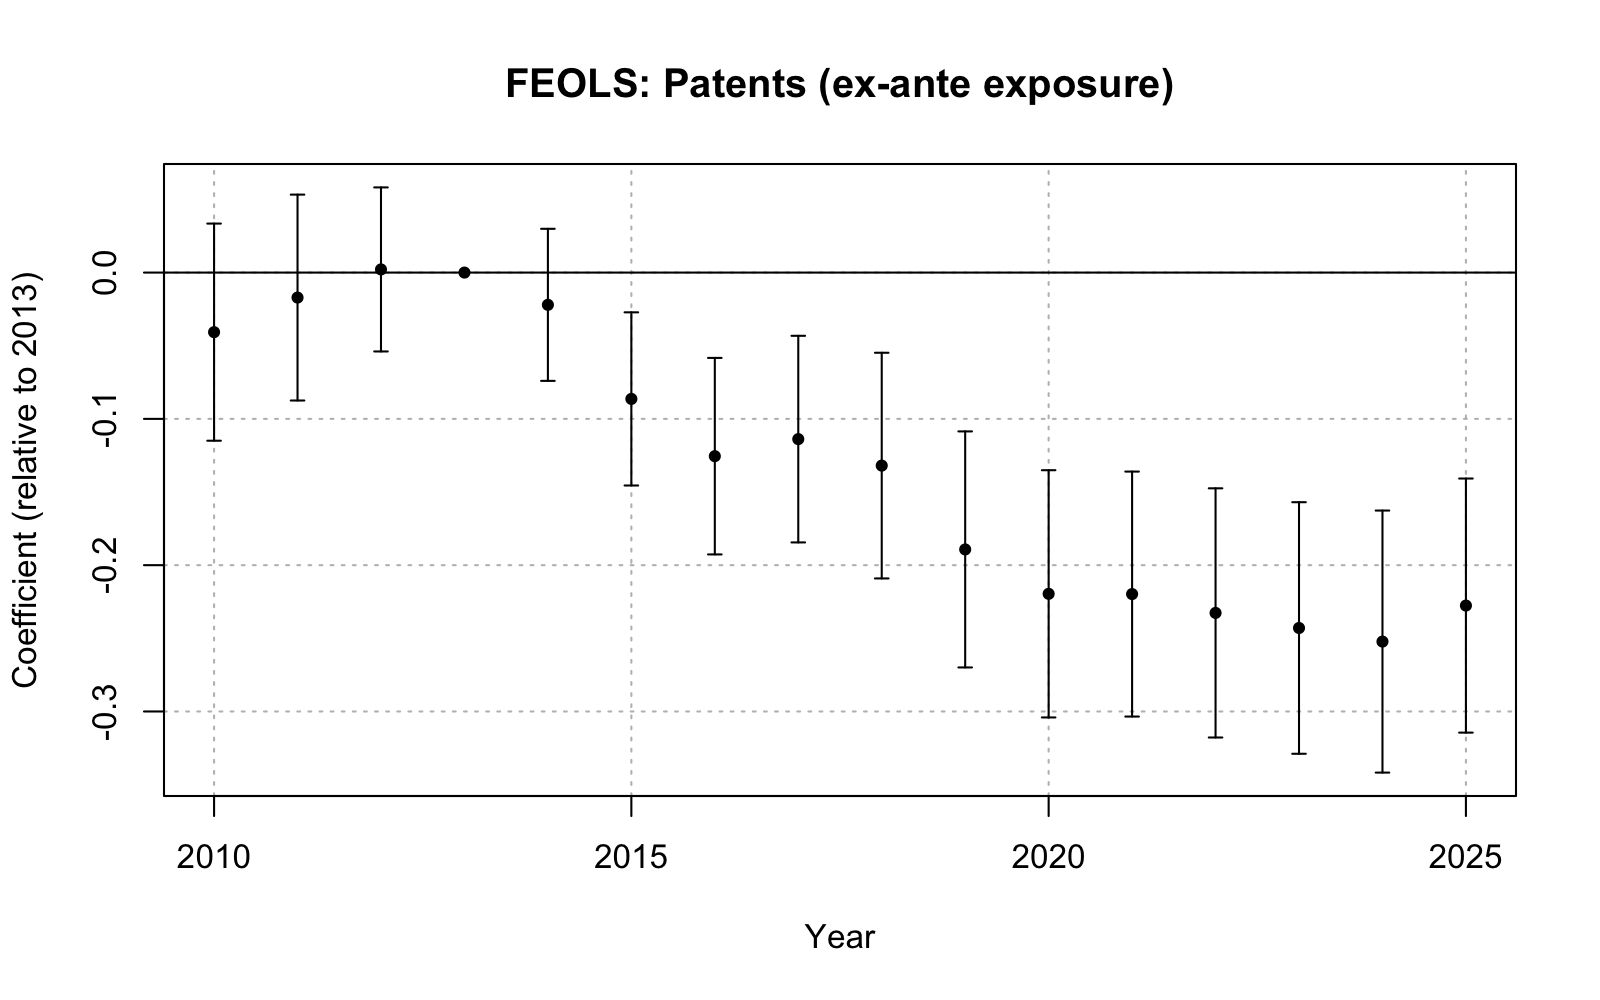
\includegraphics[width=\linewidth]{../output/RQ1/patent_feols_exante.png}
  \caption{FEOLS event study: patents, ex-ante Medicaid exposure}
  \label{fig:rq1_patent_feols_exante}
\end{figure}

\begin{figure}[!h]
  \centering
  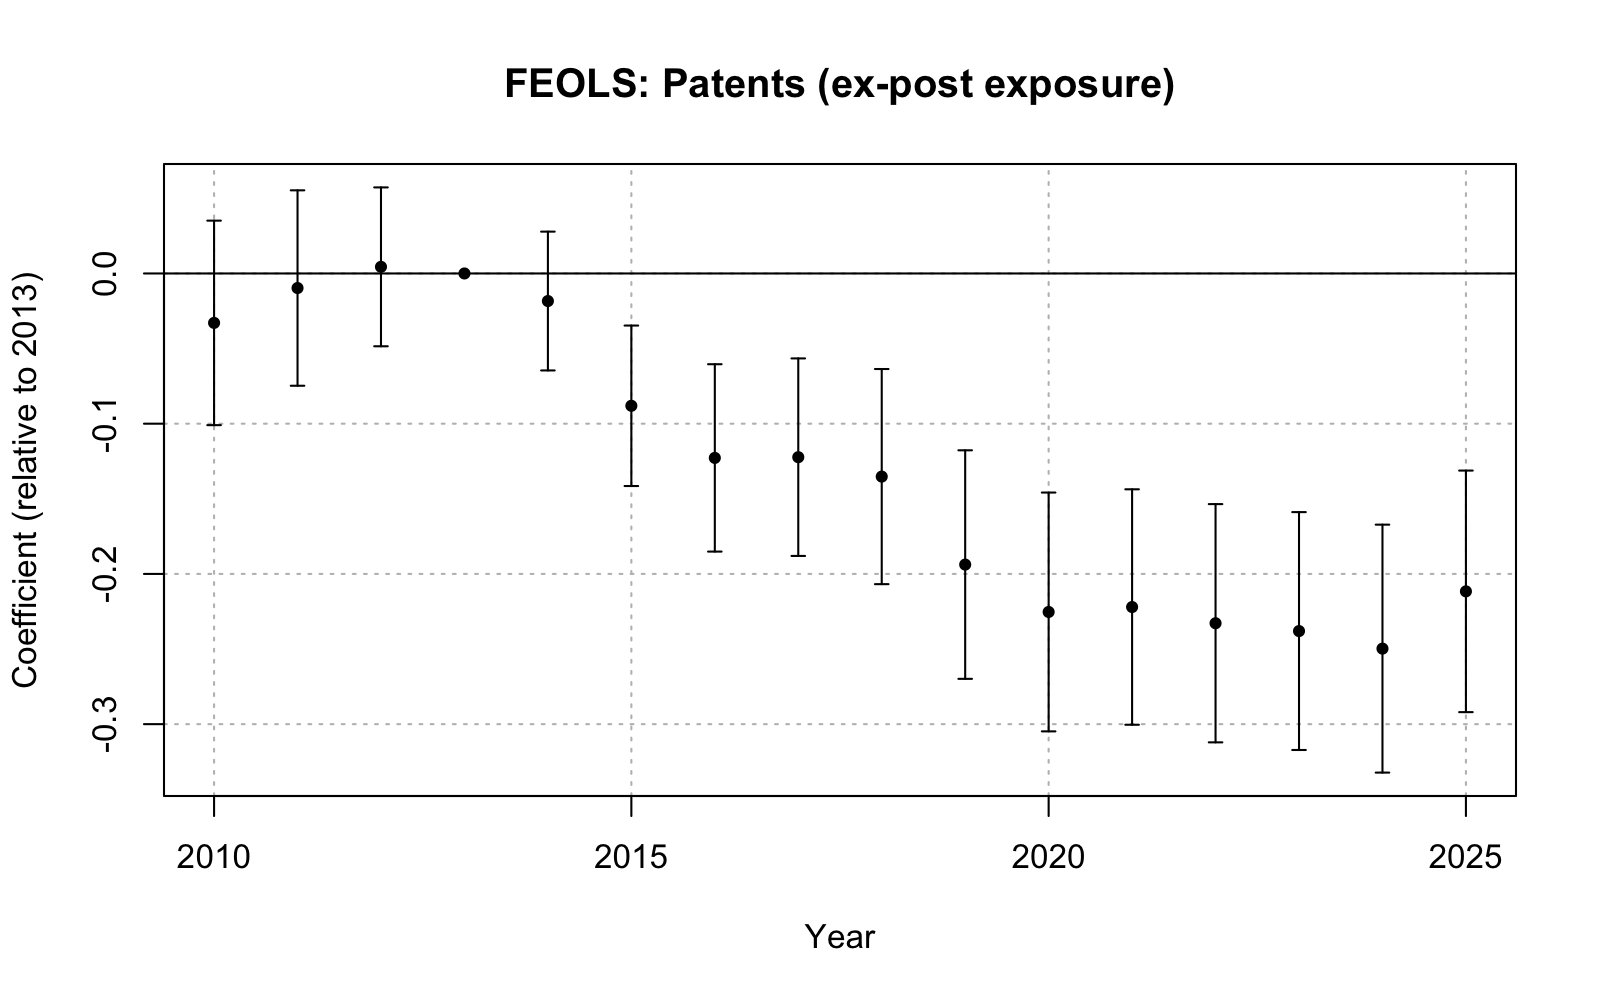
\includegraphics[width=\linewidth]{../output/RQ1/patent_feols_expost.png}
  \caption{FEOLS event study: patents, ex-post Medicaid exposure}
  \label{fig:rq1_patent_feols_expost}
\end{figure}

\begin{figure}[!h]
  \centering
  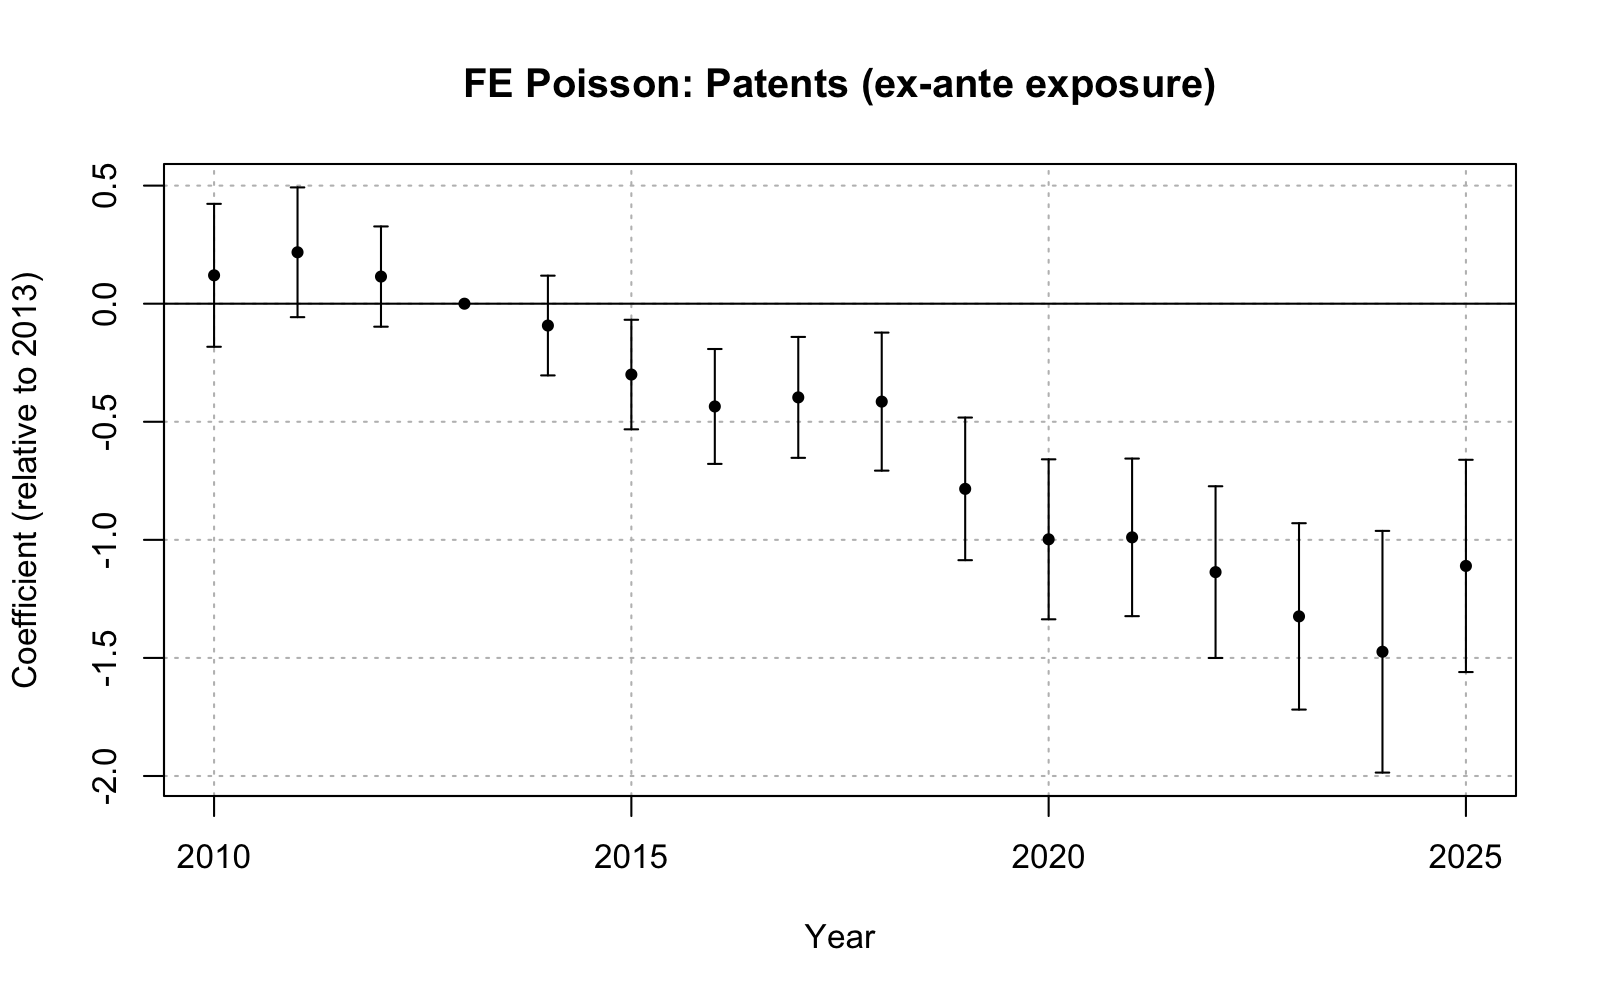
\includegraphics[width=\linewidth]{../output/RQ1/patent_poi_exante.png}
  \caption{FE Poisson event study: patents, ex-ante Medicaid exposure}
  \label{fig:rq1_patent_poi_exante}
\end{figure}

\begin{figure}[!h]
  \centering
  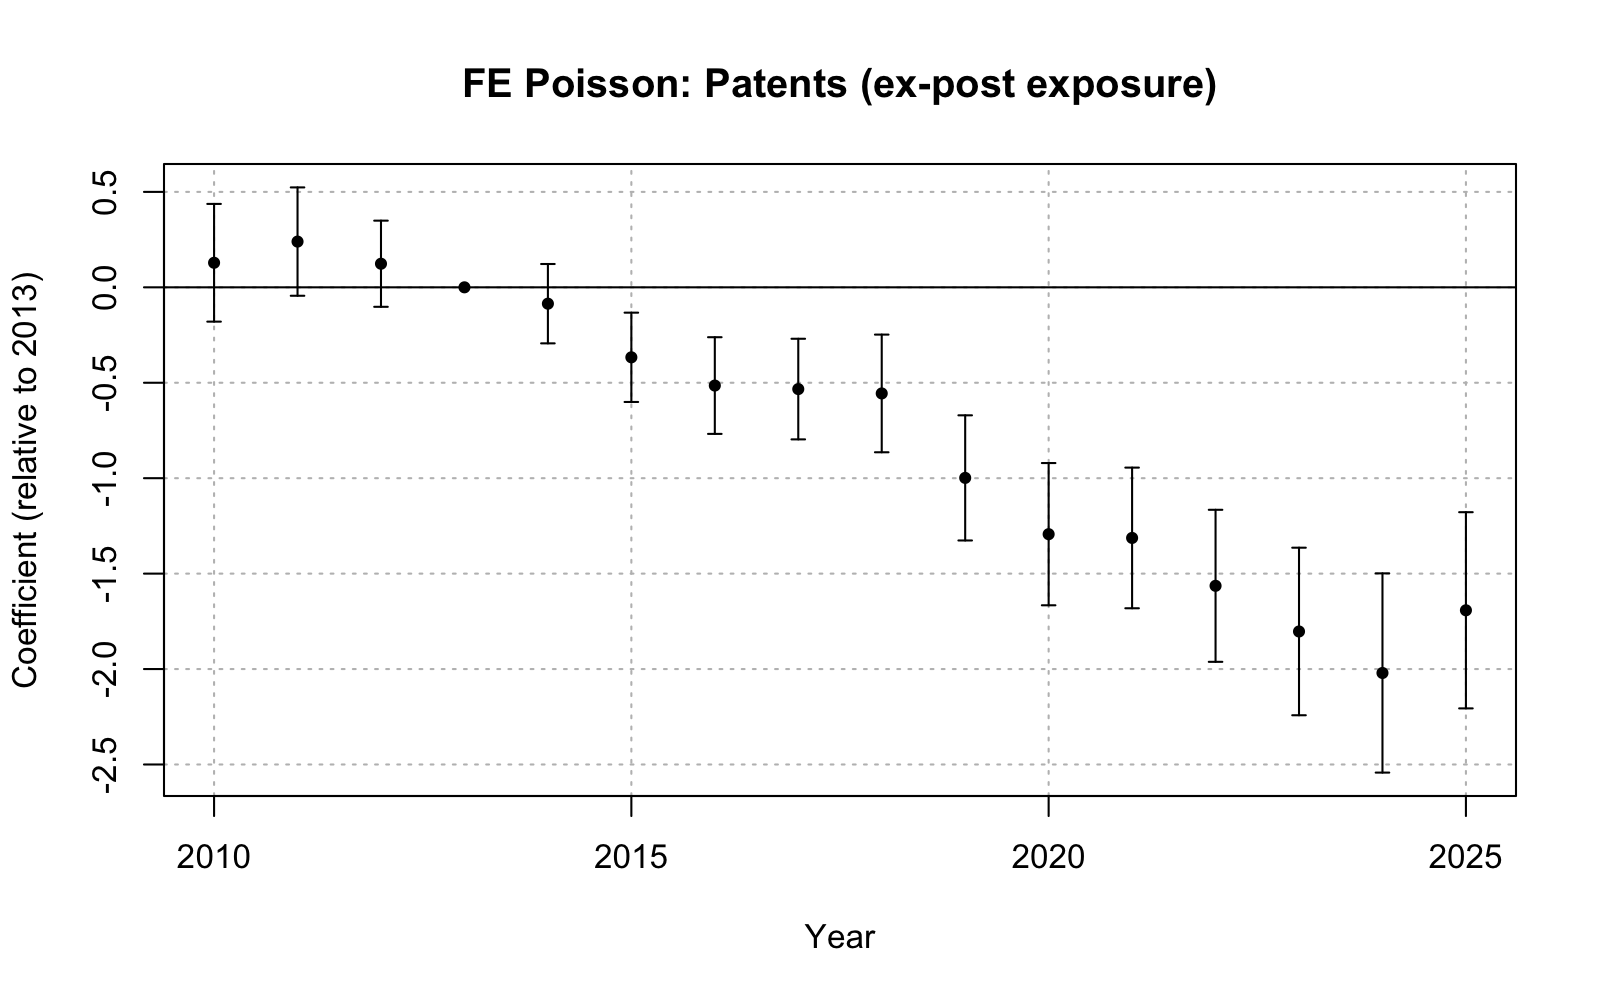
\includegraphics[width=\linewidth]{../output/RQ1/patent_poi_expost.png}
  \caption{FE Poisson event study: patents, ex-post Medicaid exposure}
  \label{fig:rq1_patent_poi_expost}
\end{figure}

\clearpage
\begingroup\footnotesize
\begin{table}
\centering
\begin{talltblr}[         %% tabularray outer open
entry=none,label=none,
note{}={* p \num{< 0.05}, ** p \num{< 0.01}, *** p \num{< 0.001}},
]                     %% tabularray outer close
{                     %% tabularray inner open
colspec={Q[]Q[]Q[]Q[]Q[]},
column{2,3,4,5}={}{halign=c,},
column{1}={}{halign=l,},
hline{32}={1,2,3,4,5}{solid, black, 0.05em},
}                     %% tabularray inner close
\toprule
& FEOLS: Ex Ante & FEOLS: Ex Post & FEPOIS: Ex Ante & FEPOIS: Ex Post \\ \midrule %% TinyTableHeader
2010 × medicaid\_market\_share & \num{-0.010}    & \num{-0.008}    & \num{0.120}     & \num{0.129}     \\
                                              & (\num{0.009})   & (\num{0.009})   & (\num{0.154})   & (\num{0.157})   \\
2011 × medicaid\_market\_share & \num{-0.004}    & \num{-0.002}    & \num{0.218}     & \num{0.240}     \\
                                              & (\num{0.009})   & (\num{0.008})   & (\num{0.140})   & (\num{0.145})   \\
2012 × medicaid\_market\_share & \num{0.001}     & \num{0.001}     & \num{0.115}     & \num{0.124}     \\
                                              & (\num{0.007})   & (\num{0.007})   & (\num{0.108})   & (\num{0.115})   \\
2014 × medicaid\_market\_share & \num{-0.006}    & \num{-0.005}    & \num{-0.092}    & \num{-0.086}    \\
                                              & (\num{0.007})   & (\num{0.006})   & (\num{0.108})   & (\num{0.106})   \\
2015 × medicaid\_market\_share & \num{-0.022}**  & \num{-0.022}**  & \num{-0.300}*   & \num{-0.367}**  \\
                                              & (\num{0.008})   & (\num{0.007})   & (\num{0.118})   & (\num{0.119})   \\
2016 × medicaid\_market\_share & \num{-0.031}*** & \num{-0.031}*** & \num{-0.435}*** & \num{-0.515}*** \\
                                              & (\num{0.009})   & (\num{0.008})   & (\num{0.124})   & (\num{0.129})   \\
2017 × medicaid\_market\_share & \num{-0.028}**  & \num{-0.031}*** & \num{-0.397}**  & \num{-0.533}*** \\
                                              & (\num{0.009})   & (\num{0.008})   & (\num{0.131})   & (\num{0.134})   \\
2018 × medicaid\_market\_share & \num{-0.033}*** & \num{-0.034}*** & \num{-0.415}**  & \num{-0.556}*** \\
                                              & (\num{0.010})   & (\num{0.009})   & (\num{0.149})   & (\num{0.157})   \\
2019 × medicaid\_market\_share & \num{-0.047}*** & \num{-0.048}*** & \num{-0.784}*** & \num{-0.998}*** \\
                                              & (\num{0.010})   & (\num{0.010})   & (\num{0.154})   & (\num{0.167})   \\
2020 × medicaid\_market\_share & \num{-0.055}*** & \num{-0.056}*** & \num{-0.998}*** & \num{-1.293}*** \\
                                              & (\num{0.011})   & (\num{0.010})   & (\num{0.173})   & (\num{0.190})   \\
2021 × medicaid\_market\_share & \num{-0.055}*** & \num{-0.056}*** & \num{-0.989}*** & \num{-1.313}*** \\
                                              & (\num{0.011})   & (\num{0.010})   & (\num{0.170})   & (\num{0.188})   \\
2022 × medicaid\_market\_share & \num{-0.058}*** & \num{-0.058}*** & \num{-1.137}*** & \num{-1.564}*** \\
                                              & (\num{0.011})   & (\num{0.010})   & (\num{0.186})   & (\num{0.203})   \\
2023 × medicaid\_market\_share & \num{-0.061}*** & \num{-0.060}*** & \num{-1.324}*** & \num{-1.803}*** \\
                                              & (\num{0.011})   & (\num{0.010})   & (\num{0.201})   & (\num{0.224})   \\
2024 × medicaid\_market\_share & \num{-0.063}*** & \num{-0.062}*** & \num{-1.474}*** & \num{-2.021}*** \\
                                              & (\num{0.011})   & (\num{0.011})   & (\num{0.261})   & (\num{0.266})   \\
2025 × medicaid\_market\_share & \num{-0.057}*** & \num{-0.053}*** & \num{-1.110}*** & \num{-1.692}*** \\
                                              & (\num{0.011})   & (\num{0.010})   & (\num{0.229})   & (\num{0.262})   \\
Num. obs.                                     & \num{21126784}  & \num{21126784}  & \num{5203776}   & \num{5203776}   \\
R2                                            & \num{0.392}     & \num{0.392}     &                 &                 \\
\bottomrule
\end{talltblr}
\end{table}

\endgroup

\clearpage

\subsection{FDA Approvals}

\begin{figure}[!h]
  \centering
  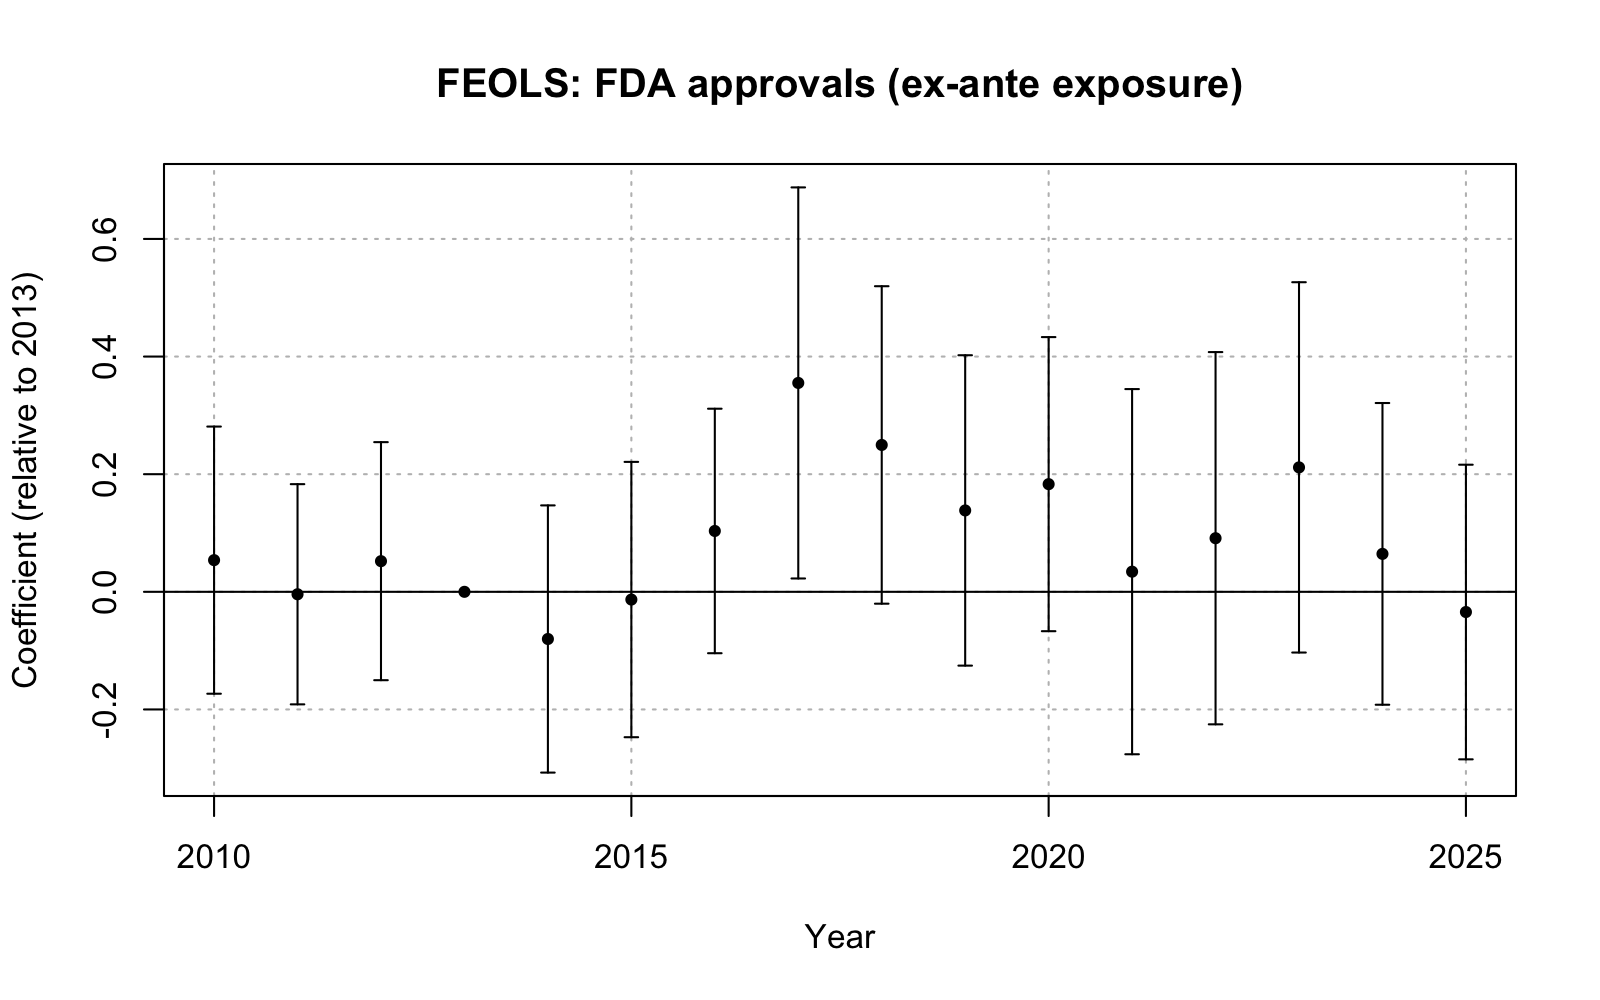
\includegraphics[width=\linewidth]{../output/RQ1/fda_feols_exante.png}
  \caption{FEOLS event study: FDA approvals, ex-ante Medicaid exposure}
  \label{fig:rq1_fda_feols_exante}
\end{figure}

\begin{figure}[!h]
  \centering
  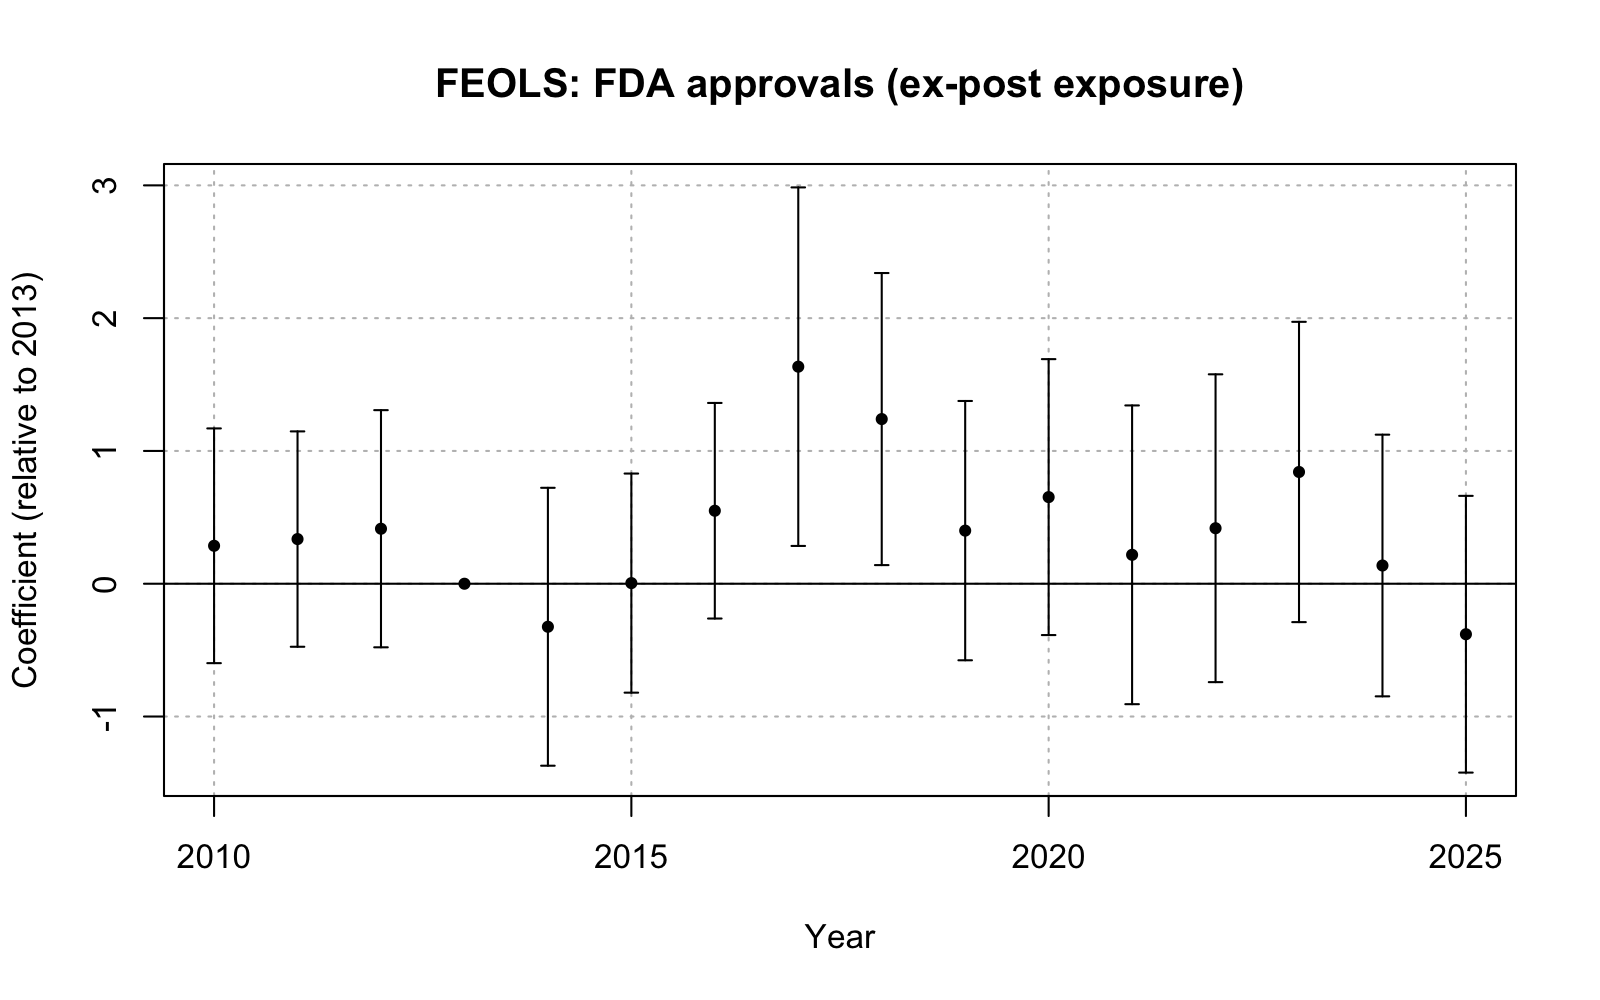
\includegraphics[width=\linewidth]{../output/RQ1/fda_feols_expost.png}
  \caption{FEOLS event study: FDA approvals, ex-post Medicaid exposure}
  \label{fig:rq1_fda_feols_expost}
\end{figure}

\begin{figure}[!h]
  \centering
  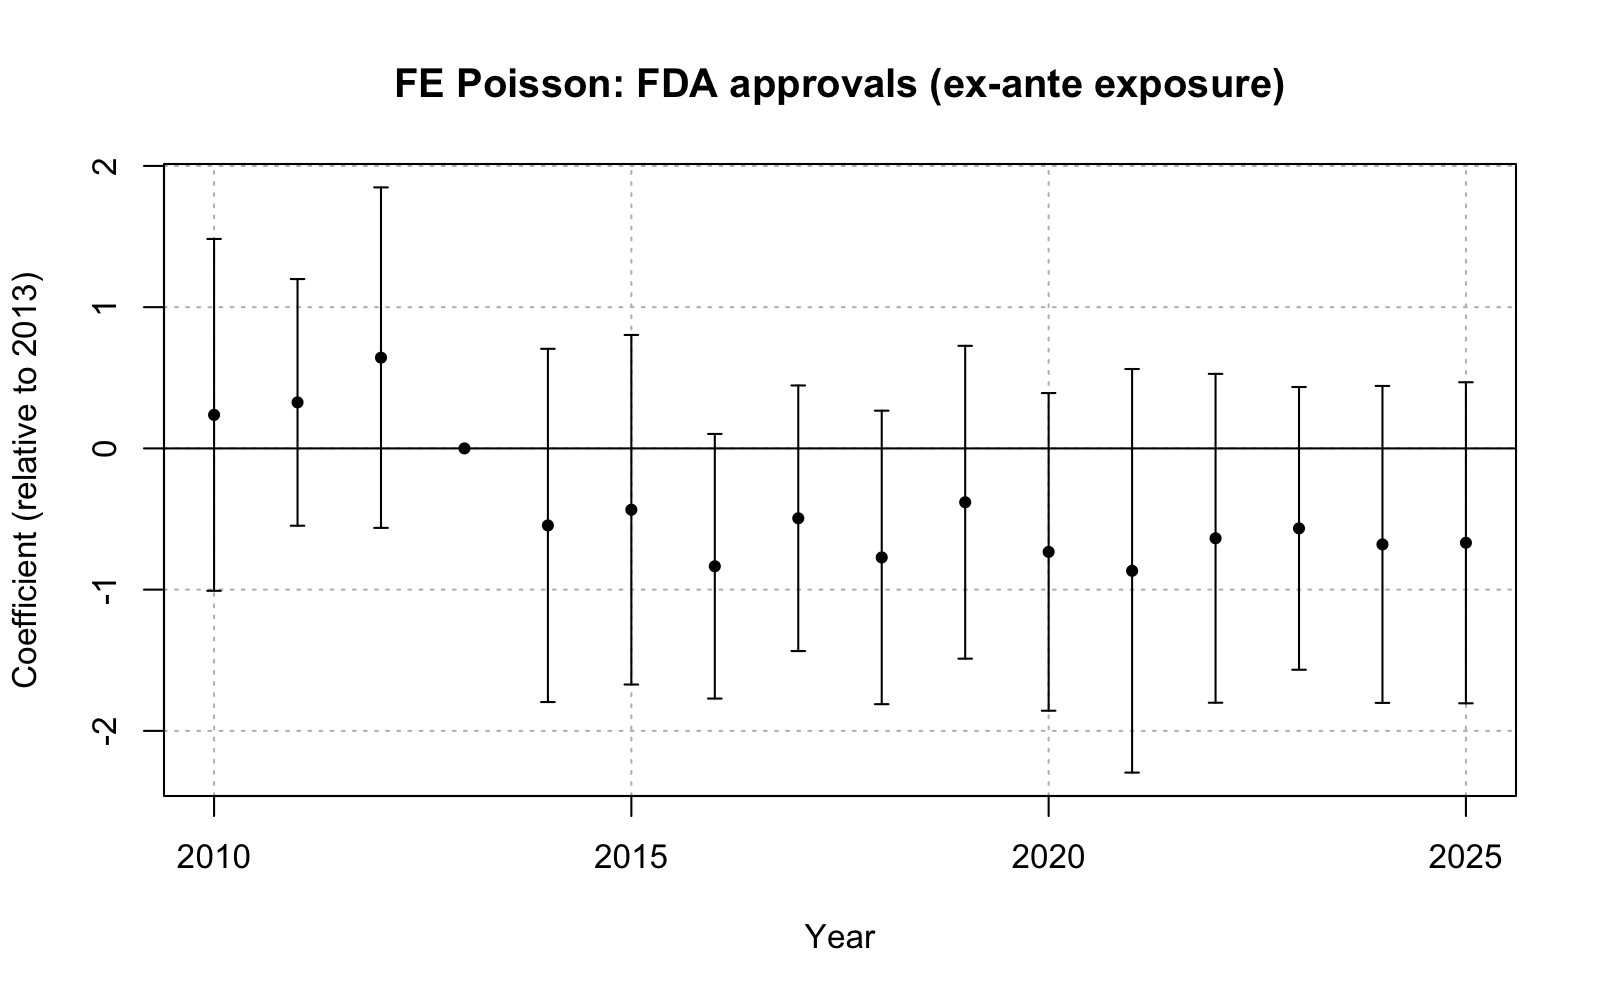
\includegraphics[width=\linewidth]{../output/RQ1/fda_poi_exante.png}
  \caption{FE Poisson event study: FDA approvals, ex-ante Medicaid exposure}
  \label{fig:rq1_fda_poi_exante}
\end{figure}

\begin{figure}[!h]
  \centering
  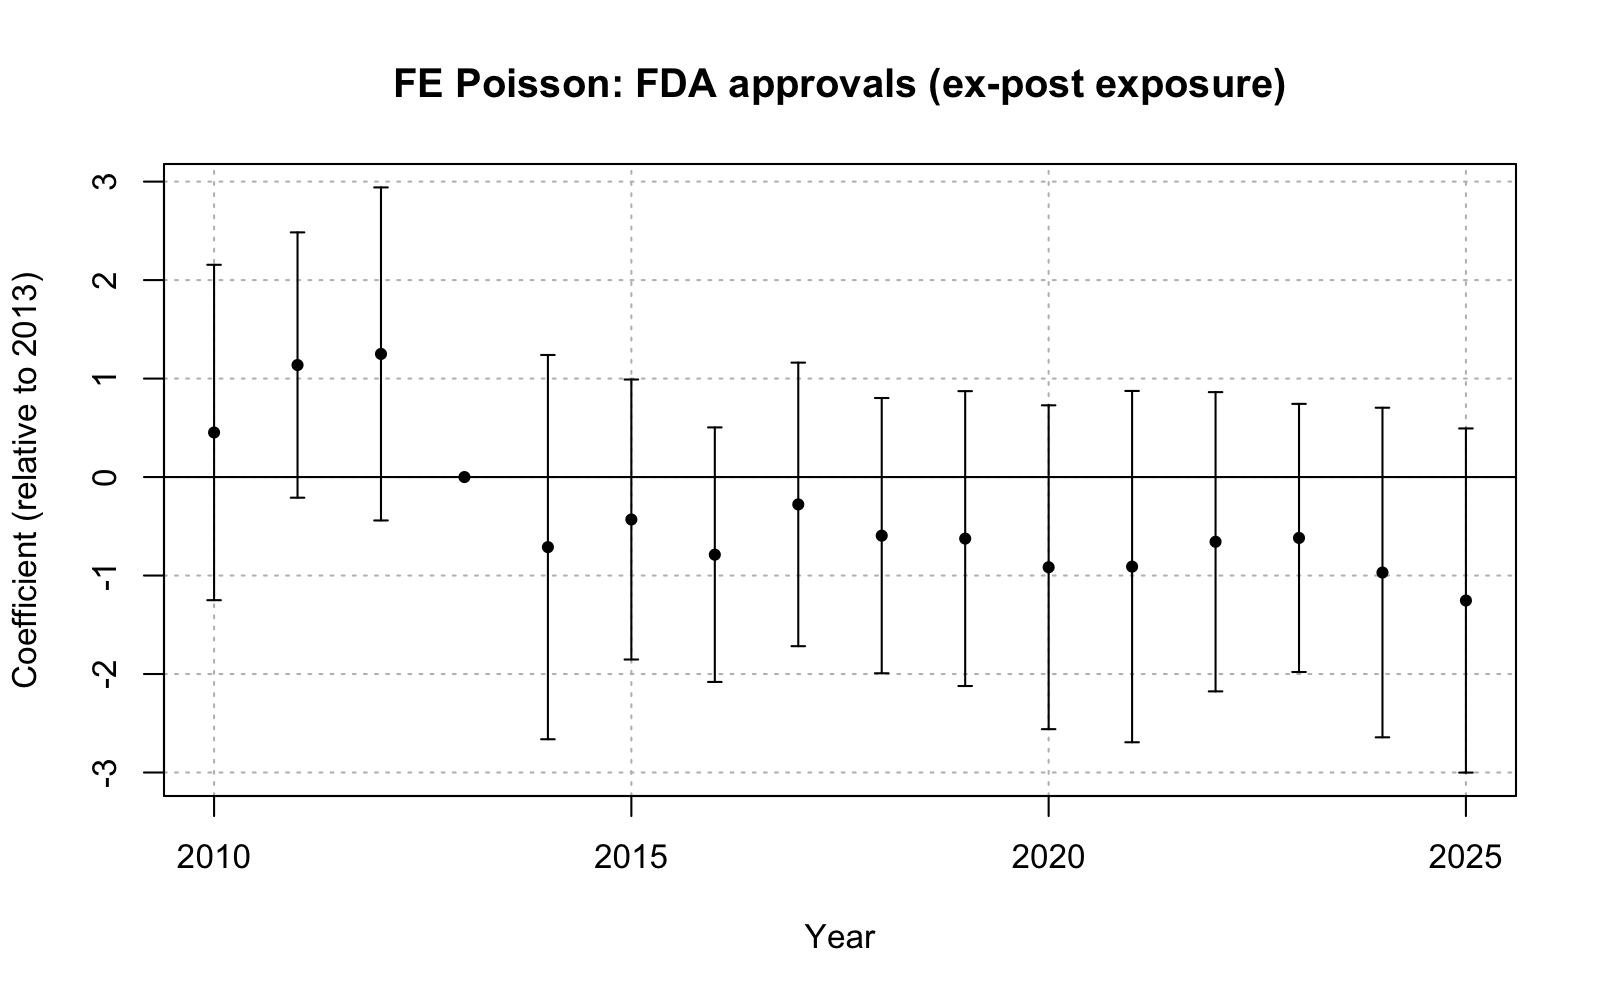
\includegraphics[width=\linewidth]{../output/RQ1/fda_poi_expost.png}
  \caption{FE Poisson event study: FDA approvals, ex-post Medicaid exposure}
  \label{fig:rq1_fda_poi_expost}
\end{figure}

\clearpage
\begingroup\footnotesize
\begin{table}
\centering
\begin{talltblr}[         %% tabularray outer open
entry=none,label=none,
note{}={* p \num{< 0.05}, ** p \num{< 0.01}, *** p \num{< 0.001}},
]                     %% tabularray outer close
{                     %% tabularray inner open
colspec={Q[]Q[]Q[]Q[]Q[]},
column{2,3,4,5}={}{halign=c,},
column{1}={}{halign=l,},
hline{32}={1,2,3,4,5}{solid, black, 0.05em},
}                     %% tabularray inner close
\toprule
& FEOLS: Ex Ante & FEOLS: Ex Post & FEPOIS: Ex Ante & FEPOIS: Ex Post \\ \midrule %% TinyTableHeader
2010 × medicaid\_market\_share & \num{0.054}   & \num{0.071}   & \num{0.237}   & \num{0.453}   \\
& (\num{0.116}) & (\num{0.113}) & (\num{0.636}) & (\num{0.869}) \\
2011 × medicaid\_market\_share & \num{-0.004}  & \num{0.084}   & \num{0.326}   & \num{1.138}   \\
& (\num{0.095}) & (\num{0.103}) & (\num{0.446}) & (\num{0.687}) \\
2012 × medicaid\_market\_share & \num{0.052}   & \num{0.104}   & \num{0.643}   & \num{1.250}   \\
& (\num{0.103}) & (\num{0.114}) & (\num{0.615}) & (\num{0.863}) \\
2014 × medicaid\_market\_share & \num{-0.080}  & \num{-0.081}  & \num{-0.545}  & \num{-0.711}  \\
& (\num{0.116}) & (\num{0.133}) & (\num{0.638}) & (\num{0.995}) \\
2015 × medicaid\_market\_share & \num{-0.013}  & \num{0.001}   & \num{-0.434}  & \num{-0.431}  \\
& (\num{0.119}) & (\num{0.105}) & (\num{0.631}) & (\num{0.725}) \\
2016 × medicaid\_market\_share & \num{0.103}   & \num{0.137}   & \num{-0.834}  & \num{-0.788}  \\
& (\num{0.106}) & (\num{0.103}) & (\num{0.478}) & (\num{0.659}) \\
2017 × medicaid\_market\_share & \num{0.355}*  & \num{0.409}*  & \num{-0.495}  & \num{-0.278}  \\
& (\num{0.169}) & (\num{0.172}) & (\num{0.480}) & (\num{0.735}) \\
2018 × medicaid\_market\_share & \num{0.250}   & \num{0.310}*  & \num{-0.772}  & \num{-0.595}  \\
& (\num{0.137}) & (\num{0.140}) & (\num{0.530}) & (\num{0.713}) \\
2019 × medicaid\_market\_share & \num{0.138}   & \num{0.100}   & \num{-0.381}  & \num{-0.625}  \\
& (\num{0.134}) & (\num{0.124}) & (\num{0.565}) & (\num{0.764}) \\
2020 × medicaid\_market\_share & \num{0.183}   & \num{0.163}   & \num{-0.733}  & \num{-0.916}  \\
& (\num{0.127}) & (\num{0.132}) & (\num{0.574}) & (\num{0.839}) \\
2021 × medicaid\_market\_share & \num{0.034}   & \num{0.054}   & \num{-0.867}  & \num{-0.909}  \\
& (\num{0.158}) & (\num{0.143}) & (\num{0.729}) & (\num{0.910}) \\
2022 × medicaid\_market\_share & \num{0.091}   & \num{0.104}   & \num{-0.637}  & \num{-0.657}  \\
& (\num{0.161}) & (\num{0.148}) & (\num{0.594}) & (\num{0.775}) \\
2023 × medicaid\_market\_share & \num{0.212}   & \num{0.210}   & \num{-0.566}  & \num{-0.618}  \\
& (\num{0.160}) & (\num{0.144}) & (\num{0.511}) & (\num{0.695}) \\
2024 × medicaid\_market\_share & \num{0.065}   & \num{0.034}   & \num{-0.680}  & \num{-0.969}  \\
& (\num{0.131}) & (\num{0.125}) & (\num{0.573}) & (\num{0.854}) \\
2025 × medicaid\_market\_share & \num{-0.034}  & \num{-0.095}  & \num{-0.668}  & \num{-1.254}  \\
& (\num{0.128}) & (\num{0.133}) & (\num{0.580}) & (\num{0.892}) \\
Num. obs.                                          & \num{604800}  & \num{604800}  & \num{168704}  & \num{168704}  \\
R2                                                 & \num{0.314}   & \num{0.314}   &                &                \\
\bottomrule
\end{talltblr}
\end{table}

\endgroup

\clearpage

% -----------------------------------------------------------------------
\section{RQ2: Medicaid Demand and PDL Exposure}
% -----------------------------------------------------------------------

\subsection{Patents}

\begin{figure}[!h]
  \centering
  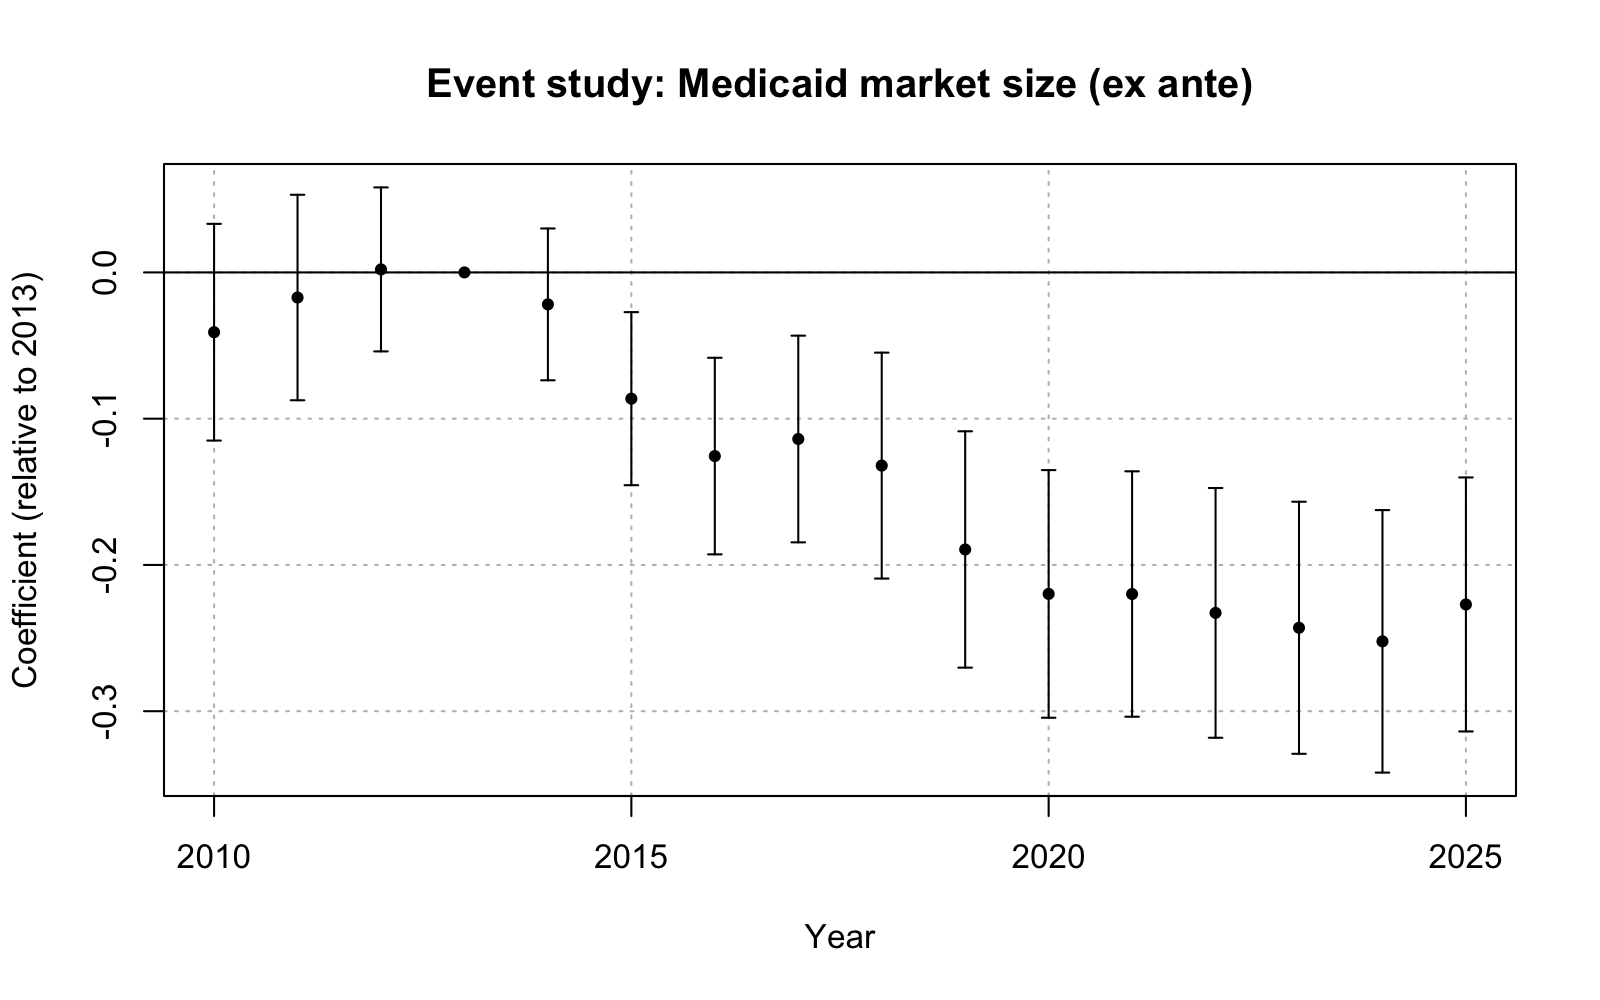
\includegraphics[width=\linewidth]{../output/RQ2/patent_feols_exante_medicaid.png}
  \caption{FEOLS event study: patents, Medicaid exposure (ex-ante)}
  \label{fig:rq2_patent_feols_exante_medicaid}
\end{figure}

\begin{figure}[!h]
  \centering
  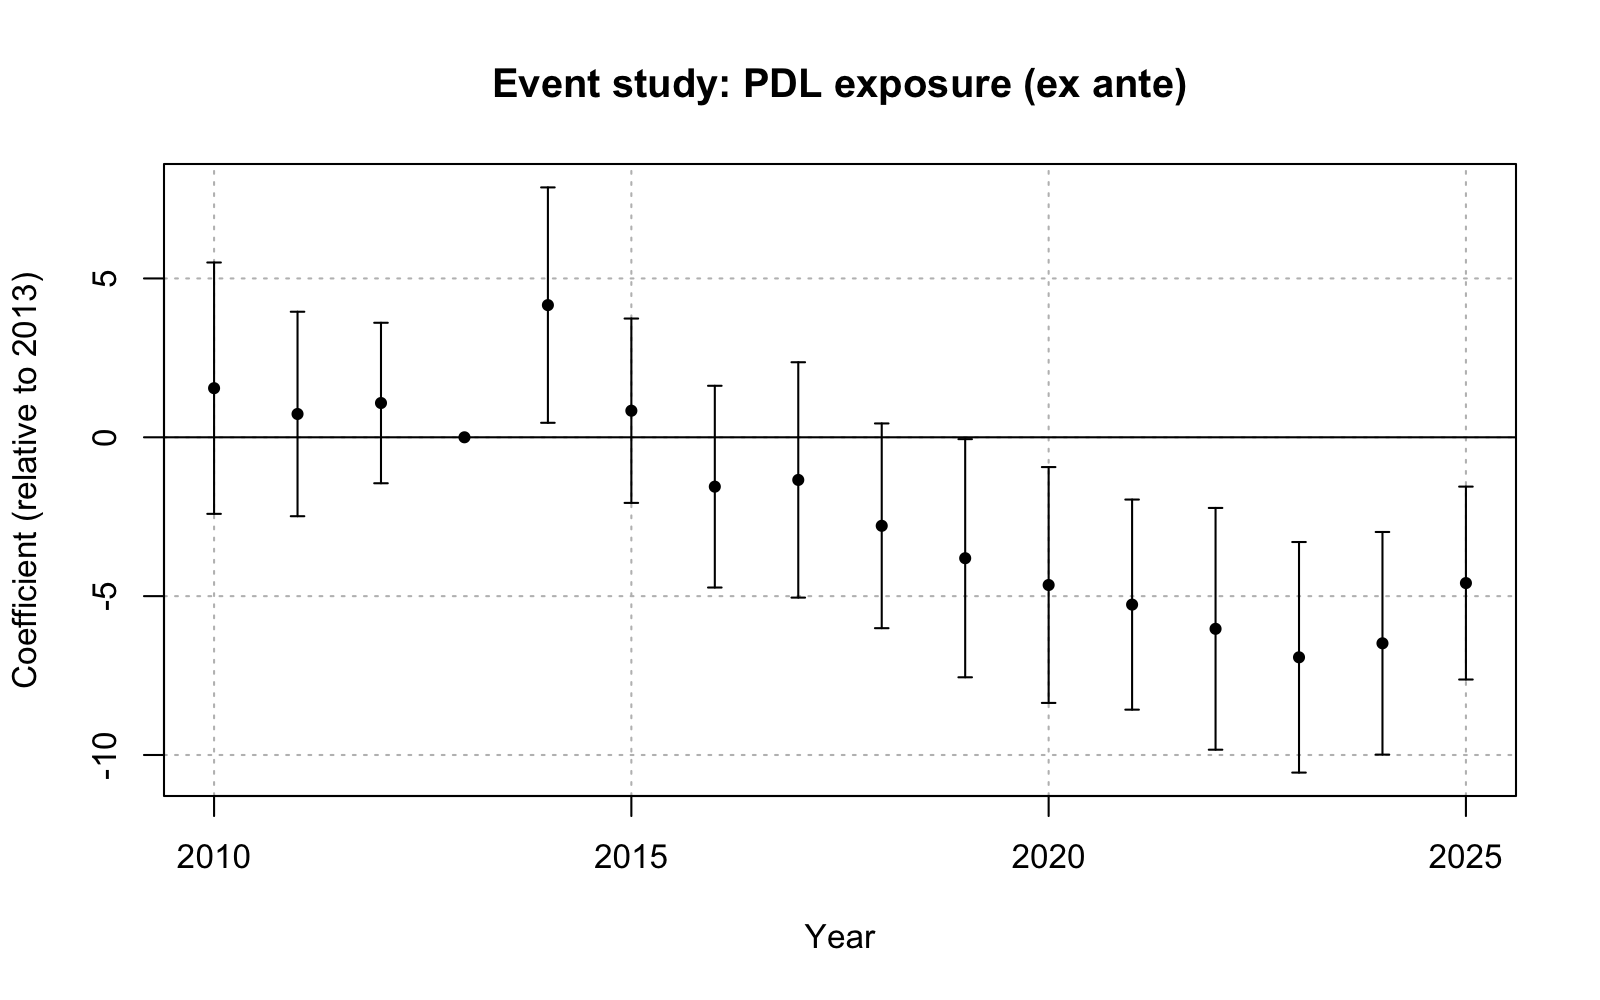
\includegraphics[width=\linewidth]{../output/RQ2/patent_feols_exante_pdl.png}
  \caption{FEOLS event study: patents, PDL exposure (ex-ante)}
  \label{fig:rq2_patent_feols_exante_pdl}
\end{figure}

\begin{figure}[!h]
  \centering
  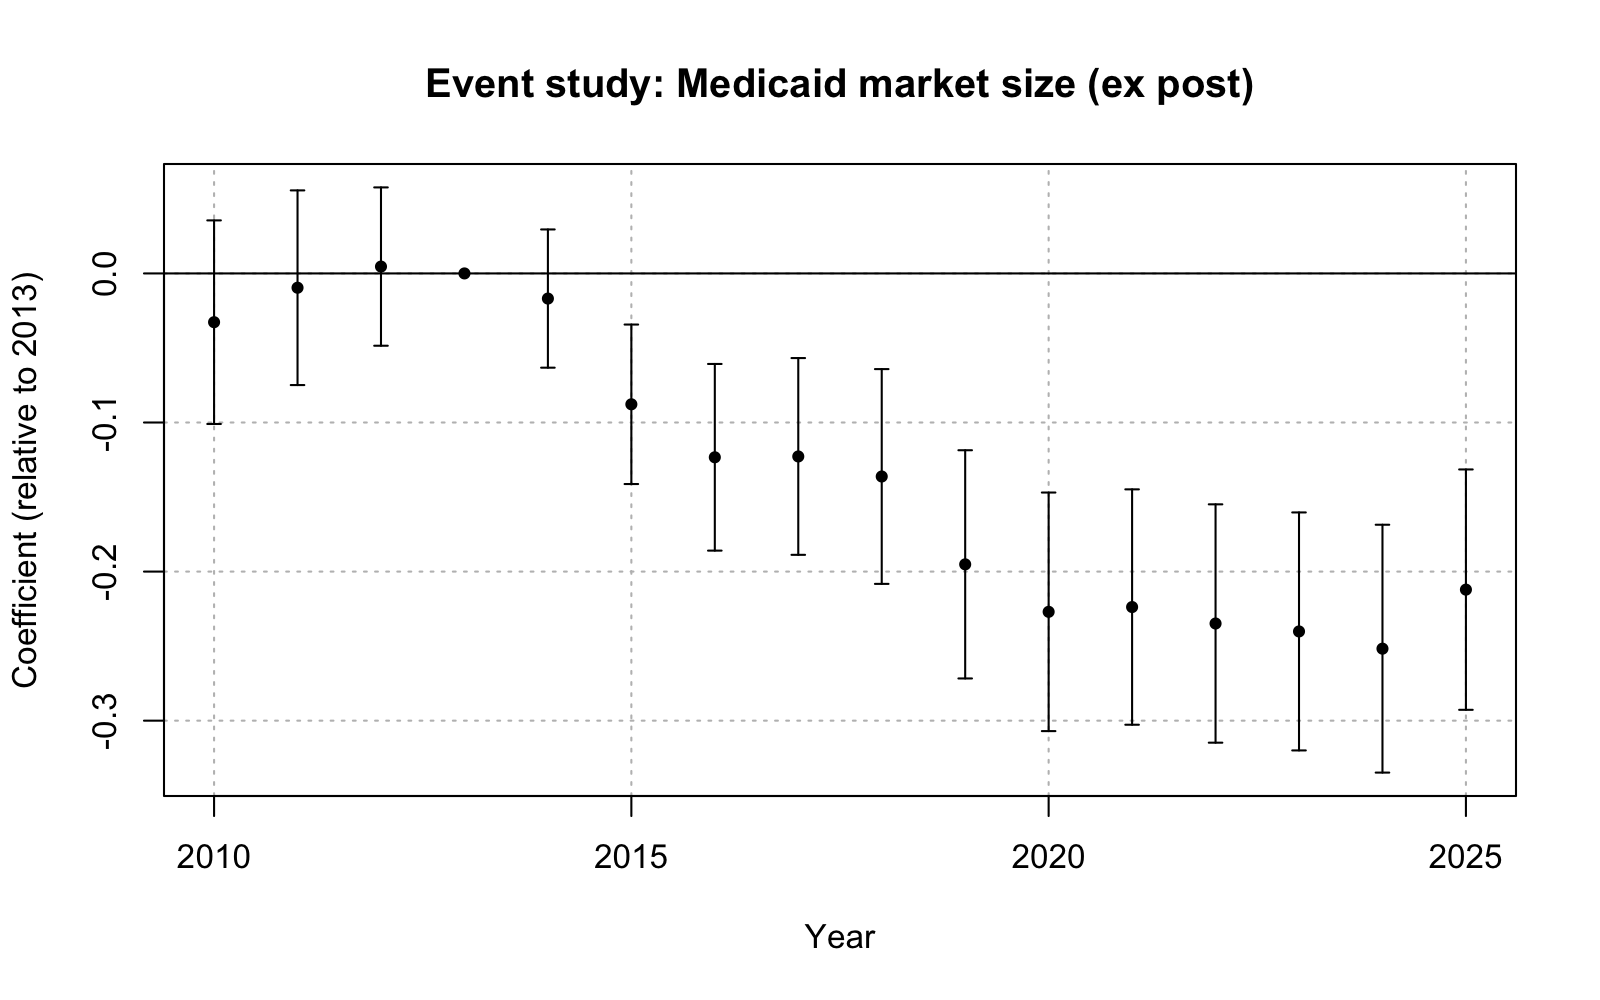
\includegraphics[width=\linewidth]{../output/RQ2/patent_feols_expost_medicaid.png}
  \caption{FEOLS event study: patents, Medicaid exposure (ex-post)}
  \label{fig:rq2_patent_feols_expost_medicaid}
\end{figure}

\begin{figure}[!h]
  \centering
  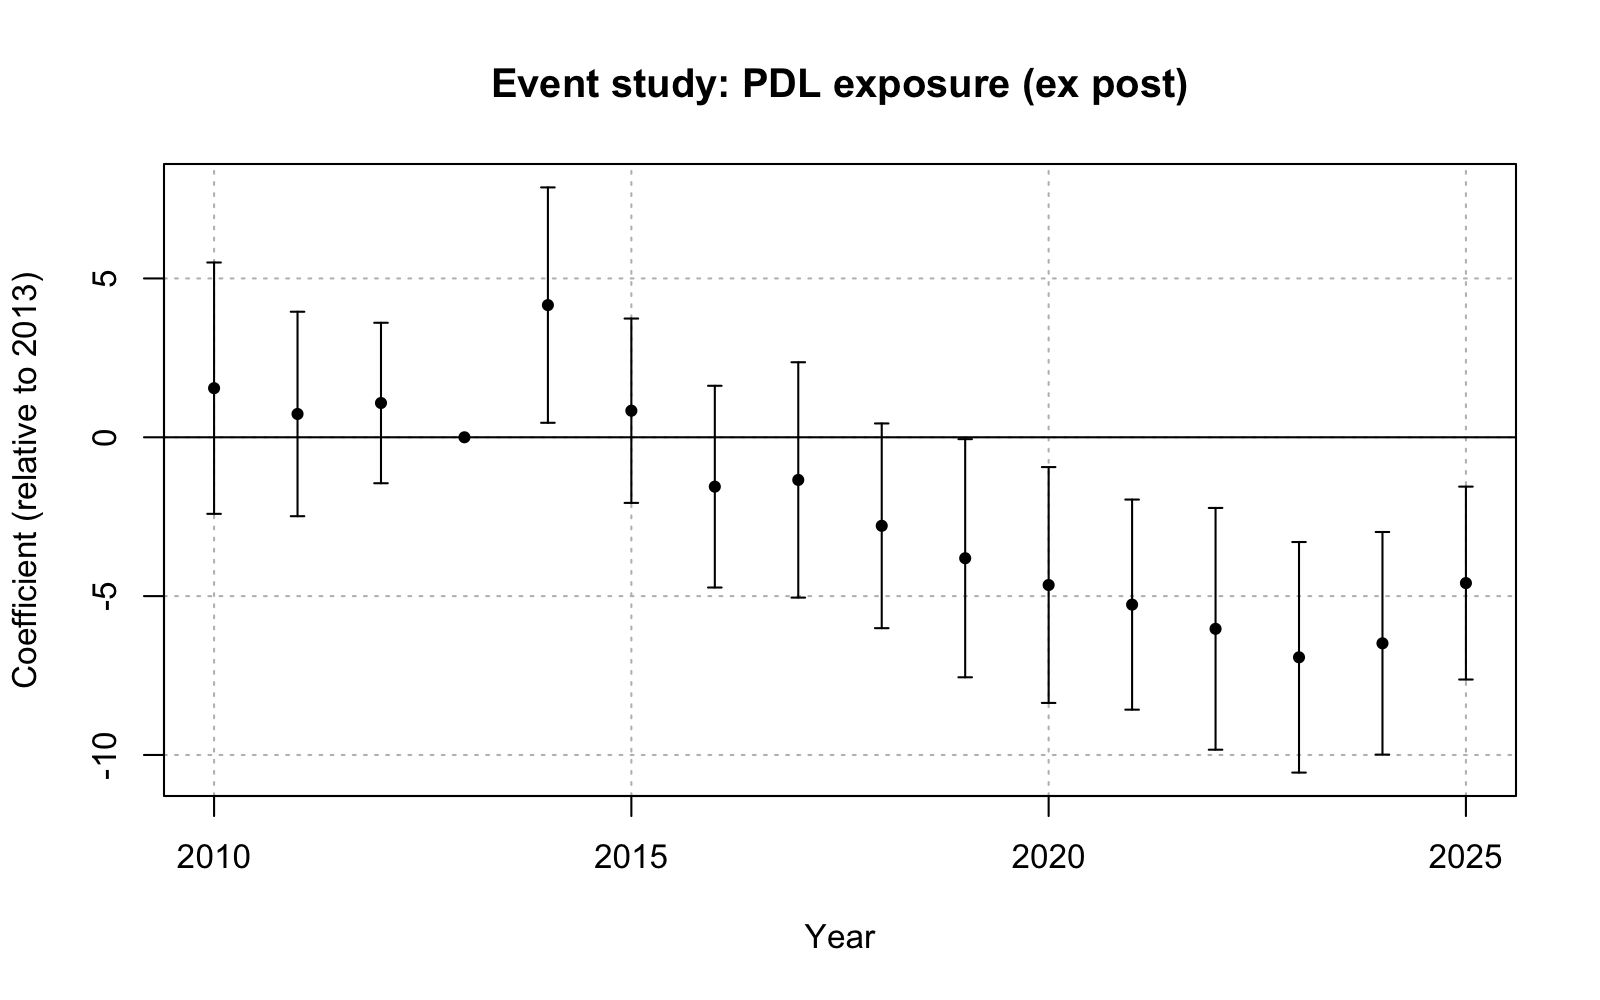
\includegraphics[width=\linewidth]{../output/RQ2/patent_feols_expost_pdl.png}
  \caption{FEOLS event study: patents, PDL exposure (ex-post)}
  \label{fig:rq2_patent_feols_expost_pdl}
\end{figure}

\clearpage
\begingroup\footnotesize
\begin{table}
\centering
\begin{talltblr}[         %% tabularray outer open
entry=none,label=none,
note{}={* p \num{< 0.05}, ** p \num{< 0.01}, *** p \num{< 0.001}},
]                     %% tabularray outer close
{                     %% tabularray inner open
colspec={Q[]Q[]Q[]},
column{2,3}={}{halign=c,},
column{1}={}{halign=l,},
hline{62}={1,2,3}{solid, black, 0.05em},
}                     %% tabularray inner close
\toprule
& FEOLS: Ex Ante & FEOLS: Ex Post \\ \midrule %% TinyTableHeader
2010 × medicaid\_market\_share & \num{-0.041}    & \num{-0.033}    \\
& (\num{0.038})   & (\num{0.035})   \\
2011 × medicaid\_market\_share & \num{-0.017}    & \num{-0.010}    \\
& (\num{0.036})   & (\num{0.033})   \\
2012 × medicaid\_market\_share & \num{0.002}     & \num{0.005}     \\
& (\num{0.029})   & (\num{0.027})   \\
2014 × medicaid\_market\_share & \num{-0.022}    & \num{-0.017}    \\
& (\num{0.026})   & (\num{0.024})   \\
2015 × medicaid\_market\_share & \num{-0.086}**  & \num{-0.088}**  \\
& (\num{0.030})   & (\num{0.027})   \\
2016 × medicaid\_market\_share & \num{-0.126}*** & \num{-0.123}*** \\
& (\num{0.034})   & (\num{0.032})   \\
2017 × medicaid\_market\_share & \num{-0.114}**  & \num{-0.123}*** \\
& (\num{0.036})   & (\num{0.034})   \\
2018 × medicaid\_market\_share & \num{-0.132}*** & \num{-0.136}*** \\
& (\num{0.039})   & (\num{0.037})   \\
2019 × medicaid\_market\_share & \num{-0.189}*** & \num{-0.195}*** \\
& (\num{0.041})   & (\num{0.039})   \\
2020 × medicaid\_market\_share & \num{-0.220}*** & \num{-0.227}*** \\
& (\num{0.043})   & (\num{0.041})   \\
2021 × medicaid\_market\_share & \num{-0.220}*** & \num{-0.224}*** \\
& (\num{0.043})   & (\num{0.040})   \\
2022 × medicaid\_market\_share & \num{-0.233}*** & \num{-0.235}*** \\
& (\num{0.044})   & (\num{0.041})   \\
2023 × medicaid\_market\_share & \num{-0.243}*** & \num{-0.240}*** \\
& (\num{0.044})   & (\num{0.041})   \\
2024 × medicaid\_market\_share & \num{-0.252}*** & \num{-0.252}*** \\
& (\num{0.046})   & (\num{0.042})   \\
2025 × medicaid\_market\_share & \num{-0.227}*** & \num{-0.212}*** \\
& (\num{0.044})   & (\num{0.041})   \\
2010 × in\_pdl                  & \num{1.546}     & \num{1.546}     \\
& (\num{2.018})   & (\num{2.018})   \\
2011 × in\_pdl                  & \num{0.734}     & \num{0.734}     \\
& (\num{1.642})   & (\num{1.642})   \\
2012 × in\_pdl                  & \num{1.079}     & \num{1.079}     \\
& (\num{1.289})   & (\num{1.289})   \\
2014 × in\_pdl                  & \num{4.161}*    & \num{4.161}*    \\
& (\num{1.890})   & (\num{1.890})   \\
2015 × in\_pdl                  & \num{0.836}     & \num{0.836}     \\
& (\num{1.480})   & (\num{1.480})   \\
2016 × in\_pdl                  & \num{-1.554}    & \num{-1.554}    \\
& (\num{1.620})   & (\num{1.620})   \\
2017 × in\_pdl                  & \num{-1.342}    & \num{-1.342}    \\
& (\num{1.890})   & (\num{1.890})   \\
2018 × in\_pdl                  & \num{-2.786}    & \num{-2.787}    \\
& (\num{1.644})   & (\num{1.644})   \\
2019 × in\_pdl                  & \num{-3.806}*   & \num{-3.807}*   \\
& (\num{1.912})   & (\num{1.912})   \\
2020 × in\_pdl                  & \num{-4.649}*   & \num{-4.650}*   \\
& (\num{1.894})   & (\num{1.894})   \\
2021 × in\_pdl                  & \num{-5.266}**  & \num{-5.267}**  \\
& (\num{1.687})   & (\num{1.687})   \\
2022 × in\_pdl                  & \num{-6.029}**  & \num{-6.029}**  \\
& (\num{1.941})   & (\num{1.941})   \\
2023 × in\_pdl                  & \num{-6.925}*** & \num{-6.926}*** \\
& (\num{1.851})   & (\num{1.851})   \\
2024 × in\_pdl                  & \num{-6.484}*** & \num{-6.485}*** \\
& (\num{1.788})   & (\num{1.788})   \\
2025 × in\_pdl                  & \num{-4.588}**  & \num{-4.589}**  \\
& (\num{1.549})   & (\num{1.549})   \\
Num. obs.                                        & \num{5281696}   & \num{5281696}   \\
R2                                               & \num{0.535}     & \num{0.535}     \\
\bottomrule
\end{talltblr}
\end{table}

\endgroup

\clearpage

\subsection{FDA Approvals}

\begin{figure}[!h]
  \centering
  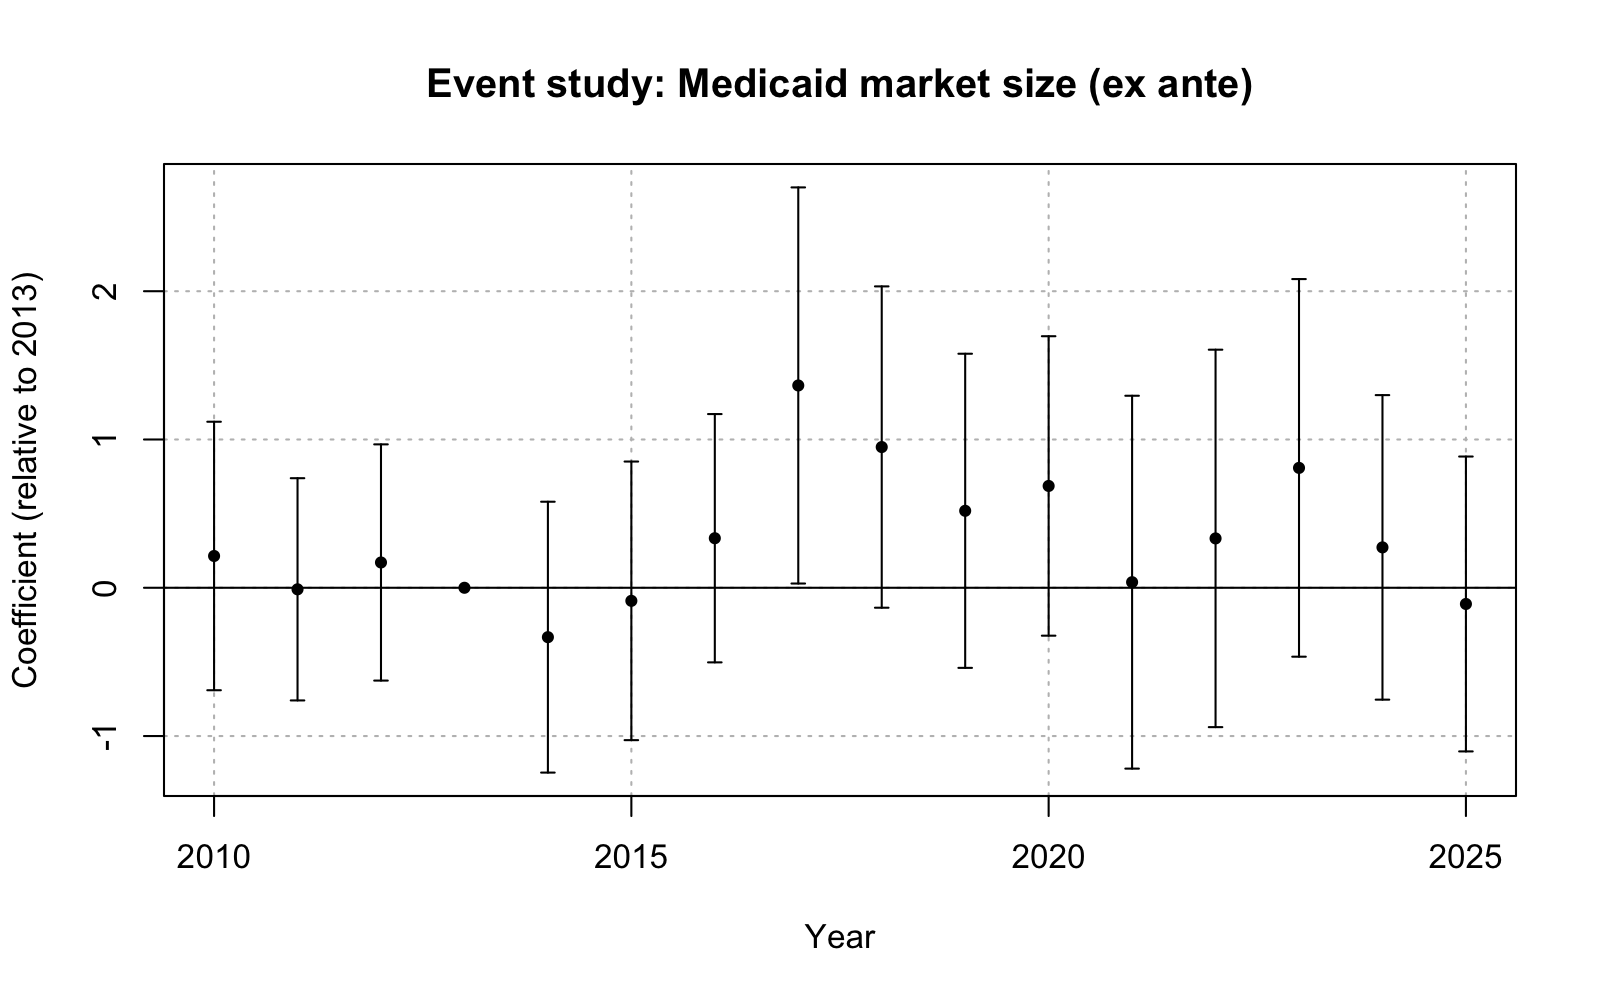
\includegraphics[width=\linewidth]{../output/RQ2/fda_feols_exante_medicaid.png}
  \caption{FEOLS event study: FDA approvals, Medicaid exposure (ex-ante)}
  \label{fig:rq2_fda_feols_exante_medicaid}
\end{figure}

\begin{figure}[!h]
  \centering
  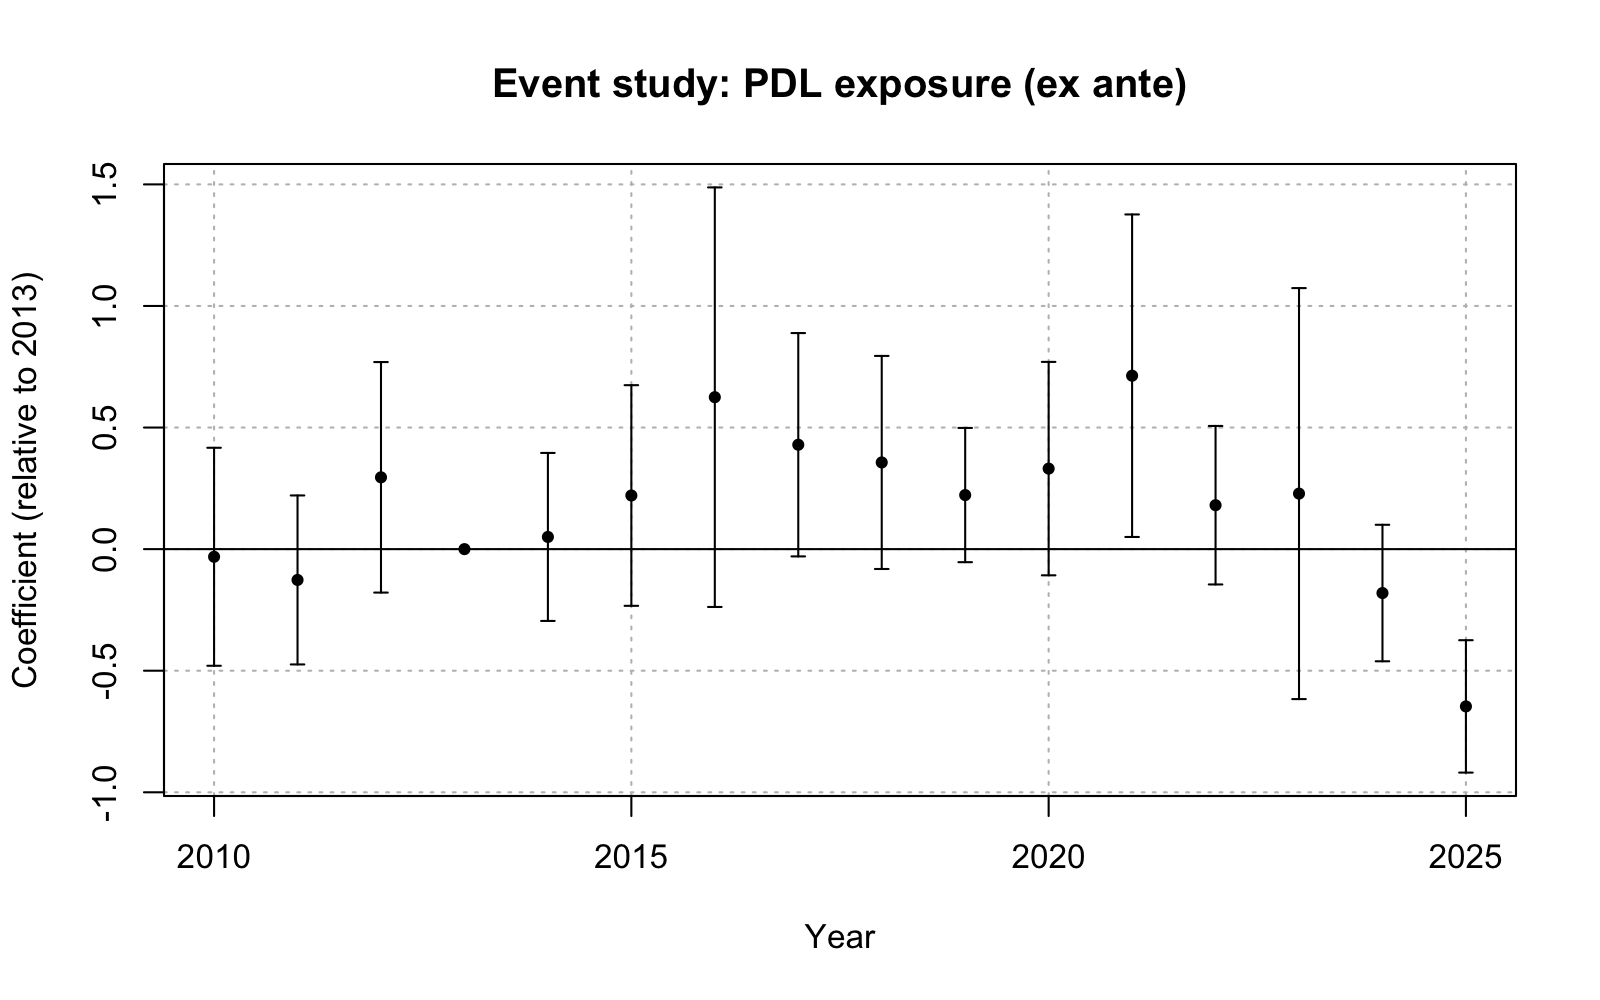
\includegraphics[width=\linewidth]{../output/RQ2/fda_feols_exante_pdl.png}
  \caption{FEOLS event study: FDA approvals, PDL exposure (ex-ante)}
  \label{fig:rq2_fda_feols_exante_pdl}
\end{figure}

\begin{figure}[!h]
  \centering
  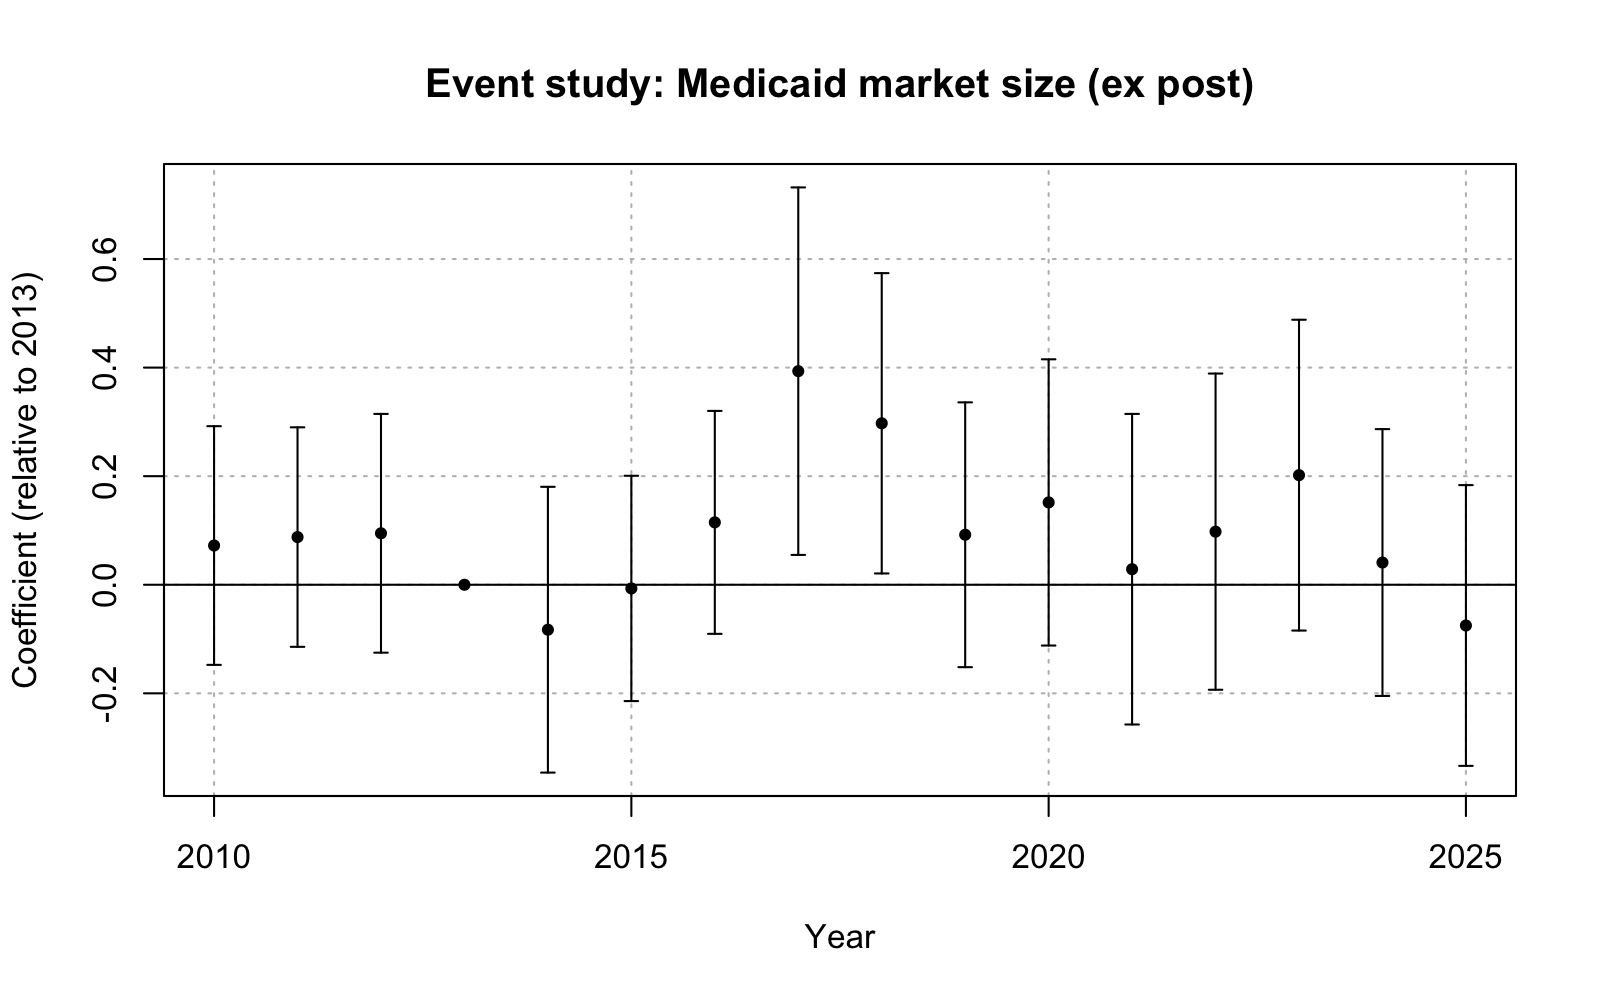
\includegraphics[width=\linewidth]{../output/RQ2/fda_feols_expost_medicaid.png}
  \caption{FEOLS event study: FDA approvals, Medicaid exposure (ex-post)}
  \label{fig:rq2_fda_feols_expost_medicaid}
\end{figure}

\begin{figure}[!h]
  \centering
  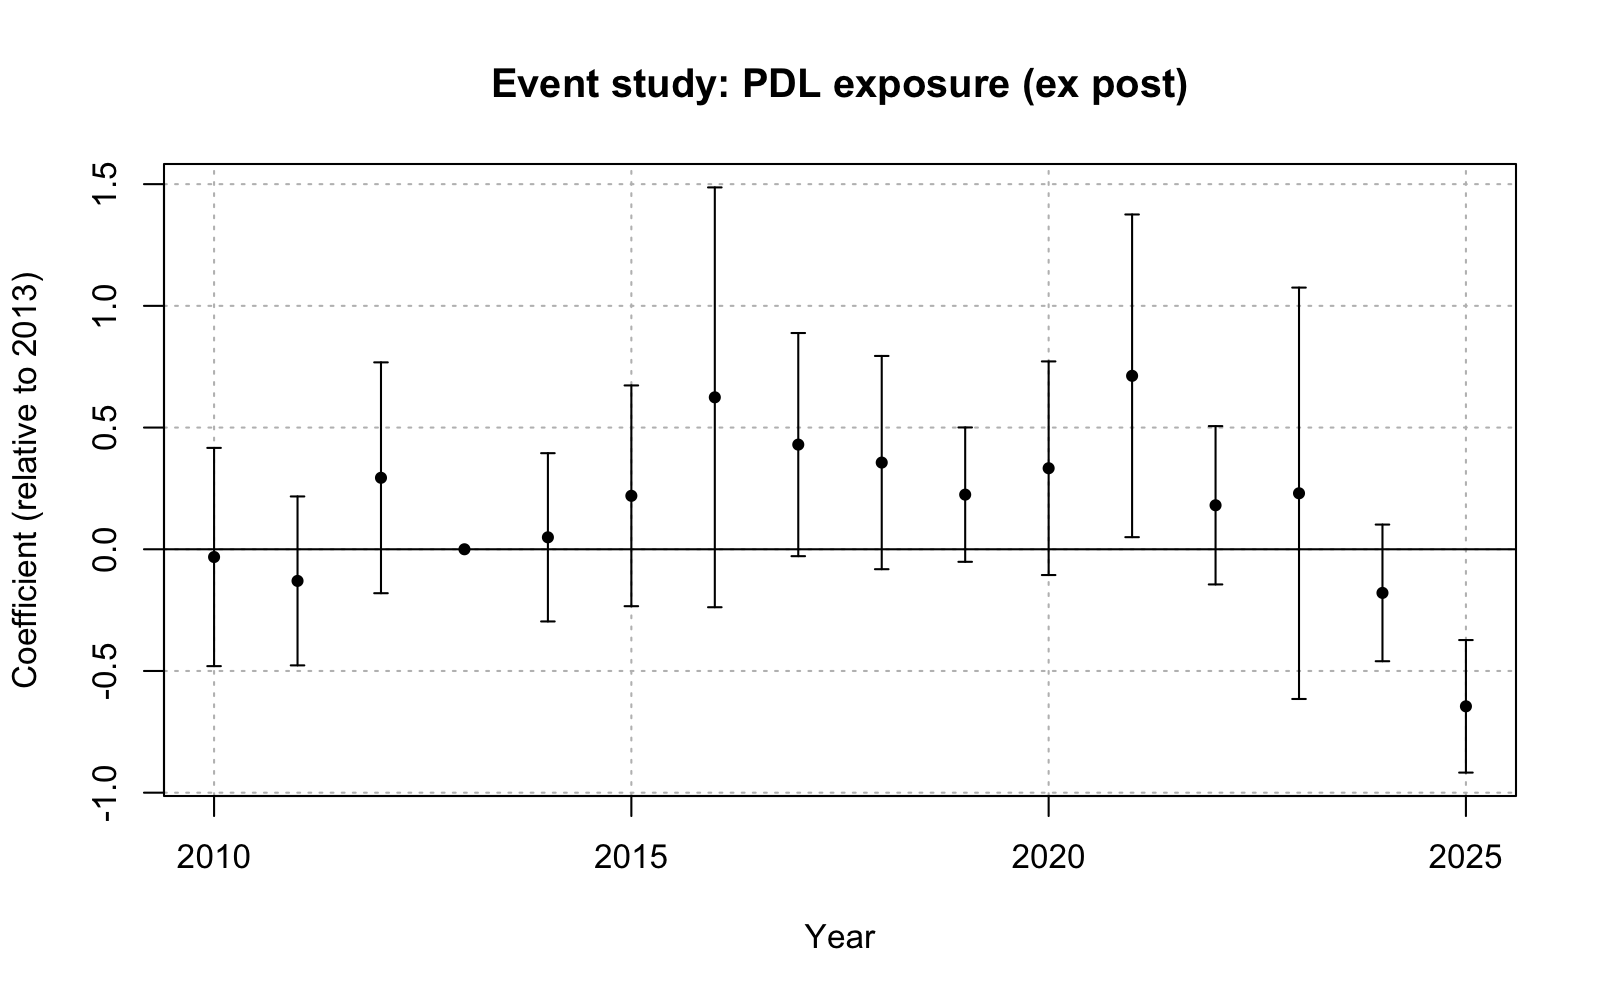
\includegraphics[width=\linewidth]{../output/RQ2/fda_feols_expost_pdl.png}
  \caption{FEOLS event study: FDA approvals, PDL exposure (ex-post)}
  \label{fig:rq2_fda_feols_expost_pdl}
\end{figure}

\clearpage
\begingroup\footnotesize
\begin{table}
\centering
\begin{talltblr}[         %% tabularray outer open
entry=none,label=none,
note{}={* p \num{< 0.05}, ** p \num{< 0.01}, *** p \num{< 0.001}},
]                     %% tabularray outer close
{                     %% tabularray inner open
width=\linewidth,
colspec={Q[]X[]X[]X[]X[]},
column{2,3,4,5}={}{halign=c,},
column{1}={}{halign=l,},
hline{33}={1,2,3,4,5}{solid, black, 0.05em},
}                     %% tabularray inner close
\toprule
& \SetCell[c=2]{c} FEOLS: Ex Ante && \SetCell[c=2]{c} FEOLS: Ex Post & \\
& Medicaid Share & PDL Exposure & Medicaid Share & PDL Exposure \\ \midrule
2010 & \num{0.214}   & \num{0.049}   & \num{0.285}   & \num{0.046}   \\
     & (\num{0.461}) & (\num{0.807}) & (\num{0.448}) & (\num{0.807}) \\
2011 & \num{-0.010}  & \num{-0.243}  & \num{0.344}   & \num{-0.257}  \\
     & (\num{0.382}) & (\num{0.712}) & (\num{0.412}) & (\num{0.711}) \\
2012 & \num{0.171}   & \num{1.402}   & \num{0.371}   & \num{1.395}   \\
     & (\num{0.406}) & (\num{0.911}) & (\num{0.447}) & (\num{0.912}) \\
2014 & \num{-0.333}  & \num{0.403}   & \num{-0.338}  & \num{0.398}   \\
     & (\num{0.465}) & (\num{0.647}) & (\num{0.536}) & (\num{0.647}) \\
2015 & \num{-0.088}  & \num{1.163}   & \num{-0.037}  & \num{1.158}   \\
     & (\num{0.478}) & (\num{0.881}) & (\num{0.422}) & (\num{0.881}) \\
2016 & \num{0.334}   & \num{2.645}   & \num{0.456}   & \num{2.642}   \\
     & (\num{0.426}) & (\num{1.683}) & (\num{0.418}) & (\num{1.682}) \\
2017 & \num{1.364}*  & \num{1.923}   & \num{1.566}*  & \num{1.924}   \\
     & (\num{0.680}) & (\num{0.994}) & (\num{0.690}) & (\num{0.992}) \\
2018 & \num{0.949}   & \num{1.684}   & \num{1.181}*  & \num{1.683}   \\
     & (\num{0.552}) & (\num{1.021}) & (\num{0.563}) & (\num{1.021}) \\
2019 & \num{0.519}   & \num{1.164}*  & \num{0.359}   & \num{1.171}*  \\
     & (\num{0.539}) & (\num{0.592}) & (\num{0.498}) & (\num{0.591}) \\
2020 & \num{0.687}   & \num{1.579}   & \num{0.598}   & \num{1.585}   \\
     & (\num{0.514}) & (\num{0.942}) & (\num{0.537}) & (\num{0.942}) \\
2021 & \num{0.038}   & \num{3.114}*  & \num{0.103}   & \num{3.110}*  \\
     & (\num{0.640}) & (\num{1.394}) & (\num{0.583}) & (\num{1.393}) \\
2022 & \num{0.333}   & \num{0.994}   & \num{0.381}   & \num{0.994}   \\
     & (\num{0.648}) & (\num{0.655}) & (\num{0.593}) & (\num{0.653}) \\
2023 & \num{0.809}   & \num{1.185}   & \num{0.798}   & \num{1.191}   \\
     & (\num{0.649}) & (\num{1.738}) & (\num{0.583}) & (\num{1.737}) \\
2024 & \num{0.272}   & \num{-0.452}  & \num{0.154}   & \num{-0.447}  \\
     & (\num{0.523}) & (\num{0.590}) & (\num{0.501}) & (\num{0.589}) \\
2025 & \num{-0.109}  & \num{-1.118}  & \num{-0.347}  & \num{-1.113}  \\
     & (\num{0.506}) & (\num{0.908}) & (\num{0.525}) & (\num{0.908}) \\
Num. obs. & \num{151200} & & \num{151200} & \\
R2        & \num{0.609}  & & \num{0.609}  & \\
\bottomrule
\end{talltblr}
\end{table}

\endgroup

\clearpage

% -----------------------------------------------------------------------
\section{RQ3: Therapeutic-Class Heterogeneity}
% -----------------------------------------------------------------------

\subsection{Patents}

\begin{center}
\begingroup\footnotesize
\begin{table}
\centering
\begin{talltblr}[         %% tabularray outer open
entry=none,label=none,
note{}={* p \num{< 0.05}, ** p \num{< 0.01}, *** p \num{< 0.001}},
]                     %% tabularray outer close
{                     %% tabularray inner open
colspec={Q[]Q[]Q[]},
column{2,3}={}{halign=c,},
column{1}={}{halign=l,},
hline{26}={1,2,3}{solid, black, 0.05em},
}                     %% tabularray inner close
\toprule
& FEOLS: Ex Ante & FEOLS: Ex Post \\ \midrule
Medicaid Share × ATC = A & \num{-0.165}*** & \num{-0.157}*** \\
& (\num{0.033})   & (\num{0.031})   \\
Medicaid Share × ATC = B & \num{0.134}***  & \num{0.151}***  \\
& (\num{0.024})   & (\num{0.027})   \\
Medicaid Share × ATC = C & \num{-0.123}*** & \num{-0.094}*** \\
& (\num{0.019})   & (\num{0.015})   \\
Medicaid Share × ATC = D & \num{-0.030}    & \num{-0.017}    \\
& (\num{0.108})   & (\num{0.062})   \\
Medicaid Share × ATC = G & \num{0.037}     & \num{0.032}     \\
& (\num{0.056})   & (\num{0.049})   \\
Medicaid Share × ATC = H & \num{0.876}***  & \num{0.619}***  \\
& (\num{0.136})   & (\num{0.096})   \\
Medicaid Share × ATC = J & \num{0.055}     & \num{0.035}     \\
& (\num{0.054})   & (\num{0.034})   \\
Medicaid Share × ATC = L & \num{0.346}     & \num{0.443}     \\
& (\num{0.452})   & (\num{0.578})   \\
Medicaid Share × ATC = M & \num{-0.336}*** & \num{-0.212}*** \\
& (\num{0.076})   & (\num{0.048})   \\
Medicaid Share × ATC = N & \num{-0.125}*** & \num{-0.174}*** \\
& (\num{0.028})   & (\num{0.039})   \\
Medicaid Share × ATC = R & \num{0.005}     & \num{0.005}     \\
& (\num{0.003})   & (\num{0.003})   \\
Medicaid Share × ATC = S & \num{0.093}***  & \num{0.105}***  \\
& (\num{0.017})   & (\num{0.020})   \\
Num. obs.                & \num{19617728}  & \num{19617728}  \\
R2                       & \num{0.247}     & \num{0.247}     \\
\bottomrule
\end{talltblr}
\end{table}

\endgroup
\end{center}

\subsection{FDA Approvals}

\begin{center}
\begingroup\footnotesize
\begin{table}
\centering
\begin{talltblr}[         %% tabularray outer open
entry=none,label=none,
note{}={* p \num{< 0.05}, ** p \num{< 0.01}, *** p \num{< 0.001}},
]                     %% tabularray outer close
{                     %% tabularray inner open
colspec={Q[]Q[]Q[]},
column{2,3}={}{halign=c,},
column{1}={}{halign=l,},
hline{26}={1,2,3}{solid, black, 0.05em},
}                     %% tabularray inner close
\toprule
& FEOLS: Ex Ante & FEOLS: Ex Post \\ \midrule %% TinyTableHeader
Medicaid Share × ATC = A & \num{1.211}** & \num{1.301}** \\
& (\num{0.391}) & (\num{0.420}) \\
Medicaid Share × ATC = B & \num{-0.396}  & \num{-0.121}  \\
& (\num{2.567}) & (\num{0.784}) \\
Medicaid Share × ATC = C & \num{0.229}   & \num{0.373}   \\
& (\num{0.171}) & (\num{0.278}) \\
Medicaid Share × ATC = D & \num{0.707}** & \num{0.881}** \\
& (\num{0.270}) & (\num{0.337}) \\
Medicaid Share × ATC = G & \num{-2.516}  & \num{-1.058}  \\
& (\num{2.666}) & (\num{1.121}) \\
Medicaid Share × ATC = H & \num{1.144}   & \num{0.446}   \\
& (\num{1.358}) & (\num{0.530}) \\
Medicaid Share × ATC = J & \num{-0.145}  & \num{-0.078}  \\
& (\num{0.165}) & (\num{0.089}) \\
Medicaid Share × ATC = L & \num{-0.321}  & \num{-0.244}  \\
& (\num{2.789}) & (\num{2.115}) \\
Medicaid Share × ATC = M & \num{0.022}   & \num{0.017}   \\
& (\num{1.127}) & (\num{0.858}) \\
Medicaid Share × ATC = N & \num{0.034}   & \num{0.047}   \\
& (\num{0.074}) & (\num{0.101}) \\
Medicaid Share × ATC = R & \num{0.298}   & \num{0.178}   \\
& (\num{0.217}) & (\num{0.130}) \\
Medicaid Share × ATC = S & \num{8.052}*  & \num{6.473}*  \\
& (\num{3.737}) & (\num{3.004}) \\
Num. obs.                                           & \num{561600}  & \num{561600}  \\
R2                                                  & \num{0.235}   & \num{0.235}   \\
\bottomrule
\end{talltblr}
\end{table}

\endgroup
\end{center}

\clearpage

% -----------------------------------------------------------------------
\section{PDL Counterfactual Analysis}
% -----------------------------------------------------------------------

\begin{center}
\begingroup\footnotesize
\begin{table}
\centering
\begin{talltblr}[         %% tabularray outer open
entry=none,label=none,
note{}={* p \num{< 0.05}, ** p \num{< 0.01}, *** p \num{< 0.001}},
]                     %% tabularray outer close
{                     %% tabularray inner open
width=\linewidth,
colspec={Q[]X[]X[]},
column{2,3}={}{halign=c,},
column{1}={}{halign=l,},
hline{8}={1,2,3}{solid, black, 0.05em},
}                     %% tabularray inner close
\toprule
& Patents & FDA Approvals \\ \midrule %% TinyTableHeader
Post $\times$ P\&T Pass & \num{-11.399}*  & \num{1.002}   \\
& (\num{4.663})   & (\num{0.633}) \\
Post $\times$ Price Pass & \num{-7.386}*** & \num{0.057}   \\
& (\num{2.173})   & (\num{0.881}) \\
Post $\times$ In PDL & \num{15.549}**  & \num{-0.112}  \\
& (\num{5.215})   & (\num{1.174}) \\
Num. obs.                                 & \num{5281696}   & \num{151200}  \\
R2                                        & \num{0.535}     & \num{0.609}   \\
\bottomrule
\end{talltblr}
\end{table}

\endgroup
\end{center}

\clearpage

\bibliographystyle{apalike}
\bibliography{references}

\end{document}

\documentclass[12pt]{article}
\usepackage{geometry}
\geometry{a4paper, portrait, margin=1in}

% --- Math Packages ---
\usepackage{amsmath}
\usepackage{amssymb}
\usepackage{amsfonts}
\usepackage{amsthm}

% --- Graphics & Diagrams ---
\usepackage{graphicx}
\usepackage{tikz}
\usetikzlibrary{shapes, arrows, positioning}

% --- Formatting ---
\usepackage{parskip}
\usepackage[hidelinks]{hyperref}
\usepackage{natbib}
\usepackage{enumitem}
\usepackage{booktabs}
\usepackage{caption}
\usepackage{float}
\usepackage{siunitx}
\usepackage{tabularray}
\UseTblrLibrary{booktabs, siunitx}
\pagestyle{plain}

% --- Allow talltblr to break across pages ---
\renewenvironment{table}[1][]{}{}

% --- Word count (requires compiling with --shell-escape) ---
\newcommand{\wordcount}{%
  \immediate\write18{texcount -sum -1 \jobname.tex 2>/dev/null | python3 -c "import sys; n=sys.stdin.read().strip(); print(f'{int(n):,}') if n.isdigit() else print('?')" > \jobname.wc}%
  \input{\jobname.wc}%
}

\title{MPhil Thesis: Robustness and Sensitivity Analysis}
\author{Mohammad-Shah Karim}
\date{May 2026}

\begin{document}

\maketitle

\begin{center}
  \small Word count: \wordcount
\end{center}

\tableofcontents

\newpage

% -----------------------------------------------------------------------
\section{Robustness and Sensitivity Analysis}
% -----------------------------------------------------------------------

The baseline results are estimated using FEOLS with an ex-ante Medicaid market share measure as a proxy for firm-class exposure to the Medicaid reform. This section examines the sensitivity of these findings to alternative specifications, estimation methods, and treatment of the continuous exposure variable. Each research question is addressed in turn.

% -----------------------------------------------------------------------
\subsection{RQ1: Overall Innovation Response}
% -----------------------------------------------------------------------

\subsubsection{Ex-Post Medicaid Exposure}

The baseline specification uses pre-expansion Medicaid market shares to measure treatment intensity. Ex-post market shares are constructed from realised the Medicaid prescription shares in 2014-2015 as an alternative measure of exposure to the ACA. The window for ex-post shares is restricted to the first two years of the reform in order to capture initial shifts in demand without extending into periods where endogenous response in firm entry or prescribing behaviour, may contaminate the exposure measure. Estimates using ex-post exposure act purely as a robustness check since the measure would still reflect the actual post-expansion demand environment as opposed to being a predetermined exposure measure.

Under the estimated ex-post measure, the patent coefficients are nearly identical to the ex-ante estimates. The pre-expansion coefficients remain small and insignificant, highlighting robustness to the parallel trends assumption while the post-reform coefficients follow the same gradual negative trajectory, growing from $-0.088$ in 2015 to $-0.250$ by 2024 before dropping slightly to $-0.212$ in 2025. These estimates are consistent with the ex-ante result, which also has a 2024 peak at $-0.252$. Similarly, the coefficients for FDA approvals are also in line with the baseline specification, where the coefficients are largely statistically insignificant with the exception of 2017 and 2019, while having no clear directional pattern. The alignment between the ex-ante and ex-post results therefore indicates that the findings are orthogonal to the choice of exposure measure.

\begin{figure}[!h]
  \centering
  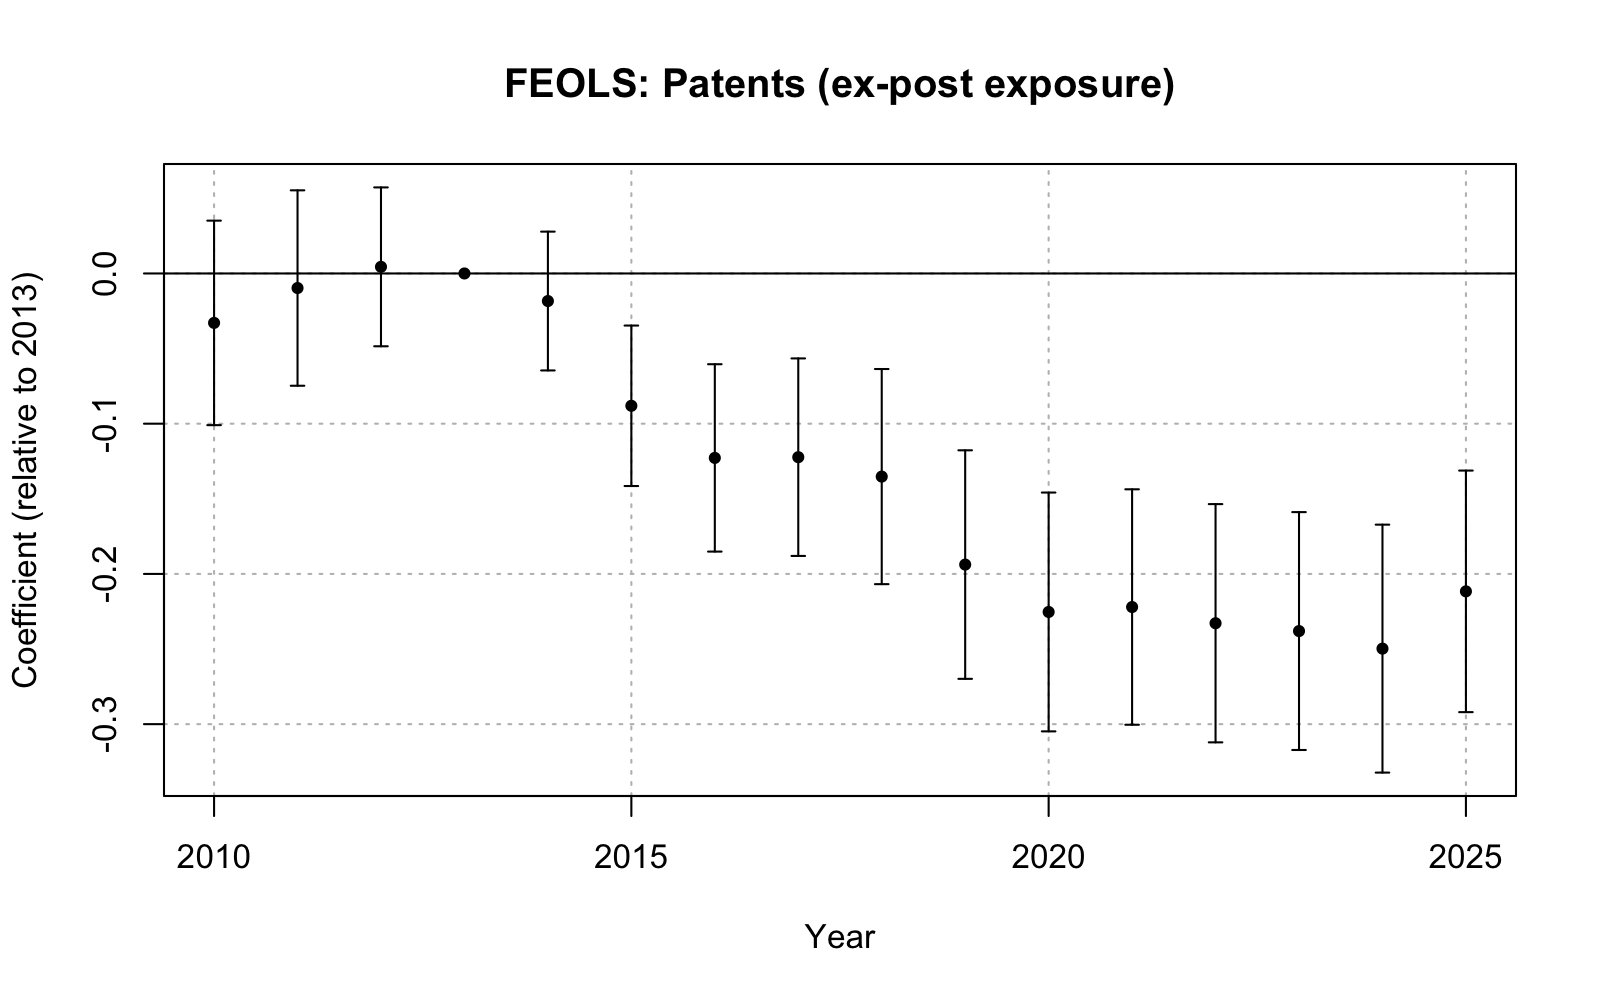
\includegraphics[width=\linewidth]{../output/RQ1/patent_feols_expost.png}
  \caption{FEOLS event study: patents, ex-post Medicaid exposure}
  \label{fig:rob_rq1_patent_feols_expost}
\end{figure}

\begin{figure}[!h]
  \centering
  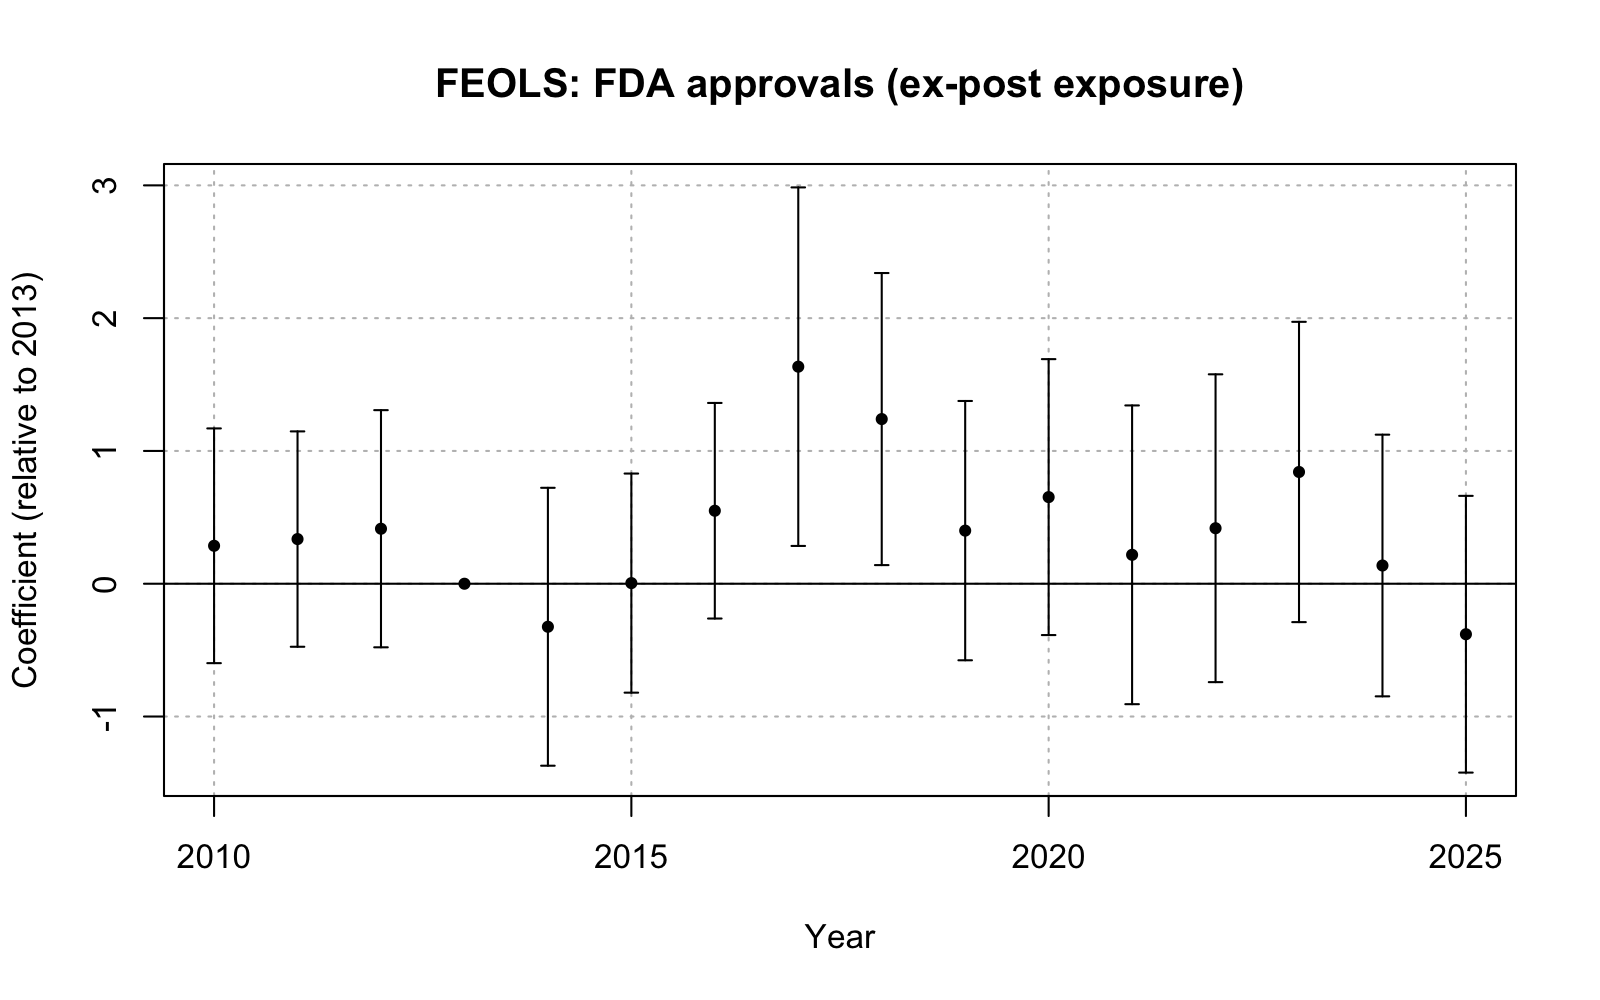
\includegraphics[width=\linewidth]{../output/RQ1/fda_feols_expost.png}
  \caption{FEOLS event study: FDA approvals, ex-post Medicaid exposure}
  \label{fig:rob_rq1_fda_feols_expost}
\end{figure}

\clearpage

\subsubsection{FE Poisson Estimation}

The baseline FEOLS specification models patent counts and FDA approvals linearly, although both outcomes are non-negative integer variables with substantial counts of zero. Consequently, the specification is re-estimated using a fixed-effects Poisson model, which therefore models the conditional mean of each of the innovation outcomes non-linearly. This allows for a robustness check on whether the baseline findings are sensitive to the linear treatment of the count outcomes, since the Poisson estimator remains consistent even when the outcome is overdispersed provided the conditional mean is correctly specified \citep{wooldridge1999distribution}.

The FE Poisson estimates for patents are consistent with the FEOLS results. Under the ex-ante specification, the pre-expansion coefficients are small and insignificant, providing support for the parallel trends assumption. The post-expansion coefficients are negative and grow in magnitude over time, peaking at $-1.474$ by 2024 and fall slightly in 2025, consistent with the FEOLS findings. Therefore, at its peak in 2024, a ten percentage point increase in Medicaid exposure corresponds to an approximate 14.7 percent decrease in patents on average. The ex-post FE Poisson estimates follow a similar trajectory, with the 2024 peak being more negative at $-2.021$.

While the FDA approval estimates under the Poisson model are uniformly negative, they still remain insignificant across both the ex-ante and ex-post specifications. This is a slight deviation from the baseline OLS results, where the FDA estimates fluctuate in sign, but both specifications agree that the innovation response at the approval stage remains statistically significant. The findings for both innovation outcomes are consistent between the linear and Poisson specifications, suggesting that the post-expansion patterns are not sensitive to modelling the count outcomes linearly.

\begin{figure}[!h]
  \centering
  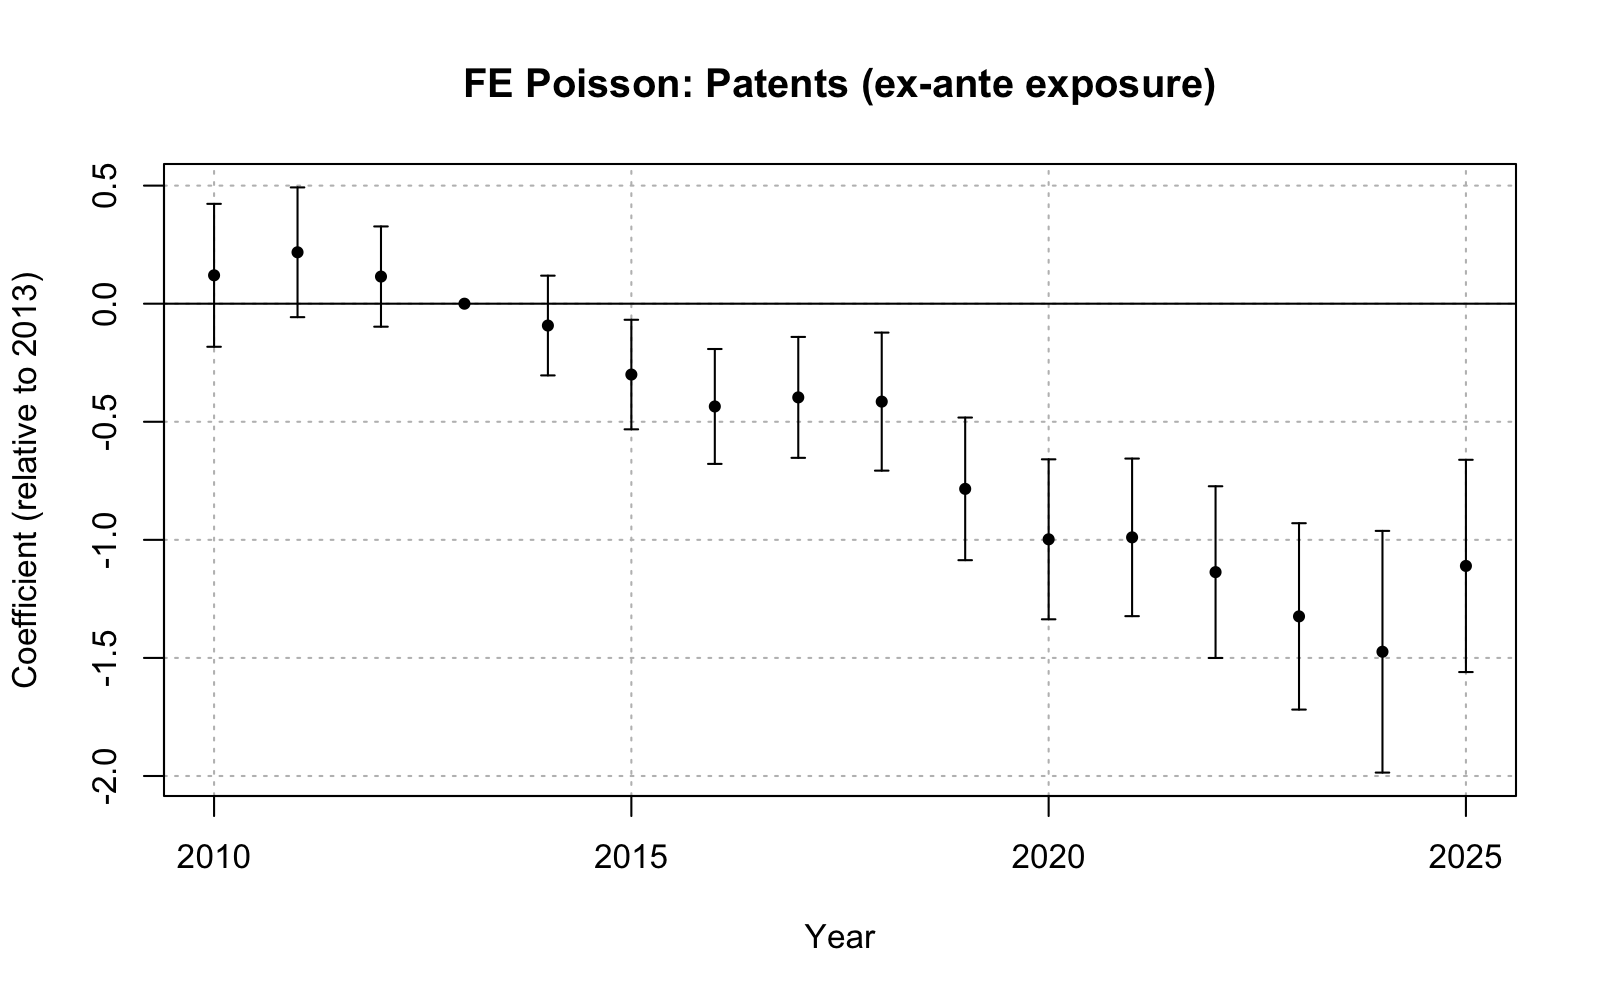
\includegraphics[width=\linewidth]{../output/RQ1/patent_poi_exante.png}
  \caption{FE Poisson event study: patents, ex-ante Medicaid exposure}
  \label{fig:rob_rq1_patent_poi_exante}
\end{figure}

\begin{figure}[!h]
  \centering
  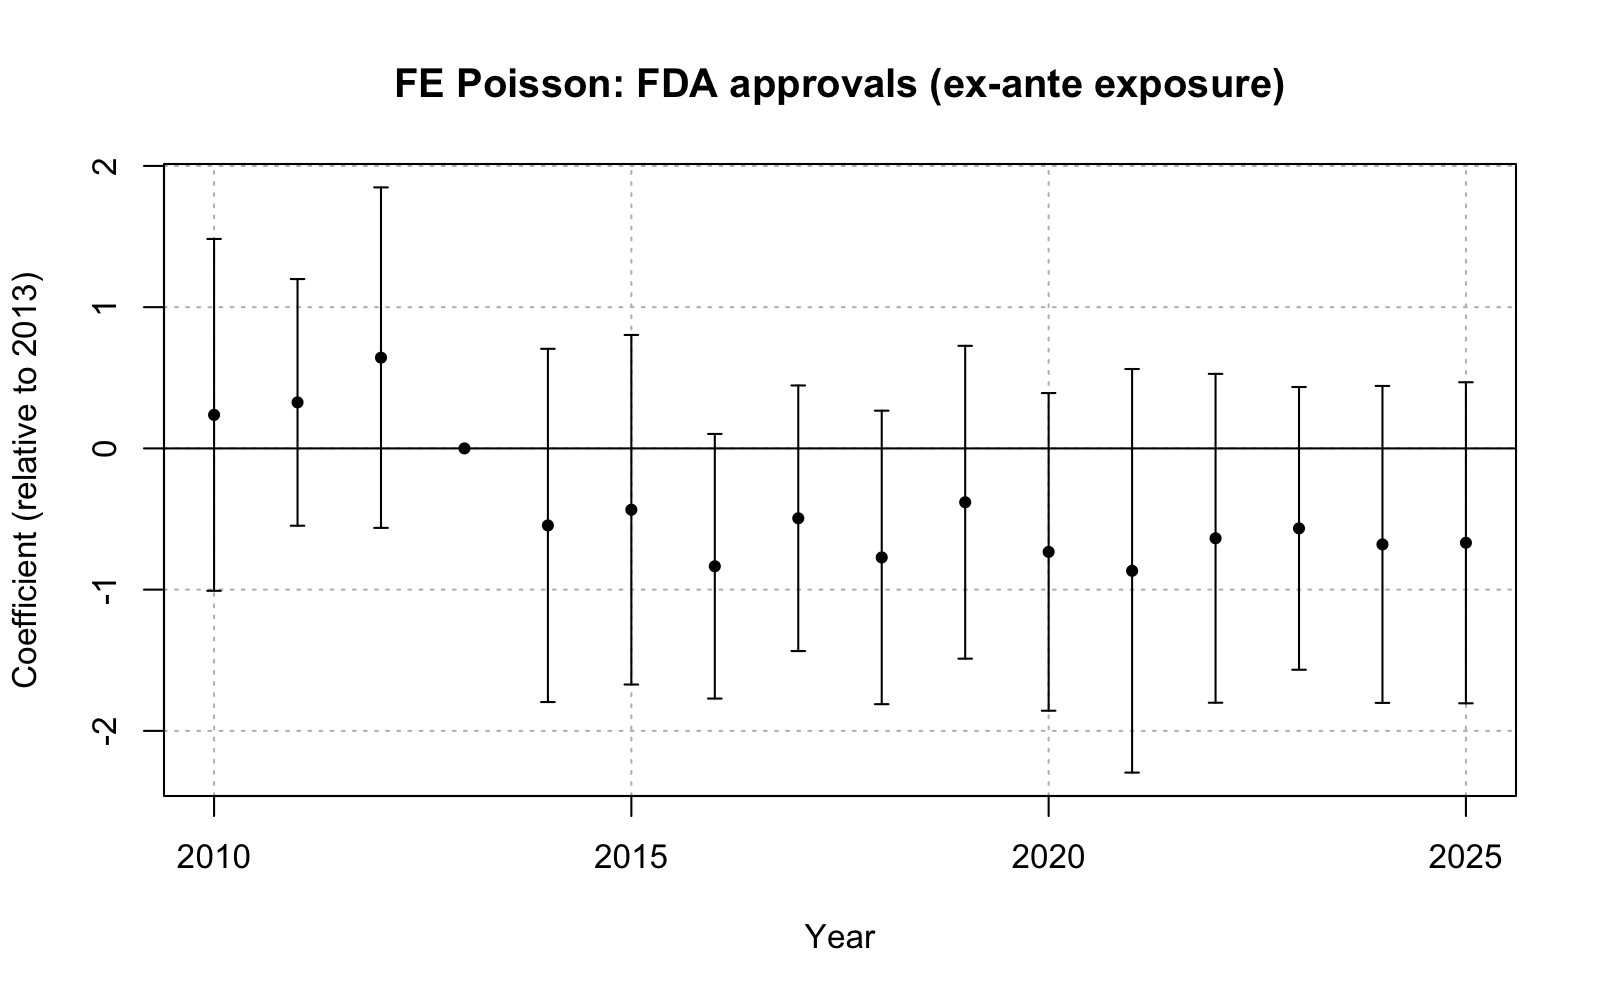
\includegraphics[width=\linewidth]{../output/RQ1/fda_poi_exante.png}
  \caption{FE Poisson event study: FDA approvals, ex-ante Medicaid exposure}
  \label{fig:rob_rq1_fda_poi_exante}
\end{figure}

\clearpage

\subsubsection{Binned Treatment Intensity}

The baseline specification treats exposure to the ACA as a continuous variable. As an alternative test, therapeutic classes are grouped into low, medium and high exposure bins, allowing for separate event-study coefficients to be estimated across different parts of the Medicaid exposure distribution. This relaxes the assumption of linearity in treatment effects imposed by the continuous specification, and examines whether the post-expansion response is concentrated among classes which are greater exposed to the Medicaid reform.

Therapeutic classes are grouped into the three bins based on their ex-ante Medicaid market shares, as reported in Table~\ref{tab:atc_bins}. Nervous system and cardiovascular drugs form the high-exposure bin, as their Medicaid market shares are substantially larger than other class shares. An approximate threshold of 10\% is used to distinguish between the medium and low bin classes, thus anti-infectives and dermatologicals form the medium-exposure bin.


\begingroup
\makeatletter
\renewenvironment{table}[1][tbp]{\@float{table}[#1]}{\end@float}
\makeatother
\begin{table}[htbp]
\centering
\caption{Pre-expansion Medicaid market shares and bin assignments}
\label{tab:atc_bins}
\begin{tabular}{llrl}
\toprule
\multicolumn{1}{c}{ATC} & \multicolumn{1}{c}{Therapeutic Area} & \multicolumn{1}{c}{Medicaid Share} & \multicolumn{1}{c}{Bin} \\
\midrule
N & Nervous system                  & 0.363 & High   \\
C & Cardiovascular system           & 0.215 & High   \\
J & Anti-infectives for systemic use & 0.120 & Medium \\
D & Dermatologicals                 & 0.099 & Medium \\
R & Respiratory system              & 0.085 & Low    \\
A & Alimentary tract and metabolism & 0.068 & Low    \\
M & Musculo-skeletal system         & 0.015 & Low    \\
H & Systemic hormonal preparations  & 0.012 & Low    \\
L & Antineoplastic and immunomodulating agents & 0.006 & Low \\
G & Genito-urinary system and sex hormones     & 0.006 & Low \\
S & Sensory organs                  & 0.005 & Low    \\
B & Blood and blood-forming organs  & 0.005 & Low    \\
V & Various                         & 0.000 & Low    \\
P & Antiparasitic products          & 0.000 & Low    \\
\bottomrule
\end{tabular}
\end{table}

\endgroup

The low exposure bin is omitted from the regression, so the coefficients for the high and medium bins are estimated relative to the low-exposure bin. The pre-expansion coefficients for both the high and medium-exposure patent bins are small and statistically insignificant, supporting the parallel trends assumption within each group. While the medium-exposure bin largely contain positive insignificant coefficients throughout the post-expansion period with a peak decline of $-0.02$ in 2025, the high-exposure bin exhibit a growing negative trajectory with coefficients reaching $-0.155$ by the same year. This reinforces the finding from RQ3 that the post-expansion patenting decline driven by classes at the upper end of the Medicaid exposure distribution. Importantly, the relative magnitude of the high and medium exposure coefficients is disproportionately larger than their respective Medicaid market shares. On average, exposure of the high bin is approximately $2.5$ times larger than the medium bin, yet the peak patent responses approximately differ by a factor of eight. This suggests that the relationship between Medicaid exposure and patenting may be convex, with the response intensifying at greater levels of exposure as opposed to scaling proportionally.

FDA approval estimates are statistically insignificant for both the high and medium-exposure bins throughout the sample period, and the pre-expansion coefficients are close to zero in both bins, supporting the parallel trends assumption. The absence of significant post-expansion effects for FDA approvals is consistent with the baseline findings and reinforces the interpretation that the innovation response has not yet propagated to the downstream approval stage. Unlike the patent results, the estimates from the FDA binned specification provide no evidence of a non-linear treatment effects across the Medicaid market share distribution, but this is driven by the absence of a detectable effect within each of the exposure bins rather than providing support for a linear relationship.

\clearpage

\begin{figure}[!h]
  \centering
  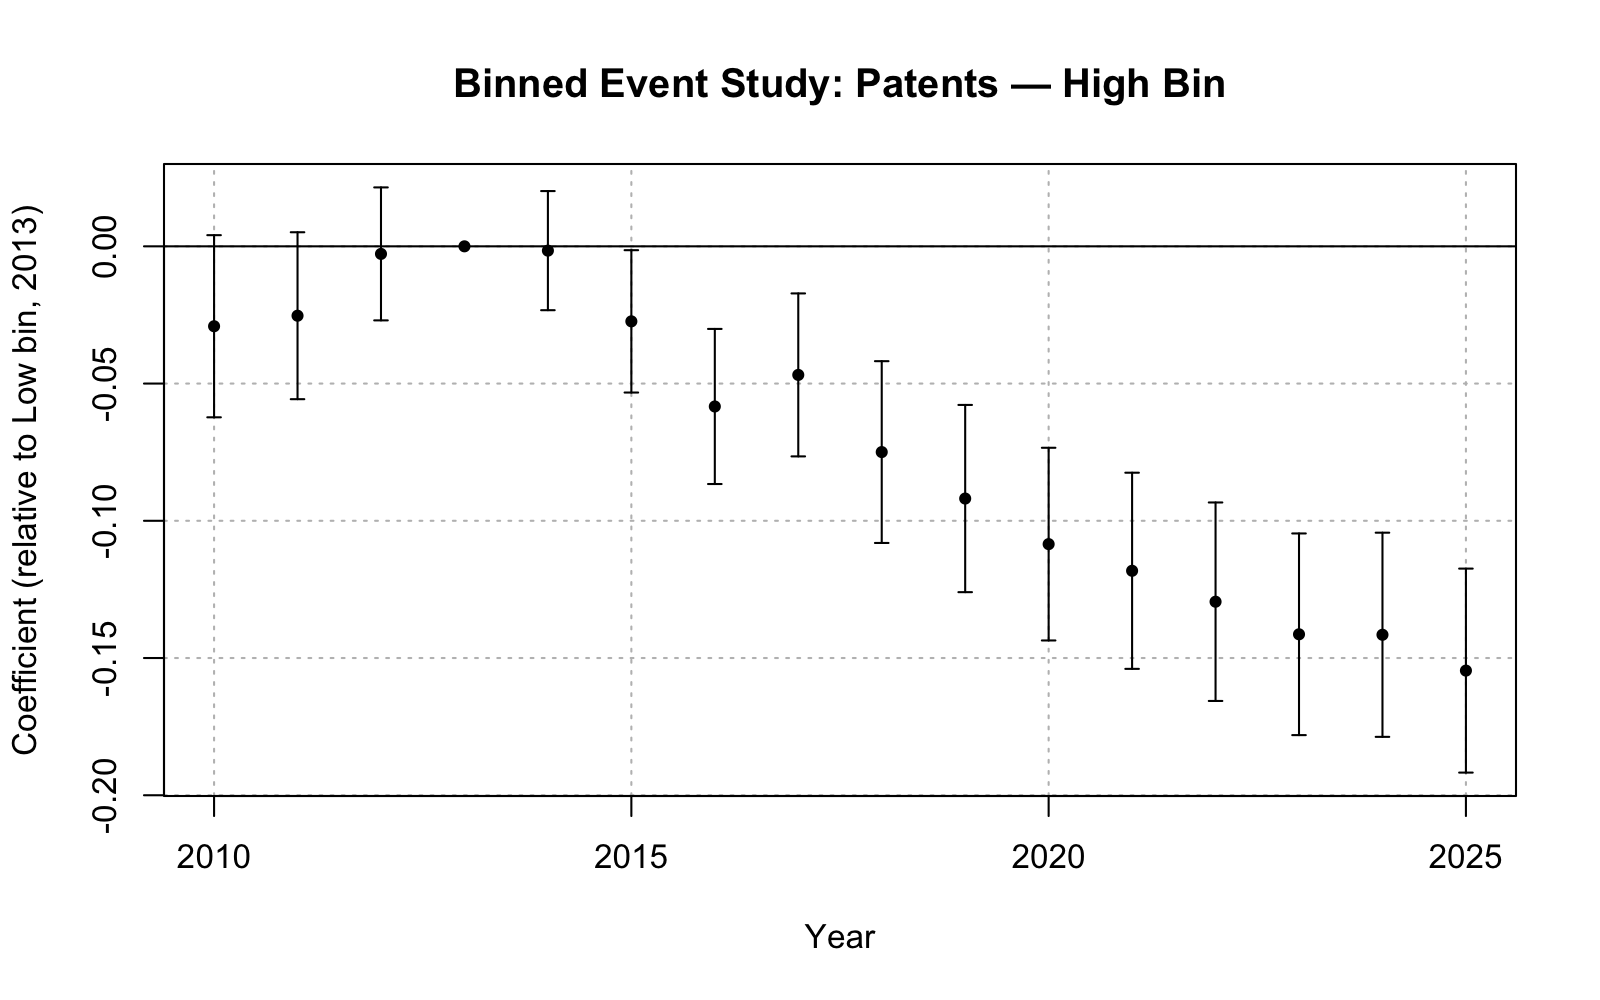
\includegraphics[width=\linewidth]{../output/robustness/binned_treatment/binned_patent_high_es.png}
  \caption{Binned event study: patents, high-exposure bin (N, C)}
  \label{fig:rob_binned_patent_high}
\end{figure}

\begin{figure}[!h]
  \centering
  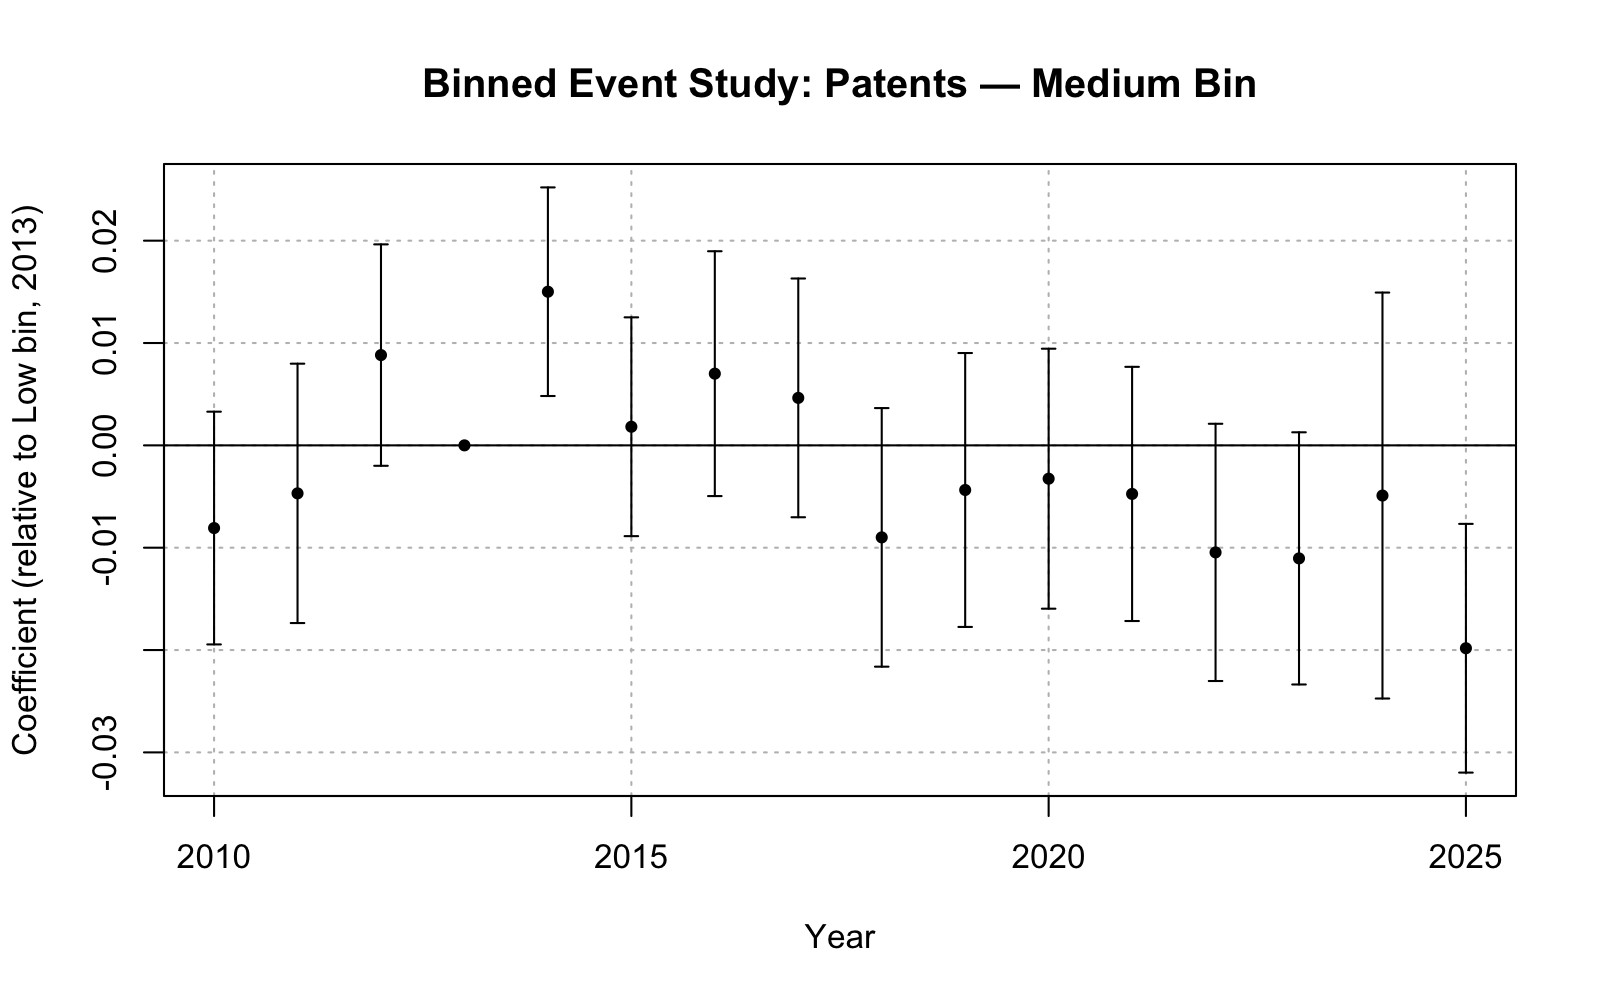
\includegraphics[width=\linewidth]{../output/robustness/binned_treatment/binned_patent_medium_es.png}
  \caption{Binned event study: patents, medium-exposure bin (J, D)}
  \label{fig:rob_binned_patent_medium}
\end{figure}

\clearpage

\begin{figure}[!h]
  \centering
  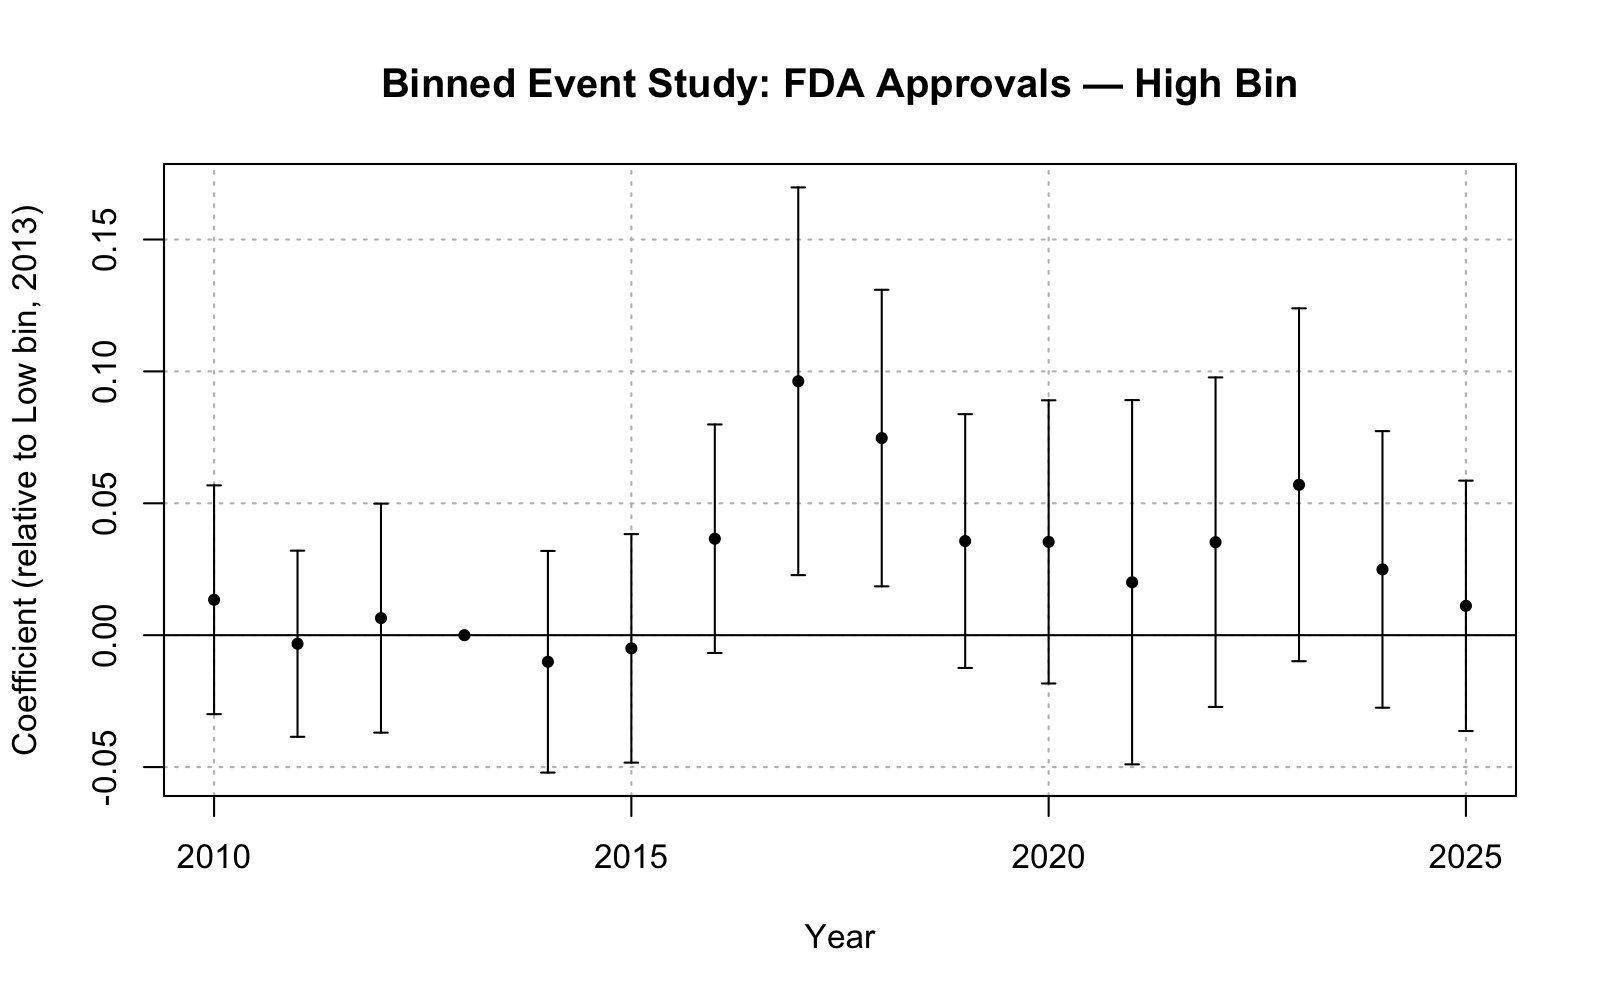
\includegraphics[width=\linewidth]{../output/robustness/binned_treatment/binned_fda_high_es.png}
  \caption{Binned event study: FDA approvals, high-exposure bin (N, C)}
  \label{fig:rob_binned_fda_high}
\end{figure}

\begin{figure}[!h]
  \centering
  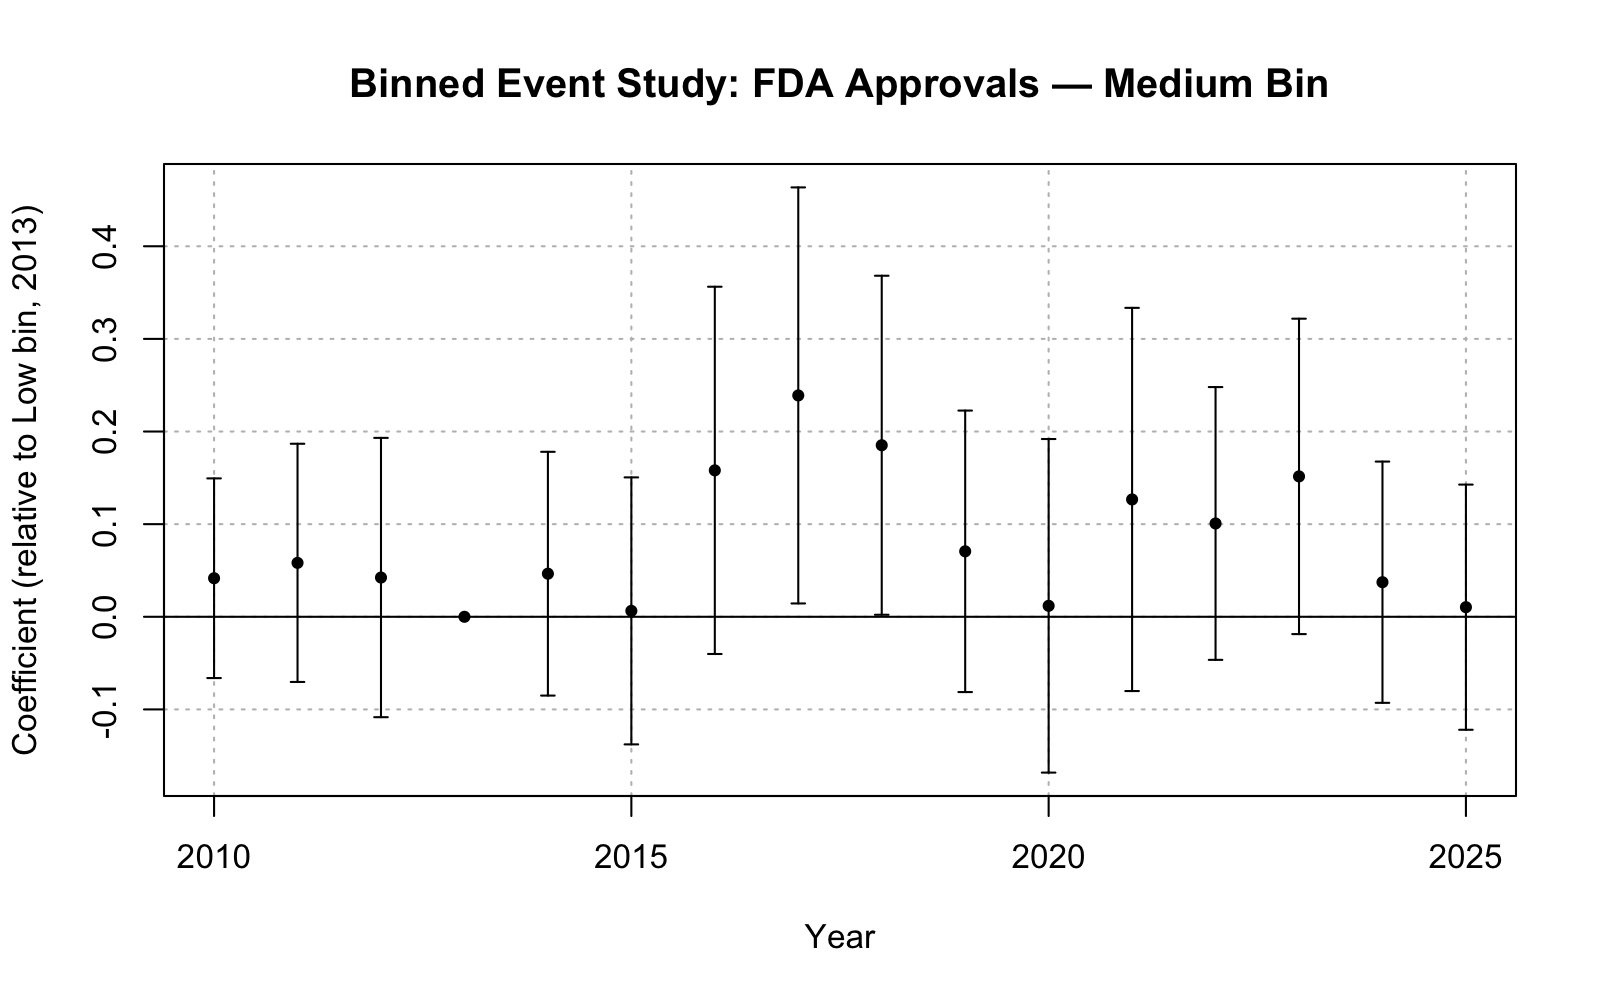
\includegraphics[width=\linewidth]{../output/robustness/binned_treatment/binned_fda_medium_es.png}
  \caption{Binned event study: FDA approvals, medium-exposure bin (J, D)}
  \label{fig:rob_binned_fda_medium}
\end{figure}

\clearpage

\subsubsection{Continuous Difference-in-Differences}

The binned event-study specification allowed for treatment effects to vary across the discrete groups, but the results were contingent on the boundaries specified for each exposure bin. Given this, the continuous difference-in-differences (Continuous DiD) estimator proposed by \citet{NBERw32117} is applied using the \texttt{contdid} R package \citep{contdid2025}. This estimator non-parametrically identifies dose-specific treatment effects at each exposure-level under the parallel trends assumption, thereby avoiding the need to discretise the treatment variable. Conventional TWFE estimators with continuous treatment can be difficult to interpret when treatment effects differ across the distribution of exposure level. The Continuous DiD estimator avoids this by aggregating the dose-specific estimates into event-study coefficients and assesses for pre-trends and post-treatment dynamics. The full set of coefficient estimates is reported in Table~\ref{tab:contdid_es}.

The Continuous DiD estimates for patents are consistent with the baseline results. The pre-expansion coefficients are small and statistically insignificant, supporting the parallel trends assumption. Notably, the coefficients are persistently significant from 2019 onwards, which is four years later than the 2015 onset under the baseline FEOLS model. This implies that the innovation response was not immediate as suggested by the baseline results, instead firms required several years to fully adjust their R\&D decisions in response to the expansion.

The FDA approval estimates under the Continuous DiD model are statistically insignificant throughout the entire period. The pre-period estimates are small and fluctuate around zero, while the post-expansion estimates are mostly positive. The absence of a clear FDA approval response to the Medicaid reform is therefore robust to modelling Medicaid exposure non-parametrically within the Continuous DiD framework.

Taken together, the results from the sensitivity analysis show that the main findings are robust to discretising market shares into exposure bins and using a non-parametric continuous DiD approach. Crucially, the sustained negative patent response remains visible under an estimator developed specifically for continuous-treatment DiD designs, while drug approvals do not appear to have a clear response to the ACA. The Continuous DiD estimates are also consistent with the binned analysis for highly exposed patents, while bins with medium exposure do not display a statistically significant response. This pattern is consistent with the class-level heterogeneity identified in RQ3, where nervous system and cardiovascular drugs were among the classes experiencing the greatest patent reductions.

\clearpage

\begin{figure}[!h]
  \centering
  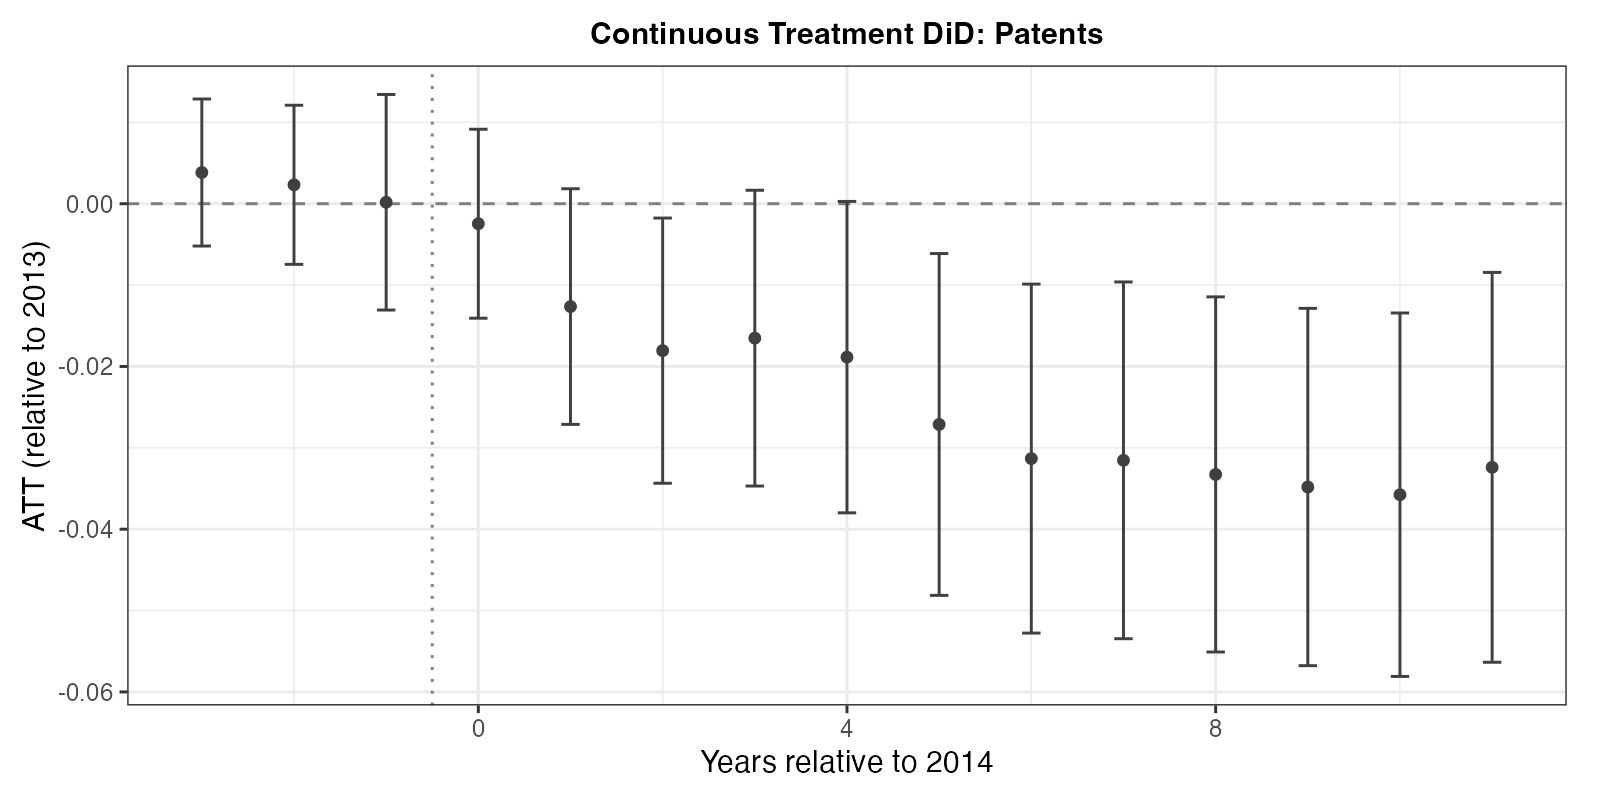
\includegraphics[width=\linewidth]{../output/robustness/contdid/contdid_patent_es.png}
  \caption{Continuous DiD event study: patents}
  \label{fig:rob_contdid_patent}
\end{figure}

\begin{figure}[!h]
  \centering
  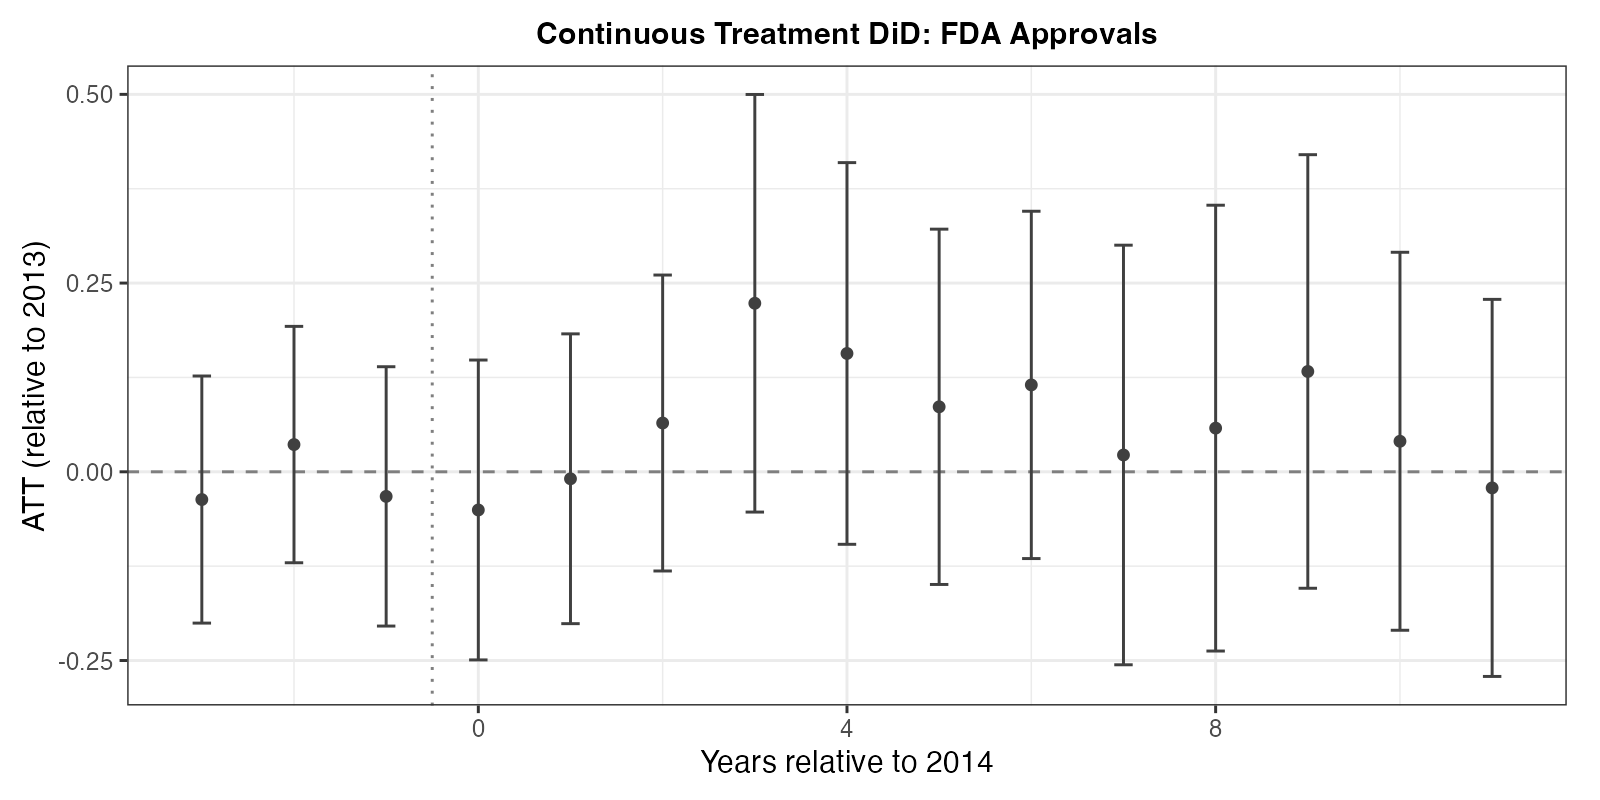
\includegraphics[width=\linewidth]{../output/robustness/contdid/contdid_fda_es.png}
  \caption{Continuous DiD event study: FDA approvals}
  \label{fig:rob_contdid_fda}
\end{figure}

\clearpage

% -----------------------------------------------------------------------
\subsection{RQ2: Medicaid Demand and PDL Exposure}
% -----------------------------------------------------------------------

\subsubsection{Ex-Post Medicaid Exposure}

The second specification jointly estimates the innovation response to Medicaid demand exposure and exposure to the PDL. Like RQ1, an ex-post market share measure is used to determine whether the estimates are sensitive to the construction of the exposure variable.

Once again, the ex-post Medicaid exposure coefficients for patents are nearly identical to the baseline results. The same reductions in Medicaid market share coefficients is observed, with the PDL exposure coefficient path also coinciding with the ex-ante model which saw negative coefficients from 2016 with significance from 2019. The pre-expansion coefficients for both the Medicaid and PDL measures remain small and statistically insignificant, supporting the parallel trends assumption even under the ex-post exposure construction.

The FDA approval coefficients are largely under the ex-post specification are statistically insignificant for both the Medicaid and PDL exposure measures, with isolated incidences of significance in a small number of post-expansion years. This aligns with the baseline finding that the innovation response has not yet reached the final stage of the R\&D pipeline. The agreement between the ex-ante and ex-post results therefore indicates that the decomposition into Medicaid demand and PDL exposure is not sensitive to the construction of exposure to Medicaid.

The FE Poisson, binned treatment, and continuous difference-in-differences estimators are not applied to the RQ2 specification. The joint estimation of two exposure variables under these alternative specifications is computationally demanding, and could not be completed with the device used for this study. Given this constraint, the alternative estimators are only used for the RQ1 specification where they are most informative for the aggregate response to the policy.

\clearpage

\begin{figure}[!h]
  \centering
  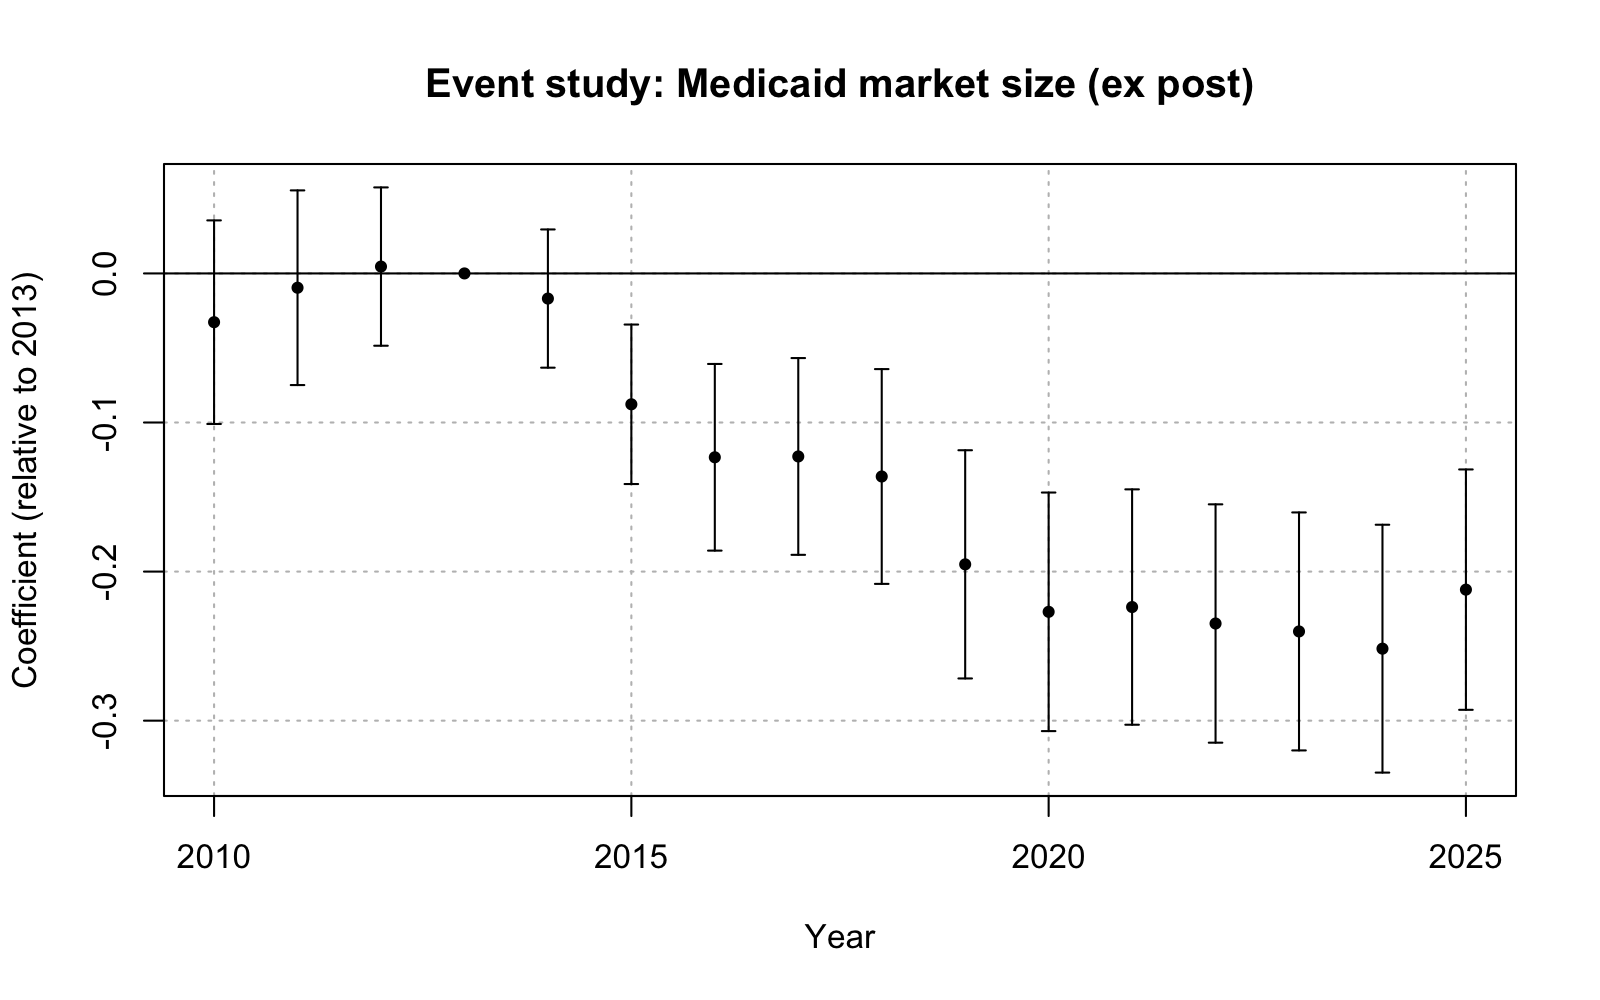
\includegraphics[width=\linewidth]{../output/RQ2/patent_feols_expost_medicaid.png}
  \caption{FEOLS event study: patents, Medicaid exposure (ex-post)}
  \label{fig:rob_rq2_patent_expost_medicaid}
\end{figure}

\begin{figure}[!h]
  \centering
  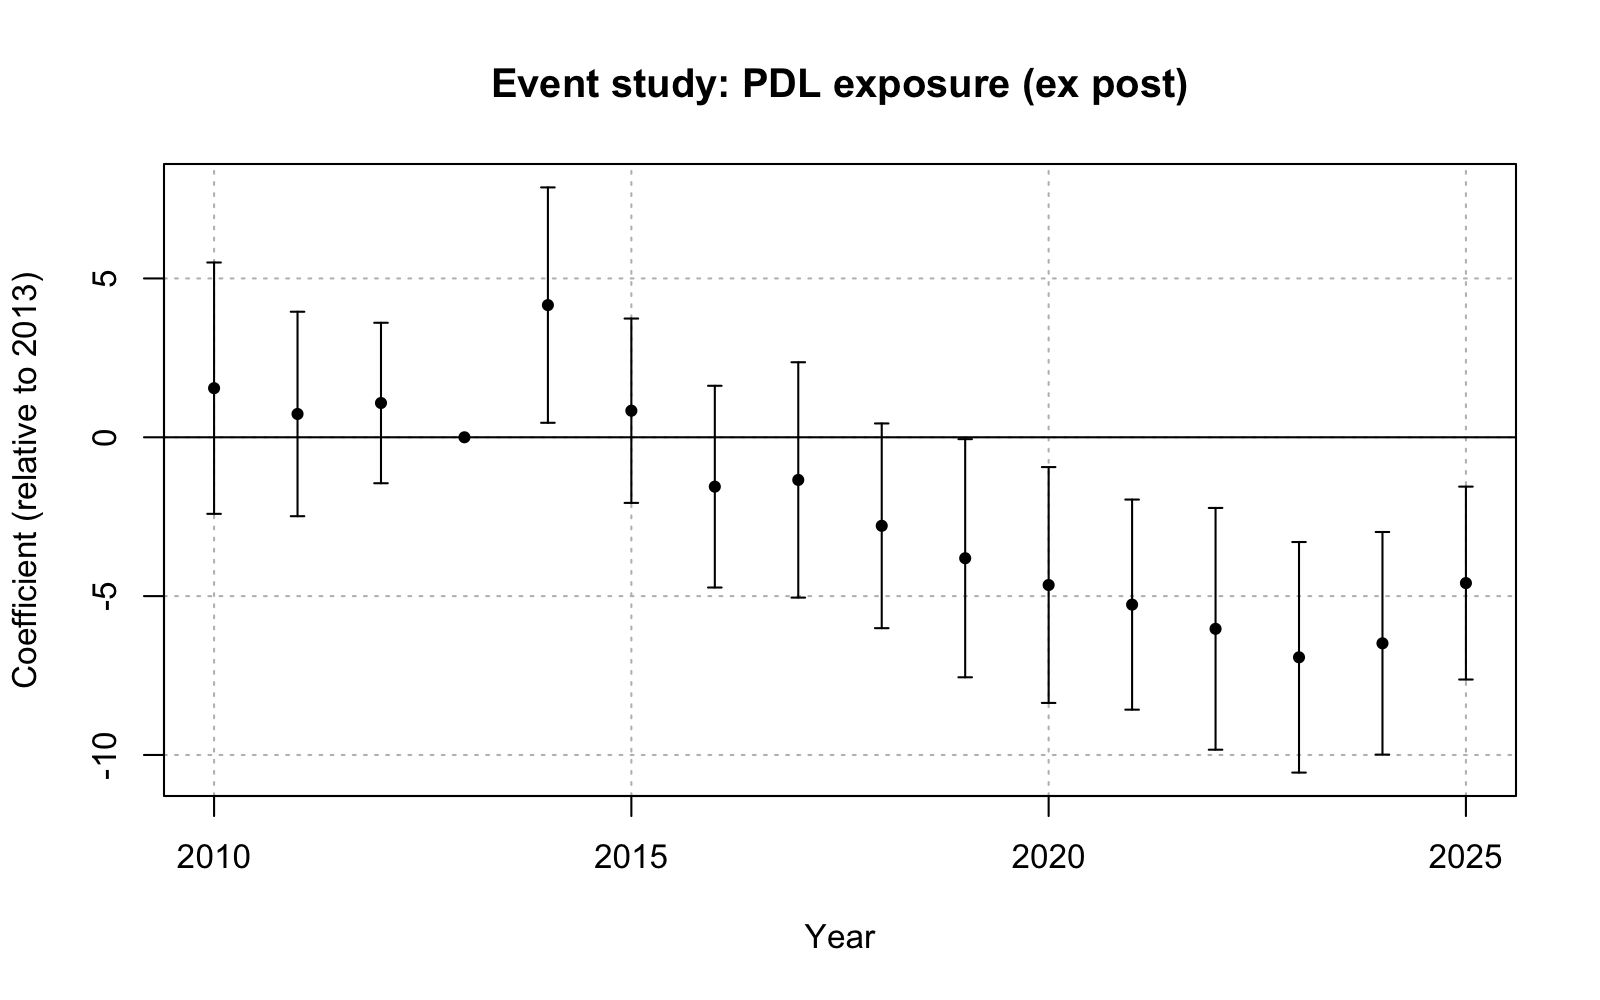
\includegraphics[width=\linewidth]{../output/RQ2/patent_feols_expost_pdl.png}
  \caption{FEOLS event study: patents, PDL exposure (ex-post)}
  \label{fig:rob_rq2_patent_expost_pdl}
\end{figure}

\clearpage

\begin{figure}[!h]
  \centering
  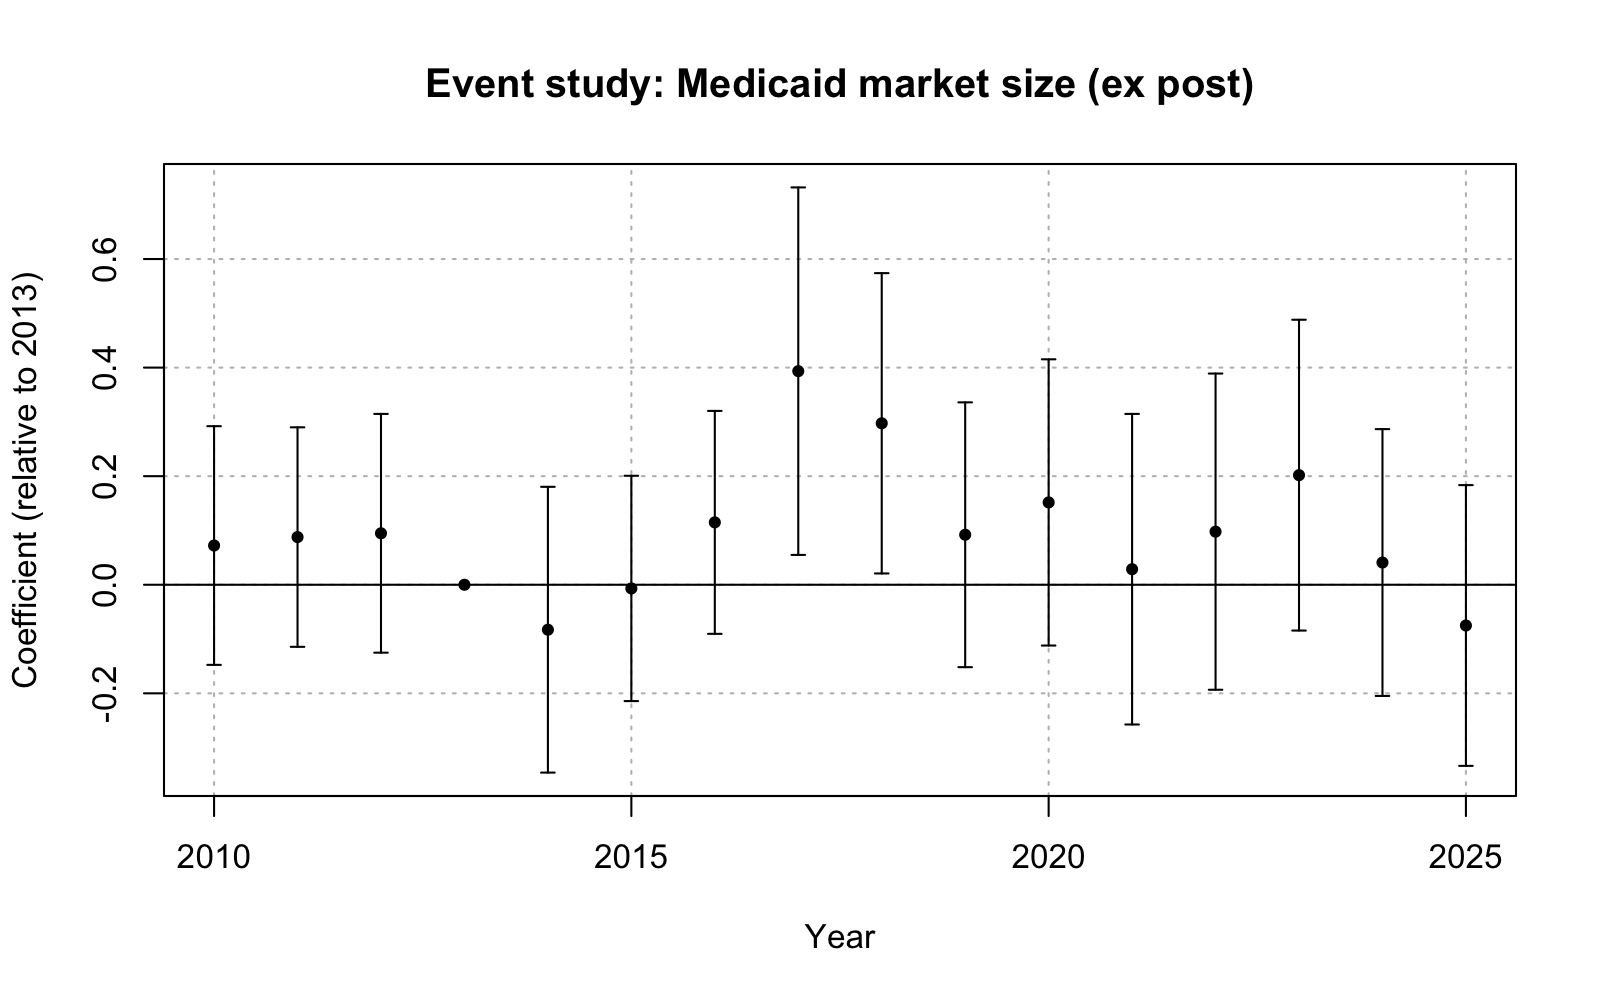
\includegraphics[width=\linewidth]{../output/RQ2/fda_feols_expost_medicaid.png}
  \caption{FEOLS event study: FDA approvals, Medicaid exposure (ex-post)}
  \label{fig:rob_rq2_fda_expost_medicaid}
\end{figure}

\begin{figure}[!h]
  \centering
  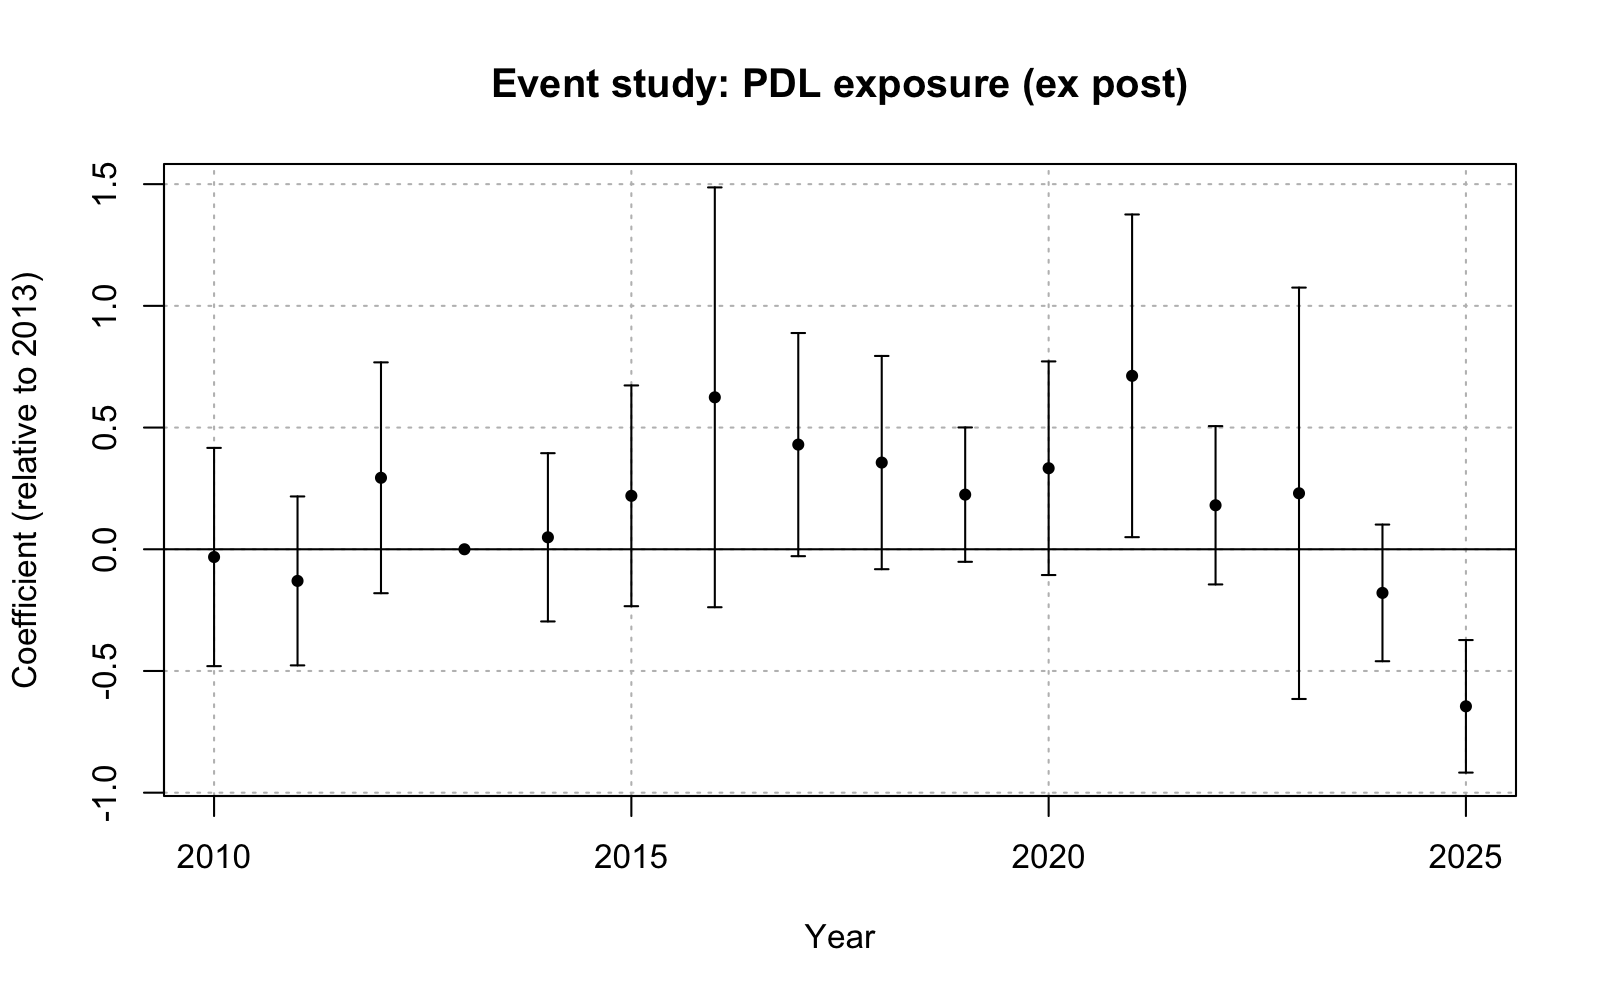
\includegraphics[width=\linewidth]{../output/RQ2/fda_feols_expost_pdl.png}
  \caption{FEOLS event study: FDA approvals, PDL exposure (ex-post)}
  \label{fig:rob_rq2_fda_expost_pdl}
\end{figure}

\clearpage

% -----------------------------------------------------------------------
\subsection{RQ3: Therapeutic-Class Heterogeneity}
% -----------------------------------------------------------------------

\subsubsection{Ex-Post Medicaid Exposure}

The RQ3 specification allows for heterogeneity in innovation behaviour to vary at ATC Level 1 therapeutic class. The ex-post exposure measure of Medicaid exposure is used as a robustness check.

\begin{center}
\begingroup\footnotesize
\begin{table}
\centering
\begin{talltblr}[         %% tabularray outer open
entry=none,label=none,
note{}={* p \num{< 0.05}, ** p \num{< 0.01}, *** p \num{< 0.001}},
]                     %% tabularray outer close
{                     %% tabularray inner open
colspec={Q[]Q[]Q[]},
column{2,3}={}{halign=c,},
column{1}={}{halign=l,},
hline{26}={1,2,3}{solid, black, 0.05em},
}                     %% tabularray inner close
\toprule
& Patents & FDA Approvals \\ \midrule
Medicaid Share × ATC = A & \num{-0.157}*** & \num{1.301}**  \\
& (\num{0.031})   & (\num{0.420})  \\
Medicaid Share × ATC = B & \num{0.151}***  & \num{-0.121}   \\
& (\num{0.027})   & (\num{0.784})  \\
Medicaid Share × ATC = C & \num{-0.094}*** & \num{0.373}    \\
& (\num{0.015})   & (\num{0.278})  \\
Medicaid Share × ATC = D & \num{-0.017}    & \num{0.881}**  \\
& (\num{0.062})   & (\num{0.337})  \\
Medicaid Share × ATC = G & \num{0.032}     & \num{-1.058}   \\
& (\num{0.049})   & (\num{1.121})  \\
Medicaid Share × ATC = H & \num{0.619}***  & \num{0.446}    \\
& (\num{0.096})   & (\num{0.530})  \\
Medicaid Share × ATC = J & \num{0.035}     & \num{-0.078}   \\
& (\num{0.034})   & (\num{0.089})  \\
Medicaid Share × ATC = L & \num{0.443}     & \num{-0.244}   \\
& (\num{0.578})   & (\num{2.115})  \\
Medicaid Share × ATC = M & \num{-0.212}*** & \num{0.017}    \\
& (\num{0.048})   & (\num{0.858})  \\
Medicaid Share × ATC = N & \num{-0.174}*** & \num{0.047}    \\
& (\num{0.039})   & (\num{0.101})  \\
Medicaid Share × ATC = R & \num{0.005}     & \num{0.178}    \\
& (\num{0.003})   & (\num{0.130})  \\
Medicaid Share × ATC = S & \num{0.105}***  & \num{6.473}*   \\
& (\num{0.020})   & (\num{3.004})  \\
Num. obs.                & \num{19617728}  & \num{561600}   \\
R2                       & \num{0.247}     & \num{0.235}    \\
\bottomrule
\end{talltblr}
\end{table}

\endgroup
\end{center}


The ex-post estimates are broadly consistent with the ex-ante baseline. Therapeutic classes that exhibited significant negative patent responses under ex-ante exposure, continue to display significant negative coefficients under the ex-post measure. Additionally, positive patent responses are still observed for therapeutic classes relating to blood related drugs, hormonal preparations, and sensory organs. Simiarly, the FDA approval coefficients are aligned with their ex-ante results - significant positive responses for alimentary tract and dermatologicals, and no class are recorded to have a significant reduction in approvals. The results aligning between the two exposure measures indicates that the baseline class-level heterogeneity in innovation response is not driven by the choice of exposure measure.

\subsubsection{Parallel Trends}

The RQ3 triple-difference specification does not take the form of an event study, as the estimation of class-specific dynamic coefficients would be computationally intensive. Consequently, pre-trends coefficients cannot be estimated directly, so the parallel trends assumption cannot be tested for in the same manner as RQ1 and RQ2. Since ATC class V is the omitted from the regressions, it is the reference group for the DDD models. In this context, this specifically indicates that absent the ACA, the relationship between Medicaid exposure and changes in innovation outcomes would have evolved similarly across therapeutic classes relative to class V. The results from earlier the earlier analyses and the model structure can provide evidence to support the plausibility of this assumption.

First, the RQ1 and RQ2 event studies consistently display small and statistically insignificant pre-expansion coefficients across all specifications, including FEOLS, FE Poisson, binned treatment and the continuous DiD approach. Therefore, therapeutic classes with differing levels of Medicaid exposure followed similar innovation trajectories prior to the ACA expansion. Since the same Medicaid exposure measure and firm-class panels are used for RQ3, the evidence for parallel trends from RQ1 and RQ2 provide support for the key identifying assumption of RQ3.

Third, as discussed in the methodology, a violation of parallel trends would require an additional shock around 2014 that differentially affected innovation within therapeutic classes such that it was correlated with exposure to Medicaid. There are no clear candidates for such a confounding shock.

\clearpage

\bibliographystyle{apalike}
\bibliography{references}

\clearpage
\appendix

% -----------------------------------------------------------------------
\section{Robustness Regression Tables}
% -----------------------------------------------------------------------

\subsection{RQ1: Ex-Post FEOLS}

\begingroup\footnotesize
\begin{table}
\centering
\begin{talltblr}[         %% tabularray outer open
entry=none,label=none,
note{}={* p \num{< 0.05}, ** p \num{< 0.01}, *** p \num{< 0.001}},
]                     %% tabularray outer close
{                     %% tabularray inner open
width=\linewidth,
colspec={Q[]X[]X[]},
column{2,3}={}{halign=c,},
column{1}={}{halign=l,},
hline{32}={1,2,3}{solid, black, 0.05em},
}                     %% tabularray inner close
\toprule
& Patents & FDA Approvals \\ \midrule
2010 × Medicaid Share & \num{-0.033}    & \num{0.286}   \\
                      & (\num{0.035})   & (\num{0.450}) \\
2011 × Medicaid Share & \num{-0.010}    & \num{0.336}   \\
                      & (\num{0.033})   & (\num{0.413}) \\
2012 × Medicaid Share & \num{0.004}     & \num{0.414}   \\
                      & (\num{0.027})   & (\num{0.455}) \\
2014 × Medicaid Share & \num{-0.018}    & \num{-0.324}  \\
                      & (\num{0.024})   & (\num{0.533}) \\
2015 × Medicaid Share & \num{-0.088}**  & \num{0.005}   \\
                      & (\num{0.027})   & (\num{0.420}) \\
2016 × Medicaid Share & \num{-0.123}*** & \num{0.550}   \\
                      & (\num{0.032})   & (\num{0.413}) \\
2017 × Medicaid Share & \num{-0.122}*** & \num{1.635}*  \\
                      & (\num{0.034})   & (\num{0.688}) \\
2018 × Medicaid Share & \num{-0.135}*** & \num{1.240}*  \\
                      & (\num{0.037})   & (\num{0.560}) \\
2019 × Medicaid Share & \num{-0.194}*** & \num{0.400}   \\
                      & (\num{0.039})   & (\num{0.497}) \\
2020 × Medicaid Share & \num{-0.225}*** & \num{0.652}   \\
                      & (\num{0.041})   & (\num{0.529}) \\
2021 × Medicaid Share & \num{-0.222}*** & \num{0.218}   \\
                      & (\num{0.040})   & (\num{0.573}) \\
2022 × Medicaid Share & \num{-0.233}*** & \num{0.418}   \\
                      & (\num{0.040})   & (\num{0.590}) \\
2023 × Medicaid Share & \num{-0.238}*** & \num{0.842}   \\
                      & (\num{0.040})   & (\num{0.576}) \\
2024 × Medicaid Share & \num{-0.250}*** & \num{0.137}   \\
                      & (\num{0.042})   & (\num{0.502}) \\
2025 × Medicaid Share & \num{-0.212}*** & \num{-0.380}  \\
                      & (\num{0.041})   & (\num{0.531}) \\
Num. obs.             & \num{5281696}   & \num{151200}  \\
R2                    & \num{0.534}     & \num{0.609}   \\
\bottomrule
\end{talltblr}
\end{table}

\endgroup

\clearpage

\subsection{RQ1: FE Poisson (Ex-Ante)}

\begingroup\footnotesize
\begin{table}
\centering
\begin{talltblr}[         %% tabularray outer open
entry=none,label=none,
note{}={* p \num{< 0.05}, ** p \num{< 0.01}, *** p \num{< 0.001}},
]                     %% tabularray outer close
{                     %% tabularray inner open
width=\linewidth,
colspec={Q[]X[]X[]},
column{2,3}={}{halign=c,},
column{1}={}{halign=l,},
hline{32}={1,2,3}{solid, black, 0.05em},
}                     %% tabularray inner close
\toprule
& Patents & FDA Approvals \\ \midrule
2010 × Medicaid Share & \num{0.120}     & \num{0.237}   \\
                      & (\num{0.154})   & (\num{0.636}) \\
2011 × Medicaid Share & \num{0.218}     & \num{0.326}   \\
                      & (\num{0.140})   & (\num{0.446}) \\
2012 × Medicaid Share & \num{0.115}     & \num{0.643}   \\
                      & (\num{0.108})   & (\num{0.615}) \\
2014 × Medicaid Share & \num{-0.092}    & \num{-0.545}  \\
                      & (\num{0.108})   & (\num{0.638}) \\
2015 × Medicaid Share & \num{-0.300}*   & \num{-0.434}  \\
                      & (\num{0.118})   & (\num{0.632}) \\
2016 × Medicaid Share & \num{-0.435}*** & \num{-0.834}  \\
                      & (\num{0.124})   & (\num{0.478}) \\
2017 × Medicaid Share & \num{-0.397}**  & \num{-0.495}  \\
                      & (\num{0.131})   & (\num{0.480}) \\
2018 × Medicaid Share & \num{-0.415}**  & \num{-0.772}  \\
                      & (\num{0.149})   & (\num{0.530}) \\
2019 × Medicaid Share & \num{-0.784}*** & \num{-0.381}  \\
                      & (\num{0.154})   & (\num{0.565}) \\
2020 × Medicaid Share & \num{-0.998}*** & \num{-0.733}  \\
                      & (\num{0.173})   & (\num{0.574}) \\
2021 × Medicaid Share & \num{-0.989}*** & \num{-0.867}  \\
                      & (\num{0.170})   & (\num{0.729}) \\
2022 × Medicaid Share & \num{-1.137}*** & \num{-0.637}  \\
                      & (\num{0.186})   & (\num{0.594}) \\
2023 × Medicaid Share & \num{-1.324}*** & \num{-0.566}  \\
                      & (\num{0.201})   & (\num{0.511}) \\
2024 × Medicaid Share & \num{-1.474}*** & \num{-0.680}  \\
                      & (\num{0.261})   & (\num{0.573}) \\
2025 × Medicaid Share & \num{-1.110}*** & \num{-0.668}  \\
                      & (\num{0.229})   & (\num{0.580}) \\
Num. obs.             & \num{1300944}   & \num{42176}   \\
\bottomrule
\end{talltblr}
\end{table}

\endgroup

\clearpage

\subsection{RQ1: FE Poisson (Ex-Post)}

\begingroup\footnotesize
\begin{table}
\centering
\begin{talltblr}[         %% tabularray outer open
entry=none,label=none,
note{}={* p \num{< 0.05}, ** p \num{< 0.01}, *** p \num{< 0.001}},
]                     %% tabularray outer close
{                     %% tabularray inner open
width=\linewidth,
colspec={Q[]X[]X[]},
column{2,3}={}{halign=c,},
column{1}={}{halign=l,},
hline{32}={1,2,3}{solid, black, 0.05em},
}                     %% tabularray inner close
\toprule
& Patents & FDA Approvals \\ \midrule
2010 × Medicaid Share & \num{0.129}     & \num{0.453}   \\
                      & (\num{0.157})   & (\num{0.869}) \\
2011 × Medicaid Share & \num{0.240}     & \num{1.138}   \\
                      & (\num{0.145})   & (\num{0.687}) \\
2012 × Medicaid Share & \num{0.124}     & \num{1.250}   \\
                      & (\num{0.115})   & (\num{0.863}) \\
2014 × Medicaid Share & \num{-0.086}    & \num{-0.711}  \\
                      & (\num{0.106})   & (\num{0.996}) \\
2015 × Medicaid Share & \num{-0.367}**  & \num{-0.431}  \\
                      & (\num{0.119})   & (\num{0.725}) \\
2016 × Medicaid Share & \num{-0.515}*** & \num{-0.788}  \\
                      & (\num{0.129})   & (\num{0.660}) \\
2017 × Medicaid Share & \num{-0.533}*** & \num{-0.278}  \\
                      & (\num{0.134})   & (\num{0.735}) \\
2018 × Medicaid Share & \num{-0.556}*** & \num{-0.595}  \\
                      & (\num{0.157})   & (\num{0.713}) \\
2019 × Medicaid Share & \num{-0.998}*** & \num{-0.625}  \\
                      & (\num{0.167})   & (\num{0.764}) \\
2020 × Medicaid Share & \num{-1.293}*** & \num{-0.916}  \\
                      & (\num{0.190})   & (\num{0.839}) \\
2021 × Medicaid Share & \num{-1.313}*** & \num{-0.909}  \\
                      & (\num{0.188})   & (\num{0.910}) \\
2022 × Medicaid Share & \num{-1.564}*** & \num{-0.657}  \\
                      & (\num{0.203})   & (\num{0.775}) \\
2023 × Medicaid Share & \num{-1.803}*** & \num{-0.618}  \\
                      & (\num{0.224})   & (\num{0.695}) \\
2024 × Medicaid Share & \num{-2.021}*** & \num{-0.969}  \\
                      & (\num{0.266})   & (\num{0.854}) \\
2025 × Medicaid Share & \num{-1.692}*** & \num{-1.254}  \\
                      & (\num{0.262})   & (\num{0.892}) \\
Num. obs.             & \num{1300944}   & \num{42176}   \\
\bottomrule
\end{talltblr}
\end{table}

\endgroup

\begin{figure}[!h]
  \centering
  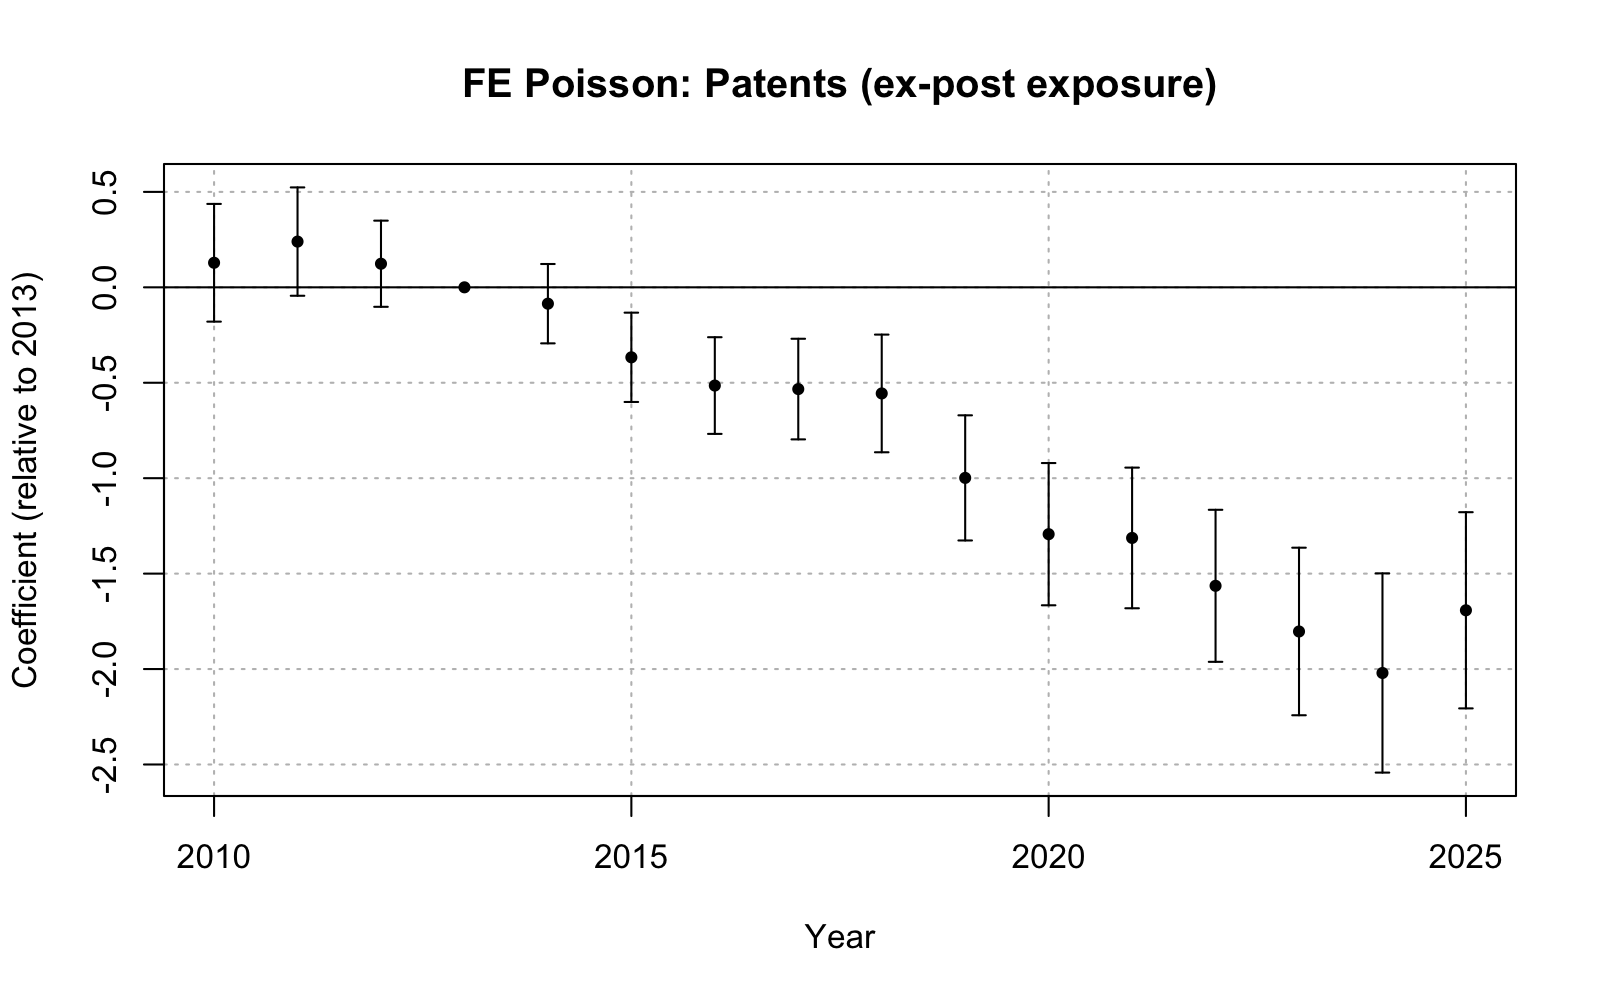
\includegraphics[width=\linewidth]{../output/RQ1/patent_poi_expost.png}
  \caption{FE Poisson event study: patents, ex-post Medicaid exposure}
  \label{fig:rob_rq1_patent_poi_expost}
\end{figure}

\begin{figure}[!h]
  \centering
  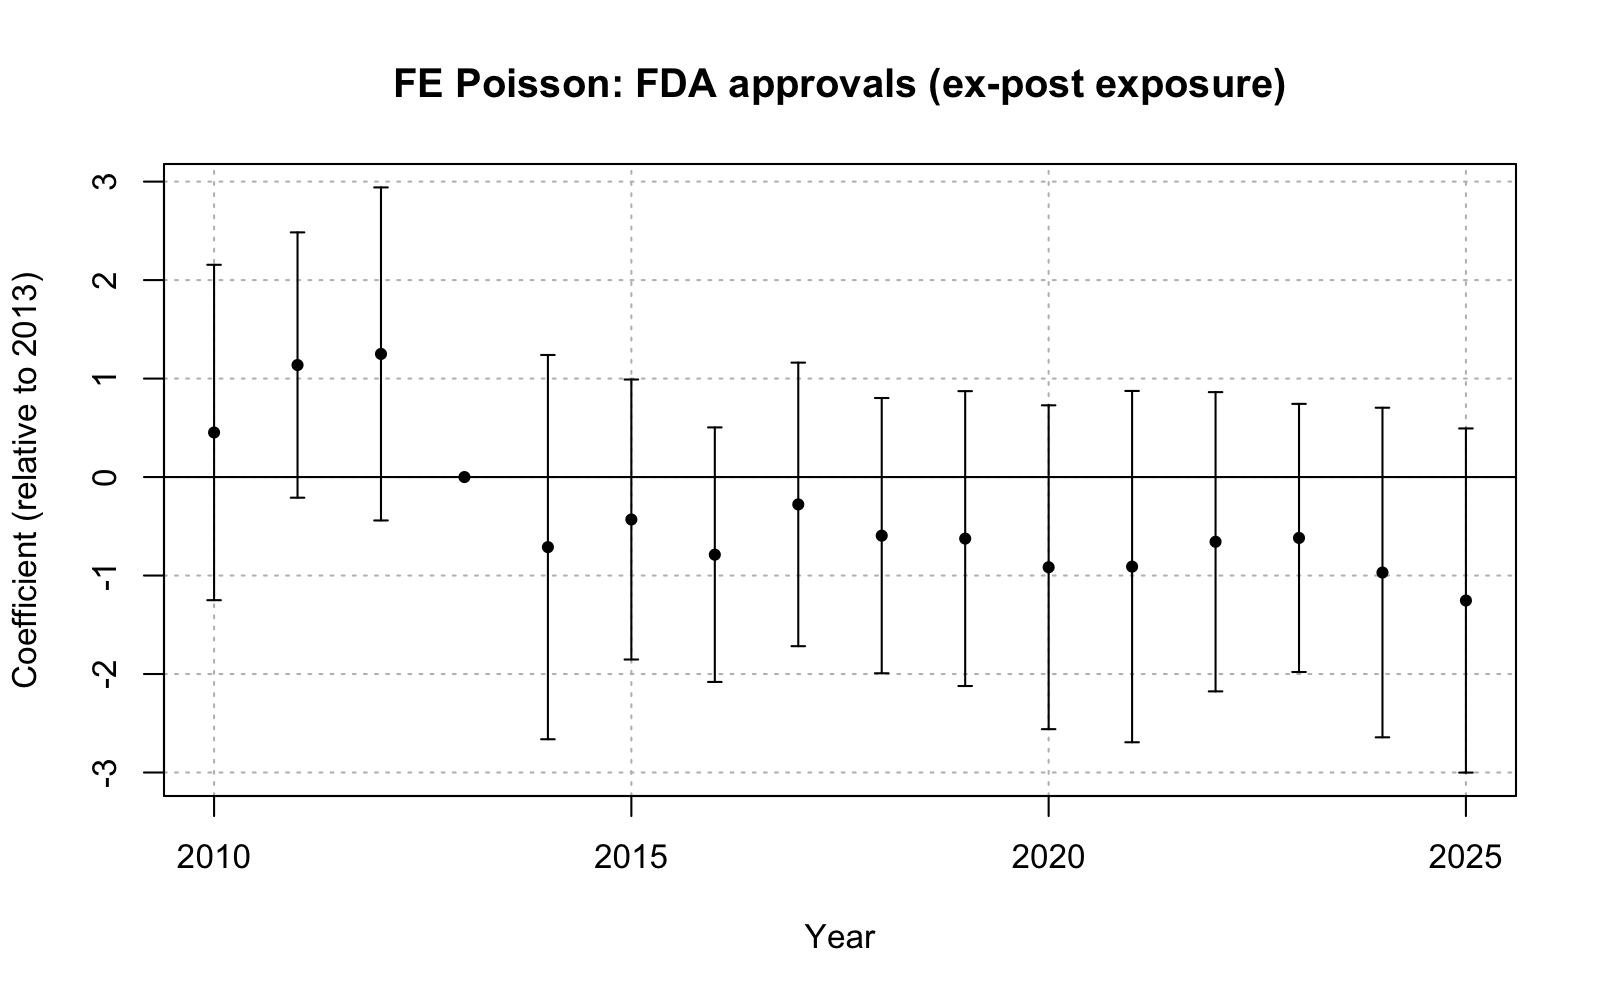
\includegraphics[width=\linewidth]{../output/RQ1/fda_poi_expost.png}
  \caption{FE Poisson event study: FDA approvals, ex-post Medicaid exposure}
  \label{fig:rob_rq1_fda_poi_expost}
\end{figure}

\clearpage

\subsection{RQ1: Binned Treatment}

\begingroup\footnotesize
\begin{table}
\centering
\begin{talltblr}[         %% tabularray outer open
entry=none,label=none,
note{}={* p \num{< 0.05}, ** p \num{< 0.01}, *** p \num{< 0.001}},
]                     %% tabularray outer close
{                     %% tabularray inner open
width=\linewidth,
colspec={Q[]X[]X[]X[]X[]},
column{2,3,4,5}={}{halign=c,},
column{1}={}{halign=l,},
hline{33}={1,2,3,4,5}{solid, black, 0.05em},
}                     %% tabularray inner close
\toprule
& \SetCell[c=2]{c} Patents && \SetCell[c=2]{c} FDA Approvals & \\
& Medium Bin & High Bin & Medium Bin & High Bin \\ \midrule
2010 & \num{-0.008}    & \num{-0.029}    & \num{0.042}   & \num{0.085}   \\
     & (\num{0.006})   & (\num{0.017})   & (\num{0.055}) & (\num{0.140}) \\
2011 & \num{-0.005}    & \num{-0.025}    & \num{0.058}   & \num{-0.064}  \\
     & (\num{0.006})   & (\num{0.016})   & (\num{0.065}) & (\num{0.105}) \\
2012 & \num{0.009}     & \num{-0.003}    & \num{0.042}   & \num{0.033}   \\
     & (\num{0.006})   & (\num{0.012})   & (\num{0.077}) & (\num{0.121}) \\
2014 & \num{0.015}**   & \num{-0.002}    & \num{0.047}   & \num{-0.091}  \\
     & (\num{0.005})   & (\num{0.011})   & (\num{0.067}) & (\num{0.130}) \\
2015 & \num{0.002}     & \num{-0.027}*   & \num{0.006}   & \num{-0.005}  \\
     & (\num{0.005})   & (\num{0.013})   & (\num{0.073}) & (\num{0.148}) \\
2016 & \num{0.007}     & \num{-0.058}*** & \num{0.158}   & \num{0.070}   \\
     & (\num{0.006})   & (\num{0.014})   & (\num{0.101}) & (\num{0.130}) \\
2017 & \num{0.005}     & \num{-0.047}**  & \num{0.239}*  & \num{0.326}   \\
     & (\num{0.006})   & (\num{0.015})   & (\num{0.114}) & (\num{0.181}) \\
2018 & \num{-0.009}    & \num{-0.075}*** & \num{0.185}*  & \num{0.213}   \\
     & (\num{0.006})   & (\num{0.017})   & (\num{0.093}) & (\num{0.155}) \\
2019 & \num{-0.004}    & \num{-0.092}*** & \num{0.071}   & \num{0.206}   \\
     & (\num{0.007})   & (\num{0.017})   & (\num{0.077}) & (\num{0.162}) \\
2020 & \num{-0.003}    & \num{-0.108}*** & \num{0.012}   & \num{0.141}   \\
     & (\num{0.006})   & (\num{0.018})   & (\num{0.092}) & (\num{0.142}) \\
2021 & \num{-0.005}    & \num{-0.118}*** & \num{0.127}   & \num{-0.048}  \\
     & (\num{0.006})   & (\num{0.018})   & (\num{0.105}) & (\num{0.182}) \\
2022 & \num{-0.010}    & \num{-0.129}*** & \num{0.101}   & \num{0.040}   \\
     & (\num{0.006})   & (\num{0.018})   & (\num{0.075}) & (\num{0.184}) \\
2023 & \num{-0.011}    & \num{-0.141}*** & \num{0.152}   & \num{0.154}   \\
     & (\num{0.006})   & (\num{0.019})   & (\num{0.087}) & (\num{0.182}) \\
2024 & \num{-0.005}    & \num{-0.142}*** & \num{0.037}   & \num{0.070}   \\
     & (\num{0.010})   & (\num{0.019})   & (\num{0.066}) & (\num{0.146}) \\
2025 & \num{-0.020}**  & \num{-0.155}*** & \num{0.010}   & \num{0.032}   \\
     & (\num{0.006})   & (\num{0.019})   & (\num{0.067}) & (\num{0.153}) \\
Num. obs. & \SetCell[c=2]{c} \num{5281696} && \SetCell[c=2]{c} \num{151200} & \\
R2        & \SetCell[c=2]{c} \num{0.534}   && \SetCell[c=2]{c} \num{0.609}  & \\
\bottomrule
\end{talltblr}
\end{table}

\endgroup

\clearpage

\subsection{RQ1: Continuous Difference-in-Differences}

\begingroup
\makeatletter
\renewenvironment{table}[1][tbp]{\@float{table}[#1]}{\end@float}
\makeatother
\footnotesize
\begin{table}
\centering
\begin{talltblr}[         %% tabularray outer open
entry=none,label=none,
note{}={* 95\% uniform confidence band does not cover 0},
]                     %% tabularray outer close
{                     %% tabularray inner open
colspec={Q[]Q[]Q[]},
column{2,3}={}{halign=c,},
column{1}={}{halign=l,},
hline{8}={1,2,3}{solid, black, 0.05em},
}                     %% tabularray inner close
\toprule
Event Time & Patents & FDA Approvals \\ \midrule %% TinyTableHeader
-3 & \num{0.0038} & \num{-0.0368} \\
   & (\num{0.0034}) & (\num{0.0602}) \\
-2 & \num{0.0023} & \num{0.0361} \\
   & (\num{0.0037}) & (\num{0.0576}) \\
-1 & \num{0.0002} & \num{-0.0326} \\
   & (\num{0.0050}) & (\num{0.0632}) \\
0 & \num{-0.0025} & \num{-0.0506} \\
   & (\num{0.0044}) & (\num{0.0731}) \\
1 & \num{-0.0126} & \num{-0.0092} \\
   & (\num{0.0055}) & (\num{0.0706}) \\
2 & \num{-0.0181}* & \num{0.0646} \\
   & (\num{0.0062}) & (\num{0.0721}) \\
3 & \num{-0.0165} & \num{0.2233} \\
   & (\num{0.0069}) & (\num{0.1018}) \\
4 & \num{-0.0189} & \num{0.1568} \\
   & (\num{0.0073}) & (\num{0.0930}) \\
5 & \num{-0.0271}* & \num{0.0861} \\
   & (\num{0.0080}) & (\num{0.0866}) \\
6 & \num{-0.0313}* & \num{0.1151} \\
   & (\num{0.0082}) & (\num{0.0846}) \\
7 & \num{-0.0315}* & \num{0.0223} \\
   & (\num{0.0084}) & (\num{0.1022}) \\
8 & \num{-0.0333}* & \num{0.0579} \\
   & (\num{0.0083}) & (\num{0.1086}) \\
9 & \num{-0.0348}* & \num{0.1329} \\
   & (\num{0.0084}) & (\num{0.1056}) \\
10 & \num{-0.0358}* & \num{0.0404} \\
   & (\num{0.0085}) & (\num{0.0921}) \\
11 & \num{-0.0324}* & \num{-0.0213} \\
   & (\num{0.0091}) & (\num{0.0919}) \\
\bottomrule
\end{talltblr}
\end{table}

\endgroup

\clearpage

\subsection{RQ2: Ex-Post FEOLS}

\begingroup\footnotesize
\begin{table}
\centering
\begin{talltblr}[         %% tabularray outer open
entry=none,label=none,
note{}={* p \num{< 0.05}, ** p \num{< 0.01}, *** p \num{< 0.001}},
]                     %% tabularray outer close
{                     %% tabularray inner open
width=\linewidth,
colspec={Q[]X[]X[]X[]X[]},
column{2,3,4,5}={}{halign=c,},
column{1}={}{halign=l,},
hline{33}={1,2,3,4,5}{solid, black, 0.05em},
}                     %% tabularray inner close
\toprule
& \SetCell[c=2]{c} Patents && \SetCell[c=2]{c} FDA Approvals & \\
& Medicaid Market Share & PDL Exposure & Medicaid Market Share & PDL Exposure \\ \midrule
2010 & \num{-0.033}    & \num{1.546}     & \num{0.285}   & \num{0.046}   \\
     & (\num{0.035})   & (\num{2.018})   & (\num{0.448}) & (\num{0.807}) \\
2011 & \num{-0.010}    & \num{0.734}     & \num{0.344}   & \num{-0.257}  \\
     & (\num{0.033})   & (\num{1.642})   & (\num{0.412}) & (\num{0.711}) \\
2012 & \num{0.005}     & \num{1.079}     & \num{0.371}   & \num{1.395}   \\
     & (\num{0.027})   & (\num{1.289})   & (\num{0.447}) & (\num{0.912}) \\
2014 & \num{-0.017}    & \num{4.161}*    & \num{-0.338}  & \num{0.398}   \\
     & (\num{0.024})   & (\num{1.890})   & (\num{0.536}) & (\num{0.647}) \\
2015 & \num{-0.088}**  & \num{0.836}     & \num{-0.037}  & \num{1.158}   \\
     & (\num{0.027})   & (\num{1.480})   & (\num{0.422}) & (\num{0.881}) \\
2016 & \num{-0.123}*** & \num{-1.554}    & \num{0.456}   & \num{2.642}   \\
     & (\num{0.032})   & (\num{1.620})   & (\num{0.418}) & (\num{1.682}) \\
2017 & \num{-0.123}*** & \num{-1.342}    & \num{1.566}*  & \num{1.924}   \\
     & (\num{0.034})   & (\num{1.890})   & (\num{0.690}) & (\num{0.992}) \\
2018 & \num{-0.136}*** & \num{-2.787}    & \num{1.181}*  & \num{1.683}   \\
     & (\num{0.037})   & (\num{1.644})   & (\num{0.563}) & (\num{1.021}) \\
2019 & \num{-0.195}*** & \num{-3.807}*   & \num{0.359}   & \num{1.171}*  \\
     & (\num{0.039})   & (\num{1.912})   & (\num{0.498}) & (\num{0.591}) \\
2020 & \num{-0.227}*** & \num{-4.650}*   & \num{0.598}   & \num{1.585}   \\
     & (\num{0.041})   & (\num{1.894})   & (\num{0.537}) & (\num{0.942}) \\
2021 & \num{-0.224}*** & \num{-5.267}**  & \num{0.103}   & \num{3.110}*  \\
     & (\num{0.040})   & (\num{1.687})   & (\num{0.583}) & (\num{1.393}) \\
2022 & \num{-0.235}*** & \num{-6.029}**  & \num{0.381}   & \num{0.994}   \\
     & (\num{0.041})   & (\num{1.941})   & (\num{0.593}) & (\num{0.653}) \\
2023 & \num{-0.240}*** & \num{-6.926}*** & \num{0.798}   & \num{1.191}   \\
     & (\num{0.041})   & (\num{1.851})   & (\num{0.583}) & (\num{1.737}) \\
2024 & \num{-0.252}*** & \num{-6.485}*** & \num{0.154}   & \num{-0.447}  \\
     & (\num{0.042})   & (\num{1.788})   & (\num{0.501}) & (\num{0.589}) \\
2025 & \num{-0.212}*** & \num{-4.589}**  & \num{-0.347}  & \num{-1.113}  \\
     & (\num{0.041})   & (\num{1.549})   & (\num{0.525}) & (\num{0.908}) \\
Num. obs. & \SetCell[c=2]{c} \num{5281696} && \SetCell[c=2]{c} \num{151200} & \\
R2        & \SetCell[c=2]{c} \num{0.535}   && \SetCell[c=2]{c} \num{0.609}  & \\
\bottomrule
\end{talltblr}
\end{table}

\endgroup

\end{document}

\input{theoretical_model}
\documentclass[12pt]{article}
\usepackage{geometry}
\geometry{a4paper, portrait, margin=1in}

% --- Math Packages ---
\usepackage{amsmath}
\usepackage{amssymb}
\usepackage{amsfonts}
\usepackage{amsthm}

% --- Graphics & Diagrams ---
\usepackage{graphicx}
\usepackage{tikz}
\usetikzlibrary{shapes, arrows, positioning}

% --- Formatting ---
\usepackage{parskip}
\usepackage[hidelinks]{hyperref}
\usepackage{natbib}
\usepackage{enumitem}
\pagestyle{plain}

% --- Word count (requires compiling with --shell-escape) ---
\newcommand{\wordcount}{%
  \immediate\write18{texcount -sum -1 \jobname.tex 2>/dev/null | python3 -c "import sys; n=sys.stdin.read().strip(); print(f'{int(n):,}') if n.isdigit() else print('?')" > \jobname.wc}%
  \input{\jobname.wc}%
}

\title{MPhil Thesis: Conclusion}
\author{Mohammad-Shah Karim}
\date{May 2026}

\begin{document}

\ifdefined\isdraft\else
\maketitle
\begin{center}
  \small Word count: \wordcount
\end{center}
\fi

\section{Directions for Further Research}

The empirical and theoretical analysis presented in this thesis is subject to several limitations. This section discusses the most important of these and identifies directions in which future work could extend the analysis.

\subsection{Clinical Trial Outcomes}

This thesis chooses to study patenting and drug approvals to capture the innovation stages before and after clinical-trials studied by \citet{NBERw28755}. Clinical trials are an intermediate position between these two outcomes; incorporating clinical-trial data would complete the pipeline comparison, thereby allowing the analysis to trace the innovation response across all three stages. Given the scope of this study, this extension was not feasible within the scope of the present study. \citeauthor{NBERw28755} utilise a proprietary clinical trial data supplied by Cortellis. Constructing a comparable panel from ClinicalTrials.gov would require substantial work. The wording of study titles vary substantially and do not always identify the relevant disease area explicitly. Mapping these records to therapeutic-classes would therefore require imperfect text-based classification. Future work utilising Cortellis could assess whether the negative patenting response identified in this thesis is mirrored at the trial stage.

\subsection{PDL Measurement}

The PDL exposure measure used in this thesis is constructed from the Texas Vendor Drug Program, as this is the only state that has made the full formulary history available in a machine-readable format. While the representativeness analysis indicates that the Texas PDL shares substantial overlap with the New York and Washington, overlap with California is considerably weaker, reflecting differences in state-level formulary structures. This introduces measurement error into the PDL exposure variable, since firms classified as having heavy exposure to the PDL in Texas may be less exposed to it in other states. Consequently, the estimated innovations response to PDL exposure is likely to be attenuated towards zero, and should be interpreted as a plausible lower bound. Further work could construct a multi-state PDL exposure measure using additional formulary records, and average these across states to obtain a more representative measure ofa firm's overall exposure to Medicaid's PDL.

\subsection{Therapeutic Classification}

The analysis aggregates all outcomes to a coarse clinical outcome - ATC Level 1. This can contain drugs with substantially different clinical profiles and competitive environments, so within-class innovation heterogeneity may be masked. This is particularly relevant for the heterogeneity analysis in RQ3, where differences in innovation responses may remain hidden even where the ATC Level 1 estimates appear null or weak. Finer classification such as ATC Levels 2 or 3 may allow the analysis to distinguish between sub-therapeutic areas, but would come at the cost of an increase in panel dimensionality and therefore computational demands. Patents are classified using a CPC-to-ATC crosswalk, and extending to more granular ATC levels would require a mapping that may be noisy.

\subsection{Alternative Estimators for the Joint Specification}

The FE Poisson, binned-treatment, and continuous DiD estimators are applied to the RQ1 specification but not the RQ2 specification separating the innovation responses to both Medicaid and PDL exposure. Extending these estimators to the joint specification exceeded the computational power of the device used for this thesis, due to the size of the firm-class panels and the additional interactions required. The RQ2 estimates are instead supported by the ex-ante and ex-post exposure comparison with the use of FEOLS, but were not subject to equivalent estimator-level sensitivity analysis. Future work could therefore use greater computational capacity to assess whether the decomposition of demand and PDL exposure is robust alternative models.

\subsection{The Theoretical Model}

The theoretical model developed is an illustrative simplification designed to formalise how the Medicaid expansion can reduce innovation incentives through the procurement design. The model restricts competition to two firms competing for access within each therapeutic class, and assumes that the winner of the price stage receives the entire Medicaid market. In reality, several manufacturers compete for PDL authorisation within a therapeutic class, and multiple products may receive preferred placement. The model therefore abstracts from an oligopolistic structure to a duopoly setting in order to isolate the interaction between market size, rebate extraction, and the rent gap rather than the exact number of firms. An $N$-firm extension would allow for the examination of how rebate pressure scales with the number of clinically viable competitors, and whether the Medicaid expansion causes marginal firms to exit Medicaid-relevant therapeutic areas entirely rather than simply reducing innovation effort.

\section{Conclusion}

This thesis has examined whether the ACA Medicaid expansion raised pharmaceutical innovation, and whether the response depended on firms' exposure to Medicaid's procurement institutions. Conventionally, an expansion in expected demand should increase the expected return to R\&D \citep{finkelstein2004static, dubois2015market}. However, the Medicaid setting alters this prediction, as the additional demand is subject to statutory rebates, supplemental rebate negotiations, and drug-list bargaining. To study this question, the analysis constructed novel firm-therapeutic-class panels linking both patent records and FDA drug approvals to Medicaid prescription data, and PDL placement over 2010-2025.

The main empirical finding is that therapeutic classes with greater exposure to Medicaid experienced a persistent decline in patenting following the 2014 reform, while FDA approvals had an inconclusive response. The divergence between patents and FDA approvals is consistent with the changes in patenting behaviour appearing earlier in the R\&D pipeline, with insufficient time passing for changes in drug development to reach the approval stage. This interpretation explains the null effect documented in clinical trials by \citet{NBERw28755}.

A decomposition of innovation behaviour by demand and PDL exposure revealed that firms with greater exposure to Medicaid's PDL experienced additional declines in patenting beyond the demand channel. The PDL counterfactual analysis provides further suggestive support for this where firms securing The aggregate decline in patenting is not uniform across the pharmaceutical industry, with the declines being concentrated in classes with higher exposure to Medicaid and greater levels of drug substitutability. However, classes with lower drug substitutability instead saw innovation responses consistent with the standard market-size prediction, with a rise in patent applications. The PDL counterfactual adds further to this nuanced mechanism, where firms passing only one stage of the PDL selection process experience the largest declines in patenting, while firms securing full preferred placement exhibited declines, albeit smaller ones.

The theoretical model formalises this procurement-based interpretation. Since rebate extraction strengthened with the Medicaid market expansion, additional demand can lower expected returns to R\&D. This effect is likelier to hold for more clinically substitutable drugs, where Medicaid's bargaining position for deeper rebates is stronger. Notably, the model identifies the gap between monopoly and competitive profits as the key object linking pricing pressure to innovation incentives. Policies that shrink this gap therefore reduce equilibrium effort immediately and in the future period through an internal-financing channel.

Taken together, the findings of this thesis suggest that the consequences of public demand expansions on innovation depend on the interaction between institutions governing how firms capture surpluses and market conditions, such as within-therapeutic-class drug substitutability. The findings speak more broadly to reforms that leverage government purchasing power to place downward pressure on drug prices, including debates surrounding Medicare price negotiation under the 2022 Inflation Reduction Act. Crucially, the analysis suggests that the innovation consequences of such reforms should be evaluated on a class-by-class basis, since the same demand shock may encourage R\&D in some therapeutic areas while weakening incentives in others.

\newpage
\bibliographystyle{apalike}
\bibliography{references}

\end{document}


% ===== Bibliography =====
\clearpage
\renewcommand{\refname}{\vspace{-1em}}
\section{References}
\masterbibliographystyle{apalike}
\masterbibliography{references}

% ===== Appendix =====
\clearpage
\section{Appendix}

% --- From data.tex ---

\subsection{Patent Assignee Matching}

%TC:ignore
\makeatletter
\renewenvironment{table}[1][H]{\@float{table}[H]}{\end@float}
\makeatother
\begin{table}[!h]
\centering
\caption{\label{tab:patent_matching_summary}Pre-2014 patent share: matched vs unmatched assignees}
\centering
\begin{tabular*}{\textwidth}{l@{\extracolsep{\fill}}rr}
\toprule
 & Matched & Unmatched \\
\midrule
Pre-2014 patent share & 35.8\% & 34.6\% \\
Post-2014 patent share & 64.2\% & 65.4\% \\
\bottomrule
\end{tabular*}
\end{table}


\begin{table}[!h]
\centering
\caption{\label{tab:patent_matching_atc}ATC1 share of A61P patents: matched vs unmatched}
\centering
\begin{tabular*}{\textwidth}{l@{\extracolsep{\fill}}rr}
\toprule
ATC1 & Matched & Unmatched \\
\midrule
A & 10.1\% & 10.3\% \\
B & 4.0\% & 3.8\% \\
C & 7.9\% & 7.7\% \\
D & 5.7\% & 5.7\% \\
G & 5.1\% & 4.5\% \\
H & 2.2\% & 1.8\% \\
J & 8.4\% & 9.4\% \\
L & 15.6\% & 16.6\% \\
M & 9.3\% & 9.6\% \\
N & 9.7\% & 9.7\% \\
P & 1.2\% & 1.4\% \\
R & 4.8\% & 4.4\% \\
S & 3.9\% & 3.3\% \\
V & 12.0\% & 11.7\% \\
\bottomrule
\end{tabular*}
\end{table}


\renewenvironment{table}[1][]{}{}
%TC:endignore

\subsection{PDL Exposure Distribution}

\begin{figure}[!h]
  \centering
  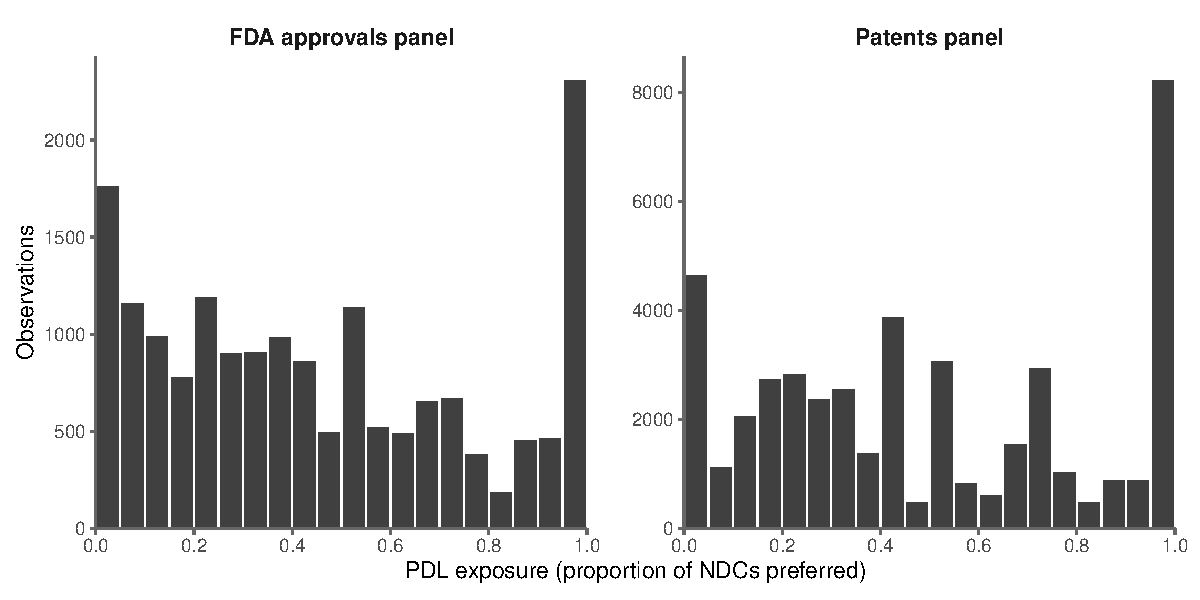
\includegraphics[width=\linewidth]{../output/summary_statistics/pdl_exposure_histogram.pdf}
  \caption{Distribution of PDL exposure in constructed panels}
  \label{fig:pdl_histogram}
\end{figure}

\clearpage

% --- From empirical_results.tex ---

\renewenvironment{table}[1][]{}{}

\subsection{Regression Tables}

\subsubsection{RQ1: Overall Innovation Response}

%TC:ignore
\footnotesize
\begin{table}
\centering
\begin{talltblr}[         %% tabularray outer open
entry=none,label=none,
note{}={* p \num{< 0.05}, ** p \num{< 0.01}, *** p \num{< 0.001}},
]                     %% tabularray outer close
{                     %% tabularray inner open
width=\linewidth,
colspec={Q[]X[]X[]},
column{2,3}={}{halign=c,},
column{1}={}{halign=l,},
hline{32}={1,2,3}{solid, black, 0.05em},
}                     %% tabularray inner close
\toprule
& Patents & FDA Approvals \\ \midrule
2010 × Medicaid Share & \num{-0.041}    & \num{0.215}   \\
                      & (\num{0.038})   & (\num{0.463}) \\
2011 × Medicaid Share & \num{-0.017}    & \num{-0.017}  \\
                      & (\num{0.036})   & (\num{0.381}) \\
2012 × Medicaid Share & \num{0.002}     & \num{0.208}   \\
                      & (\num{0.029})   & (\num{0.412}) \\
2014 × Medicaid Share & \num{-0.022}    & \num{-0.321}  \\
                      & (\num{0.027})   & (\num{0.463}) \\
2015 × Medicaid Share & \num{-0.086}**  & \num{-0.053}  \\
                      & (\num{0.030})   & (\num{0.477}) \\
2016 × Medicaid Share & \num{-0.125}*** & \num{0.414}   \\
                      & (\num{0.034})   & (\num{0.423}) \\
2017 × Medicaid Share & \num{-0.114}**  & \num{1.421}*  \\
                      & (\num{0.036})   & (\num{0.677}) \\
2018 × Medicaid Share & \num{-0.132}*** & \num{0.999}   \\
                      & (\num{0.039})   & (\num{0.550}) \\
2019 × Medicaid Share & \num{-0.189}*** & \num{0.554}   \\
                      & (\num{0.041})   & (\num{0.538}) \\
2020 × Medicaid Share & \num{-0.220}*** & \num{0.732}   \\
                      & (\num{0.043})   & (\num{0.509}) \\
2021 × Medicaid Share & \num{-0.220}*** & \num{0.137}   \\
                      & (\num{0.043})   & (\num{0.632}) \\
2022 × Medicaid Share & \num{-0.233}*** & \num{0.365}   \\
                      & (\num{0.043})   & (\num{0.645}) \\
2023 × Medicaid Share & \num{-0.243}*** & \num{0.846}   \\
                      & (\num{0.044})   & (\num{0.641}) \\
2024 × Medicaid Share & \num{-0.252}*** & \num{0.258}   \\
                      & (\num{0.046})   & (\num{0.523}) \\
2025 × Medicaid Share & \num{-0.228}*** & \num{-0.137}  \\
                      & (\num{0.044})   & (\num{0.510}) \\
Num. obs.             & \num{5281696}   & \num{151200}  \\
R2                    & \num{0.534}     & \num{0.609}   \\
\bottomrule
\end{talltblr}
\end{table}

\captionof{table}{FEOLS event-study estimates: overall innovation response (ex-ante)}
\label{tab:rq1_feols_exante}
\normalsize
%TC:endignore

\clearpage

\subsubsection{RQ2: Medicaid Demand and PDL Exposure}

%TC:ignore
\footnotesize
\begin{table}
\centering
\begin{talltblr}[         %% tabularray outer open
entry=none,label=none,
note{}={* p \num{< 0.05}, ** p \num{< 0.01}, *** p \num{< 0.001}},
]                     %% tabularray outer close
{                     %% tabularray inner open
colspec={Q[]Q[]Q[]Q[]Q[]},
column{2,3,4,5}={}{halign=c,},
column{1}={}{halign=l,},
hline{33}={1,2,3,4,5}{solid, black, 0.05em},
}                     %% tabularray inner close
\toprule
& \SetCell[c=2]{c} Patents && \SetCell[c=2]{c} FDA Approvals & \\
& Medicaid Market Share & PDL Exposure & Medicaid Market Share & PDL Exposure \\ \midrule
2010 & \num{-0.041}    & \num{1.546}     & \num{0.214}   & \num{0.049}   \\
     & (\num{0.038})   & (\num{2.018})   & (\num{0.461}) & (\num{0.807}) \\
2011 & \num{-0.017}    & \num{0.734}     & \num{-0.010}  & \num{-0.243}  \\
     & (\num{0.036})   & (\num{1.642})   & (\num{0.382}) & (\num{0.712}) \\
2012 & \num{0.002}     & \num{1.079}     & \num{0.171}   & \num{1.402}   \\
     & (\num{0.029})   & (\num{1.289})   & (\num{0.406}) & (\num{0.911}) \\
2014 & \num{-0.022}    & \num{4.161}*    & \num{-0.333}  & \num{0.403}   \\
     & (\num{0.026})   & (\num{1.890})   & (\num{0.465}) & (\num{0.647}) \\
2015 & \num{-0.086}**  & \num{0.836}     & \num{-0.088}  & \num{1.163}   \\
     & (\num{0.030})   & (\num{1.480})   & (\num{0.478}) & (\num{0.881}) \\
2016 & \num{-0.126}*** & \num{-1.554}    & \num{0.334}   & \num{2.645}   \\
     & (\num{0.034})   & (\num{1.620})   & (\num{0.426}) & (\num{1.683}) \\
2017 & \num{-0.114}**  & \num{-1.342}    & \num{1.364}*  & \num{1.923}   \\
     & (\num{0.036})   & (\num{1.890})   & (\num{0.680}) & (\num{0.994}) \\
2018 & \num{-0.132}*** & \num{-2.786}    & \num{0.949}   & \num{1.684}   \\
     & (\num{0.039})   & (\num{1.644})   & (\num{0.552}) & (\num{1.021}) \\
2019 & \num{-0.189}*** & \num{-3.806}*   & \num{0.519}   & \num{1.164}*  \\
     & (\num{0.041})   & (\num{1.912})   & (\num{0.539}) & (\num{0.592}) \\
2020 & \num{-0.220}*** & \num{-4.649}*   & \num{0.687}   & \num{1.579}   \\
     & (\num{0.043})   & (\num{1.894})   & (\num{0.514}) & (\num{0.942}) \\
2021 & \num{-0.220}*** & \num{-5.266}**  & \num{0.038}   & \num{3.114}*  \\
     & (\num{0.043})   & (\num{1.687})   & (\num{0.640}) & (\num{1.394}) \\
2022 & \num{-0.233}*** & \num{-6.029}**  & \num{0.333}   & \num{0.994}   \\
     & (\num{0.044})   & (\num{1.941})   & (\num{0.648}) & (\num{0.655}) \\
2023 & \num{-0.243}*** & \num{-6.925}*** & \num{0.809}   & \num{1.185}   \\
     & (\num{0.044})   & (\num{1.851})   & (\num{0.649}) & (\num{1.738}) \\
2024 & \num{-0.252}*** & \num{-6.484}*** & \num{0.272}   & \num{-0.452}  \\
     & (\num{0.046})   & (\num{1.788})   & (\num{0.523}) & (\num{0.590}) \\
2025 & \num{-0.227}*** & \num{-4.588}**  & \num{-0.109}  & \num{-1.118}  \\
     & (\num{0.044})   & (\num{1.549})   & (\num{0.506}) & (\num{0.908}) \\
Num. obs. & \SetCell[c=2]{c} \num{5281696} && \SetCell[c=2]{c} \num{151200} & \\
R2        & \SetCell[c=2]{c} \num{0.535}   && \SetCell[c=2]{c} \num{0.609}  & \\
\bottomrule
\end{talltblr}
\end{table}

\captionof{table}{FEOLS event-study estimates: Medicaid demand and PDL exposure (ex-ante)}
\label{tab:rq2_feols_exante}
\normalsize
%TC:endignore

\clearpage

\subsection{Therapeutic-Class Substitutability}

%TC:ignore
\makeatletter
\renewenvironment{table}[1][H]{\@float{table}[H]}{\end@float}
\makeatother
\begin{table}[!h]
\centering
\caption{\label{tab:class_substitutability}Average annual distinct NDC count by ATC class}
\centering
\begin{tabular}[t]{llr}
\toprule
ATC & Therapeutic class & Mean annual $n_c$\\
\midrule
N & Nervous system & 7351\\
C & Cardiovascular system & 4297\\
A & Alimentary tract and metabolism & 3407\\
J & Anti-infectives for systemic use & 2332\\
D & Dermatologicals & 1771\\
\addlinespace
R & Respiratory system & 1672\\
M & Musculo-skeletal system & 1407\\
B & Blood and blood-forming organs & 1389\\
L & Antineoplastic and immunomodulating & 932\\
G & Genito-urinary and sex hormones & 906\\
\addlinespace
H & Systemic hormonal preparations & 768\\
S & Sensory organs & 579\\
V & Various & 211\\
P & Antiparasitic products & 165\\
\bottomrule
\end{tabular}
\end{table}

\renewenvironment{table}[1][]{}{}
%TC:endignore

\clearpage

% --- From robustness.tex ---

\subsection{Robustness Regression Tables}

\subsubsection{RQ1: Ex-Post FEOLS}

%TC:ignore
\footnotesize
\begin{table}
\centering
\begin{talltblr}[         %% tabularray outer open
entry=none,label=none,
note{}={* p \num{< 0.05}, ** p \num{< 0.01}, *** p \num{< 0.001}},
]                     %% tabularray outer close
{                     %% tabularray inner open
width=\linewidth,
colspec={Q[]X[]X[]},
column{2,3}={}{halign=c,},
column{1}={}{halign=l,},
hline{32}={1,2,3}{solid, black, 0.05em},
}                     %% tabularray inner close
\toprule
& Patents & FDA Approvals \\ \midrule
2010 × Medicaid Share & \num{-0.033}    & \num{0.286}   \\
                      & (\num{0.035})   & (\num{0.450}) \\
2011 × Medicaid Share & \num{-0.010}    & \num{0.336}   \\
                      & (\num{0.033})   & (\num{0.413}) \\
2012 × Medicaid Share & \num{0.004}     & \num{0.414}   \\
                      & (\num{0.027})   & (\num{0.455}) \\
2014 × Medicaid Share & \num{-0.018}    & \num{-0.324}  \\
                      & (\num{0.024})   & (\num{0.533}) \\
2015 × Medicaid Share & \num{-0.088}**  & \num{0.005}   \\
                      & (\num{0.027})   & (\num{0.420}) \\
2016 × Medicaid Share & \num{-0.123}*** & \num{0.550}   \\
                      & (\num{0.032})   & (\num{0.413}) \\
2017 × Medicaid Share & \num{-0.122}*** & \num{1.635}*  \\
                      & (\num{0.034})   & (\num{0.688}) \\
2018 × Medicaid Share & \num{-0.135}*** & \num{1.240}*  \\
                      & (\num{0.037})   & (\num{0.560}) \\
2019 × Medicaid Share & \num{-0.194}*** & \num{0.400}   \\
                      & (\num{0.039})   & (\num{0.497}) \\
2020 × Medicaid Share & \num{-0.225}*** & \num{0.652}   \\
                      & (\num{0.041})   & (\num{0.529}) \\
2021 × Medicaid Share & \num{-0.222}*** & \num{0.218}   \\
                      & (\num{0.040})   & (\num{0.573}) \\
2022 × Medicaid Share & \num{-0.233}*** & \num{0.418}   \\
                      & (\num{0.040})   & (\num{0.590}) \\
2023 × Medicaid Share & \num{-0.238}*** & \num{0.842}   \\
                      & (\num{0.040})   & (\num{0.576}) \\
2024 × Medicaid Share & \num{-0.250}*** & \num{0.137}   \\
                      & (\num{0.042})   & (\num{0.502}) \\
2025 × Medicaid Share & \num{-0.212}*** & \num{-0.380}  \\
                      & (\num{0.041})   & (\num{0.531}) \\
Num. obs.             & \num{5281696}   & \num{151200}  \\
R2                    & \num{0.534}     & \num{0.609}   \\
\bottomrule
\end{talltblr}
\end{table}

\captionof{table}{FEOLS event-study estimates: overall innovation response (ex-post)}
\label{tab:rob_rq1_feols_expost}
\normalsize
%TC:endignore

\begin{figure}[!h]
  \centering
  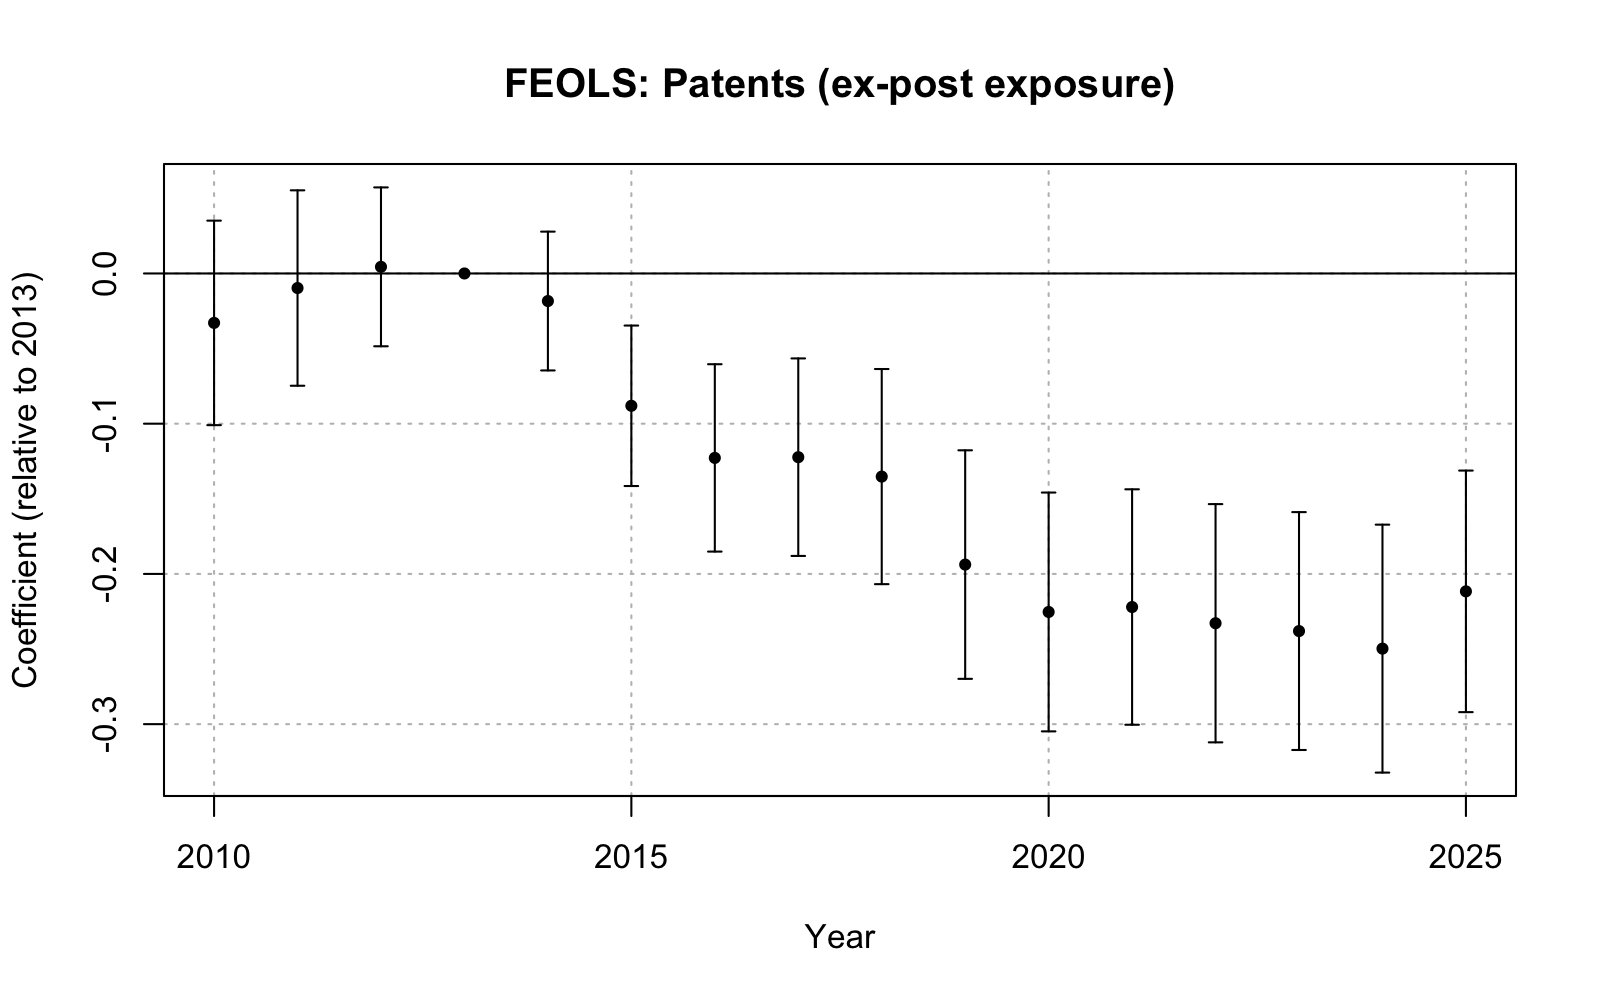
\includegraphics[width=\linewidth]{../output/RQ1/patent_feols_expost.png}
  \caption{FEOLS event study: patents, ex-post Medicaid exposure}
  \label{fig:rob_rq1_patent_feols_expost}
\end{figure}

\begin{figure}[!h]
  \centering
  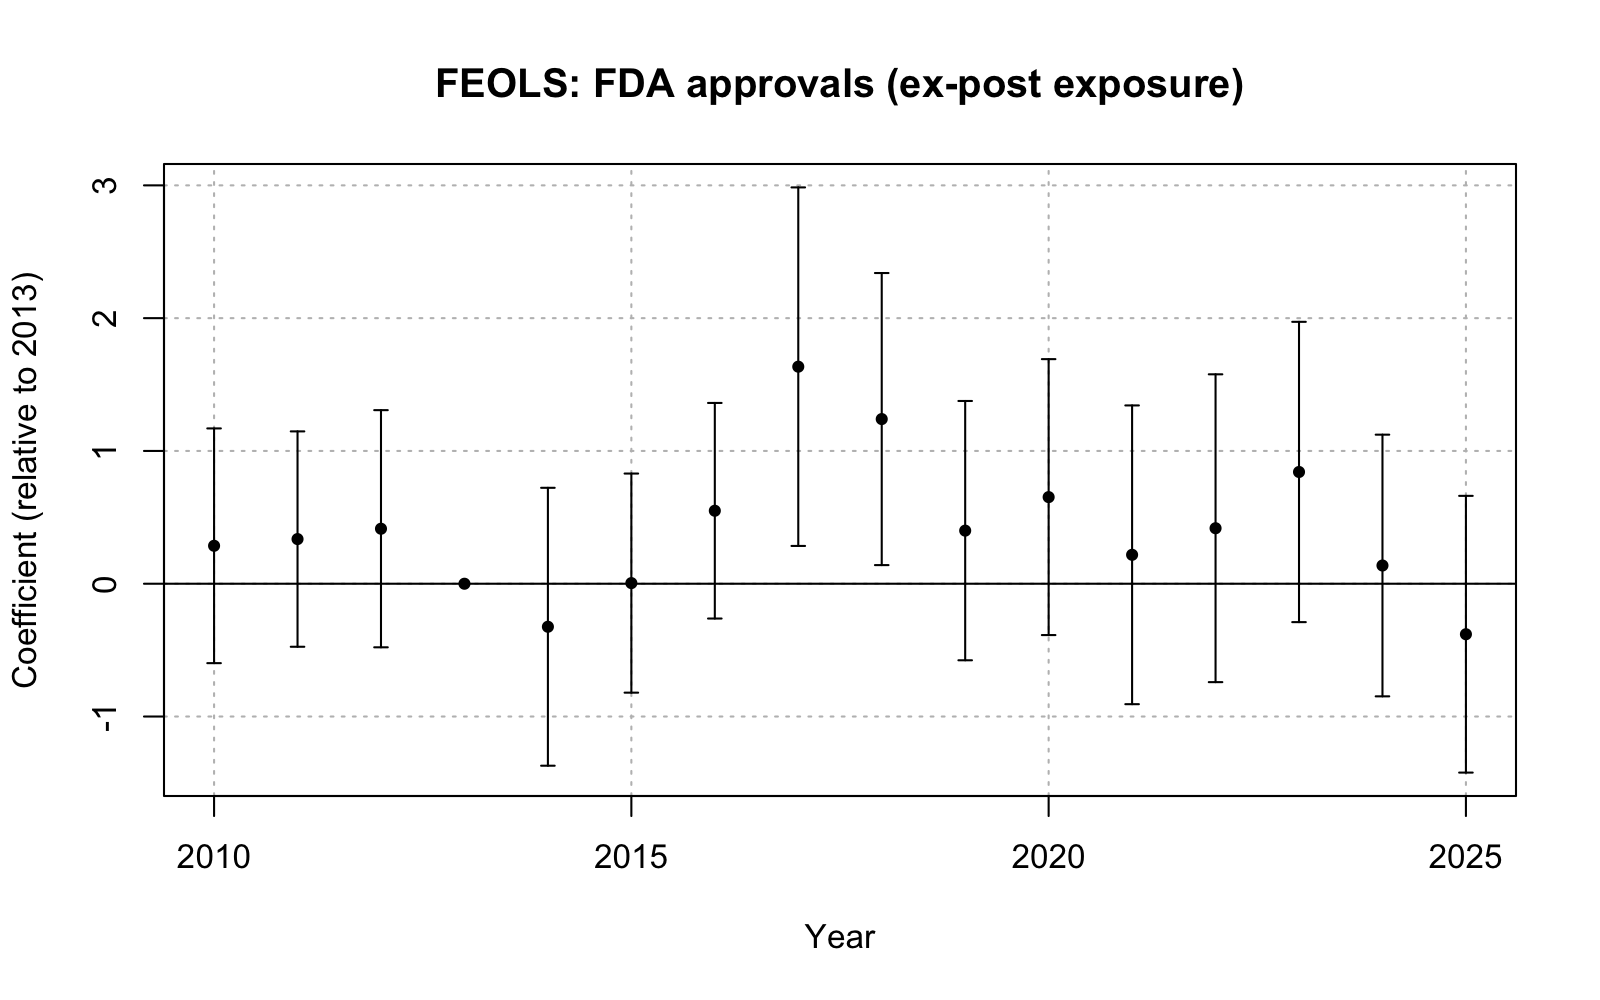
\includegraphics[width=\linewidth]{../output/RQ1/fda_feols_expost.png}
  \caption{FEOLS event study: FDA approvals, ex-post Medicaid exposure}
  \label{fig:rob_rq1_fda_feols_expost}
\end{figure}

\clearpage

\subsubsection{RQ1: Ex-Ante FE Poisson}

%TC:ignore
\footnotesize
\begin{table}
\centering
\begin{talltblr}[         %% tabularray outer open
entry=none,label=none,
note{}={* p \num{< 0.05}, ** p \num{< 0.01}, *** p \num{< 0.001}},
]                     %% tabularray outer close
{                     %% tabularray inner open
width=\linewidth,
colspec={Q[]X[]X[]},
column{2,3}={}{halign=c,},
column{1}={}{halign=l,},
hline{32}={1,2,3}{solid, black, 0.05em},
}                     %% tabularray inner close
\toprule
& Patents & FDA Approvals \\ \midrule
2010 × Medicaid Share & \num{0.120}     & \num{0.237}   \\
                      & (\num{0.154})   & (\num{0.636}) \\
2011 × Medicaid Share & \num{0.218}     & \num{0.326}   \\
                      & (\num{0.140})   & (\num{0.446}) \\
2012 × Medicaid Share & \num{0.115}     & \num{0.643}   \\
                      & (\num{0.108})   & (\num{0.615}) \\
2014 × Medicaid Share & \num{-0.092}    & \num{-0.545}  \\
                      & (\num{0.108})   & (\num{0.638}) \\
2015 × Medicaid Share & \num{-0.300}*   & \num{-0.434}  \\
                      & (\num{0.118})   & (\num{0.632}) \\
2016 × Medicaid Share & \num{-0.435}*** & \num{-0.834}  \\
                      & (\num{0.124})   & (\num{0.478}) \\
2017 × Medicaid Share & \num{-0.397}**  & \num{-0.495}  \\
                      & (\num{0.131})   & (\num{0.480}) \\
2018 × Medicaid Share & \num{-0.415}**  & \num{-0.772}  \\
                      & (\num{0.149})   & (\num{0.530}) \\
2019 × Medicaid Share & \num{-0.784}*** & \num{-0.381}  \\
                      & (\num{0.154})   & (\num{0.565}) \\
2020 × Medicaid Share & \num{-0.998}*** & \num{-0.733}  \\
                      & (\num{0.173})   & (\num{0.574}) \\
2021 × Medicaid Share & \num{-0.989}*** & \num{-0.867}  \\
                      & (\num{0.170})   & (\num{0.729}) \\
2022 × Medicaid Share & \num{-1.137}*** & \num{-0.637}  \\
                      & (\num{0.186})   & (\num{0.594}) \\
2023 × Medicaid Share & \num{-1.324}*** & \num{-0.566}  \\
                      & (\num{0.201})   & (\num{0.511}) \\
2024 × Medicaid Share & \num{-1.474}*** & \num{-0.680}  \\
                      & (\num{0.261})   & (\num{0.573}) \\
2025 × Medicaid Share & \num{-1.110}*** & \num{-0.668}  \\
                      & (\num{0.229})   & (\num{0.580}) \\
Num. obs.             & \num{1300944}   & \num{42176}   \\
\bottomrule
\end{talltblr}
\end{table}

\captionof{table}{FE Poisson event-study estimates: overall innovation response (ex-ante)}
\label{tab:rob_rq1_fepois_exante}
\normalsize
%TC:endignore

\begin{figure}[!h]
  \centering
  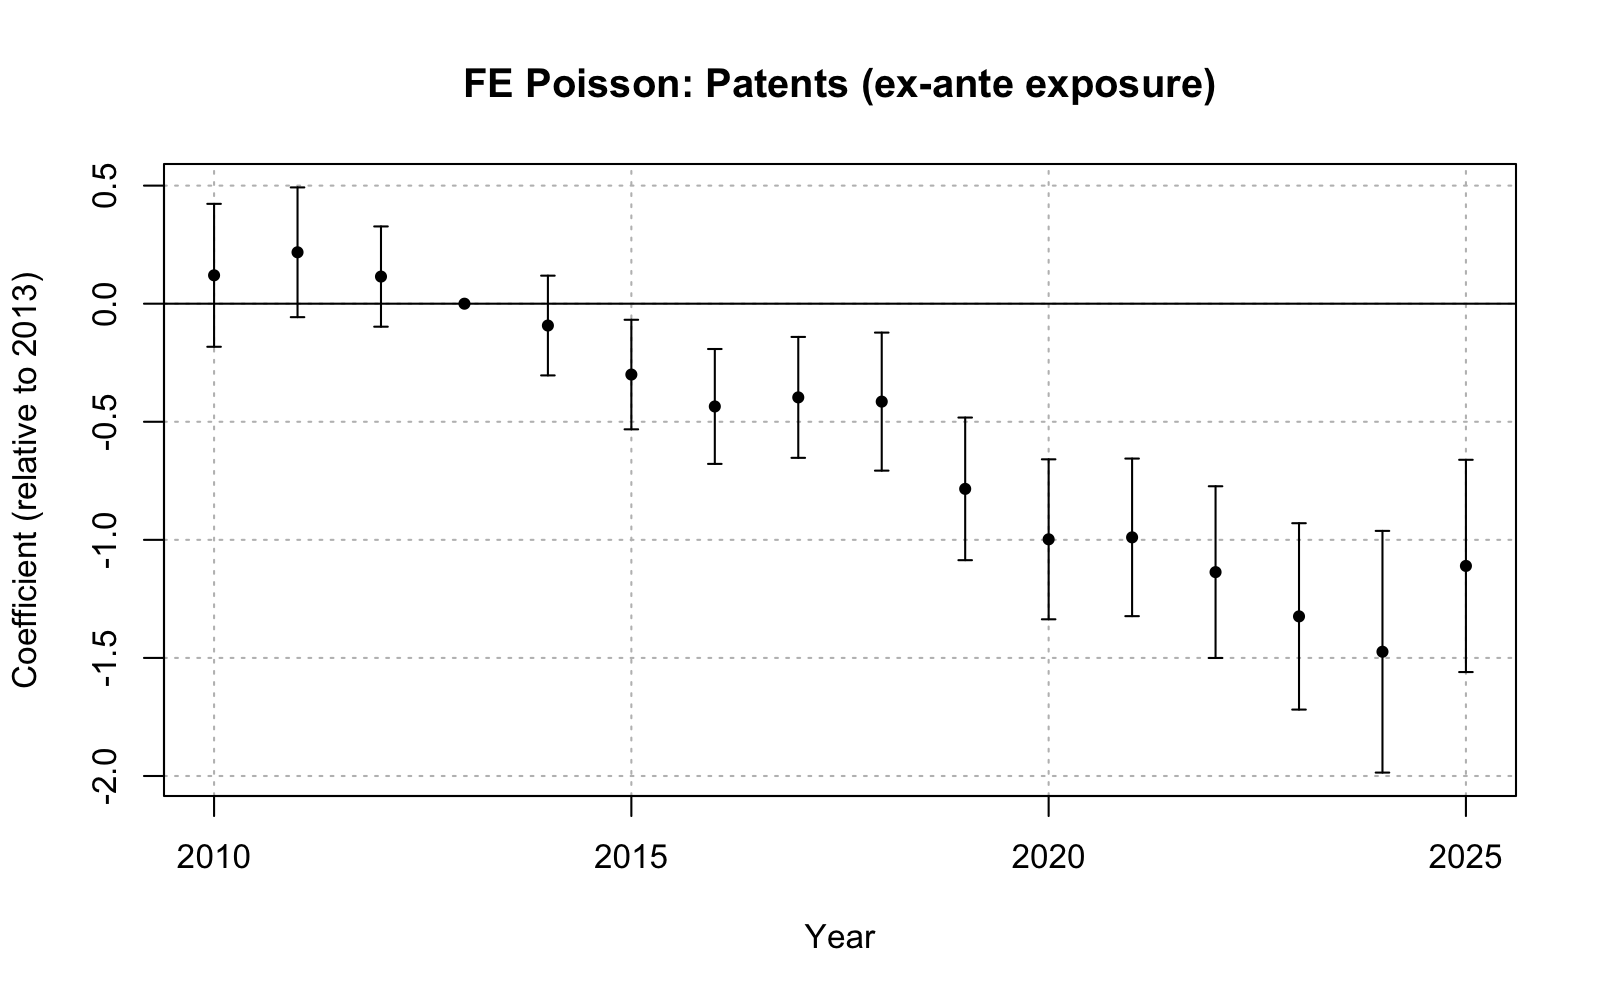
\includegraphics[width=\linewidth]{../output/RQ1/patent_poi_exante.png}
  \caption{FE Poisson event study: patents, ex-ante Medicaid exposure}
  \label{fig:rob_rq1_patent_poi_exante}
\end{figure}

\begin{figure}[!h]
  \centering
  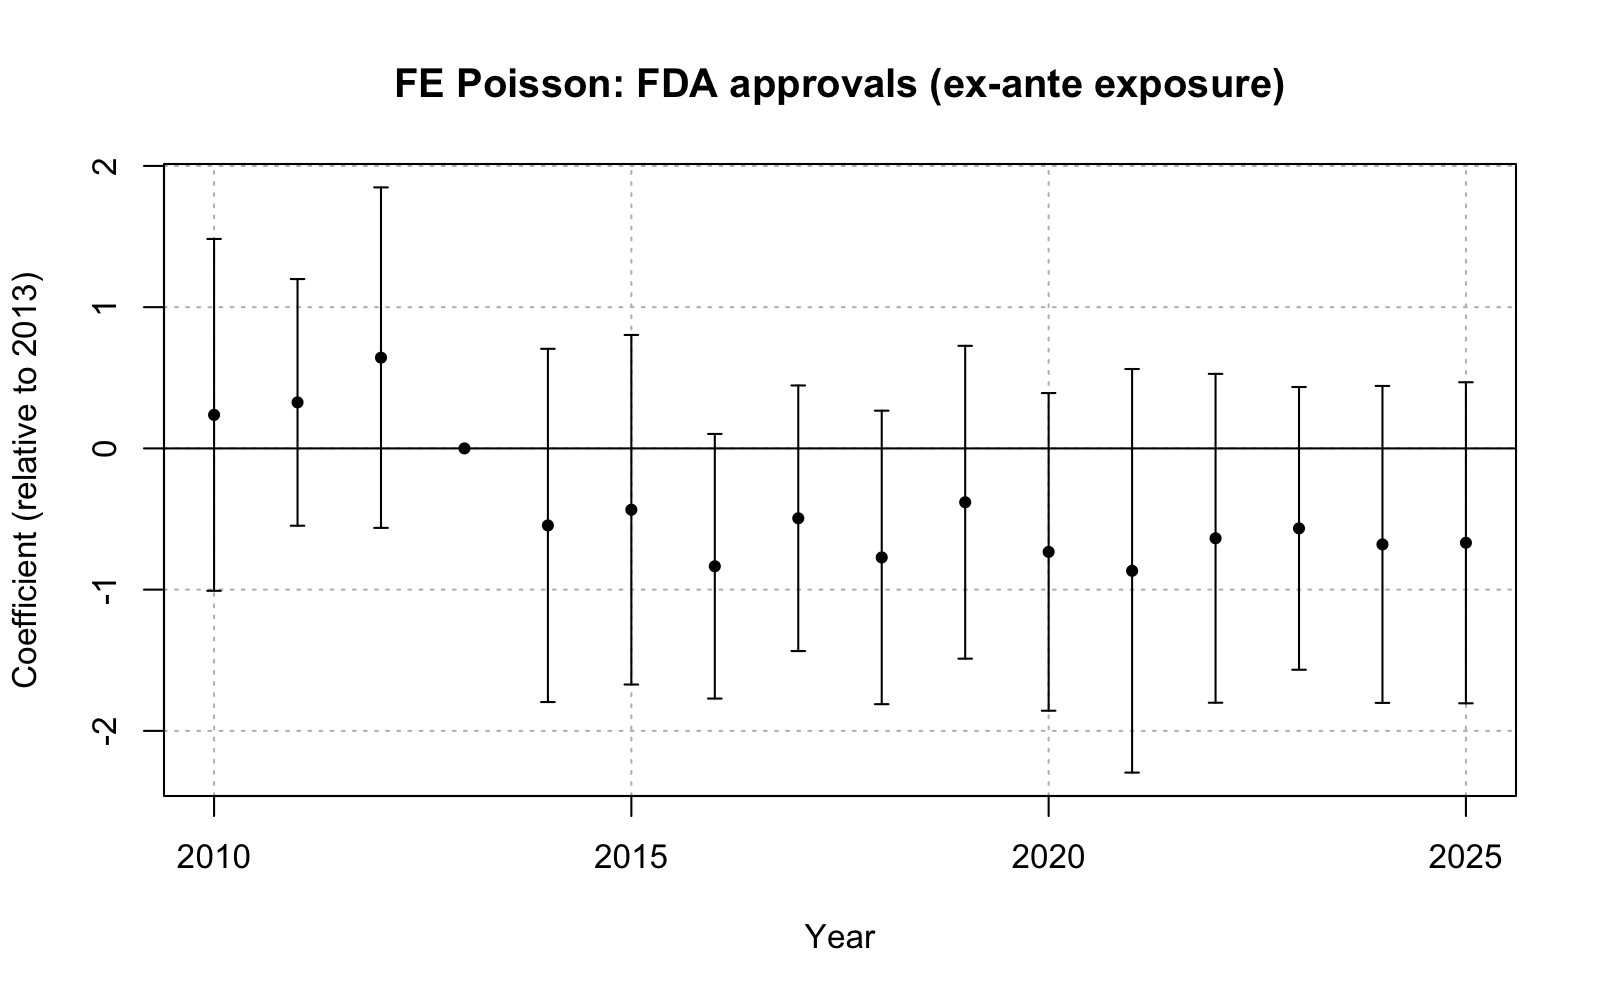
\includegraphics[width=\linewidth]{../output/RQ1/fda_poi_exante.png}
  \caption{FE Poisson event study: FDA approvals, ex-ante Medicaid exposure}
  \label{fig:rob_rq1_fda_poi_exante}
\end{figure}

\clearpage

\subsubsection{RQ1: Ex-Post FE Poisson}

%TC:ignore
\footnotesize
\begin{table}
\centering
\begin{talltblr}[         %% tabularray outer open
entry=none,label=none,
note{}={* p \num{< 0.05}, ** p \num{< 0.01}, *** p \num{< 0.001}},
]                     %% tabularray outer close
{                     %% tabularray inner open
width=\linewidth,
colspec={Q[]X[]X[]},
column{2,3}={}{halign=c,},
column{1}={}{halign=l,},
hline{32}={1,2,3}{solid, black, 0.05em},
}                     %% tabularray inner close
\toprule
& Patents & FDA Approvals \\ \midrule
2010 × Medicaid Share & \num{0.129}     & \num{0.453}   \\
                      & (\num{0.157})   & (\num{0.869}) \\
2011 × Medicaid Share & \num{0.240}     & \num{1.138}   \\
                      & (\num{0.145})   & (\num{0.687}) \\
2012 × Medicaid Share & \num{0.124}     & \num{1.250}   \\
                      & (\num{0.115})   & (\num{0.863}) \\
2014 × Medicaid Share & \num{-0.086}    & \num{-0.711}  \\
                      & (\num{0.106})   & (\num{0.996}) \\
2015 × Medicaid Share & \num{-0.367}**  & \num{-0.431}  \\
                      & (\num{0.119})   & (\num{0.725}) \\
2016 × Medicaid Share & \num{-0.515}*** & \num{-0.788}  \\
                      & (\num{0.129})   & (\num{0.660}) \\
2017 × Medicaid Share & \num{-0.533}*** & \num{-0.278}  \\
                      & (\num{0.134})   & (\num{0.735}) \\
2018 × Medicaid Share & \num{-0.556}*** & \num{-0.595}  \\
                      & (\num{0.157})   & (\num{0.713}) \\
2019 × Medicaid Share & \num{-0.998}*** & \num{-0.625}  \\
                      & (\num{0.167})   & (\num{0.764}) \\
2020 × Medicaid Share & \num{-1.293}*** & \num{-0.916}  \\
                      & (\num{0.190})   & (\num{0.839}) \\
2021 × Medicaid Share & \num{-1.313}*** & \num{-0.909}  \\
                      & (\num{0.188})   & (\num{0.910}) \\
2022 × Medicaid Share & \num{-1.564}*** & \num{-0.657}  \\
                      & (\num{0.203})   & (\num{0.775}) \\
2023 × Medicaid Share & \num{-1.803}*** & \num{-0.618}  \\
                      & (\num{0.224})   & (\num{0.695}) \\
2024 × Medicaid Share & \num{-2.021}*** & \num{-0.969}  \\
                      & (\num{0.266})   & (\num{0.854}) \\
2025 × Medicaid Share & \num{-1.692}*** & \num{-1.254}  \\
                      & (\num{0.262})   & (\num{0.892}) \\
Num. obs.             & \num{1300944}   & \num{42176}   \\
\bottomrule
\end{talltblr}
\end{table}

\captionof{table}{FE Poisson event-study estimates: overall innovation response (ex-post)}
\label{tab:rob_rq1_fepois_expost}
\normalsize
%TC:endignore

\begin{figure}[!h]
  \centering
  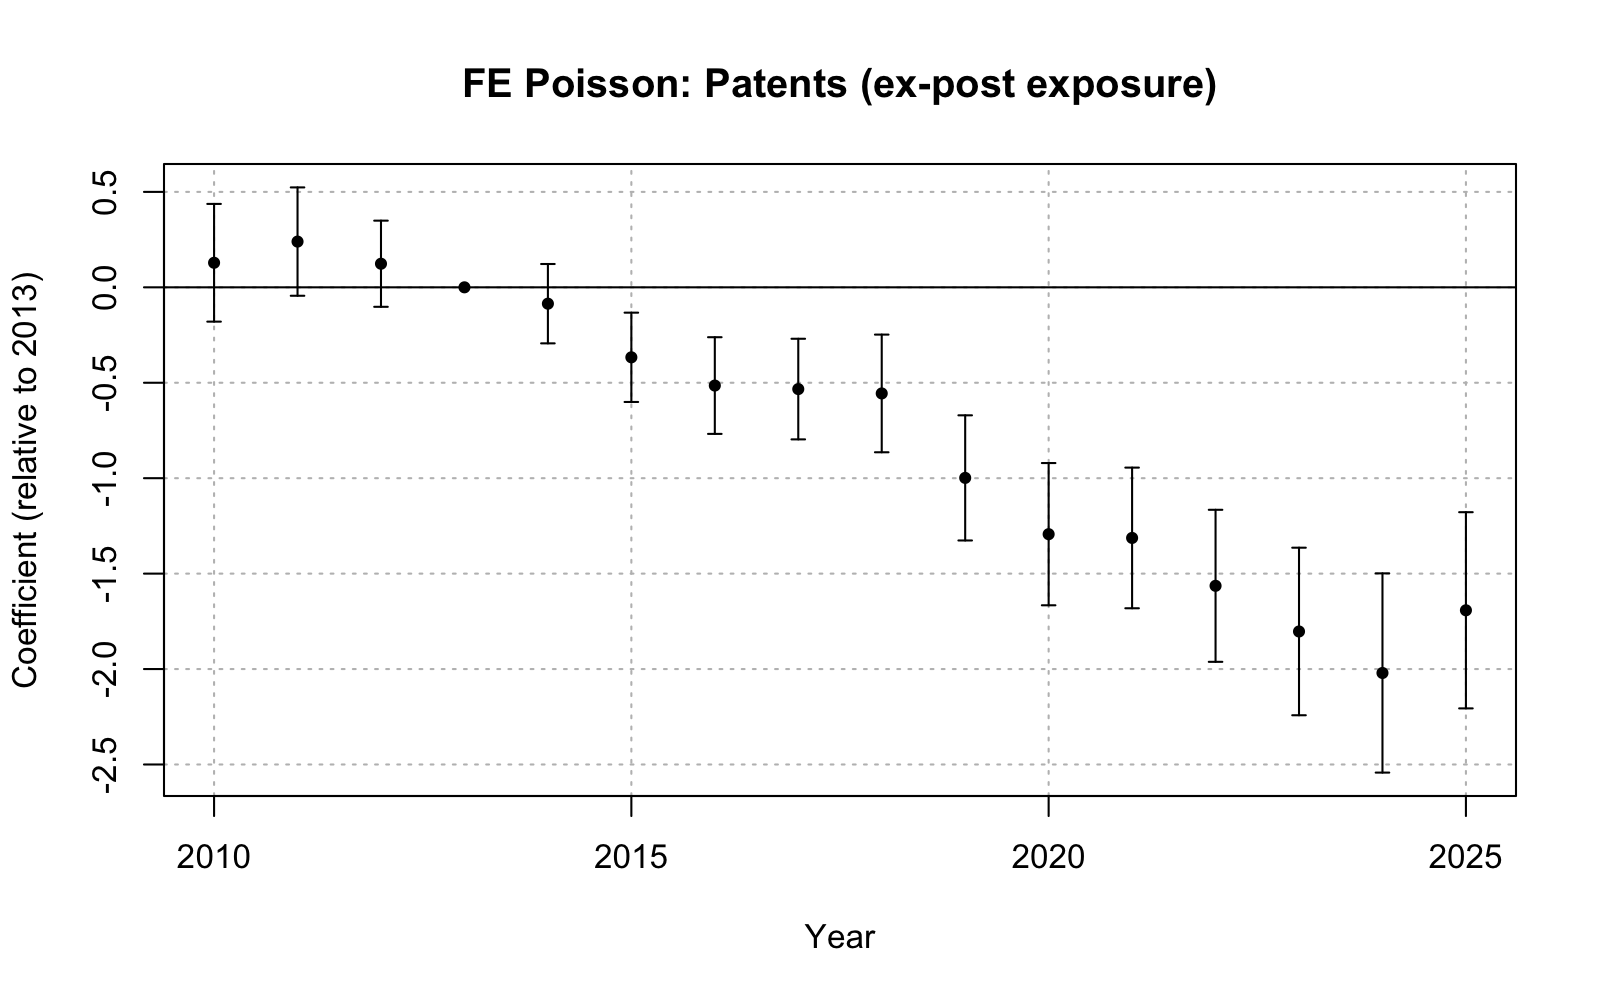
\includegraphics[width=\linewidth]{../output/RQ1/patent_poi_expost.png}
  \caption{FE Poisson event study: patents, ex-post Medicaid exposure}
  \label{fig:rob_rq1_patent_poi_expost}
\end{figure}

\begin{figure}[!h]
  \centering
  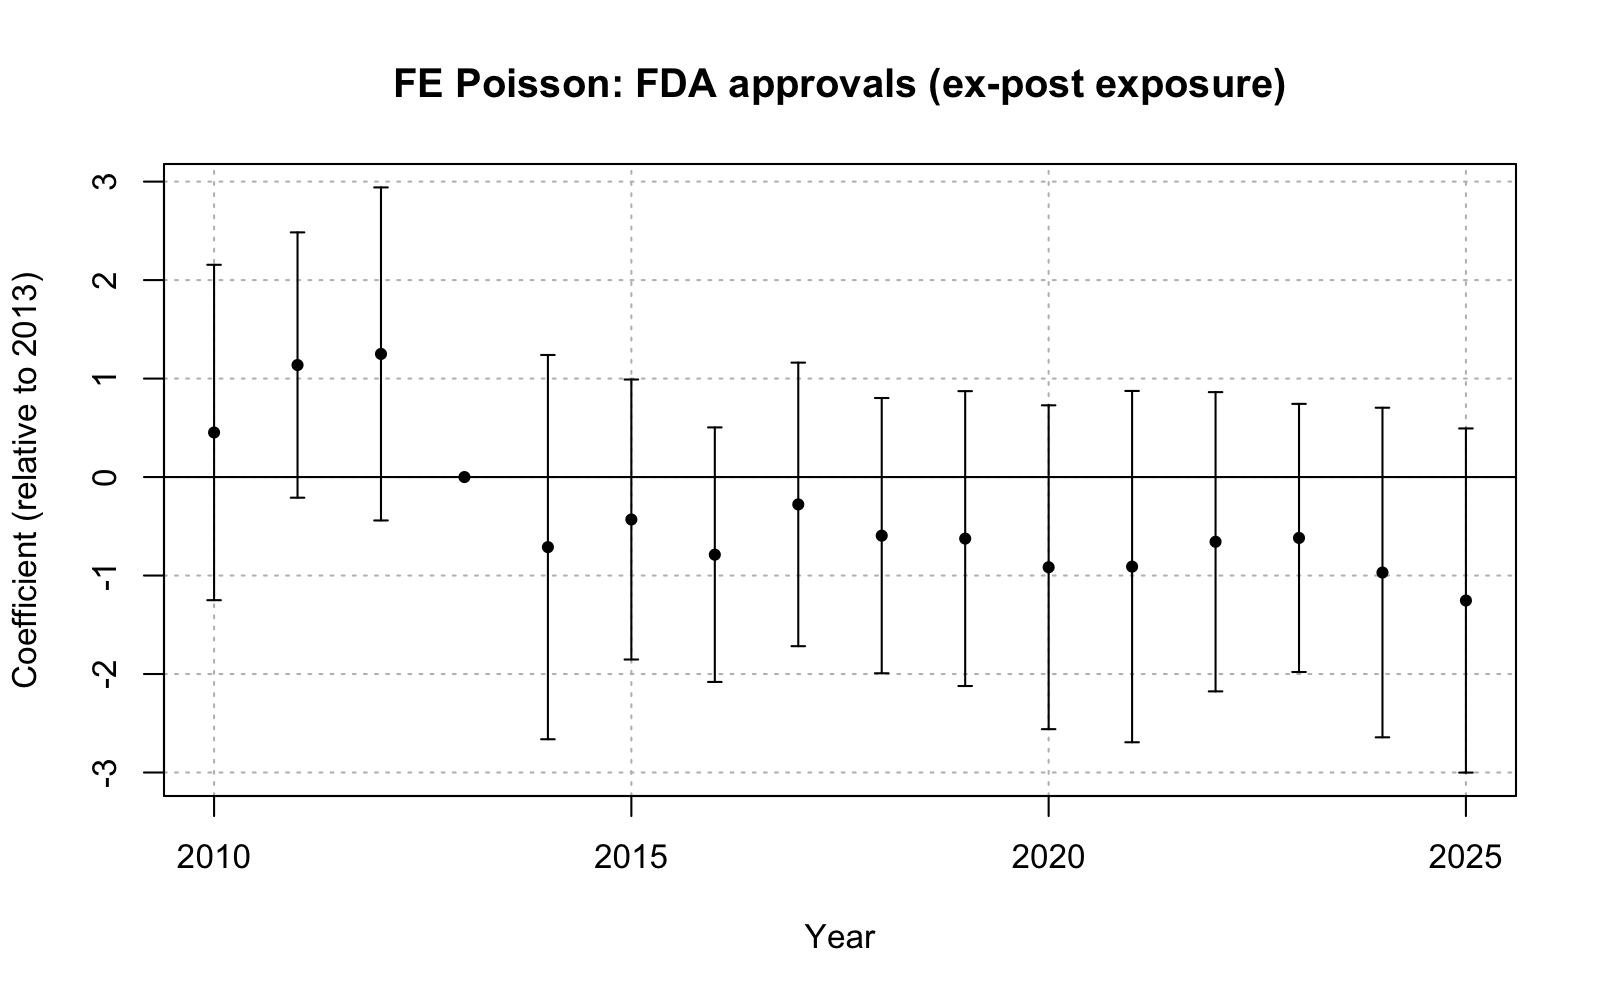
\includegraphics[width=\linewidth]{../output/RQ1/fda_poi_expost.png}
  \caption{FE Poisson event study: FDA approvals, ex-post Medicaid exposure}
  \label{fig:rob_rq1_fda_poi_expost}
\end{figure}

\clearpage

\subsubsection{RQ1: Binned Treatment}

%TC:ignore
\makeatletter
\renewenvironment{table}[1][H]{\@float{table}[H]}{\end@float}
\makeatother
\begin{table}[htbp]
\centering
\caption{Pre-expansion Medicaid market shares and bin assignments}
\label{tab:atc_bins}
\begin{tabular}{llrl}
\toprule
\multicolumn{1}{c}{ATC} & \multicolumn{1}{c}{Therapeutic Area} & \multicolumn{1}{c}{Medicaid Share} & \multicolumn{1}{c}{Bin} \\
\midrule
N & Nervous system                  & 0.363 & High   \\
C & Cardiovascular system           & 0.215 & High   \\
J & Anti-infectives for systemic use & 0.120 & Medium \\
D & Dermatologicals                 & 0.099 & Medium \\
R & Respiratory system              & 0.085 & Low    \\
A & Alimentary tract and metabolism & 0.068 & Low    \\
M & Musculo-skeletal system         & 0.015 & Low    \\
H & Systemic hormonal preparations  & 0.012 & Low    \\
L & Antineoplastic and immunomodulating agents & 0.006 & Low \\
G & Genito-urinary system and sex hormones     & 0.006 & Low \\
S & Sensory organs                  & 0.005 & Low    \\
B & Blood and blood-forming organs  & 0.005 & Low    \\
V & Various                         & 0.000 & Low    \\
P & Antiparasitic products          & 0.000 & Low    \\
\bottomrule
\end{tabular}
\end{table}

\renewenvironment{table}[1][]{}{}
%TC:endignore

%TC:ignore
\footnotesize
\begin{table}
\centering
\begin{talltblr}[         %% tabularray outer open
entry=none,label=none,
note{}={* p \num{< 0.05}, ** p \num{< 0.01}, *** p \num{< 0.001}},
]                     %% tabularray outer close
{                     %% tabularray inner open
width=\linewidth,
colspec={Q[]X[]X[]X[]X[]},
column{2,3,4,5}={}{halign=c,},
column{1}={}{halign=l,},
hline{33}={1,2,3,4,5}{solid, black, 0.05em},
}                     %% tabularray inner close
\toprule
& \SetCell[c=2]{c} Patents && \SetCell[c=2]{c} FDA Approvals & \\
& Medium Bin & High Bin & Medium Bin & High Bin \\ \midrule
2010 & \num{-0.008}    & \num{-0.029}    & \num{0.042}   & \num{0.085}   \\
     & (\num{0.006})   & (\num{0.017})   & (\num{0.055}) & (\num{0.140}) \\
2011 & \num{-0.005}    & \num{-0.025}    & \num{0.058}   & \num{-0.064}  \\
     & (\num{0.006})   & (\num{0.016})   & (\num{0.065}) & (\num{0.105}) \\
2012 & \num{0.009}     & \num{-0.003}    & \num{0.042}   & \num{0.033}   \\
     & (\num{0.006})   & (\num{0.012})   & (\num{0.077}) & (\num{0.121}) \\
2014 & \num{0.015}**   & \num{-0.002}    & \num{0.047}   & \num{-0.091}  \\
     & (\num{0.005})   & (\num{0.011})   & (\num{0.067}) & (\num{0.130}) \\
2015 & \num{0.002}     & \num{-0.027}*   & \num{0.006}   & \num{-0.005}  \\
     & (\num{0.005})   & (\num{0.013})   & (\num{0.073}) & (\num{0.148}) \\
2016 & \num{0.007}     & \num{-0.058}*** & \num{0.158}   & \num{0.070}   \\
     & (\num{0.006})   & (\num{0.014})   & (\num{0.101}) & (\num{0.130}) \\
2017 & \num{0.005}     & \num{-0.047}**  & \num{0.239}*  & \num{0.326}   \\
     & (\num{0.006})   & (\num{0.015})   & (\num{0.114}) & (\num{0.181}) \\
2018 & \num{-0.009}    & \num{-0.075}*** & \num{0.185}*  & \num{0.213}   \\
     & (\num{0.006})   & (\num{0.017})   & (\num{0.093}) & (\num{0.155}) \\
2019 & \num{-0.004}    & \num{-0.092}*** & \num{0.071}   & \num{0.206}   \\
     & (\num{0.007})   & (\num{0.017})   & (\num{0.077}) & (\num{0.162}) \\
2020 & \num{-0.003}    & \num{-0.108}*** & \num{0.012}   & \num{0.141}   \\
     & (\num{0.006})   & (\num{0.018})   & (\num{0.092}) & (\num{0.142}) \\
2021 & \num{-0.005}    & \num{-0.118}*** & \num{0.127}   & \num{-0.048}  \\
     & (\num{0.006})   & (\num{0.018})   & (\num{0.105}) & (\num{0.182}) \\
2022 & \num{-0.010}    & \num{-0.129}*** & \num{0.101}   & \num{0.040}   \\
     & (\num{0.006})   & (\num{0.018})   & (\num{0.075}) & (\num{0.184}) \\
2023 & \num{-0.011}    & \num{-0.141}*** & \num{0.152}   & \num{0.154}   \\
     & (\num{0.006})   & (\num{0.019})   & (\num{0.087}) & (\num{0.182}) \\
2024 & \num{-0.005}    & \num{-0.142}*** & \num{0.037}   & \num{0.070}   \\
     & (\num{0.010})   & (\num{0.019})   & (\num{0.066}) & (\num{0.146}) \\
2025 & \num{-0.020}**  & \num{-0.155}*** & \num{0.010}   & \num{0.032}   \\
     & (\num{0.006})   & (\num{0.019})   & (\num{0.067}) & (\num{0.153}) \\
Num. obs. & \SetCell[c=2]{c} \num{5281696} && \SetCell[c=2]{c} \num{151200} & \\
R2        & \SetCell[c=2]{c} \num{0.534}   && \SetCell[c=2]{c} \num{0.609}  & \\
\bottomrule
\end{talltblr}
\end{table}

\captionof{table}{Binned treatment event-study estimates (FEOLS, ex-ante)}
\label{tab:rob_binned}
\normalsize
%TC:endignore

\begin{figure}[!h]
  \centering
  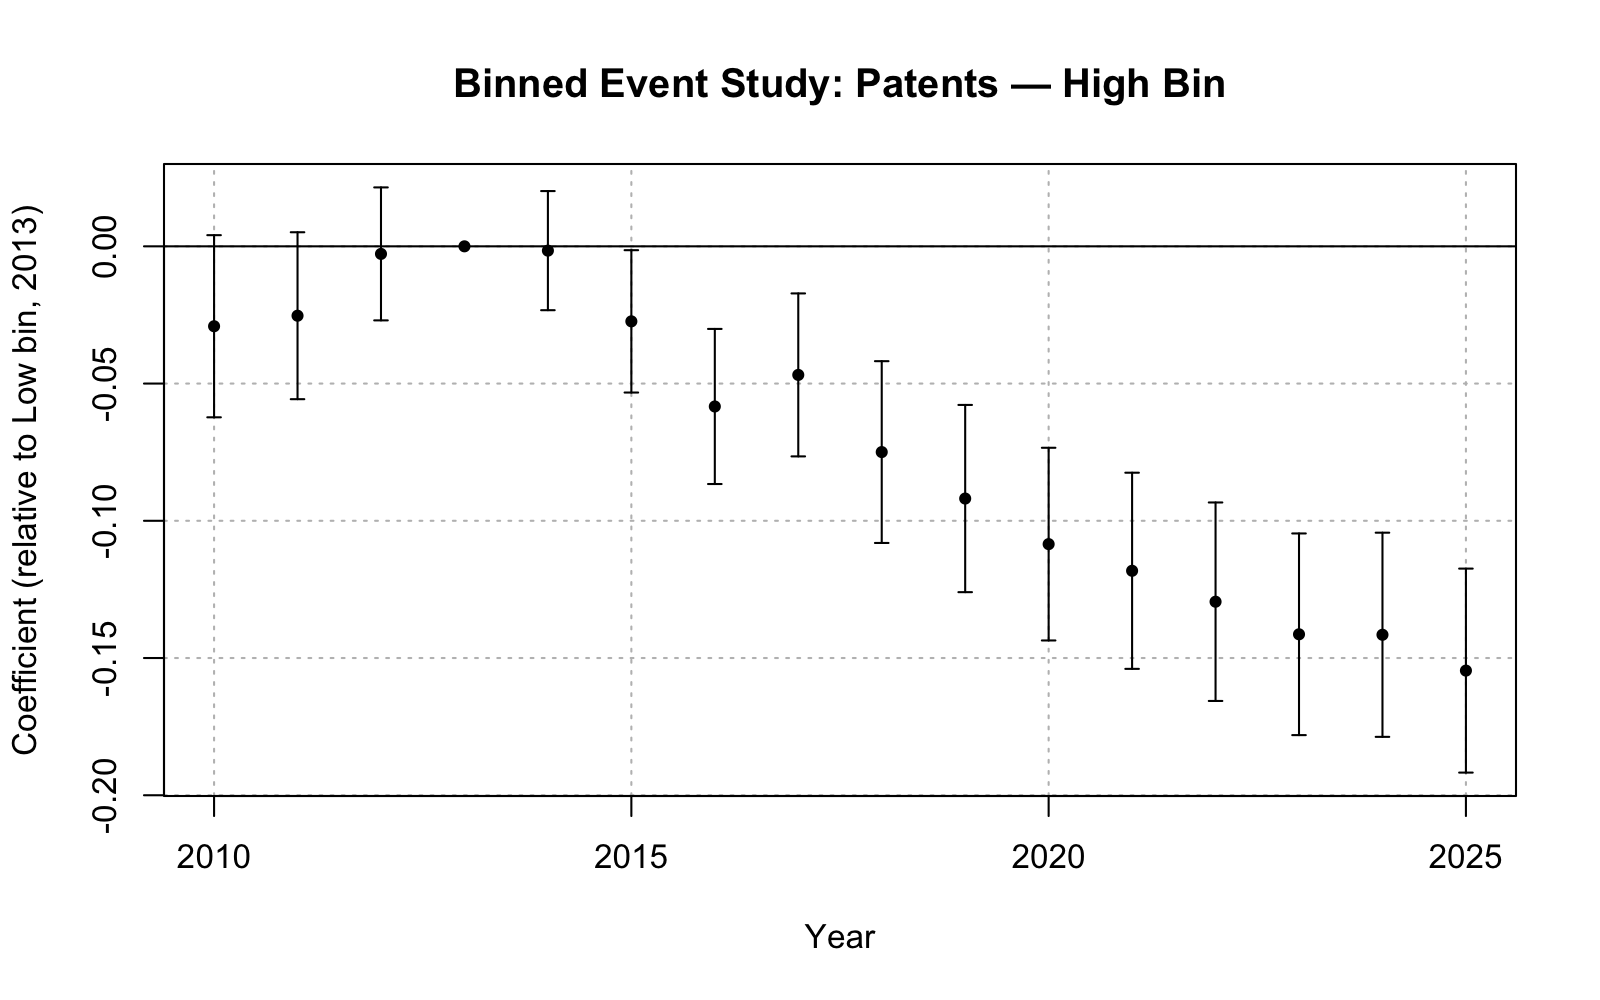
\includegraphics[width=\linewidth]{../output/robustness/binned_treatment/binned_patent_high_es.png}
  \caption{Binned event study: patents, high-exposure bin (N, C)}
  \label{fig:rob_binned_patent_high}
\end{figure}

\begin{figure}[!h]
  \centering
  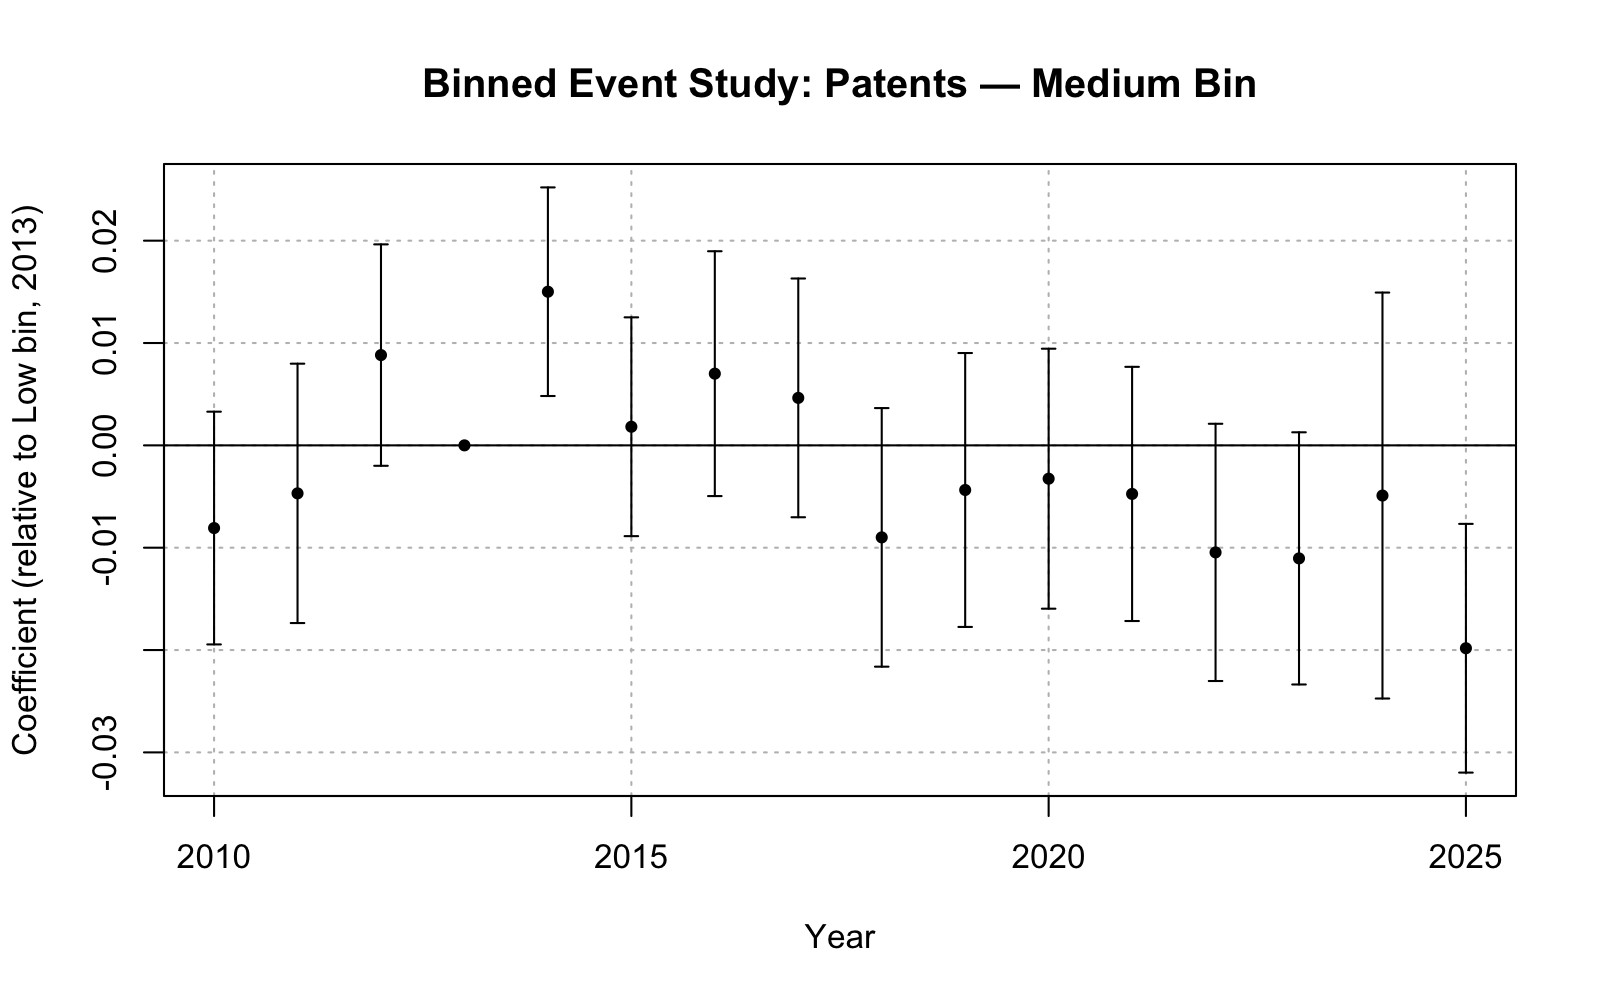
\includegraphics[width=\linewidth]{../output/robustness/binned_treatment/binned_patent_medium_es.png}
  \caption{Binned event study: patents, medium-exposure bin (J, D)}
  \label{fig:rob_binned_patent_medium}
\end{figure}

\clearpage

\begin{figure}[!h]
  \centering
  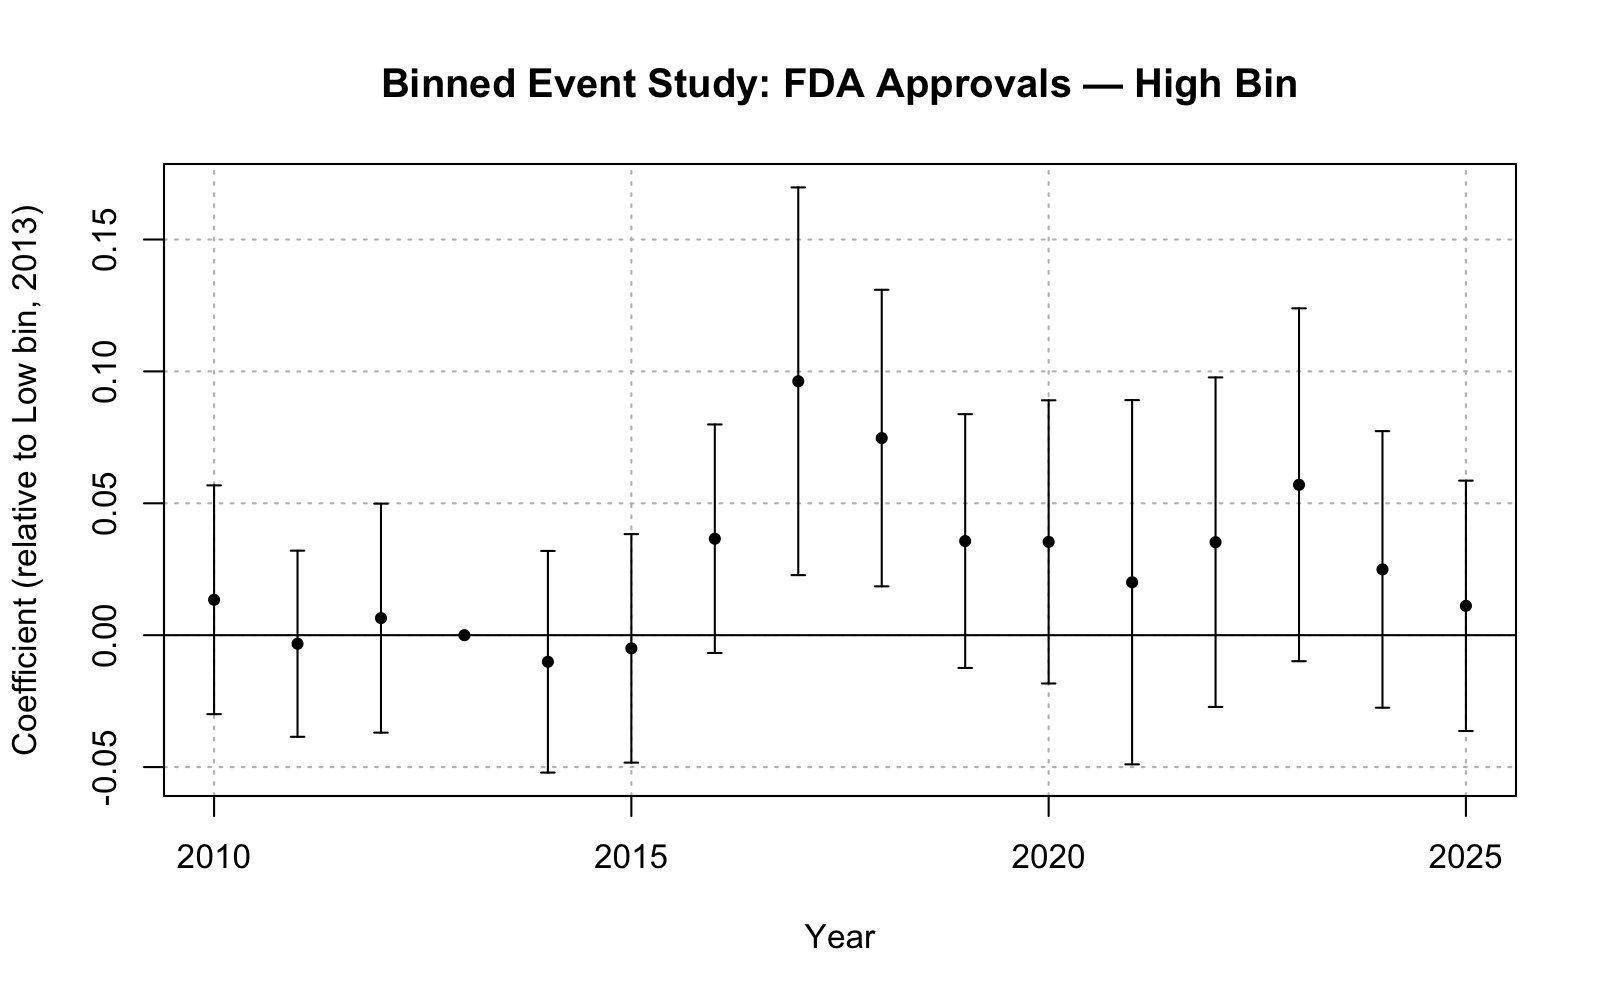
\includegraphics[width=\linewidth]{../output/robustness/binned_treatment/binned_fda_high_es.png}
  \caption{Binned event study: FDA approvals, high-exposure bin (N, C)}
  \label{fig:rob_binned_fda_high}
\end{figure}

\begin{figure}[!h]
  \centering
  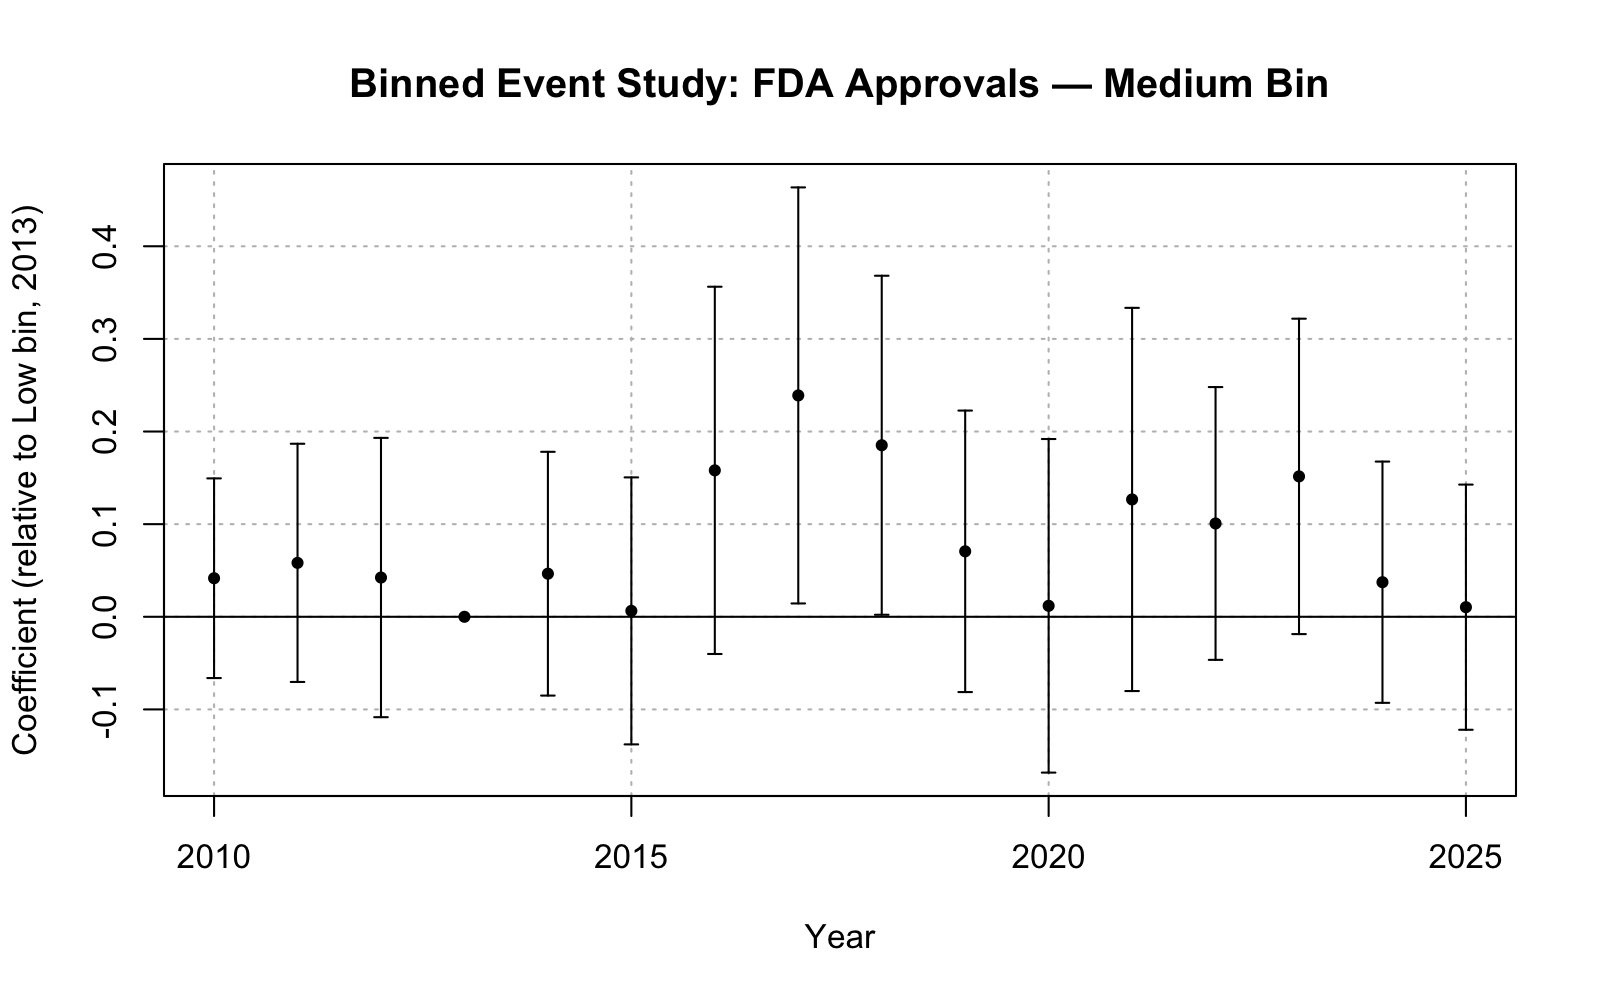
\includegraphics[width=\linewidth]{../output/robustness/binned_treatment/binned_fda_medium_es.png}
  \caption{Binned event study: FDA approvals, medium-exposure bin (J, D)}
  \label{fig:rob_binned_fda_medium}
\end{figure}

\clearpage

\subsubsection{RQ1: Continuous Difference-in-Differences}

%TC:ignore
\makeatletter
\renewenvironment{table}[1][H]{\@float{table}[H]}{\end@float}
\makeatother
\footnotesize
\begin{table}
\centering
\begin{talltblr}[         %% tabularray outer open
entry=none,label=none,
note{}={* 95\% uniform confidence band does not cover 0},
]                     %% tabularray outer close
{                     %% tabularray inner open
colspec={Q[]Q[]Q[]},
column{2,3}={}{halign=c,},
column{1}={}{halign=l,},
hline{8}={1,2,3}{solid, black, 0.05em},
}                     %% tabularray inner close
\toprule
Event Time & Patents & FDA Approvals \\ \midrule %% TinyTableHeader
-3 & \num{0.0038} & \num{-0.0368} \\
   & (\num{0.0034}) & (\num{0.0602}) \\
-2 & \num{0.0023} & \num{0.0361} \\
   & (\num{0.0037}) & (\num{0.0576}) \\
-1 & \num{0.0002} & \num{-0.0326} \\
   & (\num{0.0050}) & (\num{0.0632}) \\
0 & \num{-0.0025} & \num{-0.0506} \\
   & (\num{0.0044}) & (\num{0.0731}) \\
1 & \num{-0.0126} & \num{-0.0092} \\
   & (\num{0.0055}) & (\num{0.0706}) \\
2 & \num{-0.0181}* & \num{0.0646} \\
   & (\num{0.0062}) & (\num{0.0721}) \\
3 & \num{-0.0165} & \num{0.2233} \\
   & (\num{0.0069}) & (\num{0.1018}) \\
4 & \num{-0.0189} & \num{0.1568} \\
   & (\num{0.0073}) & (\num{0.0930}) \\
5 & \num{-0.0271}* & \num{0.0861} \\
   & (\num{0.0080}) & (\num{0.0866}) \\
6 & \num{-0.0313}* & \num{0.1151} \\
   & (\num{0.0082}) & (\num{0.0846}) \\
7 & \num{-0.0315}* & \num{0.0223} \\
   & (\num{0.0084}) & (\num{0.1022}) \\
8 & \num{-0.0333}* & \num{0.0579} \\
   & (\num{0.0083}) & (\num{0.1086}) \\
9 & \num{-0.0348}* & \num{0.1329} \\
   & (\num{0.0084}) & (\num{0.1056}) \\
10 & \num{-0.0358}* & \num{0.0404} \\
   & (\num{0.0085}) & (\num{0.0921}) \\
11 & \num{-0.0324}* & \num{-0.0213} \\
   & (\num{0.0091}) & (\num{0.0919}) \\
\bottomrule
\end{talltblr}
\end{table}

\normalsize
\renewenvironment{table}[1][]{}{}
%TC:endignore

\begin{figure}[!h]
  \centering
  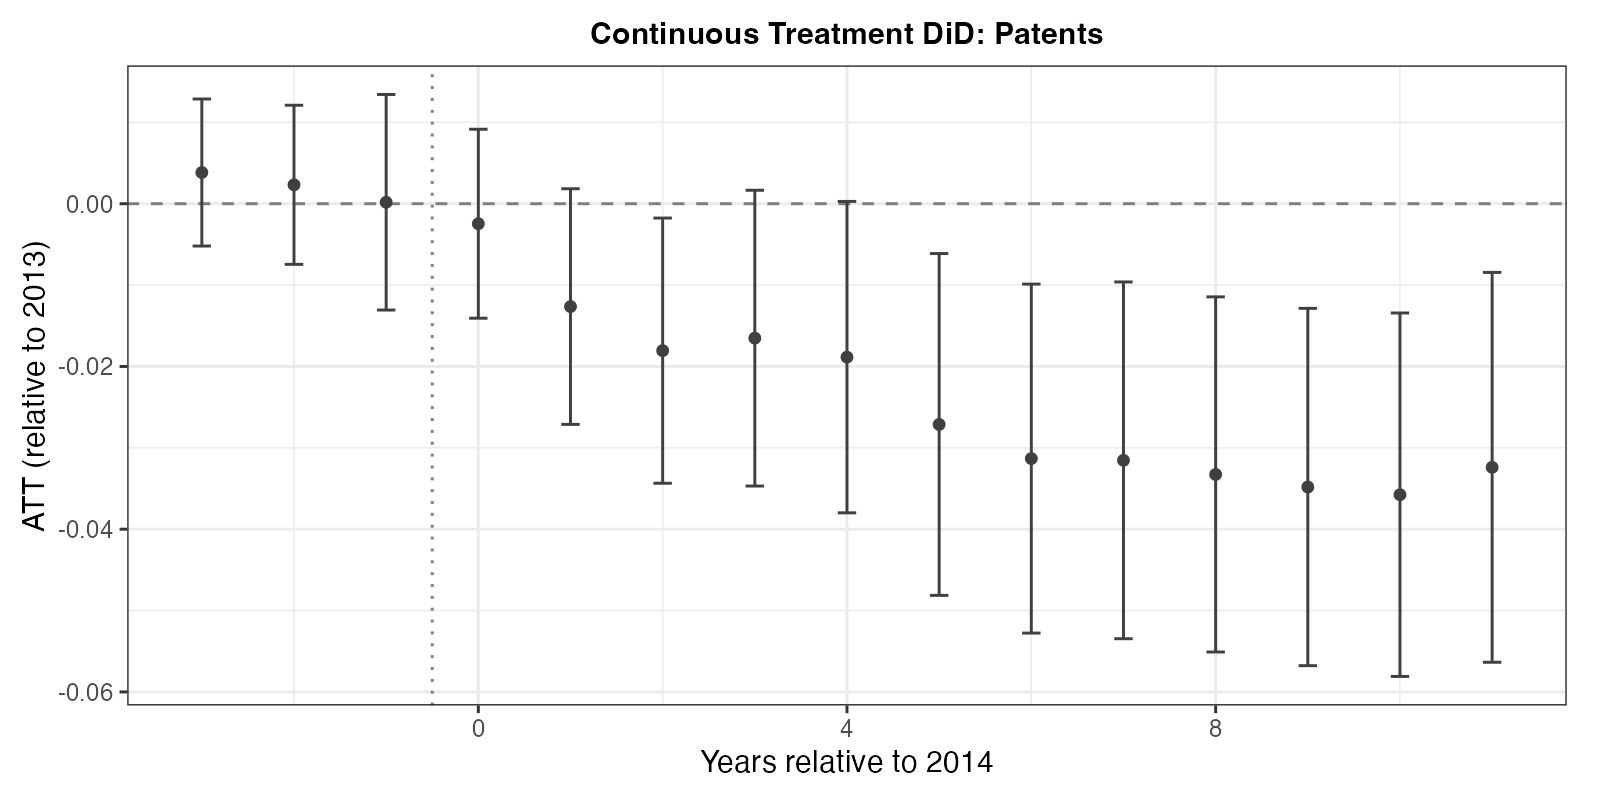
\includegraphics[width=\linewidth]{../output/robustness/contdid/contdid_patent_es.png}
  \caption{Continuous DiD event study: patents}
  \label{fig:rob_contdid_patent}
\end{figure}

\begin{figure}[!h]
  \centering
  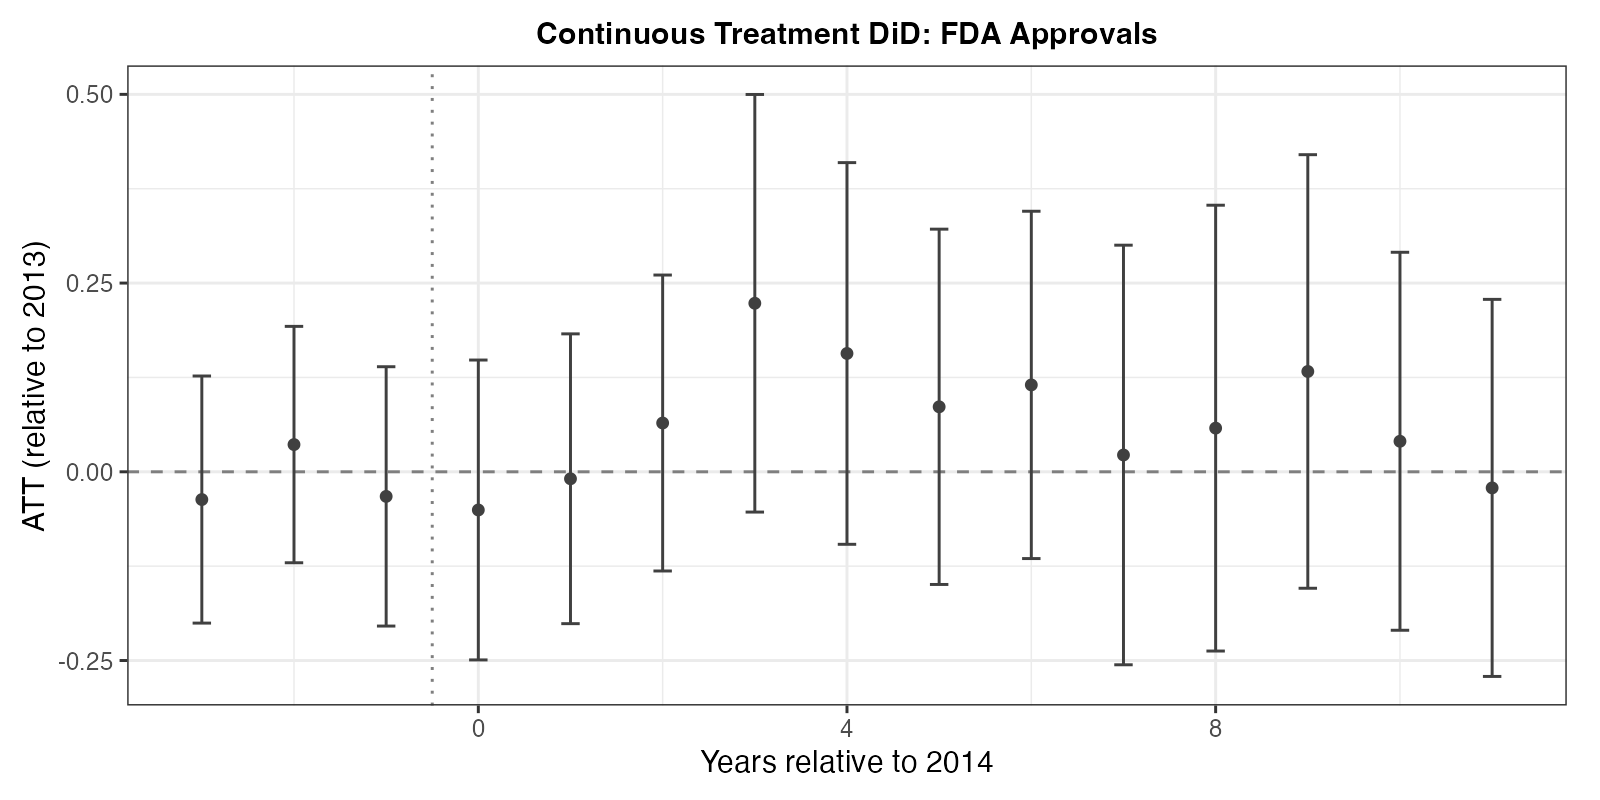
\includegraphics[width=\linewidth]{../output/robustness/contdid/contdid_fda_es.png}
  \caption{Continuous DiD event study: FDA approvals}
  \label{fig:rob_contdid_fda}
\end{figure}

\clearpage

\subsubsection{RQ2: Ex-Post FEOLS}

%TC:ignore
\footnotesize
\begin{table}
\centering
\begin{talltblr}[         %% tabularray outer open
entry=none,label=none,
note{}={* p \num{< 0.05}, ** p \num{< 0.01}, *** p \num{< 0.001}},
]                     %% tabularray outer close
{                     %% tabularray inner open
width=\linewidth,
colspec={Q[]X[]X[]X[]X[]},
column{2,3,4,5}={}{halign=c,},
column{1}={}{halign=l,},
hline{33}={1,2,3,4,5}{solid, black, 0.05em},
}                     %% tabularray inner close
\toprule
& \SetCell[c=2]{c} Patents && \SetCell[c=2]{c} FDA Approvals & \\
& Medicaid Market Share & PDL Exposure & Medicaid Market Share & PDL Exposure \\ \midrule
2010 & \num{-0.033}    & \num{1.546}     & \num{0.285}   & \num{0.046}   \\
     & (\num{0.035})   & (\num{2.018})   & (\num{0.448}) & (\num{0.807}) \\
2011 & \num{-0.010}    & \num{0.734}     & \num{0.344}   & \num{-0.257}  \\
     & (\num{0.033})   & (\num{1.642})   & (\num{0.412}) & (\num{0.711}) \\
2012 & \num{0.005}     & \num{1.079}     & \num{0.371}   & \num{1.395}   \\
     & (\num{0.027})   & (\num{1.289})   & (\num{0.447}) & (\num{0.912}) \\
2014 & \num{-0.017}    & \num{4.161}*    & \num{-0.338}  & \num{0.398}   \\
     & (\num{0.024})   & (\num{1.890})   & (\num{0.536}) & (\num{0.647}) \\
2015 & \num{-0.088}**  & \num{0.836}     & \num{-0.037}  & \num{1.158}   \\
     & (\num{0.027})   & (\num{1.480})   & (\num{0.422}) & (\num{0.881}) \\
2016 & \num{-0.123}*** & \num{-1.554}    & \num{0.456}   & \num{2.642}   \\
     & (\num{0.032})   & (\num{1.620})   & (\num{0.418}) & (\num{1.682}) \\
2017 & \num{-0.123}*** & \num{-1.342}    & \num{1.566}*  & \num{1.924}   \\
     & (\num{0.034})   & (\num{1.890})   & (\num{0.690}) & (\num{0.992}) \\
2018 & \num{-0.136}*** & \num{-2.787}    & \num{1.181}*  & \num{1.683}   \\
     & (\num{0.037})   & (\num{1.644})   & (\num{0.563}) & (\num{1.021}) \\
2019 & \num{-0.195}*** & \num{-3.807}*   & \num{0.359}   & \num{1.171}*  \\
     & (\num{0.039})   & (\num{1.912})   & (\num{0.498}) & (\num{0.591}) \\
2020 & \num{-0.227}*** & \num{-4.650}*   & \num{0.598}   & \num{1.585}   \\
     & (\num{0.041})   & (\num{1.894})   & (\num{0.537}) & (\num{0.942}) \\
2021 & \num{-0.224}*** & \num{-5.267}**  & \num{0.103}   & \num{3.110}*  \\
     & (\num{0.040})   & (\num{1.687})   & (\num{0.583}) & (\num{1.393}) \\
2022 & \num{-0.235}*** & \num{-6.029}**  & \num{0.381}   & \num{0.994}   \\
     & (\num{0.041})   & (\num{1.941})   & (\num{0.593}) & (\num{0.653}) \\
2023 & \num{-0.240}*** & \num{-6.926}*** & \num{0.798}   & \num{1.191}   \\
     & (\num{0.041})   & (\num{1.851})   & (\num{0.583}) & (\num{1.737}) \\
2024 & \num{-0.252}*** & \num{-6.485}*** & \num{0.154}   & \num{-0.447}  \\
     & (\num{0.042})   & (\num{1.788})   & (\num{0.501}) & (\num{0.589}) \\
2025 & \num{-0.212}*** & \num{-4.589}**  & \num{-0.347}  & \num{-1.113}  \\
     & (\num{0.041})   & (\num{1.549})   & (\num{0.525}) & (\num{0.908}) \\
Num. obs. & \SetCell[c=2]{c} \num{5281696} && \SetCell[c=2]{c} \num{151200} & \\
R2        & \SetCell[c=2]{c} \num{0.535}   && \SetCell[c=2]{c} \num{0.609}  & \\
\bottomrule
\end{talltblr}
\end{table}

\captionof{table}{FEOLS event-study estimates: Medicaid demand and PDL exposure (ex-post)}
\label{tab:rob_rq2_feols_expost}
\normalsize
%TC:endignore

\begin{figure}[!h]
  \centering
  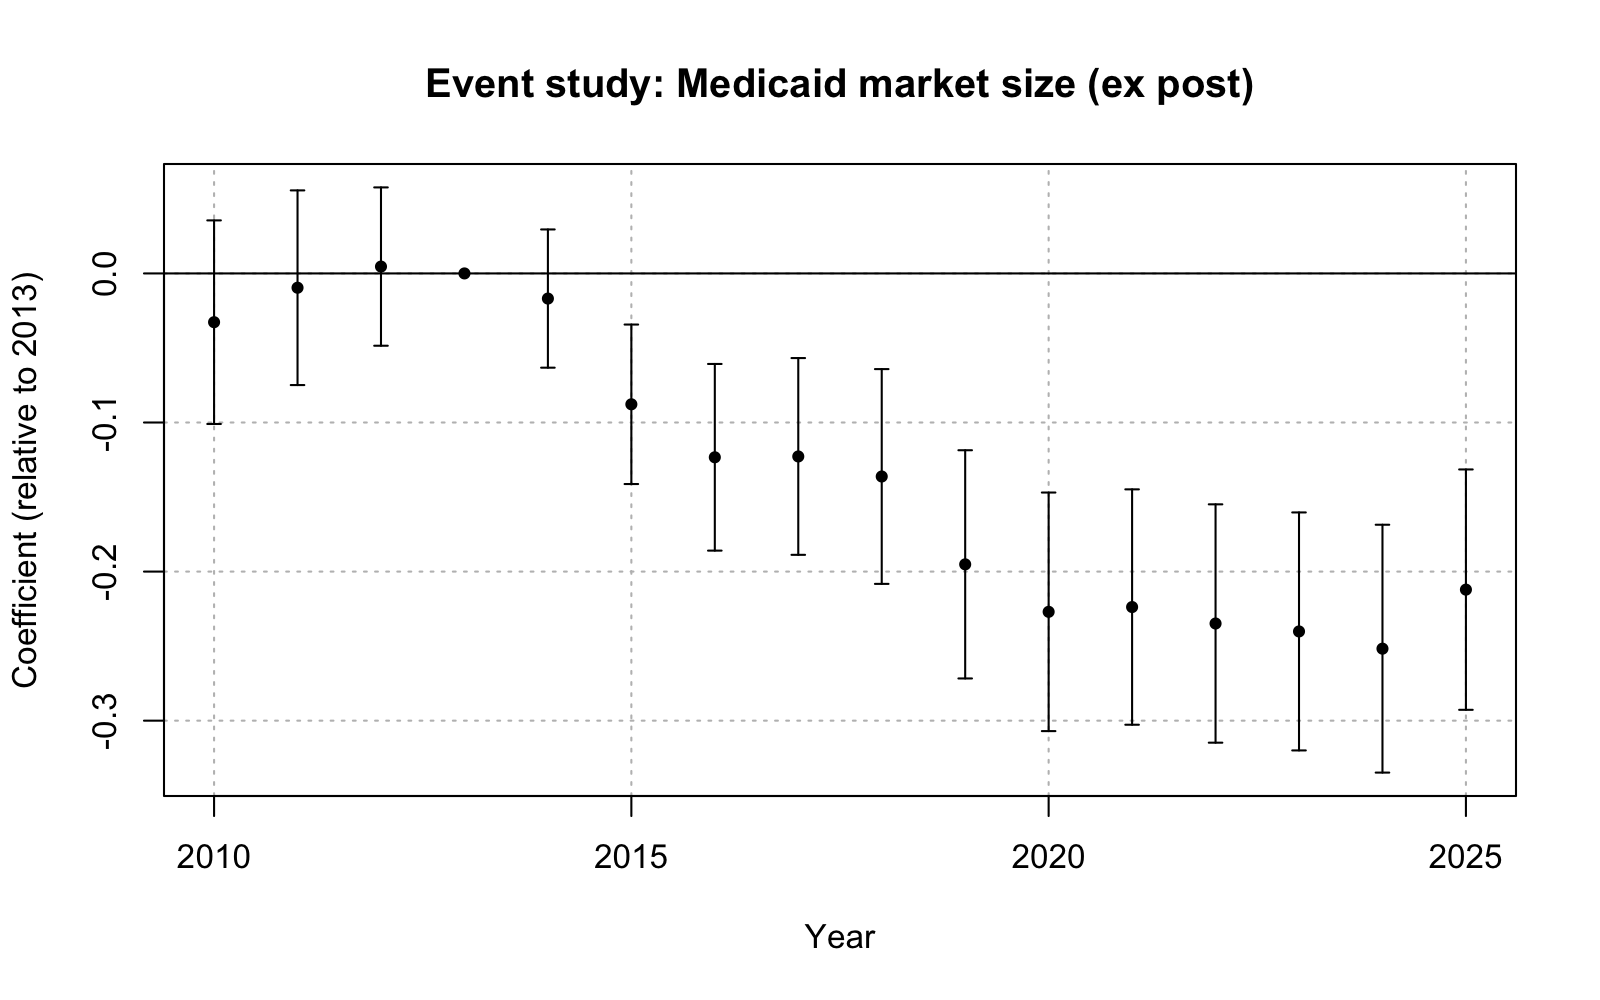
\includegraphics[width=\linewidth]{../output/RQ2/patent_feols_expost_medicaid.png}
  \caption{FEOLS event study: patents, Medicaid exposure (ex-post)}
  \label{fig:rob_rq2_patent_expost_medicaid}
\end{figure}

\begin{figure}[!h]
  \centering
  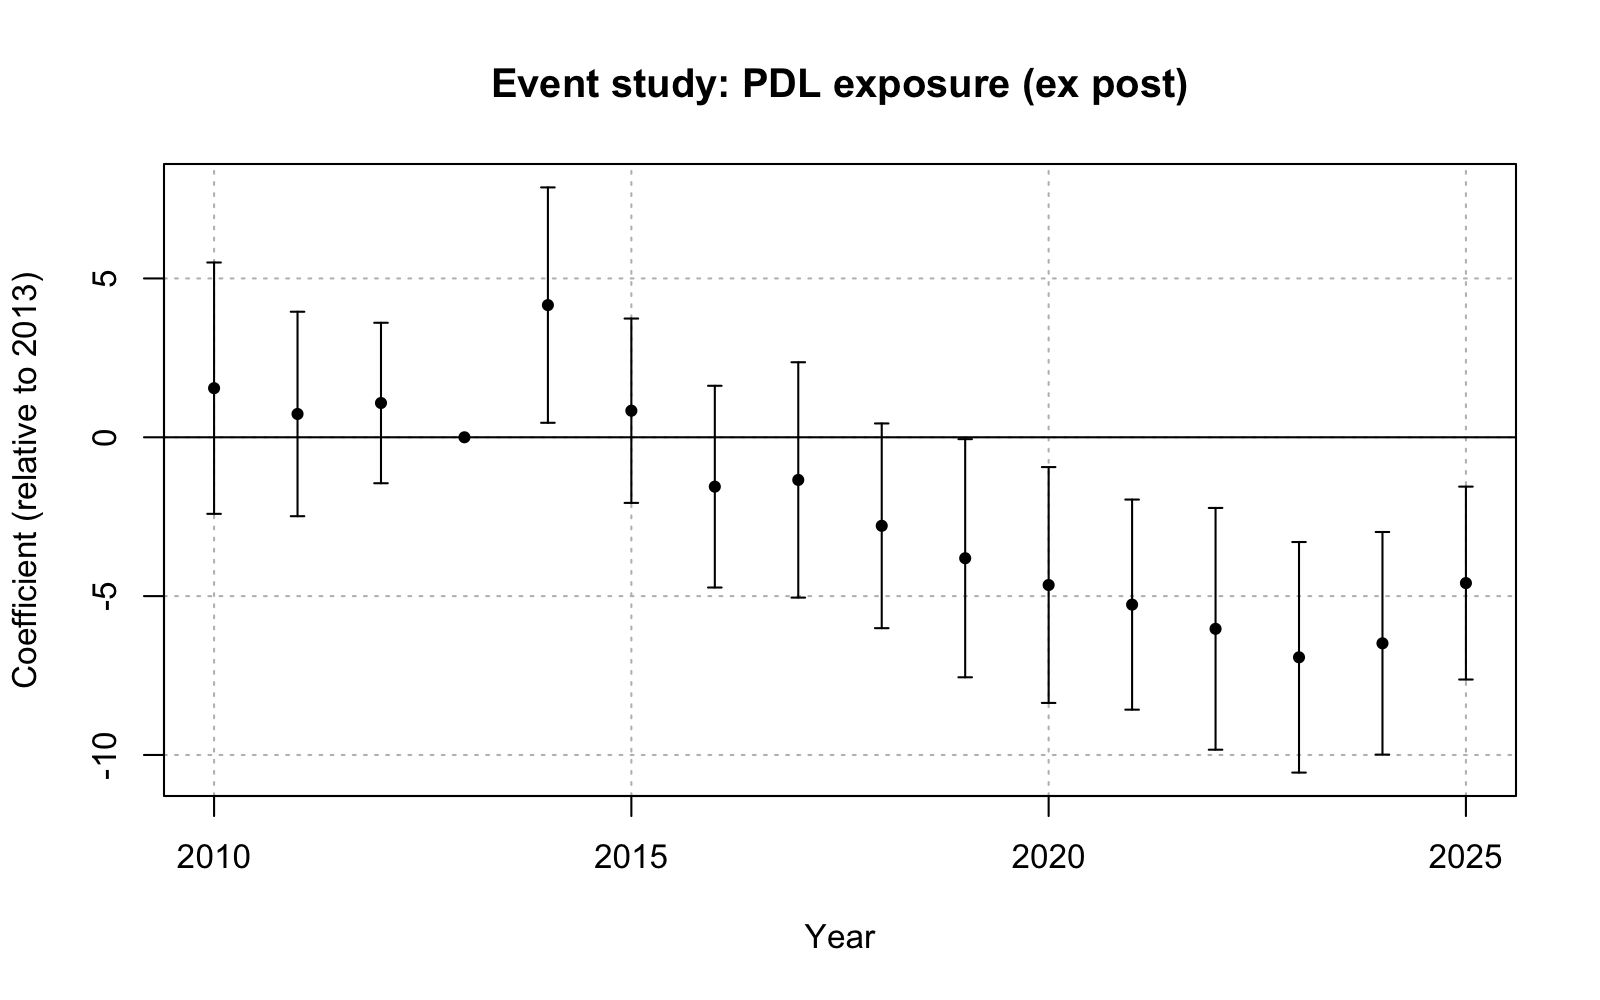
\includegraphics[width=\linewidth]{../output/RQ2/patent_feols_expost_pdl.png}
  \caption{FEOLS event study: patents, PDL exposure (ex-post)}
  \label{fig:rob_rq2_patent_expost_pdl}
\end{figure}

\clearpage

\begin{figure}[!h]
  \centering
  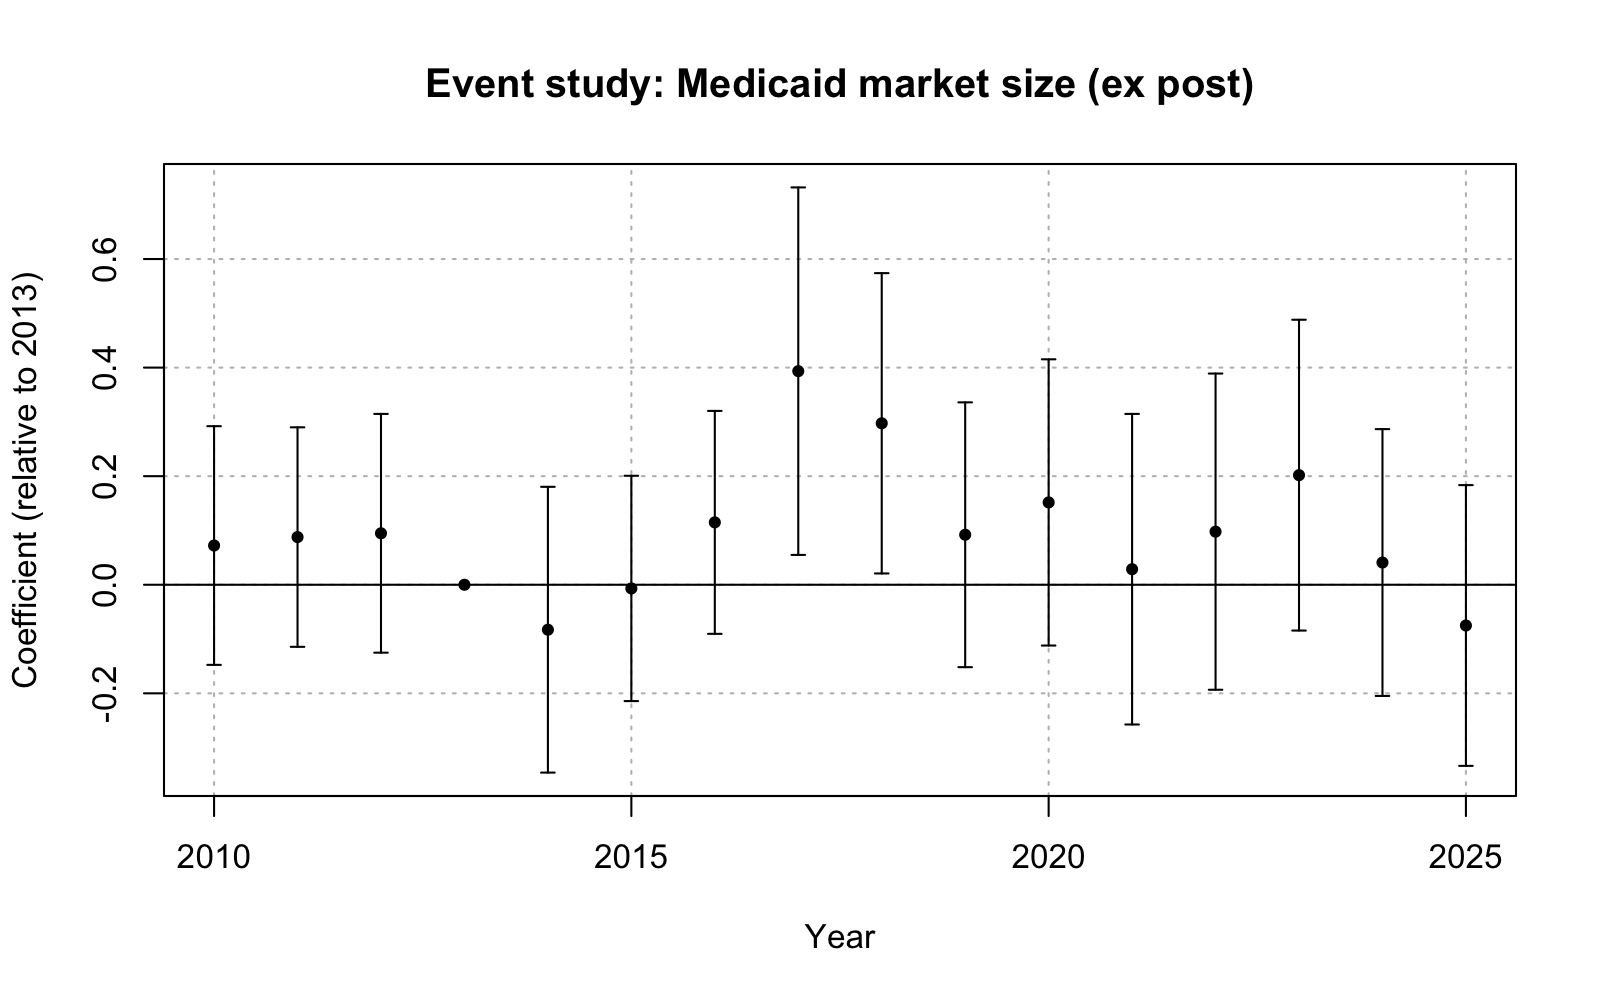
\includegraphics[width=\linewidth]{../output/RQ2/fda_feols_expost_medicaid.png}
  \caption{FEOLS event study: FDA approvals, Medicaid exposure (ex-post)}
  \label{fig:rob_rq2_fda_expost_medicaid}
\end{figure}

\begin{figure}[!h]
  \centering
  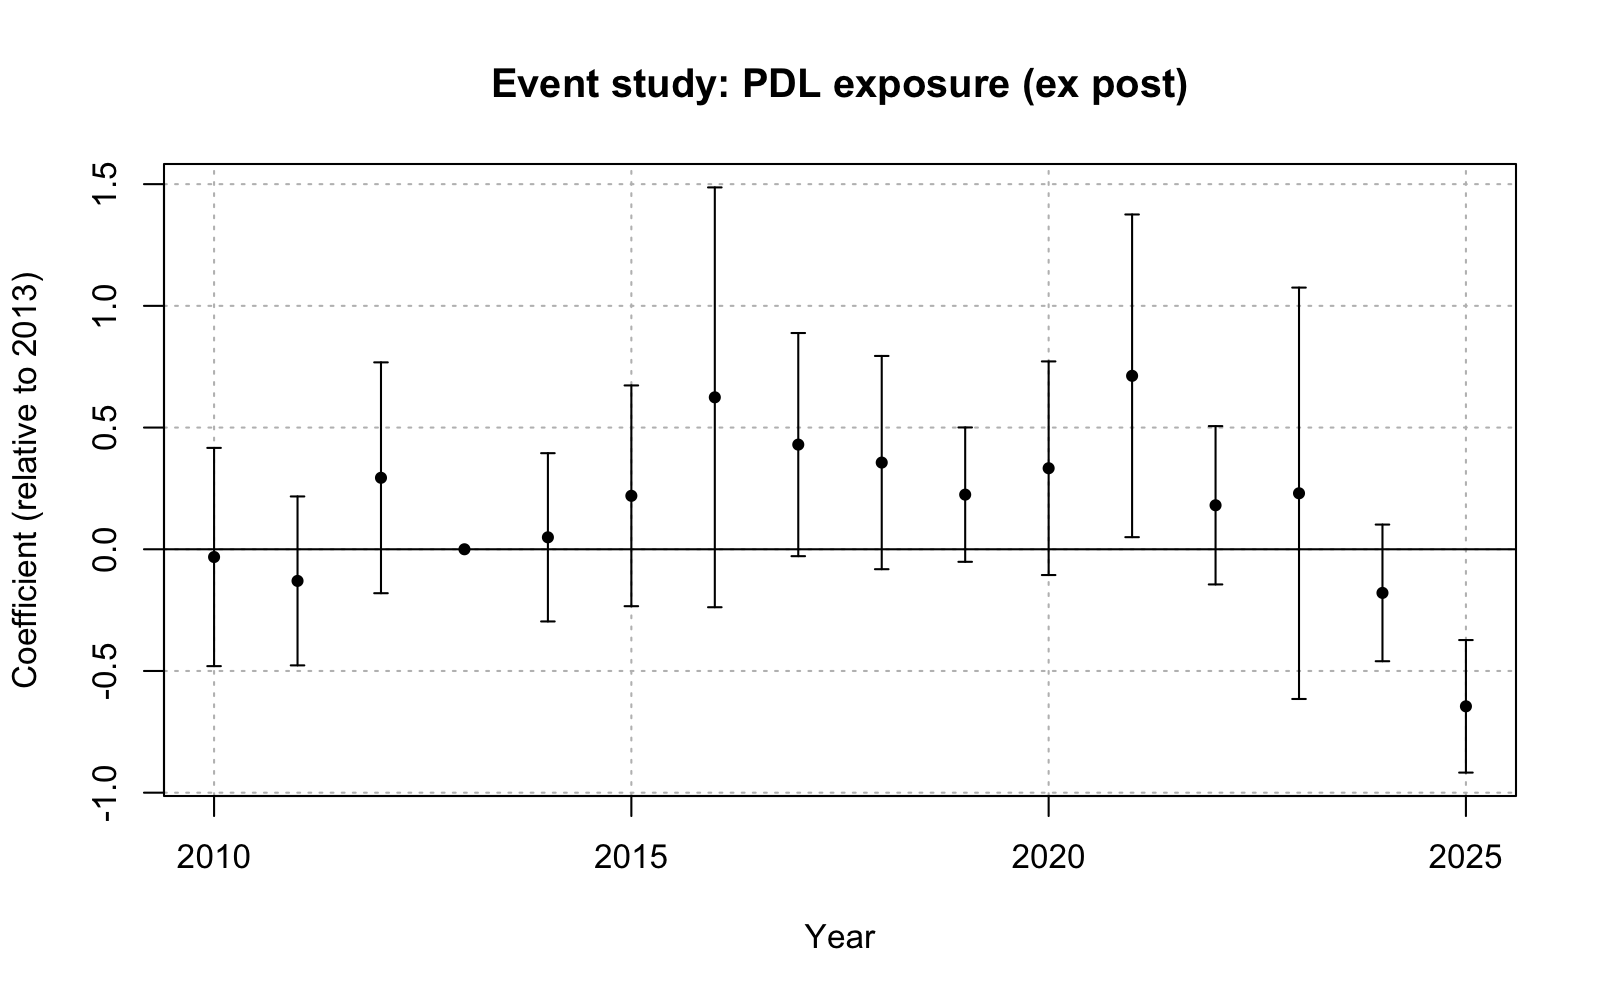
\includegraphics[width=\linewidth]{../output/RQ2/fda_feols_expost_pdl.png}
  \caption{FEOLS event study: FDA approvals, PDL exposure (ex-post)}
  \label{fig:rob_rq2_fda_expost_pdl}
\end{figure}

\clearpage

\subsubsection{RQ3: Ex-Post FEOLS}

%TC:ignore
\footnotesize
\begin{table}
\centering
\begin{talltblr}[         %% tabularray outer open
entry=none,label=none,
note{}={* p \num{< 0.05}, ** p \num{< 0.01}, *** p \num{< 0.001}},
]                     %% tabularray outer close
{                     %% tabularray inner open
colspec={Q[]Q[]Q[]},
column{2,3}={}{halign=c,},
column{1}={}{halign=l,},
hline{26}={1,2,3}{solid, black, 0.05em},
}                     %% tabularray inner close
\toprule
& Patents & FDA Approvals \\ \midrule
Medicaid Share × ATC = A & \num{-0.157}*** & \num{1.301}**  \\
& (\num{0.031})   & (\num{0.420})  \\
Medicaid Share × ATC = B & \num{0.151}***  & \num{-0.121}   \\
& (\num{0.027})   & (\num{0.784})  \\
Medicaid Share × ATC = C & \num{-0.094}*** & \num{0.373}    \\
& (\num{0.015})   & (\num{0.278})  \\
Medicaid Share × ATC = D & \num{-0.017}    & \num{0.881}**  \\
& (\num{0.062})   & (\num{0.337})  \\
Medicaid Share × ATC = G & \num{0.032}     & \num{-1.058}   \\
& (\num{0.049})   & (\num{1.121})  \\
Medicaid Share × ATC = H & \num{0.619}***  & \num{0.446}    \\
& (\num{0.096})   & (\num{0.530})  \\
Medicaid Share × ATC = J & \num{0.035}     & \num{-0.078}   \\
& (\num{0.034})   & (\num{0.089})  \\
Medicaid Share × ATC = L & \num{0.443}     & \num{-0.244}   \\
& (\num{0.578})   & (\num{2.115})  \\
Medicaid Share × ATC = M & \num{-0.212}*** & \num{0.017}    \\
& (\num{0.048})   & (\num{0.858})  \\
Medicaid Share × ATC = N & \num{-0.174}*** & \num{0.047}    \\
& (\num{0.039})   & (\num{0.101})  \\
Medicaid Share × ATC = R & \num{0.005}     & \num{0.178}    \\
& (\num{0.003})   & (\num{0.130})  \\
Medicaid Share × ATC = S & \num{0.105}***  & \num{6.473}*   \\
& (\num{0.020})   & (\num{3.004})  \\
Num. obs.                & \num{19617728}  & \num{561600}   \\
R2                       & \num{0.247}     & \num{0.235}    \\
\bottomrule
\end{talltblr}
\end{table}

\captionof{table}{Triple-difference estimates: therapeutic-class heterogeneity (FEOLS, ex-post)}
\label{tab:rob_rq3_feols_expost}
\normalsize
%TC:endignore

\clearpage

% --- From theoretical_model.tex ---

\subsection{Baseline Model Parameters} \label{app:parameters}

Table~\ref{tab:parameters} reports the baseline parameter values used to generate Figure~\ref{fig:comp_statics}. Parameters that are not varied are held at these baseline values.

%TC:ignore
\makeatletter
\renewenvironment{table}[1][H]{\@float{table}[H]}{\end@float}
\makeatother
\begin{table}[H]
\centering
\caption{Baseline parameter values used for comparative statics simulations}
\label{tab:parameters}
\begin{tblr}{
    width = \textwidth,
    colspec = {X[c,0.8] X[l,3.4] X[c,1.2]},
    row{1} = {halign=c}
}
\toprule
Parameter & Description & Baseline Value \\
\midrule
$\sigma$      & Std.\ dev.\ of the innovation shock $\varepsilon_i$                   & $1.0$           \\
$\bar{a}$     & Clinical quality threshold (P\&T approval bar)                        & $0.5$           \\
$\bar{p}$     & Regulatory price cap                                                  & $10.0$          \\
$\bar{c}$     & Expected marginal cost                                                & $2.0$           \\
$k$           & Effort cost scaling parameter                                         & $1.0$           \\
$\alpha_c$    & Rebate scale parameter                                                & $0.02$          \\
$\beta_c$     & Rebate elasticity under power form $\tau_c = \alpha_c M_c^{\beta_c}$ & $0.75$          \\
$c$           & Marginal cost distribution in the duopoly auction                     & $U[0.5,\, 3.5]$ \\
$M_0$         & Reference market size                                                 & $100$           \\
$\delta$      & Period 2 cost reduction factor                                        & $0.7$           \\
\bottomrule
\end{tblr}
\end{table}
\renewenvironment{table}[1][]{}{}
%TC:endignore

\end{document}
%
}

\begin{document}

% ===== Title Page =====
\begin{titlepage}
  \centering
  \vspace*{3cm}
  {\LARGE\bfseries MPhil Thesis\par}
  \vspace{1.5cm}
  {\Large Mohammad-Shah Karim\par}
  \vspace{1cm}
  {\large May 2026\par}
  \vspace{2cm}
  {\large Word count: \totalwordcount\par}
  \vfill
\end{titlepage}

% ===== Table of Contents =====
\mastertoc
\newpage

% ===== Main Body =====
\documentclass[12pt]{article}
\usepackage{geometry}
\geometry{a4paper, portrait, margin=1in}

% --- Math Packages ---
\usepackage{amsmath}
\usepackage{amssymb}
\usepackage{amsfonts}
\usepackage{amsthm}

% --- Graphics & Diagrams ---
\usepackage{graphicx}
\usepackage{tikz}
\usetikzlibrary{shapes, arrows, positioning}

% --- Formatting ---
\usepackage{parskip}
\usepackage[hidelinks]{hyperref}
\usepackage{natbib}
\usepackage{enumitem}
\pagestyle{plain}

\title{MPhil Thesis: Introduction}
\author{Mohammad-Shah Karim}
\date{April 2026}

\begin{document}

\maketitle

\section{Introduction}

Pharmaceutical innovation is central towards long-run improvements in health and welfare. New drugs can improve quantity of life while changing the treatment possibilities which are available for physicians to administer on patients. At the same time, pharmaceutical innovation is unusually sensitive to policy. Development of a new drug requires a large upfront investment with a long development horizon including patent applications and clinical trials, with only a high probability of failure. Since the returns to a successful drug accrue over multiple years and depend on both prices and the volumes that prevail within the market, the incentives to undertake the investment to develop a drug are shaped not only by opportunity, but also by the economic and institutional environment present which determine the expected future profits once the drug reaches the market.

This makes the pharmaceutical market within the United States of America an ideal setting for studying how public policy shapes scientific opportunity. Federal and state governments are now responsible for roughly half of all prescription drug spending (INSERT SOURCE HERE), both as direct purchasers through programmes such as Medicaid and Medicare, and also indirectly through the tax preferences and regulatory rules that govern private insurance. Medicaid is especially important in this respect - it is a large public buyer, but it does not operate as a standard private insurer. Manufacturers that wish to have Medicaid coverage must participate in the Medicaid Drug rebate Program, and states can use Preferred Drug Lists (PDLs) in order to negotiate additional rebates in exchange for preferred formulary placement. Given this, Medicaid demand passes through a public procurement system with statutory and supplement rebates in addition to state level formulary bargaining, thus it cannot be treated as additional market demand.

This thesis examines the consequences of one of such reforms for pharmaceutical innovation - the 2014 Medicaid expansion under the the Patient Protection and Affordable Care Act (ACA). The reform produced a well-documented expansion in the size of the Medicaid market, with population coverage increasing by close to twenty million enrollees int he years following the policy change (INSERT SOURCE HERE). Under standard market-sized frameworks in the pharmaceutical sector this should increase innovation incentives for drug-classes more exposed to Medicaid demand \citep{finkelstein2004static, dubois2015market}. If firms expect to sell more units after a successful round of innovation, the expected returns to R\&D rise. However, the expansion of Medicaid took place inside a procurement framework that combined two features of that are unusual under the standards of a private insurer. A statutory rebate schedule that mechanically transfers a share of any list-price revenue back to the state, and a state-administered formulary system in which Preferred Drug Lists (PDLs) determine which products are reimbursed without prior authorisation. Thus the institutional features meant that an expansion of Medicaid was not simply a positive demand shock for pharmaceutical firm.

The Medicaid setting therefore complicates the prediction under standard pharmaceutical market-sized frameworks. The ACA did not only expand the number of beneficiaries under Medicaid, but it also raised the statutory rebate percentages and extended rebate obligations to Medicaid managed care. Therefore, the reform increased the size of the public market while also increasing the share of revenue back to the state. Additionally, as Medicaid demand grows, preferred placement on a state PDL becomes more valuable. States can use this to negotiate deeper rebates from manufacturers. The same policy may therefore generate two opposing effects. On the one hand, Medicaid expansion raises demand. On the other hand, it may increase pricing pressure and reduce the surplus that firms can capture from that demand.

This thesis therefore raises the question of whether the ACA-induced Medicaid expansion raised pharmaceutical innovation, and whether the response dependent on a firm's exposure to the Medicaid procurement institutions. Put simply, was the expected positive relationship between market size and innovation weakened when the additional demand flows through a state-wide monopsony. Many current drug-pricing reforms, including recent Medicare negotiation policies, rely on the same basic trade-off: lowering public spending and consumer prices may increase static welfare, but it may also affect the expected returns to future innovation, raising the relevance of this question


\newpage
\bibliographystyle{apalike}
\bibliography{references}

\end{document}

\documentclass[12pt]{article}
\usepackage{geometry}
\geometry{a4paper, portrait, margin=1in}

% --- Math Packages ---
\usepackage{amsmath}
\usepackage{amssymb}
\usepackage{amsfonts}
\usepackage{amsthm}

% --- Graphics & Diagrams ---
\usepackage{graphicx}
\usepackage{tikz}
\usetikzlibrary{shapes, arrows, positioning}

% --- Formatting ---
\usepackage{parskip}
\usepackage[hidelinks]{hyperref}
\usepackage{natbib}
\usepackage{enumitem}
\usepackage{booktabs}
\usepackage{caption}
\usepackage{siunitx}
\usepackage{tabularray}
\UseTblrLibrary{booktabs, siunitx}
\pagestyle{plain}

% --- Word count (requires compiling with --shell-escape) ---
\newcommand{\wordcount}{%
  \immediate\write18{texcount -sum -1 \jobname.tex 2>/dev/null | python3 -c "import sys; n=sys.stdin.read().strip(); print(f'{int(n):,}') if n.isdigit() else print('?')" > \jobname.wc}%
  \input{\jobname.wc}%
}

\title{MPhil Thesis: Literature Review}
\author{Mohammad-Shah Karim}
\date{May 2026}

\begin{document}

\maketitle

\begin{center}
  \small Word count: \wordcount
\end{center}

\tableofcontents

\newpage

\section{Literature Review}

This thesis sits at the intersection of the literature on pharmaceutical innovation and how the institutional settings behind public reimbursement shape firm incentives. It also draws on work examining the timing of innovation measures across the drug-development pipeline

Before turning to these areas, it is beneficial to understand the current studies on the ACA Medicaid expansion. The reform yielded large gains in concentrated in states that chose to expand access to Medicaid, with the gaps in racial and ethnic coverage narrowing as a result \citep{courtemanche2020impact, frean2017premium, miller2019four}. These states saw increased affordability indicating reductions in the cost barriers for accessing healthcare \citep{miller2017health}, alongside declines in medical debt and bankruptcy from healthcare \citep{brevoort2017medicaid, HU201899}. These increases in access and financial welfare were accompanies with improvements in self-reported health and reductions in adult mortality \citep{miller2021medicaid, miller2017health}. However, evidence on labour market effects has been more limited, where no no significant changes were recorded in employment outcomes or physician hours \citep{duggan2019effects, dague2017effect, neprash2021effect}. This thesis studies a less explored dimension of the Medicaid expansion - its effects on pharmaceutical innovation.

\subsection{Market Size and Pharmaceutical Innovation}



\subsection{Medicaid Expansion and Pharmaceutical Innovation}

The most closely related study to this thesis is \cite{NBERw28755}, which examines the impact of the ACA Medicaid expansion on clinical trial activity. With the use of disease condition Medicaid market shares as a proxy for Medicaid exposure, they find no evidence of a significant innovation response through to 2016. They propose that this null result may reflect the lower expected returns associated with Medicaid relative to reforms such as Medicare Part D, due to manufacturer revenue being constrained by the rebates and price controls embedded within the programme.

While this finding is an important starting point to address the question, their analysis leaves several gaps which this thesis addresses. First, the post-expansion window is constrained by both the innovation outcome studied and the length of the post-expansion window. \citeauthor{NBERw28755} investigated clinical trial activity through to 2016, so their estimates only capture the first two years of the Medicaid demand shock. This is short relative to the development horizon for pharmaceutical drug development, which can span between five to twenty years \citep{brown2022clinical}. As a result, the absence of a response in clinical trials cannot distinguish between an innovation effect that is genuinely absent, or one that has affected early stage R\&D decisions but has not reached the clinical trials stage.

Second, the absence of an aggregate clinical-trial response does not confirm whether the innovation effect differs across therapeutic classes. \citet{sutton1998technology} argues that pharmaceutical R\&D is organised around narrow chemically related drug groups rather than broad therapeutic categories, and finds limited persistence in firms' major follow-on successes within these groups. This suggests that therapeutic-class-level aggregates may conceal meaningful heterogeneity in how firms adjust innovation activity. Instead, an insignificant aggregate relationship may be driven by heterogeneous responses across drug classes. Positive R\&D responses may have occurred in classes where the market-size channel dominated, but the aggregate effect may have been offset by negative clinical-trial responses in areas where the expansion weakened innovation incentives.

Third, while \citeauthor{NBERw28755} propose that the lower returns to the Medicaid market may explain the contrast with earlier market-size studies that find positive innovation responses, this explanation lies outside of their empirical design. Specifically, their analysis does not control for the procurement institutions that may affect manufacturer profits, including rebate pressures and formulary placement on Medicaid's PDL.

This thesis addresses these gaps by extending the analysis across the innovation pipeline, across time, and across therapeutic markets. First, this thesis constructs novel panels linking firms to their drugs in Medicaid's State Drug Utilisation Data, and then to their patenting and FDA approval activity. These innovation outcomes bracket the clinical-trial stage examined by \citeauthor{NBERw28755}, allowing earlier and later innovation responses to be considered separately. Second, the impact of the reform is investigated over a substantially longer post-expansion period, with outcome data extending to 2025, whereas \citeauthor{NBERw28755} used data ending in 2016. This extension allows delayed innovation responses to be captured more clearly, which is particularly important given the long development horizon in pharmaceutical R\&D. Third, class-level heterogeneous responses are examined to determine whether the expansion generated different innovation incentives across the therapeutic markets in which firms operated in, rather than restricting the analysis to an average therapeutic-area effect.

\citeauthor{NBERw28755} cite the Medicaid procurement mechanism as a potential reason for the inconclusive results, thus this thesis addresses this paper directly in the empirical analysis with the use of firm-class exposure to Medicaid's PDL. This is complemented by a counterfactual analysis of the clinical and pricing stages of preferred placement on the PDL, alongside a theoretical model in which market expansion interacts with rebates and placement on Medicaid's formulary to shape innovation incentives.

\subsection{Medicaid Pricing and Manufacturer Incentives}

Medicaid prescriptions are subject to statutory rebates under the MDRP, and each state can negotiate supplemental rebates with manufacturers in exchange for preferred placement on the PDL. \cite{duggan2006distortionary} show that these rules create incentives for manufacturers to raise prices for non-Medicaid consumers, since drug prices and reimbursement offered to Medicaid is linked to the prices charged in the private market. Consequently, the results highlight that manufacturers segment drug demand separately for the Medicaid and private markets, amd the ACA may have intensified this distortion by raising the statutory rebate from 15.1\% to 23.1\% of AMP. \cite{feng2023profiting} find that the higher statutory rebates relaxed the constraints imposed by Medicaid's most favoured customer clause allowing private customers to benefit with lower prices and lower drug spending by 2.5\%. Together, these findings show that Medicaid's rebate rules have spillover effects on pricing incentives outside of Medicaid, but the direction of the effect depends on the institutional channel through which the rebate structure operates.

Related structural work shows that pharmaceutical pricing rules can alter manufacturers' pricing behaviour to offset reductions in per prescription revenues. \cite{dubois2022bargaining} show that firms adjust pricing and bargaining behaviour when price regulations in one market can impact profits elsewhere, indicating that the effect of pricing institutions on manufacturer returns depend on how firms respond strategically across markets.

However, \cite{inderst2007buyer} show that larger buyers can raise incentives for incremental forms of product innovation, while weakening incentives for more substantial novel R\&D. This distinction is crucial in the Medicaid setting, where the expansion increases market size, while also raising exposure to the formulary selection, which may weaken incentives for more inventive forms of innovation. Therefore, this is addressed empirically in the Medicaid setting by studying patent applications, which capture early stage R\&D behaviour undertaken in anticipation of future returns. FDA approvals are used to assess whether any upstream innovation response is eventually reflected in regulatory outcomes.

\subsection{Innovation Pipeline Timing}


\clearpage

\bibliographystyle{apalike}
\bibliography{references}

\end{document}
\documentclass[12pt]{article}
\usepackage{geometry}
\geometry{a4paper, portrait, margin=1in}

% --- Math Packages ---
\usepackage{amsmath}
\usepackage{amssymb}
\usepackage{amsfonts}
\usepackage{amsthm}

% --- Graphics & Diagrams ---
\usepackage{graphicx}
\usepackage{tikz}
\usetikzlibrary{shapes, arrows, positioning}

% --- Formatting ---
\usepackage{parskip}
\usepackage[hidelinks]{hyperref}
\usepackage{natbib}
\usepackage{enumitem}
\usepackage{booktabs}
\pagestyle{plain}

\title{MPhil Thesis: Data}
\author{Mohammad-Shah Karim}
\date{April 2026}

\begin{document}

\maketitle

\tableofcontents

\newpage

\section{Data}

\subsection{Overview and Unit of Observation}

The empirical analysis draws on five sources: the Medicaid State Drug Utilisation Data (SDUD) maintained by the Centers for Medicare and Medicaid Services (CMS); the Drugs@FDA database; patent bulk data files distributed by the USPTO through the PatentsView project; the Texas Vendor Drug Program formulary; and the National Library of Medicine's RxNorm and RxClass systems, which provide the therapeutic classification bridge across sources. Table~\ref{tab:data_overview} summarises the contribution of each source to the final dataset.

\begin{table}[htbp]
\centering
\caption{Data sources and their roles in the analysis}
\label{tab:data_overview}
\begin{tabular}{p{0.25\textwidth} p{0.25\textwidth} p{0.40\textwidth}}
\toprule
Source & Key identifier & Role \\
\midrule
SDUD (CMS) & NDC, state, year, quarter & Medicaid and non-Medicaid prescription volumes and reimbursement \\
Drugs@FDA & Application number, sponsor name & FDA drug approval outcomes \\
USPTO / PatentsView & Patent ID, assignee name & Patent counts by therapeutic class \\
Texas Vendor Drug Program & NDC, effective date & PDL status and prior authorisation indicators \\
RxNorm / RxClass & RxCUI, ATC code & Therapeutic classification of NDC and active ingredients \\
\bottomrule
\end{tabular}
\end{table}

The final estimation dataset is a balanced panel at the firm $\times$ ATC Level 1 $\times$ year $\times$ quarter level, spanning 2010 to 2025. The sample period begins in 2010 because the pre-expansion Medicaid exposure measures require at least two years of pre-reform prescription data, and the SDUD is downloaded from 2005 onwards for this purpose. All datasets are harmonised to the World Health Organisation's Anatomical Therapeutic Chemical (ATC) classification system at Level 1, as described in Section~\ref{sec:atc}. The construction of treatment and outcome variables, including the Medicaid exposure measures and PDL exposure variables, is described in the Methodology section.

\subsection{Medicaid State Drug Utilisation Data}
\label{sec:sdud}

The main source for Medicaid prescription demand is the State Drug Utilisation Data (SDUD), maintained by the Centers for Medicare and Medicaid Services (CMS). The SDUD was established alongside the Medicaid Drug Rebate Program and records outpatient prescription drugs reimbursed by state Medicaid programmes at the drug $\times$ state $\times$ quarter level. It covers all fifty states and the District of Columbia. Each record is identified by an 11-digit National Drug Code (NDC) and reports prescription counts, units reimbursed, and reimbursement amounts split into Medicaid and non-Medicaid components. Annual files covering 2005 to 2024 are downloaded via the Medicaid Data portal API, yielding a raw dataset of 42,031,131 records.

The SDUD plays two roles in the analysis. First, it is used to construct Medicaid exposure measures at the therapeutic-class - this forms the main treatment variable for the analysis. Secondly, once merged with PDL information from the Texas Vendor Drug Program, the SDUD is used to construct exposure measures to formulary placement and pricing pressure at the firm-level.

\begin{table}[htbp]
\centering
\caption{Key variables in the SDUD}
\begin{tabular}{p{0.28\textwidth} p{0.62\textwidth}}
\toprule
Variable & Description \\
\midrule
NDC & 11-digit code identifying each drug product, split into a 5-digit labeler code, 4-digit product code, and 2-digit package code \\
Drug name & Proprietary or generic name of the drug \\
Units reimbursed & Number of units reimbursed by Medicaid in the state-year-quarter cell \\
Number of prescriptions & Number of prescriptions filled for a given drug in the state-year-quarter cell \\
Reimbursement amount & Total reimbursement for a given drug, split into Medicaid and non-Medicaid components \\
\bottomrule
\end{tabular}
\end{table}

\subsubsection{National Drug Code structure}

The NDC is an 11-digit product identifier - this contains a 5-digit labeler code, a 4-digit product code, and a 2-digit package code. The SDUD stores the NDC as an 11-digit string without hyphens. However, throughout this analysis the labeler, product, and package components are extracted by splitting on character position (positions 1-5, 6-9, 10-11). External sources that use the hyphenated three-segment format such as the FDA NDC directory require the inverse transformation where each raw segment is zero-padded to its standard width before concatenation. This normalisation is applied uniformly across all datasets to ensure that NDC-based joins do not introduce incorrect matches due to formatting differences.

\subsubsection{Firm identification}

The SDUD does not record firm names, so firms are instead identified through their NDC labeler code. However, pharmaceutical firms commonly operate with the use of multiple labeler codes due to  subsidiaries or acquisition arrangements. As a result, labeler codes alone cannot be treated as a unique firm identifier in this analysis.

A firm mapping is constructed from the FDA NDC directory. Each labeler code is initially linked to its registered labeler name from the FDA's product and package text files. These names are then clustered into firm-level groups using a text similarity procedure. Labeler names are standardised by converting to lowercase, removing punctuation, and stripping trailing whitespace. Unigram tokenisation is then used to construct a term frequency-inverse document frequency (TF-IDF) representation, and pairwise cosine similarity is computed across all cleaned labeler names. Pairs with a cosine similarity score above 0.85 are treated as matches and are grouped into firm clusters, so that labeler codes with sufficiently similar names are assigned to the same firm. Each cluster is assigned the name of its first member as the canonical firm identifier. Merging the resulting firm mapping into the SDUD by labeler code allow for 40,003,656 of 42,031,131 records to match, which corresponds to a match rate of 95.18\%.

\subsubsection{Therapeutic classification}

Each NDC in the SDUD is mapped to an ATC Level 1 class using the RxNorm API. First, each NDC is submitted to the RxNorm NDC status endpoint in order to obtain its RxCUI identifier. This is then used to retrieve ATC codes through the RxNorm ATC lookup endpoint. ATC Level 1 is defined by the first character of the ATC code, while ATC Level 2 is defined by the first three characters. This procedure classifies 96.10\% of SDUD records. Records that cannot be classified are excluded from the estimation sample. In cases where a single NDC maps to more than one ATC class, the record is duplicated so that each NDC-class combination appears separately. These duplicated records are then aggregated within class cells in the final panel.


\end{document}

\documentclass[12pt]{article}
\usepackage{geometry}
\geometry{a4paper, portrait, margin=1in}

% --- Math Packages ---
\usepackage{amsmath}
\usepackage{amssymb}
\usepackage{amsfonts}
\usepackage{amsthm}

% --- Graphics & Diagrams ---
\usepackage{graphicx}
\usepackage{tikz}
\usetikzlibrary{shapes, arrows, positioning}

% --- Formatting ---
\usepackage{parskip}
\usepackage[hidelinks]{hyperref}
\usepackage{natbib}
\usepackage{enumitem}
\usepackage{booktabs}
\pagestyle{plain}

\title{MPhil Thesis: Data and Methodology}
\author{Mohammad-Shah Karim}
\date{March 2026}

\begin{document}

\maketitle

\tableofcontents

\newpage

\section{Data}

This section describes the data used in the empirical analysis of this thesis, the procedures used to harmonise them, and the methods used to construct the key variables. The final estimation dataset is a balanced panel containing observations for each firm at the therapeutic class $\times$ year level. Innovation is measured using patent counts and FDA drug approvals, while treatment intensity is measured using ex-post and ex-ante Medicaid utilisation shares and Preferred Drug List (PDL) variables are derived from the Texas Vendor Drug Program.

\subsection{Data Sources}

\subsubsection{Medicaid State Drug Utilisation Data}

The main source for Medicaid prescription demand is the State Drug Utilisation Data (SDUD) maintained by the Centers for Medicare and Medicaid Services (CMS). The SDUD was established when the Medicaid Drug rebate Program started, and this records outpatient prescription drugs reimbursed by state Medicaid programmes at the drug-state-quarter level. It covers all fifty states and the District of Columbia, and spans the period 2010 to 2024 in this study. Each record is identified by an 11-digit National Drug Code (NDC) and reports prescription counts, units reimbursed, and reimbursement amounts, split into Medicaid and non-Medicaid components.

The SDUD plays two roles in the analysis. First, it is used to construct therapeutic-class Medicaid exposure measures, which form the main continuous treatment variable. Second, once merged with PDL information, it is used to construct firm-level measures of exposure to formulary placement and pricing pressure.

\begin{table}[htbp]
\centering
\caption{Key variables in the SDUD}
\begin{tabular}{p{0.22\textwidth} p{0.68\textwidth}}
\toprule
Variable & Description \\
\midrule
NDC & 11-digit code identifying each drug product, split into labeler code, product code, and package size \\
Drug name & Proprietary or generic name of the drug \\
Units reimbursed & Number of units reimbursed by Medicaid in the state-year-quarter \\
Number of prescriptions & Number of prescriptions filled for a given drug in the state-year-quarter \\
Reimbursement amount & Total reimbursement for a given drug, split into Medicaid and non-Medicaid components \\
\bottomrule
\end{tabular}
\end{table}

The SDUD is accessed through the Medicaid API and downloaded as annual CSV files.

\subsubsection{Firm Identification and NDC Matching}

A key difficulty in the SDUD is that it does not report firm names directly. Firms are instead identified through the first 5 digits of the NDC - the labeler code, this corresponds to the entity responsible for manufacturing or distributing the drug. Typically, pharmaceutical firms operate through multiple labeler codes because of subsidiaries or acquisitions thus labeler codes cannot be treated as firm identifiers without further processing.

To address this, an FDA-NDC directory is created. Each labeler code is first linked to its registered labeler name. These names are then grouped into firm clusters using a text-similarity procedure. Firm names are cleaned by converting to lowercase, removing punctuation, and stripping common corporate suffixes such as Inc, Corp, LLC, and Pharmaceuticals. A TF-IDF representation is then constructed using unigram tokenisation, and pairwise cosine similarity is computed across all cleaned labeler names. An undirected graph is formed by linking pairs with cosine similarity above 0.85, and connected components in this graph define firm clusters. Each cluster is assigned the label of its first member as the canonical firm identifier. This procedure achieves a match rate of 95.18 per cent, linking 40,003,656 of 42,031,131 SDUD records to a canonical firm.

\subsubsection{Patent Data}

Patent data is drawn from the United States Patent and Trademark Office (USPTO) bulk files. The analysis uses four linked tables: the base patent file, which provides grant dates and titles; CPC classification codes; disambiguated assignee records; and WIPO technology field classifications. The sample is restricted to patents assigned to the WIPO field ``Pharmaceuticals'' and further restricted to those carrying the CPC subclass A61P, which denotes the therapeutic activity of chemical compounds or medicinal preparations. This restriction is intended to isolate patents directly related to pharmaceutical innovation and to exclude process patents, formulation patents without therapeutic claims, and non-pharmaceutical biotechnology patents.

Each patent is assigned to one or more ATC Level 1 therapeutic classes using a manually constructed crosswalk from CPC groups within A61P to ATC codes. For example, patents classified under A61P9 are mapped to ATC class C, while those classified under A61P25 are mapped to ATC class N. The patent year and quarter are taken from the grant date, and the disambiguated assignee organisation name is used as the firm identifier.

\subsubsection{Linking Patent Firms to SDUD Firms}

Since patents identify firms using assignee names while the SDUD identifies firms through NDC labeler codes, an additional crosswalk is required to merge patent outcomes into the main panel. Consequently, a three-stage matching procedure is employed. First, patent assignee names and NDC labeler names are standardised using the same cleaning rules, and exact matches on cleaned names are retained. Next, unmatched patent firms are linked to NDC firms using a root-token match, where the root token is defined as the first alphabetic token of at least four characters. Then, the remaining unmatched firms undergo pairwise Jaro-Winkler matching, with matches accepted at a threshold of 0.90 and the highest-scoring NDC firm retained for each patent firm. This procedure links patent assignees to NDC labeler codes and allows patent counts to be merged into the firm $\times$ therapeutic class $\times$ year panel.

\subsubsection{FDA Drug Approval Data}

Drug approval data is obtained from the Drugs@FDA database, which reports New Drug Applications (NDAs), Abbreviated New Drug Applications (ANDAs), and Biologics License Applications (BLAs). The Submissions file is used to identify the first approval date for each application, thereby giving the earliest observation with submission status ``AP''. This is merged with the Applications file to recover sponsor information and with the Products file to recover active ingredients.

Therapeutic classification is carried out in two steps. First, active ingredient strings are standardised and split to account for multi-ingredient products. Second, each normalised ingredient is queried against the National Library of Medicine's RxClass API, which returns ATC codes through the ATC1--4 class type. ATC Level 1 and Level 2 classifications are recovered from the returned codes using the first character and first three characters respectively. At the application level, assignments are collapsed so that each approved drug is linked to one or more ATC Level 1 classes. This procedure classifies 48,143 of 50,368 application-product observations, corresponding to a match rate of 95.58 per cent.

Sponsor names are linked to NDC labeler codes using the same three-stage matching procedure used for patents, giving an 82.26 per cent match rate to the NDC firm universe. Approval records are then collapsed to the firm $\times$ ATC Level 1 $\times$ year $\times$ quarter level.

\subsubsection{Texas Preferred Drug List Data}

Data on PDL status are taken from the Texas Vendor Drug Program formulary files. Texas is used because its formulary files are machine-readable and contain a historical record of drug coverage decisions, including effective dates of Medicaid coverage and indicators for both clinical and PDL-related prior authorisation. Unlike many other states, whose PDL data are available only as static PDFs or current cross-sections, the Texas data allow a time-varying measure of drug-level preferred status to be constructed.

Two binary variables are derived from the formulary records. The first, \texttt{pt\_stage\_pass}, is equal to one if the drug does not require clinical prior authorisation, indicating that it has passed the clinical review stage. The second, \texttt{price\_stage\_pass}, is equal to one if the drug does not require PDL-related prior authorisation, indicating that it has passed the pricing stage. A drug is classified as being on the PDL if and only if both conditions hold.

These variables are merged to the national SDUD using the labeler, product, and package components of the NDC. The merged file is then used to construct firm-level PDL measures within each therapeutic class.

\subsection{Therapeutic Classification}

All datasets are harmonised to the World Health Organisation's Anatomical Therapeutic Chemical (ATC) classification system at Level 1. This level groups drugs into fourteen broad anatomical or therapeutic classes. Classes are broad enough to contain a meaningful number of firms, patents, and approvals, but narrow enough that products within a class remain plausible substitutes from the perspective of Medicaid formulary management.

\begin{table}[htbp]
\centering
\caption{ATC Level 1 therapeutic classification}
\begin{tabular}{ll}
\toprule
Code & Therapeutic Area \\
\midrule
A & Alimentary tract and metabolism \\
B & Blood and blood-forming organs \\
C & Cardiovascular system \\
D & Dermatologicals \\
G & Genito-urinary system and sex hormones \\
H & Systemic hormonal preparations \\
J & Anti-infectives for systemic use \\
L & Antineoplastic and immunomodulating agents \\
M & Musculo-skeletal system \\
N & Nervous system \\
P & Antiparasitic products, insecticides and repellents \\
R & Respiratory system \\
S & Sensory organs \\
V & Various \\
\bottomrule
\end{tabular}
\end{table}

For the SDUD, ATC codes are assigned by mapping each NDC to its corresponding RxCUI and then to ATC using the RxNorm API. For patents, the mapping proceeds from CPC groups within A61P to ATC Level 1 using a manually constructed crosswalk. For FDA approvals, the mapping is ingredient-based using the RxClass API. In each case, the Level 1 class is defined by the first character of the ATC code.

\subsection{Construction of Key Variables}

\subsubsection{Ex-Ante Medicaid Market Exposure}

Following the empirical framework established by \cite{NBERw28755} in their study of Medicaid expansions, the main exposure measure in this paper is based on Medicaid prescription shares prior to the ACA Medicaid expansion. For each therapeutic class, this is calculated as:
\begin{equation}
\text{MedicaidShare}_{c}
=
\frac{
\sum_{t=2010}^{2013} \text{MedicaidPrescriptions}_{c,t}
}{
\sum_{t=2010}^{2013} \text{TotalPrescriptions}_{c,t}
}
\end{equation}
This measure is constructed using Medicaid State Drug Utilization Data (SDUD), aggregated to the therapeutic-class level. The advantage of the pre-period construction is that it avoids using post-treatment outcomes to define treatment intensity. Classes with higher pre-expansion Medicaid shares are interpreted as those more exposed to the demand consequences of expansion. Although therapeutic classes with high Medicaid use may differ systematically in disease burden or patient demographics, or product characteristics, these differences are likely to be persistent over time, and the firm-class fixed-effects structure absorbs such time-invariant sources of heterogeneity.

\subsubsection{Ex-Post Medicaid Market Exposure}

As a complement to the ex-ante measure, an ex-post exposure proxy based on realised demand shifts in the early years of the reform is also calculated. This is intended to capture the extent to which a therapeutic class actually experienced increased Medicaid demand in the immediate post-expansion period. Because this measure is closer to the realised response of the market, it may better reflect the economic environment faced by firms after expansion. However, at the same time, it is difficult to justify this measure as predetermined, thus estimates using this measure can be treated as a robustness check.

\subsubsection{PDL Exposure}

To examine the institutional pricing mechanisms, I construct a measure of preferred drug list exposure at the firm-by-class level:

\begin{equation}
\text{PDL\_Exposure}_{fc}
=
\frac{
\sum_{d} \mathbf{1}\{d \text{ is a firm } f \text{ drug in class } c \text{ and } d \in \text{PDL}\}
}{
\sum_{d} \mathbf{1}\{d \text{ is a firm } f \text{ drug in class } c\}
}
\end{equation}

Higher levels of PDL exposure indicate that a larger share of the firm's portfolio in a therapeutic class is subject to formulary selection and the pricing environment associated with preferred placement. Empirically, this variable is used as a proxy for exposure to procurement institutions rather than as a direct measure of rebates or negotiated prices.

In addition to this continuous measure, stage-based indicators from Texas PDL data are constructed - these distinguish between the clinical stage and price-related stages of formulary access. These indicators are used in a later counterfactual exercise to examine whether innovation outcomes differ depending on whether products pass the clinical screen, the price-related screen, or both.

\subsubsection{PDL Counterfactual Measures}

For the counterfactual analysis, I construct three baseline-period firm-level measures from the Texas formulary data: the proportion of a firm's drugs in class $c$ that pass the clinical stage, the proportion that pass the pricing stage, and the proportion that pass both stages jointly. These variables are averaged over the baseline period and interacted with a post-2014 indicator in the triple-difference specification.

\subsection{Panel Construction and Balancing}

The final estimation dataset is a balanced panel at the firm $\times$ ATC Level 1 $\times$ year $\times$ quarter level, covering 2010 to 2025. After collapsing innovation outcomes and merging them with the SDUD-based demand and PDL variables, the panel is balanced by completing all firm $\times$ class $\times$ time combinations and setting missing innovation counts equal to zero. Time-invariant exposure variables are filled within firm-class cells, while aggregate class-level demand measures are filled within class-time cells.

For patent regressions, the panel includes firm $\times$ ATC Level 1 fixed effects and year fixed effects. The FDA approval panel is constructed analogously, replacing patent dates with approval dates. Standard errors are clustered at the firm level throughout.

\subsection{Representativeness of the Texas PDL}

Since the PDL counterfactual analysis relies on a single state's formulary data, it is useful to assess whether the Texas PDL is broadly representative of formulary choices elsewhere. To do so, I compute pairwise overlap rates between the Texas PDL and the current preferred drug lists of New York, California, and Washington. For each state pair, overlap is measured as the share of drugs on one state's PDL that also appear on the other state's PDL, matching on the labeler and product components of the NDC.

\begin{table}[htbp]
\centering
\caption{Pairwise overlap of state Preferred Drug Lists}
\begin{tabular}{lllll}
\toprule
State 1 & State 2 & Overlap 1 & Overlap 2 & Max overlap \\
\midrule
New York & Texas & 0.375 & 0.950 & 0.950 \\
California & Texas & 0.196 & 0.197 & 0.197 \\
Washington & Texas & 0.223 & 0.812 & 0.812 \\
California & New York & 0.722 & 0.230 & 0.722 \\
California & Washington & 0.384 & 0.106 & 0.384 \\
\bottomrule
\end{tabular}

\vspace{0.5em}
\footnotesize
\textit{Notes:} Overlap 1 denotes the share of drugs in State 1's PDL that also appear in State 2's PDL. Overlap 2 denotes the reverse. Matching is conducted at the labeler $\times$ product NDC level.
\end{table}

The overlap rates indicate that 95.0 per cent of drugs on the Texas PDL also appear on the New York PDL, while 81.2 per cent also appear on the Washington PDL. Overlap with California is substantially lower, at 19.7 per cent in both directions, reflecting California's distinct formulary structure under Medi-Cal Rx. Taken together, the comparison suggests that the Texas PDL is not idiosyncratic, although it should not be treated as a literal proxy for every state's formulary. In this thesis, the Texas data are used primarily to identify the two-stage structure of PDL placement rather than the exact set of preferred drugs nationwide.

\subsection{The Rebate Market Size Relationship}

A central assumption of the theoretical framework is that the rebate wedge $\tau(M)$ is increasing in Medicaid market size. To examine this, I construct a measure of the per-prescription rebate from the SDUD using reimbursement amounts and prescription volume at the drug-state-year level. States are then assigned to their respective multi-state purchasing alliances---the Sovereign States Drug Consortium, the National Medicaid Pooling Initiative, and the Top Dollar programme---so that market size is measured at the level of the effective bargaining unit. Market size is defined as total prescription volume within the alliance-year.

Regressing the per-prescription rebate on the logarithm of market size, while controlling for ATC Level 1 fixed effects and year fixed effects, yields a coefficient of 5.51 with a standard error of 0.035, significant at the 0.1 per cent level. This is consistent with the view that larger Medicaid markets extract deeper rebates, as required by the condition $\tau'(M) > 0$ in the theoretical model.


\newpage

\section{Methodology}

\subsection{Empirical Strategy}

This thesis investigates how the 2014 ACA Medicaid expansion affected pharmaceutical innovation across therapeutic classes. While the expansion raised public insurance coverage across the population, the magnitude of this effect was not uniform across the pharmaceutical industry. In particular, some therapeutic classes were more exposed to Medicaid demand prior to the reform and, as a result, stood to experience a larger potential change in expected market conditions after the ACA reform. This cross-class variation is exploited using event-study designs that compare innovation outcomes in classes with higher pre-expansion Medicaid exposure to those in classes with lower exposure, before and after 2014.

The analysis is motivated by a central theoretical point of tension. Under standard market-size models, a positive demand shock raises the expected returns to R\&D, thereby incentivising innovation activity \citep{dubois2015market, finkelstein2004static}. However, in the Medicaid environment, the relevant buyer is a large public monopolist. Consequently, greater population coverage may also strengthen procurement leverage and intensify pricing pressure. To capure this, the empirical strategy proceeds in two steps. First,the overall aggregate innovation response to the Medicaid expansion is estimated across therapeutic classes. Second, analysis isolates the mechanism by estimating the responsiveness of innovation volume to exposure of the PDL. This second step provides a direct proxy for the extent to which firms' products are subject to formulary selection and price-related constraints.

The fundamental identifying assumption for this empirical strategy is the parallel trends assumption. Specifically, in the absence of the Medicaid expansion, innovation outcomes in therapeutic classes with different levels of pre-expansion Medicaid exposure would have followed parallel trajectories. While such a counterfactual cannot be directly tested, the event-study framework allows for its plausibility to be assessed by examining pre-treatment dynamics. For this to hold, the pre-2014 coefficients should be small and statistically insignificant, indicating no systematic deviations in R\&D activity prior to the policy shock. The absence of pre-treatment divergence supports the assumption that, had the Medicaid expansion not occured, innovation would have evolved similarly across therapeutic classes, allowing low-exposure classes to serve as a valid counterfactual. 

Therapeutic classes with higher Medicaid exposure may differ systematically from other classes in unobservable ways that also affect R\&D investment. To address this, the main specifications include firm-by-therapeutic-class fixed effects, which absorb all time-invariant differences in innovation levels across firms-market pairs. Additionally, year fixed effects absorb aggregate systematic shocks affecting all firms in a given year. Standard errors are clustered at the firm level to allow for serial correlation in innovation outcomes within firms over time, which may be possible since R\&D financing can depend on internal cash flow constraints which occurs at the firm level.

\subsection{Research Questions}

\subsubsection{RQ1: Overall Innovation Response}

The first research question asks whether therapeutic classes with greater Medicaid exposure experienced different innovation trajectories following the ACA Medicaid expansion. This is estimated using the following event-study specification:
\begin{equation}
Y_{f,c,t} = \alpha_{f,c} + \lambda_t + \sum_{\tau \neq 2013} \beta_{\tau}\left(\mathbf{1}\{t=\tau\} \times \text{MedicaidShare}_c\right) + \varepsilon_{f,c,t}
\end{equation}
where $Y_{f,c,t}$ is an innovation outcome for firm $f$, therapeutic class $c$, and year $t$. The main outcomes are patent counts and FDA approvals. $\text{MedicaidShare}_c$ measures pre-expansion Medicaid exposure in class $c$, $\alpha_{f,c}$ denotes firm-by-class fixed effects, and $\lambda_t$ denotes year fixed effects. Since the coefficient for 2013 is omitted, each $\beta_{\tau}$ coefficient captures the differential innovation outcome associated with Medicaid demand shock in year $\tau$, relative to 2013.

This specification is estimated using both fixed-effects ordinary least squares (FEOLS) and fixed-effects Poisson (FE-Poisson) models. The linear FEOLS model provides a transparent baselineand accommodates the event-study structure directly. By plotting the linear interaction coefficients, the FE-OLS specification provides a straightforward, visually intuitive assessment of both the parallel trends assumption and the dynamic evolution of the treatment effect over time.

Innovation outcomes, such as patent grants and FDA approvals, are non-negative, and negatively skewed integer counts. Given this underlying data-generating process, the specification is also estimated using a FE Poisson model. The Poisson estimator is suitable in this setting since it can handle count data and zero-valued observations without requiring additional adjustments in functional form. Provided the conditional mean is correctly specified, the Poisson estimator provides consistent estimates even if the underlying data exhibits significant overdispersion \citep{wooldridge1999distribution}. By estimating both the linear and Poisson estimates, the analysis ensures that the main findings are robust to alternative distributional assumptions, confirming that the results are driven by the economic mechanism rather than the choice of estimator.

Both ex-ante and ex-post exposure measure are used to measure $\text{MedicaidShare}_{c}$. The ex-ante measure is based on pre-2014 Medicaid prescription shares and captures exposure that is predetermined with respect to the policy change. The ex-post measure instead utilises realised post-expansion demand shifts and is interpreted more cautiously, as it potentially contains the contemporaneous market response induced by the ACA.

\subsubsection{RQ2: Market Size and PDL Pricing Pressure}

The second research question asks whether the innovation response to Medicaid expansion differs depending on firms' exposure to PDL institutions. The purpose of this exercise is to now separate, the role of expanded market size (and therefore demand) from the role of pricing pressures induced by Medicaid's PDL.

The event-study specification takes on the form:

\begin{equation}
\begin{aligned}
Y_{f,c,t} =\;&
\alpha_{f,c} + \lambda_t \\
&+
\sum_{\tau \neq 2013} \beta_{\tau}\left(\mathbf{1}\{t=\tau\} \times \text{MedicaidShare}_c\right) \\
&+
\sum_{\tau \neq 2013} \gamma_{\tau}\left(\mathbf{1}\{t=\tau\} \times \text{PDL\_Exposure}_{f,c}\right)
+ \varepsilon_{f,c,t}
\end{aligned}
\end{equation}


where $\text{PDL\_Exposure}_{f,c}$ measures the extent to which firm $f$'s portfolio in class $c$ is exposed to pricing pressures within the PDL. This is constructed as the share of the firm's drugs in a given therapeutic-class that appear on the PDL. The coefficients on the $\text{MedicaidShare}_c$ interactions capture the response associated with Medicaid-related market size over time, while the coefficients on the $\text{PDL\_exposure}_{f,c}$ interactions capture how innovation varies with firms' exposure to procurement institutions with time following the policy shift.

While this model does not provide a clean structural decomposition of market size and pricing pressures, PDL exposure is utilised as a proxy rather than a direct measure of rebate extraction, monopoly power or bargaining intensity. Nevertheless, if higher PDL exposure is associated with weaker post-expansion innovation responses, this would be consistent with the institutional setting of Medicaid attenuating the standard market-size effect.

\subsubsection{RQ3: Therapeutic-Class Heterogeneity}

The third research question investigates whether the effects of the Medicaid expansion differ across therapeutic classes. This is important because Medicaid exposure, market structure and even procurement intensity may vary in unobserved ways across classes.

To examine this, a triple-difference specification allowing for the post-expansion effect of Medicaid exposure to vary by ATC class is specified:
\begin{equation}
Y_{f,c,t} = \alpha_f + \delta_c + \lambda_t +
\sum_c \theta_c \left(\mathbf{1}\{t \geq 2014\} \times \text{MedicaidShare}_c \times \mathbf{1}\{ATC = c\}\right) + \varepsilon_{f,c,t}
\end{equation}
where $\theta_c$ captures the post-2014 differential response associated with Medicaid exposure in therapeutic class $c$. While these estimates are not the main basis for identification, they can instead provide evidence on the composition of the response and help assess whether the aggregate results are driven by particular sectors of the pharmaceutical sector.

\subsubsection{PDL Counterfactual Analysis}

To examine the innovation mechanism more directly, a counterfactual design exploiting the two-stage structure of Medicaid Preferred Drug List (PDL) placement is estimated. As discussed in the institutional background, a drug receives preferred status if and only if it clears both a clinical stage, administered through the Pharmacy and Therapeutics (P\&T) process, and a cost-competitiveness stage, determined through the pricing process. Firms that fail at only one of these stages provide informative counterfactuals, since their products come close to securing preferred placement but are excluded on a specific margin.

Using Texas Medicaid vendor data, firm-level measures of stage-specific PDL exposure are calculated. These measure the proportion of a firm's drugs that pass the clinical stage, the proportion that pass the pricing stage, and the proportion that pass both stages. These variables are then interacted with a post-expansion indicator, giving rise to the following triple-difference specification:

\begin{equation}
\begin{aligned}
Y_{f,c,t} =\;&
\alpha_{f,c} + \lambda_t + \beta_1\left(\text{PT\_Pass}_{f,c} \times \text{Post}_t\right) \\
&+ \beta_2\left(\text{Price\_Pass}_{f,c} \times \text{Post}_t\right) \\
&+ \beta_3\left(\text{PT\_Pass}_{f,c} \times \text{Price\_Pass}_{f,c} \times \text{Post}_t\right) \\
&+ \varepsilon_{f,c,t}
\end{aligned}
\end{equation}

Since preferred placement requires success at both stages, the interaction $\text{PT\_Pass}_{f,c} \times \text{Price\_Pass}_{f,c}$ provides an approximation to an indicator for full PDL placement. The specification therefore functions as a triple-difference design that separates the value of passing each stage in isolation from the value of passing both jointly.

This exercise yields three counterfactual comparisons. The coefficient $\beta_1$ captures the post-expansion change in innovation for firms whose drugs satisfy clinical standards but fail to be cost-competitive. These are drugs that appear therapeutically appropriate but do not obtain preferred placement due to being too expensive for the state. The coefficient $\beta_2$ captures the post-expansion change in innovation for firms whose drugs are price-competitive but do not pass the clinical stage. These are drugs that would satisfy the pricing condition for preferred placement but do not meet the relevant clinical criteria. The coefficient $\beta_3$ captures the additional innovation response for firms whose drugs clear both hurdles and therefore secure preferred status.

The purpose of this exercise is not to identify the full structural effect of the PDL process. Rather, it is intended to assess whether innovation outcomes respond more favourably when firms are able to clear both hurdles simultaneously. If so, that pattern would be consistent with the broader interpretation that the profitability relevant for innovation depends jointly on clinical acceptability and procurement terms. More generally, if the partial-success categories exhibit weaker or negative post-expansion coefficients while full PDL placement is associated with a more favourable response,MP this would support the theoretical mechanism in which expansion compresses expected profits for all but the most favourably positioned firms.

\newpage

\bibliographystyle{apalike}
\bibliography{references}


\end{document}
\documentclass[12pt]{article}
\usepackage{geometry}
\geometry{a4paper, portrait, margin=1in}

% --- Math Packages ---
\usepackage{amsmath}
\usepackage{amssymb}
\usepackage{amsfonts}
\usepackage{amsthm}

% --- Graphics & Diagrams ---
\usepackage{graphicx}
\usepackage{tikz}
\usetikzlibrary{shapes, arrows, positioning}

% --- Formatting ---
\usepackage{parskip}
\usepackage[hidelinks]{hyperref}
\usepackage{natbib}
\usepackage{enumitem}
\usepackage{booktabs}
\usepackage{caption}
\usepackage{siunitx}
\usepackage{tabularray}
\UseTblrLibrary{booktabs, siunitx}
\pagestyle{plain}

% --- Allow talltblr to break across pages ---
% modelsummary wraps talltblr in \begin{table}...\end{table}.
% Floats cannot span pages, so tall tables get cut off at the page bottom.
% All tables in this document are talltblr regression tables, so we
% redefine the table environment globally as a no-op.
\renewenvironment{table}[1][]{}{}

% --- Word count (requires compiling with --shell-escape) ---
\newcommand{\wordcount}{%
  \immediate\write18{texcount -sum -1 \jobname.tex 2>/dev/null | python3 -c "import sys; n=sys.stdin.read().strip(); print(f'{int(n):,}') if n.isdigit() else print('?')" > \jobname.wc}%
  \input{\jobname.wc}%
}

\title{MPhil Thesis: Empirical Results}
\author{Mohammad-Shah Karim}
\date{May 2026}

\begin{document}

\maketitle

\begin{center}
  \small Word count: \wordcount
\end{center}

\tableofcontents

\newpage

% -----------------------------------------------------------------------
\section{RQ1: Overall Innovation Response}
% -----------------------------------------------------------------------

\subsection{Patents}

\begin{figure}[!h]
  \centering
  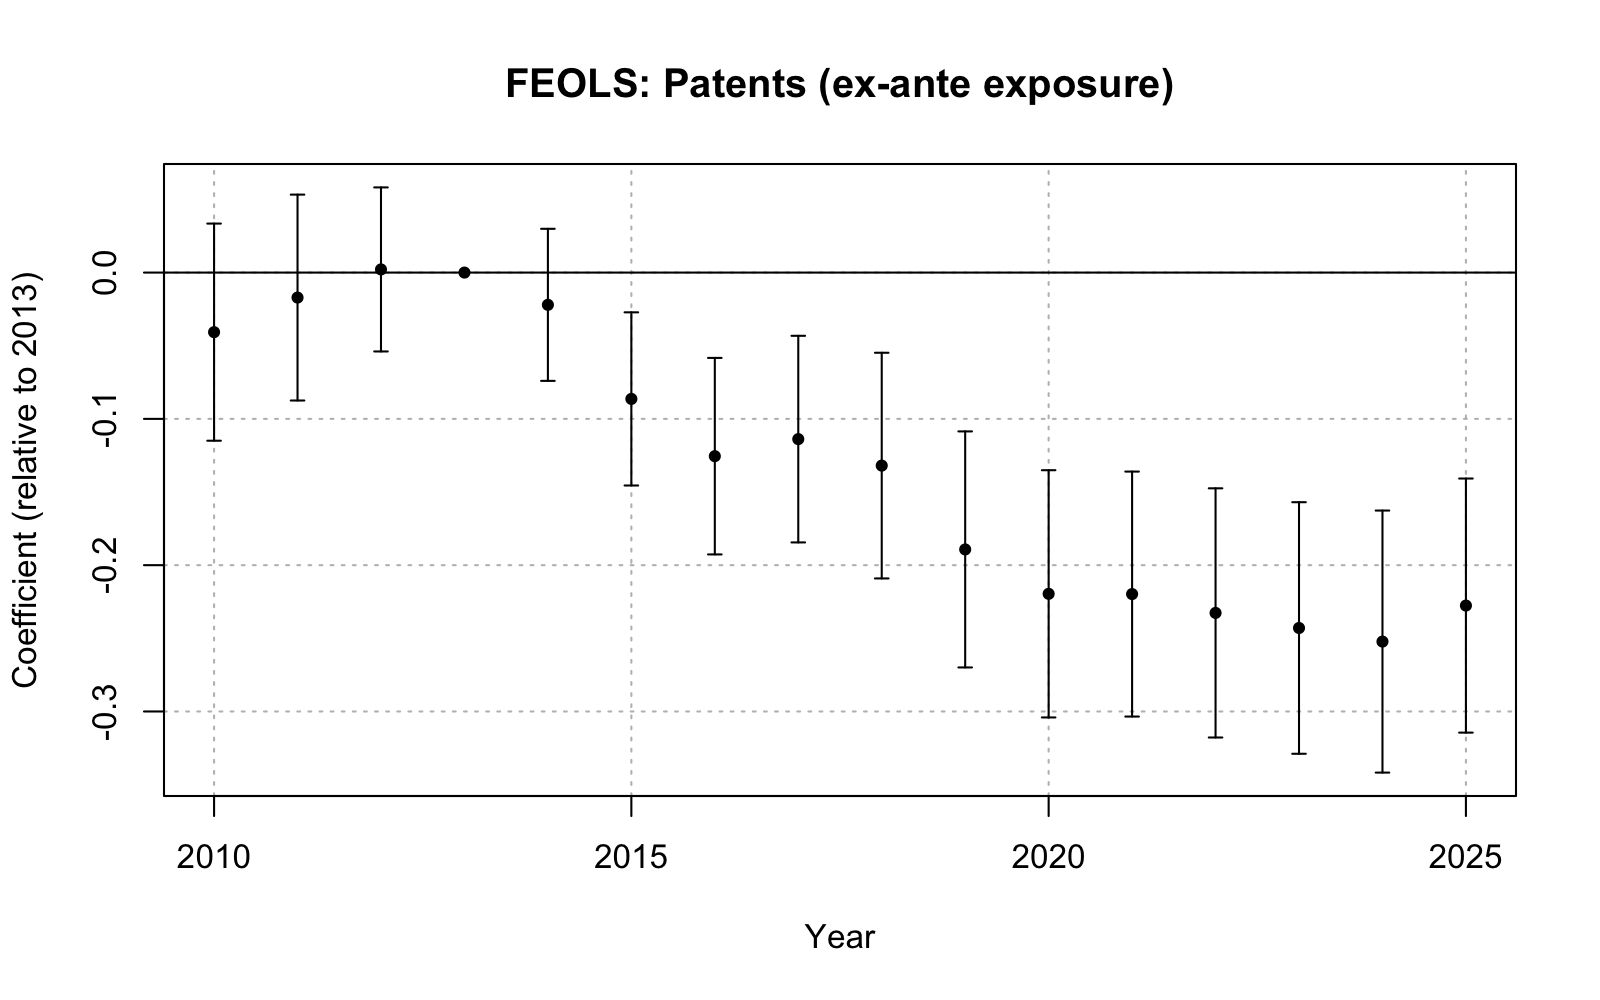
\includegraphics[width=\linewidth]{../output/RQ1/patent_feols_exante.png}
  \caption{FEOLS event study: patents, ex-ante Medicaid exposure}
  \label{fig:rq1_patent_feols_exante}
\end{figure}

\begin{figure}[!h]
  \centering
  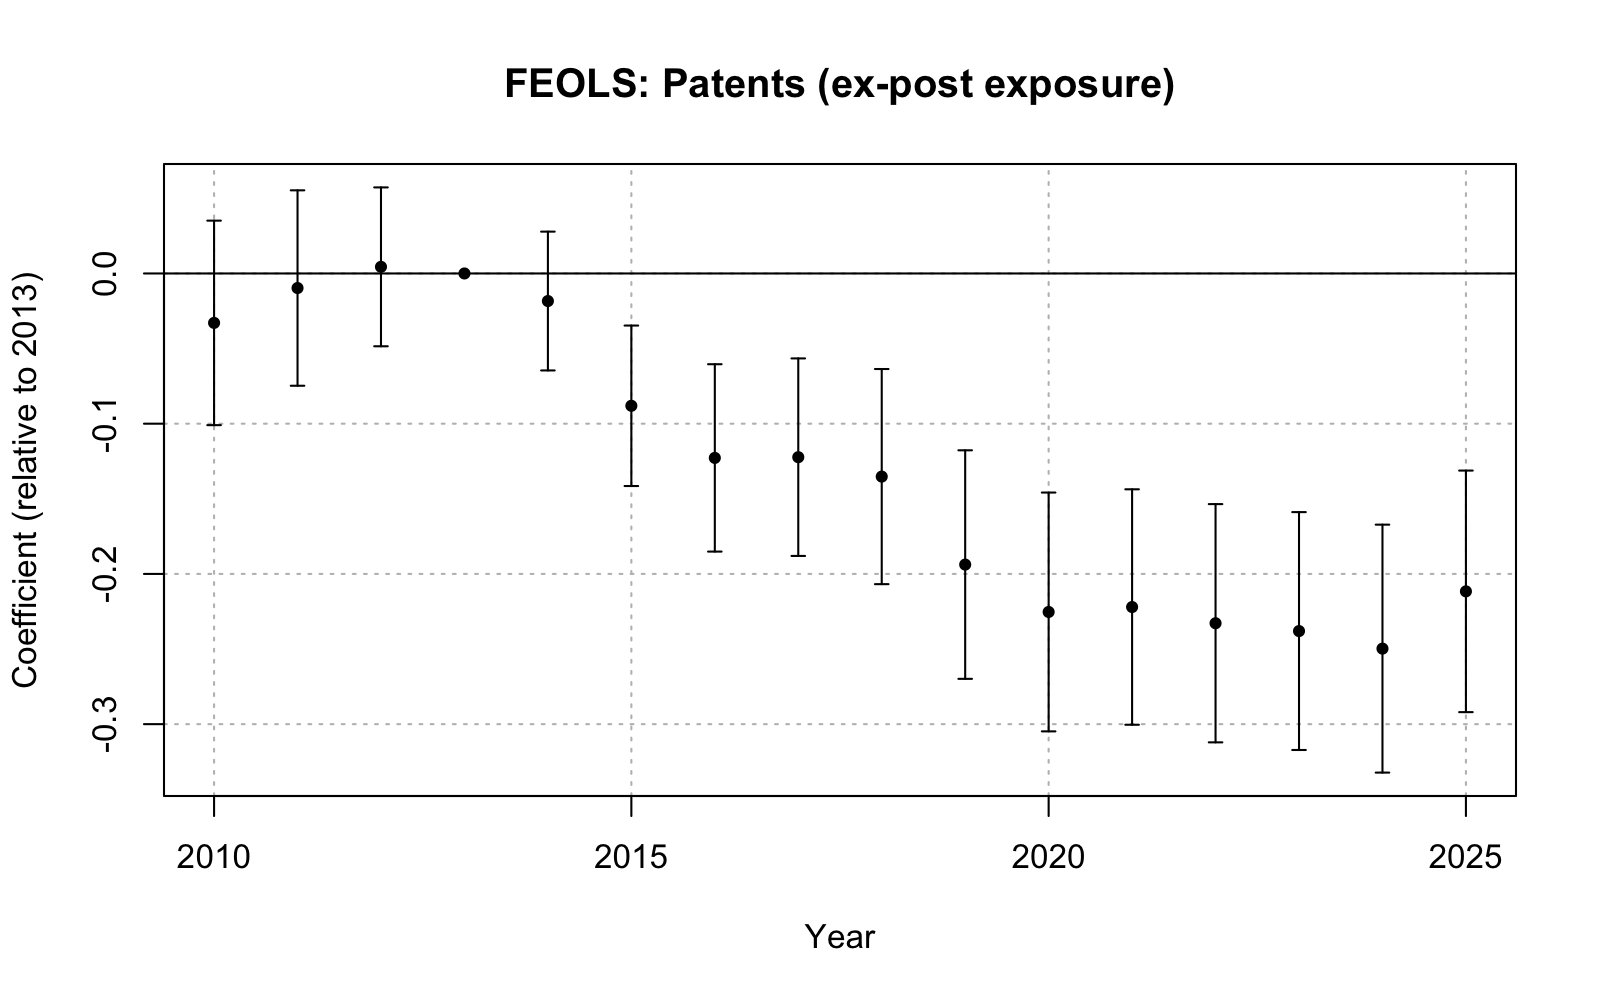
\includegraphics[width=\linewidth]{../output/RQ1/patent_feols_expost.png}
  \caption{FEOLS event study: patents, ex-post Medicaid exposure}
  \label{fig:rq1_patent_feols_expost}
\end{figure}

\begin{figure}[!h]
  \centering
  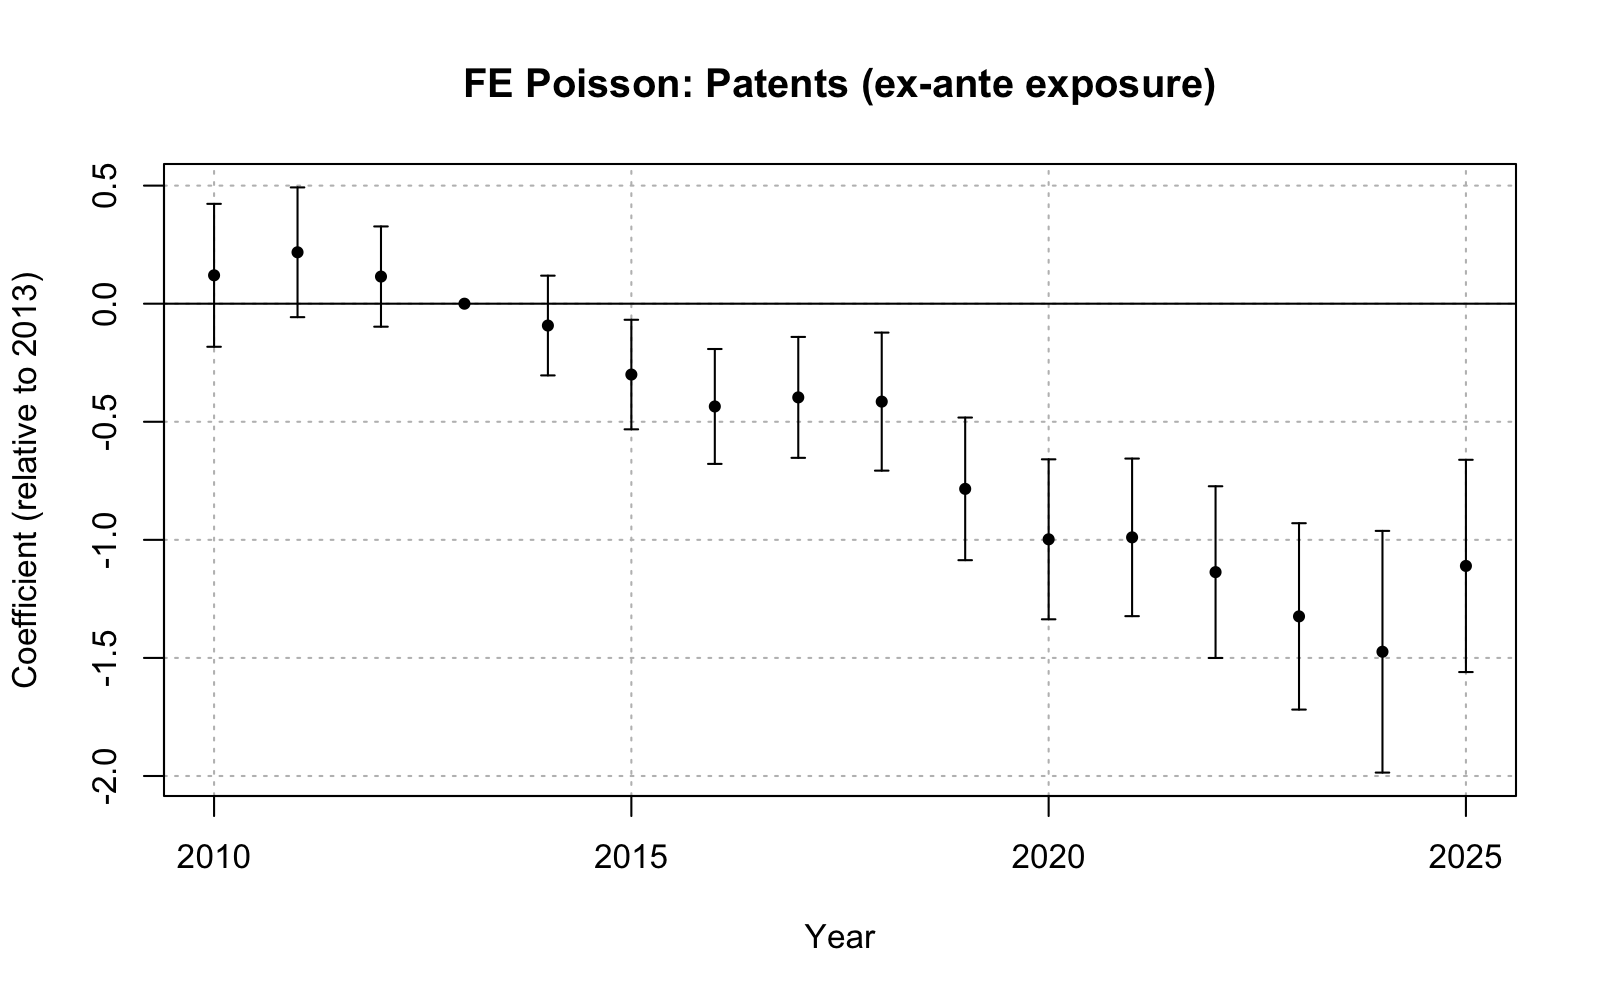
\includegraphics[width=\linewidth]{../output/RQ1/patent_poi_exante.png}
  \caption{FE Poisson event study: patents, ex-ante Medicaid exposure}
  \label{fig:rq1_patent_poi_exante}
\end{figure}

\begin{figure}[!h]
  \centering
  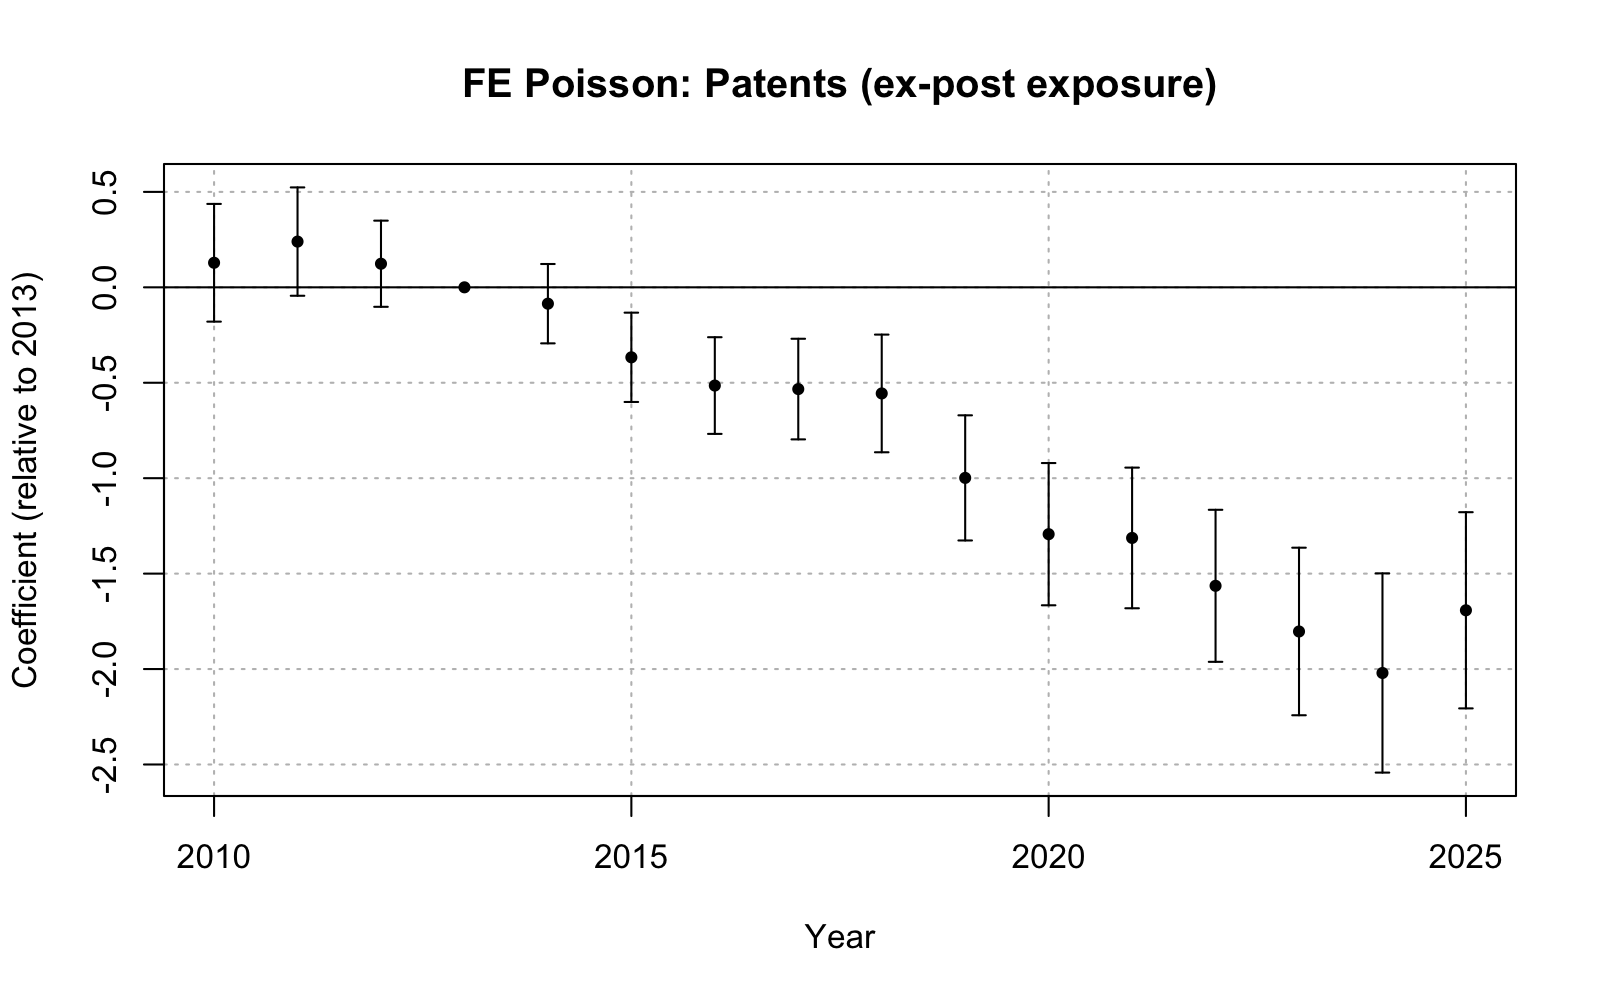
\includegraphics[width=\linewidth]{../output/RQ1/patent_poi_expost.png}
  \caption{FE Poisson event study: patents, ex-post Medicaid exposure}
  \label{fig:rq1_patent_poi_expost}
\end{figure}

\clearpage
\begingroup\footnotesize
\begin{table}
\centering
\begin{talltblr}[         %% tabularray outer open
entry=none,label=none,
note{}={* p \num{< 0.05}, ** p \num{< 0.01}, *** p \num{< 0.001}},
]                     %% tabularray outer close
{                     %% tabularray inner open
colspec={Q[]Q[]Q[]Q[]Q[]},
column{2,3,4,5}={}{halign=c,},
column{1}={}{halign=l,},
hline{32}={1,2,3,4,5}{solid, black, 0.05em},
}                     %% tabularray inner close
\toprule
& FEOLS: Ex Ante & FEOLS: Ex Post & FEPOIS: Ex Ante & FEPOIS: Ex Post \\ \midrule %% TinyTableHeader
2010 × medicaid\_market\_share & \num{-0.010}    & \num{-0.008}    & \num{0.120}     & \num{0.129}     \\
                                              & (\num{0.009})   & (\num{0.009})   & (\num{0.154})   & (\num{0.157})   \\
2011 × medicaid\_market\_share & \num{-0.004}    & \num{-0.002}    & \num{0.218}     & \num{0.240}     \\
                                              & (\num{0.009})   & (\num{0.008})   & (\num{0.140})   & (\num{0.145})   \\
2012 × medicaid\_market\_share & \num{0.001}     & \num{0.001}     & \num{0.115}     & \num{0.124}     \\
                                              & (\num{0.007})   & (\num{0.007})   & (\num{0.108})   & (\num{0.115})   \\
2014 × medicaid\_market\_share & \num{-0.006}    & \num{-0.005}    & \num{-0.092}    & \num{-0.086}    \\
                                              & (\num{0.007})   & (\num{0.006})   & (\num{0.108})   & (\num{0.106})   \\
2015 × medicaid\_market\_share & \num{-0.022}**  & \num{-0.022}**  & \num{-0.300}*   & \num{-0.367}**  \\
                                              & (\num{0.008})   & (\num{0.007})   & (\num{0.118})   & (\num{0.119})   \\
2016 × medicaid\_market\_share & \num{-0.031}*** & \num{-0.031}*** & \num{-0.435}*** & \num{-0.515}*** \\
                                              & (\num{0.009})   & (\num{0.008})   & (\num{0.124})   & (\num{0.129})   \\
2017 × medicaid\_market\_share & \num{-0.028}**  & \num{-0.031}*** & \num{-0.397}**  & \num{-0.533}*** \\
                                              & (\num{0.009})   & (\num{0.008})   & (\num{0.131})   & (\num{0.134})   \\
2018 × medicaid\_market\_share & \num{-0.033}*** & \num{-0.034}*** & \num{-0.415}**  & \num{-0.556}*** \\
                                              & (\num{0.010})   & (\num{0.009})   & (\num{0.149})   & (\num{0.157})   \\
2019 × medicaid\_market\_share & \num{-0.047}*** & \num{-0.048}*** & \num{-0.784}*** & \num{-0.998}*** \\
                                              & (\num{0.010})   & (\num{0.010})   & (\num{0.154})   & (\num{0.167})   \\
2020 × medicaid\_market\_share & \num{-0.055}*** & \num{-0.056}*** & \num{-0.998}*** & \num{-1.293}*** \\
                                              & (\num{0.011})   & (\num{0.010})   & (\num{0.173})   & (\num{0.190})   \\
2021 × medicaid\_market\_share & \num{-0.055}*** & \num{-0.056}*** & \num{-0.989}*** & \num{-1.313}*** \\
                                              & (\num{0.011})   & (\num{0.010})   & (\num{0.170})   & (\num{0.188})   \\
2022 × medicaid\_market\_share & \num{-0.058}*** & \num{-0.058}*** & \num{-1.137}*** & \num{-1.564}*** \\
                                              & (\num{0.011})   & (\num{0.010})   & (\num{0.186})   & (\num{0.203})   \\
2023 × medicaid\_market\_share & \num{-0.061}*** & \num{-0.060}*** & \num{-1.324}*** & \num{-1.803}*** \\
                                              & (\num{0.011})   & (\num{0.010})   & (\num{0.201})   & (\num{0.224})   \\
2024 × medicaid\_market\_share & \num{-0.063}*** & \num{-0.062}*** & \num{-1.474}*** & \num{-2.021}*** \\
                                              & (\num{0.011})   & (\num{0.011})   & (\num{0.261})   & (\num{0.266})   \\
2025 × medicaid\_market\_share & \num{-0.057}*** & \num{-0.053}*** & \num{-1.110}*** & \num{-1.692}*** \\
                                              & (\num{0.011})   & (\num{0.010})   & (\num{0.229})   & (\num{0.262})   \\
Num. obs.                                     & \num{21126784}  & \num{21126784}  & \num{5203776}   & \num{5203776}   \\
R2                                            & \num{0.392}     & \num{0.392}     &                 &                 \\
\bottomrule
\end{talltblr}
\end{table}

\endgroup

\clearpage

\subsection{FDA Approvals}

\begin{figure}[!h]
  \centering
  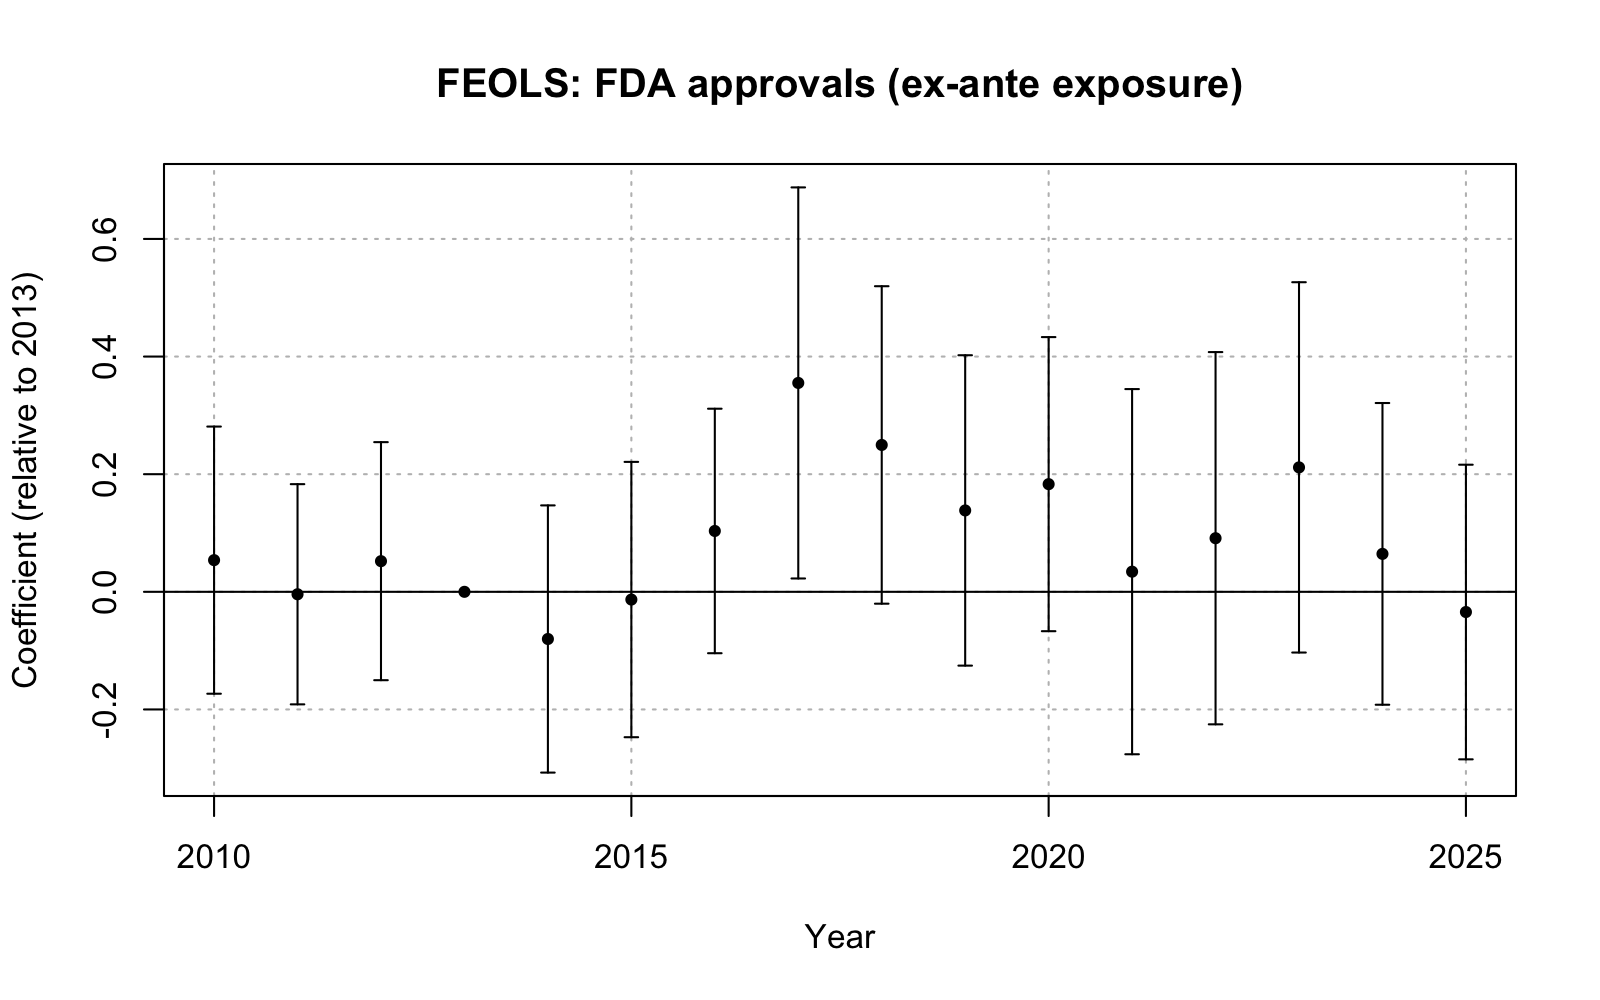
\includegraphics[width=\linewidth]{../output/RQ1/fda_feols_exante.png}
  \caption{FEOLS event study: FDA approvals, ex-ante Medicaid exposure}
  \label{fig:rq1_fda_feols_exante}
\end{figure}

\begin{figure}[!h]
  \centering
  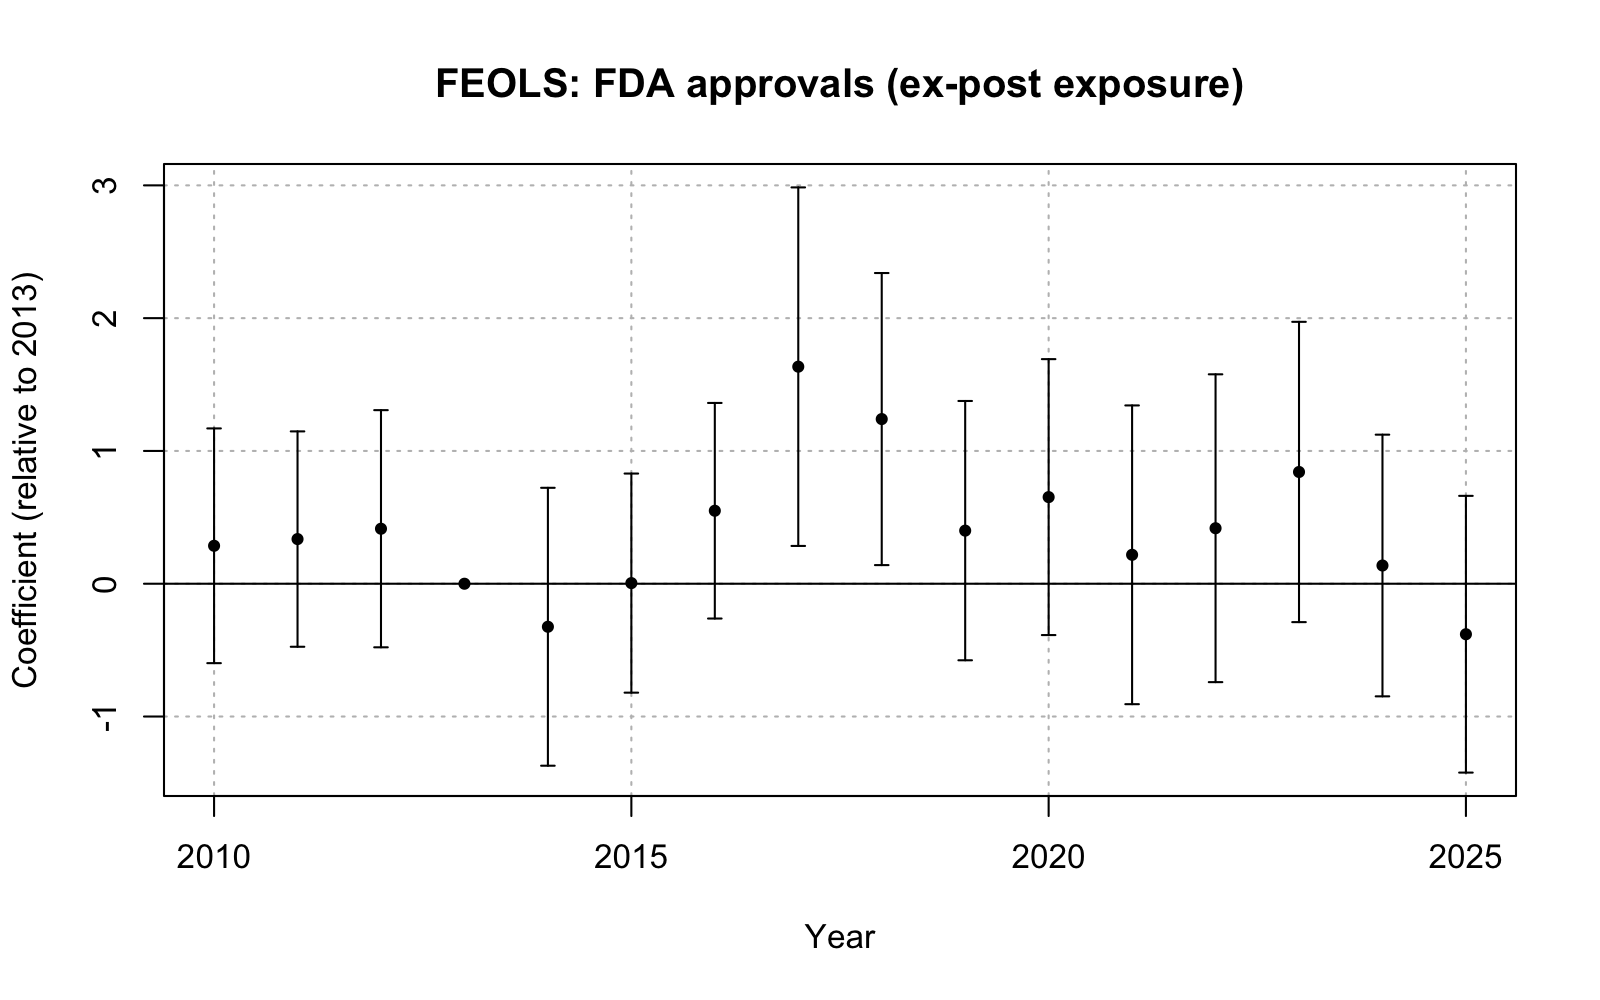
\includegraphics[width=\linewidth]{../output/RQ1/fda_feols_expost.png}
  \caption{FEOLS event study: FDA approvals, ex-post Medicaid exposure}
  \label{fig:rq1_fda_feols_expost}
\end{figure}

\begin{figure}[!h]
  \centering
  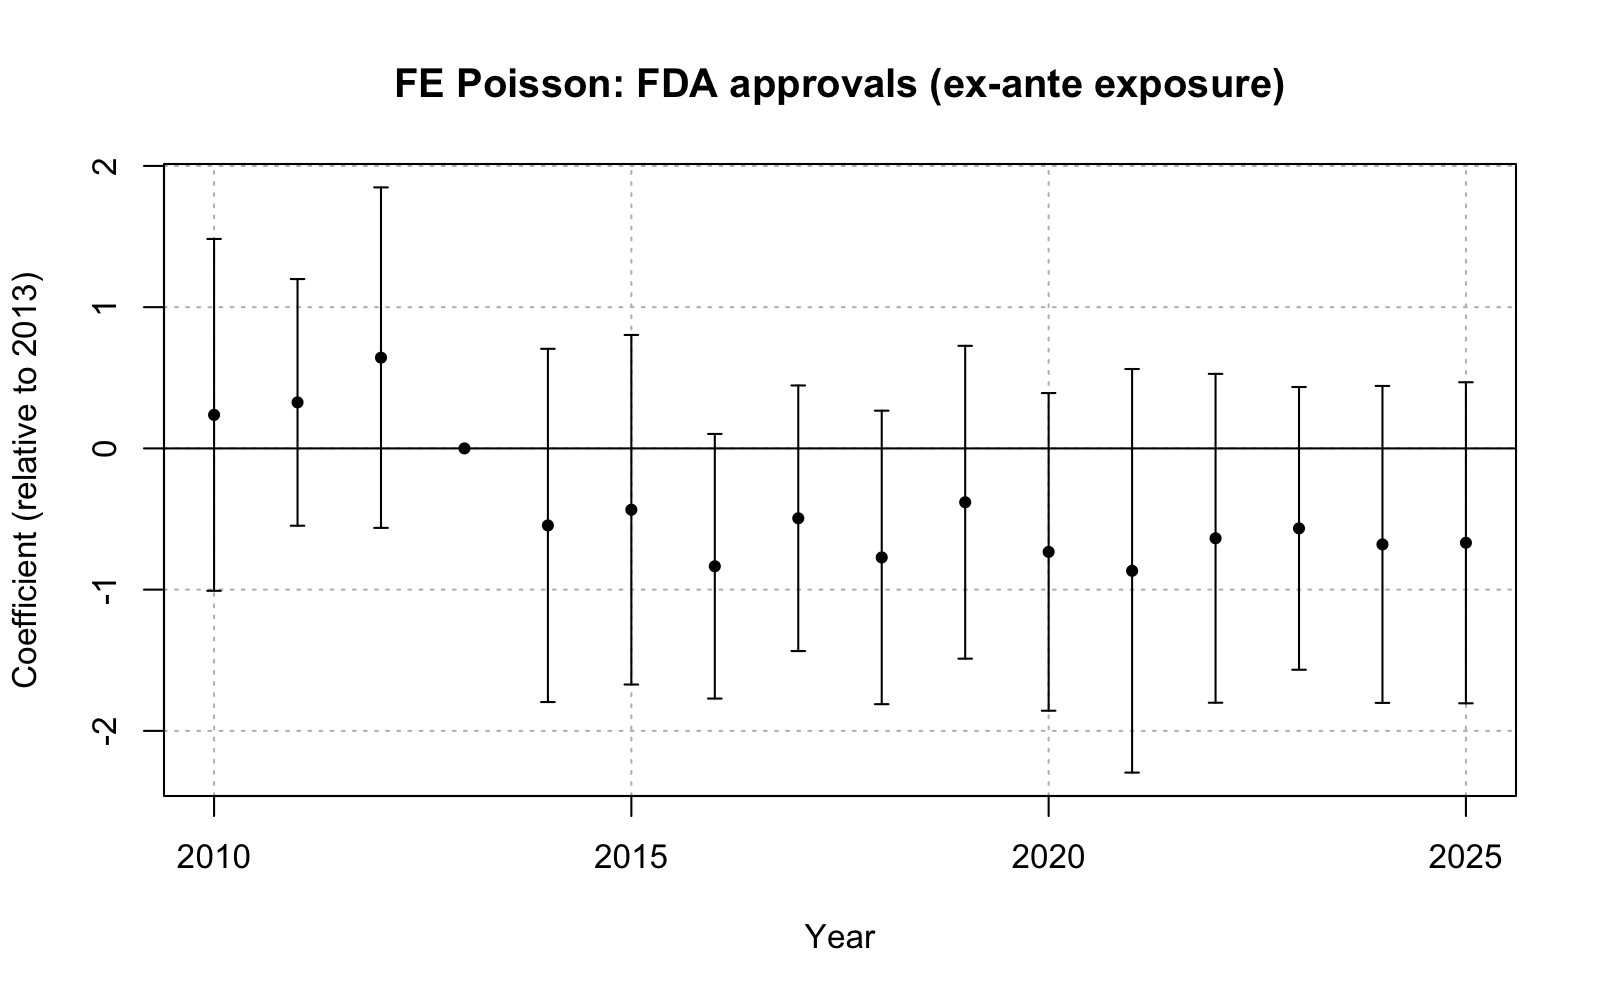
\includegraphics[width=\linewidth]{../output/RQ1/fda_poi_exante.png}
  \caption{FE Poisson event study: FDA approvals, ex-ante Medicaid exposure}
  \label{fig:rq1_fda_poi_exante}
\end{figure}

\begin{figure}[!h]
  \centering
  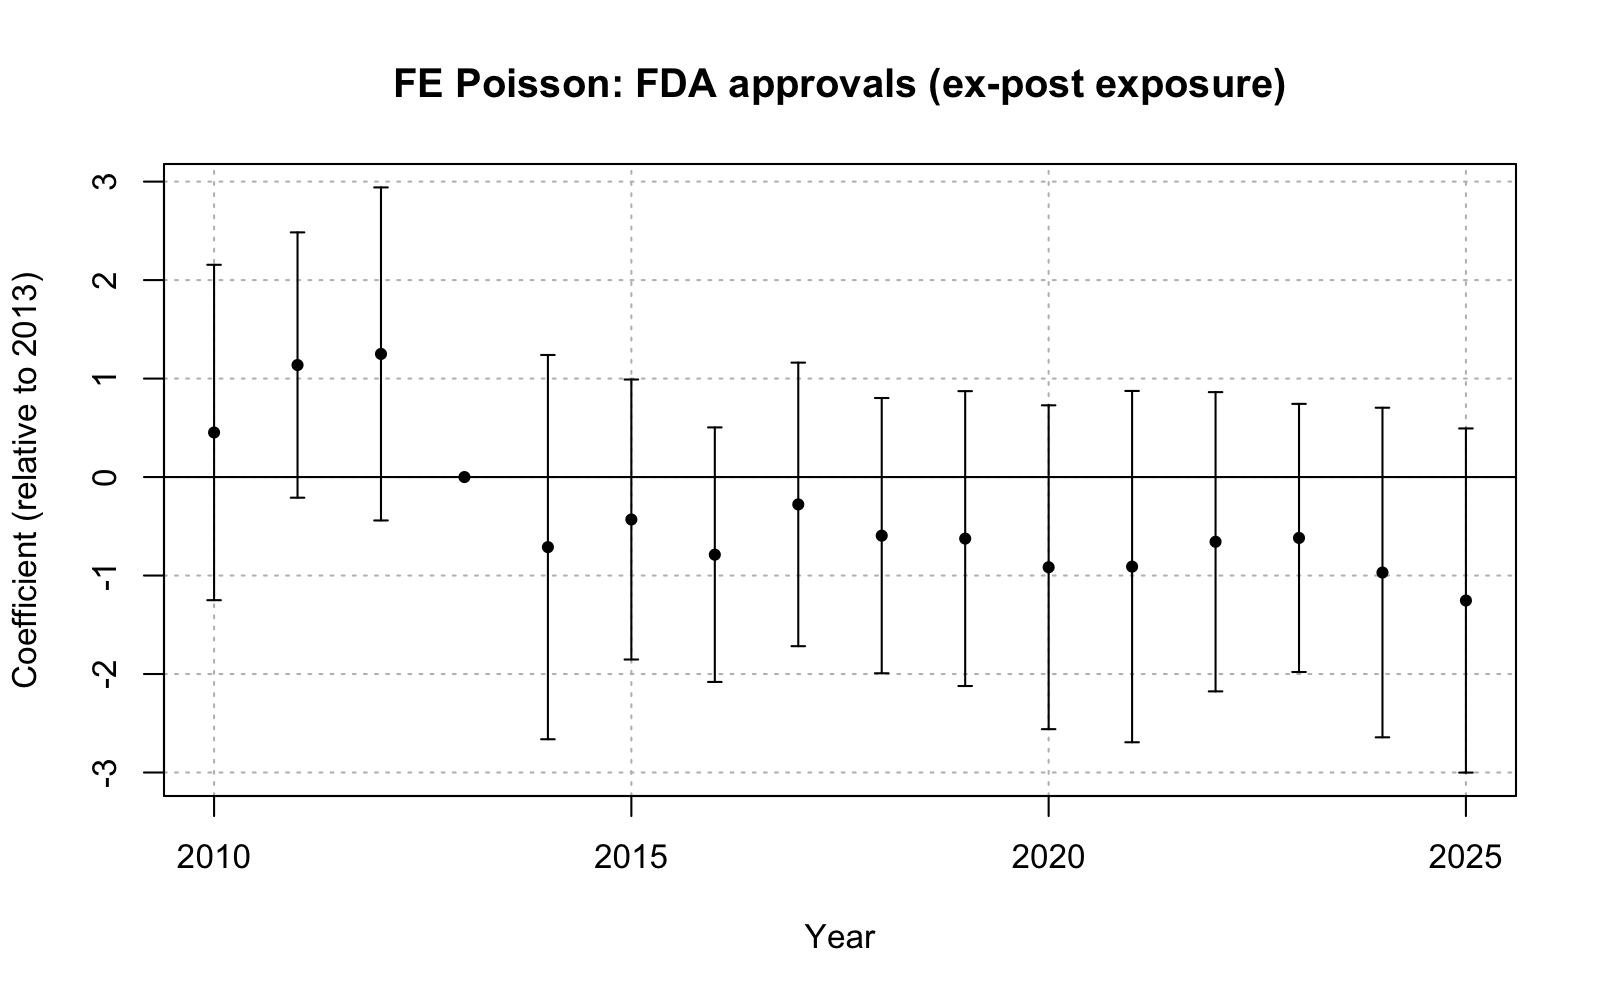
\includegraphics[width=\linewidth]{../output/RQ1/fda_poi_expost.png}
  \caption{FE Poisson event study: FDA approvals, ex-post Medicaid exposure}
  \label{fig:rq1_fda_poi_expost}
\end{figure}

\clearpage
\begingroup\footnotesize
\begin{table}
\centering
\begin{talltblr}[         %% tabularray outer open
entry=none,label=none,
note{}={* p \num{< 0.05}, ** p \num{< 0.01}, *** p \num{< 0.001}},
]                     %% tabularray outer close
{                     %% tabularray inner open
colspec={Q[]Q[]Q[]Q[]Q[]},
column{2,3,4,5}={}{halign=c,},
column{1}={}{halign=l,},
hline{32}={1,2,3,4,5}{solid, black, 0.05em},
}                     %% tabularray inner close
\toprule
& FEOLS: Ex Ante & FEOLS: Ex Post & FEPOIS: Ex Ante & FEPOIS: Ex Post \\ \midrule %% TinyTableHeader
2010 × medicaid\_market\_share & \num{0.054}   & \num{0.071}   & \num{0.237}   & \num{0.453}   \\
& (\num{0.116}) & (\num{0.113}) & (\num{0.636}) & (\num{0.869}) \\
2011 × medicaid\_market\_share & \num{-0.004}  & \num{0.084}   & \num{0.326}   & \num{1.138}   \\
& (\num{0.095}) & (\num{0.103}) & (\num{0.446}) & (\num{0.687}) \\
2012 × medicaid\_market\_share & \num{0.052}   & \num{0.104}   & \num{0.643}   & \num{1.250}   \\
& (\num{0.103}) & (\num{0.114}) & (\num{0.615}) & (\num{0.863}) \\
2014 × medicaid\_market\_share & \num{-0.080}  & \num{-0.081}  & \num{-0.545}  & \num{-0.711}  \\
& (\num{0.116}) & (\num{0.133}) & (\num{0.638}) & (\num{0.995}) \\
2015 × medicaid\_market\_share & \num{-0.013}  & \num{0.001}   & \num{-0.434}  & \num{-0.431}  \\
& (\num{0.119}) & (\num{0.105}) & (\num{0.631}) & (\num{0.725}) \\
2016 × medicaid\_market\_share & \num{0.103}   & \num{0.137}   & \num{-0.834}  & \num{-0.788}  \\
& (\num{0.106}) & (\num{0.103}) & (\num{0.478}) & (\num{0.659}) \\
2017 × medicaid\_market\_share & \num{0.355}*  & \num{0.409}*  & \num{-0.495}  & \num{-0.278}  \\
& (\num{0.169}) & (\num{0.172}) & (\num{0.480}) & (\num{0.735}) \\
2018 × medicaid\_market\_share & \num{0.250}   & \num{0.310}*  & \num{-0.772}  & \num{-0.595}  \\
& (\num{0.137}) & (\num{0.140}) & (\num{0.530}) & (\num{0.713}) \\
2019 × medicaid\_market\_share & \num{0.138}   & \num{0.100}   & \num{-0.381}  & \num{-0.625}  \\
& (\num{0.134}) & (\num{0.124}) & (\num{0.565}) & (\num{0.764}) \\
2020 × medicaid\_market\_share & \num{0.183}   & \num{0.163}   & \num{-0.733}  & \num{-0.916}  \\
& (\num{0.127}) & (\num{0.132}) & (\num{0.574}) & (\num{0.839}) \\
2021 × medicaid\_market\_share & \num{0.034}   & \num{0.054}   & \num{-0.867}  & \num{-0.909}  \\
& (\num{0.158}) & (\num{0.143}) & (\num{0.729}) & (\num{0.910}) \\
2022 × medicaid\_market\_share & \num{0.091}   & \num{0.104}   & \num{-0.637}  & \num{-0.657}  \\
& (\num{0.161}) & (\num{0.148}) & (\num{0.594}) & (\num{0.775}) \\
2023 × medicaid\_market\_share & \num{0.212}   & \num{0.210}   & \num{-0.566}  & \num{-0.618}  \\
& (\num{0.160}) & (\num{0.144}) & (\num{0.511}) & (\num{0.695}) \\
2024 × medicaid\_market\_share & \num{0.065}   & \num{0.034}   & \num{-0.680}  & \num{-0.969}  \\
& (\num{0.131}) & (\num{0.125}) & (\num{0.573}) & (\num{0.854}) \\
2025 × medicaid\_market\_share & \num{-0.034}  & \num{-0.095}  & \num{-0.668}  & \num{-1.254}  \\
& (\num{0.128}) & (\num{0.133}) & (\num{0.580}) & (\num{0.892}) \\
Num. obs.                                          & \num{604800}  & \num{604800}  & \num{168704}  & \num{168704}  \\
R2                                                 & \num{0.314}   & \num{0.314}   &                &                \\
\bottomrule
\end{talltblr}
\end{table}

\endgroup

\clearpage

% -----------------------------------------------------------------------
\section{RQ2: Medicaid Demand and PDL Exposure}
% -----------------------------------------------------------------------

\subsection{Patents}

\begin{figure}[!h]
  \centering
  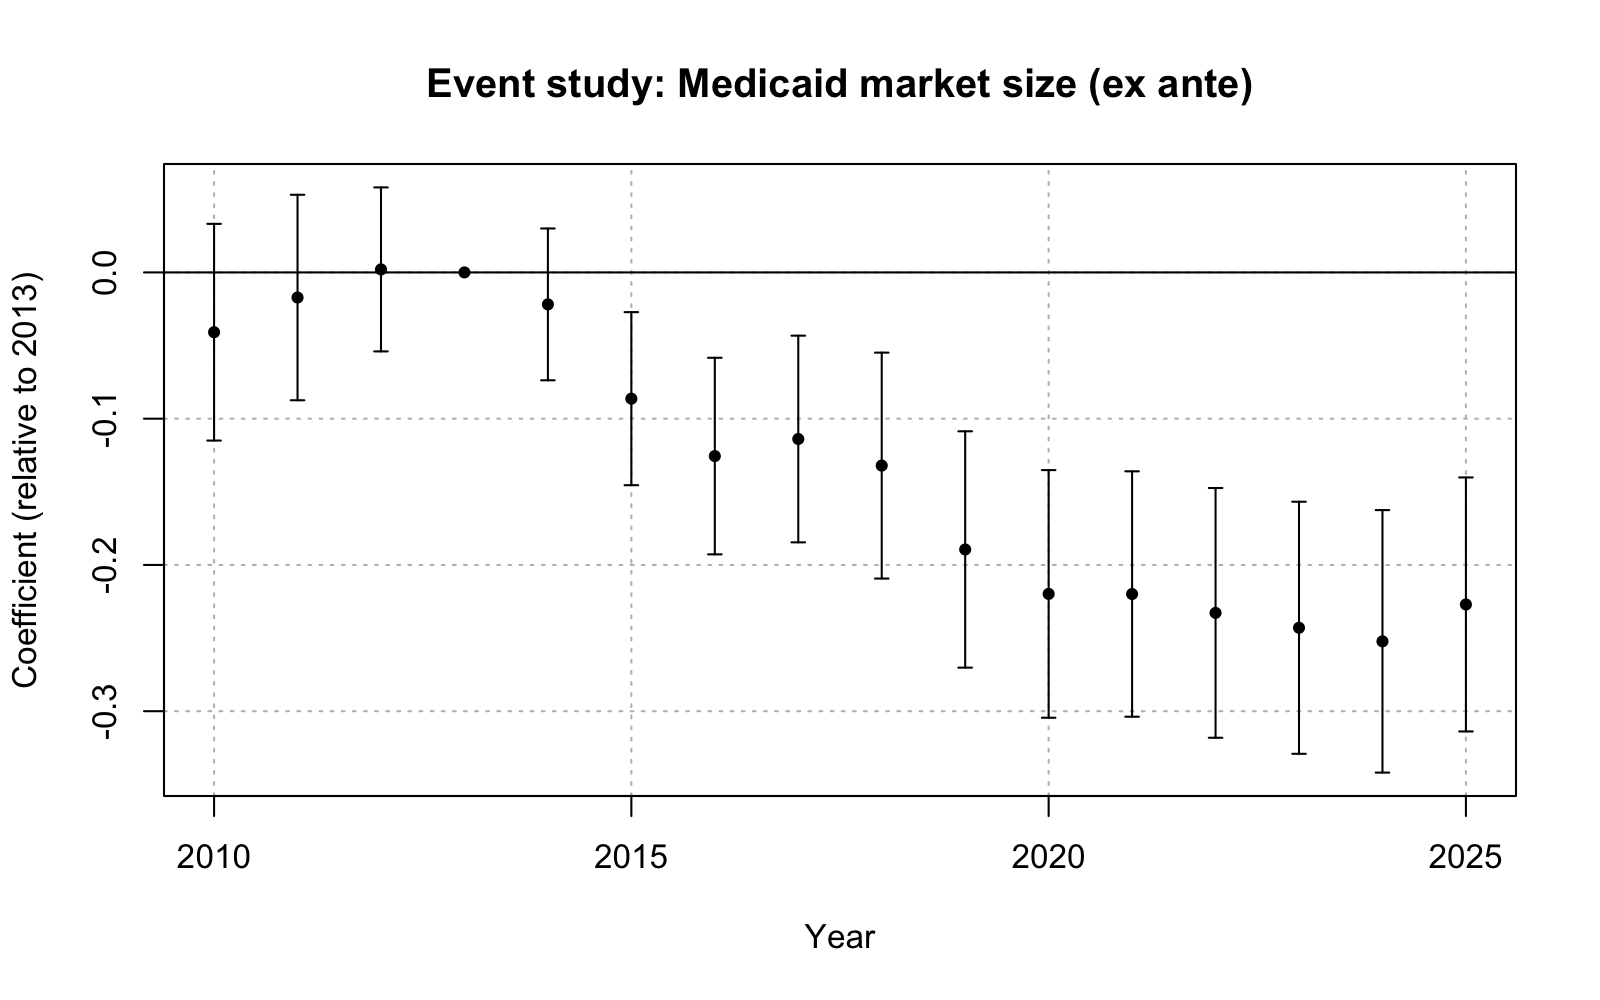
\includegraphics[width=\linewidth]{../output/RQ2/patent_feols_exante_medicaid.png}
  \caption{FEOLS event study: patents, Medicaid exposure (ex-ante)}
  \label{fig:rq2_patent_feols_exante_medicaid}
\end{figure}

\begin{figure}[!h]
  \centering
  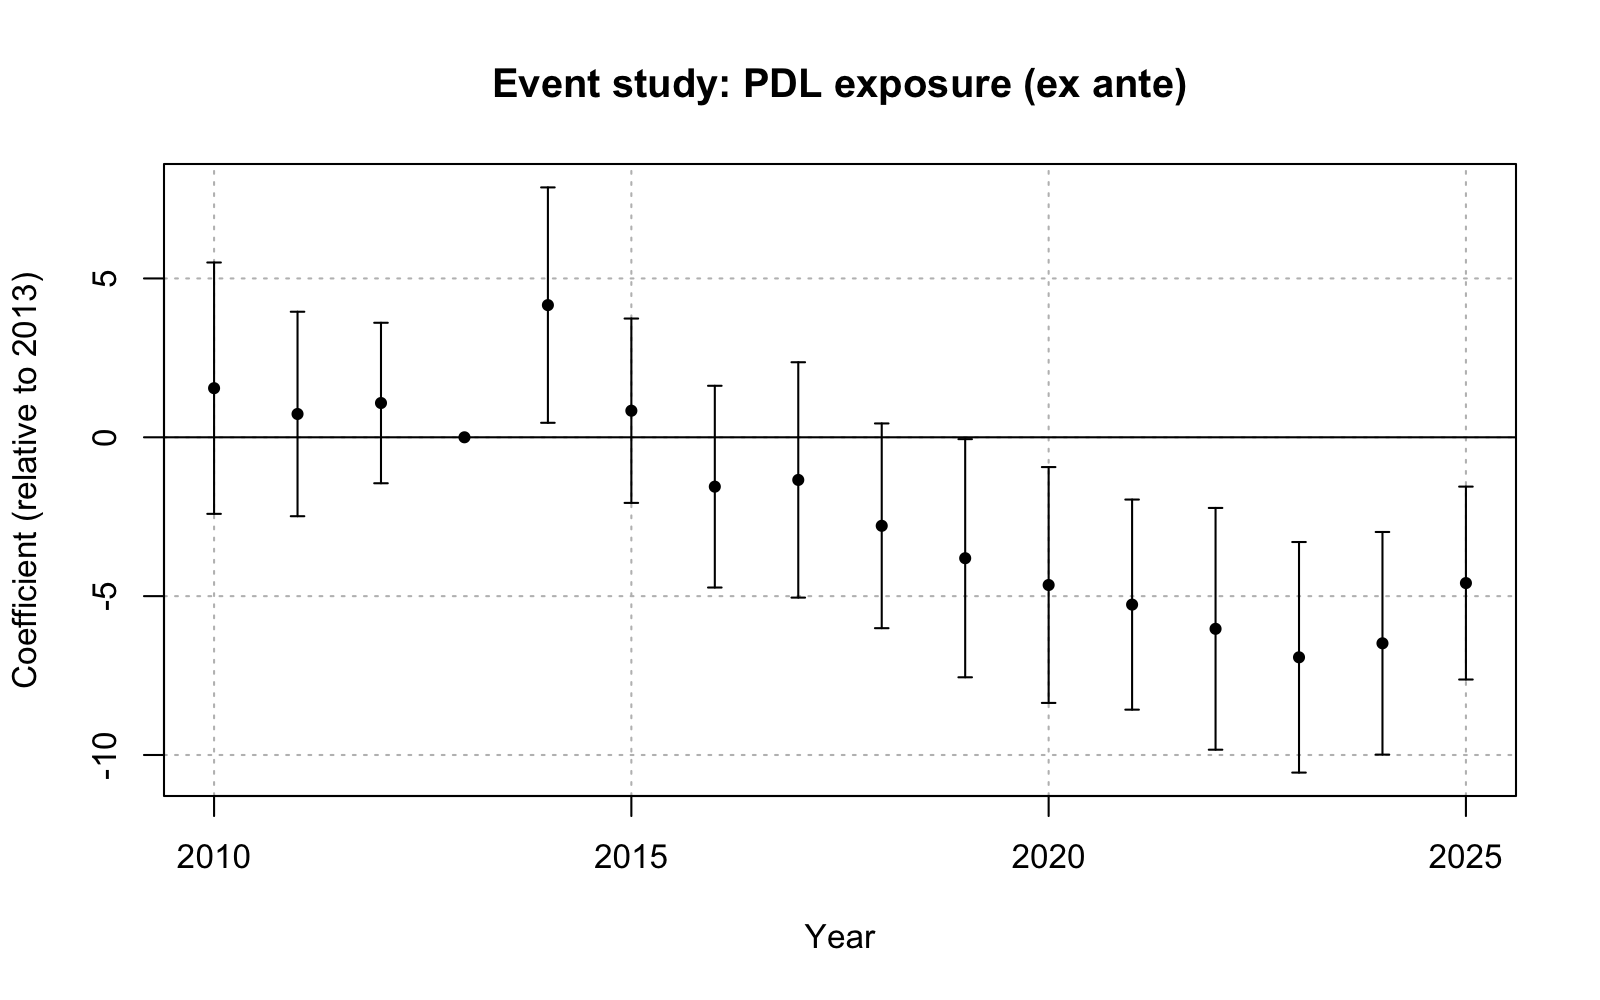
\includegraphics[width=\linewidth]{../output/RQ2/patent_feols_exante_pdl.png}
  \caption{FEOLS event study: patents, PDL exposure (ex-ante)}
  \label{fig:rq2_patent_feols_exante_pdl}
\end{figure}

\begin{figure}[!h]
  \centering
  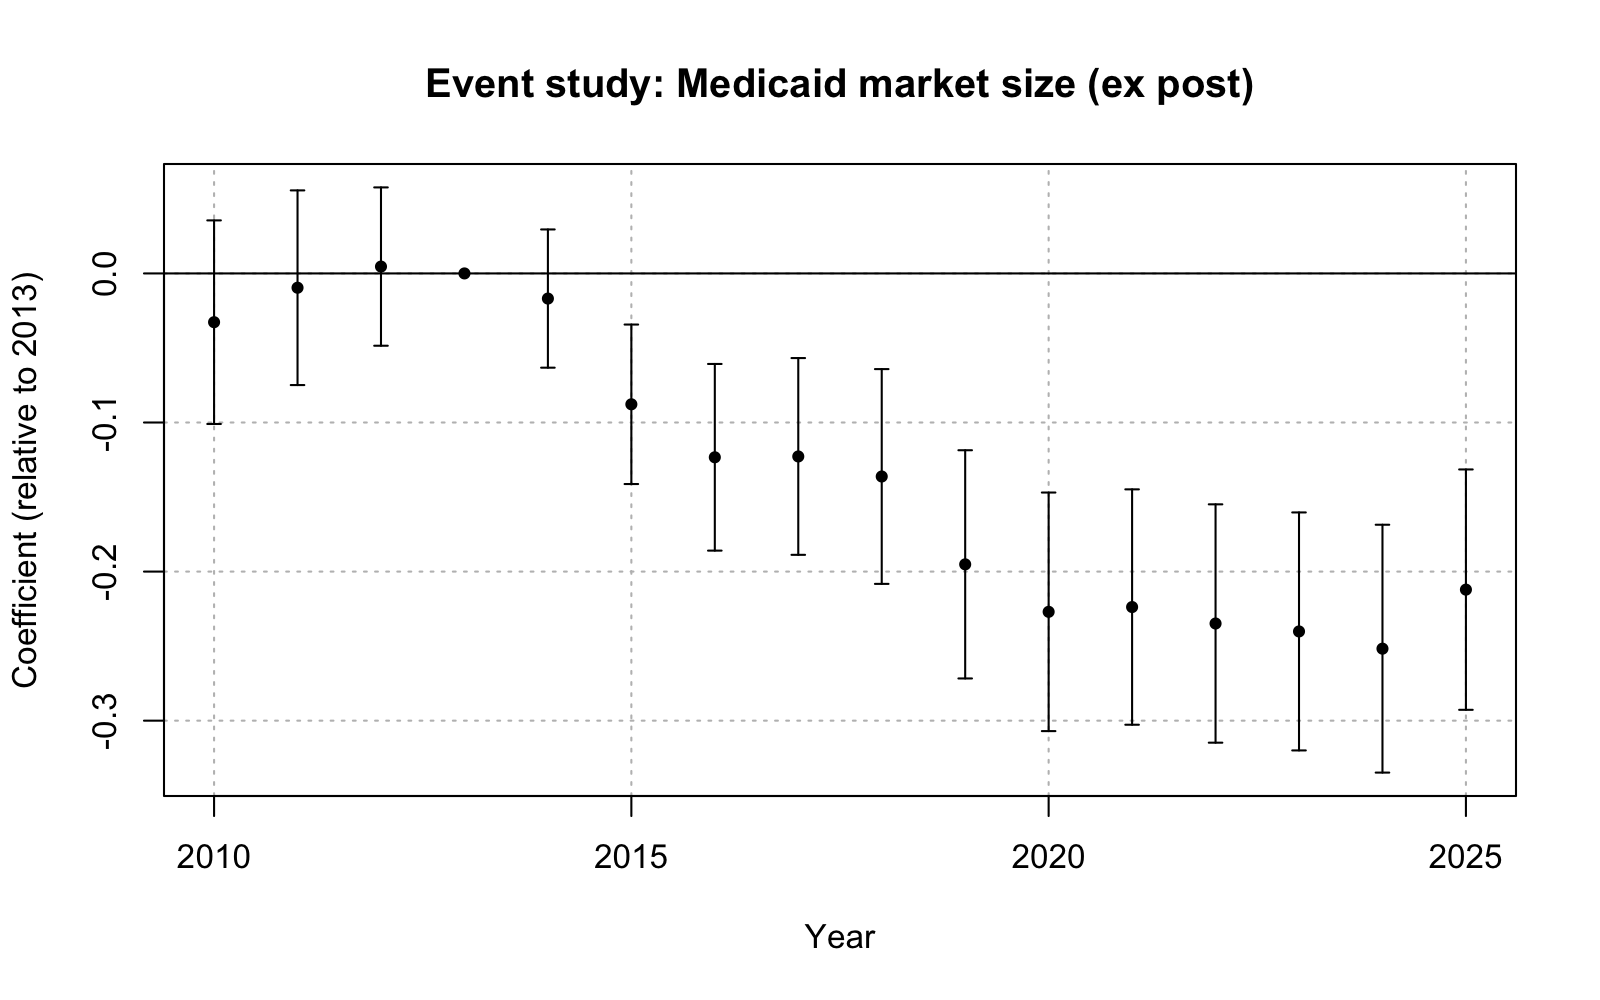
\includegraphics[width=\linewidth]{../output/RQ2/patent_feols_expost_medicaid.png}
  \caption{FEOLS event study: patents, Medicaid exposure (ex-post)}
  \label{fig:rq2_patent_feols_expost_medicaid}
\end{figure}

\begin{figure}[!h]
  \centering
  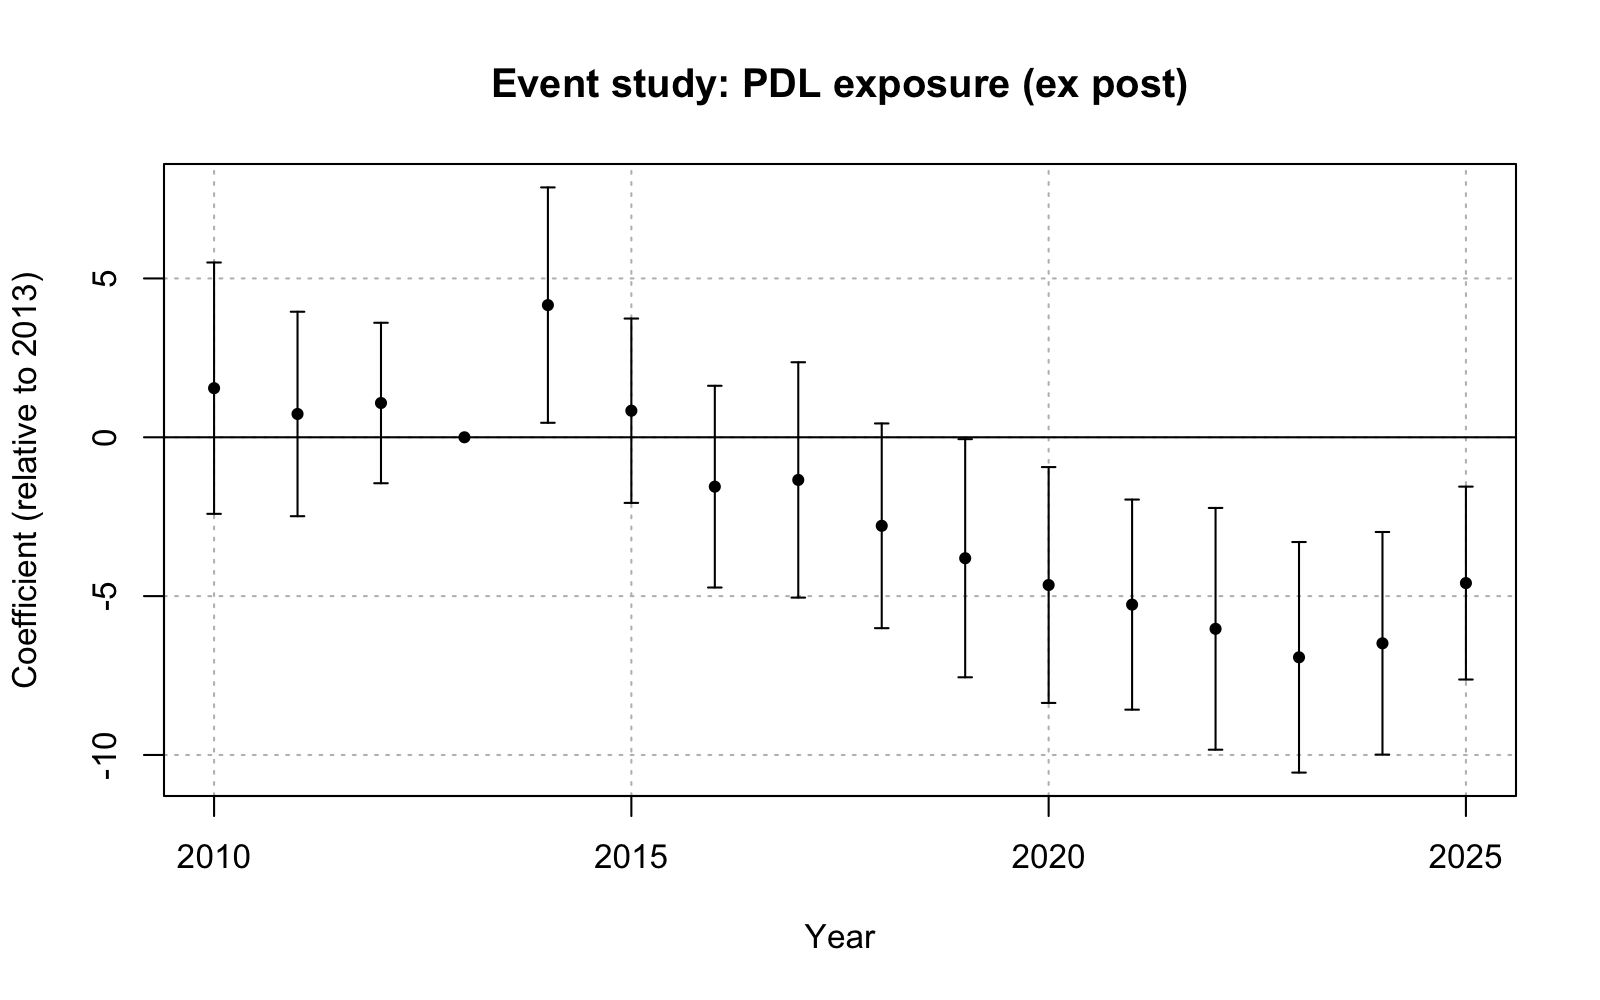
\includegraphics[width=\linewidth]{../output/RQ2/patent_feols_expost_pdl.png}
  \caption{FEOLS event study: patents, PDL exposure (ex-post)}
  \label{fig:rq2_patent_feols_expost_pdl}
\end{figure}

\clearpage
\begingroup\footnotesize
\begin{table}
\centering
\begin{talltblr}[         %% tabularray outer open
entry=none,label=none,
note{}={* p \num{< 0.05}, ** p \num{< 0.01}, *** p \num{< 0.001}},
]                     %% tabularray outer close
{                     %% tabularray inner open
colspec={Q[]Q[]Q[]},
column{2,3}={}{halign=c,},
column{1}={}{halign=l,},
hline{62}={1,2,3}{solid, black, 0.05em},
}                     %% tabularray inner close
\toprule
& FEOLS: Ex Ante & FEOLS: Ex Post \\ \midrule %% TinyTableHeader
2010 × medicaid\_market\_share & \num{-0.041}    & \num{-0.033}    \\
& (\num{0.038})   & (\num{0.035})   \\
2011 × medicaid\_market\_share & \num{-0.017}    & \num{-0.010}    \\
& (\num{0.036})   & (\num{0.033})   \\
2012 × medicaid\_market\_share & \num{0.002}     & \num{0.005}     \\
& (\num{0.029})   & (\num{0.027})   \\
2014 × medicaid\_market\_share & \num{-0.022}    & \num{-0.017}    \\
& (\num{0.026})   & (\num{0.024})   \\
2015 × medicaid\_market\_share & \num{-0.086}**  & \num{-0.088}**  \\
& (\num{0.030})   & (\num{0.027})   \\
2016 × medicaid\_market\_share & \num{-0.126}*** & \num{-0.123}*** \\
& (\num{0.034})   & (\num{0.032})   \\
2017 × medicaid\_market\_share & \num{-0.114}**  & \num{-0.123}*** \\
& (\num{0.036})   & (\num{0.034})   \\
2018 × medicaid\_market\_share & \num{-0.132}*** & \num{-0.136}*** \\
& (\num{0.039})   & (\num{0.037})   \\
2019 × medicaid\_market\_share & \num{-0.189}*** & \num{-0.195}*** \\
& (\num{0.041})   & (\num{0.039})   \\
2020 × medicaid\_market\_share & \num{-0.220}*** & \num{-0.227}*** \\
& (\num{0.043})   & (\num{0.041})   \\
2021 × medicaid\_market\_share & \num{-0.220}*** & \num{-0.224}*** \\
& (\num{0.043})   & (\num{0.040})   \\
2022 × medicaid\_market\_share & \num{-0.233}*** & \num{-0.235}*** \\
& (\num{0.044})   & (\num{0.041})   \\
2023 × medicaid\_market\_share & \num{-0.243}*** & \num{-0.240}*** \\
& (\num{0.044})   & (\num{0.041})   \\
2024 × medicaid\_market\_share & \num{-0.252}*** & \num{-0.252}*** \\
& (\num{0.046})   & (\num{0.042})   \\
2025 × medicaid\_market\_share & \num{-0.227}*** & \num{-0.212}*** \\
& (\num{0.044})   & (\num{0.041})   \\
2010 × in\_pdl                  & \num{1.546}     & \num{1.546}     \\
& (\num{2.018})   & (\num{2.018})   \\
2011 × in\_pdl                  & \num{0.734}     & \num{0.734}     \\
& (\num{1.642})   & (\num{1.642})   \\
2012 × in\_pdl                  & \num{1.079}     & \num{1.079}     \\
& (\num{1.289})   & (\num{1.289})   \\
2014 × in\_pdl                  & \num{4.161}*    & \num{4.161}*    \\
& (\num{1.890})   & (\num{1.890})   \\
2015 × in\_pdl                  & \num{0.836}     & \num{0.836}     \\
& (\num{1.480})   & (\num{1.480})   \\
2016 × in\_pdl                  & \num{-1.554}    & \num{-1.554}    \\
& (\num{1.620})   & (\num{1.620})   \\
2017 × in\_pdl                  & \num{-1.342}    & \num{-1.342}    \\
& (\num{1.890})   & (\num{1.890})   \\
2018 × in\_pdl                  & \num{-2.786}    & \num{-2.787}    \\
& (\num{1.644})   & (\num{1.644})   \\
2019 × in\_pdl                  & \num{-3.806}*   & \num{-3.807}*   \\
& (\num{1.912})   & (\num{1.912})   \\
2020 × in\_pdl                  & \num{-4.649}*   & \num{-4.650}*   \\
& (\num{1.894})   & (\num{1.894})   \\
2021 × in\_pdl                  & \num{-5.266}**  & \num{-5.267}**  \\
& (\num{1.687})   & (\num{1.687})   \\
2022 × in\_pdl                  & \num{-6.029}**  & \num{-6.029}**  \\
& (\num{1.941})   & (\num{1.941})   \\
2023 × in\_pdl                  & \num{-6.925}*** & \num{-6.926}*** \\
& (\num{1.851})   & (\num{1.851})   \\
2024 × in\_pdl                  & \num{-6.484}*** & \num{-6.485}*** \\
& (\num{1.788})   & (\num{1.788})   \\
2025 × in\_pdl                  & \num{-4.588}**  & \num{-4.589}**  \\
& (\num{1.549})   & (\num{1.549})   \\
Num. obs.                                        & \num{5281696}   & \num{5281696}   \\
R2                                               & \num{0.535}     & \num{0.535}     \\
\bottomrule
\end{talltblr}
\end{table}

\endgroup

\clearpage

\subsection{FDA Approvals}

\begin{figure}[!h]
  \centering
  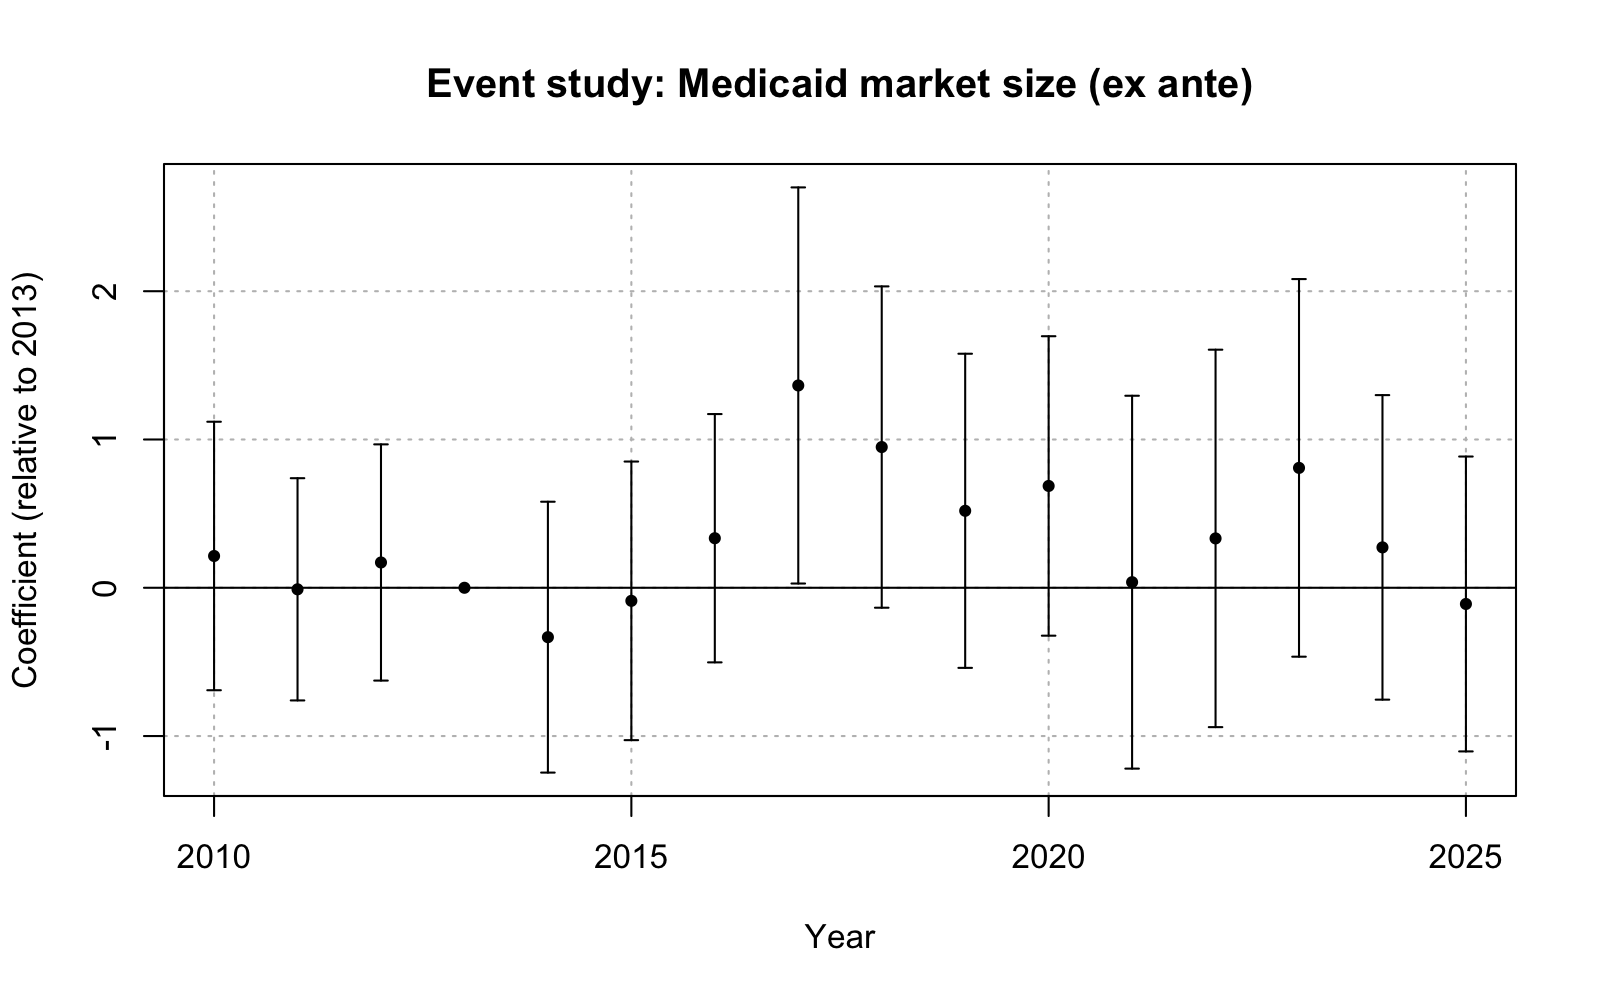
\includegraphics[width=\linewidth]{../output/RQ2/fda_feols_exante_medicaid.png}
  \caption{FEOLS event study: FDA approvals, Medicaid exposure (ex-ante)}
  \label{fig:rq2_fda_feols_exante_medicaid}
\end{figure}

\begin{figure}[!h]
  \centering
  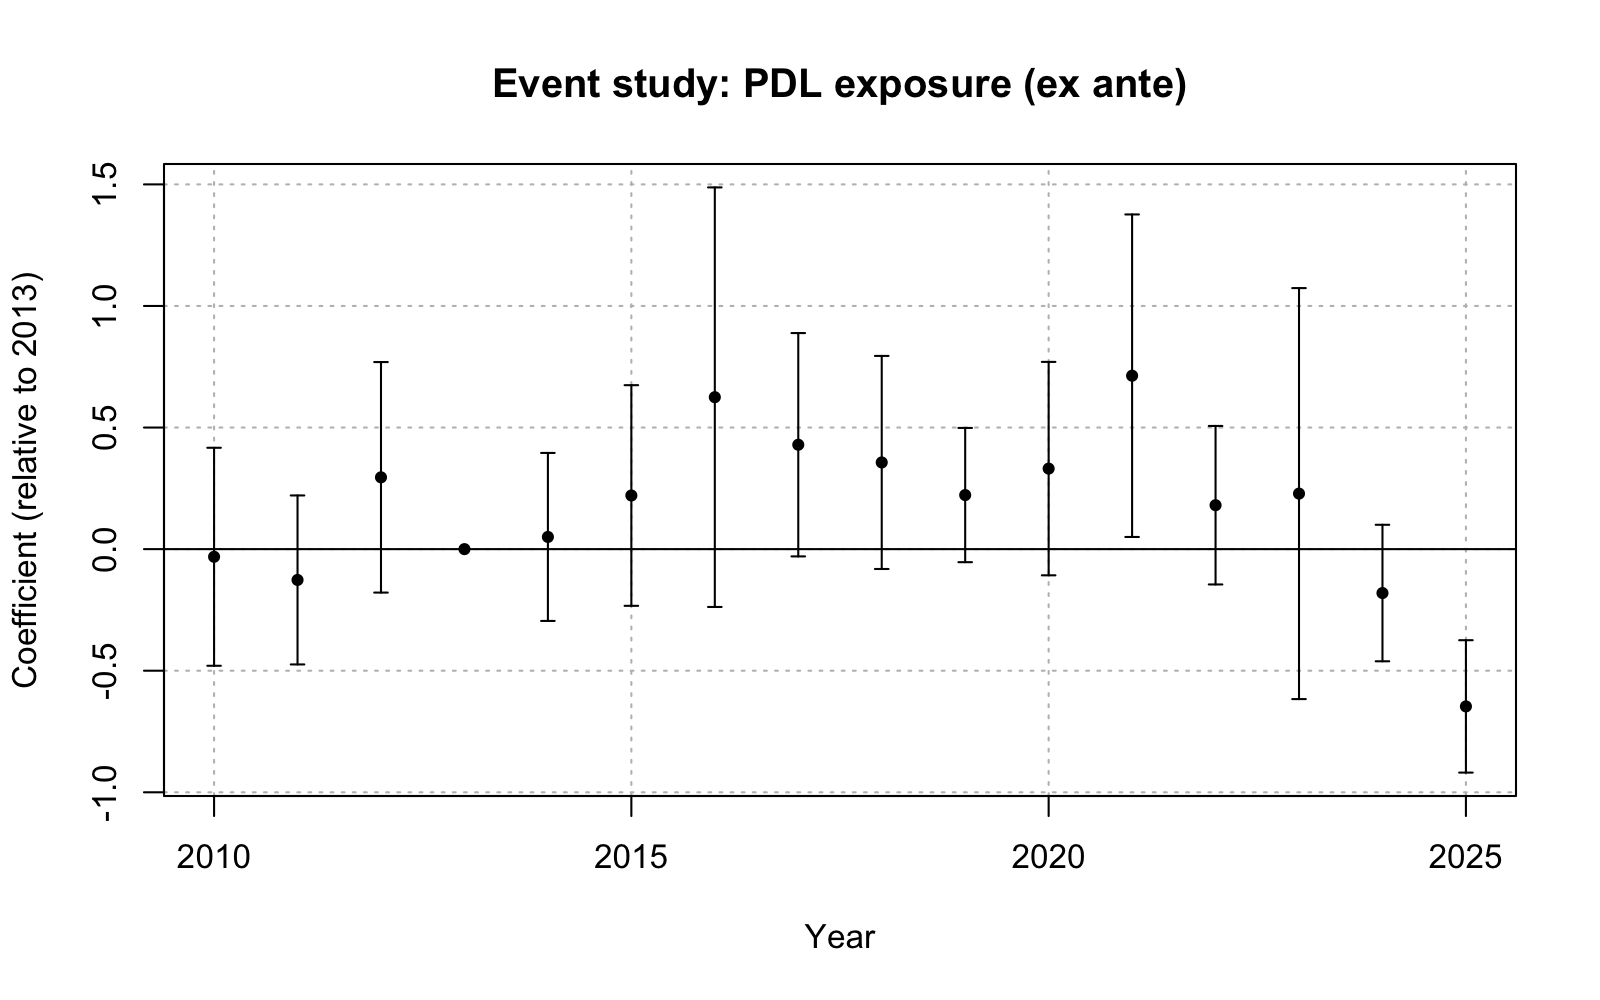
\includegraphics[width=\linewidth]{../output/RQ2/fda_feols_exante_pdl.png}
  \caption{FEOLS event study: FDA approvals, PDL exposure (ex-ante)}
  \label{fig:rq2_fda_feols_exante_pdl}
\end{figure}

\begin{figure}[!h]
  \centering
  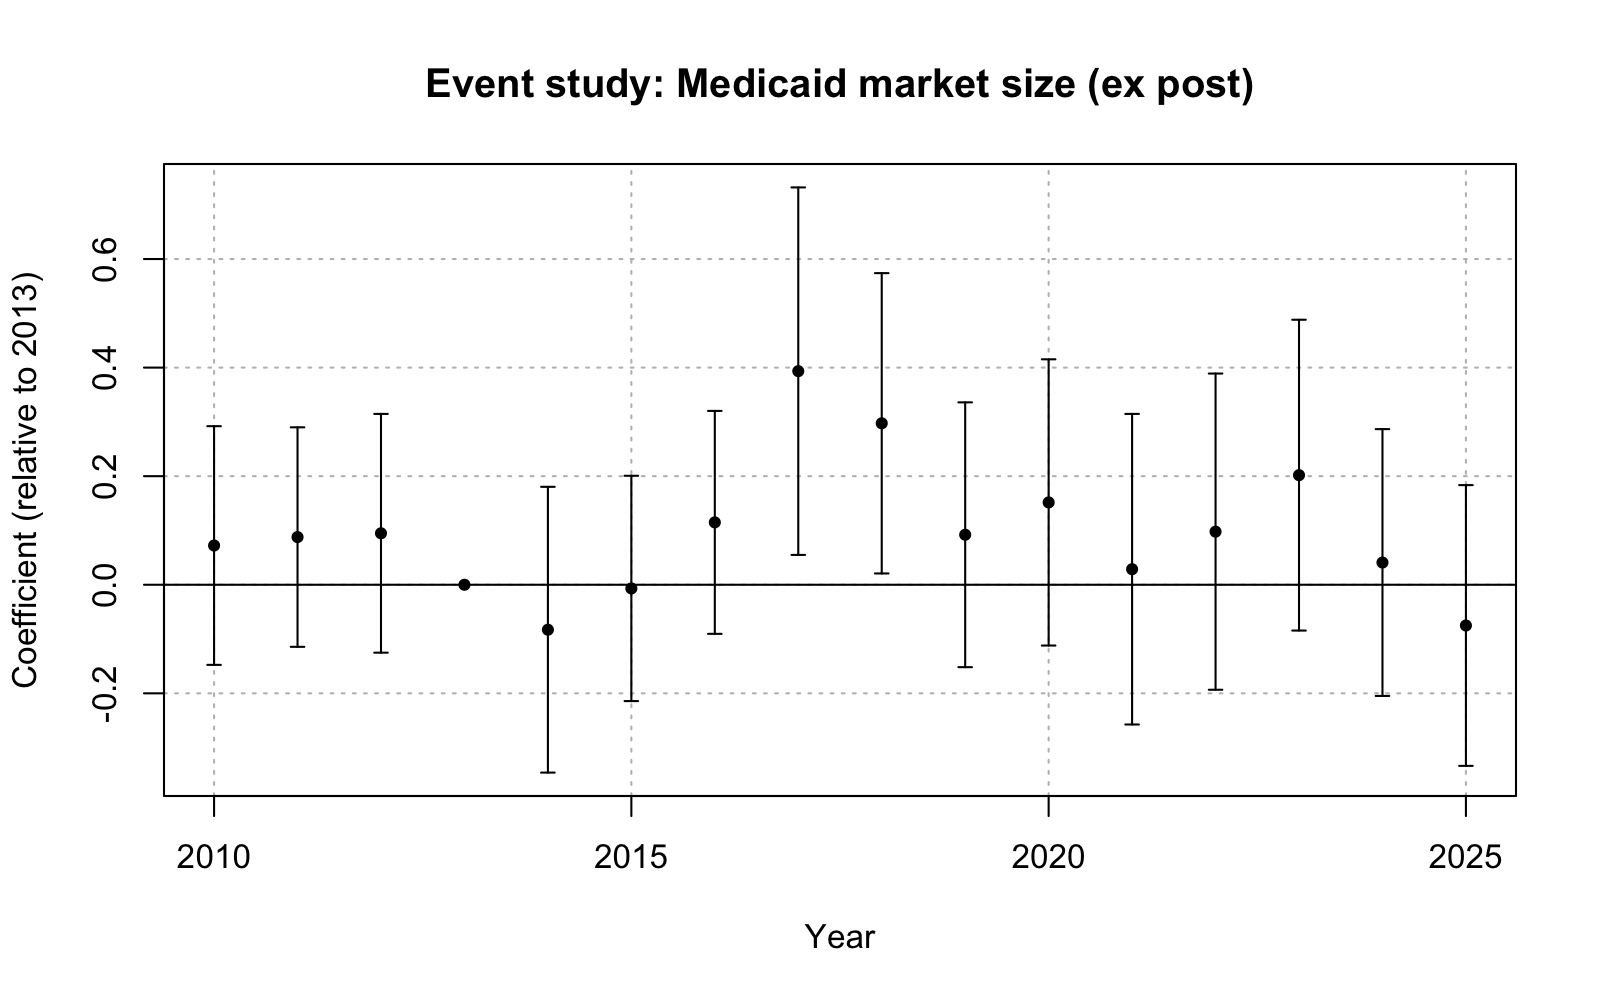
\includegraphics[width=\linewidth]{../output/RQ2/fda_feols_expost_medicaid.png}
  \caption{FEOLS event study: FDA approvals, Medicaid exposure (ex-post)}
  \label{fig:rq2_fda_feols_expost_medicaid}
\end{figure}

\begin{figure}[!h]
  \centering
  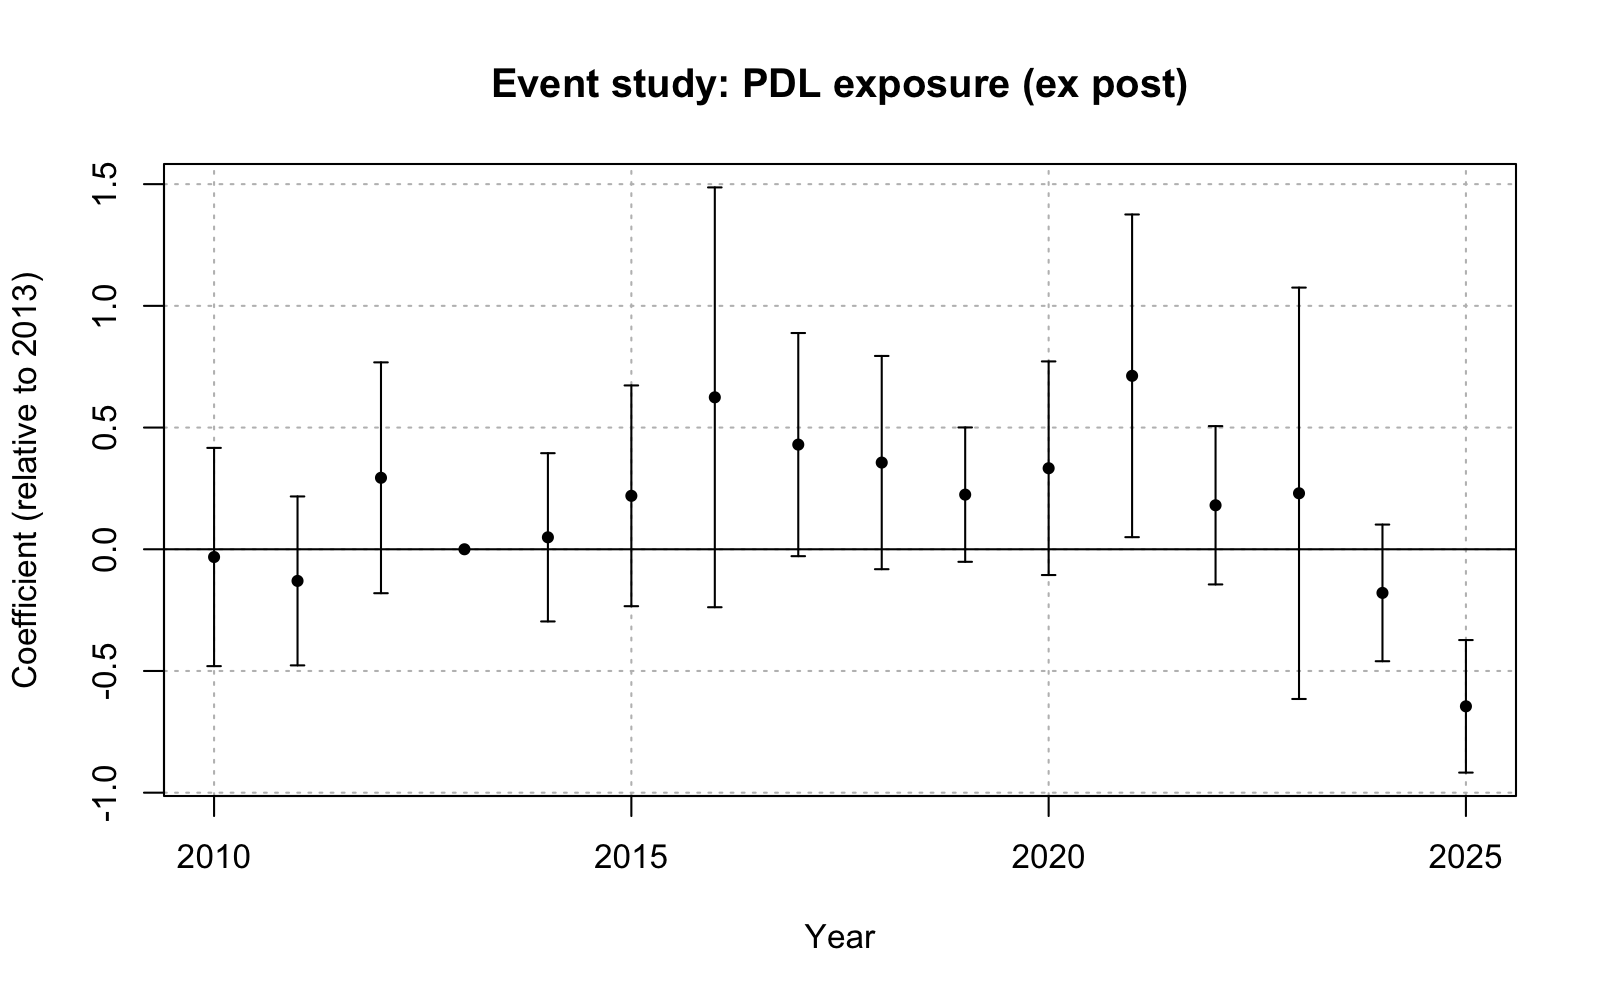
\includegraphics[width=\linewidth]{../output/RQ2/fda_feols_expost_pdl.png}
  \caption{FEOLS event study: FDA approvals, PDL exposure (ex-post)}
  \label{fig:rq2_fda_feols_expost_pdl}
\end{figure}

\clearpage
\begingroup\footnotesize
\begin{table}
\centering
\begin{talltblr}[         %% tabularray outer open
entry=none,label=none,
note{}={* p \num{< 0.05}, ** p \num{< 0.01}, *** p \num{< 0.001}},
]                     %% tabularray outer close
{                     %% tabularray inner open
width=\linewidth,
colspec={Q[]X[]X[]X[]X[]},
column{2,3,4,5}={}{halign=c,},
column{1}={}{halign=l,},
hline{33}={1,2,3,4,5}{solid, black, 0.05em},
}                     %% tabularray inner close
\toprule
& \SetCell[c=2]{c} FEOLS: Ex Ante && \SetCell[c=2]{c} FEOLS: Ex Post & \\
& Medicaid Share & PDL Exposure & Medicaid Share & PDL Exposure \\ \midrule
2010 & \num{0.214}   & \num{0.049}   & \num{0.285}   & \num{0.046}   \\
     & (\num{0.461}) & (\num{0.807}) & (\num{0.448}) & (\num{0.807}) \\
2011 & \num{-0.010}  & \num{-0.243}  & \num{0.344}   & \num{-0.257}  \\
     & (\num{0.382}) & (\num{0.712}) & (\num{0.412}) & (\num{0.711}) \\
2012 & \num{0.171}   & \num{1.402}   & \num{0.371}   & \num{1.395}   \\
     & (\num{0.406}) & (\num{0.911}) & (\num{0.447}) & (\num{0.912}) \\
2014 & \num{-0.333}  & \num{0.403}   & \num{-0.338}  & \num{0.398}   \\
     & (\num{0.465}) & (\num{0.647}) & (\num{0.536}) & (\num{0.647}) \\
2015 & \num{-0.088}  & \num{1.163}   & \num{-0.037}  & \num{1.158}   \\
     & (\num{0.478}) & (\num{0.881}) & (\num{0.422}) & (\num{0.881}) \\
2016 & \num{0.334}   & \num{2.645}   & \num{0.456}   & \num{2.642}   \\
     & (\num{0.426}) & (\num{1.683}) & (\num{0.418}) & (\num{1.682}) \\
2017 & \num{1.364}*  & \num{1.923}   & \num{1.566}*  & \num{1.924}   \\
     & (\num{0.680}) & (\num{0.994}) & (\num{0.690}) & (\num{0.992}) \\
2018 & \num{0.949}   & \num{1.684}   & \num{1.181}*  & \num{1.683}   \\
     & (\num{0.552}) & (\num{1.021}) & (\num{0.563}) & (\num{1.021}) \\
2019 & \num{0.519}   & \num{1.164}*  & \num{0.359}   & \num{1.171}*  \\
     & (\num{0.539}) & (\num{0.592}) & (\num{0.498}) & (\num{0.591}) \\
2020 & \num{0.687}   & \num{1.579}   & \num{0.598}   & \num{1.585}   \\
     & (\num{0.514}) & (\num{0.942}) & (\num{0.537}) & (\num{0.942}) \\
2021 & \num{0.038}   & \num{3.114}*  & \num{0.103}   & \num{3.110}*  \\
     & (\num{0.640}) & (\num{1.394}) & (\num{0.583}) & (\num{1.393}) \\
2022 & \num{0.333}   & \num{0.994}   & \num{0.381}   & \num{0.994}   \\
     & (\num{0.648}) & (\num{0.655}) & (\num{0.593}) & (\num{0.653}) \\
2023 & \num{0.809}   & \num{1.185}   & \num{0.798}   & \num{1.191}   \\
     & (\num{0.649}) & (\num{1.738}) & (\num{0.583}) & (\num{1.737}) \\
2024 & \num{0.272}   & \num{-0.452}  & \num{0.154}   & \num{-0.447}  \\
     & (\num{0.523}) & (\num{0.590}) & (\num{0.501}) & (\num{0.589}) \\
2025 & \num{-0.109}  & \num{-1.118}  & \num{-0.347}  & \num{-1.113}  \\
     & (\num{0.506}) & (\num{0.908}) & (\num{0.525}) & (\num{0.908}) \\
Num. obs. & \num{151200} & & \num{151200} & \\
R2        & \num{0.609}  & & \num{0.609}  & \\
\bottomrule
\end{talltblr}
\end{table}

\endgroup

\clearpage

% -----------------------------------------------------------------------
\section{RQ3: Therapeutic-Class Heterogeneity}
% -----------------------------------------------------------------------

\subsection{Patents}

\begin{center}
\begingroup\footnotesize
\begin{table}
\centering
\begin{talltblr}[         %% tabularray outer open
entry=none,label=none,
note{}={* p \num{< 0.05}, ** p \num{< 0.01}, *** p \num{< 0.001}},
]                     %% tabularray outer close
{                     %% tabularray inner open
colspec={Q[]Q[]Q[]},
column{2,3}={}{halign=c,},
column{1}={}{halign=l,},
hline{26}={1,2,3}{solid, black, 0.05em},
}                     %% tabularray inner close
\toprule
& FEOLS: Ex Ante & FEOLS: Ex Post \\ \midrule
Medicaid Share × ATC = A & \num{-0.165}*** & \num{-0.157}*** \\
& (\num{0.033})   & (\num{0.031})   \\
Medicaid Share × ATC = B & \num{0.134}***  & \num{0.151}***  \\
& (\num{0.024})   & (\num{0.027})   \\
Medicaid Share × ATC = C & \num{-0.123}*** & \num{-0.094}*** \\
& (\num{0.019})   & (\num{0.015})   \\
Medicaid Share × ATC = D & \num{-0.030}    & \num{-0.017}    \\
& (\num{0.108})   & (\num{0.062})   \\
Medicaid Share × ATC = G & \num{0.037}     & \num{0.032}     \\
& (\num{0.056})   & (\num{0.049})   \\
Medicaid Share × ATC = H & \num{0.876}***  & \num{0.619}***  \\
& (\num{0.136})   & (\num{0.096})   \\
Medicaid Share × ATC = J & \num{0.055}     & \num{0.035}     \\
& (\num{0.054})   & (\num{0.034})   \\
Medicaid Share × ATC = L & \num{0.346}     & \num{0.443}     \\
& (\num{0.452})   & (\num{0.578})   \\
Medicaid Share × ATC = M & \num{-0.336}*** & \num{-0.212}*** \\
& (\num{0.076})   & (\num{0.048})   \\
Medicaid Share × ATC = N & \num{-0.125}*** & \num{-0.174}*** \\
& (\num{0.028})   & (\num{0.039})   \\
Medicaid Share × ATC = R & \num{0.005}     & \num{0.005}     \\
& (\num{0.003})   & (\num{0.003})   \\
Medicaid Share × ATC = S & \num{0.093}***  & \num{0.105}***  \\
& (\num{0.017})   & (\num{0.020})   \\
Num. obs.                & \num{19617728}  & \num{19617728}  \\
R2                       & \num{0.247}     & \num{0.247}     \\
\bottomrule
\end{talltblr}
\end{table}

\endgroup
\end{center}

\subsection{FDA Approvals}

\begin{center}
\begingroup\footnotesize
\begin{table}
\centering
\begin{talltblr}[         %% tabularray outer open
entry=none,label=none,
note{}={* p \num{< 0.05}, ** p \num{< 0.01}, *** p \num{< 0.001}},
]                     %% tabularray outer close
{                     %% tabularray inner open
colspec={Q[]Q[]Q[]},
column{2,3}={}{halign=c,},
column{1}={}{halign=l,},
hline{26}={1,2,3}{solid, black, 0.05em},
}                     %% tabularray inner close
\toprule
& FEOLS: Ex Ante & FEOLS: Ex Post \\ \midrule %% TinyTableHeader
Medicaid Share × ATC = A & \num{1.211}** & \num{1.301}** \\
& (\num{0.391}) & (\num{0.420}) \\
Medicaid Share × ATC = B & \num{-0.396}  & \num{-0.121}  \\
& (\num{2.567}) & (\num{0.784}) \\
Medicaid Share × ATC = C & \num{0.229}   & \num{0.373}   \\
& (\num{0.171}) & (\num{0.278}) \\
Medicaid Share × ATC = D & \num{0.707}** & \num{0.881}** \\
& (\num{0.270}) & (\num{0.337}) \\
Medicaid Share × ATC = G & \num{-2.516}  & \num{-1.058}  \\
& (\num{2.666}) & (\num{1.121}) \\
Medicaid Share × ATC = H & \num{1.144}   & \num{0.446}   \\
& (\num{1.358}) & (\num{0.530}) \\
Medicaid Share × ATC = J & \num{-0.145}  & \num{-0.078}  \\
& (\num{0.165}) & (\num{0.089}) \\
Medicaid Share × ATC = L & \num{-0.321}  & \num{-0.244}  \\
& (\num{2.789}) & (\num{2.115}) \\
Medicaid Share × ATC = M & \num{0.022}   & \num{0.017}   \\
& (\num{1.127}) & (\num{0.858}) \\
Medicaid Share × ATC = N & \num{0.034}   & \num{0.047}   \\
& (\num{0.074}) & (\num{0.101}) \\
Medicaid Share × ATC = R & \num{0.298}   & \num{0.178}   \\
& (\num{0.217}) & (\num{0.130}) \\
Medicaid Share × ATC = S & \num{8.052}*  & \num{6.473}*  \\
& (\num{3.737}) & (\num{3.004}) \\
Num. obs.                                           & \num{561600}  & \num{561600}  \\
R2                                                  & \num{0.235}   & \num{0.235}   \\
\bottomrule
\end{talltblr}
\end{table}

\endgroup
\end{center}

\clearpage

% -----------------------------------------------------------------------
\section{PDL Counterfactual Analysis}
% -----------------------------------------------------------------------

\begin{center}
\begingroup\footnotesize
\begin{table}
\centering
\begin{talltblr}[         %% tabularray outer open
entry=none,label=none,
note{}={* p \num{< 0.05}, ** p \num{< 0.01}, *** p \num{< 0.001}},
]                     %% tabularray outer close
{                     %% tabularray inner open
width=\linewidth,
colspec={Q[]X[]X[]},
column{2,3}={}{halign=c,},
column{1}={}{halign=l,},
hline{8}={1,2,3}{solid, black, 0.05em},
}                     %% tabularray inner close
\toprule
& Patents & FDA Approvals \\ \midrule %% TinyTableHeader
Post $\times$ P\&T Pass & \num{-11.399}*  & \num{1.002}   \\
& (\num{4.663})   & (\num{0.633}) \\
Post $\times$ Price Pass & \num{-7.386}*** & \num{0.057}   \\
& (\num{2.173})   & (\num{0.881}) \\
Post $\times$ In PDL & \num{15.549}**  & \num{-0.112}  \\
& (\num{5.215})   & (\num{1.174}) \\
Num. obs.                                 & \num{5281696}   & \num{151200}  \\
R2                                        & \num{0.535}     & \num{0.609}   \\
\bottomrule
\end{talltblr}
\end{table}

\endgroup
\end{center}

\clearpage

\bibliographystyle{apalike}
\bibliography{references}

\end{document}

\documentclass[12pt]{article}
\usepackage{geometry}
\geometry{a4paper, portrait, margin=1in}

% --- Math Packages ---
\usepackage{amsmath}
\usepackage{amssymb}
\usepackage{amsfonts}
\usepackage{amsthm}

% --- Graphics & Diagrams ---
\usepackage{graphicx}
\usepackage{tikz}
\usetikzlibrary{shapes, arrows, positioning}

% --- Formatting ---
\usepackage{parskip}
\usepackage[hidelinks]{hyperref}
\usepackage{natbib}
\usepackage{enumitem}
\usepackage{booktabs}
\usepackage{caption}
\usepackage{float}
\usepackage{siunitx}
\usepackage{tabularray}
\UseTblrLibrary{booktabs, siunitx}
\pagestyle{plain}

% --- Allow talltblr to break across pages ---
\renewenvironment{table}[1][]{}{}

% --- Word count (requires compiling with --shell-escape) ---
\newcommand{\wordcount}{%
  \immediate\write18{texcount -sum -1 \jobname.tex 2>/dev/null | python3 -c "import sys; n=sys.stdin.read().strip(); print(f'{int(n):,}') if n.isdigit() else print('?')" > \jobname.wc}%
  \input{\jobname.wc}%
}

\title{MPhil Thesis: Robustness and Sensitivity Analysis}
\author{Mohammad-Shah Karim}
\date{May 2026}

\begin{document}

\maketitle

\begin{center}
  \small Word count: \wordcount
\end{center}

\tableofcontents

\newpage

% -----------------------------------------------------------------------
\section{Robustness and Sensitivity Analysis}
% -----------------------------------------------------------------------

The baseline results are estimated using FEOLS with an ex-ante Medicaid market share measure as a proxy for firm-class exposure to the Medicaid reform. This section examines the sensitivity of these findings to alternative specifications, estimation methods, and treatment of the continuous exposure variable. Each research question is addressed in turn.

% -----------------------------------------------------------------------
\subsection{RQ1: Overall Innovation Response}
% -----------------------------------------------------------------------

\subsubsection{Ex-Post Medicaid Exposure}

The baseline specification uses pre-expansion Medicaid market shares to measure treatment intensity. Ex-post market shares are constructed from realised the Medicaid prescription shares in 2014-2015 as an alternative measure of exposure to the ACA. The window for ex-post shares is restricted to the first two years of the reform in order to capture initial shifts in demand without extending into periods where endogenous response in firm entry or prescribing behaviour, may contaminate the exposure measure. Estimates using ex-post exposure act purely as a robustness check since the measure would still reflect the actual post-expansion demand environment as opposed to being a predetermined exposure measure.

Under the estimated ex-post measure, the patent coefficients are nearly identical to the ex-ante estimates. The pre-expansion coefficients remain small and insignificant, highlighting robustness to the parallel trends assumption while the post-reform coefficients follow the same gradual negative trajectory, growing from $-0.088$ in 2015 to $-0.250$ by 2024 before dropping slightly to $-0.212$ in 2025. These estimates are consistent with the ex-ante result, which also has a 2024 peak at $-0.252$. Similarly, the coefficients for FDA approvals are also in line with the baseline specification, where the coefficients are largely statistically insignificant with the exception of 2017 and 2019, while having no clear directional pattern. The alignment between the ex-ante and ex-post results therefore indicates that the findings are orthogonal to the choice of exposure measure.

\begin{figure}[!h]
  \centering
  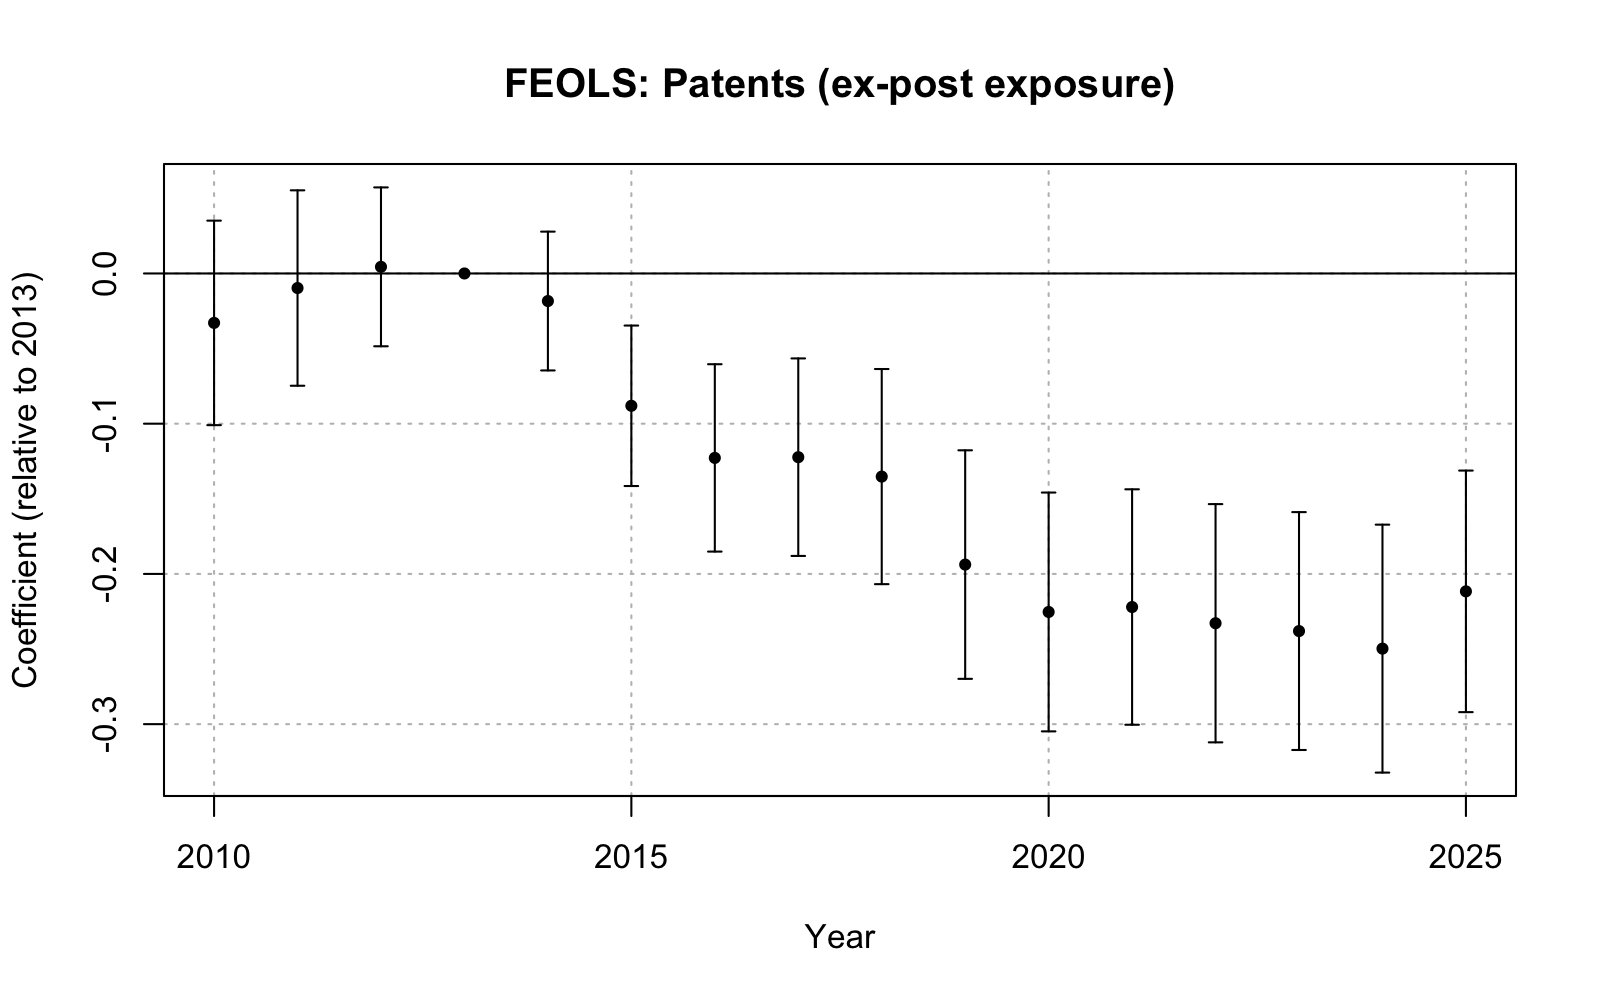
\includegraphics[width=\linewidth]{../output/RQ1/patent_feols_expost.png}
  \caption{FEOLS event study: patents, ex-post Medicaid exposure}
  \label{fig:rob_rq1_patent_feols_expost}
\end{figure}

\begin{figure}[!h]
  \centering
  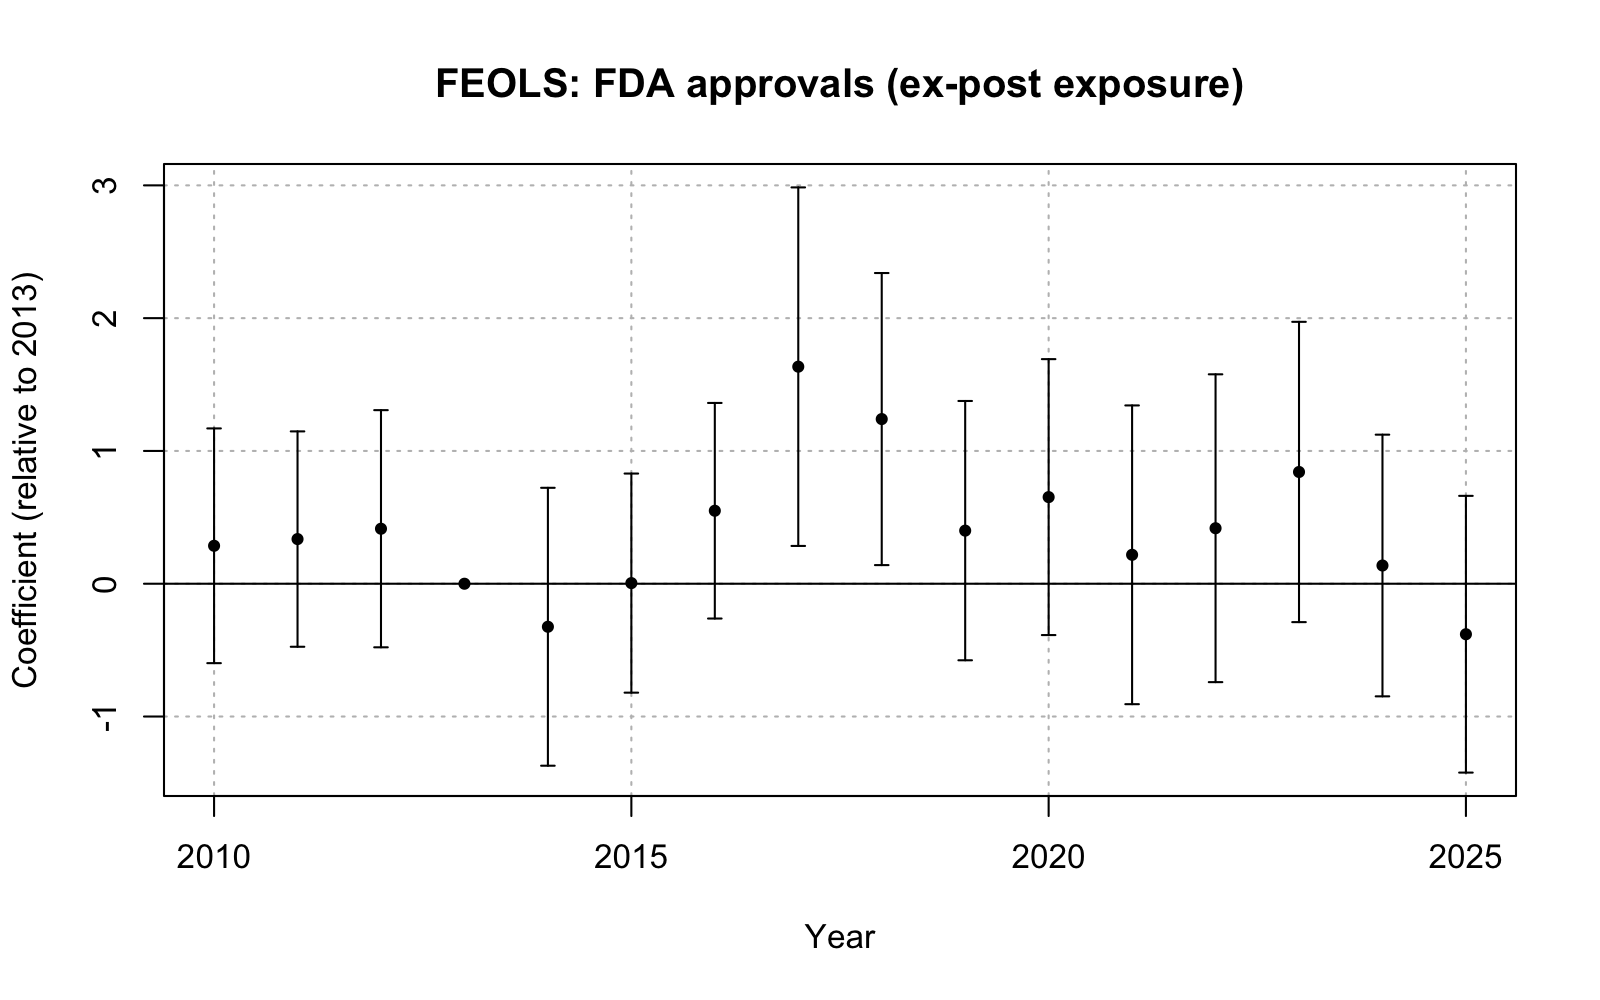
\includegraphics[width=\linewidth]{../output/RQ1/fda_feols_expost.png}
  \caption{FEOLS event study: FDA approvals, ex-post Medicaid exposure}
  \label{fig:rob_rq1_fda_feols_expost}
\end{figure}

\clearpage

\subsubsection{FE Poisson Estimation}

The baseline FEOLS specification models patent counts and FDA approvals linearly, although both outcomes are non-negative integer variables with substantial counts of zero. Consequently, the specification is re-estimated using a fixed-effects Poisson model, which therefore models the conditional mean of each of the innovation outcomes non-linearly. This allows for a robustness check on whether the baseline findings are sensitive to the linear treatment of the count outcomes, since the Poisson estimator remains consistent even when the outcome is overdispersed provided the conditional mean is correctly specified \citep{wooldridge1999distribution}.

The FE Poisson estimates for patents are consistent with the FEOLS results. Under the ex-ante specification, the pre-expansion coefficients are small and insignificant, providing support for the parallel trends assumption. The post-expansion coefficients are negative and grow in magnitude over time, peaking at $-1.474$ by 2024 and fall slightly in 2025, consistent with the FEOLS findings. Therefore, at its peak in 2024, a ten percentage point increase in Medicaid exposure corresponds to an approximate 14.7 percent decrease in patents on average. The ex-post FE Poisson estimates follow a similar trajectory, with the 2024 peak being more negative at $-2.021$.

While the FDA approval estimates under the Poisson model are uniformly negative, they still remain insignificant across both the ex-ante and ex-post specifications. This is a slight deviation from the baseline OLS results, where the FDA estimates fluctuate in sign, but both specifications agree that the innovation response at the approval stage remains statistically significant. The findings for both innovation outcomes are consistent between the linear and Poisson specifications, suggesting that the post-expansion patterns are not sensitive to modelling the count outcomes linearly.

\begin{figure}[!h]
  \centering
  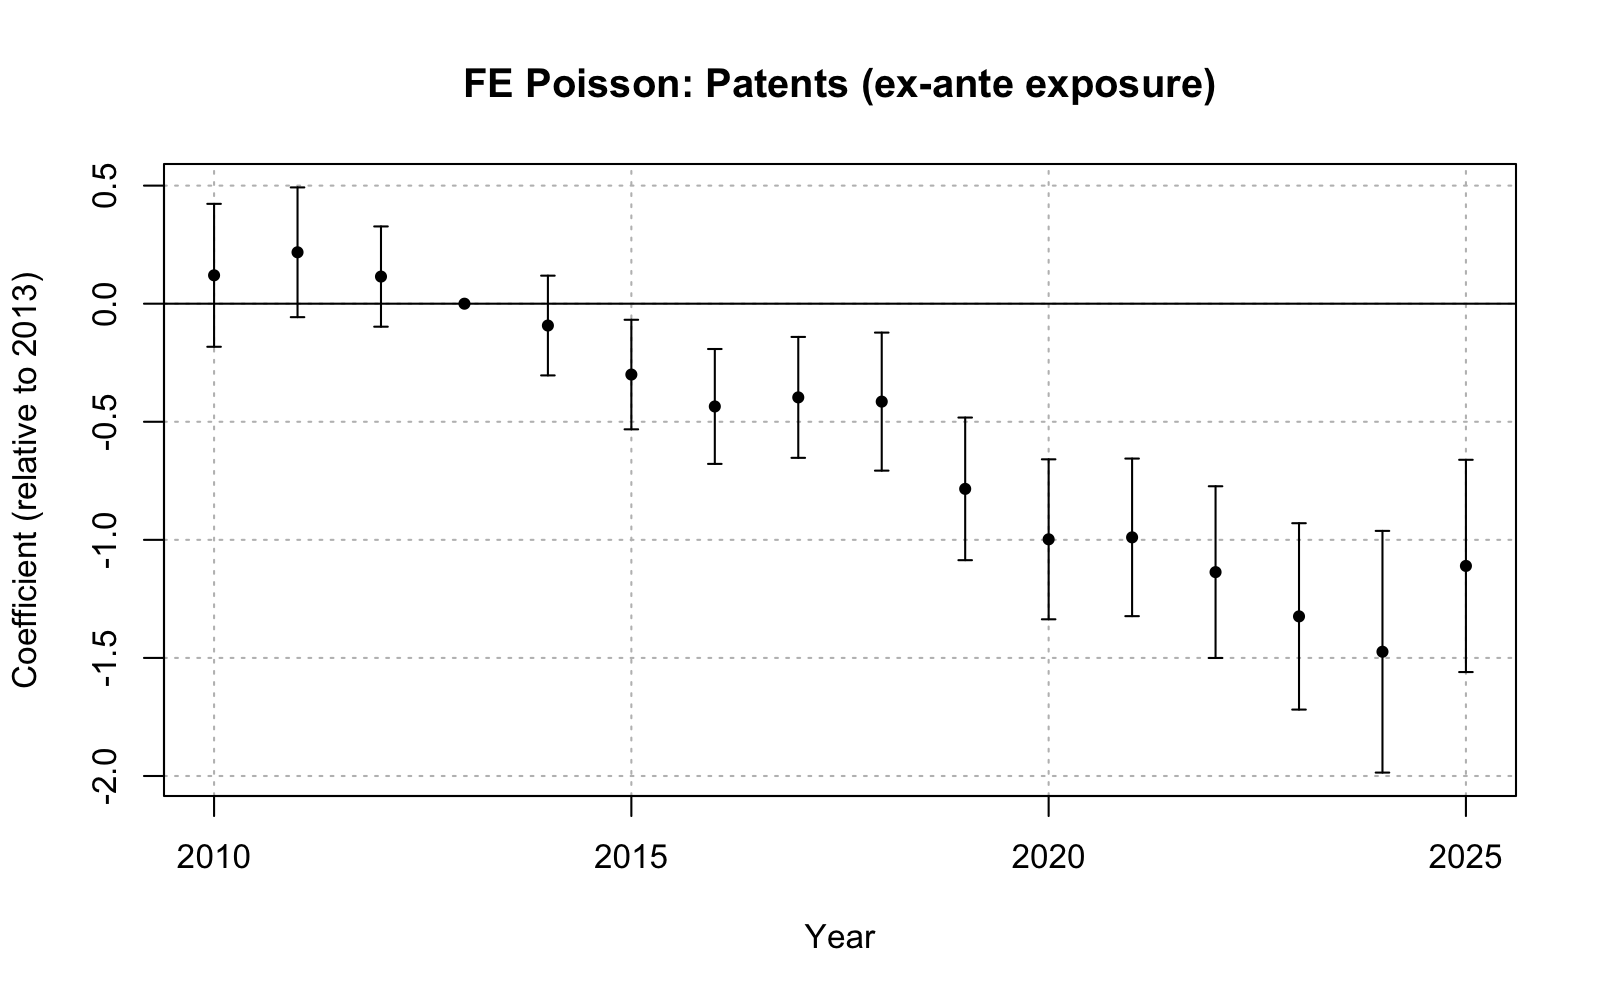
\includegraphics[width=\linewidth]{../output/RQ1/patent_poi_exante.png}
  \caption{FE Poisson event study: patents, ex-ante Medicaid exposure}
  \label{fig:rob_rq1_patent_poi_exante}
\end{figure}

\begin{figure}[!h]
  \centering
  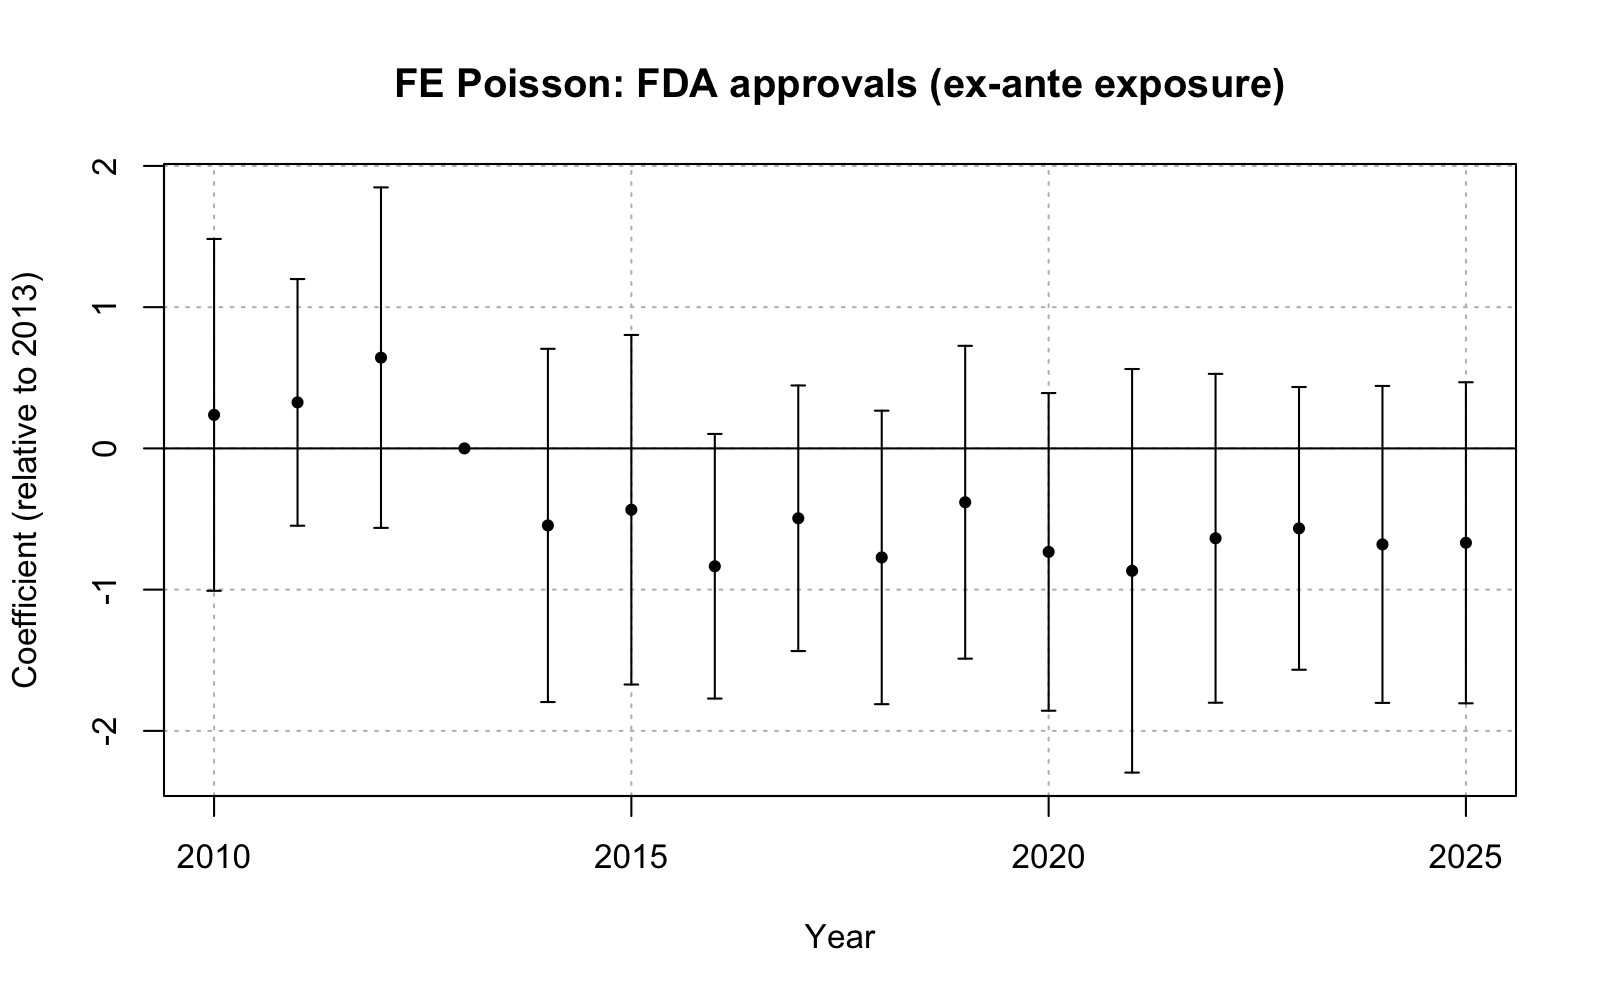
\includegraphics[width=\linewidth]{../output/RQ1/fda_poi_exante.png}
  \caption{FE Poisson event study: FDA approvals, ex-ante Medicaid exposure}
  \label{fig:rob_rq1_fda_poi_exante}
\end{figure}

\clearpage

\subsubsection{Binned Treatment Intensity}

The baseline specification treats exposure to the ACA as a continuous variable. As an alternative test, therapeutic classes are grouped into low, medium and high exposure bins, allowing for separate event-study coefficients to be estimated across different parts of the Medicaid exposure distribution. This relaxes the assumption of linearity in treatment effects imposed by the continuous specification, and examines whether the post-expansion response is concentrated among classes which are greater exposed to the Medicaid reform.

Therapeutic classes are grouped into the three bins based on their ex-ante Medicaid market shares, as reported in Table~\ref{tab:atc_bins}. Nervous system and cardiovascular drugs form the high-exposure bin, as their Medicaid market shares are substantially larger than other class shares. An approximate threshold of 10\% is used to distinguish between the medium and low bin classes, thus anti-infectives and dermatologicals form the medium-exposure bin.


\begingroup
\makeatletter
\renewenvironment{table}[1][tbp]{\@float{table}[#1]}{\end@float}
\makeatother
\begin{table}[htbp]
\centering
\caption{Pre-expansion Medicaid market shares and bin assignments}
\label{tab:atc_bins}
\begin{tabular}{llrl}
\toprule
\multicolumn{1}{c}{ATC} & \multicolumn{1}{c}{Therapeutic Area} & \multicolumn{1}{c}{Medicaid Share} & \multicolumn{1}{c}{Bin} \\
\midrule
N & Nervous system                  & 0.363 & High   \\
C & Cardiovascular system           & 0.215 & High   \\
J & Anti-infectives for systemic use & 0.120 & Medium \\
D & Dermatologicals                 & 0.099 & Medium \\
R & Respiratory system              & 0.085 & Low    \\
A & Alimentary tract and metabolism & 0.068 & Low    \\
M & Musculo-skeletal system         & 0.015 & Low    \\
H & Systemic hormonal preparations  & 0.012 & Low    \\
L & Antineoplastic and immunomodulating agents & 0.006 & Low \\
G & Genito-urinary system and sex hormones     & 0.006 & Low \\
S & Sensory organs                  & 0.005 & Low    \\
B & Blood and blood-forming organs  & 0.005 & Low    \\
V & Various                         & 0.000 & Low    \\
P & Antiparasitic products          & 0.000 & Low    \\
\bottomrule
\end{tabular}
\end{table}

\endgroup

The low exposure bin is omitted from the regression, so the coefficients for the high and medium bins are estimated relative to the low-exposure bin. The pre-expansion coefficients for both the high and medium-exposure patent bins are small and statistically insignificant, supporting the parallel trends assumption within each group. While the medium-exposure bin largely contain positive insignificant coefficients throughout the post-expansion period with a peak decline of $-0.02$ in 2025, the high-exposure bin exhibit a growing negative trajectory with coefficients reaching $-0.155$ by the same year. This reinforces the finding from RQ3 that the post-expansion patenting decline driven by classes at the upper end of the Medicaid exposure distribution. Importantly, the relative magnitude of the high and medium exposure coefficients is disproportionately larger than their respective Medicaid market shares. On average, exposure of the high bin is approximately $2.5$ times larger than the medium bin, yet the peak patent responses approximately differ by a factor of eight. This suggests that the relationship between Medicaid exposure and patenting may be convex, with the response intensifying at greater levels of exposure as opposed to scaling proportionally.

FDA approval estimates are statistically insignificant for both the high and medium-exposure bins throughout the sample period, and the pre-expansion coefficients are close to zero in both bins, supporting the parallel trends assumption. The absence of significant post-expansion effects for FDA approvals is consistent with the baseline findings and reinforces the interpretation that the innovation response has not yet propagated to the downstream approval stage. Unlike the patent results, the estimates from the FDA binned specification provide no evidence of a non-linear treatment effects across the Medicaid market share distribution, but this is driven by the absence of a detectable effect within each of the exposure bins rather than providing support for a linear relationship.

\clearpage

\begin{figure}[!h]
  \centering
  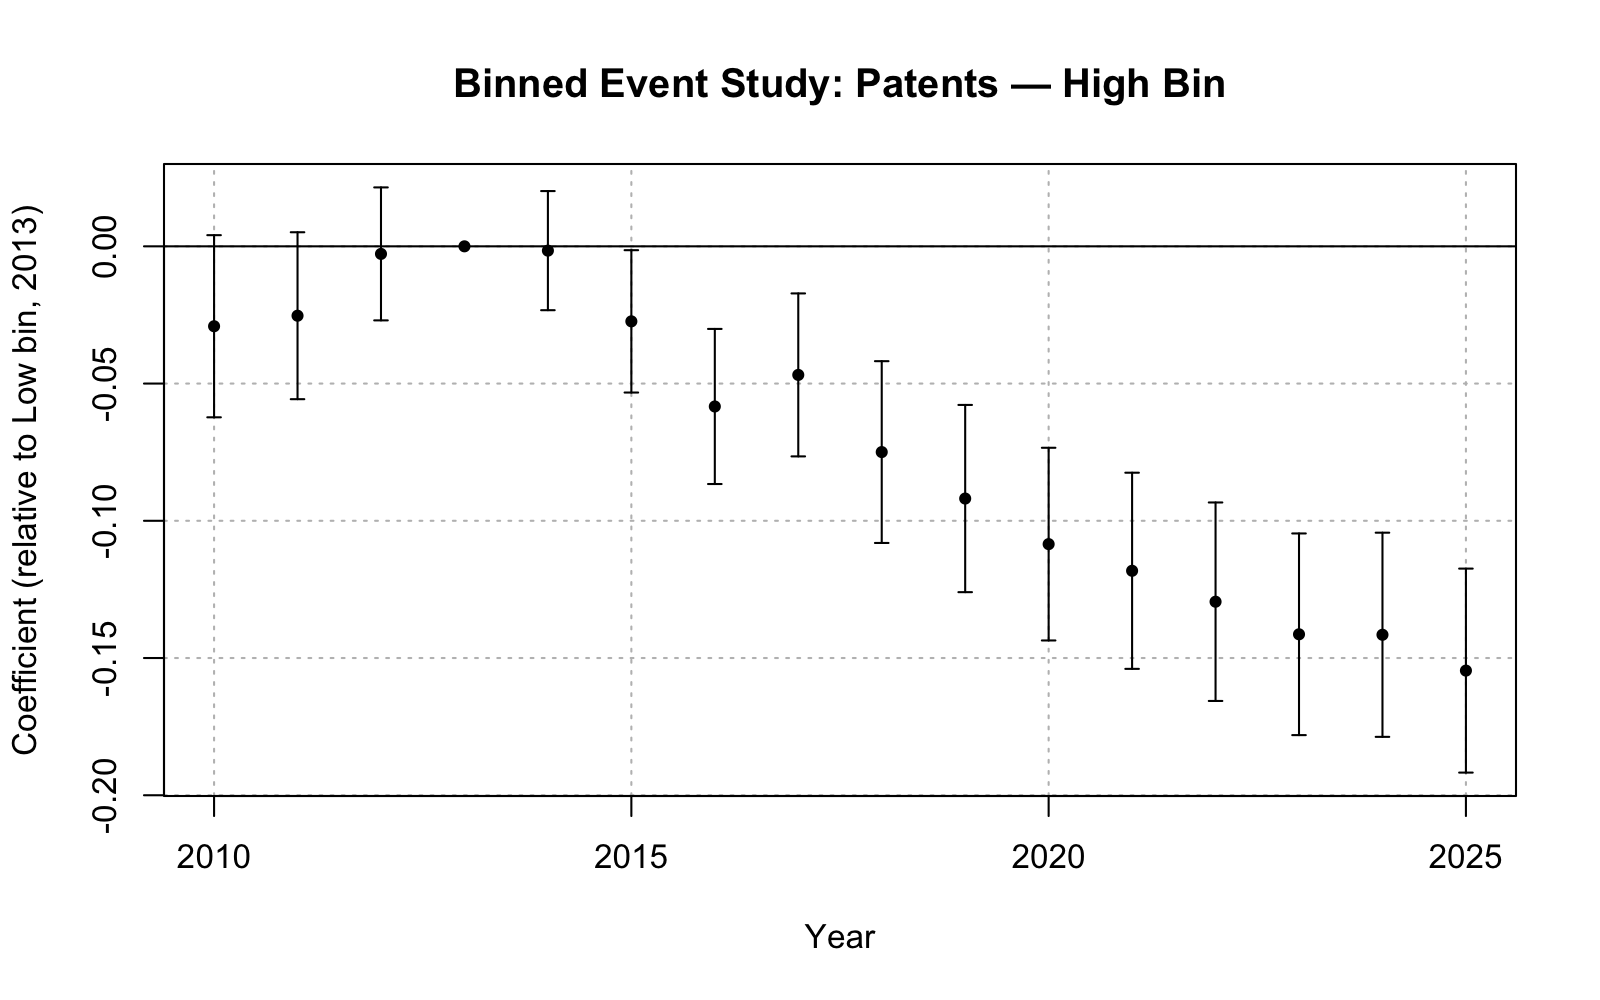
\includegraphics[width=\linewidth]{../output/robustness/binned_treatment/binned_patent_high_es.png}
  \caption{Binned event study: patents, high-exposure bin (N, C)}
  \label{fig:rob_binned_patent_high}
\end{figure}

\begin{figure}[!h]
  \centering
  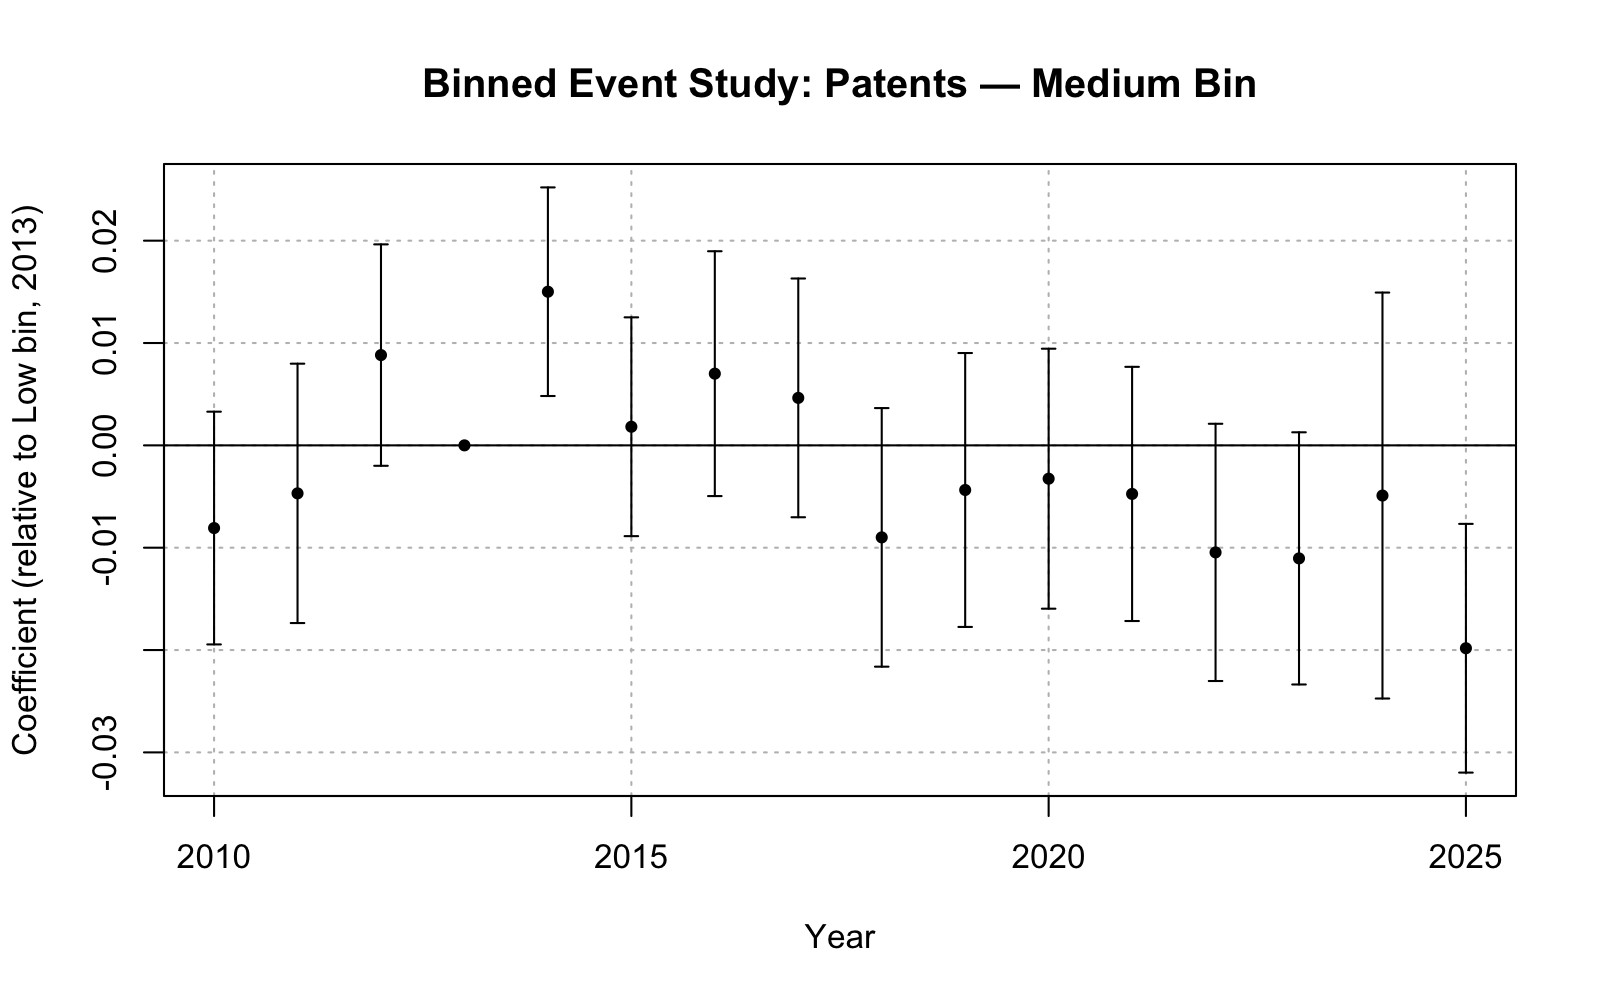
\includegraphics[width=\linewidth]{../output/robustness/binned_treatment/binned_patent_medium_es.png}
  \caption{Binned event study: patents, medium-exposure bin (J, D)}
  \label{fig:rob_binned_patent_medium}
\end{figure}

\clearpage

\begin{figure}[!h]
  \centering
  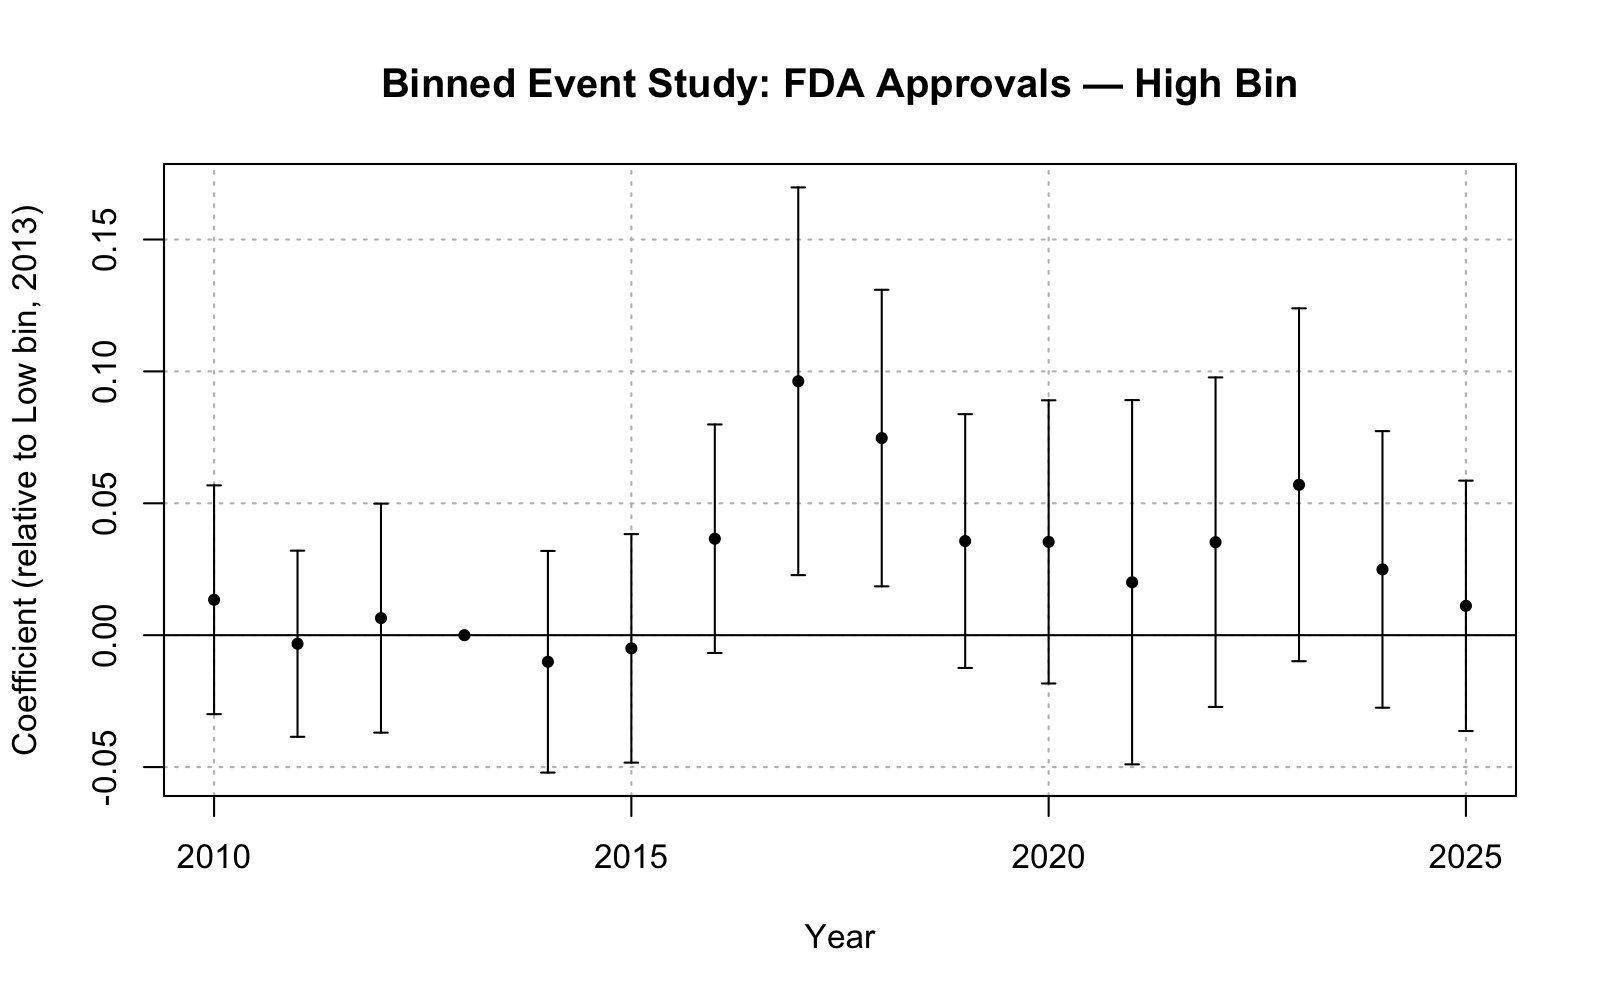
\includegraphics[width=\linewidth]{../output/robustness/binned_treatment/binned_fda_high_es.png}
  \caption{Binned event study: FDA approvals, high-exposure bin (N, C)}
  \label{fig:rob_binned_fda_high}
\end{figure}

\begin{figure}[!h]
  \centering
  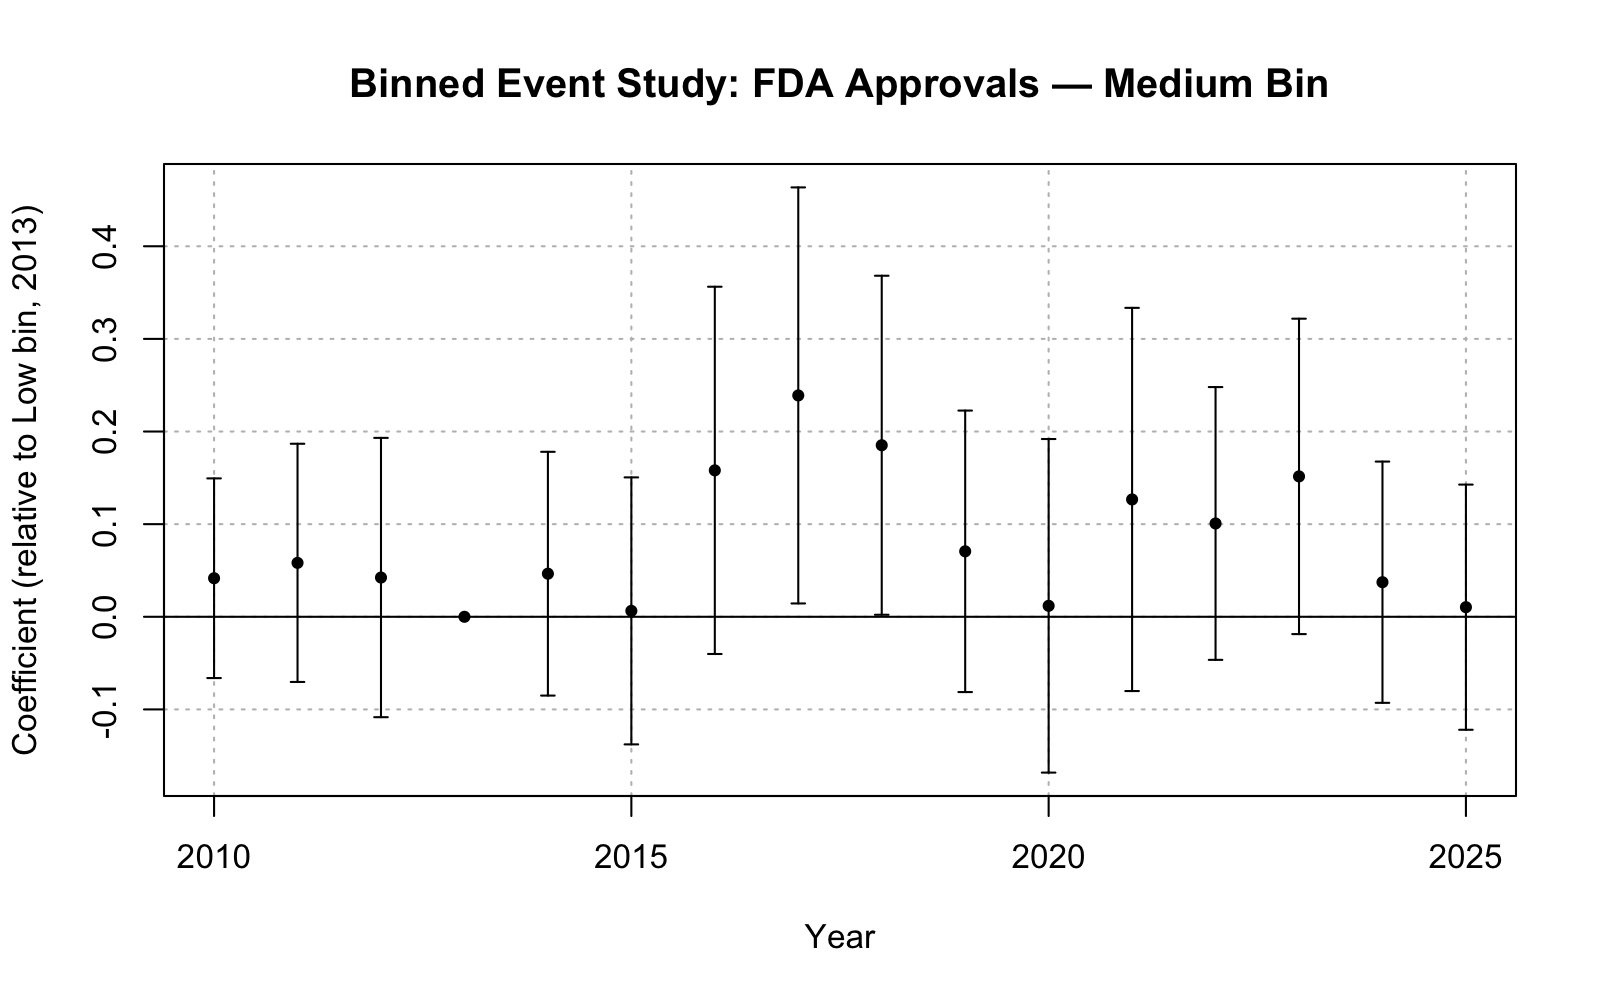
\includegraphics[width=\linewidth]{../output/robustness/binned_treatment/binned_fda_medium_es.png}
  \caption{Binned event study: FDA approvals, medium-exposure bin (J, D)}
  \label{fig:rob_binned_fda_medium}
\end{figure}

\clearpage

\subsubsection{Continuous Difference-in-Differences}

The binned event-study specification allowed for treatment effects to vary across the discrete groups, but the results were contingent on the boundaries specified for each exposure bin. Given this, the continuous difference-in-differences (Continuous DiD) estimator proposed by \citet{NBERw32117} is applied using the \texttt{contdid} R package \citep{contdid2025}. This estimator non-parametrically identifies dose-specific treatment effects at each exposure-level under the parallel trends assumption, thereby avoiding the need to discretise the treatment variable. Conventional TWFE estimators with continuous treatment can be difficult to interpret when treatment effects differ across the distribution of exposure level. The Continuous DiD estimator avoids this by aggregating the dose-specific estimates into event-study coefficients and assesses for pre-trends and post-treatment dynamics. The full set of coefficient estimates is reported in Table~\ref{tab:contdid_es}.

The Continuous DiD estimates for patents are consistent with the baseline results. The pre-expansion coefficients are small and statistically insignificant, supporting the parallel trends assumption. Notably, the coefficients are persistently significant from 2019 onwards, which is four years later than the 2015 onset under the baseline FEOLS model. This implies that the innovation response was not immediate as suggested by the baseline results, instead firms required several years to fully adjust their R\&D decisions in response to the expansion.

The FDA approval estimates under the Continuous DiD model are statistically insignificant throughout the entire period. The pre-period estimates are small and fluctuate around zero, while the post-expansion estimates are mostly positive. The absence of a clear FDA approval response to the Medicaid reform is therefore robust to modelling Medicaid exposure non-parametrically within the Continuous DiD framework.

Taken together, the results from the sensitivity analysis show that the main findings are robust to discretising market shares into exposure bins and using a non-parametric continuous DiD approach. Crucially, the sustained negative patent response remains visible under an estimator developed specifically for continuous-treatment DiD designs, while drug approvals do not appear to have a clear response to the ACA. The Continuous DiD estimates are also consistent with the binned analysis for highly exposed patents, while bins with medium exposure do not display a statistically significant response. This pattern is consistent with the class-level heterogeneity identified in RQ3, where nervous system and cardiovascular drugs were among the classes experiencing the greatest patent reductions.

\clearpage

\begin{figure}[!h]
  \centering
  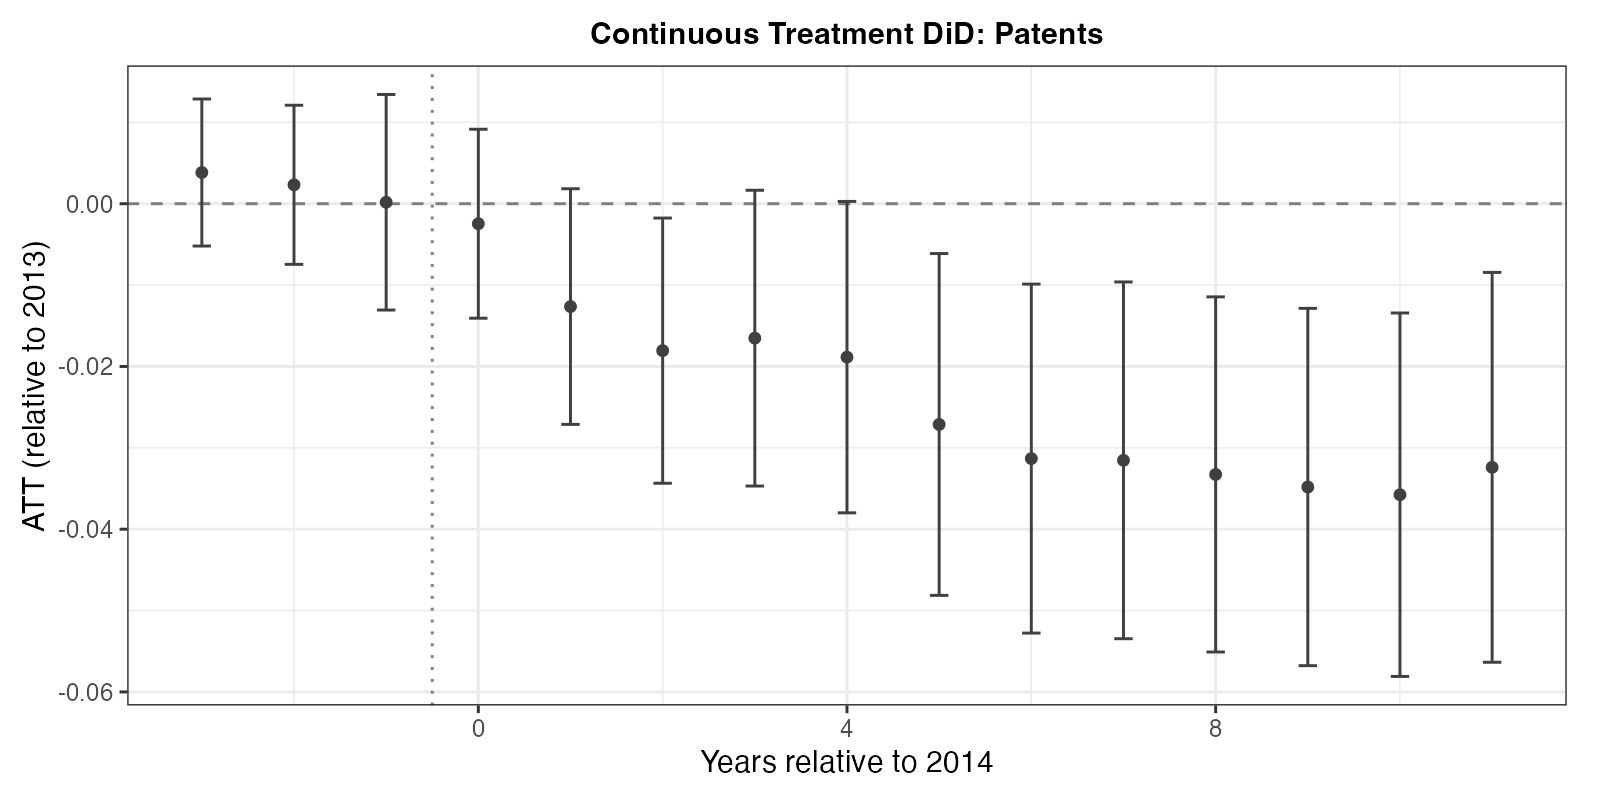
\includegraphics[width=\linewidth]{../output/robustness/contdid/contdid_patent_es.png}
  \caption{Continuous DiD event study: patents}
  \label{fig:rob_contdid_patent}
\end{figure}

\begin{figure}[!h]
  \centering
  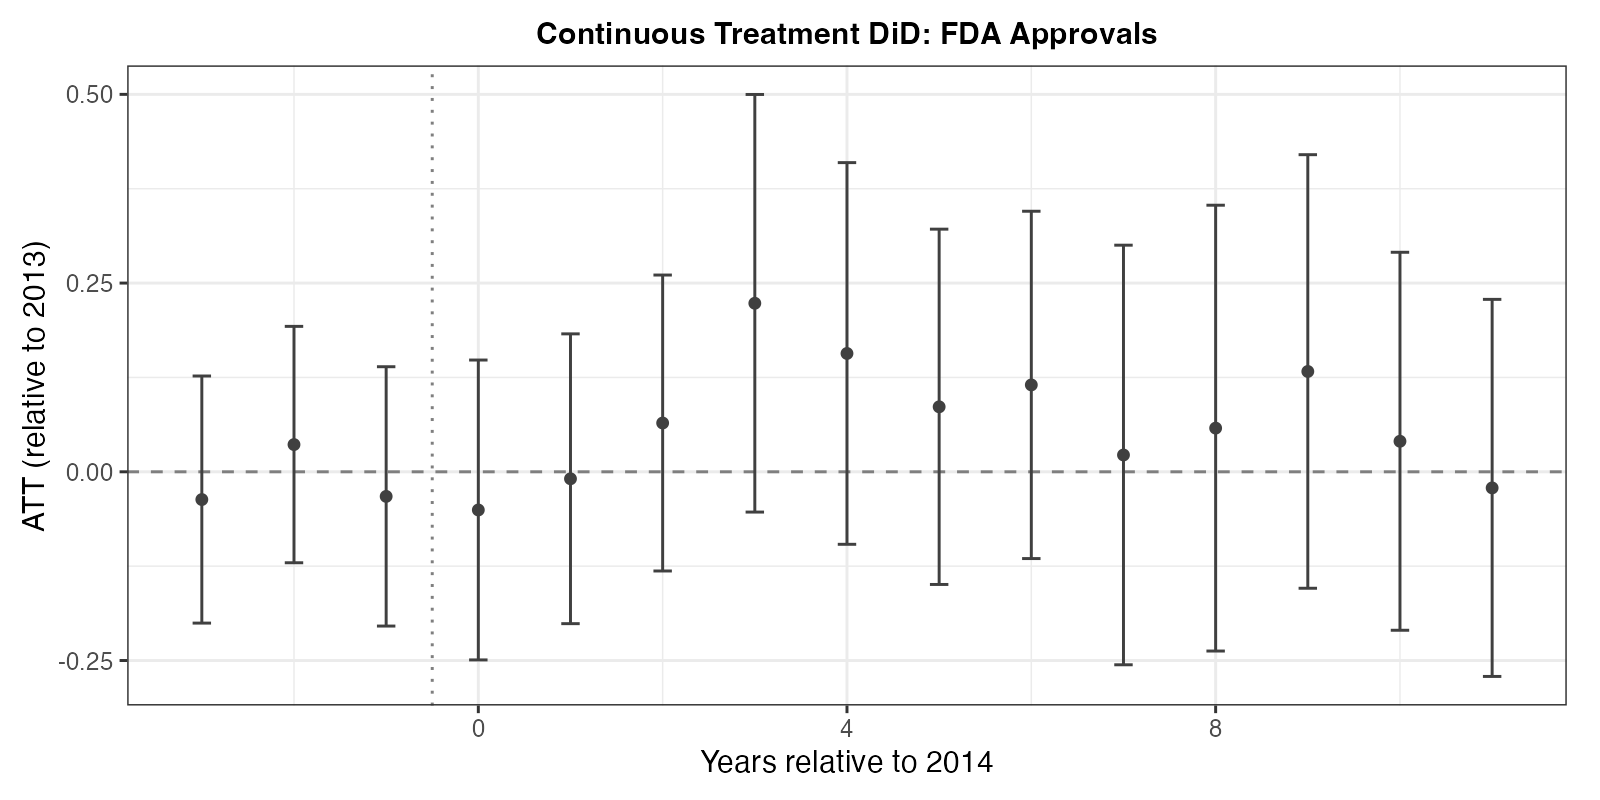
\includegraphics[width=\linewidth]{../output/robustness/contdid/contdid_fda_es.png}
  \caption{Continuous DiD event study: FDA approvals}
  \label{fig:rob_contdid_fda}
\end{figure}

\clearpage

% -----------------------------------------------------------------------
\subsection{RQ2: Medicaid Demand and PDL Exposure}
% -----------------------------------------------------------------------

\subsubsection{Ex-Post Medicaid Exposure}

The second specification jointly estimates the innovation response to Medicaid demand exposure and exposure to the PDL. Like RQ1, an ex-post market share measure is used to determine whether the estimates are sensitive to the construction of the exposure variable.

Once again, the ex-post Medicaid exposure coefficients for patents are nearly identical to the baseline results. The same reductions in Medicaid market share coefficients is observed, with the PDL exposure coefficient path also coinciding with the ex-ante model which saw negative coefficients from 2016 with significance from 2019. The pre-expansion coefficients for both the Medicaid and PDL measures remain small and statistically insignificant, supporting the parallel trends assumption even under the ex-post exposure construction.

The FDA approval coefficients are largely under the ex-post specification are statistically insignificant for both the Medicaid and PDL exposure measures, with isolated incidences of significance in a small number of post-expansion years. This aligns with the baseline finding that the innovation response has not yet reached the final stage of the R\&D pipeline. The agreement between the ex-ante and ex-post results therefore indicates that the decomposition into Medicaid demand and PDL exposure is not sensitive to the construction of exposure to Medicaid.

The FE Poisson, binned treatment, and continuous difference-in-differences estimators are not applied to the RQ2 specification. The joint estimation of two exposure variables under these alternative specifications is computationally demanding, and could not be completed with the device used for this study. Given this constraint, the alternative estimators are only used for the RQ1 specification where they are most informative for the aggregate response to the policy.

\clearpage

\begin{figure}[!h]
  \centering
  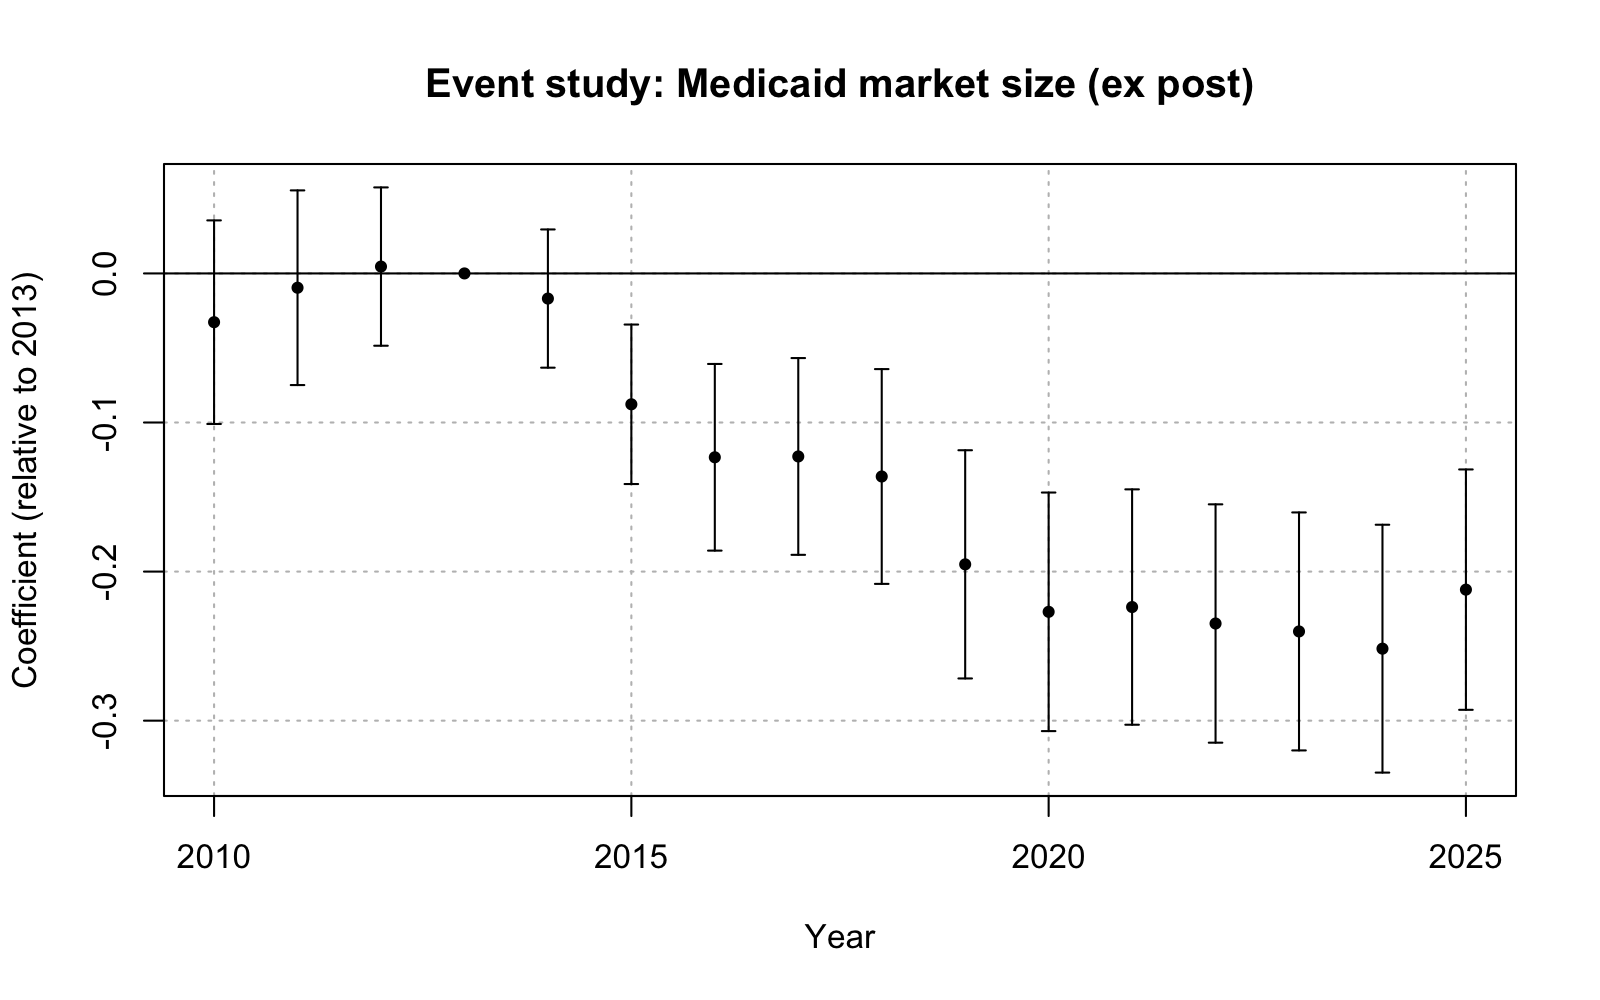
\includegraphics[width=\linewidth]{../output/RQ2/patent_feols_expost_medicaid.png}
  \caption{FEOLS event study: patents, Medicaid exposure (ex-post)}
  \label{fig:rob_rq2_patent_expost_medicaid}
\end{figure}

\begin{figure}[!h]
  \centering
  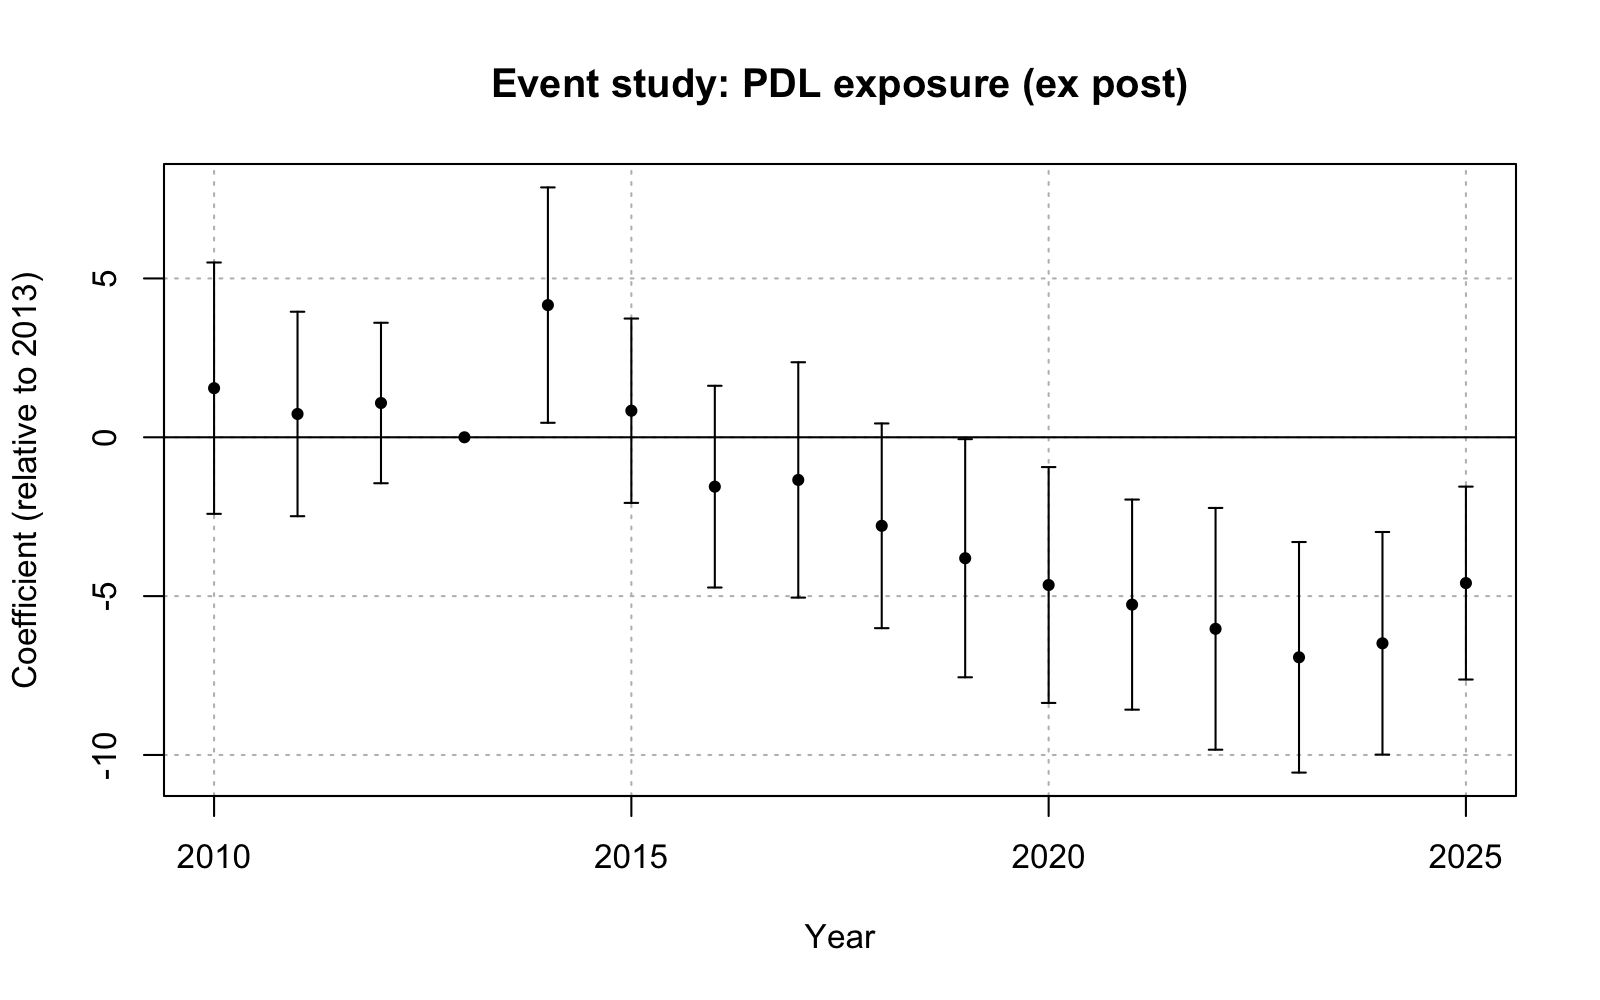
\includegraphics[width=\linewidth]{../output/RQ2/patent_feols_expost_pdl.png}
  \caption{FEOLS event study: patents, PDL exposure (ex-post)}
  \label{fig:rob_rq2_patent_expost_pdl}
\end{figure}

\clearpage

\begin{figure}[!h]
  \centering
  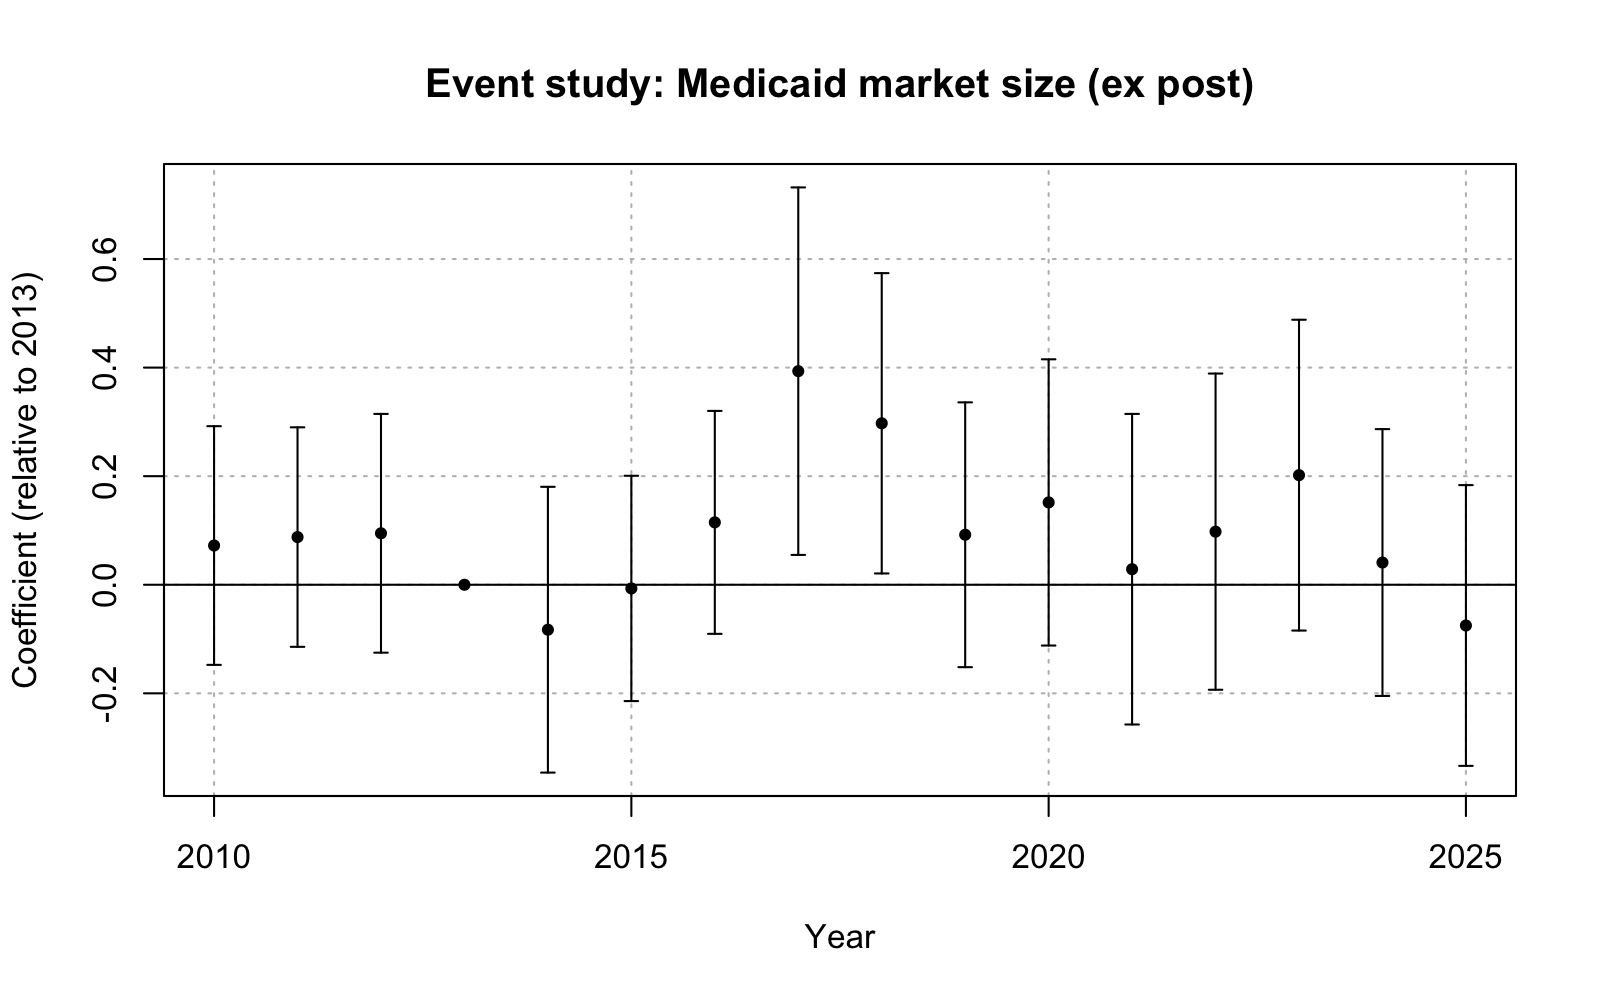
\includegraphics[width=\linewidth]{../output/RQ2/fda_feols_expost_medicaid.png}
  \caption{FEOLS event study: FDA approvals, Medicaid exposure (ex-post)}
  \label{fig:rob_rq2_fda_expost_medicaid}
\end{figure}

\begin{figure}[!h]
  \centering
  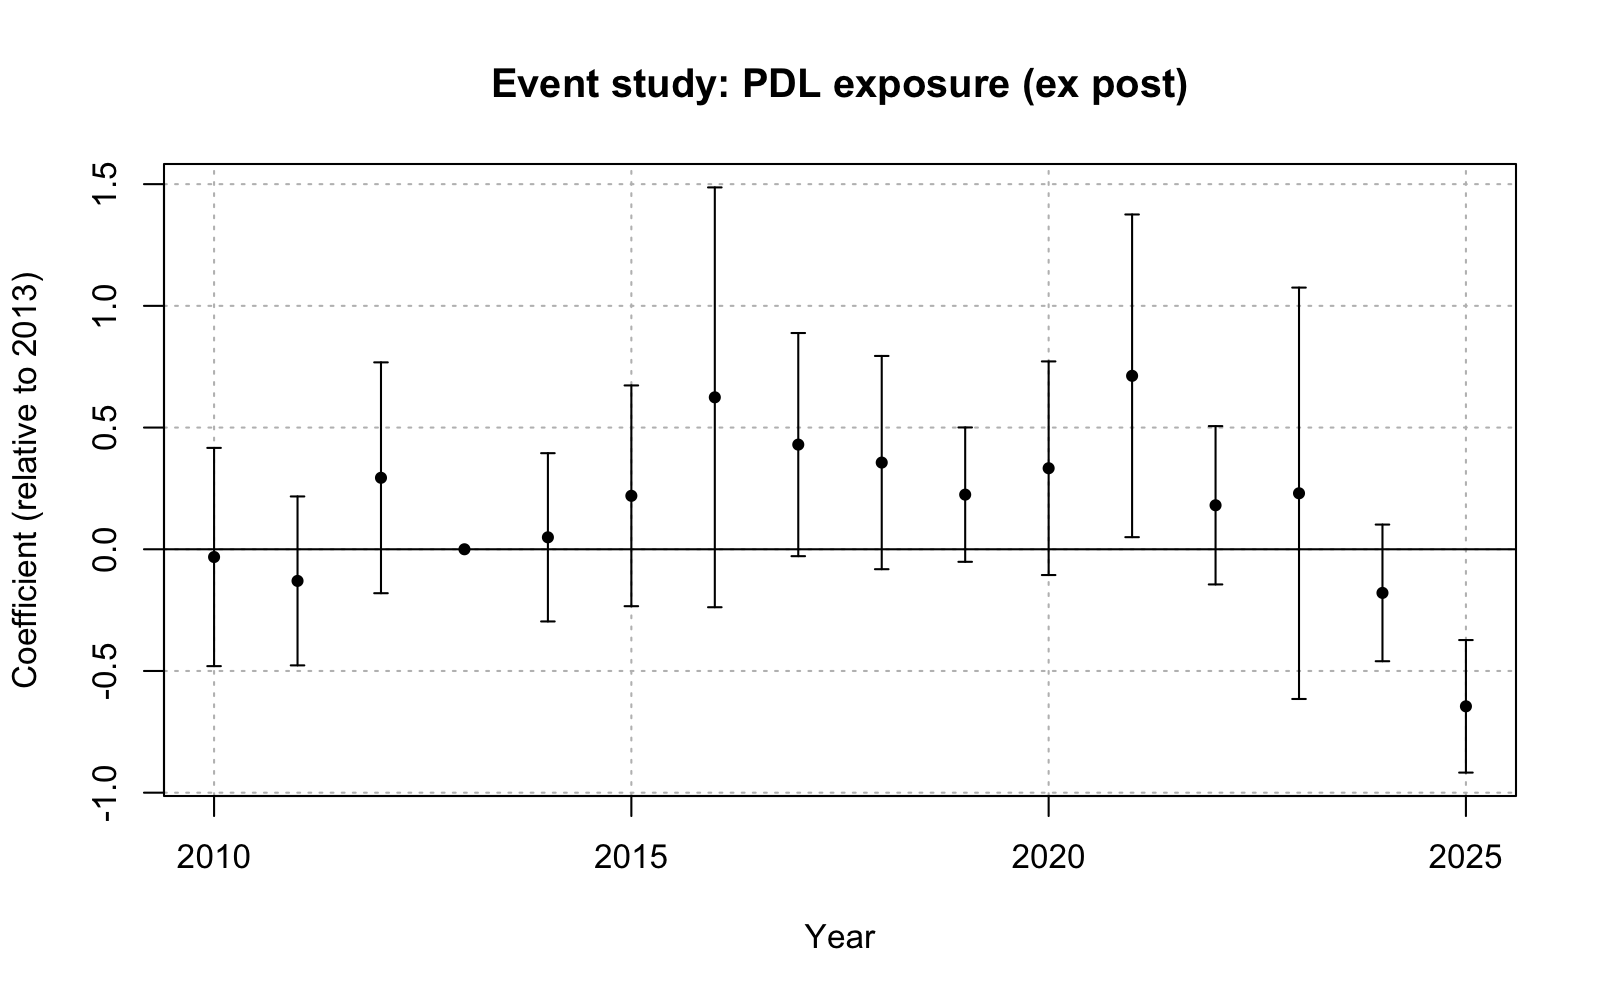
\includegraphics[width=\linewidth]{../output/RQ2/fda_feols_expost_pdl.png}
  \caption{FEOLS event study: FDA approvals, PDL exposure (ex-post)}
  \label{fig:rob_rq2_fda_expost_pdl}
\end{figure}

\clearpage

% -----------------------------------------------------------------------
\subsection{RQ3: Therapeutic-Class Heterogeneity}
% -----------------------------------------------------------------------

\subsubsection{Ex-Post Medicaid Exposure}

The RQ3 specification allows for heterogeneity in innovation behaviour to vary at ATC Level 1 therapeutic class. The ex-post exposure measure of Medicaid exposure is used as a robustness check.

\begin{center}
\begingroup\footnotesize
\begin{table}
\centering
\begin{talltblr}[         %% tabularray outer open
entry=none,label=none,
note{}={* p \num{< 0.05}, ** p \num{< 0.01}, *** p \num{< 0.001}},
]                     %% tabularray outer close
{                     %% tabularray inner open
colspec={Q[]Q[]Q[]},
column{2,3}={}{halign=c,},
column{1}={}{halign=l,},
hline{26}={1,2,3}{solid, black, 0.05em},
}                     %% tabularray inner close
\toprule
& Patents & FDA Approvals \\ \midrule
Medicaid Share × ATC = A & \num{-0.157}*** & \num{1.301}**  \\
& (\num{0.031})   & (\num{0.420})  \\
Medicaid Share × ATC = B & \num{0.151}***  & \num{-0.121}   \\
& (\num{0.027})   & (\num{0.784})  \\
Medicaid Share × ATC = C & \num{-0.094}*** & \num{0.373}    \\
& (\num{0.015})   & (\num{0.278})  \\
Medicaid Share × ATC = D & \num{-0.017}    & \num{0.881}**  \\
& (\num{0.062})   & (\num{0.337})  \\
Medicaid Share × ATC = G & \num{0.032}     & \num{-1.058}   \\
& (\num{0.049})   & (\num{1.121})  \\
Medicaid Share × ATC = H & \num{0.619}***  & \num{0.446}    \\
& (\num{0.096})   & (\num{0.530})  \\
Medicaid Share × ATC = J & \num{0.035}     & \num{-0.078}   \\
& (\num{0.034})   & (\num{0.089})  \\
Medicaid Share × ATC = L & \num{0.443}     & \num{-0.244}   \\
& (\num{0.578})   & (\num{2.115})  \\
Medicaid Share × ATC = M & \num{-0.212}*** & \num{0.017}    \\
& (\num{0.048})   & (\num{0.858})  \\
Medicaid Share × ATC = N & \num{-0.174}*** & \num{0.047}    \\
& (\num{0.039})   & (\num{0.101})  \\
Medicaid Share × ATC = R & \num{0.005}     & \num{0.178}    \\
& (\num{0.003})   & (\num{0.130})  \\
Medicaid Share × ATC = S & \num{0.105}***  & \num{6.473}*   \\
& (\num{0.020})   & (\num{3.004})  \\
Num. obs.                & \num{19617728}  & \num{561600}   \\
R2                       & \num{0.247}     & \num{0.235}    \\
\bottomrule
\end{talltblr}
\end{table}

\endgroup
\end{center}


The ex-post estimates are broadly consistent with the ex-ante baseline. Therapeutic classes that exhibited significant negative patent responses under ex-ante exposure, continue to display significant negative coefficients under the ex-post measure. Additionally, positive patent responses are still observed for therapeutic classes relating to blood related drugs, hormonal preparations, and sensory organs. Simiarly, the FDA approval coefficients are aligned with their ex-ante results - significant positive responses for alimentary tract and dermatologicals, and no class are recorded to have a significant reduction in approvals. The results aligning between the two exposure measures indicates that the baseline class-level heterogeneity in innovation response is not driven by the choice of exposure measure.

\subsubsection{Parallel Trends}

The RQ3 triple-difference specification does not take the form of an event study, as the estimation of class-specific dynamic coefficients would be computationally intensive. Consequently, pre-trends coefficients cannot be estimated directly, so the parallel trends assumption cannot be tested for in the same manner as RQ1 and RQ2. Since ATC class V is the omitted from the regressions, it is the reference group for the DDD models. In this context, this specifically indicates that absent the ACA, the relationship between Medicaid exposure and changes in innovation outcomes would have evolved similarly across therapeutic classes relative to class V. The results from earlier the earlier analyses and the model structure can provide evidence to support the plausibility of this assumption.

First, the RQ1 and RQ2 event studies consistently display small and statistically insignificant pre-expansion coefficients across all specifications, including FEOLS, FE Poisson, binned treatment and the continuous DiD approach. Therefore, therapeutic classes with differing levels of Medicaid exposure followed similar innovation trajectories prior to the ACA expansion. Since the same Medicaid exposure measure and firm-class panels are used for RQ3, the evidence for parallel trends from RQ1 and RQ2 provide support for the key identifying assumption of RQ3.

Third, as discussed in the methodology, a violation of parallel trends would require an additional shock around 2014 that differentially affected innovation within therapeutic classes such that it was correlated with exposure to Medicaid. There are no clear candidates for such a confounding shock.

\clearpage

\bibliographystyle{apalike}
\bibliography{references}

\clearpage
\appendix

% -----------------------------------------------------------------------
\section{Robustness Regression Tables}
% -----------------------------------------------------------------------

\subsection{RQ1: Ex-Post FEOLS}

\begingroup\footnotesize
\begin{table}
\centering
\begin{talltblr}[         %% tabularray outer open
entry=none,label=none,
note{}={* p \num{< 0.05}, ** p \num{< 0.01}, *** p \num{< 0.001}},
]                     %% tabularray outer close
{                     %% tabularray inner open
width=\linewidth,
colspec={Q[]X[]X[]},
column{2,3}={}{halign=c,},
column{1}={}{halign=l,},
hline{32}={1,2,3}{solid, black, 0.05em},
}                     %% tabularray inner close
\toprule
& Patents & FDA Approvals \\ \midrule
2010 × Medicaid Share & \num{-0.033}    & \num{0.286}   \\
                      & (\num{0.035})   & (\num{0.450}) \\
2011 × Medicaid Share & \num{-0.010}    & \num{0.336}   \\
                      & (\num{0.033})   & (\num{0.413}) \\
2012 × Medicaid Share & \num{0.004}     & \num{0.414}   \\
                      & (\num{0.027})   & (\num{0.455}) \\
2014 × Medicaid Share & \num{-0.018}    & \num{-0.324}  \\
                      & (\num{0.024})   & (\num{0.533}) \\
2015 × Medicaid Share & \num{-0.088}**  & \num{0.005}   \\
                      & (\num{0.027})   & (\num{0.420}) \\
2016 × Medicaid Share & \num{-0.123}*** & \num{0.550}   \\
                      & (\num{0.032})   & (\num{0.413}) \\
2017 × Medicaid Share & \num{-0.122}*** & \num{1.635}*  \\
                      & (\num{0.034})   & (\num{0.688}) \\
2018 × Medicaid Share & \num{-0.135}*** & \num{1.240}*  \\
                      & (\num{0.037})   & (\num{0.560}) \\
2019 × Medicaid Share & \num{-0.194}*** & \num{0.400}   \\
                      & (\num{0.039})   & (\num{0.497}) \\
2020 × Medicaid Share & \num{-0.225}*** & \num{0.652}   \\
                      & (\num{0.041})   & (\num{0.529}) \\
2021 × Medicaid Share & \num{-0.222}*** & \num{0.218}   \\
                      & (\num{0.040})   & (\num{0.573}) \\
2022 × Medicaid Share & \num{-0.233}*** & \num{0.418}   \\
                      & (\num{0.040})   & (\num{0.590}) \\
2023 × Medicaid Share & \num{-0.238}*** & \num{0.842}   \\
                      & (\num{0.040})   & (\num{0.576}) \\
2024 × Medicaid Share & \num{-0.250}*** & \num{0.137}   \\
                      & (\num{0.042})   & (\num{0.502}) \\
2025 × Medicaid Share & \num{-0.212}*** & \num{-0.380}  \\
                      & (\num{0.041})   & (\num{0.531}) \\
Num. obs.             & \num{5281696}   & \num{151200}  \\
R2                    & \num{0.534}     & \num{0.609}   \\
\bottomrule
\end{talltblr}
\end{table}

\endgroup

\clearpage

\subsection{RQ1: FE Poisson (Ex-Ante)}

\begingroup\footnotesize
\begin{table}
\centering
\begin{talltblr}[         %% tabularray outer open
entry=none,label=none,
note{}={* p \num{< 0.05}, ** p \num{< 0.01}, *** p \num{< 0.001}},
]                     %% tabularray outer close
{                     %% tabularray inner open
width=\linewidth,
colspec={Q[]X[]X[]},
column{2,3}={}{halign=c,},
column{1}={}{halign=l,},
hline{32}={1,2,3}{solid, black, 0.05em},
}                     %% tabularray inner close
\toprule
& Patents & FDA Approvals \\ \midrule
2010 × Medicaid Share & \num{0.120}     & \num{0.237}   \\
                      & (\num{0.154})   & (\num{0.636}) \\
2011 × Medicaid Share & \num{0.218}     & \num{0.326}   \\
                      & (\num{0.140})   & (\num{0.446}) \\
2012 × Medicaid Share & \num{0.115}     & \num{0.643}   \\
                      & (\num{0.108})   & (\num{0.615}) \\
2014 × Medicaid Share & \num{-0.092}    & \num{-0.545}  \\
                      & (\num{0.108})   & (\num{0.638}) \\
2015 × Medicaid Share & \num{-0.300}*   & \num{-0.434}  \\
                      & (\num{0.118})   & (\num{0.632}) \\
2016 × Medicaid Share & \num{-0.435}*** & \num{-0.834}  \\
                      & (\num{0.124})   & (\num{0.478}) \\
2017 × Medicaid Share & \num{-0.397}**  & \num{-0.495}  \\
                      & (\num{0.131})   & (\num{0.480}) \\
2018 × Medicaid Share & \num{-0.415}**  & \num{-0.772}  \\
                      & (\num{0.149})   & (\num{0.530}) \\
2019 × Medicaid Share & \num{-0.784}*** & \num{-0.381}  \\
                      & (\num{0.154})   & (\num{0.565}) \\
2020 × Medicaid Share & \num{-0.998}*** & \num{-0.733}  \\
                      & (\num{0.173})   & (\num{0.574}) \\
2021 × Medicaid Share & \num{-0.989}*** & \num{-0.867}  \\
                      & (\num{0.170})   & (\num{0.729}) \\
2022 × Medicaid Share & \num{-1.137}*** & \num{-0.637}  \\
                      & (\num{0.186})   & (\num{0.594}) \\
2023 × Medicaid Share & \num{-1.324}*** & \num{-0.566}  \\
                      & (\num{0.201})   & (\num{0.511}) \\
2024 × Medicaid Share & \num{-1.474}*** & \num{-0.680}  \\
                      & (\num{0.261})   & (\num{0.573}) \\
2025 × Medicaid Share & \num{-1.110}*** & \num{-0.668}  \\
                      & (\num{0.229})   & (\num{0.580}) \\
Num. obs.             & \num{1300944}   & \num{42176}   \\
\bottomrule
\end{talltblr}
\end{table}

\endgroup

\clearpage

\subsection{RQ1: FE Poisson (Ex-Post)}

\begingroup\footnotesize
\begin{table}
\centering
\begin{talltblr}[         %% tabularray outer open
entry=none,label=none,
note{}={* p \num{< 0.05}, ** p \num{< 0.01}, *** p \num{< 0.001}},
]                     %% tabularray outer close
{                     %% tabularray inner open
width=\linewidth,
colspec={Q[]X[]X[]},
column{2,3}={}{halign=c,},
column{1}={}{halign=l,},
hline{32}={1,2,3}{solid, black, 0.05em},
}                     %% tabularray inner close
\toprule
& Patents & FDA Approvals \\ \midrule
2010 × Medicaid Share & \num{0.129}     & \num{0.453}   \\
                      & (\num{0.157})   & (\num{0.869}) \\
2011 × Medicaid Share & \num{0.240}     & \num{1.138}   \\
                      & (\num{0.145})   & (\num{0.687}) \\
2012 × Medicaid Share & \num{0.124}     & \num{1.250}   \\
                      & (\num{0.115})   & (\num{0.863}) \\
2014 × Medicaid Share & \num{-0.086}    & \num{-0.711}  \\
                      & (\num{0.106})   & (\num{0.996}) \\
2015 × Medicaid Share & \num{-0.367}**  & \num{-0.431}  \\
                      & (\num{0.119})   & (\num{0.725}) \\
2016 × Medicaid Share & \num{-0.515}*** & \num{-0.788}  \\
                      & (\num{0.129})   & (\num{0.660}) \\
2017 × Medicaid Share & \num{-0.533}*** & \num{-0.278}  \\
                      & (\num{0.134})   & (\num{0.735}) \\
2018 × Medicaid Share & \num{-0.556}*** & \num{-0.595}  \\
                      & (\num{0.157})   & (\num{0.713}) \\
2019 × Medicaid Share & \num{-0.998}*** & \num{-0.625}  \\
                      & (\num{0.167})   & (\num{0.764}) \\
2020 × Medicaid Share & \num{-1.293}*** & \num{-0.916}  \\
                      & (\num{0.190})   & (\num{0.839}) \\
2021 × Medicaid Share & \num{-1.313}*** & \num{-0.909}  \\
                      & (\num{0.188})   & (\num{0.910}) \\
2022 × Medicaid Share & \num{-1.564}*** & \num{-0.657}  \\
                      & (\num{0.203})   & (\num{0.775}) \\
2023 × Medicaid Share & \num{-1.803}*** & \num{-0.618}  \\
                      & (\num{0.224})   & (\num{0.695}) \\
2024 × Medicaid Share & \num{-2.021}*** & \num{-0.969}  \\
                      & (\num{0.266})   & (\num{0.854}) \\
2025 × Medicaid Share & \num{-1.692}*** & \num{-1.254}  \\
                      & (\num{0.262})   & (\num{0.892}) \\
Num. obs.             & \num{1300944}   & \num{42176}   \\
\bottomrule
\end{talltblr}
\end{table}

\endgroup

\begin{figure}[!h]
  \centering
  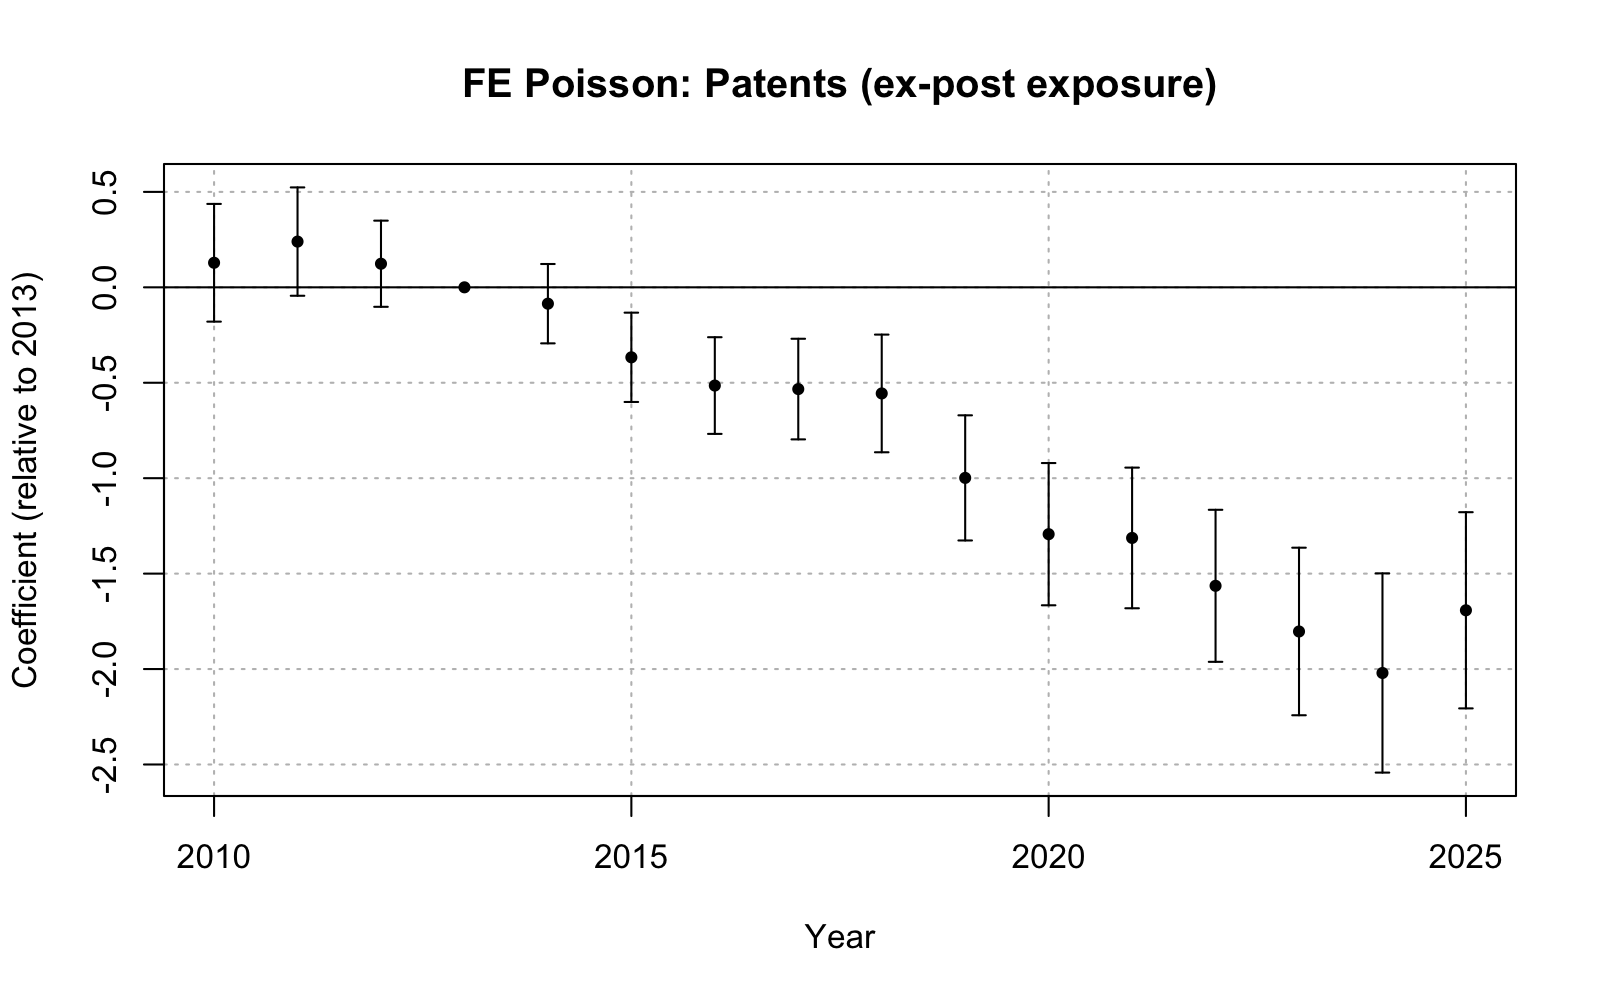
\includegraphics[width=\linewidth]{../output/RQ1/patent_poi_expost.png}
  \caption{FE Poisson event study: patents, ex-post Medicaid exposure}
  \label{fig:rob_rq1_patent_poi_expost}
\end{figure}

\begin{figure}[!h]
  \centering
  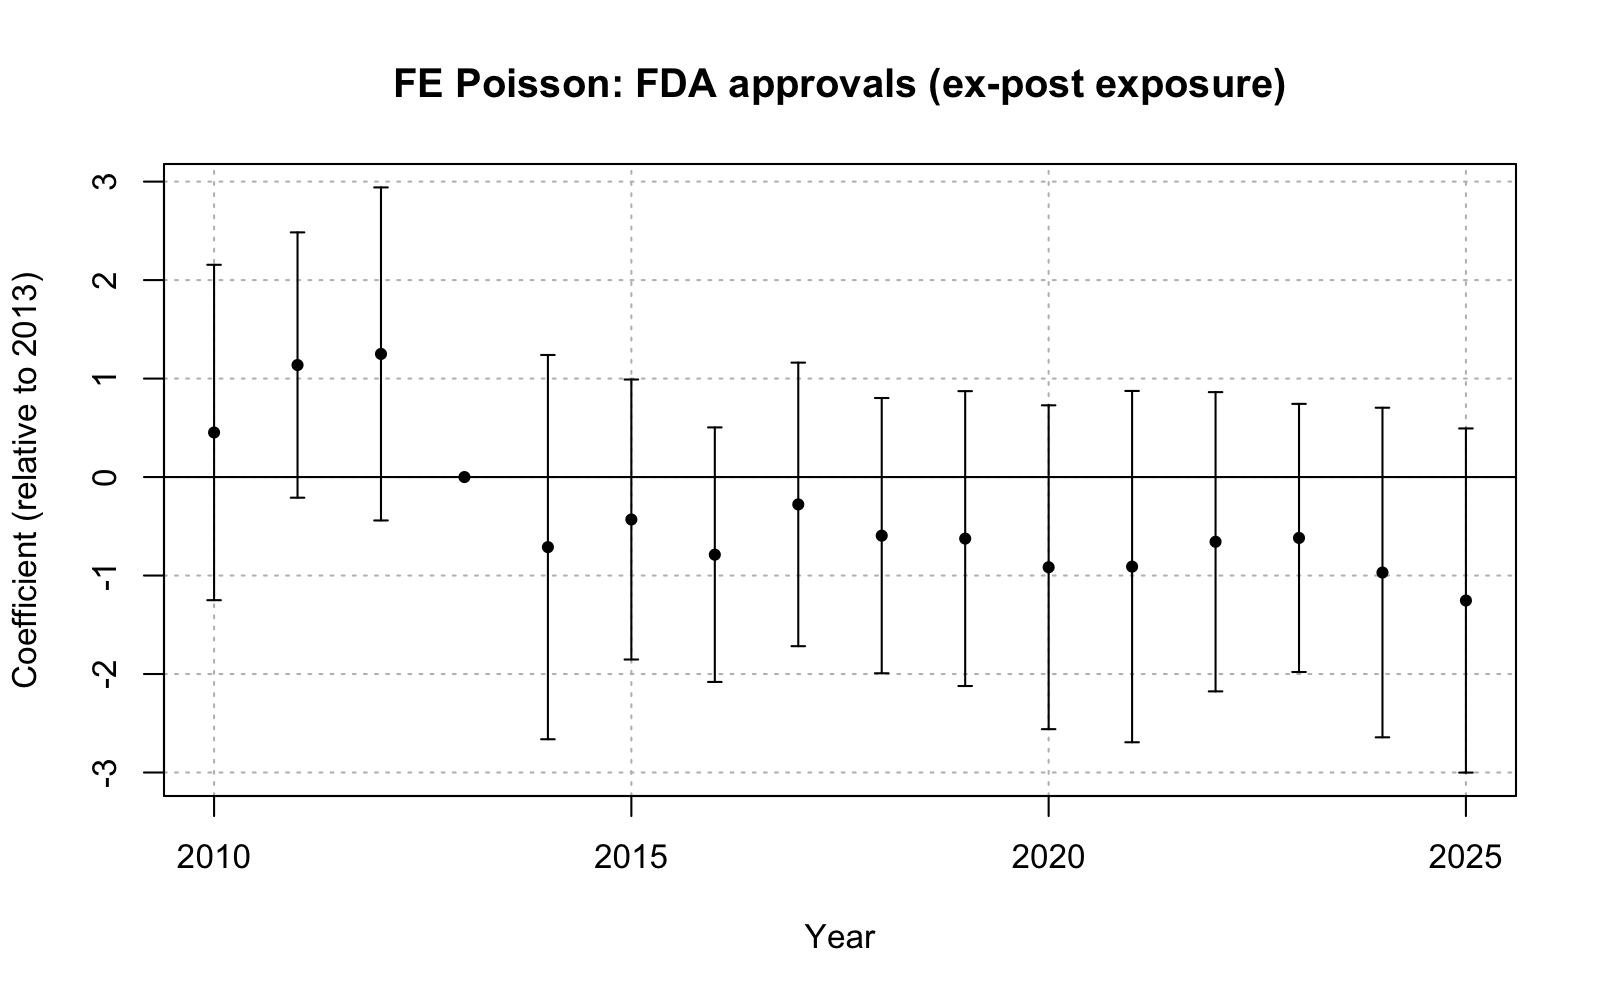
\includegraphics[width=\linewidth]{../output/RQ1/fda_poi_expost.png}
  \caption{FE Poisson event study: FDA approvals, ex-post Medicaid exposure}
  \label{fig:rob_rq1_fda_poi_expost}
\end{figure}

\clearpage

\subsection{RQ1: Binned Treatment}

\begingroup\footnotesize
\begin{table}
\centering
\begin{talltblr}[         %% tabularray outer open
entry=none,label=none,
note{}={* p \num{< 0.05}, ** p \num{< 0.01}, *** p \num{< 0.001}},
]                     %% tabularray outer close
{                     %% tabularray inner open
width=\linewidth,
colspec={Q[]X[]X[]X[]X[]},
column{2,3,4,5}={}{halign=c,},
column{1}={}{halign=l,},
hline{33}={1,2,3,4,5}{solid, black, 0.05em},
}                     %% tabularray inner close
\toprule
& \SetCell[c=2]{c} Patents && \SetCell[c=2]{c} FDA Approvals & \\
& Medium Bin & High Bin & Medium Bin & High Bin \\ \midrule
2010 & \num{-0.008}    & \num{-0.029}    & \num{0.042}   & \num{0.085}   \\
     & (\num{0.006})   & (\num{0.017})   & (\num{0.055}) & (\num{0.140}) \\
2011 & \num{-0.005}    & \num{-0.025}    & \num{0.058}   & \num{-0.064}  \\
     & (\num{0.006})   & (\num{0.016})   & (\num{0.065}) & (\num{0.105}) \\
2012 & \num{0.009}     & \num{-0.003}    & \num{0.042}   & \num{0.033}   \\
     & (\num{0.006})   & (\num{0.012})   & (\num{0.077}) & (\num{0.121}) \\
2014 & \num{0.015}**   & \num{-0.002}    & \num{0.047}   & \num{-0.091}  \\
     & (\num{0.005})   & (\num{0.011})   & (\num{0.067}) & (\num{0.130}) \\
2015 & \num{0.002}     & \num{-0.027}*   & \num{0.006}   & \num{-0.005}  \\
     & (\num{0.005})   & (\num{0.013})   & (\num{0.073}) & (\num{0.148}) \\
2016 & \num{0.007}     & \num{-0.058}*** & \num{0.158}   & \num{0.070}   \\
     & (\num{0.006})   & (\num{0.014})   & (\num{0.101}) & (\num{0.130}) \\
2017 & \num{0.005}     & \num{-0.047}**  & \num{0.239}*  & \num{0.326}   \\
     & (\num{0.006})   & (\num{0.015})   & (\num{0.114}) & (\num{0.181}) \\
2018 & \num{-0.009}    & \num{-0.075}*** & \num{0.185}*  & \num{0.213}   \\
     & (\num{0.006})   & (\num{0.017})   & (\num{0.093}) & (\num{0.155}) \\
2019 & \num{-0.004}    & \num{-0.092}*** & \num{0.071}   & \num{0.206}   \\
     & (\num{0.007})   & (\num{0.017})   & (\num{0.077}) & (\num{0.162}) \\
2020 & \num{-0.003}    & \num{-0.108}*** & \num{0.012}   & \num{0.141}   \\
     & (\num{0.006})   & (\num{0.018})   & (\num{0.092}) & (\num{0.142}) \\
2021 & \num{-0.005}    & \num{-0.118}*** & \num{0.127}   & \num{-0.048}  \\
     & (\num{0.006})   & (\num{0.018})   & (\num{0.105}) & (\num{0.182}) \\
2022 & \num{-0.010}    & \num{-0.129}*** & \num{0.101}   & \num{0.040}   \\
     & (\num{0.006})   & (\num{0.018})   & (\num{0.075}) & (\num{0.184}) \\
2023 & \num{-0.011}    & \num{-0.141}*** & \num{0.152}   & \num{0.154}   \\
     & (\num{0.006})   & (\num{0.019})   & (\num{0.087}) & (\num{0.182}) \\
2024 & \num{-0.005}    & \num{-0.142}*** & \num{0.037}   & \num{0.070}   \\
     & (\num{0.010})   & (\num{0.019})   & (\num{0.066}) & (\num{0.146}) \\
2025 & \num{-0.020}**  & \num{-0.155}*** & \num{0.010}   & \num{0.032}   \\
     & (\num{0.006})   & (\num{0.019})   & (\num{0.067}) & (\num{0.153}) \\
Num. obs. & \SetCell[c=2]{c} \num{5281696} && \SetCell[c=2]{c} \num{151200} & \\
R2        & \SetCell[c=2]{c} \num{0.534}   && \SetCell[c=2]{c} \num{0.609}  & \\
\bottomrule
\end{talltblr}
\end{table}

\endgroup

\clearpage

\subsection{RQ1: Continuous Difference-in-Differences}

\begingroup
\makeatletter
\renewenvironment{table}[1][tbp]{\@float{table}[#1]}{\end@float}
\makeatother
\footnotesize
\begin{table}
\centering
\begin{talltblr}[         %% tabularray outer open
entry=none,label=none,
note{}={* 95\% uniform confidence band does not cover 0},
]                     %% tabularray outer close
{                     %% tabularray inner open
colspec={Q[]Q[]Q[]},
column{2,3}={}{halign=c,},
column{1}={}{halign=l,},
hline{8}={1,2,3}{solid, black, 0.05em},
}                     %% tabularray inner close
\toprule
Event Time & Patents & FDA Approvals \\ \midrule %% TinyTableHeader
-3 & \num{0.0038} & \num{-0.0368} \\
   & (\num{0.0034}) & (\num{0.0602}) \\
-2 & \num{0.0023} & \num{0.0361} \\
   & (\num{0.0037}) & (\num{0.0576}) \\
-1 & \num{0.0002} & \num{-0.0326} \\
   & (\num{0.0050}) & (\num{0.0632}) \\
0 & \num{-0.0025} & \num{-0.0506} \\
   & (\num{0.0044}) & (\num{0.0731}) \\
1 & \num{-0.0126} & \num{-0.0092} \\
   & (\num{0.0055}) & (\num{0.0706}) \\
2 & \num{-0.0181}* & \num{0.0646} \\
   & (\num{0.0062}) & (\num{0.0721}) \\
3 & \num{-0.0165} & \num{0.2233} \\
   & (\num{0.0069}) & (\num{0.1018}) \\
4 & \num{-0.0189} & \num{0.1568} \\
   & (\num{0.0073}) & (\num{0.0930}) \\
5 & \num{-0.0271}* & \num{0.0861} \\
   & (\num{0.0080}) & (\num{0.0866}) \\
6 & \num{-0.0313}* & \num{0.1151} \\
   & (\num{0.0082}) & (\num{0.0846}) \\
7 & \num{-0.0315}* & \num{0.0223} \\
   & (\num{0.0084}) & (\num{0.1022}) \\
8 & \num{-0.0333}* & \num{0.0579} \\
   & (\num{0.0083}) & (\num{0.1086}) \\
9 & \num{-0.0348}* & \num{0.1329} \\
   & (\num{0.0084}) & (\num{0.1056}) \\
10 & \num{-0.0358}* & \num{0.0404} \\
   & (\num{0.0085}) & (\num{0.0921}) \\
11 & \num{-0.0324}* & \num{-0.0213} \\
   & (\num{0.0091}) & (\num{0.0919}) \\
\bottomrule
\end{talltblr}
\end{table}

\endgroup

\clearpage

\subsection{RQ2: Ex-Post FEOLS}

\begingroup\footnotesize
\begin{table}
\centering
\begin{talltblr}[         %% tabularray outer open
entry=none,label=none,
note{}={* p \num{< 0.05}, ** p \num{< 0.01}, *** p \num{< 0.001}},
]                     %% tabularray outer close
{                     %% tabularray inner open
width=\linewidth,
colspec={Q[]X[]X[]X[]X[]},
column{2,3,4,5}={}{halign=c,},
column{1}={}{halign=l,},
hline{33}={1,2,3,4,5}{solid, black, 0.05em},
}                     %% tabularray inner close
\toprule
& \SetCell[c=2]{c} Patents && \SetCell[c=2]{c} FDA Approvals & \\
& Medicaid Market Share & PDL Exposure & Medicaid Market Share & PDL Exposure \\ \midrule
2010 & \num{-0.033}    & \num{1.546}     & \num{0.285}   & \num{0.046}   \\
     & (\num{0.035})   & (\num{2.018})   & (\num{0.448}) & (\num{0.807}) \\
2011 & \num{-0.010}    & \num{0.734}     & \num{0.344}   & \num{-0.257}  \\
     & (\num{0.033})   & (\num{1.642})   & (\num{0.412}) & (\num{0.711}) \\
2012 & \num{0.005}     & \num{1.079}     & \num{0.371}   & \num{1.395}   \\
     & (\num{0.027})   & (\num{1.289})   & (\num{0.447}) & (\num{0.912}) \\
2014 & \num{-0.017}    & \num{4.161}*    & \num{-0.338}  & \num{0.398}   \\
     & (\num{0.024})   & (\num{1.890})   & (\num{0.536}) & (\num{0.647}) \\
2015 & \num{-0.088}**  & \num{0.836}     & \num{-0.037}  & \num{1.158}   \\
     & (\num{0.027})   & (\num{1.480})   & (\num{0.422}) & (\num{0.881}) \\
2016 & \num{-0.123}*** & \num{-1.554}    & \num{0.456}   & \num{2.642}   \\
     & (\num{0.032})   & (\num{1.620})   & (\num{0.418}) & (\num{1.682}) \\
2017 & \num{-0.123}*** & \num{-1.342}    & \num{1.566}*  & \num{1.924}   \\
     & (\num{0.034})   & (\num{1.890})   & (\num{0.690}) & (\num{0.992}) \\
2018 & \num{-0.136}*** & \num{-2.787}    & \num{1.181}*  & \num{1.683}   \\
     & (\num{0.037})   & (\num{1.644})   & (\num{0.563}) & (\num{1.021}) \\
2019 & \num{-0.195}*** & \num{-3.807}*   & \num{0.359}   & \num{1.171}*  \\
     & (\num{0.039})   & (\num{1.912})   & (\num{0.498}) & (\num{0.591}) \\
2020 & \num{-0.227}*** & \num{-4.650}*   & \num{0.598}   & \num{1.585}   \\
     & (\num{0.041})   & (\num{1.894})   & (\num{0.537}) & (\num{0.942}) \\
2021 & \num{-0.224}*** & \num{-5.267}**  & \num{0.103}   & \num{3.110}*  \\
     & (\num{0.040})   & (\num{1.687})   & (\num{0.583}) & (\num{1.393}) \\
2022 & \num{-0.235}*** & \num{-6.029}**  & \num{0.381}   & \num{0.994}   \\
     & (\num{0.041})   & (\num{1.941})   & (\num{0.593}) & (\num{0.653}) \\
2023 & \num{-0.240}*** & \num{-6.926}*** & \num{0.798}   & \num{1.191}   \\
     & (\num{0.041})   & (\num{1.851})   & (\num{0.583}) & (\num{1.737}) \\
2024 & \num{-0.252}*** & \num{-6.485}*** & \num{0.154}   & \num{-0.447}  \\
     & (\num{0.042})   & (\num{1.788})   & (\num{0.501}) & (\num{0.589}) \\
2025 & \num{-0.212}*** & \num{-4.589}**  & \num{-0.347}  & \num{-1.113}  \\
     & (\num{0.041})   & (\num{1.549})   & (\num{0.525}) & (\num{0.908}) \\
Num. obs. & \SetCell[c=2]{c} \num{5281696} && \SetCell[c=2]{c} \num{151200} & \\
R2        & \SetCell[c=2]{c} \num{0.535}   && \SetCell[c=2]{c} \num{0.609}  & \\
\bottomrule
\end{talltblr}
\end{table}

\endgroup

\end{document}

\input{theoretical_model}
\documentclass[12pt]{article}
\usepackage{geometry}
\geometry{a4paper, portrait, margin=1in}

% --- Math Packages ---
\usepackage{amsmath}
\usepackage{amssymb}
\usepackage{amsfonts}
\usepackage{amsthm}

% --- Graphics & Diagrams ---
\usepackage{graphicx}
\usepackage{tikz}
\usetikzlibrary{shapes, arrows, positioning}

% --- Formatting ---
\usepackage{parskip}
\usepackage[hidelinks]{hyperref}
\usepackage{natbib}
\usepackage{enumitem}
\pagestyle{plain}

% --- Word count (requires compiling with --shell-escape) ---
\newcommand{\wordcount}{%
  \immediate\write18{texcount -sum -1 \jobname.tex 2>/dev/null | python3 -c "import sys; n=sys.stdin.read().strip(); print(f'{int(n):,}') if n.isdigit() else print('?')" > \jobname.wc}%
  \input{\jobname.wc}%
}

\title{MPhil Thesis: Conclusion}
\author{Mohammad-Shah Karim}
\date{May 2026}

\begin{document}

\ifdefined\isdraft\else
\maketitle
\begin{center}
  \small Word count: \wordcount
\end{center}
\fi

\section{Directions for Further Research}

The empirical and theoretical analysis presented in this thesis is subject to several limitations. This section discusses the most important of these and identifies directions in which future work could extend the analysis.

\subsection{Clinical Trial Outcomes}

This thesis chooses to study patenting and drug approvals to capture the innovation stages before and after clinical-trials studied by \citet{NBERw28755}. Clinical trials are an intermediate position between these two outcomes; incorporating clinical-trial data would complete the pipeline comparison, thereby allowing the analysis to trace the innovation response across all three stages. Given the scope of this study, this extension was not feasible within the scope of the present study. \citeauthor{NBERw28755} utilise a proprietary clinical trial data supplied by Cortellis. Constructing a comparable panel from ClinicalTrials.gov would require substantial work. The wording of study titles vary substantially and do not always identify the relevant disease area explicitly. Mapping these records to therapeutic-classes would therefore require imperfect text-based classification. Future work utilising Cortellis could assess whether the negative patenting response identified in this thesis is mirrored at the trial stage.

\subsection{PDL Measurement}

The PDL exposure measure used in this thesis is constructed from the Texas Vendor Drug Program, as this is the only state that has made the full formulary history available in a machine-readable format. While the representativeness analysis indicates that the Texas PDL shares substantial overlap with the New York and Washington, overlap with California is considerably weaker, reflecting differences in state-level formulary structures. This introduces measurement error into the PDL exposure variable, since firms classified as having heavy exposure to the PDL in Texas may be less exposed to it in other states. Consequently, the estimated innovations response to PDL exposure is likely to be attenuated towards zero, and should be interpreted as a plausible lower bound. Further work could construct a multi-state PDL exposure measure using additional formulary records, and average these across states to obtain a more representative measure ofa firm's overall exposure to Medicaid's PDL.

\subsection{Therapeutic Classification}

The analysis aggregates all outcomes to a coarse clinical outcome - ATC Level 1. This can contain drugs with substantially different clinical profiles and competitive environments, so within-class innovation heterogeneity may be masked. This is particularly relevant for the heterogeneity analysis in RQ3, where differences in innovation responses may remain hidden even where the ATC Level 1 estimates appear null or weak. Finer classification such as ATC Levels 2 or 3 may allow the analysis to distinguish between sub-therapeutic areas, but would come at the cost of an increase in panel dimensionality and therefore computational demands. Patents are classified using a CPC-to-ATC crosswalk, and extending to more granular ATC levels would require a mapping that may be noisy.

\subsection{Alternative Estimators for the Joint Specification}

The FE Poisson, binned-treatment, and continuous DiD estimators are applied to the RQ1 specification but not the RQ2 specification separating the innovation responses to both Medicaid and PDL exposure. Extending these estimators to the joint specification exceeded the computational power of the device used for this thesis, due to the size of the firm-class panels and the additional interactions required. The RQ2 estimates are instead supported by the ex-ante and ex-post exposure comparison with the use of FEOLS, but were not subject to equivalent estimator-level sensitivity analysis. Future work could therefore use greater computational capacity to assess whether the decomposition of demand and PDL exposure is robust alternative models.

\subsection{The Theoretical Model}

The theoretical model developed is an illustrative simplification designed to formalise how the Medicaid expansion can reduce innovation incentives through the procurement design. The model restricts competition to two firms competing for access within each therapeutic class, and assumes that the winner of the price stage receives the entire Medicaid market. In reality, several manufacturers compete for PDL authorisation within a therapeutic class, and multiple products may receive preferred placement. The model therefore abstracts from an oligopolistic structure to a duopoly setting in order to isolate the interaction between market size, rebate extraction, and the rent gap rather than the exact number of firms. An $N$-firm extension would allow for the examination of how rebate pressure scales with the number of clinically viable competitors, and whether the Medicaid expansion causes marginal firms to exit Medicaid-relevant therapeutic areas entirely rather than simply reducing innovation effort.

\section{Conclusion}

This thesis has examined whether the ACA Medicaid expansion raised pharmaceutical innovation, and whether the response depended on firms' exposure to Medicaid's procurement institutions. Conventionally, an expansion in expected demand should increase the expected return to R\&D \citep{finkelstein2004static, dubois2015market}. However, the Medicaid setting alters this prediction, as the additional demand is subject to statutory rebates, supplemental rebate negotiations, and drug-list bargaining. To study this question, the analysis constructed novel firm-therapeutic-class panels linking both patent records and FDA drug approvals to Medicaid prescription data, and PDL placement over 2010-2025.

The main empirical finding is that therapeutic classes with greater exposure to Medicaid experienced a persistent decline in patenting following the 2014 reform, while FDA approvals had an inconclusive response. The divergence between patents and FDA approvals is consistent with the changes in patenting behaviour appearing earlier in the R\&D pipeline, with insufficient time passing for changes in drug development to reach the approval stage. This interpretation explains the null effect documented in clinical trials by \citet{NBERw28755}.

A decomposition of innovation behaviour by demand and PDL exposure revealed that firms with greater exposure to Medicaid's PDL experienced additional declines in patenting beyond the demand channel. The PDL counterfactual analysis provides further suggestive support for this where firms securing The aggregate decline in patenting is not uniform across the pharmaceutical industry, with the declines being concentrated in classes with higher exposure to Medicaid and greater levels of drug substitutability. However, classes with lower drug substitutability instead saw innovation responses consistent with the standard market-size prediction, with a rise in patent applications. The PDL counterfactual adds further to this nuanced mechanism, where firms passing only one stage of the PDL selection process experience the largest declines in patenting, while firms securing full preferred placement exhibited declines, albeit smaller ones.

The theoretical model formalises this procurement-based interpretation. Since rebate extraction strengthened with the Medicaid market expansion, additional demand can lower expected returns to R\&D. This effect is likelier to hold for more clinically substitutable drugs, where Medicaid's bargaining position for deeper rebates is stronger. Notably, the model identifies the gap between monopoly and competitive profits as the key object linking pricing pressure to innovation incentives. Policies that shrink this gap therefore reduce equilibrium effort immediately and in the future period through an internal-financing channel.

Taken together, the findings of this thesis suggest that the consequences of public demand expansions on innovation depend on the interaction between institutions governing how firms capture surpluses and market conditions, such as within-therapeutic-class drug substitutability. The findings speak more broadly to reforms that leverage government purchasing power to place downward pressure on drug prices, including debates surrounding Medicare price negotiation under the 2022 Inflation Reduction Act. Crucially, the analysis suggests that the innovation consequences of such reforms should be evaluated on a class-by-class basis, since the same demand shock may encourage R\&D in some therapeutic areas while weakening incentives in others.

\newpage
\bibliographystyle{apalike}
\bibliography{references}

\end{document}


% ===== Bibliography =====
\clearpage
\renewcommand{\refname}{\vspace{-1em}}
\section{References}
\masterbibliographystyle{apalike}
\masterbibliography{references}

% ===== Appendix =====
\clearpage
\section{Appendix}

% --- From data.tex ---

\subsection{Patent Assignee Matching}

%TC:ignore
\makeatletter
\renewenvironment{table}[1][H]{\@float{table}[H]}{\end@float}
\makeatother
\begin{table}[!h]
\centering
\caption{\label{tab:patent_matching_summary}Pre-2014 patent share: matched vs unmatched assignees}
\centering
\begin{tabular*}{\textwidth}{l@{\extracolsep{\fill}}rr}
\toprule
 & Matched & Unmatched \\
\midrule
Pre-2014 patent share & 35.8\% & 34.6\% \\
Post-2014 patent share & 64.2\% & 65.4\% \\
\bottomrule
\end{tabular*}
\end{table}


\begin{table}[!h]
\centering
\caption{\label{tab:patent_matching_atc}ATC1 share of A61P patents: matched vs unmatched}
\centering
\begin{tabular*}{\textwidth}{l@{\extracolsep{\fill}}rr}
\toprule
ATC1 & Matched & Unmatched \\
\midrule
A & 10.1\% & 10.3\% \\
B & 4.0\% & 3.8\% \\
C & 7.9\% & 7.7\% \\
D & 5.7\% & 5.7\% \\
G & 5.1\% & 4.5\% \\
H & 2.2\% & 1.8\% \\
J & 8.4\% & 9.4\% \\
L & 15.6\% & 16.6\% \\
M & 9.3\% & 9.6\% \\
N & 9.7\% & 9.7\% \\
P & 1.2\% & 1.4\% \\
R & 4.8\% & 4.4\% \\
S & 3.9\% & 3.3\% \\
V & 12.0\% & 11.7\% \\
\bottomrule
\end{tabular*}
\end{table}


\renewenvironment{table}[1][]{}{}
%TC:endignore

\subsection{PDL Exposure Distribution}

\begin{figure}[!h]
  \centering
  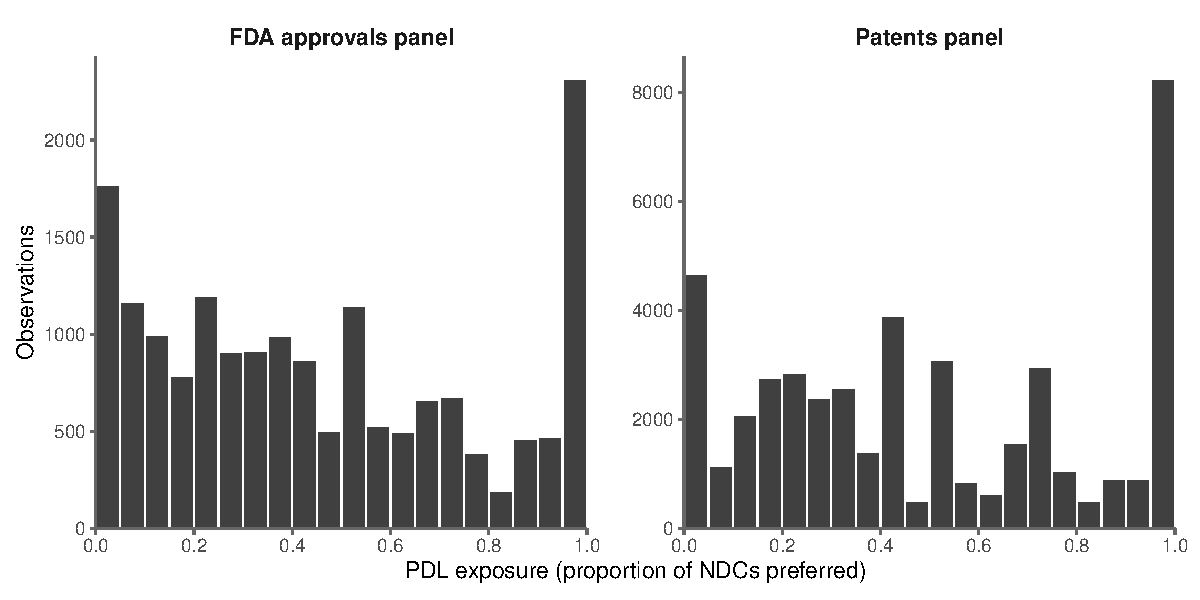
\includegraphics[width=\linewidth]{../output/summary_statistics/pdl_exposure_histogram.pdf}
  \caption{Distribution of PDL exposure in constructed panels}
  \label{fig:pdl_histogram}
\end{figure}

\clearpage

% --- From empirical_results.tex ---

\renewenvironment{table}[1][]{}{}

\subsection{Regression Tables}

\subsubsection{RQ1: Overall Innovation Response}

%TC:ignore
\footnotesize
\begin{table}
\centering
\begin{talltblr}[         %% tabularray outer open
entry=none,label=none,
note{}={* p \num{< 0.05}, ** p \num{< 0.01}, *** p \num{< 0.001}},
]                     %% tabularray outer close
{                     %% tabularray inner open
width=\linewidth,
colspec={Q[]X[]X[]},
column{2,3}={}{halign=c,},
column{1}={}{halign=l,},
hline{32}={1,2,3}{solid, black, 0.05em},
}                     %% tabularray inner close
\toprule
& Patents & FDA Approvals \\ \midrule
2010 × Medicaid Share & \num{-0.041}    & \num{0.215}   \\
                      & (\num{0.038})   & (\num{0.463}) \\
2011 × Medicaid Share & \num{-0.017}    & \num{-0.017}  \\
                      & (\num{0.036})   & (\num{0.381}) \\
2012 × Medicaid Share & \num{0.002}     & \num{0.208}   \\
                      & (\num{0.029})   & (\num{0.412}) \\
2014 × Medicaid Share & \num{-0.022}    & \num{-0.321}  \\
                      & (\num{0.027})   & (\num{0.463}) \\
2015 × Medicaid Share & \num{-0.086}**  & \num{-0.053}  \\
                      & (\num{0.030})   & (\num{0.477}) \\
2016 × Medicaid Share & \num{-0.125}*** & \num{0.414}   \\
                      & (\num{0.034})   & (\num{0.423}) \\
2017 × Medicaid Share & \num{-0.114}**  & \num{1.421}*  \\
                      & (\num{0.036})   & (\num{0.677}) \\
2018 × Medicaid Share & \num{-0.132}*** & \num{0.999}   \\
                      & (\num{0.039})   & (\num{0.550}) \\
2019 × Medicaid Share & \num{-0.189}*** & \num{0.554}   \\
                      & (\num{0.041})   & (\num{0.538}) \\
2020 × Medicaid Share & \num{-0.220}*** & \num{0.732}   \\
                      & (\num{0.043})   & (\num{0.509}) \\
2021 × Medicaid Share & \num{-0.220}*** & \num{0.137}   \\
                      & (\num{0.043})   & (\num{0.632}) \\
2022 × Medicaid Share & \num{-0.233}*** & \num{0.365}   \\
                      & (\num{0.043})   & (\num{0.645}) \\
2023 × Medicaid Share & \num{-0.243}*** & \num{0.846}   \\
                      & (\num{0.044})   & (\num{0.641}) \\
2024 × Medicaid Share & \num{-0.252}*** & \num{0.258}   \\
                      & (\num{0.046})   & (\num{0.523}) \\
2025 × Medicaid Share & \num{-0.228}*** & \num{-0.137}  \\
                      & (\num{0.044})   & (\num{0.510}) \\
Num. obs.             & \num{5281696}   & \num{151200}  \\
R2                    & \num{0.534}     & \num{0.609}   \\
\bottomrule
\end{talltblr}
\end{table}

\captionof{table}{FEOLS event-study estimates: overall innovation response (ex-ante)}
\label{tab:rq1_feols_exante}
\normalsize
%TC:endignore

\clearpage

\subsubsection{RQ2: Medicaid Demand and PDL Exposure}

%TC:ignore
\footnotesize
\begin{table}
\centering
\begin{talltblr}[         %% tabularray outer open
entry=none,label=none,
note{}={* p \num{< 0.05}, ** p \num{< 0.01}, *** p \num{< 0.001}},
]                     %% tabularray outer close
{                     %% tabularray inner open
colspec={Q[]Q[]Q[]Q[]Q[]},
column{2,3,4,5}={}{halign=c,},
column{1}={}{halign=l,},
hline{33}={1,2,3,4,5}{solid, black, 0.05em},
}                     %% tabularray inner close
\toprule
& \SetCell[c=2]{c} Patents && \SetCell[c=2]{c} FDA Approvals & \\
& Medicaid Market Share & PDL Exposure & Medicaid Market Share & PDL Exposure \\ \midrule
2010 & \num{-0.041}    & \num{1.546}     & \num{0.214}   & \num{0.049}   \\
     & (\num{0.038})   & (\num{2.018})   & (\num{0.461}) & (\num{0.807}) \\
2011 & \num{-0.017}    & \num{0.734}     & \num{-0.010}  & \num{-0.243}  \\
     & (\num{0.036})   & (\num{1.642})   & (\num{0.382}) & (\num{0.712}) \\
2012 & \num{0.002}     & \num{1.079}     & \num{0.171}   & \num{1.402}   \\
     & (\num{0.029})   & (\num{1.289})   & (\num{0.406}) & (\num{0.911}) \\
2014 & \num{-0.022}    & \num{4.161}*    & \num{-0.333}  & \num{0.403}   \\
     & (\num{0.026})   & (\num{1.890})   & (\num{0.465}) & (\num{0.647}) \\
2015 & \num{-0.086}**  & \num{0.836}     & \num{-0.088}  & \num{1.163}   \\
     & (\num{0.030})   & (\num{1.480})   & (\num{0.478}) & (\num{0.881}) \\
2016 & \num{-0.126}*** & \num{-1.554}    & \num{0.334}   & \num{2.645}   \\
     & (\num{0.034})   & (\num{1.620})   & (\num{0.426}) & (\num{1.683}) \\
2017 & \num{-0.114}**  & \num{-1.342}    & \num{1.364}*  & \num{1.923}   \\
     & (\num{0.036})   & (\num{1.890})   & (\num{0.680}) & (\num{0.994}) \\
2018 & \num{-0.132}*** & \num{-2.786}    & \num{0.949}   & \num{1.684}   \\
     & (\num{0.039})   & (\num{1.644})   & (\num{0.552}) & (\num{1.021}) \\
2019 & \num{-0.189}*** & \num{-3.806}*   & \num{0.519}   & \num{1.164}*  \\
     & (\num{0.041})   & (\num{1.912})   & (\num{0.539}) & (\num{0.592}) \\
2020 & \num{-0.220}*** & \num{-4.649}*   & \num{0.687}   & \num{1.579}   \\
     & (\num{0.043})   & (\num{1.894})   & (\num{0.514}) & (\num{0.942}) \\
2021 & \num{-0.220}*** & \num{-5.266}**  & \num{0.038}   & \num{3.114}*  \\
     & (\num{0.043})   & (\num{1.687})   & (\num{0.640}) & (\num{1.394}) \\
2022 & \num{-0.233}*** & \num{-6.029}**  & \num{0.333}   & \num{0.994}   \\
     & (\num{0.044})   & (\num{1.941})   & (\num{0.648}) & (\num{0.655}) \\
2023 & \num{-0.243}*** & \num{-6.925}*** & \num{0.809}   & \num{1.185}   \\
     & (\num{0.044})   & (\num{1.851})   & (\num{0.649}) & (\num{1.738}) \\
2024 & \num{-0.252}*** & \num{-6.484}*** & \num{0.272}   & \num{-0.452}  \\
     & (\num{0.046})   & (\num{1.788})   & (\num{0.523}) & (\num{0.590}) \\
2025 & \num{-0.227}*** & \num{-4.588}**  & \num{-0.109}  & \num{-1.118}  \\
     & (\num{0.044})   & (\num{1.549})   & (\num{0.506}) & (\num{0.908}) \\
Num. obs. & \SetCell[c=2]{c} \num{5281696} && \SetCell[c=2]{c} \num{151200} & \\
R2        & \SetCell[c=2]{c} \num{0.535}   && \SetCell[c=2]{c} \num{0.609}  & \\
\bottomrule
\end{talltblr}
\end{table}

\captionof{table}{FEOLS event-study estimates: Medicaid demand and PDL exposure (ex-ante)}
\label{tab:rq2_feols_exante}
\normalsize
%TC:endignore

\clearpage

\subsection{Therapeutic-Class Substitutability}

%TC:ignore
\makeatletter
\renewenvironment{table}[1][H]{\@float{table}[H]}{\end@float}
\makeatother
\begin{table}[!h]
\centering
\caption{\label{tab:class_substitutability}Average annual distinct NDC count by ATC class}
\centering
\begin{tabular}[t]{llr}
\toprule
ATC & Therapeutic class & Mean annual $n_c$\\
\midrule
N & Nervous system & 7351\\
C & Cardiovascular system & 4297\\
A & Alimentary tract and metabolism & 3407\\
J & Anti-infectives for systemic use & 2332\\
D & Dermatologicals & 1771\\
\addlinespace
R & Respiratory system & 1672\\
M & Musculo-skeletal system & 1407\\
B & Blood and blood-forming organs & 1389\\
L & Antineoplastic and immunomodulating & 932\\
G & Genito-urinary and sex hormones & 906\\
\addlinespace
H & Systemic hormonal preparations & 768\\
S & Sensory organs & 579\\
V & Various & 211\\
P & Antiparasitic products & 165\\
\bottomrule
\end{tabular}
\end{table}

\renewenvironment{table}[1][]{}{}
%TC:endignore

\clearpage

% --- From robustness.tex ---

\subsection{Robustness Regression Tables}

\subsubsection{RQ1: Ex-Post FEOLS}

%TC:ignore
\footnotesize
\begin{table}
\centering
\begin{talltblr}[         %% tabularray outer open
entry=none,label=none,
note{}={* p \num{< 0.05}, ** p \num{< 0.01}, *** p \num{< 0.001}},
]                     %% tabularray outer close
{                     %% tabularray inner open
width=\linewidth,
colspec={Q[]X[]X[]},
column{2,3}={}{halign=c,},
column{1}={}{halign=l,},
hline{32}={1,2,3}{solid, black, 0.05em},
}                     %% tabularray inner close
\toprule
& Patents & FDA Approvals \\ \midrule
2010 × Medicaid Share & \num{-0.033}    & \num{0.286}   \\
                      & (\num{0.035})   & (\num{0.450}) \\
2011 × Medicaid Share & \num{-0.010}    & \num{0.336}   \\
                      & (\num{0.033})   & (\num{0.413}) \\
2012 × Medicaid Share & \num{0.004}     & \num{0.414}   \\
                      & (\num{0.027})   & (\num{0.455}) \\
2014 × Medicaid Share & \num{-0.018}    & \num{-0.324}  \\
                      & (\num{0.024})   & (\num{0.533}) \\
2015 × Medicaid Share & \num{-0.088}**  & \num{0.005}   \\
                      & (\num{0.027})   & (\num{0.420}) \\
2016 × Medicaid Share & \num{-0.123}*** & \num{0.550}   \\
                      & (\num{0.032})   & (\num{0.413}) \\
2017 × Medicaid Share & \num{-0.122}*** & \num{1.635}*  \\
                      & (\num{0.034})   & (\num{0.688}) \\
2018 × Medicaid Share & \num{-0.135}*** & \num{1.240}*  \\
                      & (\num{0.037})   & (\num{0.560}) \\
2019 × Medicaid Share & \num{-0.194}*** & \num{0.400}   \\
                      & (\num{0.039})   & (\num{0.497}) \\
2020 × Medicaid Share & \num{-0.225}*** & \num{0.652}   \\
                      & (\num{0.041})   & (\num{0.529}) \\
2021 × Medicaid Share & \num{-0.222}*** & \num{0.218}   \\
                      & (\num{0.040})   & (\num{0.573}) \\
2022 × Medicaid Share & \num{-0.233}*** & \num{0.418}   \\
                      & (\num{0.040})   & (\num{0.590}) \\
2023 × Medicaid Share & \num{-0.238}*** & \num{0.842}   \\
                      & (\num{0.040})   & (\num{0.576}) \\
2024 × Medicaid Share & \num{-0.250}*** & \num{0.137}   \\
                      & (\num{0.042})   & (\num{0.502}) \\
2025 × Medicaid Share & \num{-0.212}*** & \num{-0.380}  \\
                      & (\num{0.041})   & (\num{0.531}) \\
Num. obs.             & \num{5281696}   & \num{151200}  \\
R2                    & \num{0.534}     & \num{0.609}   \\
\bottomrule
\end{talltblr}
\end{table}

\captionof{table}{FEOLS event-study estimates: overall innovation response (ex-post)}
\label{tab:rob_rq1_feols_expost}
\normalsize
%TC:endignore

\begin{figure}[!h]
  \centering
  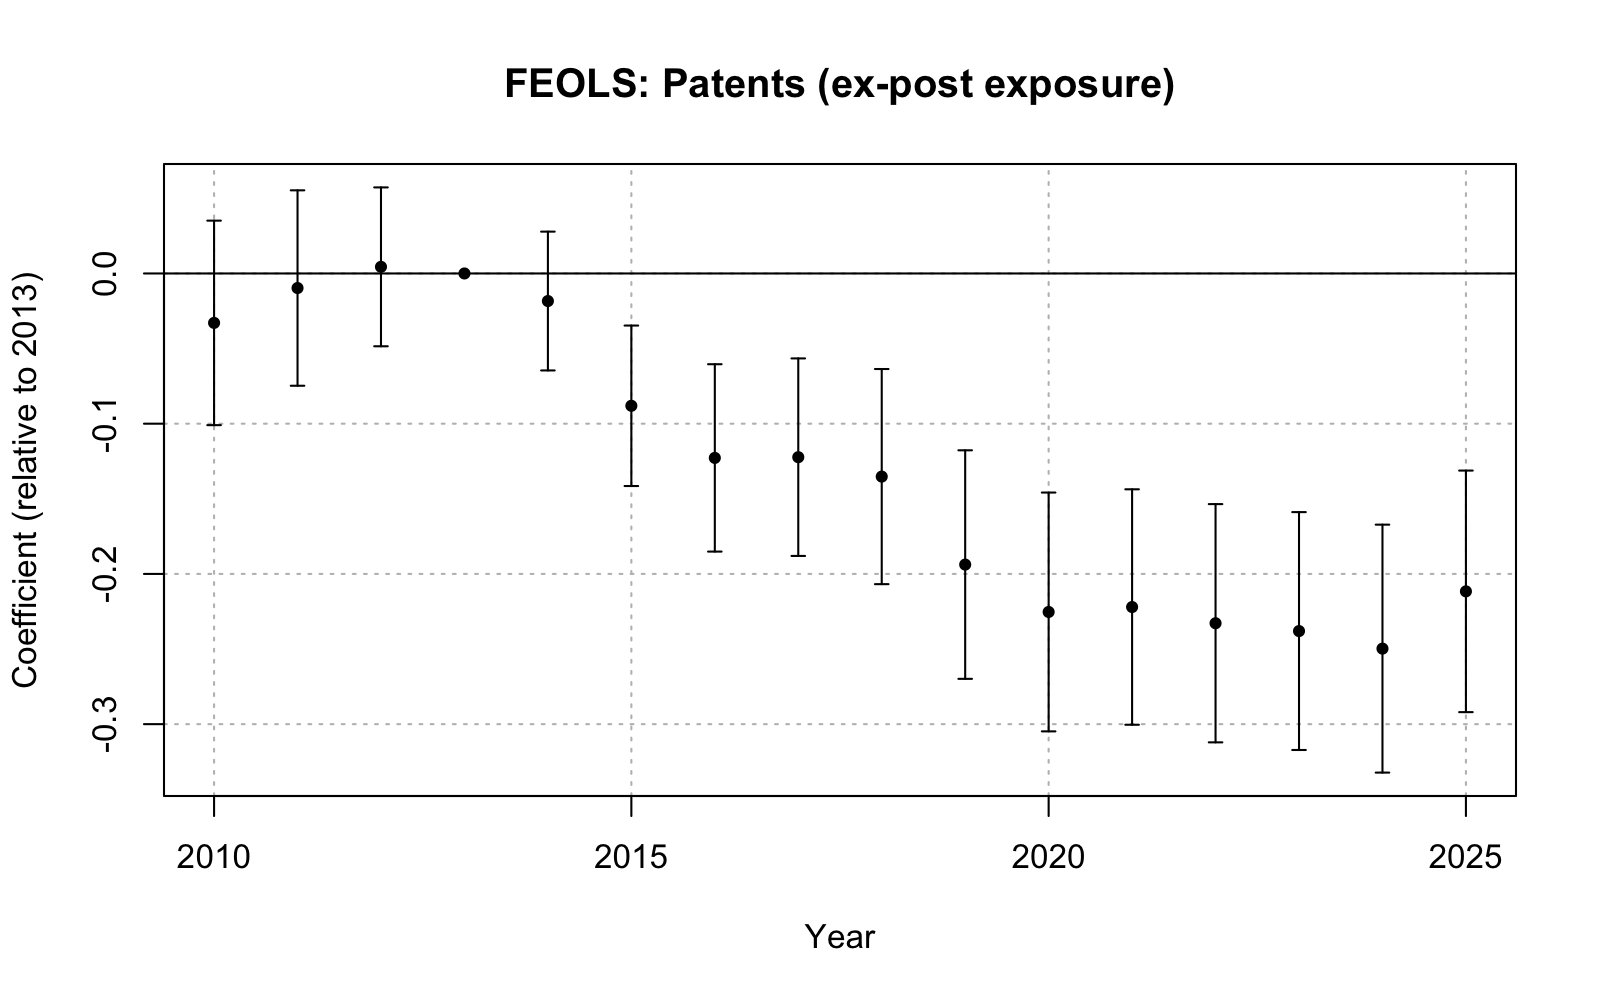
\includegraphics[width=\linewidth]{../output/RQ1/patent_feols_expost.png}
  \caption{FEOLS event study: patents, ex-post Medicaid exposure}
  \label{fig:rob_rq1_patent_feols_expost}
\end{figure}

\begin{figure}[!h]
  \centering
  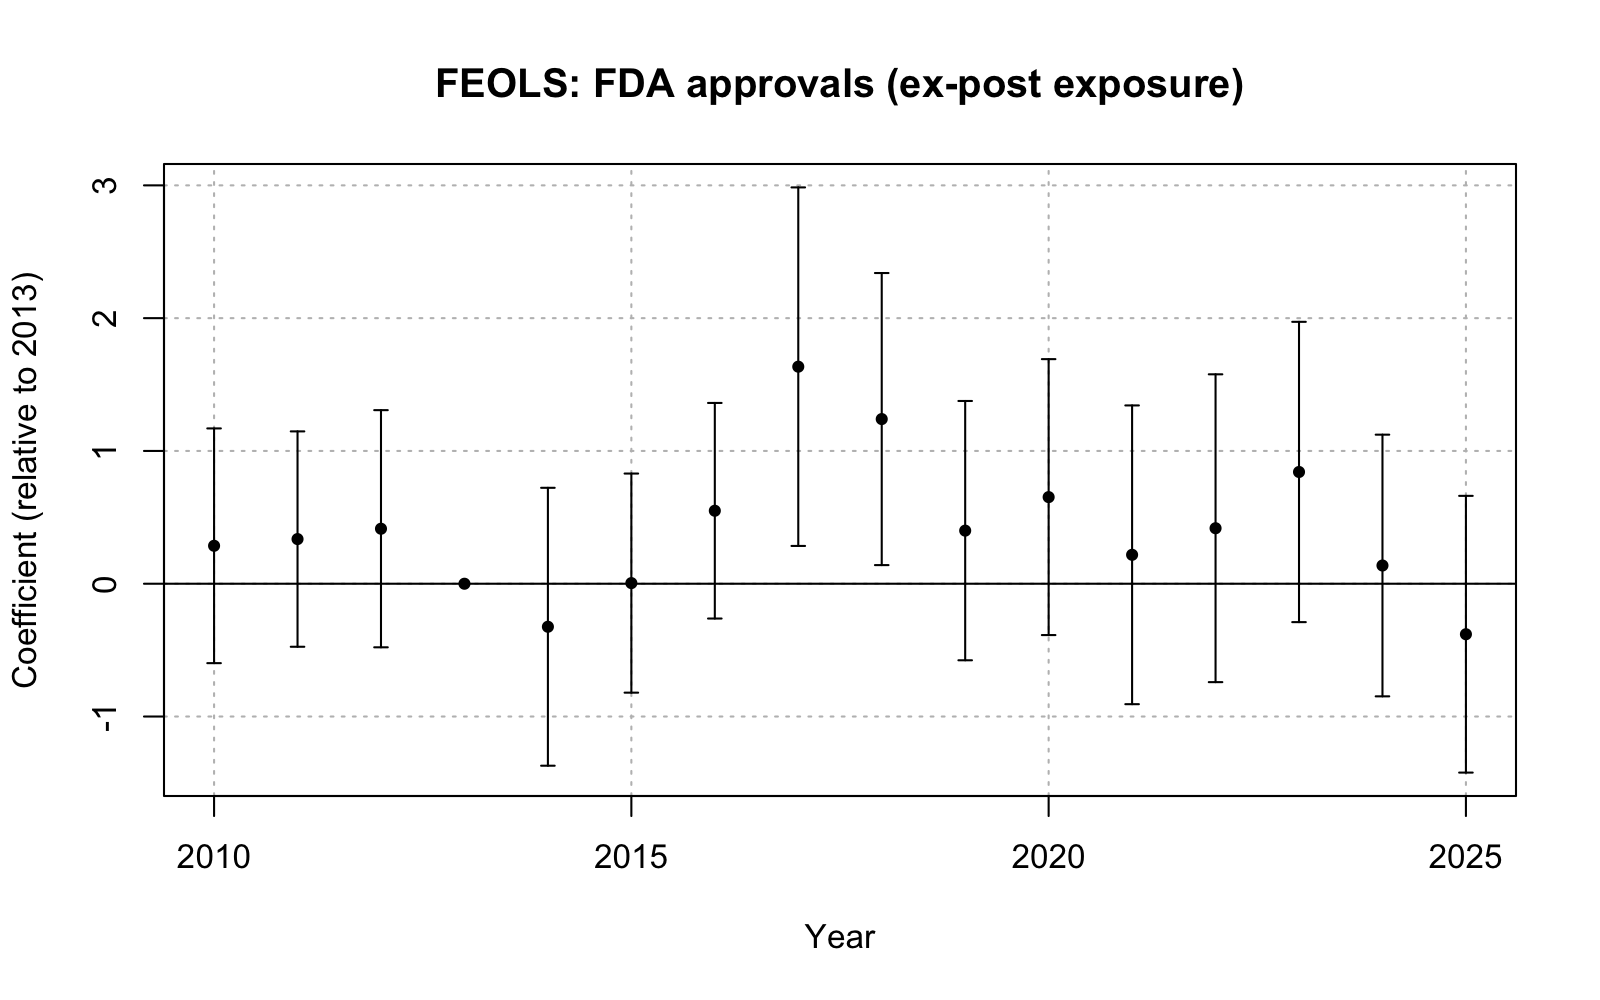
\includegraphics[width=\linewidth]{../output/RQ1/fda_feols_expost.png}
  \caption{FEOLS event study: FDA approvals, ex-post Medicaid exposure}
  \label{fig:rob_rq1_fda_feols_expost}
\end{figure}

\clearpage

\subsubsection{RQ1: Ex-Ante FE Poisson}

%TC:ignore
\footnotesize
\begin{table}
\centering
\begin{talltblr}[         %% tabularray outer open
entry=none,label=none,
note{}={* p \num{< 0.05}, ** p \num{< 0.01}, *** p \num{< 0.001}},
]                     %% tabularray outer close
{                     %% tabularray inner open
width=\linewidth,
colspec={Q[]X[]X[]},
column{2,3}={}{halign=c,},
column{1}={}{halign=l,},
hline{32}={1,2,3}{solid, black, 0.05em},
}                     %% tabularray inner close
\toprule
& Patents & FDA Approvals \\ \midrule
2010 × Medicaid Share & \num{0.120}     & \num{0.237}   \\
                      & (\num{0.154})   & (\num{0.636}) \\
2011 × Medicaid Share & \num{0.218}     & \num{0.326}   \\
                      & (\num{0.140})   & (\num{0.446}) \\
2012 × Medicaid Share & \num{0.115}     & \num{0.643}   \\
                      & (\num{0.108})   & (\num{0.615}) \\
2014 × Medicaid Share & \num{-0.092}    & \num{-0.545}  \\
                      & (\num{0.108})   & (\num{0.638}) \\
2015 × Medicaid Share & \num{-0.300}*   & \num{-0.434}  \\
                      & (\num{0.118})   & (\num{0.632}) \\
2016 × Medicaid Share & \num{-0.435}*** & \num{-0.834}  \\
                      & (\num{0.124})   & (\num{0.478}) \\
2017 × Medicaid Share & \num{-0.397}**  & \num{-0.495}  \\
                      & (\num{0.131})   & (\num{0.480}) \\
2018 × Medicaid Share & \num{-0.415}**  & \num{-0.772}  \\
                      & (\num{0.149})   & (\num{0.530}) \\
2019 × Medicaid Share & \num{-0.784}*** & \num{-0.381}  \\
                      & (\num{0.154})   & (\num{0.565}) \\
2020 × Medicaid Share & \num{-0.998}*** & \num{-0.733}  \\
                      & (\num{0.173})   & (\num{0.574}) \\
2021 × Medicaid Share & \num{-0.989}*** & \num{-0.867}  \\
                      & (\num{0.170})   & (\num{0.729}) \\
2022 × Medicaid Share & \num{-1.137}*** & \num{-0.637}  \\
                      & (\num{0.186})   & (\num{0.594}) \\
2023 × Medicaid Share & \num{-1.324}*** & \num{-0.566}  \\
                      & (\num{0.201})   & (\num{0.511}) \\
2024 × Medicaid Share & \num{-1.474}*** & \num{-0.680}  \\
                      & (\num{0.261})   & (\num{0.573}) \\
2025 × Medicaid Share & \num{-1.110}*** & \num{-0.668}  \\
                      & (\num{0.229})   & (\num{0.580}) \\
Num. obs.             & \num{1300944}   & \num{42176}   \\
\bottomrule
\end{talltblr}
\end{table}

\captionof{table}{FE Poisson event-study estimates: overall innovation response (ex-ante)}
\label{tab:rob_rq1_fepois_exante}
\normalsize
%TC:endignore

\begin{figure}[!h]
  \centering
  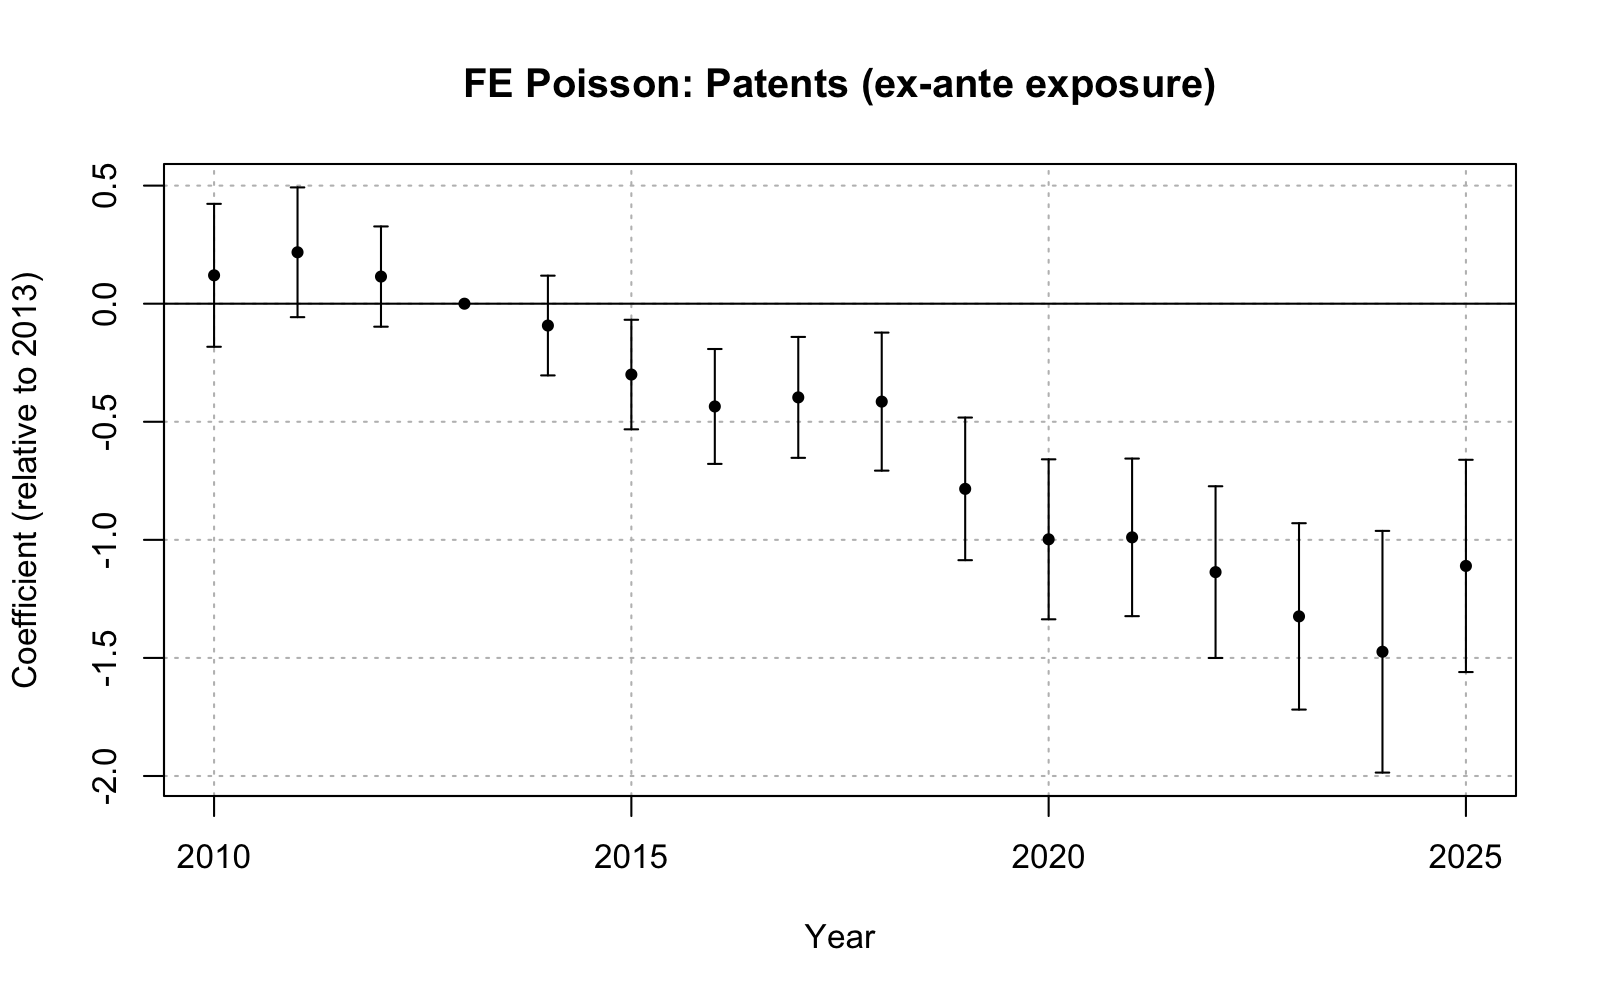
\includegraphics[width=\linewidth]{../output/RQ1/patent_poi_exante.png}
  \caption{FE Poisson event study: patents, ex-ante Medicaid exposure}
  \label{fig:rob_rq1_patent_poi_exante}
\end{figure}

\begin{figure}[!h]
  \centering
  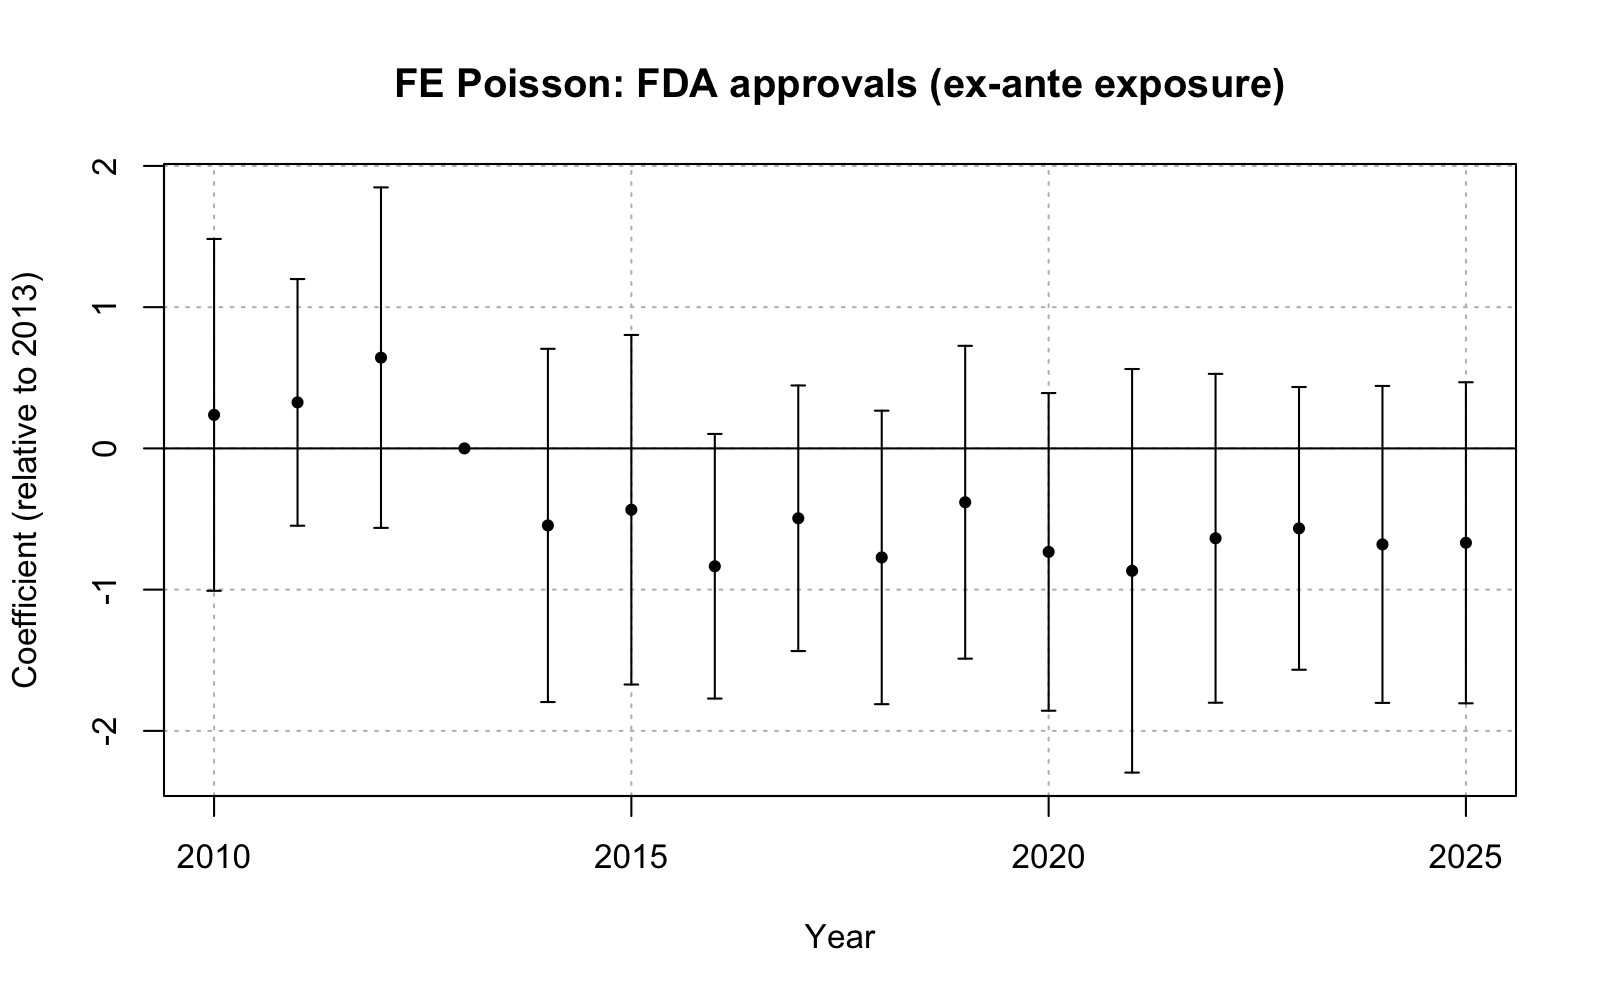
\includegraphics[width=\linewidth]{../output/RQ1/fda_poi_exante.png}
  \caption{FE Poisson event study: FDA approvals, ex-ante Medicaid exposure}
  \label{fig:rob_rq1_fda_poi_exante}
\end{figure}

\clearpage

\subsubsection{RQ1: Ex-Post FE Poisson}

%TC:ignore
\footnotesize
\begin{table}
\centering
\begin{talltblr}[         %% tabularray outer open
entry=none,label=none,
note{}={* p \num{< 0.05}, ** p \num{< 0.01}, *** p \num{< 0.001}},
]                     %% tabularray outer close
{                     %% tabularray inner open
width=\linewidth,
colspec={Q[]X[]X[]},
column{2,3}={}{halign=c,},
column{1}={}{halign=l,},
hline{32}={1,2,3}{solid, black, 0.05em},
}                     %% tabularray inner close
\toprule
& Patents & FDA Approvals \\ \midrule
2010 × Medicaid Share & \num{0.129}     & \num{0.453}   \\
                      & (\num{0.157})   & (\num{0.869}) \\
2011 × Medicaid Share & \num{0.240}     & \num{1.138}   \\
                      & (\num{0.145})   & (\num{0.687}) \\
2012 × Medicaid Share & \num{0.124}     & \num{1.250}   \\
                      & (\num{0.115})   & (\num{0.863}) \\
2014 × Medicaid Share & \num{-0.086}    & \num{-0.711}  \\
                      & (\num{0.106})   & (\num{0.996}) \\
2015 × Medicaid Share & \num{-0.367}**  & \num{-0.431}  \\
                      & (\num{0.119})   & (\num{0.725}) \\
2016 × Medicaid Share & \num{-0.515}*** & \num{-0.788}  \\
                      & (\num{0.129})   & (\num{0.660}) \\
2017 × Medicaid Share & \num{-0.533}*** & \num{-0.278}  \\
                      & (\num{0.134})   & (\num{0.735}) \\
2018 × Medicaid Share & \num{-0.556}*** & \num{-0.595}  \\
                      & (\num{0.157})   & (\num{0.713}) \\
2019 × Medicaid Share & \num{-0.998}*** & \num{-0.625}  \\
                      & (\num{0.167})   & (\num{0.764}) \\
2020 × Medicaid Share & \num{-1.293}*** & \num{-0.916}  \\
                      & (\num{0.190})   & (\num{0.839}) \\
2021 × Medicaid Share & \num{-1.313}*** & \num{-0.909}  \\
                      & (\num{0.188})   & (\num{0.910}) \\
2022 × Medicaid Share & \num{-1.564}*** & \num{-0.657}  \\
                      & (\num{0.203})   & (\num{0.775}) \\
2023 × Medicaid Share & \num{-1.803}*** & \num{-0.618}  \\
                      & (\num{0.224})   & (\num{0.695}) \\
2024 × Medicaid Share & \num{-2.021}*** & \num{-0.969}  \\
                      & (\num{0.266})   & (\num{0.854}) \\
2025 × Medicaid Share & \num{-1.692}*** & \num{-1.254}  \\
                      & (\num{0.262})   & (\num{0.892}) \\
Num. obs.             & \num{1300944}   & \num{42176}   \\
\bottomrule
\end{talltblr}
\end{table}

\captionof{table}{FE Poisson event-study estimates: overall innovation response (ex-post)}
\label{tab:rob_rq1_fepois_expost}
\normalsize
%TC:endignore

\begin{figure}[!h]
  \centering
  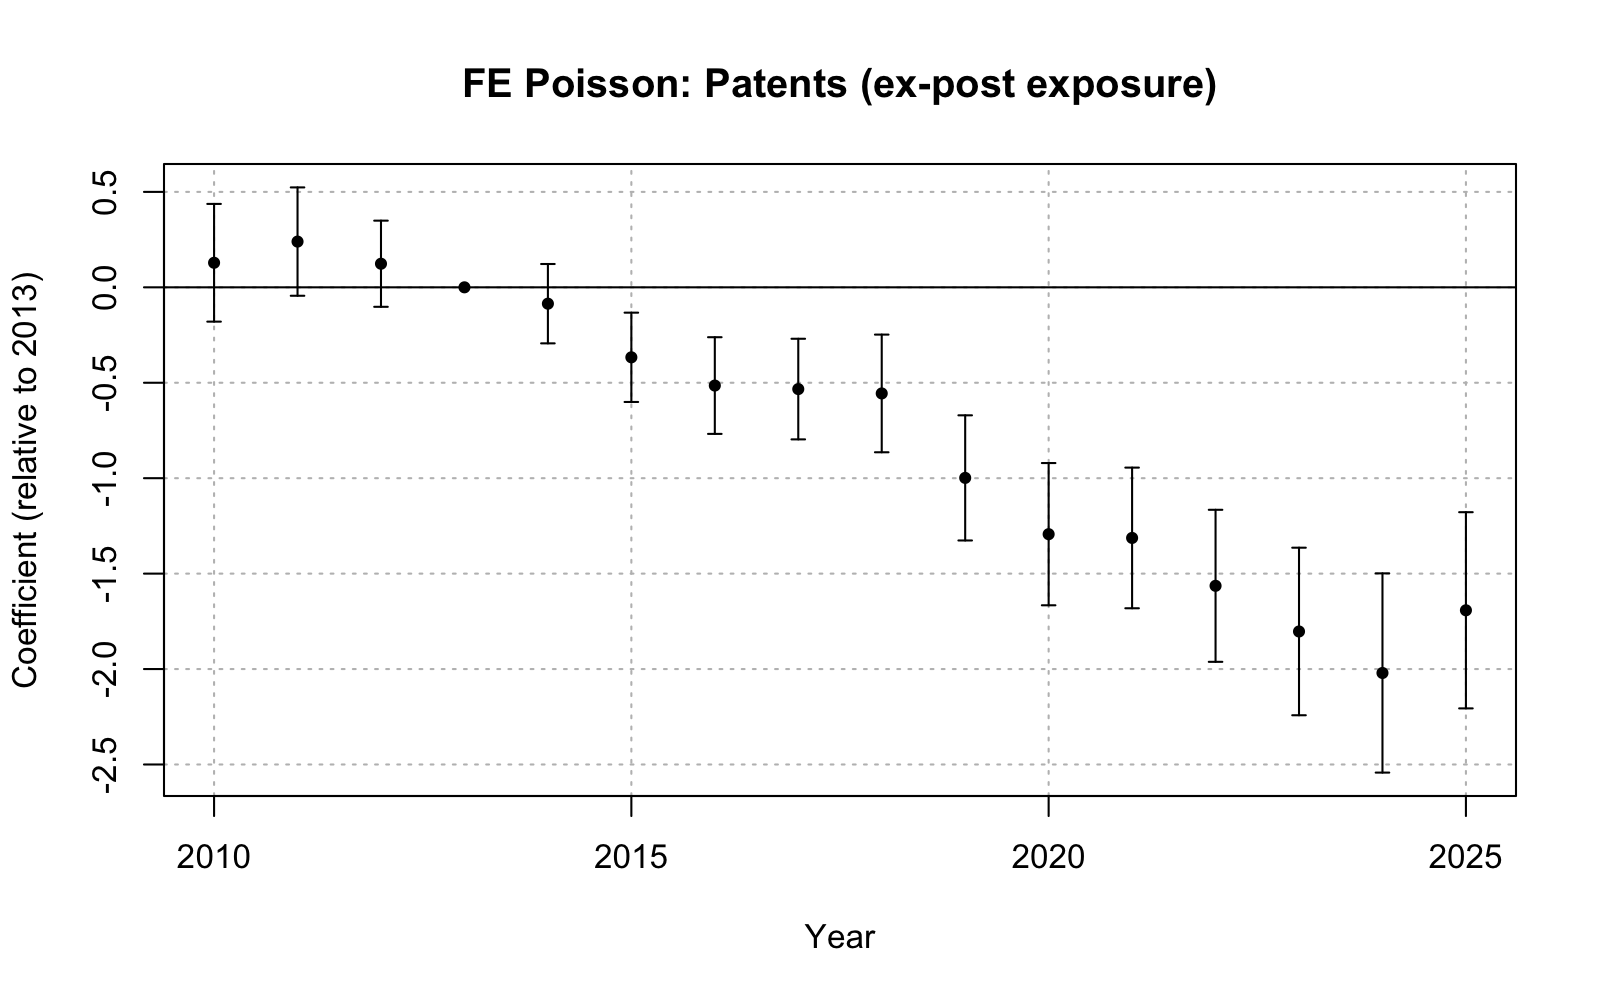
\includegraphics[width=\linewidth]{../output/RQ1/patent_poi_expost.png}
  \caption{FE Poisson event study: patents, ex-post Medicaid exposure}
  \label{fig:rob_rq1_patent_poi_expost}
\end{figure}

\begin{figure}[!h]
  \centering
  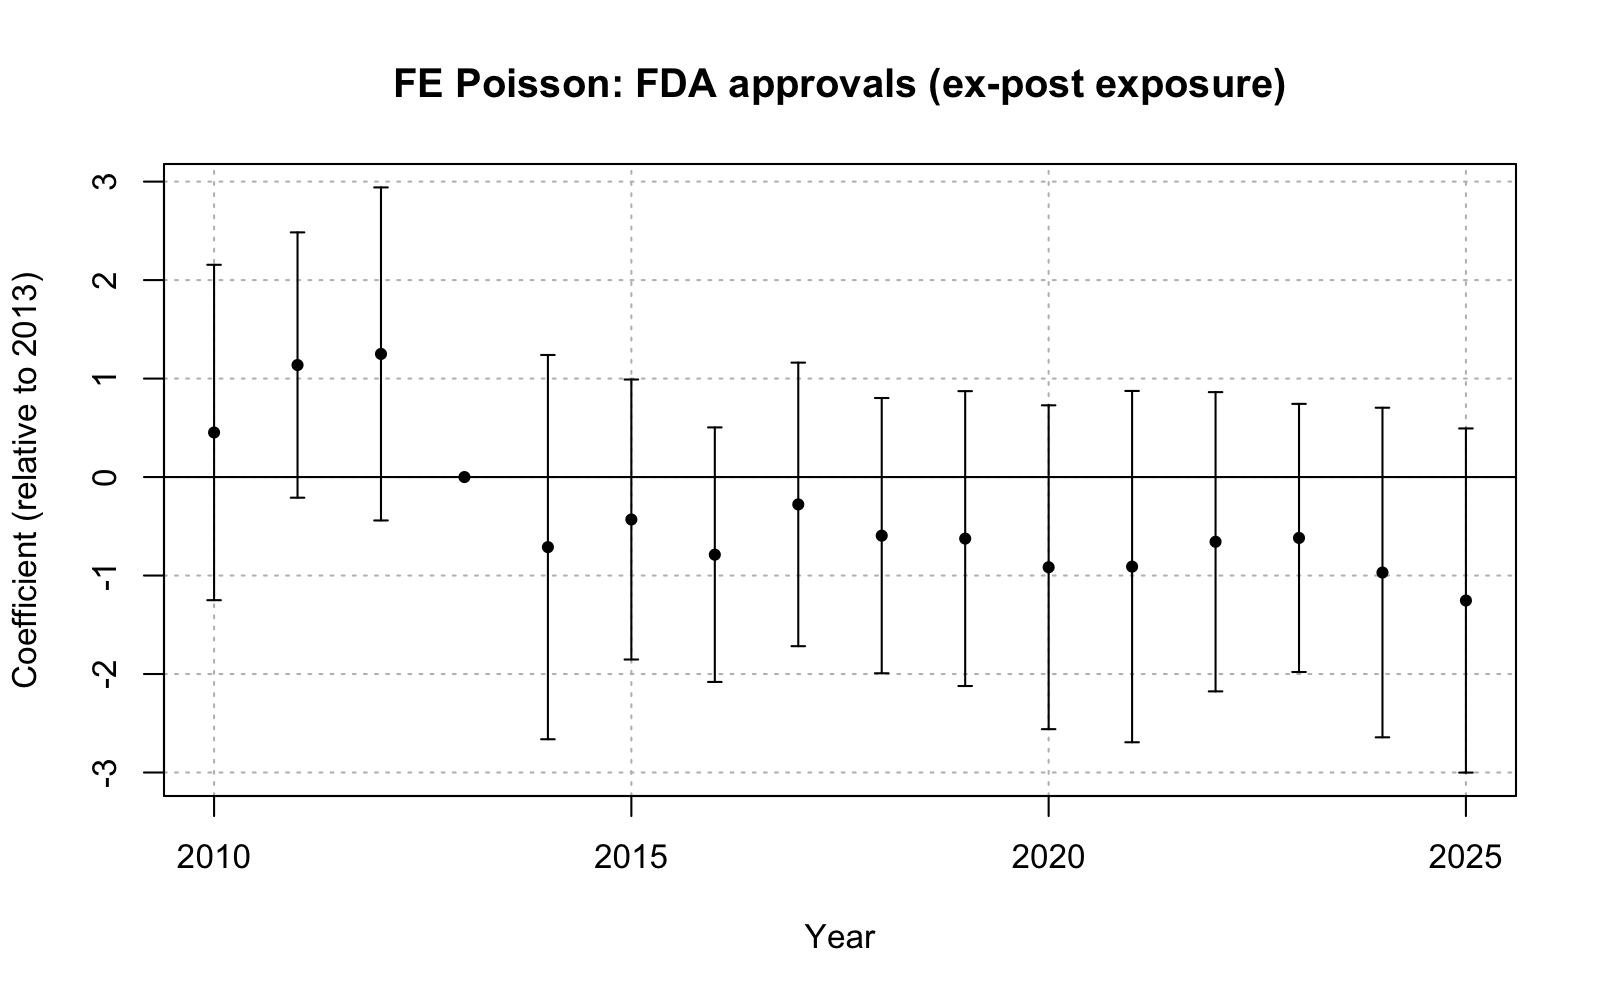
\includegraphics[width=\linewidth]{../output/RQ1/fda_poi_expost.png}
  \caption{FE Poisson event study: FDA approvals, ex-post Medicaid exposure}
  \label{fig:rob_rq1_fda_poi_expost}
\end{figure}

\clearpage

\subsubsection{RQ1: Binned Treatment}

%TC:ignore
\makeatletter
\renewenvironment{table}[1][H]{\@float{table}[H]}{\end@float}
\makeatother
\begin{table}[htbp]
\centering
\caption{Pre-expansion Medicaid market shares and bin assignments}
\label{tab:atc_bins}
\begin{tabular}{llrl}
\toprule
\multicolumn{1}{c}{ATC} & \multicolumn{1}{c}{Therapeutic Area} & \multicolumn{1}{c}{Medicaid Share} & \multicolumn{1}{c}{Bin} \\
\midrule
N & Nervous system                  & 0.363 & High   \\
C & Cardiovascular system           & 0.215 & High   \\
J & Anti-infectives for systemic use & 0.120 & Medium \\
D & Dermatologicals                 & 0.099 & Medium \\
R & Respiratory system              & 0.085 & Low    \\
A & Alimentary tract and metabolism & 0.068 & Low    \\
M & Musculo-skeletal system         & 0.015 & Low    \\
H & Systemic hormonal preparations  & 0.012 & Low    \\
L & Antineoplastic and immunomodulating agents & 0.006 & Low \\
G & Genito-urinary system and sex hormones     & 0.006 & Low \\
S & Sensory organs                  & 0.005 & Low    \\
B & Blood and blood-forming organs  & 0.005 & Low    \\
V & Various                         & 0.000 & Low    \\
P & Antiparasitic products          & 0.000 & Low    \\
\bottomrule
\end{tabular}
\end{table}

\renewenvironment{table}[1][]{}{}
%TC:endignore

%TC:ignore
\footnotesize
\begin{table}
\centering
\begin{talltblr}[         %% tabularray outer open
entry=none,label=none,
note{}={* p \num{< 0.05}, ** p \num{< 0.01}, *** p \num{< 0.001}},
]                     %% tabularray outer close
{                     %% tabularray inner open
width=\linewidth,
colspec={Q[]X[]X[]X[]X[]},
column{2,3,4,5}={}{halign=c,},
column{1}={}{halign=l,},
hline{33}={1,2,3,4,5}{solid, black, 0.05em},
}                     %% tabularray inner close
\toprule
& \SetCell[c=2]{c} Patents && \SetCell[c=2]{c} FDA Approvals & \\
& Medium Bin & High Bin & Medium Bin & High Bin \\ \midrule
2010 & \num{-0.008}    & \num{-0.029}    & \num{0.042}   & \num{0.085}   \\
     & (\num{0.006})   & (\num{0.017})   & (\num{0.055}) & (\num{0.140}) \\
2011 & \num{-0.005}    & \num{-0.025}    & \num{0.058}   & \num{-0.064}  \\
     & (\num{0.006})   & (\num{0.016})   & (\num{0.065}) & (\num{0.105}) \\
2012 & \num{0.009}     & \num{-0.003}    & \num{0.042}   & \num{0.033}   \\
     & (\num{0.006})   & (\num{0.012})   & (\num{0.077}) & (\num{0.121}) \\
2014 & \num{0.015}**   & \num{-0.002}    & \num{0.047}   & \num{-0.091}  \\
     & (\num{0.005})   & (\num{0.011})   & (\num{0.067}) & (\num{0.130}) \\
2015 & \num{0.002}     & \num{-0.027}*   & \num{0.006}   & \num{-0.005}  \\
     & (\num{0.005})   & (\num{0.013})   & (\num{0.073}) & (\num{0.148}) \\
2016 & \num{0.007}     & \num{-0.058}*** & \num{0.158}   & \num{0.070}   \\
     & (\num{0.006})   & (\num{0.014})   & (\num{0.101}) & (\num{0.130}) \\
2017 & \num{0.005}     & \num{-0.047}**  & \num{0.239}*  & \num{0.326}   \\
     & (\num{0.006})   & (\num{0.015})   & (\num{0.114}) & (\num{0.181}) \\
2018 & \num{-0.009}    & \num{-0.075}*** & \num{0.185}*  & \num{0.213}   \\
     & (\num{0.006})   & (\num{0.017})   & (\num{0.093}) & (\num{0.155}) \\
2019 & \num{-0.004}    & \num{-0.092}*** & \num{0.071}   & \num{0.206}   \\
     & (\num{0.007})   & (\num{0.017})   & (\num{0.077}) & (\num{0.162}) \\
2020 & \num{-0.003}    & \num{-0.108}*** & \num{0.012}   & \num{0.141}   \\
     & (\num{0.006})   & (\num{0.018})   & (\num{0.092}) & (\num{0.142}) \\
2021 & \num{-0.005}    & \num{-0.118}*** & \num{0.127}   & \num{-0.048}  \\
     & (\num{0.006})   & (\num{0.018})   & (\num{0.105}) & (\num{0.182}) \\
2022 & \num{-0.010}    & \num{-0.129}*** & \num{0.101}   & \num{0.040}   \\
     & (\num{0.006})   & (\num{0.018})   & (\num{0.075}) & (\num{0.184}) \\
2023 & \num{-0.011}    & \num{-0.141}*** & \num{0.152}   & \num{0.154}   \\
     & (\num{0.006})   & (\num{0.019})   & (\num{0.087}) & (\num{0.182}) \\
2024 & \num{-0.005}    & \num{-0.142}*** & \num{0.037}   & \num{0.070}   \\
     & (\num{0.010})   & (\num{0.019})   & (\num{0.066}) & (\num{0.146}) \\
2025 & \num{-0.020}**  & \num{-0.155}*** & \num{0.010}   & \num{0.032}   \\
     & (\num{0.006})   & (\num{0.019})   & (\num{0.067}) & (\num{0.153}) \\
Num. obs. & \SetCell[c=2]{c} \num{5281696} && \SetCell[c=2]{c} \num{151200} & \\
R2        & \SetCell[c=2]{c} \num{0.534}   && \SetCell[c=2]{c} \num{0.609}  & \\
\bottomrule
\end{talltblr}
\end{table}

\captionof{table}{Binned treatment event-study estimates (FEOLS, ex-ante)}
\label{tab:rob_binned}
\normalsize
%TC:endignore

\begin{figure}[!h]
  \centering
  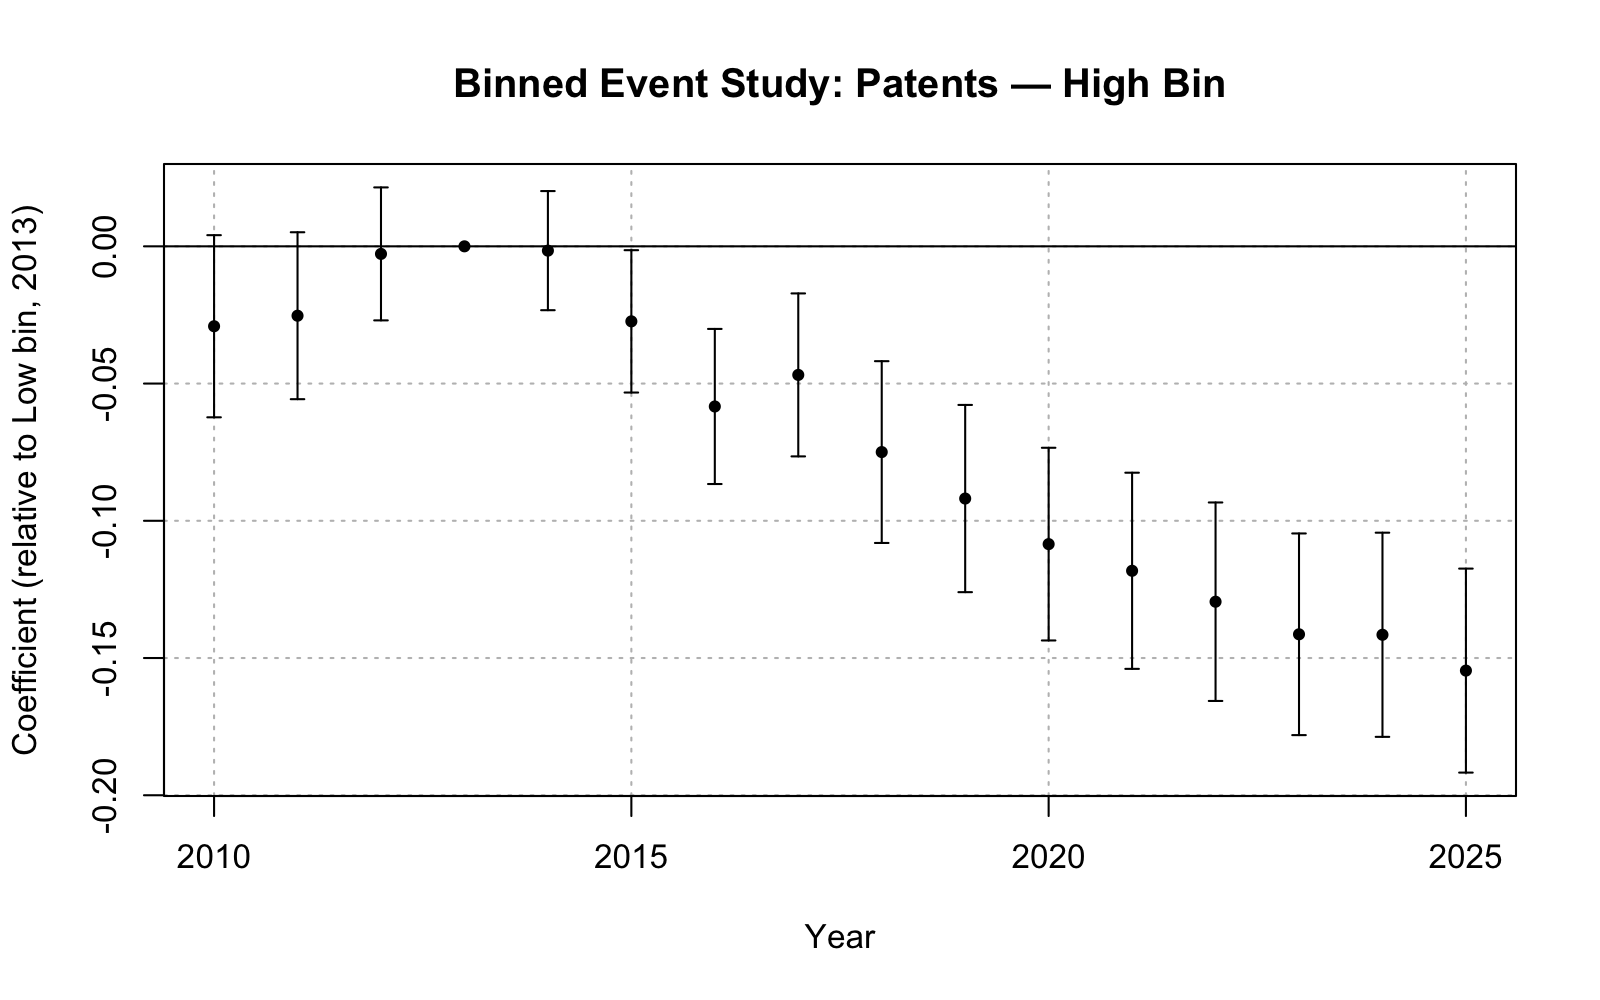
\includegraphics[width=\linewidth]{../output/robustness/binned_treatment/binned_patent_high_es.png}
  \caption{Binned event study: patents, high-exposure bin (N, C)}
  \label{fig:rob_binned_patent_high}
\end{figure}

\begin{figure}[!h]
  \centering
  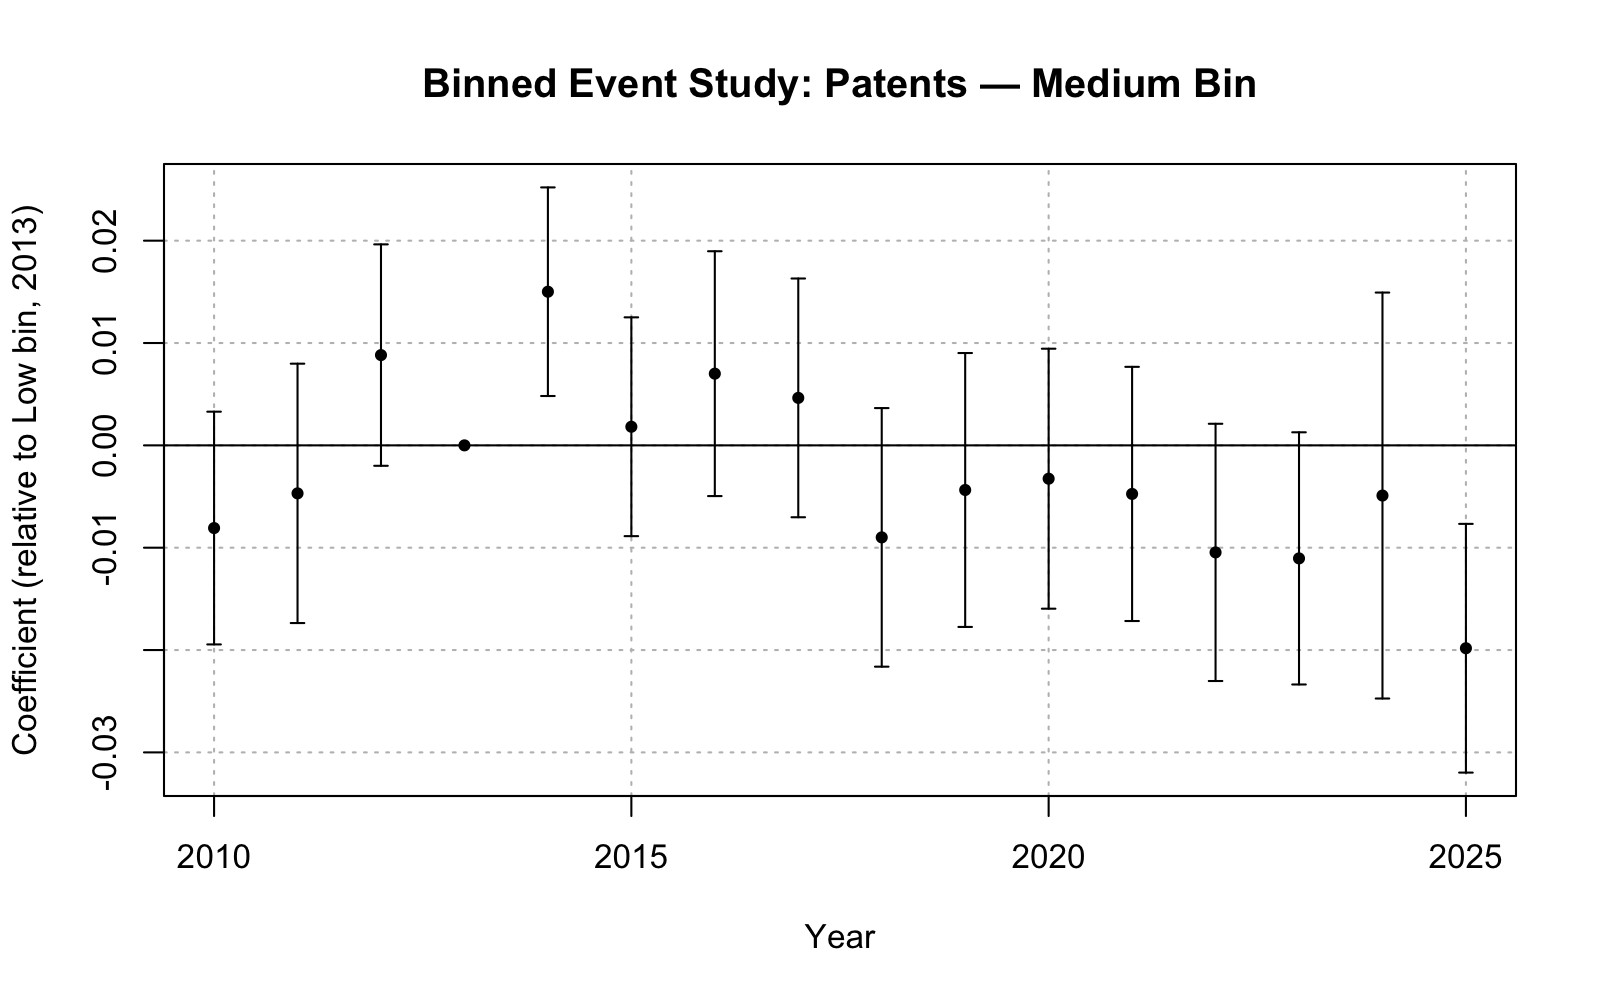
\includegraphics[width=\linewidth]{../output/robustness/binned_treatment/binned_patent_medium_es.png}
  \caption{Binned event study: patents, medium-exposure bin (J, D)}
  \label{fig:rob_binned_patent_medium}
\end{figure}

\clearpage

\begin{figure}[!h]
  \centering
  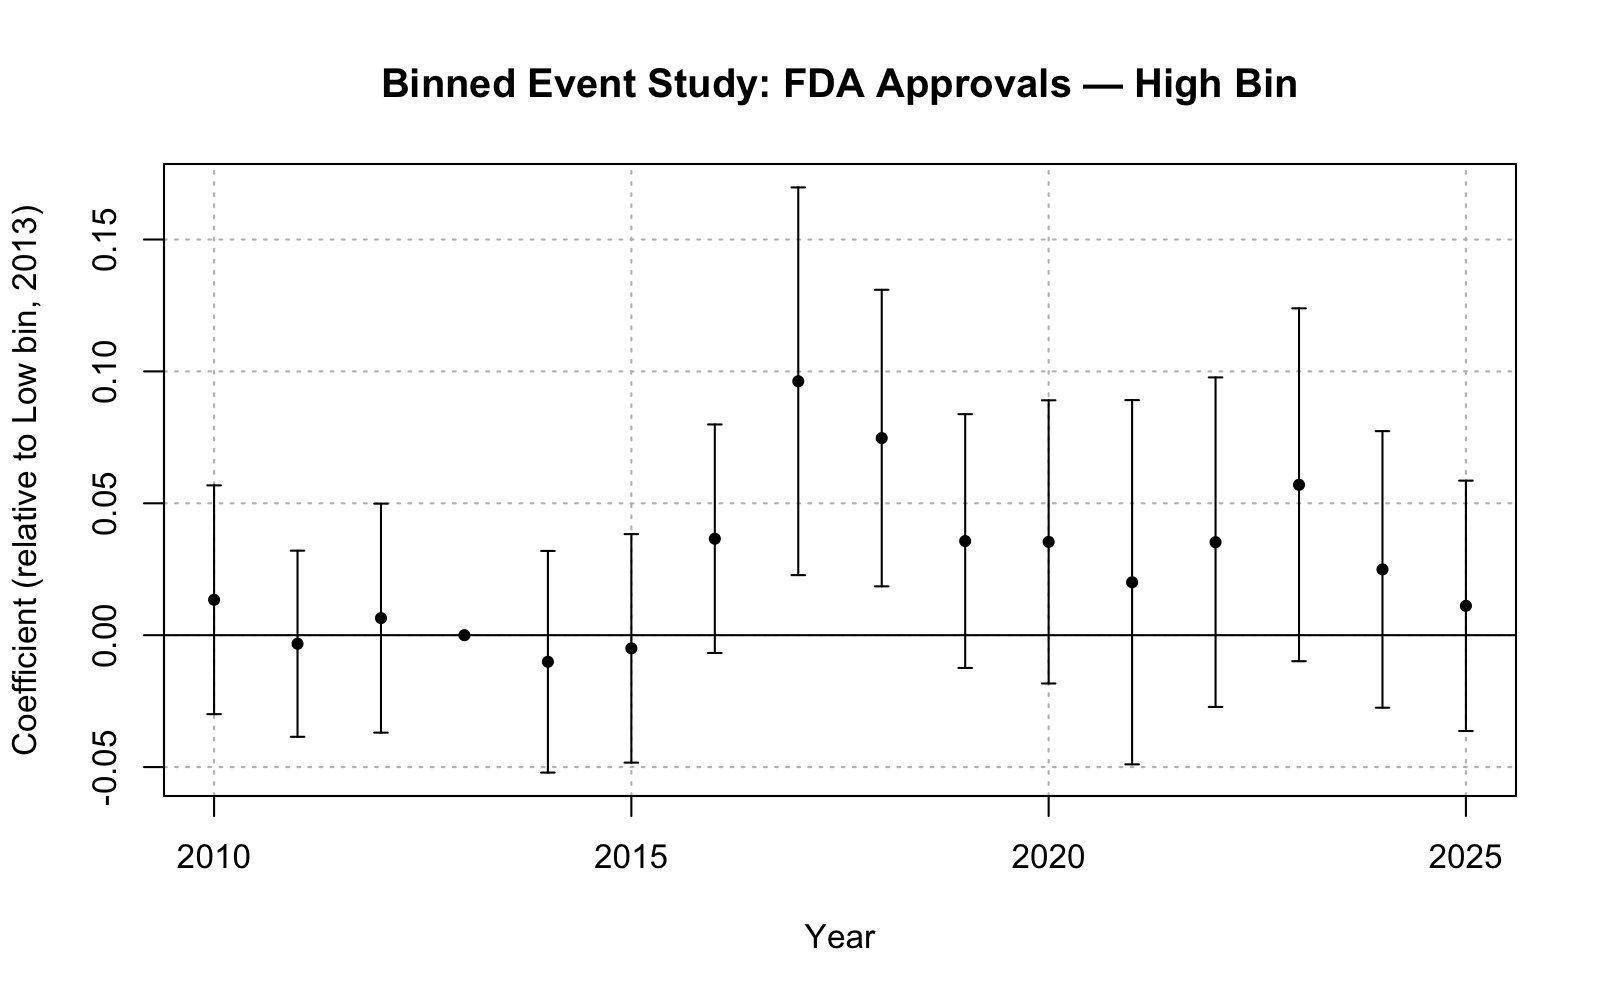
\includegraphics[width=\linewidth]{../output/robustness/binned_treatment/binned_fda_high_es.png}
  \caption{Binned event study: FDA approvals, high-exposure bin (N, C)}
  \label{fig:rob_binned_fda_high}
\end{figure}

\begin{figure}[!h]
  \centering
  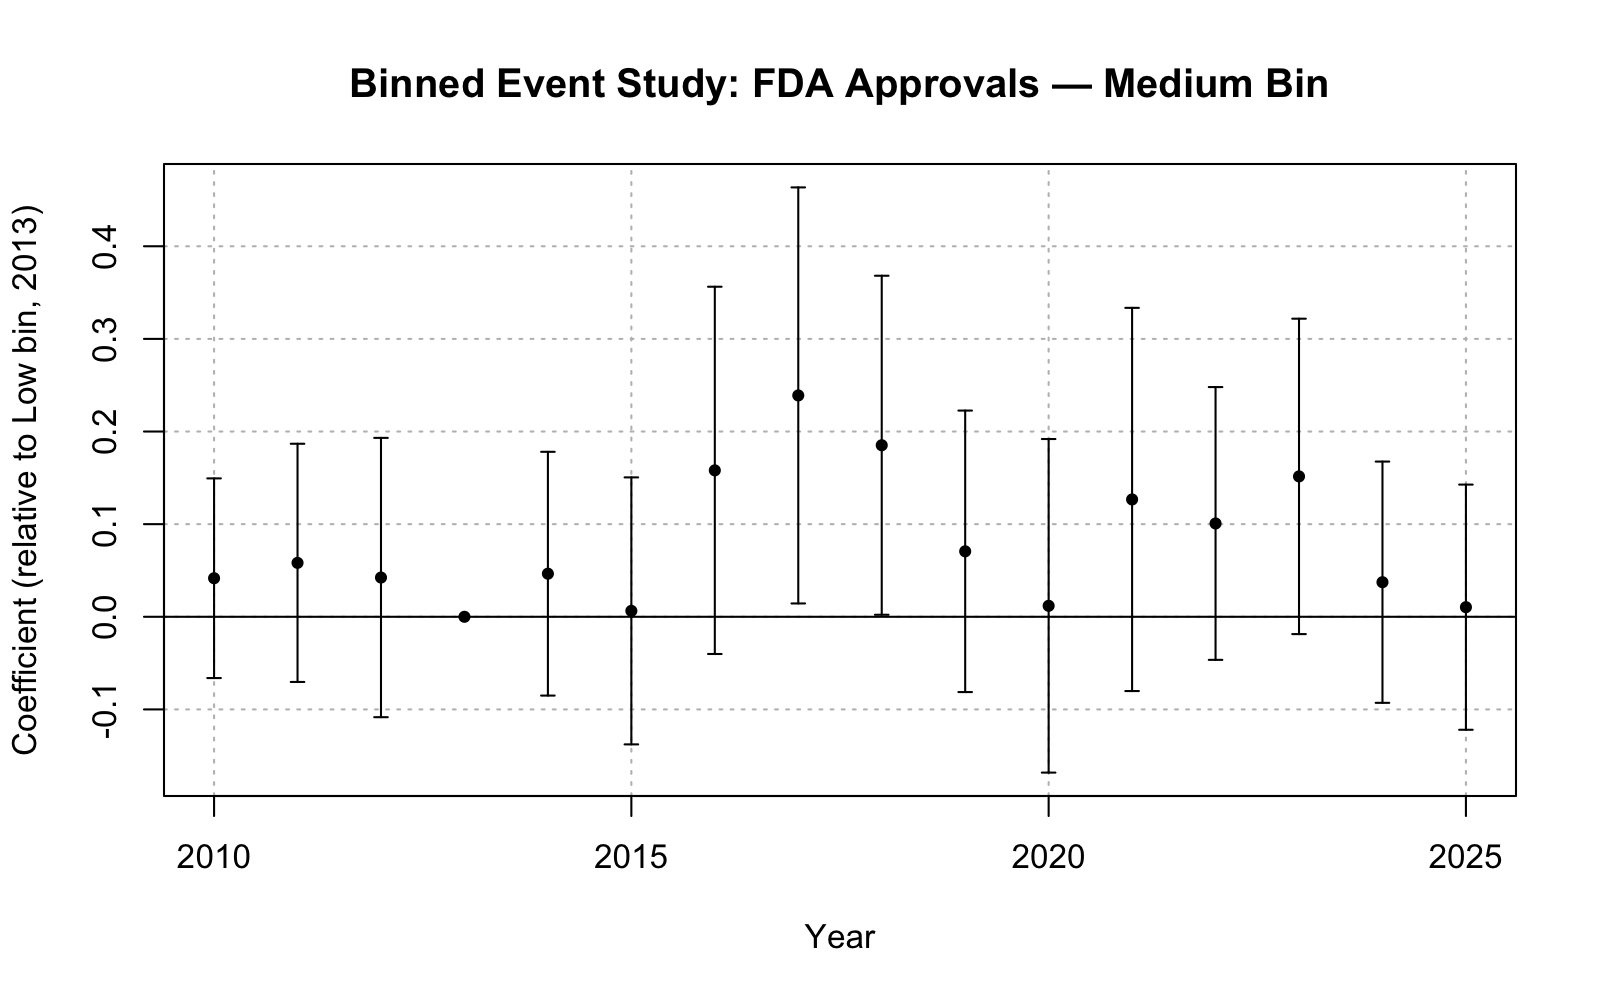
\includegraphics[width=\linewidth]{../output/robustness/binned_treatment/binned_fda_medium_es.png}
  \caption{Binned event study: FDA approvals, medium-exposure bin (J, D)}
  \label{fig:rob_binned_fda_medium}
\end{figure}

\clearpage

\subsubsection{RQ1: Continuous Difference-in-Differences}

%TC:ignore
\makeatletter
\renewenvironment{table}[1][H]{\@float{table}[H]}{\end@float}
\makeatother
\footnotesize
\begin{table}
\centering
\begin{talltblr}[         %% tabularray outer open
entry=none,label=none,
note{}={* 95\% uniform confidence band does not cover 0},
]                     %% tabularray outer close
{                     %% tabularray inner open
colspec={Q[]Q[]Q[]},
column{2,3}={}{halign=c,},
column{1}={}{halign=l,},
hline{8}={1,2,3}{solid, black, 0.05em},
}                     %% tabularray inner close
\toprule
Event Time & Patents & FDA Approvals \\ \midrule %% TinyTableHeader
-3 & \num{0.0038} & \num{-0.0368} \\
   & (\num{0.0034}) & (\num{0.0602}) \\
-2 & \num{0.0023} & \num{0.0361} \\
   & (\num{0.0037}) & (\num{0.0576}) \\
-1 & \num{0.0002} & \num{-0.0326} \\
   & (\num{0.0050}) & (\num{0.0632}) \\
0 & \num{-0.0025} & \num{-0.0506} \\
   & (\num{0.0044}) & (\num{0.0731}) \\
1 & \num{-0.0126} & \num{-0.0092} \\
   & (\num{0.0055}) & (\num{0.0706}) \\
2 & \num{-0.0181}* & \num{0.0646} \\
   & (\num{0.0062}) & (\num{0.0721}) \\
3 & \num{-0.0165} & \num{0.2233} \\
   & (\num{0.0069}) & (\num{0.1018}) \\
4 & \num{-0.0189} & \num{0.1568} \\
   & (\num{0.0073}) & (\num{0.0930}) \\
5 & \num{-0.0271}* & \num{0.0861} \\
   & (\num{0.0080}) & (\num{0.0866}) \\
6 & \num{-0.0313}* & \num{0.1151} \\
   & (\num{0.0082}) & (\num{0.0846}) \\
7 & \num{-0.0315}* & \num{0.0223} \\
   & (\num{0.0084}) & (\num{0.1022}) \\
8 & \num{-0.0333}* & \num{0.0579} \\
   & (\num{0.0083}) & (\num{0.1086}) \\
9 & \num{-0.0348}* & \num{0.1329} \\
   & (\num{0.0084}) & (\num{0.1056}) \\
10 & \num{-0.0358}* & \num{0.0404} \\
   & (\num{0.0085}) & (\num{0.0921}) \\
11 & \num{-0.0324}* & \num{-0.0213} \\
   & (\num{0.0091}) & (\num{0.0919}) \\
\bottomrule
\end{talltblr}
\end{table}

\normalsize
\renewenvironment{table}[1][]{}{}
%TC:endignore

\begin{figure}[!h]
  \centering
  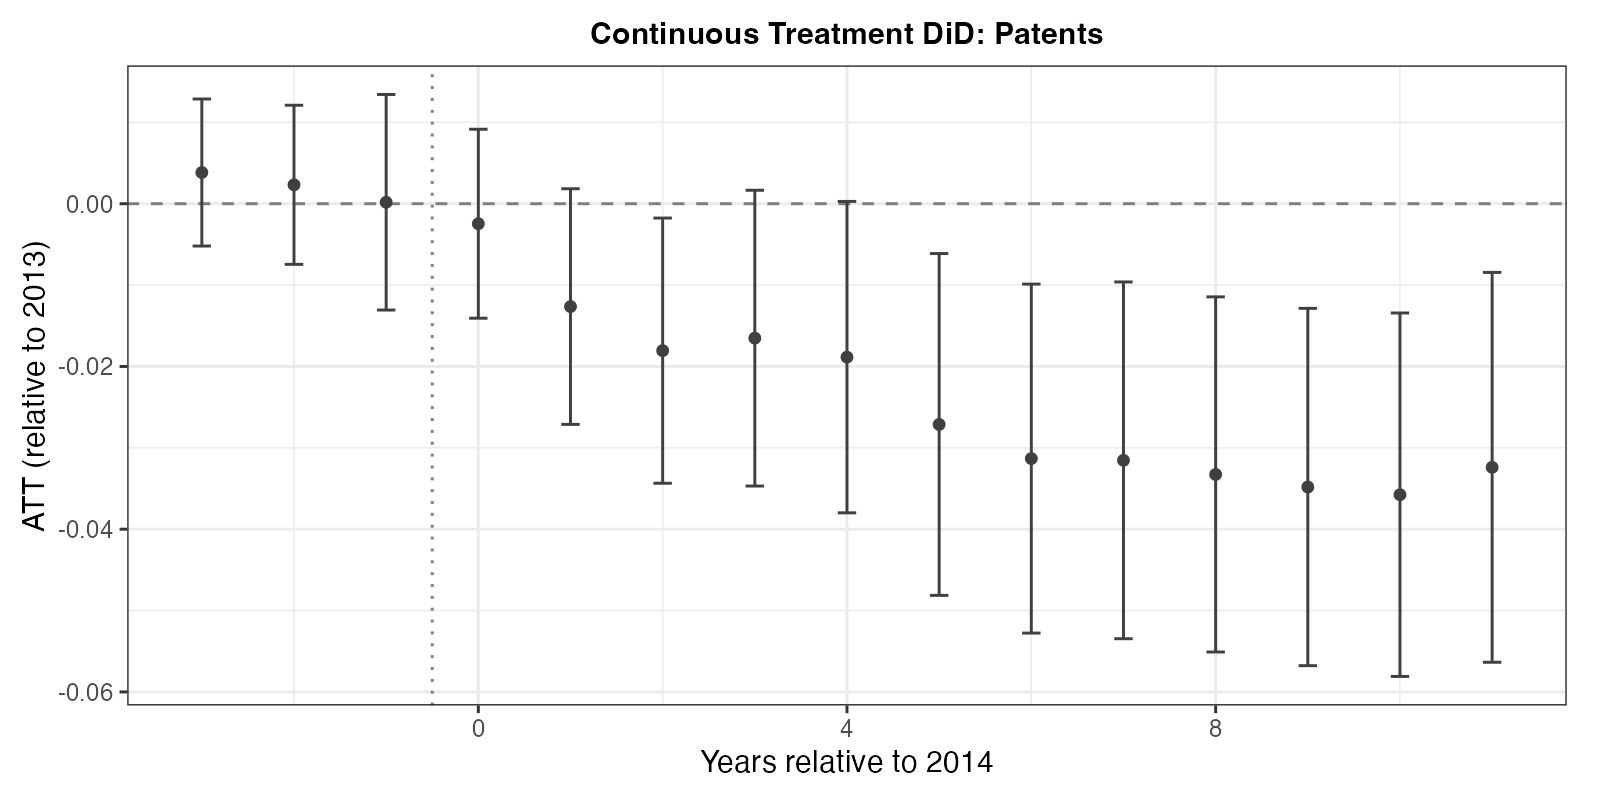
\includegraphics[width=\linewidth]{../output/robustness/contdid/contdid_patent_es.png}
  \caption{Continuous DiD event study: patents}
  \label{fig:rob_contdid_patent}
\end{figure}

\begin{figure}[!h]
  \centering
  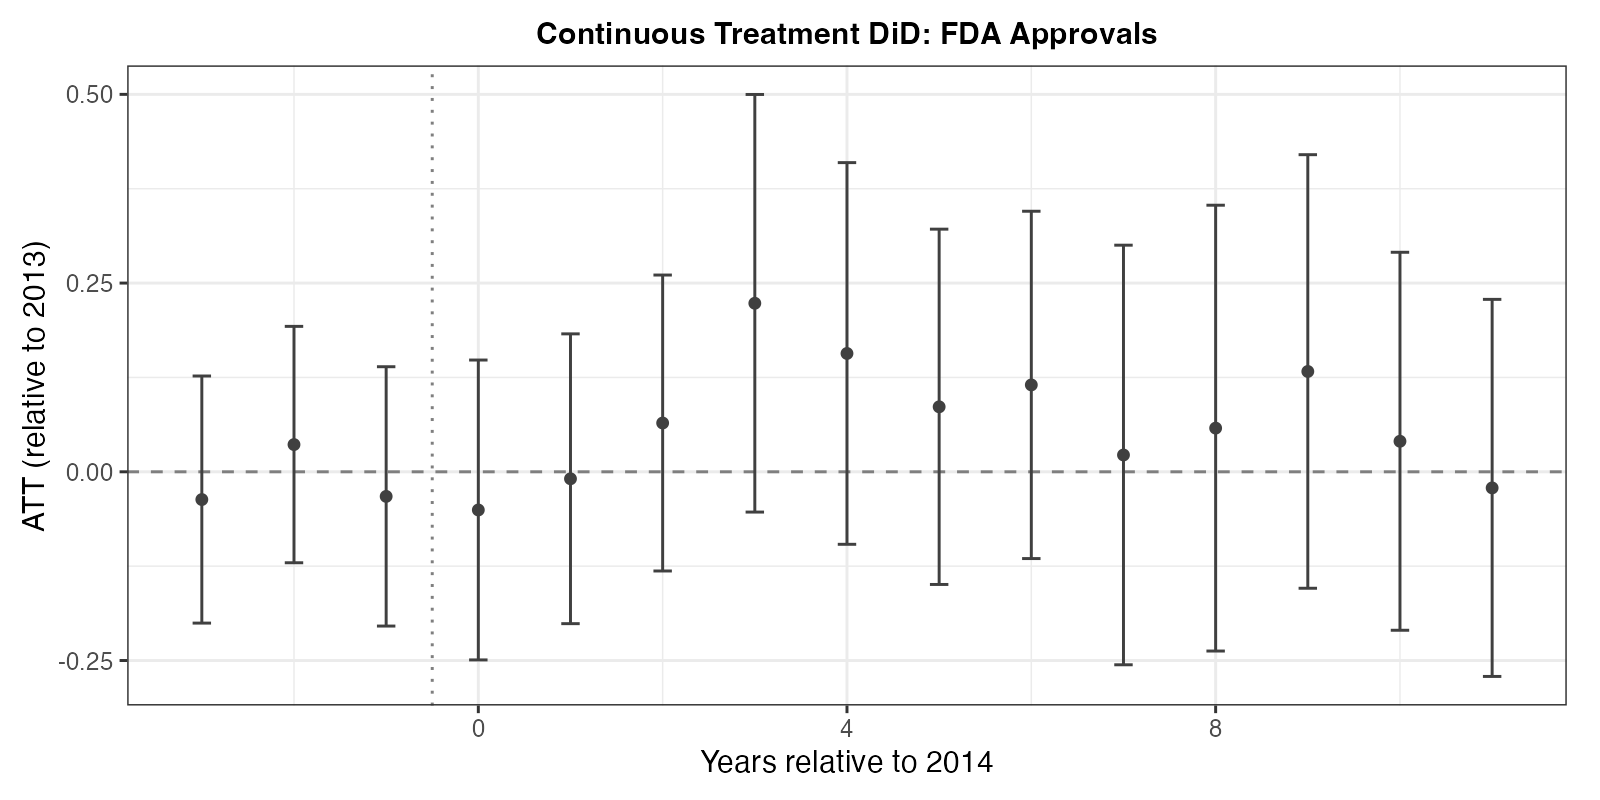
\includegraphics[width=\linewidth]{../output/robustness/contdid/contdid_fda_es.png}
  \caption{Continuous DiD event study: FDA approvals}
  \label{fig:rob_contdid_fda}
\end{figure}

\clearpage

\subsubsection{RQ2: Ex-Post FEOLS}

%TC:ignore
\footnotesize
\begin{table}
\centering
\begin{talltblr}[         %% tabularray outer open
entry=none,label=none,
note{}={* p \num{< 0.05}, ** p \num{< 0.01}, *** p \num{< 0.001}},
]                     %% tabularray outer close
{                     %% tabularray inner open
width=\linewidth,
colspec={Q[]X[]X[]X[]X[]},
column{2,3,4,5}={}{halign=c,},
column{1}={}{halign=l,},
hline{33}={1,2,3,4,5}{solid, black, 0.05em},
}                     %% tabularray inner close
\toprule
& \SetCell[c=2]{c} Patents && \SetCell[c=2]{c} FDA Approvals & \\
& Medicaid Market Share & PDL Exposure & Medicaid Market Share & PDL Exposure \\ \midrule
2010 & \num{-0.033}    & \num{1.546}     & \num{0.285}   & \num{0.046}   \\
     & (\num{0.035})   & (\num{2.018})   & (\num{0.448}) & (\num{0.807}) \\
2011 & \num{-0.010}    & \num{0.734}     & \num{0.344}   & \num{-0.257}  \\
     & (\num{0.033})   & (\num{1.642})   & (\num{0.412}) & (\num{0.711}) \\
2012 & \num{0.005}     & \num{1.079}     & \num{0.371}   & \num{1.395}   \\
     & (\num{0.027})   & (\num{1.289})   & (\num{0.447}) & (\num{0.912}) \\
2014 & \num{-0.017}    & \num{4.161}*    & \num{-0.338}  & \num{0.398}   \\
     & (\num{0.024})   & (\num{1.890})   & (\num{0.536}) & (\num{0.647}) \\
2015 & \num{-0.088}**  & \num{0.836}     & \num{-0.037}  & \num{1.158}   \\
     & (\num{0.027})   & (\num{1.480})   & (\num{0.422}) & (\num{0.881}) \\
2016 & \num{-0.123}*** & \num{-1.554}    & \num{0.456}   & \num{2.642}   \\
     & (\num{0.032})   & (\num{1.620})   & (\num{0.418}) & (\num{1.682}) \\
2017 & \num{-0.123}*** & \num{-1.342}    & \num{1.566}*  & \num{1.924}   \\
     & (\num{0.034})   & (\num{1.890})   & (\num{0.690}) & (\num{0.992}) \\
2018 & \num{-0.136}*** & \num{-2.787}    & \num{1.181}*  & \num{1.683}   \\
     & (\num{0.037})   & (\num{1.644})   & (\num{0.563}) & (\num{1.021}) \\
2019 & \num{-0.195}*** & \num{-3.807}*   & \num{0.359}   & \num{1.171}*  \\
     & (\num{0.039})   & (\num{1.912})   & (\num{0.498}) & (\num{0.591}) \\
2020 & \num{-0.227}*** & \num{-4.650}*   & \num{0.598}   & \num{1.585}   \\
     & (\num{0.041})   & (\num{1.894})   & (\num{0.537}) & (\num{0.942}) \\
2021 & \num{-0.224}*** & \num{-5.267}**  & \num{0.103}   & \num{3.110}*  \\
     & (\num{0.040})   & (\num{1.687})   & (\num{0.583}) & (\num{1.393}) \\
2022 & \num{-0.235}*** & \num{-6.029}**  & \num{0.381}   & \num{0.994}   \\
     & (\num{0.041})   & (\num{1.941})   & (\num{0.593}) & (\num{0.653}) \\
2023 & \num{-0.240}*** & \num{-6.926}*** & \num{0.798}   & \num{1.191}   \\
     & (\num{0.041})   & (\num{1.851})   & (\num{0.583}) & (\num{1.737}) \\
2024 & \num{-0.252}*** & \num{-6.485}*** & \num{0.154}   & \num{-0.447}  \\
     & (\num{0.042})   & (\num{1.788})   & (\num{0.501}) & (\num{0.589}) \\
2025 & \num{-0.212}*** & \num{-4.589}**  & \num{-0.347}  & \num{-1.113}  \\
     & (\num{0.041})   & (\num{1.549})   & (\num{0.525}) & (\num{0.908}) \\
Num. obs. & \SetCell[c=2]{c} \num{5281696} && \SetCell[c=2]{c} \num{151200} & \\
R2        & \SetCell[c=2]{c} \num{0.535}   && \SetCell[c=2]{c} \num{0.609}  & \\
\bottomrule
\end{talltblr}
\end{table}

\captionof{table}{FEOLS event-study estimates: Medicaid demand and PDL exposure (ex-post)}
\label{tab:rob_rq2_feols_expost}
\normalsize
%TC:endignore

\begin{figure}[!h]
  \centering
  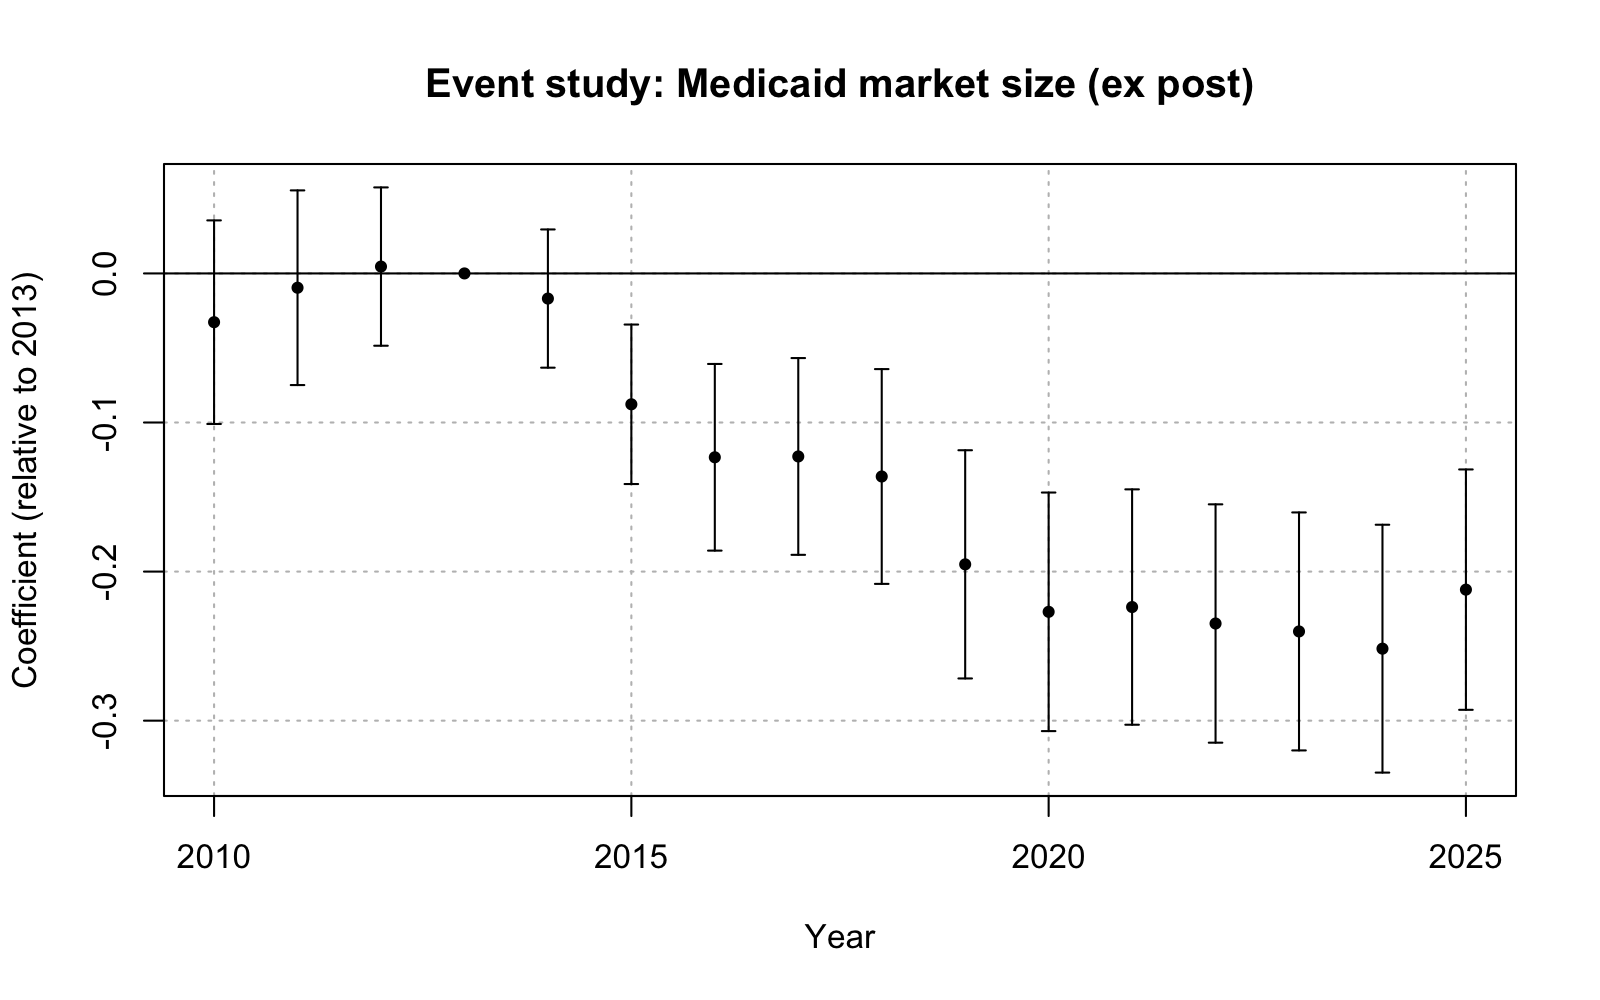
\includegraphics[width=\linewidth]{../output/RQ2/patent_feols_expost_medicaid.png}
  \caption{FEOLS event study: patents, Medicaid exposure (ex-post)}
  \label{fig:rob_rq2_patent_expost_medicaid}
\end{figure}

\begin{figure}[!h]
  \centering
  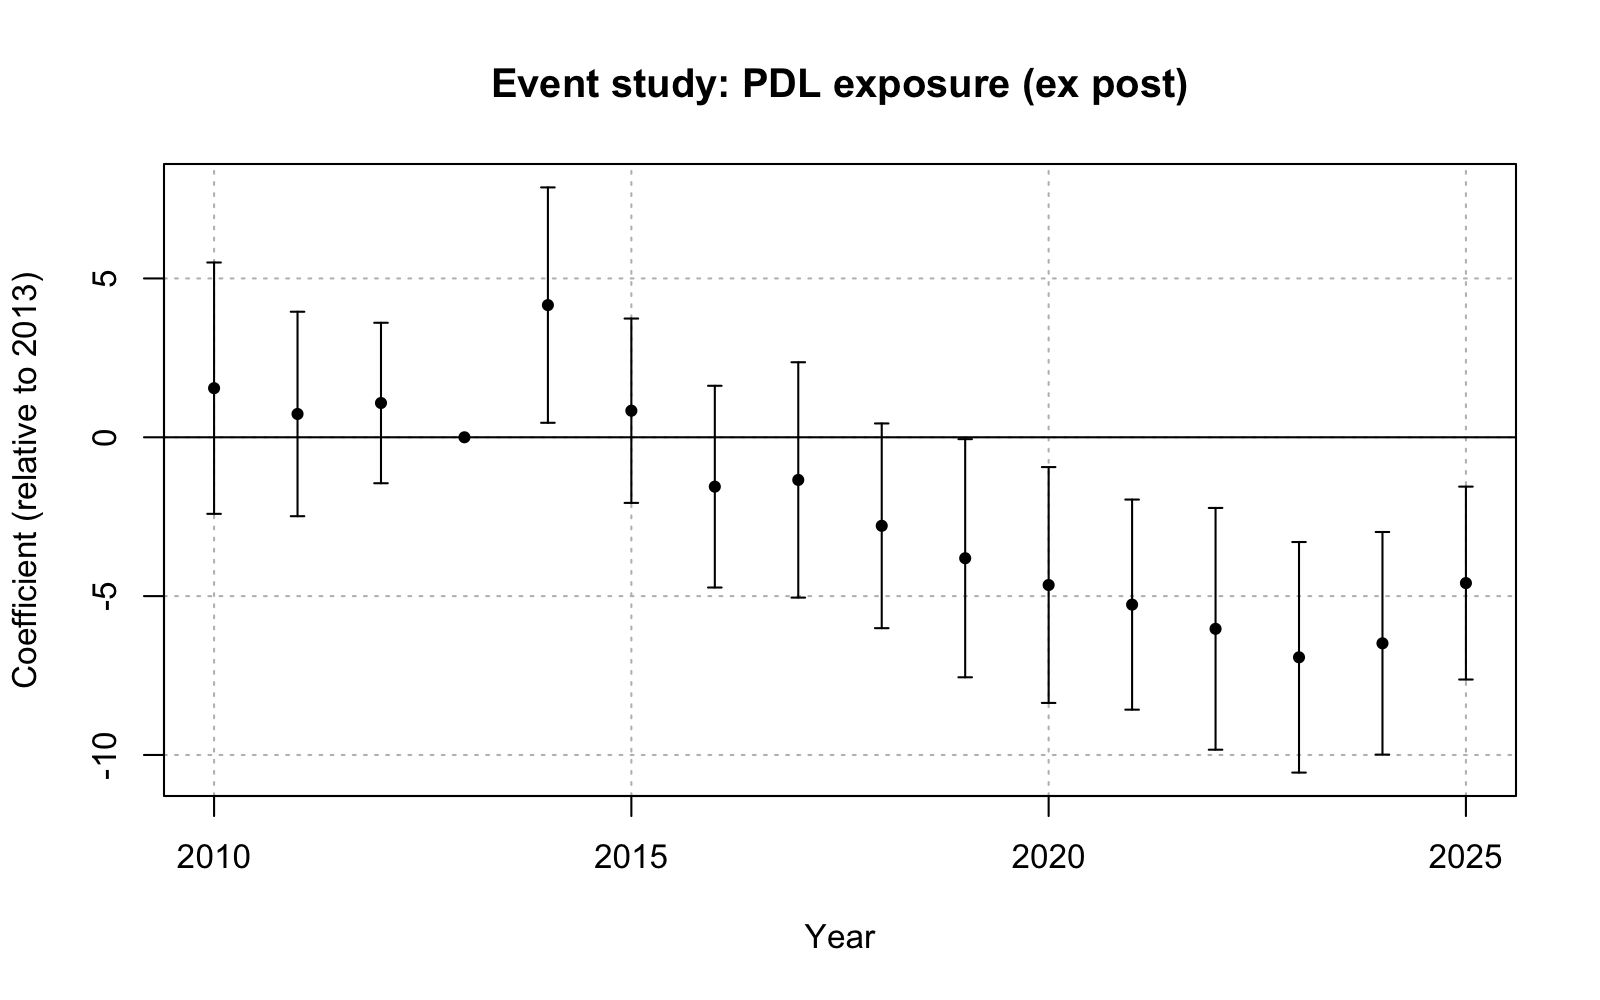
\includegraphics[width=\linewidth]{../output/RQ2/patent_feols_expost_pdl.png}
  \caption{FEOLS event study: patents, PDL exposure (ex-post)}
  \label{fig:rob_rq2_patent_expost_pdl}
\end{figure}

\clearpage

\begin{figure}[!h]
  \centering
  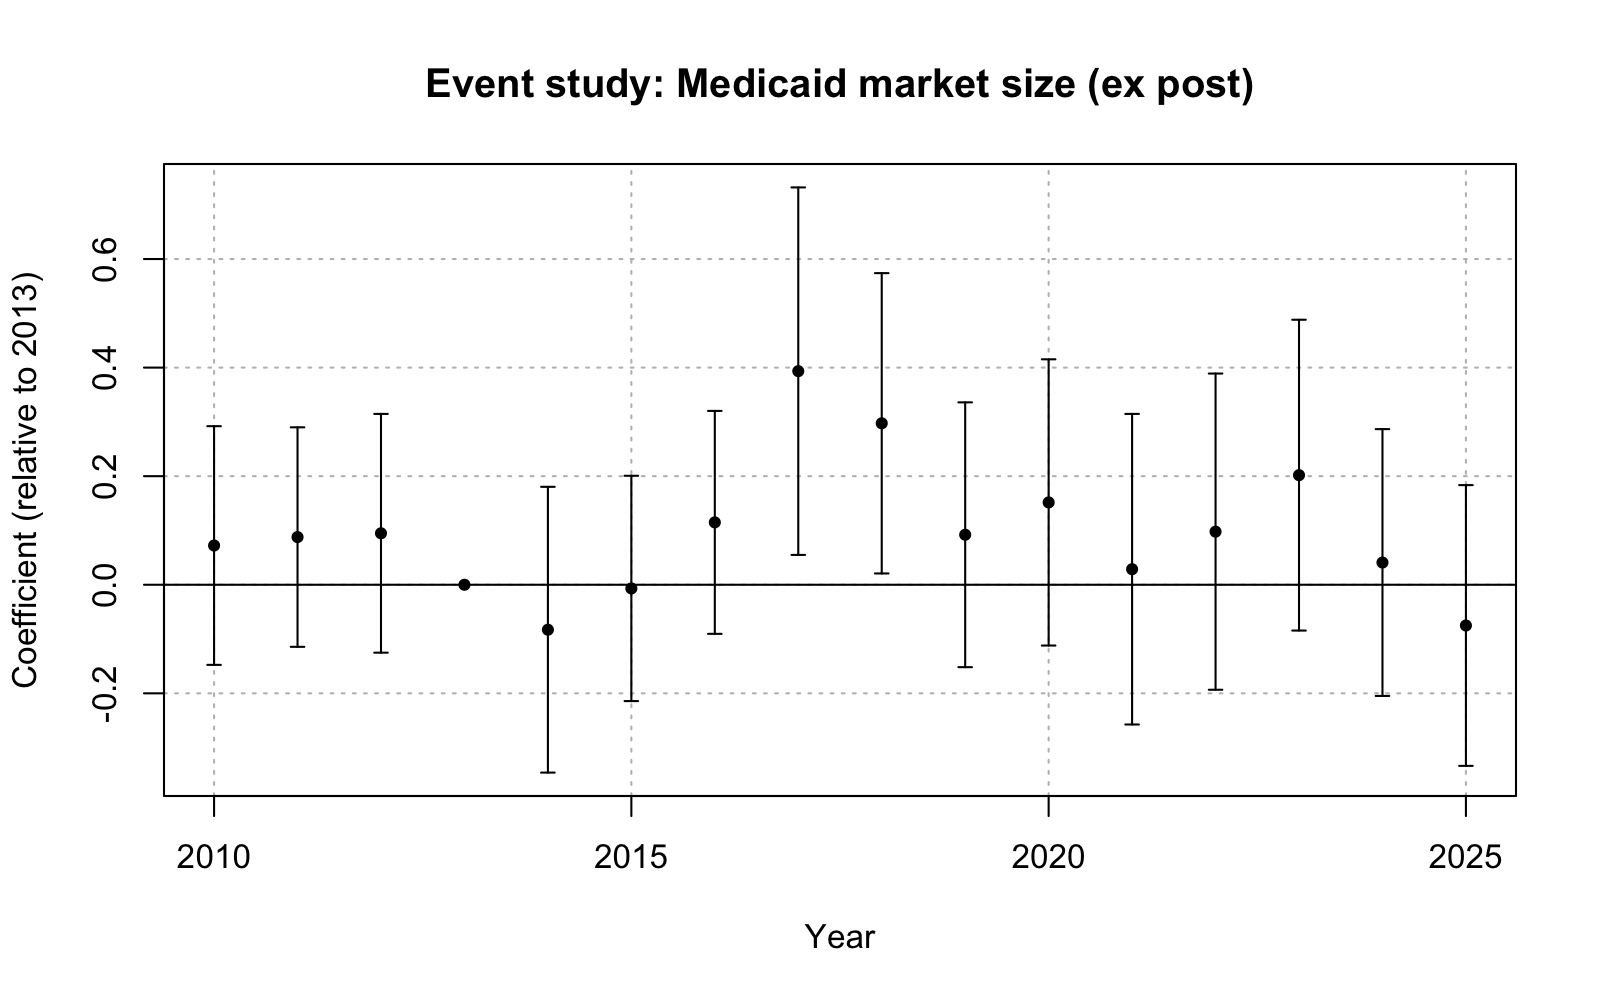
\includegraphics[width=\linewidth]{../output/RQ2/fda_feols_expost_medicaid.png}
  \caption{FEOLS event study: FDA approvals, Medicaid exposure (ex-post)}
  \label{fig:rob_rq2_fda_expost_medicaid}
\end{figure}

\begin{figure}[!h]
  \centering
  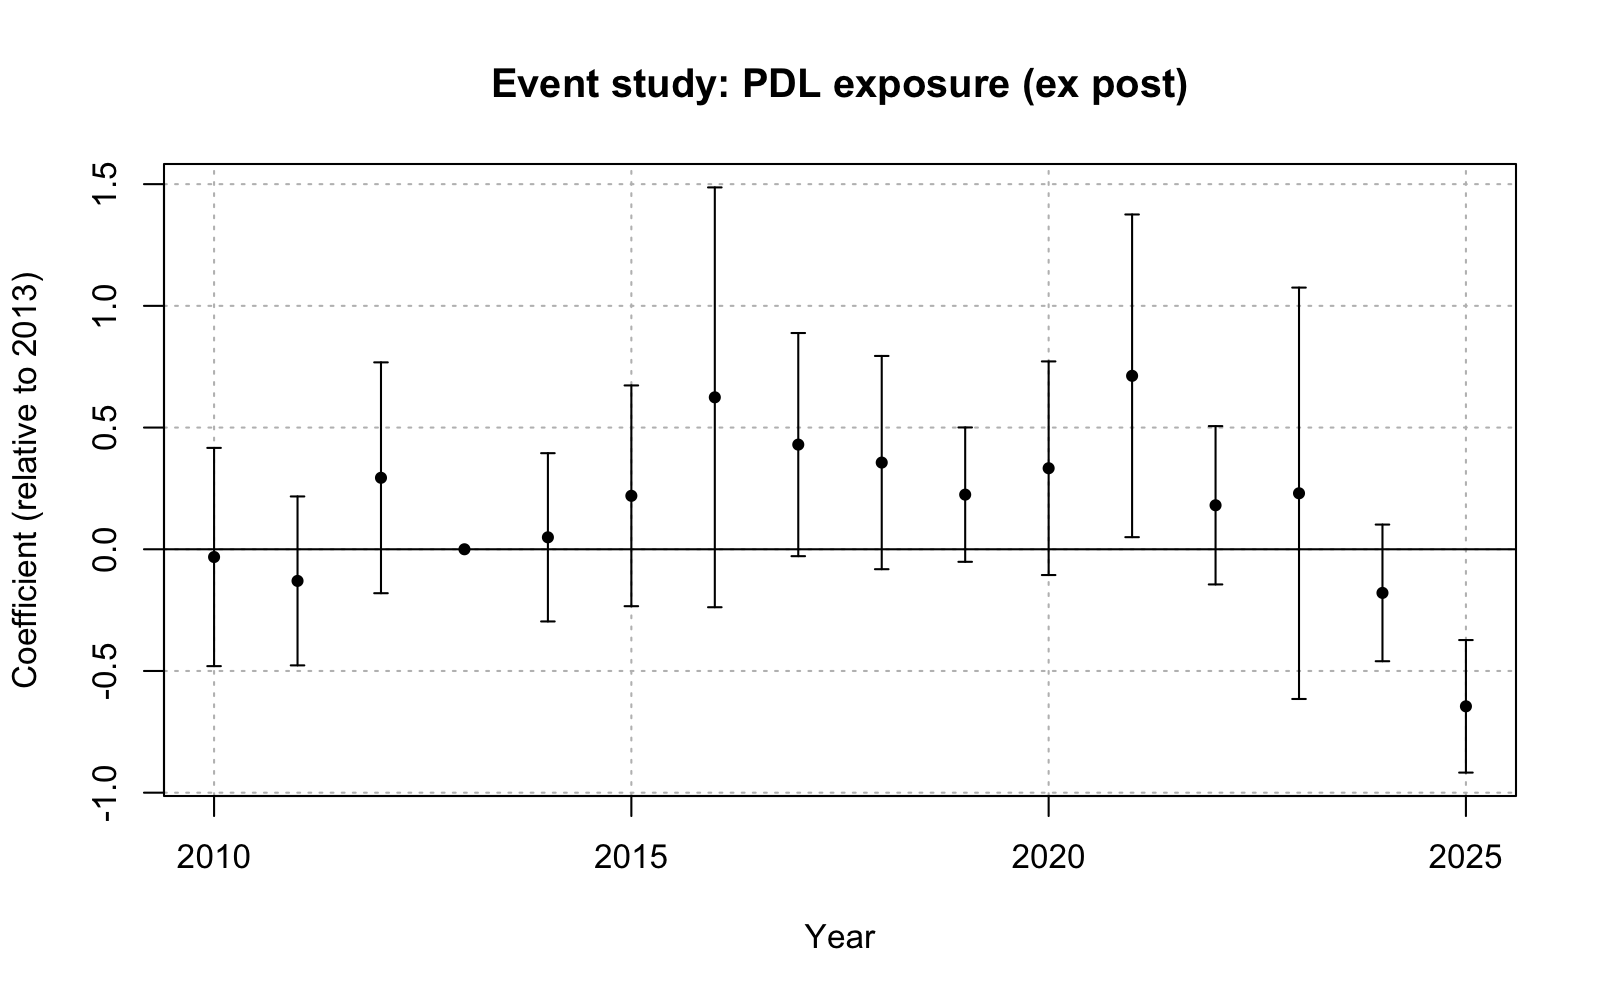
\includegraphics[width=\linewidth]{../output/RQ2/fda_feols_expost_pdl.png}
  \caption{FEOLS event study: FDA approvals, PDL exposure (ex-post)}
  \label{fig:rob_rq2_fda_expost_pdl}
\end{figure}

\clearpage

\subsubsection{RQ3: Ex-Post FEOLS}

%TC:ignore
\footnotesize
\begin{table}
\centering
\begin{talltblr}[         %% tabularray outer open
entry=none,label=none,
note{}={* p \num{< 0.05}, ** p \num{< 0.01}, *** p \num{< 0.001}},
]                     %% tabularray outer close
{                     %% tabularray inner open
colspec={Q[]Q[]Q[]},
column{2,3}={}{halign=c,},
column{1}={}{halign=l,},
hline{26}={1,2,3}{solid, black, 0.05em},
}                     %% tabularray inner close
\toprule
& Patents & FDA Approvals \\ \midrule
Medicaid Share × ATC = A & \num{-0.157}*** & \num{1.301}**  \\
& (\num{0.031})   & (\num{0.420})  \\
Medicaid Share × ATC = B & \num{0.151}***  & \num{-0.121}   \\
& (\num{0.027})   & (\num{0.784})  \\
Medicaid Share × ATC = C & \num{-0.094}*** & \num{0.373}    \\
& (\num{0.015})   & (\num{0.278})  \\
Medicaid Share × ATC = D & \num{-0.017}    & \num{0.881}**  \\
& (\num{0.062})   & (\num{0.337})  \\
Medicaid Share × ATC = G & \num{0.032}     & \num{-1.058}   \\
& (\num{0.049})   & (\num{1.121})  \\
Medicaid Share × ATC = H & \num{0.619}***  & \num{0.446}    \\
& (\num{0.096})   & (\num{0.530})  \\
Medicaid Share × ATC = J & \num{0.035}     & \num{-0.078}   \\
& (\num{0.034})   & (\num{0.089})  \\
Medicaid Share × ATC = L & \num{0.443}     & \num{-0.244}   \\
& (\num{0.578})   & (\num{2.115})  \\
Medicaid Share × ATC = M & \num{-0.212}*** & \num{0.017}    \\
& (\num{0.048})   & (\num{0.858})  \\
Medicaid Share × ATC = N & \num{-0.174}*** & \num{0.047}    \\
& (\num{0.039})   & (\num{0.101})  \\
Medicaid Share × ATC = R & \num{0.005}     & \num{0.178}    \\
& (\num{0.003})   & (\num{0.130})  \\
Medicaid Share × ATC = S & \num{0.105}***  & \num{6.473}*   \\
& (\num{0.020})   & (\num{3.004})  \\
Num. obs.                & \num{19617728}  & \num{561600}   \\
R2                       & \num{0.247}     & \num{0.235}    \\
\bottomrule
\end{talltblr}
\end{table}

\captionof{table}{Triple-difference estimates: therapeutic-class heterogeneity (FEOLS, ex-post)}
\label{tab:rob_rq3_feols_expost}
\normalsize
%TC:endignore

\clearpage

% --- From theoretical_model.tex ---

\subsection{Baseline Model Parameters} \label{app:parameters}

Table~\ref{tab:parameters} reports the baseline parameter values used to generate Figure~\ref{fig:comp_statics}. Parameters that are not varied are held at these baseline values.

%TC:ignore
\makeatletter
\renewenvironment{table}[1][H]{\@float{table}[H]}{\end@float}
\makeatother
\begin{table}[H]
\centering
\caption{Baseline parameter values used for comparative statics simulations}
\label{tab:parameters}
\begin{tblr}{
    width = \textwidth,
    colspec = {X[c,0.8] X[l,3.4] X[c,1.2]},
    row{1} = {halign=c}
}
\toprule
Parameter & Description & Baseline Value \\
\midrule
$\sigma$      & Std.\ dev.\ of the innovation shock $\varepsilon_i$                   & $1.0$           \\
$\bar{a}$     & Clinical quality threshold (P\&T approval bar)                        & $0.5$           \\
$\bar{p}$     & Regulatory price cap                                                  & $10.0$          \\
$\bar{c}$     & Expected marginal cost                                                & $2.0$           \\
$k$           & Effort cost scaling parameter                                         & $1.0$           \\
$\alpha_c$    & Rebate scale parameter                                                & $0.02$          \\
$\beta_c$     & Rebate elasticity under power form $\tau_c = \alpha_c M_c^{\beta_c}$ & $0.75$          \\
$c$           & Marginal cost distribution in the duopoly auction                     & $U[0.5,\, 3.5]$ \\
$M_0$         & Reference market size                                                 & $100$           \\
$\delta$      & Period 2 cost reduction factor                                        & $0.7$           \\
\bottomrule
\end{tblr}
\end{table}
\renewenvironment{table}[1][]{}{}
%TC:endignore

\end{document}
